\documentclass[]{report}
\usepackage[utf8]{inputenc}
\usepackage{geometry}
\geometry{a4paper,left=2cm,right=3cm, top=2cm, bottom=2cm} 


\usepackage{amsmath}
\usepackage{siunitx}
\usepackage{graphicx}
\usepackage{caption}
\usepackage{subcaption}

\usepackage{pgfplots}
% and optionally (as of Pgfplots 1.3):
\pgfplotsset{compat=newest}
\pgfplotsset{plot coordinates/math parser=false}
\newlength\figureheight
\newlength\figurewidth 
\setlength\figureheight{5cm}
\setlength\figurewidth{\textwidth}


\renewcommand\floatpagefraction{.99}


% Title Page
\title{Gruppennummer 16}
\author{Andreas Cremer\\Hanna Huber (0925230) \\Lena Trautmann (1526567)}



\begin{document}
	\maketitle
	
	%\begin{abstract}
	%\end{abstract}
	
	\begin{enumerate}
		\item Kovarianzmatrix
		\begin{enumerate}
			\item
			ourCov.m erwartet eine $d \times n$ Matrix und gibt die dazugehörige Kovarianzmatrix zurück.
			\item
			\setlength\figureheight{5cm}
			\setlength\figurewidth{.4\textwidth}
			\begin{figure}
				\begin{subfigure}{0.45\textwidth}
					\centering
					% This file was created by matlab2tikz.
% Minimal pgfplots version: 1.3
%
%The latest updates can be retrieved from
%  http://www.mathworks.com/matlabcentral/fileexchange/22022-matlab2tikz
%where you can also make suggestions and rate matlab2tikz.
%
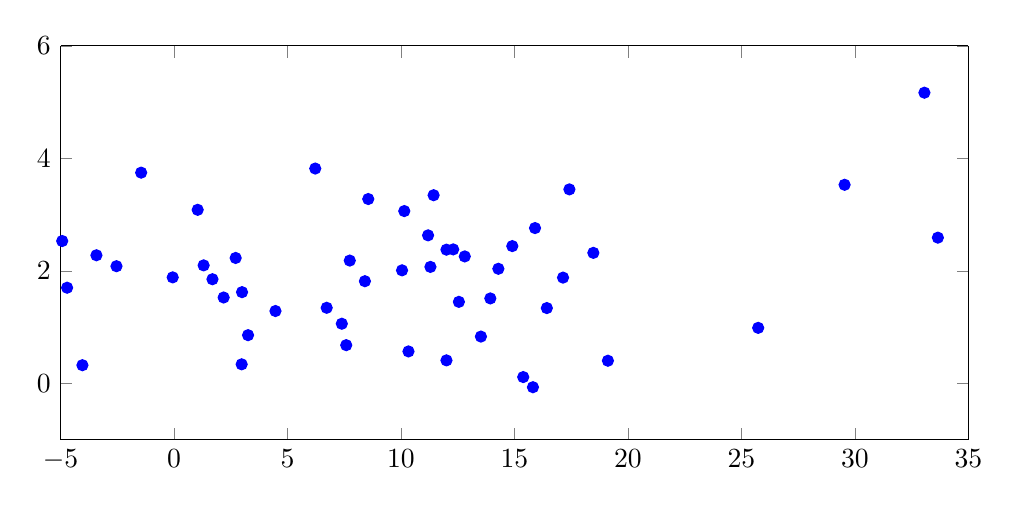
\begin{tikzpicture}

\begin{axis}[%
width=0.95092\figurewidth,
height=\figureheight,
at={(0\figurewidth,0\figureheight)},
scale only axis,
separate axis lines,
every outer x axis line/.append style={black},
every x tick label/.append style={font=\color{black}},
xmin=-5,
xmax=35,
every outer y axis line/.append style={black},
every y tick label/.append style={font=\color{black}},
ymin=-1,
ymax=6
]
\addplot [color=blue,only marks,mark=*,mark options={solid},forget plot]
  table[row sep=crcr]{%
7.74416883153805	2.18160318122483\\
2.71635996888923	2.22787984441007\\
-1.44682787033701	3.74471993350627\\
6.22312688197506	3.81787413004095\\
10.1462590349818	3.06163290459646\\
1.04328725190157	3.08398538559699\\
13.5223937459084	0.830327990864534\\
8.55871992530961	3.27577346884409\\
7.3934360555112	1.05842760202118\\
19.1173328995951	0.400549584371423\\
33.0618242015673	5.16625311280659\\
18.4764343762861	2.31866731206772\\
16.4269086947992	1.33706332414892\\
10.0472004464365	2.00792589456022\\
11.2978651215934	2.06900941910027\\
15.8142927241028	-0.0700280325852325\\
4.47019717021839	1.2844499359472\\
-4.92558795155322	2.52931945336738\\
14.291118571226	2.03554031115133\\
2.98133750013824	0.337105143552666\\
13.9371699200445	1.50850767011705\\
1.69457735088906	1.84993312130601\\
-2.53417173336777	2.08133234660466\\
-4.0343011722622	0.321223028710933\\
12.8110146188365	2.25533608712195\\
29.5453920046404	3.52905134358035\\
12.0043804637693	0.407273397737469\\
14.9050351854076	2.43879028982054\\
11.4380903424203	3.34365141705886\\
12.3009588569895	2.38034770828384\\
33.6547508923074	2.5890642548347\\
2.18731785579572	1.52496179181873\\
8.41110726686743	1.81481096531118\\
3.26290647600352	0.85528457649676\\
17.140481938103	1.87849393853717\\
12.5518923678767	1.44738202416548\\
6.72737712669883	1.34196722437491\\
17.4210709381367	3.44725099802365\\
-0.0570393532845763	1.88294263537276\\
11.1942067727222	2.62993479002457\\
12.0044175628734	2.37530719610252\\
25.7385123860363	0.985112664307279\\
15.386275774621	0.110141784013792\\
10.3306070700226	0.566243507942441\\
-3.4174608032206	2.27594102271539\\
-4.70908406934728	1.69879197463575\\
15.9063095137358	2.75950290888421\\
2.99816380826258	1.62005251511655\\
7.58809288784172	0.677697069519529\\
1.30583031594183	2.0963315771043\\
};
\end{axis}
\end{tikzpicture}%
					\caption{$C_{1}$}
					\label{fig:cov1}
				\end{subfigure}
				\qquad
				\begin{subfigure}{0.45\textwidth}
					\centering
					% This file was created by matlab2tikz.
% Minimal pgfplots version: 1.3
%
%The latest updates can be retrieved from
%  http://www.mathworks.com/matlabcentral/fileexchange/22022-matlab2tikz
%where you can also make suggestions and rate matlab2tikz.
%
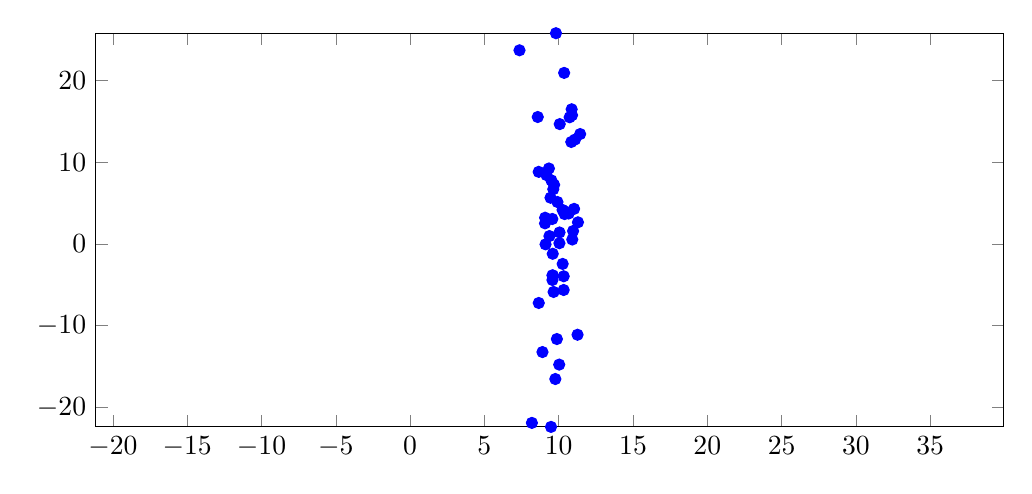
\begin{tikzpicture}

\begin{axis}[%
width=0.95092\figurewidth,
height=\figureheight,
at={(0\figurewidth,0\figureheight)},
scale only axis,
separate axis lines,
every outer x axis line/.append style={black},
every x tick label/.append style={font=\color{black}},
xmin=-21.1445645281725,
xmax=39.9493114253335,
every outer y axis line/.append style={black},
every y tick label/.append style={font=\color{black}},
ymin=-22.3920614159571,
ymax=25.7932697796306
]
\addplot [color=blue,only marks,mark=*,mark options={solid},forget plot]
  table[row sep=crcr]{%
11.1010479159111	12.7800634320016\\
10.2654188321564	-2.44330361217242\\
9.81404464074737	25.7932697796306\\
9.57906683577328	-4.40975418360709\\
11.2681221143578	-11.1128158936808\\
10.9143071564477	0.543119389031014\\
9.57034854448887	3.05785035897782\\
8.65360615685203	8.82352297722657\\
9.08644963621784	3.21039798364379\\
10.3333266941572	-5.63621147141663\\
8.90741123358919	-13.2302307169266\\
9.61304889167535	-3.86692932017392\\
9.87756482231943	-11.6374394474195\\
9.34022247738409	9.2359479144432\\
9.37552256089639	0.963724228664804\\
9.77368751744229	-16.5300581823224\\
9.44915904634767	5.65594674805797\\
8.65773491758514	-7.22408106838758\\
10.7365892484148	15.5037753365345\\
9.08045112598076	2.52197866672478\\
11.0350392949792	4.29233268833437\\
9.65659262959267	-5.87379336657145\\
9.69211714235693	7.23016403037701\\
11.2955708256022	2.64903038833475\\
10.2610885572818	4.16167132064005\\
9.59772759848202	-1.20273392593171\\
9.17304435319498	8.43380002762061\\
9.48278292283401	-22.3920614159571\\
10.3999093669464	3.65680347857051\\
10.8471342331179	12.4820655515325\\
10.0480109567023	0.0933335437170495\\
9.5070769245243	7.7813357919509\\
10.3354370751796	-3.95495257205553\\
10.6712144486512	3.72748217456145\\
9.57833764771	-3.83976906010968\\
11.4431265027622	13.4502586032493\\
9.63571900872759	6.69942835626373\\
10.8982881506395	15.7592677222661\\
10.9683438281307	1.58240117725563\\
10.0566274263604	1.40690766570213\\
9.91533353408232	5.13304071328229\\
10.8720104110242	16.4839070468213\\
8.19634467273942	-21.9014784705216\\
10.0337400768363	-14.7655395603042\\
10.0691386095133	14.6675318025445\\
10.365586778607	20.9353452902617\\
9.11514030504879	-0.0477382308846677\\
8.58982463397439	15.5381342933836\\
7.36162039439881	23.7019327014232\\
10.545101683344	3.89695984371778\\
};
\end{axis}
\end{tikzpicture}%
					\caption{$C_{2}$}
					\label{fig:cov2}
				\end{subfigure}	
				\\
				\begin{subfigure}{0.45\textwidth}
					\centering
					% This file was created by matlab2tikz.
% Minimal pgfplots version: 1.3
%
%The latest updates can be retrieved from
%  http://www.mathworks.com/matlabcentral/fileexchange/22022-matlab2tikz
%where you can also make suggestions and rate matlab2tikz.
%
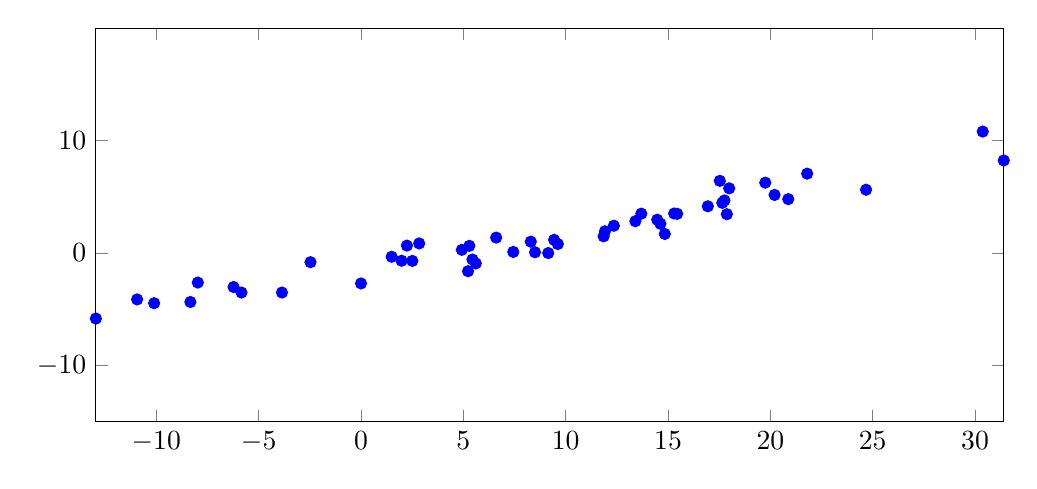
\begin{tikzpicture}

\begin{axis}[%
width=0.95092\figurewidth,
height=\figureheight,
at={(0\figurewidth,0\figureheight)},
scale only axis,
separate axis lines,
every outer x axis line/.append style={black},
every x tick label/.append style={font=\color{black}},
xmin=-12.953226877787,
xmax=31.401608574977,
every outer y axis line/.append style={black},
every y tick label/.append style={font=\color{black}},
ymin=-15.0059436067627,
ymax=19.9771443551754
]
\addplot [color=blue,only marks,mark=*,mark options={solid},forget plot]
  table[row sep=crcr]{%
5.44472978269709	-0.577289933813434\\
5.22805993100385	-1.61349419707251\\
7.43870466825692	0.100336381683103\\
17.9867387828379	5.75031853523774\\
8.29352813628289	1.01157140895627\\
30.3730913354772	10.7926493491835\\
6.60318793578978	1.37177345507569\\
2.84143991718599	0.856429263381885\\
15.4451966610762	3.48756508581657\\
12.3531091903292	2.42635440824064\\
14.6252626849383	2.60421079873865\\
-10.9387635929438	-4.12081253325755\\
8.49997477137822	0.0670570937670636\\
-8.33525474571426	-4.35064291141613\\
11.8533876174123	1.48679170628117\\
17.6498906665636	4.46330552161421\\
21.7957902617132	7.0546388980878\\
17.5296775004699	6.41643212919879\\
14.8407754035302	1.6965304618198\\
17.7543759736931	4.67306011027556\\
9.43338702977036	1.17591462388934\\
9.61498587566128	0.803017651447581\\
20.2044747193525	5.16472265010514\\
20.8728389278498	4.78998728434885\\
5.29169777657604	0.638628144502255\\
-7.97279740485603	-2.62333345417865\\
-12.953226877787	-5.82144860077072\\
-6.22578573194761	-3.02044631926593\\
-0.000719054247699802	-2.70057294974776\\
14.4711755856635	2.95810012862123\\
2.24159088802308	0.66132907044002\\
9.14665607150171	-0.00170154930304056\\
13.6939096941233	3.49902389303887\\
-3.86210853860879	-3.51063256772806\\
1.49750180459497	-0.33175520459092\\
2.50618354370613	-0.698436589563464\\
1.98210580859646	-0.683896919629093\\
5.60750581178614	-0.921637027767139\\
17.8717947302458	3.45046983270511\\
4.92528953683873	0.284565540228405\\
16.9431050270731	4.15461037217091\\
13.4032700587016	2.82966763240154\\
11.9185584382323	1.93433790779544\\
19.7503240575992	6.25365189610861\\
31.401608574977	8.22601915643582\\
24.6733281566119	5.62610157558818\\
-5.84033827180256	-3.51074860674999\\
15.2991185966086	3.51413691363539\\
-2.46844330524427	-0.811528812240311\\
-10.1079630699076	-4.45695644857533\\
};
\end{axis}
\end{tikzpicture}%
					\caption{$C_{3}$}
					\label{fig:cov3}
				\end{subfigure}
				\qquad
				\begin{subfigure}{0.45\textwidth}
					\centering
					% This file was created by matlab2tikz.
% Minimal pgfplots version: 1.3
%
%The latest updates can be retrieved from
%  http://www.mathworks.com/matlabcentral/fileexchange/22022-matlab2tikz
%where you can also make suggestions and rate matlab2tikz.
%
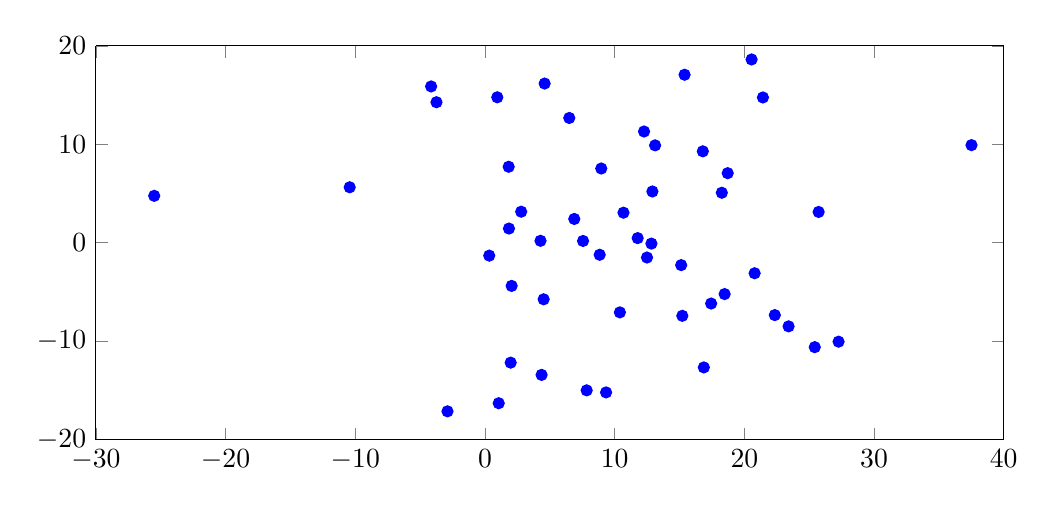
\begin{tikzpicture}

\begin{axis}[%
width=0.95092\figurewidth,
height=\figureheight,
at={(0\figurewidth,0\figureheight)},
scale only axis,
separate axis lines,
every outer x axis line/.append style={black},
every x tick label/.append style={font=\color{black}},
xmin=-30,
xmax=40,
every outer y axis line/.append style={black},
every y tick label/.append style={font=\color{black}},
ymin=-20,
ymax=20
]
\addplot [color=blue,only marks,mark=*,mark options={solid},forget plot]
  table[row sep=crcr]{%
18.7156557243306	7.06059506234169\\
12.265244553888	11.2921146138128\\
4.36673989443474	-13.4349783131208\\
1.82777791632296	7.71055922213634\\
11.7734404598447	0.460780474919601\\
8.96672983503264	7.53328570799877\\
0.950094104596426	14.7678425960038\\
2.0565735372081	-4.3941237685512\\
15.3912820294882	17.0593483426331\\
15.2166391689867	-7.43393573397202\\
6.88599604829554	2.40831693453769\\
18.2612770354213	5.06955631164682\\
6.5005934102686	12.6682307672474\\
8.84497310049439	-1.23146333398642\\
22.3482171829568	-7.35874145579186\\
4.60079013541161	16.1661411698876\\
-10.4295541608974	5.62642928190036\\
-2.88880154150336	-17.1367787710994\\
12.9084875627763	5.19922422174947\\
7.84207756680738	-15.0058679799209\\
37.5134027656672	9.9091598831421\\
-4.15076615934147	15.8716658481553\\
7.56130990949062	0.17222125136134\\
10.4025070078518	-7.08393356847147\\
-3.73829429801884	14.2692984951034\\
20.7918731483707	-3.10703299406317\\
17.4393115949833	-6.18471951493772\\
25.4286065009815	-10.6177054406154\\
16.875221467436	-12.6764802945527\\
-25.501683039025	4.75779186692215\\
0.329468473982711	-1.31746313840677\\
13.1179042820021	9.88484408845746\\
1.8493105713285	1.43306034580109\\
12.8337045148214	-0.0968647255023156\\
9.33762135282234	-15.2146551394431\\
4.52503215581019	-5.75463907445961\\
10.6805624790237	3.04429626048291\\
15.1297373621053	-2.28145137621409\\
21.4309605165656	14.7504684048415\\
1.06054882586093	-16.3143051877386\\
4.28227561922965	0.188020609456912\\
2.79356977649472	3.1457557491049\\
18.4789601029615	-5.2235759714857\\
25.7262685395206	3.12002827504684\\
20.5572101931724	18.6126749449529\\
23.4101376686318	-8.50388785955973\\
12.4927537344373	-1.50881516799212\\
1.98294160728703	-12.1908054304414\\
16.7974785394543	9.27937514727138\\
27.2637983804176	-10.0605463167353\\
};
\end{axis}
\end{tikzpicture}%
					\caption{$C_{4}$}
					\label{fig:cov4}
				\end{subfigure}	
				\caption{Die Daten aus data1 (a), data2 (b), data3 (c) and data4 (d)}
				\label{fig:cov}
			\end{figure}
			
			Hier werden die Kovarianzmatrizen für daten.mat berechnet. In $C_{11}$ steht die Varianz in der ersten Dimension. In $C_{22}$ steht die Varianz in der zweiten Dimension. In $C_{12}$ und $C_{21}$ steht die Kovarianz.\\
			Abbildung~\ref{fig:cov} zeigt die verschiedenen 2D-Datensätze. data1 hat eine hohe Varianz in der ersten und eine geringe Varianz in der zweiten Dimension. Die Kovarianz ist gering, die Datenpunkte bilden ein schmales Band parallel zur x-Achse.\\
			data2 hat eine geringe Varianz in der ersten und eine hohe Varianz in der zweiten Dimension und ebenfalls eine geringe Kovarianz. Die Datenpunkte bilden ein schmales Band parallel zur y-Achse.\\
			data3 hat eine sehr hohe und eine deutlich niedrigere Varianz sowie eine hohe Kovarianz. Dies führt zu einem leicht ansteigenden Band.\\
			data4 hat hohe nahe beieinander liegende Varianzen und eine Kovarianz nahe beim Nullpunkt. Dies führt zu einer Punktwolke ohne erkennbare Ordnung.
		\end{enumerate}
		\item PCA\\
		
		pca.m berechnet die PCA indem mithilfe von der Matlabfunktion eig die Eigenwerte und -vektoren abgefragt werden. Diese Funktion ordnet beides nach aufsteigenden Eigenwerten, daher wird danach noch die Reihenfolge umgekehrt.
		\begin{enumerate}
			
			\item
			\setlength\figureheight{5cm}
			\setlength\figurewidth{.4\textwidth}
			\begin{figure}
				\begin{subfigure}{0.45\textwidth}
					\centering
					% This file was created by matlab2tikz.
% Minimal pgfplots version: 1.3
%
%The latest updates can be retrieved from
%  http://www.mathworks.com/matlabcentral/fileexchange/22022-matlab2tikz
%where you can also make suggestions and rate matlab2tikz.
%
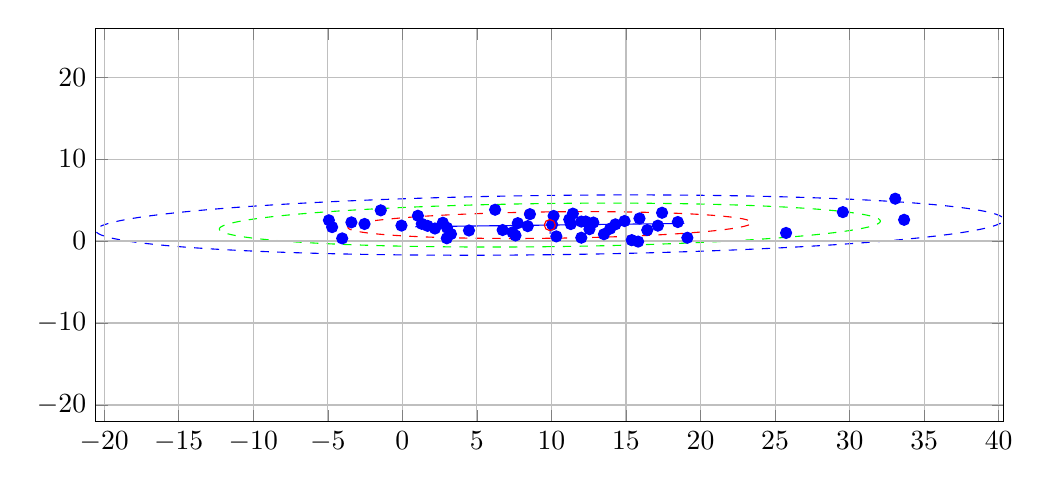
\begin{tikzpicture}

\begin{axis}[%
width=0.95092\figurewidth,
height=\figureheight,
at={(0\figurewidth,0\figureheight)},
scale only axis,
separate axis lines,
every outer x axis line/.append style={black},
every x tick label/.append style={font=\color{black}},
xmin=-20.5551589262013,
xmax=40.3413081320193,
xmajorgrids,
every outer y axis line/.append style={black},
every y tick label/.append style={font=\color{black}},
ymin=-22.067001610149,
ymax=25.9626312793185,
ymajorgrids,
every outer z axis line/.append style={black},
every z tick label/.append style={font=\color{black}},
zmin=-0.700740822236688,
zmax=1.70074082223669,
zmajorgrids,
view={0}{90},
legend style={legend cell align=left,align=left,draw=black}
]
\addplot [color=blue,only marks,mark=*,mark options={solid}]
  table[row sep=crcr]{%
7.74416883153805	2.18160318122483\\
2.71635996888923	2.22787984441007\\
-1.44682787033701	3.74471993350627\\
6.22312688197506	3.81787413004095\\
10.1462590349818	3.06163290459646\\
1.04328725190157	3.08398538559699\\
13.5223937459084	0.830327990864534\\
8.55871992530961	3.27577346884409\\
7.3934360555112	1.05842760202118\\
19.1173328995951	0.400549584371423\\
33.0618242015673	5.16625311280659\\
18.4764343762861	2.31866731206772\\
16.4269086947992	1.33706332414892\\
10.0472004464365	2.00792589456022\\
11.2978651215934	2.06900941910027\\
15.8142927241028	-0.0700280325852325\\
4.47019717021839	1.2844499359472\\
-4.92558795155322	2.52931945336738\\
14.291118571226	2.03554031115133\\
2.98133750013824	0.337105143552666\\
13.9371699200445	1.50850767011705\\
1.69457735088906	1.84993312130601\\
-2.53417173336777	2.08133234660466\\
-4.0343011722622	0.321223028710933\\
12.8110146188365	2.25533608712195\\
29.5453920046404	3.52905134358035\\
12.0043804637693	0.407273397737469\\
14.9050351854076	2.43879028982054\\
11.4380903424203	3.34365141705886\\
12.3009588569895	2.38034770828384\\
33.6547508923074	2.5890642548347\\
2.18731785579572	1.52496179181873\\
8.41110726686743	1.81481096531118\\
3.26290647600352	0.85528457649676\\
17.140481938103	1.87849393853717\\
12.5518923678767	1.44738202416548\\
6.72737712669883	1.34196722437491\\
17.4210709381367	3.44725099802365\\
-0.0570393532845763	1.88294263537276\\
11.1942067727222	2.62993479002457\\
12.0044175628734	2.37530719610252\\
25.7385123860363	0.985112664307279\\
15.386275774621	0.110141784013792\\
10.3306070700226	0.566243507942441\\
-3.4174608032206	2.27594102271539\\
-4.70908406934728	1.69879197463575\\
15.9063095137358	2.75950290888421\\
2.99816380826258	1.62005251511655\\
7.58809288784172	0.677697069519529\\
1.30583031594183	2.0963315771043\\
};
%\addlegendentry{Daten};

\addplot [color=red,only marks,mark=o,mark options={solid}]
  table[row sep=crcr]{%
9.89307460290898	1.94781483458474\\
};
%\addlegendentry{Mittelwert};

\addplot [color=blue,solid]
  table[row sep=crcr]{%
18.9166371472202	2.14817452823074\\
0.869512058597788	1.74745514093875\\
};
%\addlegendentry{Eigenvektoren};

\addplot [color=blue,solid]
  table[row sep=crcr]{%
9.8692784641791	3.01951714274238\\
9.91687074163886	0.876112526427109\\
};
%\addlegendentry{};

\addplot3 [color=red,dashed]
 table[row sep=crcr] {%
9.92878271214284	0.339635309315125	1\\
9.50344409155438	0.330984997248743	1\\
9.07848998923997	0.323930301029581	1\\
8.65433978359326	0.318478182791081	1\\
8.23141205965894	0.314634023115704	1\\
7.81012419603986	0.312401615724938	1\\
7.39089195299472	0.311783163735355	1\\
6.97412906213286	0.312779277484404	1\\
6.56024681811119	0.315388973928077	1\\
6.14965367273593	0.319609677611054	1\\
5.74275483187007	0.325437223208374	1\\
5.33995185554405	0.332865859636099	1\\
4.94164226166451	0.341888255726946	1\\
4.5482191337121	0.352495507465261	1\\
4.16007073281557	0.364677146774205	1\\
3.77758011458488	0.37842115184649	1\\
3.40112475108156	0.393713959008441	1\\
3.0310761582994	0.410540476105714	1\\
2.66779952952295	0.428884097397423	1\\
2.31165337492591	0.448726719944006	1\\
1.9629891677648	0.470048761472637	1\\
1.62215099751737	0.49282917970257	1\\
1.28947523030775	0.517045493111325	1\\
0.965290176953742	0.542673803121239	1\\
0.649915768963679	0.569688817684473	1\\
0.343663242802631	0.598063876243219	1\\
0.0468348327396022	0.627770976040439	1\\
-0.240276527421203	0.658780799755216	1\\
-0.517387493430679	0.691062744435405	1\\
-0.78422459022139	0.724584951699053	1\\
-1.04052448179444	0.759314339174775	1\\
-1.28603423110029	0.795216633150063	1\\
-1.52051154965715	0.8322564023953	1\\
-1.74372503666038	0.870397093130107	1\\
-1.9554544073472	0.909601065097508	1\\
-2.15549071039113	0.949829628710326	1\\
-2.34363653411177	0.991043083233129	1\\
-2.5197062012962	1.03320075596206	1\\
-2.68352595244007	1.0762610423639	1\\
-2.8349341172272	1.12018144713469	1\\
-2.97378127407866	1.16491862613751	1\\
-3.09993039761388	1.21042842917786	1\\
-3.21325699387807	1.25666594357461	1\\
-3.31364922320284	1.30358553848337	1\\
-3.40100801057832	1.35114090992863	1\\
-3.47524714342834	1.39928512650022	1\\
-3.53629335669176	1.44797067566889	1\\
-3.5840864051263	1.49714951067549	1\\
-3.61857912276328	1.54677309794731	1\\
-3.63973746945474	1.59679246499483	1\\
-3.64754056446698	1.6471582487417	1\\
-3.6419807070873	1.69782074424008	1\\
-3.62306338422368	1.74872995372348	1\\
-3.59080726498988	1.79983563594848	1\\
-3.54524418228125	1.85108735577679	1\\
-3.48641910135953	1.90243453394863	1\\
-3.41439007547754	1.95382649699837	1\\
-3.32922818858767	2.00521252726311	1\\
-3.23101748519055	2.05654191293487	1\\
-3.11985488739332	2.10776399810709	1\\
-2.99585009925918	2.15882823276581	1\\
-2.85912549854273	2.20968422267648	1\\
-2.70981601591792	2.26028177911697	1\\
-2.54806900181776	2.31057096840781	1\\
-2.37404408101721	2.36050216119064	1\\
-2.1879129951028	2.41002608140645	1\\
-1.98985943298447	2.45909385492509	1\\
-1.78007884961672	2.50765705777812	1\\
-1.55877827310822	2.55566776394743	1\\
-1.32617610041005	2.60307859266243	1\\
-1.08250188178425	2.64984275515916	1\\
-0.827996094265469	2.69591410085514	1\\
-0.562909904339131	2.74124716289443	1\\
-0.287504920070441	2.78579720301793	1\\
-0.00205293292883901	2.82952025571462	1\\
0.293164350437412	2.87237317161024	1\\
0.597855586211645	2.9143136600505	1\\
0.911720080929966	2.95530033083684	1\\
1.23444808822941	2.99529273507357	1\\
1.56572111453019	3.03425140508607	1\\
1.90521223335043	3.07213789337055	1\\
2.25258640794312	3.10891481053718	1\\
2.60750082193691	3.14454586220885	1\\
2.96960521765455	3.17899588483934	1\\
3.33854224177484	3.21223088041551	1\\
3.71394779799729	3.24421805000926	1\\
4.09545140636117	3.27492582614603	1\\
4.4826765688645	3.30432390395818	1\\
4.87524114102218	3.33238327109219	1\\
5.27275770899635	3.35907623634034	1\\
5.6748339719272	3.38437645696861	1\\
6.08107312908647	3.40825896471377	1\\
6.49107427147188	3.43070019042406	1\\
6.90443277745595	3.45167798731904	1\\
7.32074071209863	3.47117165284588	1\\
7.73958722972992	3.48916194911019	1\\
8.16055897940484	3.50563112186156	1\\
8.58324051283102	3.52056291801482	1\\
9.00721469436592	3.53394260168992	1\\
9.43206311267939	3.54575696875441	1\\
9.85736649367512	3.55599435985436	1\\
10.2827051142636	3.56464467192075	1\\
10.707659216578	3.57169936813991	1\\
11.1318094222247	3.57715148637841	1\\
11.554737146159	3.58099564605378	1\\
11.9760250097781	3.58322805344455	1\\
12.3952572528232	3.58384650543413	1\\
12.8120201436851	3.58285039168508	1\\
13.2259023877068	3.58024069524141	1\\
13.636495533082	3.57601999155843	1\\
14.0433943739479	3.57019244596111	1\\
14.4461973502739	3.56276380953339	1\\
14.8445069441534	3.55374141344254	1\\
15.2379300721059	3.54313416170423	1\\
15.6260784730024	3.53095252239528	1\\
16.0085690912331	3.517208517323	1\\
16.3850244547364	3.50191571016105	1\\
16.7550730475186	3.48508919306377	1\\
17.118349676295	3.46674557177207	1\\
17.4744958308921	3.44690294922548	1\\
17.8231600380532	3.42558090769685	1\\
18.1639982083006	3.40280048946692	1\\
18.4966739755102	3.37858417605816	1\\
18.8208590288642	3.35295586604825	1\\
19.1362334368543	3.32594085148501	1\\
19.4424859630153	3.29756579292627	1\\
19.7393143730784	3.26785869312905	1\\
20.0264257332392	3.23684886941427	1\\
20.3035366992486	3.20456692473408	1\\
20.5703737960394	3.17104471747044	1\\
20.8266736876124	3.13631532999471	1\\
21.0721834369183	3.10041303601943	1\\
21.3066607554751	3.06337326677419	1\\
21.5298742424783	3.02523257603938	1\\
21.7416036131652	2.98602860407198	1\\
21.9416399162091	2.94580004045916	1\\
22.1297857399297	2.90458658593636	1\\
22.3058554071142	2.86242891320743	1\\
22.469675158258	2.81936862680559	1\\
22.6210833230452	2.77544822203479	1\\
22.7599304798966	2.73071104303198	1\\
22.8860796034318	2.68520123999163	1\\
22.999406199696	2.63896372559488	1\\
23.0997984290208	2.59204413068612	1\\
23.1871572163963	2.54448875924085	1\\
23.2613963492463	2.49634454266927	1\\
23.3224425625097	2.4476589935006	1\\
23.3702356109443	2.398480158494	1\\
23.4047283285812	2.34885657122218	1\\
23.4258866752727	2.29883720417466	1\\
23.4336897702849	2.24847142042779	1\\
23.4281299129053	2.19780892492941	1\\
23.4092125900416	2.14689971544601	1\\
23.3769564708078	2.09579403322101	1\\
23.3313933880992	2.0445423133927	1\\
23.2725683071775	1.99319513522086	1\\
23.2005392812955	1.94180317217112	1\\
23.1153773944056	1.89041714190638	1\\
23.0171666910085	1.83908775623461	1\\
22.9060040932113	1.7878656710624	1\\
22.7819993050771	1.73680143640368	1\\
22.6452747043607	1.68594544649301	1\\
22.4959652217359	1.63534789005252	1\\
22.3342182076357	1.58505870076168	1\\
22.1601932868352	1.53512750797885	1\\
21.9740622009208	1.48560358776304	1\\
21.7760086388024	1.4365358142444	1\\
21.5662280554347	1.38797261139137	1\\
21.3449274789262	1.33996190522206	1\\
21.112325306228	1.29255107650706	1\\
20.8686510876022	1.24578691401033	1\\
20.6141453000834	1.19971556831435	1\\
20.3490591101571	1.15438250627505	1\\
20.0736541258884	1.10983246615156	1\\
19.7882021387468	1.06610941345487	1\\
19.4929848553806	1.02325649755925	1\\
19.1882936196063	0.981316009118992	1\\
18.874429124888	0.940329338332653	1\\
18.5517011175886	0.900336934095915	1\\
18.2204280912878	0.861378264083422	1\\
17.8809369724675	0.823491775798936	1\\
17.5335627978749	0.786714858632305	1\\
17.1786483838811	0.751083806960639	1\\
16.8165439881634	0.716633784330151	1\\
16.4476069640431	0.683398788753973	1\\
16.0722014078207	0.651411619160232	1\\
15.6906977994568	0.620703843023458	1\\
15.3034726369535	0.591305765211304	1\\
14.9109080647958	0.563246398077295	1\\
14.5133914968216	0.536553432829147	1\\
14.1113152338908	0.511253212200878	1\\
13.7050760767315	0.487370704455715	1\\
13.2950749343461	0.464929478745433	1\\
12.881716428362	0.443951681850445	1\\
12.4654084937193	0.424458016323608	1\\
12.0465619760881	0.406467720059297	1\\
11.6255902264131	0.38999854730793	1\\
11.202908692987	0.375066751154666	1\\
10.778934511452	0.36168706747957	1\\
10.3540860931386	0.34987270041508	1\\
9.92878271214284	0.339635309315125	1\\
};
% \addlegendentry{1x Standardabweichung};

\addplot3 [color=green,dashed]
 table[row sep=crcr] {%
9.95153306740501	-0.684968241817569	1\\
9.25520264879839	-0.699129841847982	1\\
8.55950173279926	-0.710679227052259	1\\
7.86511689221873	-0.719604999581579	1\\
7.17273340106034	-0.725898350776076	1\\
6.48303455823741	-0.729553069857926	1\\
5.79670101323944	-0.730565550060637	1\\
5.1144100944133	-0.728934792188485	1\\
4.43683514052189	-0.724662405602605	1\\
3.76464483624008	-0.717752606632749	1\\
3.09850255224367	-0.708212214416268	1\\
2.43906569054265	-0.696050644168455	1\\
1.78698503570474	-0.68127989789086	1\\
1.1429041126096	-0.663914552526765	1\\
0.507458551367501	-0.643971745575502	1\\
-0.118724539970883	-0.621471158179806	1\\
-0.735027194294405	-0.596434995702908	1\\
-1.34084119529037	-0.568887965814522	1\\
-1.9355686776806	-0.538857254107352	1\\
-2.51862271724229	-0.506372497268203	1\\
-3.08942791003138	-0.471465753830143	1\\
-3.64742094023672	-0.434171472534602	1\\
-4.19205113610481	-0.394526458334626	1\\
-4.72278101338633	-0.35256983607283	1\\
-5.2390868057682	-0.308343011869902	1\\
-5.7404589817677	-0.261889632261761	1\\
-6.2264027475785	-0.213255541125697	1\\
-6.69643853537246	-0.162488734437994	1\\
-7.15010247657512	-0.109639312907703	1\\
-7.58694685964804	-0.054759432533287	1\\
-8.00654057192599	0.00209674686905403	1\\
-8.4084695250731	0.0608731151145776	1\\
-8.79233706373809	0.121511667023985	1\\
-9.15776435700519	0.18395255966752	1\\
-9.50439077225452	0.248134171422726	1\\
-9.83187423106293	0.313993162787539	1\\
-10.1398915467941	0.381464538888736	1\\
-10.4281387435449	0.450481713624021	1\\
-10.6963313561326	0.520976575374477	1\\
-10.9442047108277	0.592879554222502	1\\
-11.1715141865555	0.666119690608925	1\\
-11.3780354563066	0.740624705361523	1\\
-11.5635647085216	0.816321071025834	1\\
-11.7279188482276	0.893134084427879	1\\
-11.8709356777316	0.97098794039718	1\\
-11.9924740566893	1.0498058065773	1\\
-12.0924140413943	1.12950989925013	1\\
-12.1706570031476	1.21002156009897	1\\
-12.2271257255924	1.29126133383487	1\\
-12.261764480917	1.37314904660935	1\\
-12.2745390848521	1.45560388513632	1\\
-12.2654369304057	1.53854447644504	1\\
-12.2344670003056	1.62188896818544	1\\
-12.1816598581335	1.70555510940647	1\\
-12.1070676181633	1.78946033172788	1\\
-12.0107638939303	1.87352183082524	1\\
-11.8928437255834	1.95765664814781	1\\
-11.7534234860921	2.0417817527886	1\\
-11.5926407664003	2.12581412342589	1\\
-11.4106542396408	2.20967083025521	1\\
-11.2076435045442	2.29326911683107	1\\
-10.983808908196	2.37652648173754	1\\
-10.739371348319	2.45936076000726	1\\
-10.4745720552736	2.54169020420828	1\\
-10.1896723539924	2.62343356511891	1\\
-9.88495340608405	2.70451017191095	1\\
-9.56071593236113	2.78484001176199	1\\
-9.21727991606449	2.86434380881842	1\\
-8.85498428707869	2.94294310243117	1\\
-8.47418658744905	3.02056032458685	1\\
-8.07526261853085	3.09711887645803	1\\
-7.65860607011872	3.17254320399703	1\\
-7.22462813192241	3.24675887249868	1\\
-6.7737570877721	3.31969264005832	1\\
-6.30643789295408	3.39127252985277	1\\
-5.82313173509349	3.46142790117275	1\\
-5.32431557901787	3.53008951913673	1\\
-4.81048169605047	3.59718962301739	1\\
-4.28213717819786	3.6626619931133	1\\
-3.73980343771136	3.72644201609975	1\\
-3.18401569251609	3.78846674879431	1\\
-2.61532243801546	3.84867498027414	1\\
-2.03428490579253	3.9070072922838	1\\
-1.44147650974207	3.96340611787389	1\\
-0.837482280180362	4.01781579821265	1\\
-0.222898286490871	4.07018263751456	1\\
0.40166895112424	4.12045495603155	1\\
1.03560306020637	4.16858314105468	1\\
1.67827842432566	4.21451969587594	1\\
2.32906080048884	4.2582192866617	1\\
2.98730794506056	4.29963878719177	1\\
3.65237024758026	4.33873732141977	1\\
4.3235913718493	4.37547630381282	1\\
5.00030890365555	4.40981947743087	1\\
5.68185500449619	4.44173294970786	1\\
6.36755707065376	4.4711852258996	1\\
7.05673839697478	4.49814724016531	1\\
7.74871884469603	4.52259238425208	1\\
8.44281551265944	4.54449653375398	1\\
9.13834341125301	4.56383807191999	1\\
9.83461613841295	4.58059791098706	1\\
10.5309465570196	4.59475951101747	1\\
11.2266474730187	4.60630889622175	1\\
11.9210323135992	4.61523466875107	1\\
12.6134158047576	4.62152801994556	1\\
13.3031146475805	4.62518273902741	1\\
13.9894481925785	4.62619521923012	1\\
14.6717391114047	4.62456446135797	1\\
15.3493140652961	4.62029207477209	1\\
16.0215043695779	4.61338227580224	1\\
16.6876466535743	4.60384188358576	1\\
17.3470835152753	4.59168031333794	1\\
17.9991641701132	4.57690956706035	1\\
18.6432450932084	4.55954422169625	1\\
19.2786906544505	4.53960141474499	1\\
19.9048737457888	4.51710082734929	1\\
20.5211764001124	4.4920646648724	1\\
21.1269904011083	4.46451763498401	1\\
21.7217178834986	4.43448692327684	1\\
22.3047719230603	4.40200216643769	1\\
22.8755771158493	4.36709542299963	1\\
23.4335701460547	4.32980114170409	1\\
23.9782003419228	4.29015612750411	1\\
24.5089302192043	4.24819950524232	1\\
25.0252360115862	4.20397268103939	1\\
25.5266081875857	4.15751930143125	1\\
26.0125519533965	4.10888521029518	1\\
26.4825877411904	4.05811840360748	1\\
26.9362516823931	4.00526898207719	1\\
27.373096065466	3.95038910170277	1\\
27.7926897777439	3.89353292230043	1\\
28.1946187308911	3.83475655405491	1\\
28.578486269556	3.7741180021455	1\\
28.9439135628231	3.71167710950197	1\\
29.2905399780725	3.64749549774676	1\\
29.6180234368809	3.58163650638195	1\\
29.9260407526121	3.51416513028075	1\\
30.2142879493629	3.44514795554547	1\\
30.4824805619505	3.37465309379501	1\\
30.7303539166457	3.30275011494699	1\\
30.9576633923734	3.22950997856056	1\\
31.1641846621246	3.15500496380797	1\\
31.3497139143395	3.07930859814366	1\\
31.5140680540456	3.00249558474161	1\\
31.6570848835495	2.92464172877231	1\\
31.7786232625073	2.84582386259219	1\\
31.8785632472123	2.76611976991936	1\\
31.9568062089656	2.68560810907052	1\\
32.0132749314103	2.60436833533461	1\\
32.047913686735	2.52248062256014	1\\
32.06068829067	2.44002578403317	1\\
32.0515861362237	2.35708519272444	1\\
32.0206162061235	2.27374070098404	1\\
31.9678090639514	2.19007455976302	1\\
31.8932168239813	2.1061693374416	1\\
31.7969130997483	2.02210783834425	1\\
31.6789929314014	1.93797302102168	1\\
31.53957269191	1.85384791638089	1\\
31.3787899722182	1.76981554574359	1\\
31.1968034454588	1.68595883891427	1\\
30.9937927103621	1.60236055233842	1\\
30.7699581140139	1.51910318743195	1\\
30.525520554137	1.43626890916223	1\\
30.2607212610916	1.35393946496121	1\\
29.9758215598103	1.27219610405057	1\\
29.671102611902	1.19111949725853	1\\
29.3468651381791	1.1107896574075	1\\
29.0034291218825	1.03128586035107	1\\
28.6411334928967	0.952686566738315	1\\
28.260335793267	0.875069344582638	1\\
27.8614118243488	0.798510792711461	1\\
27.4447552759367	0.723086465172454	1\\
27.0107773377404	0.648870796670809	1\\
26.5599062935901	0.575937029111171	1\\
26.0925870987721	0.504357139316719	1\\
25.6092809409115	0.434201767996738	1\\
25.1104647848358	0.365540150032761	1\\
24.5966309018684	0.298440046152098	1\\
24.0682863840158	0.232967676056185	1\\
23.5259526435293	0.169187653069734	1\\
22.9701648983341	0.107162920375178	1\\
22.4014716438334	0.0469546888953469	1\\
21.8204341116105	-0.0113776231143148	1\\
21.22762571556	-0.0677764487043999	1\\
20.6236314859983	-0.122186129043164	1\\
20.0090474923088	-0.174552968345071	1\\
19.3844802546937	-0.224825286862057	1\\
18.7505461456116	-0.272953471885196	1\\
18.1078707814923	-0.318890026706457	1\\
17.4570884053291	-0.362589617492216	1\\
16.7988412607574	-0.404009118022285	1\\
16.1337789582377	-0.443107652250278	1\\
15.4625578339687	-0.479846634643335	1\\
14.7858403021624	-0.514189808261386	1\\
14.1042942013218	-0.54610328053837	1\\
13.4185921351642	-0.575555556730109	1\\
12.7294108088432	-0.602517570995821	1\\
12.0374303611219	-0.626962715082587	1\\
11.3433336931585	-0.648866864584493	1\\
10.647805794565	-0.6682084027505	1\\
9.95153306740502	-0.684968241817569	1\\
};
% \addlegendentry{2x Standardabweichung};

\addplot3 [color=blue,dashed]
 table[row sep=crcr] {%
9.97336998353947	-1.6684334035396	1\\
9.01692823487875	-1.68788501032712	1\\
8.06135113690483	-1.70374862031107	1\\
7.10758172884522	-1.71600857802363	1\\
6.15656126595567	-1.72465278436672	1\\
5.20922829061497	-1.72967270855228	1\\
4.26651770609689	-1.73106339652122	1\\
3.32935985393352	-1.72882347583241	1\\
2.3986795957805	-1.72295515701715	1\\
1.47539540069024	-1.7134642313976	1\\
0.560418438693842	-1.70036006537151	1\\
-0.345348318413709	-1.68365559116865	1\\
-1.24101098819769	-1.66336729408831	1\\
-2.12568565973769	-1.63951519623028	1\\
-2.99849926594098	-1.61212283673543	1\\
-3.85859044515428	-1.58121724855547	1\\
-4.70511039122379	-1.54682893177466	1\\
-5.53722369116431	-1.50899182350992	1\\
-6.35410914961108	-1.46774326441895	1\\
-7.15496059924038	-1.4231239618496	1\\
-7.93898769635939	-1.37517794966653	1\\
-8.70541670087999	-1.3239525447952	1\\
-9.45349123990682	-1.26949830052567	1\\
-10.182473054186	-1.21186895662272	1\\
-10.8916427266779	-1.15112138629109	1\\
-11.5803003925347	-1.08731554004856	1\\
-12.2477664297831	-1.020514386562	1\\
-12.8933821300284	-0.950783850504894	1\\
-13.5165103485204	-0.878192747497667	1\\
-14.1165361329389	-0.802812716194955	1\\
-14.6928673302765	-0.724718147586911	1\\
-15.2449351712228	-0.643986111584282	1\\
-15.7721948314708	-0.560696280959704	1\\
-16.2741259693925	-0.4749308527203	1\\
-16.7502332395538	-0.386774466989159	1\\
-17.2000467815601	-0.296314123475747	1\\
-17.6231226837521	-0.203639095617701	1\\
-18.019043421293	-0.108840842478726	1\\
-18.3874182682148	-0.0120129184895375	1\\
-18.7278836830181	0.0867491188790626	1\\
-19.0401036674433	0.187347803419877	1\\
-19.3237700980607	0.289683856376691	1\\
-19.5786030303506	0.393656284420417	1\\
-19.8043509749752	0.49916247931732	1\\
-20.0007911459682	0.606098319190953	1\\
-20.1677296805971	0.714358271277883	1\\
-20.3050018306831	0.823835496075779	1\\
-20.412472125187	0.934421952781115	1\\
-20.4900345039034	1.04600850591239	1\\
-20.5376124221285	1.15848503301366	1\\
-20.5551589262013	1.27174053333214	1\\
-20.5426566998407	1.38566323736252	1\\
-20.5001180812346	1.50014071714997	1\\
-20.4275850508639	1.61505999724298	1\\
-20.3251291900724	1.73030766618646	1\\
-20.1928516104253	1.8457699884452	1\\
-20.0308828539236	1.96133301664705	1\\
-19.8393827641751	2.07688270403528	1\\
-19.6185403286483	2.19230501701891	1\\
-19.3685734921646	2.30748604771014	1\\
-19.0897289418126	2.42231212633765	1\\
-18.7822818634982	2.53666993342494	1\\
-18.4465356703693	2.65044661162302	1\\
-18.0828217033832	2.76352987708693	1\\
-17.6914989043137	2.87580813028635	1\\
-17.2729534615185	2.98717056614091	1\\
-16.8275984288181	3.09750728337136	1\\
-16.3558733178612	3.20670939295891	1\\
-15.8582436643805	3.31466912560552	1\\
-15.3352005687642	3.42127993808922	1\\
-14.7872602114001	3.52643661840935	1\\
-14.2149633432673	3.63003538961817	1\\
-13.6188747522802	3.73197401223611	1\\
-12.9995827059116	3.83215188514987	1\\
-12.3576983706432	3.93047014489348	1\\
-11.6938552088183	4.0268317632147	1\\
-11.0087083534908	4.12114164283012	1\\
-10.3029339618882	4.21330671127472	1\\
-9.57722854812584	4.30323601275318	1\\
-8.83230829583157	4.39084079790223	1\\
-8.06890835135913	4.47603461137558	1\\
-7.28778209828729	4.55873337716492	1\\
-6.48970041392135	4.63885548157274	1\\
-5.67545090853018	4.71632185375527	1\\
-4.8458371480701	4.79105604375577	1\\
-4.00167786116217	4.86298429795149	1\\
-3.14380613110601	4.93203563183955	1\\
-2.27306857372706	4.99814190009005	1\\
-1.39032450186903	5.06123786379736	1\\
-0.496445077355874	5.12126125486295	1\\
0.407687548739803	5.17815283744655	1\\
1.32118110667327	5.23185646642476	1\\
2.24313408859029	5.2823191427995	1\\
3.17263663820644	5.32949106600161	1\\
4.10877144872542	5.37332568303803	1\\
5.05061466811022	5.41377973443397	1\\
5.99723681081338	5.45081329692477	1\\
6.94770367506714	5.48438982285537	1\\
7.90107726482775	5.51447617624842	1\\
8.85641671546428	5.54104266550549	1\\
9.81277922227849	5.56406307270909	1\\
10.7692209709392	5.58351467949661	1\\
11.7247980689131	5.59937828948055	1\\
12.6785674769727	5.61163824719312	1\\
13.6295879398623	5.6202824535362	1\\
14.576920915203	5.62530237772177	1\\
15.5196314997211	5.62669306569071	1\\
16.4567893518844	5.6244531450019	1\\
17.3874696100375	5.61858482618663	1\\
18.3107538051277	5.60909390056709	1\\
19.2257307671241	5.59598973454099	1\\
20.1314975242317	5.57928526033814	1\\
21.0271601940156	5.5589969632578	1\\
21.9118348655556	5.53514486539977	1\\
22.7846484717589	5.50775250590492	1\\
23.6447396509722	5.47684691772496	1\\
24.4912595970417	5.44245860094415	1\\
25.3233728969823	5.4046214926794	1\\
26.140258355429	5.36337293358844	1\\
26.9411098050583	5.31875363101908	1\\
27.7251369021774	5.27080761883602	1\\
28.491565906698	5.21958221396469	1\\
29.2396404457248	5.16512796969516	1\\
29.968622260004	5.10749862579221	1\\
30.6777919324958	5.04675105546058	1\\
31.3664495983527	4.98294520921805	1\\
32.0339156356011	4.91614405573149	1\\
32.6795313358463	4.84641351967438	1\\
33.3026595543384	4.77382241666715	1\\
33.9026853387569	4.69844238536444	1\\
34.4790165360945	4.6203478167564	1\\
35.0310843770408	4.53961578075377	1\\
35.5583440372887	4.45632595012919	1\\
36.0602751752105	4.37056052188979	1\\
36.5363824453717	4.28240413615865	1\\
36.9861959873781	4.19194379264524	1\\
37.4092718895701	4.09926876478719	1\\
37.8051926271109	4.00447051164821	1\\
38.1735674740328	3.90764258765902	1\\
38.514032888836	3.80888055029043	1\\
38.8262528732613	3.70828186574961	1\\
39.1099193038787	3.6059458127928	1\\
39.3647522361686	3.50197338474907	1\\
39.5905001807932	3.39646718985217	1\\
39.7869403517861	3.28953134997854	1\\
39.953878886415	3.18127139789161	1\\
40.091151036501	3.07179417309371	1\\
40.198621331005	2.96120771638838	1\\
40.2761837097214	2.8496211632571	1\\
40.3237616279465	2.73714463615583	1\\
40.3413081320193	2.62388913583735	1\\
40.3288059056586	2.50996643180697	1\\
40.2862672870525	2.39548895201952	1\\
40.2137342566818	2.28056967192651	1\\
40.1112783958904	2.16532200298302	1\\
39.9790008162433	2.04985968072429	1\\
39.8170320597415	1.93429665252244	1\\
39.625531969993	1.81874696513421	1\\
39.4046895344663	1.70332465215057	1\\
39.1547226979825	1.58814362145935	1\\
38.8758781476305	1.47331754283184	1\\
38.5684310693162	1.35895973574455	1\\
38.2326848761873	1.24518305754647	1\\
37.8689709092012	1.13209979208256	1\\
37.4776481101317	1.01982153888314	1\\
37.0591026673365	0.90845910302858	1\\
36.613747634636	0.798122385798132	1\\
36.1420225236792	0.688920276210584	1\\
35.6443928701984	0.580960543563967	1\\
35.1213497745822	0.474349731080273	1\\
34.5734094172181	0.36919305076014	1\\
34.0011125490852	0.265594279551323	1\\
33.4050239580982	0.163655656933375	1\\
32.7857319117296	0.0634777840196223	1\\
32.1438475764612	-0.0348404757239951	1\\
31.4800044146363	-0.131202094045212	1\\
30.7948575593088	-0.225511973660626	1\\
30.0890831677062	-0.317677042105228	1\\
29.3633777539438	-0.407606343583688	1\\
28.6184575016495	-0.495211128732738	1\\
27.8550575571771	-0.580404942206094	1\\
27.0739313041053	-0.663103707995429	1\\
26.2758496197393	-0.743225812403253	1\\
25.4616001143482	-0.820692184585775	1\\
24.6319863538881	-0.89542637458628	1\\
23.7878270669801	-0.967354628782003	1\\
22.929955336924	-1.03640596267006	1\\
22.059217779545	-1.10251223092057	1\\
21.176473707687	-1.16560819462787	1\\
20.2825942831738	-1.22563158569346	1\\
19.3784616570782	-1.28252316827706	1\\
18.4649680991447	-1.33622679725527	1\\
17.5430151172277	-1.38668947363001	1\\
16.6135125676115	-1.43386139683212	1\\
15.6773777570925	-1.47769601386855	1\\
14.7355345377078	-1.51815006526448	1\\
13.7889123950046	-1.55518362775528	1\\
12.8384455307508	-1.58876015368588	1\\
11.8850719409902	-1.61884650707893	1\\
10.9297324903537	-1.645412996336	1\\
9.97336998353948	-1.6684334035396	1\\
};
% \addlegendentry{3x Standardabweichung};

\end{axis}
\end{tikzpicture}%
					\caption{PCA 1}
					\label{fig:pca1}
				\end{subfigure}
				\qquad
				\begin{subfigure}{0.45\textwidth}
					\centering
					% This file was created by matlab2tikz.
% Minimal pgfplots version: 1.3
%
%The latest updates can be retrieved from
%  http://www.mathworks.com/matlabcentral/fileexchange/22022-matlab2tikz
%where you can also make suggestions and rate matlab2tikz.
%
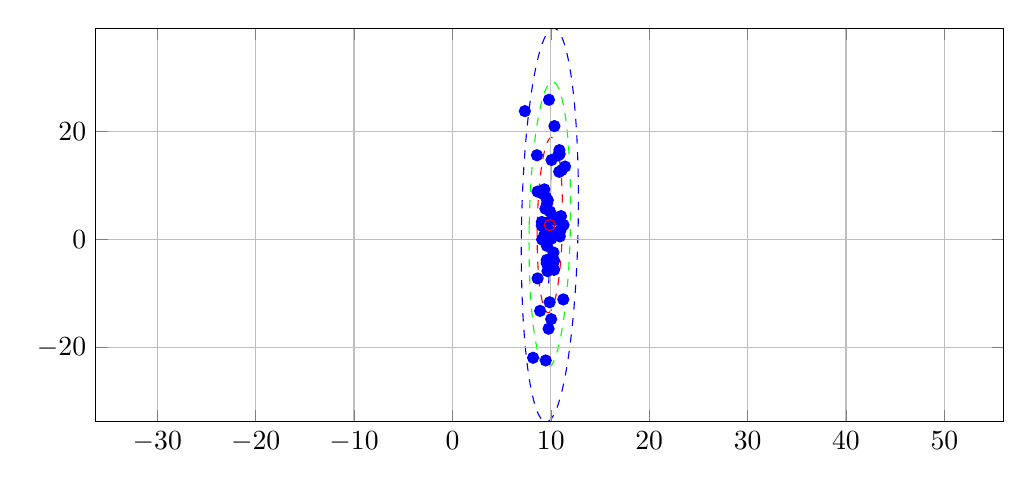
\begin{tikzpicture}

\begin{axis}[%
width=0.95092\figurewidth,
height=\figureheight,
at={(0\figurewidth,0\figureheight)},
scale only axis,
separate axis lines,
every outer x axis line/.append style={black},
every x tick label/.append style={font=\color{black}},
xmin=-36.2393945380367,
xmax=56.0411609525203,
xmajorgrids,
every outer y axis line/.append style={black},
every y tick label/.append style={font=\color{black}},
ymin=-33.7556067659519,
ymax=39.0269603870841,
ymajorgrids,
every outer z axis line/.append style={black},
every z tick label/.append style={font=\color{black}},
zmin=-3.1391283576518,
zmax=4.1391283576518,
zmajorgrids,
view={0}{90},
legend style={legend cell align=left,align=left,draw=black}
]
\addplot [color=blue,only marks,mark=*,mark options={solid}]
  table[row sep=crcr]{%
11.1010479159111	12.7800634320016\\
10.2654188321564	-2.44330361217242\\
9.81404464074737	25.7932697796306\\
9.57906683577328	-4.40975418360709\\
11.2681221143578	-11.1128158936808\\
10.9143071564477	0.543119389031014\\
9.57034854448887	3.05785035897782\\
8.65360615685203	8.82352297722657\\
9.08644963621784	3.21039798364379\\
10.3333266941572	-5.63621147141663\\
8.90741123358919	-13.2302307169266\\
9.61304889167535	-3.86692932017392\\
9.87756482231943	-11.6374394474195\\
9.34022247738409	9.2359479144432\\
9.37552256089639	0.963724228664804\\
9.77368751744229	-16.5300581823224\\
9.44915904634767	5.65594674805797\\
8.65773491758514	-7.22408106838758\\
10.7365892484148	15.5037753365345\\
9.08045112598076	2.52197866672478\\
11.0350392949792	4.29233268833437\\
9.65659262959267	-5.87379336657145\\
9.69211714235693	7.23016403037701\\
11.2955708256022	2.64903038833475\\
10.2610885572818	4.16167132064005\\
9.59772759848202	-1.20273392593171\\
9.17304435319498	8.43380002762061\\
9.48278292283401	-22.3920614159571\\
10.3999093669464	3.65680347857051\\
10.8471342331179	12.4820655515325\\
10.0480109567023	0.0933335437170495\\
9.5070769245243	7.7813357919509\\
10.3354370751796	-3.95495257205553\\
10.6712144486512	3.72748217456145\\
9.57833764771	-3.83976906010968\\
11.4431265027622	13.4502586032493\\
9.63571900872759	6.69942835626373\\
10.8982881506395	15.7592677222661\\
10.9683438281307	1.58240117725563\\
10.0566274263604	1.40690766570213\\
9.91533353408232	5.13304071328229\\
10.8720104110242	16.4839070468213\\
8.19634467273942	-21.9014784705216\\
10.0337400768363	-14.7655395603042\\
10.0691386095133	14.6675318025445\\
10.365586778607	20.9353452902617\\
9.11514030504879	-0.0477382308846677\\
8.58982463397439	15.5381342933836\\
7.36162039439881	23.7019327014232\\
10.545101683344	3.89695984371778\\
};
%\addlegendentry{Daten};

\addplot [color=red,only marks,mark=o,mark options={solid}]
  table[row sep=crcr]{%
9.90088320724178	2.63567681056609\\
};
%\addlegendentry{Mittelwert};

\addplot [color=blue,solid]
  table[row sep=crcr]{%
9.78860895677047	-8.14915322256295\\
10.0131574577131	13.4205068436951\\
};
%\addlegendentry{Eigenvektoren};

\addplot [color=blue,solid]
  table[row sep=crcr]{%
10.7539900504313	2.62679563848486\\
9.04777636405223	2.64455798264732\\
};
%\addlegendentry{};

\addplot3 [color=red,dashed]
 table[row sep=crcr] {%
8.6207245777028	2.64900375685772	1\\
8.62664824802442	3.1573346229872	1\\
8.63382943441054	3.66515067583633	1\\
8.64226104989719	4.17195076227032	1\\
8.65193477349784	4.67723473179059	1\\
8.66284105841522	5.18050393012288	1\\
8.67496914146286	5.68126169132887	1\\
8.68830705368702	6.17901382795547	1\\
8.70284163217864	6.67326911873816	1\\
8.71855853306354	7.16353979337712	1\\
8.73544224565807	7.64934201390756	1\\
8.75347610777629	8.13019635218945	1\\
8.77264232217354	8.60562826304513	1\\
8.79292197411018	9.07516855257819	1\\
8.81429505001814	9.53835384121114	1\\
8.83674045725191	9.99472702098515	1\\
8.8602360449044	10.4438377066704	1\\
8.88475862566727	10.8852426802418	1\\
8.91028399871394	11.3185063282821	1\\
8.93678697358293	11.743201071879	1\\
8.9642413950378	12.1589077885948	1\\
8.99262016887918	12.5652162260889	1\\
9.0218952886835	12.9617254069877	1\\
9.05203786344193	13.3480440246007	1\\
9.08301814607236	13.7237908290933	1\\
9.11480556277611	14.0885950037338	1\\
9.14736874321065	14.4420965308453	1\\
9.18067555144829	14.7839465470991	1\\
9.21469311769046	15.1138076878014	1\\
9.2493878707063	15.4313544198308	1\\
9.2847255709633	15.7362733629008	1\\
9.3206713444177	16.0282635988278	1\\
9.35718971693088	16.3070369685014	1\\
9.39424464927809	16.5723183562624	1\\
9.43179957271479	16.8238459614089	1\\
9.46981742506562	17.061371556562	1\\
9.50826068730025	17.284660732636	1\\
9.54709142056018	17.4934931301722	1\\
9.58627130359975	17.6876626568069	1\\
9.62576167060467	17.8669776906596	1\\
9.66552354935042	18.0312612694408	1\\
9.7055176996632	18.1803512650926	1\\
9.74570465214519	18.3141005437891	1\\
9.78604474712613	18.4323771111399	1\\
9.82649817380259	18.5350642424528	1\\
9.86702500952643	18.6220605979267	1\\
9.90758525920368	18.693280322662	1\\
9.94813889476478	18.7486531313889	1\\
9.98864589466755	18.7881243778303	1\\
10.0290662833935	18.8116551086314	1\\
10.0693601708991	18.8192221018018	1\\
10.109487791982	18.810817889633	1\\
10.1494095455249	18.7864507660675	1\\
10.1890860335769	18.7461447785145	1\\
10.2284781002344	18.6899397041175	1\\
10.2675468702836	18.6178910104992	1\\
10.3062537875651	18.5300698010217	1\\
10.3445606530249	18.426562744616	1\\
10.3824296624115	18.3074719902501	1\\
10.4198234435847	18.1729150661206	1\\
10.456705093397	18.0230247636664	1\\
10.4930382141129	17.8579490065195	1\\
10.5287869493287	17.6778507045224	1\\
10.5639160193588	17.4829075929556	1\\
10.5983907560523	17.2733120571345	1\\
10.6321771370062	17.0492709425481	1\\
10.6652418191416	16.8110053507278	1\\
10.6975521716092	16.5587504210466	1\\
10.729076307992	16.2927550986648	1\\
10.7597831177733	16.0132818888517	1\\
10.7896422970392	15.7206065979242	1\\
10.8186243783846	15.4150180610592	1\\
10.8467007599944	15.0968178572486	1\\
10.8738437338695	14.7663200116767	1\\
10.9000265131717	14.4238506858157	1\\
10.9252232586591	14.0697478555432	1\\
10.9494091041858	13.7043609776015	1\\
10.9725601812422	13.3280506447253	1\\
10.9946536425105	12.9411882297807	1\\
11.0156676844116	12.5441555192649	1\\
11.0355815686233	12.1373443365287	1\\
11.0543756425462	11.7211561550946	1\\
11.0720313586982	11.2960017024507	1\\
11.0885312930192	10.8623005547122	1\\
11.103859162066	10.4204807225505	1\\
11.1179998390824	9.97097822879844	1\\
11.1309393689275	9.51423667814828	1\\
11.1426649818475	9.05070681936742	1\\
11.1531651060781	8.58084610046382	1\\
11.1624293792643	8.10511821724008	1\\
11.1704486586871	7.62399265568162	1\\
11.1772150302858	7.1379442286307	1\\
11.1827218164686	6.64745260720349	1\\
11.1869635827023	6.15300184741255	1\\
11.1899361428757	5.65507991246204	1\\
11.191636563431	5.15417819118691	1\\
11.1920631662583	4.65079101311148	1\\
11.191215530352	4.14541516060581	1\\
11.1890944922265	3.63854937862158	1\\
11.1857021450904	3.13069388249094	1\\
11.1810418367808	2.62234986427446	1\\
11.1751181664591	2.11401899814498	1\\
11.167936980073	1.60620294529585	1\\
11.1595053645864	1.09940285886185	1\\
11.1498316409857	0.594118889341591	1\\
11.1389253560683	0.0908496910093022	1\\
11.1267972730207	-0.409908070196692	1\\
11.1134593607965	-0.907660206823286	1\\
11.0989247823049	-1.40191549760599	1\\
11.08320788142	-1.89218617224494	1\\
11.0663241688255	-2.37798839277538	1\\
11.0482903067073	-2.85884273105727	1\\
11.02912409231	-3.33427464191295	1\\
11.0088444403734	-3.80381493144601	1\\
10.9874713644654	-4.26700022007896	1\\
10.9650259572316	-4.72337339985297	1\\
10.9415303695792	-5.17248408553819	1\\
10.9170077888163	-5.61388905910964	1\\
10.8914824157696	-6.04715270714989	1\\
10.8649794409006	-6.47184745074685	1\\
10.8375250194458	-6.88755416746264	1\\
10.8091462456044	-7.29386260495671	1\\
10.7798711258001	-7.69037178585549	1\\
10.7497285510416	-8.07669040346855	1\\
10.7187482684112	-8.45243720796113	1\\
10.6869608517074	-8.81724138260166	1\\
10.6543976712729	-9.17074290971309	1\\
10.6210908630353	-9.51259292596693	1\\
10.5870732967931	-9.84245406666921	1\\
10.5523785437773	-10.1600007986986	1\\
10.5170408435203	-10.4649197417686	1\\
10.4810950700659	-10.7569099776956	1\\
10.4445766975527	-11.0356833473692	1\\
10.4075217652055	-11.3009647351302	1\\
10.3699668417688	-11.5524923402768	1\\
10.3319489894179	-11.7900179354299	1\\
10.2935057271833	-12.0133071115039	1\\
10.2546749939234	-12.2221395090401	1\\
10.2154951108838	-12.4163090356747	1\\
10.1760047438789	-12.5956240695274	1\\
10.1362428651331	-12.7599076483087	1\\
10.0962487148204	-12.9089976439605	1\\
10.0560617623384	-13.0427469226569	1\\
10.0157216673574	-13.1610234900077	1\\
9.97526824068097	-13.2637106213206	1\\
9.93474140495712	-13.3507069767946	1\\
9.89418115527988	-13.4219267015299	1\\
9.85362751971877	-13.4772995102567	1\\
9.813120519816	-13.5167707566981	1\\
9.77270013109001	-13.5403014874992	1\\
9.73240624358444	-13.5478684806697	1\\
9.69227862250154	-13.5394642685008	1\\
9.65235686895863	-13.5150971449353	1\\
9.61268038090667	-13.4747911573823	1\\
9.57328831424914	-13.4185860829853	1\\
9.53421954419999	-13.3465373893671	1\\
9.49551262691842	-13.2587161798896	1\\
9.45720576145865	-13.1552091234838	1\\
9.41933675207204	-13.0361183691179	1\\
9.38194297089887	-12.9015614449884	1\\
9.34506132108656	-12.7516711425342	1\\
9.3087282003707	-12.5865953853873	1\\
9.27297946515487	-12.4064970833902	1\\
9.23785039512475	-12.2115539718234	1\\
9.20337565843127	-12.0019584360023	1\\
9.16958927747735	-11.777917321416	1\\
9.13652459534193	-11.5396517295957	1\\
9.10421424287432	-11.2873967999144	1\\
9.07269010649153	-11.0214014775326	1\\
9.04198329671021	-10.7419282677195	1\\
9.01212411744435	-10.449252976792	1\\
8.98314203609893	-10.1436644399271	1\\
8.9550656544892	-9.82546423611646	1\\
8.92792268061409	-9.49496639054457	1\\
8.90173990131182	-9.15249706468349	1\\
8.87654315582447	-8.79839423441102	1\\
8.85235731029779	-8.43300735646928	1\\
8.82920623324134	-8.05669702359312	1\\
8.80711277197309	-7.66983460864857	1\\
8.78609873007195	-7.27280189813273	1\\
8.76618484586021	-6.86599071539654	1\\
8.74739077193736	-6.44980253396245	1\\
8.72973505578533	-6.02464808131852	1\\
8.71323512146436	-5.59094693358	1\\
8.69790725241755	-5.14912710141831	1\\
8.68376657540112	-4.69962460766628	1\\
8.67082704555603	-4.24288305701612	1\\
8.65910143263605	-3.77935319823525	1\\
8.64860130840548	-3.30949247933165	1\\
8.63933703521923	-2.83376459610791	1\\
8.63131775579646	-2.35263903454945	1\\
8.62455138419776	-1.86659060749854	1\\
8.619044598015	-1.37609898607132	1\\
8.6148028317813	-0.881648226280372	1\\
8.61183027160781	-0.383726291329869	1\\
8.61012985105254	0.117175429945251	1\\
8.6097032482253	0.620562608020688	1\\
8.61055088413155	1.12593846052635	1\\
8.61267192225701	1.6328042425106	1\\
8.61606426939311	2.14065973864123	1\\
8.6207245777028	2.64900375685771	1\\
};
 %\addlegendentry{1x Standardabweichung};

\addplot3 [color=green,dashed]
 table[row sep=crcr] {%
7.80510974289828	2.65749462263582	1\\
7.81480750283608	3.48969331720274	1\\
7.82656396763916	4.32104920058427	1\\
7.84036753509612	5.15074182489433	1\\
7.85620458275243	5.97795238368272	1\\
7.87405948135406	6.80186451999827	1\\
7.89391461027175	7.62166513203455	1\\
7.91575037489039	8.4365451755632	1\\
7.93954522594657	9.24570046236293	1\\
7.96527568079509	10.0483324538562	1\\
7.99291634658348	10.8436490491702	1\\
8.02243994531171	11.6308653668453	1\\
8.05381734075227	12.4092045194176	1\\
8.08701756720408	13.1778983801135	1\\
8.12200786005196	13.9361883408982	1\\
8.15875368810129	14.6833260611296	1\\
8.19721878765616	15.4185742060812	1\\
8.23736519830727	16.1412071746012	1\\
8.27915330039423	16.8505118151944	1\\
8.32254185410543	17.5457881298158	1\\
8.36748804017672	18.2263499646847	1\\
8.41394750214885	18.8915256874353	1\\
8.46187439014199	19.5406588499368	1\\
8.51122140610396	20.1731088361286	1\\
8.56193985048776	20.7882514942311	1\\
8.61397967031208	21.3854797527077	1\\
8.66728950855761	21.9642042193715	1\\
8.72181675485016	22.5238537630443	1\\
8.7775075973808	23.0638760771936	1\\
8.8343070760116	23.5837382249932	1\\
8.89215913651463	24.0829271652668	1\\
8.95100668589073	24.5609502587983	1\\
9.01079164871342	25.0173357545067	1\\
9.07145502444232	25.4516332550078	1\\
9.13293694564957	25.8634141611021	1\\
9.19517673710173	26.2522720947502	1\\
9.25811297563895	26.6178233001188	1\\
9.32168355079217	26.9597070223019	1\\
9.38582572607868	27.2775858633418	1\\
9.45047620091546	27.5711461152003	1\\
9.51557117308918	27.8400980693508	1\\
9.58104640172133	28.0841763026856	1\\
9.64683727066616	28.3031399394562	1\\
9.71287885227905	28.496772888989	1\\
9.77910597149225	28.6648840589403	1\\
9.84545327013479	28.8073075438818	1\\
9.91185527143312	28.9239027890288	1\\
9.97824644462876	29.014554728951	1\\
10.0445612696493	29.0791739011283	1\\
10.1107343017687	29.1176965342393	1\\
10.1767002361934	29.130084611096	1\\
10.2423939725103	29.1163259061622	1\\
10.307750678933	29.0764339976186	1\\
10.3727058562829	29.0104482539626	1\\
10.437195401642	28.9184337951568	1\\
10.501155671615	28.8004814283628	1\\
10.5645235451374	28.6567075583263	1\\
10.6272364857686	28.4872540724988	1\\
10.6892326034075	28.2922882010126	1\\
10.750450715371	28.0720023516442	1\\
10.8108304067736	27.8266139199316	1\\
10.8703120901494	27.5563650746307	1\\
10.9288370642584	27.2615225187243	1\\
10.9863475720169	26.9423772262184	1\\
11.0427868574971	26.5992441549857	1\\
11.0980992219381	26.2324619359406	1\\
11.1522300787143	25.8423925388512	1\\
11.2051260072053	25.4294209151187	1\\
11.2567348055158	24.9939546178771	1\\
11.3070055419928	24.5364233997873	1\\
11.3558886054887	24.0572787889231	1\\
11.4033357543213	23.5569936431675	1\\
11.4493001638833	23.0360616835595	1\\
11.4937364728518	22.49499700705	1\\
11.5366008279546	21.9343335791515	1\\
11.5778509272483	21.3546247069774	1\\
11.6174460618651	20.7564424931955	1\\
11.6553471561876	20.1403772714314	1\\
11.6915168064115	19.5070370236805	1\\
11.7259193174588	18.8570467803033	1\\
11.7585207382046	18.1910480031957	1\\
11.7892888949826	17.5096979527437	1\\
11.8181934233369	16.8136690391867	1\\
11.8452057979875	16.1036481590298	1\\
11.8702993609819	15.3803360171599	1\\
11.8934493480031	14.6444464353343	1\\
11.9146329128088	13.8967056477255	1\\
11.933829149778	13.1378515842149	1\\
11.9510191145425	12.3686331421456	1\\
11.9661858426825	11.5898094472511	1\\
11.9793143664682	10.8021491044898	1\\
11.9903917296318	10.0064294395244	1\\
11.9994070001532	9.2034357315961	1\\
12.0063512810489	8.39396043854783	1\\
12.011217719152	7.57880241476476	1\\
12.0140015118756	6.75876612280112	1\\
12.0146999119523	5.93466083947292	1\\
12.0133122301458	5.10729985719936	1\\
12.0098398359302	4.27749968138143	1\\
12.0042861561396	3.44607922460969	1\\
11.9966566715853	2.61385899849636	1\\
11.9869589116475	1.78166030392944	1\\
11.9752024468444	0.950304420547916	1\\
11.9613988793874	0.120611796237852	1\\
11.9455618317311	-0.706598762550537	1\\
11.9277069331295	-1.53051089886608	1\\
11.9078518042118	-2.35031151090236	1\\
11.8860160395932	-3.16519155443101	1\\
11.862221188537	-3.97434684123075	1\\
11.8364907336885	-4.77697883272397	1\\
11.8088500679001	-5.57229542803803	1\\
11.7793264691718	-6.35951174571309	1\\
11.7479490737313	-7.13785089828537	1\\
11.7147488472795	-7.90654475898133	1\\
11.6797585544316	-8.66483471976596	1\\
11.6430127263823	-9.41197243999745	1\\
11.6045476268274	-10.147220584949	1\\
11.5644012161763	-10.869853553469	1\\
11.5226131140893	-11.5791581940622	1\\
11.4792245603781	-12.2744345086836	1\\
11.4342783743068	-12.9549963435525	1\\
11.3878189123347	-13.6201720663031	1\\
11.3398920243416	-14.2693052288046	1\\
11.2905450083796	-14.9017552149965	1\\
11.2398265639958	-15.5168978730989	1\\
11.1877867441715	-16.1141261315755	1\\
11.134476905926	-16.6928505982393	1\\
11.0799496596334	-17.2525001419121	1\\
11.0242588171028	-17.7925224560614	1\\
10.967459338472	-18.312384603861	1\\
10.9096072779689	-18.8115735441346	1\\
10.8507597285928	-19.2895966376661	1\\
10.7909747657701	-19.7459821333745	1\\
10.7303113900412	-20.1802796338756	1\\
10.668829468834	-20.5920605399699	1\\
10.6065896773818	-20.980918473618	1\\
10.5436534388446	-21.3464696789866	1\\
10.4800828636914	-21.6883534011697	1\\
10.4159406884049	-22.0062322422096	1\\
10.3512902135681	-22.2997924940681	1\\
10.2861952413944	-22.5687444482186	1\\
10.2207200127622	-22.8128226815534	1\\
10.1549291438174	-23.031786318324	1\\
10.0888875622045	-23.2254192678568	1\\
10.0226604429913	-23.3935304378081	1\\
9.95631314434877	-23.5359539227496	1\\
9.88991114305044	-23.6525491678966	1\\
9.82351996985479	-23.7432011078188	1\\
9.75720514483427	-23.8078202799961	1\\
9.69103211271488	-23.8463429131071	1\\
9.62506617829017	-23.8587309899638	1\\
9.55937244197323	-23.84497228503	1\\
9.49401573555052	-23.8050803764864	1\\
9.42906055820066	-23.7390946328304	1\\
9.36457101284157	-23.6470801740246	1\\
9.30061074286859	-23.5291278072307	1\\
9.23724286934618	-23.3853539371941	1\\
9.174529928715	-23.2159004513667	1\\
9.11253381107604	-23.0209345798804	1\\
9.05131569911251	-22.800648730512	1\\
8.99093600770998	-22.5552602987994	1\\
8.93145432433413	-22.2850114534985	1\\
8.87292935022514	-21.9901688975921	1\\
8.81541884246666	-21.6710236050862	1\\
8.7589795569865	-21.3278905338535	1\\
8.70366719254545	-20.9611083148085	1\\
8.64953633576927	-20.5710389177191	1\\
8.59664040727829	-20.1580672939866	1\\
8.54503160896773	-19.7226009967449	1\\
8.49476087249072	-19.2650697786551	1\\
8.4458778089949	-18.7859251677909	1\\
8.39843066016223	-18.2856400220354	1\\
8.35246625060022	-17.7647080624273	1\\
8.30802994163178	-17.2236433859179	1\\
8.26516558652899	-16.6629799580193	1\\
8.22391548723526	-16.0832710858452	1\\
8.18432035261841	-15.4850888720633	1\\
8.14641925829593	-14.8690236502992	1\\
8.11024960807205	-14.2356834025484	1\\
8.07584709702475	-13.5856931591711	1\\
8.04324567627895	-12.9196943820635	1\\
8.01247751950091	-12.2383443316115	1\\
7.98357299114669	-11.5423154180545	1\\
7.95656061649609	-10.8322945378976	1\\
7.93146705350164	-10.1089823960277	1\\
7.90831706648045	-9.37309281420218	1\\
7.88713350167475	-8.62535202659335	1\\
7.86793726470551	-7.86649796308274	1\\
7.85074729994101	-7.09727952101345	1\\
7.8355805718011	-6.31845582611896	1\\
7.82245204801537	-5.5307954833576	1\\
7.81137468485176	-4.73507581839229	1\\
7.80235941433033	-3.93208211046394	1\\
7.79541513343465	-3.12260681741566	1\\
7.79054869533158	-2.30744879363259	1\\
7.787764902608	-1.48741250166896	1\\
7.78706650253122	-0.66330721834076	1\\
7.7884541843378	0.164053763932801	1\\
7.79192657855335	0.993853939750745	1\\
7.79748025834399	1.82527439652248	1\\
7.80510974289828	2.65749462263581	1\\
};
% \addlegendentry{2x Standardabweichung};

\addplot3 [color=blue,dashed]
 table[row sep=crcr] {%
7.0222422869665	2.66564457553847	1\\
7.03556260477132	3.80870762922134	1\\
7.05171064807642	4.95061304310792	1\\
7.07067048071266	6.09023389441862	1\\
7.09242339161425	7.22644551496129	1\\
7.1169479132844	8.35812660104295	1\\
7.14421984298111	9.48416032006114	1\\
7.17421226660234	10.6034354126829	1\\
7.20689558524701	11.7148472895235	1\\
7.24223754442552	12.8172991212429	1\\
7.28020326589105	13.9097029209839	1\\
7.32075528206017	14.9909806180835	1\\
7.36385357298883	16.060065121999	1\\
7.40945560586719	17.1159013753972	1\\
7.45751637699441	18.1574473953686	1\\
7.50798845619183	19.1836753017388	1\\
7.56082203361086	20.1935723314623	1\\
7.61596496888925	21.1861418380972	1\\
7.67336284260737	22.1604042753746	1\\
7.73295900999359	23.1153981638932	1\\
7.79469465682583	24.0501810399828	1\\
7.85850885747411	24.9638303858023	1\\
7.92433863502677	25.8554445397538	1\\
7.99211902344109	26.7241435863131	1\\
8.06178313165692	27.5690702244005	1\\
8.13326220961012	28.3893906134336	1\\
8.20648571608051	29.1842951962268	1\\
8.28138138830758	29.9529994979269	1\\
8.35787531330512	30.6947449001949	1\\
8.43589200080437	31.4087993898707	1\\
8.51535445775385	32.094458281382	1\\
8.59618426430216	32.7510449121834	1\\
8.67830165118894	33.377911310541	1\\
8.76162557846748	33.974438835002	1\\
8.84607381548138	34.5400387849195	1\\
8.93156302201626	35.0741529814286	1\\
9.01800883054652	35.5762543183017	1\\
9.10532592949587	36.0458472821388	1\\
9.19342814742955	36.4824684413793	1\\
9.28222853809519	36.8856869036528	1\\
9.37163946622818	37.2551047410183	1\\
9.46157269403719	37.5903573826706	1\\
9.55193946828413	37.8911139747279	1\\
9.64265060787294	38.1570777067448	1\\
9.73361659186052	38.3879861046278	1\\
9.82474764780313	38.5836112896662	1\\
9.91595384035096	38.7437602034204	1\\
10.0071451600034	38.8682747982477	1\\
10.0982316119376	38.9570321932756	1\\
10.1891233048226	39.0099447956712	1\\
10.2797305395309	39.0269603870841	1\\
10.369963897661	39.0080621751799	1\\
10.4597343297825	38.9532688102121	1\\
10.5489532433169	38.8626343666167	1\\
10.6375325899682	38.7362482896471	1\\
10.7253849526155	38.5742353071024	1\\
10.8124236315834	38.3767553062363	1\\
10.8985627302041	38.1440031759678	1\\
10.9837172395869	37.8762086145488	1\\
11.067803122512	37.5736359028802	1\\
11.1507373963646	37.2365836436985	1\\
11.2324382150293	36.8653844668905	1\\
11.3128249496618	36.4604047012284	1\\
11.3918182682604	36.0220440128472	1\\
11.4693402139566	35.5507350108222	1\\
11.5453142819492	35.0469428202368	1\\
11.6196654950057	34.5111646231593	1\\
11.6923204774552	33.9439291679851	1\\
11.7632075276019	33.3457962476253	1\\
11.8322566884855	32.7173561470587	1\\
11.8993998169207	32.0592290607922	1\\
11.964570650746	31.3720644808032	1\\
12.0277048742165	30.6565405555698	1\\
12.0887401814761	29.9133634208199	1\\
12.1476163380452	29.1432665026608	1\\
12.2042752402656	28.3470097937756	1\\
12.2586609726413	27.5253791034029	1\\
12.3107198630205	26.6791852818373	1\\
12.3604005355635	25.8092634202186	1\\
12.4076539614447	24.9164720263971	1\\
12.4524335072375	24.0016921776906	1\\
12.4946949809366	23.065826651367	1\\
12.5343966755698	22.1097990337125	1\\
12.5714994103577	21.1345528085629	1\\
12.6059665693805	20.1410504261998	1\\
12.6377641377136	19.1302723535273	1\\
12.6668607349959	18.1032161064706	1\\
12.6932276463988	17.0608952655475	1\\
12.7168388509642	16.0043384755871	1\\
12.7376710472836	14.9345884305814	1\\
12.7557036764944	13.8527008446723	1\\
12.7709189425687	12.7597434102893	1\\
12.7833018298759	11.6567947444657	1\\
12.7928401180012	10.5449433243741	1\\
12.7995243938057	9.42528641313072	1\\
12.8033480607163	8.29892897692909	1\\
12.8043073452353	7.166982594572	1\\
12.8024013006648	6.03056436047728	1\\
12.7976318080406	4.89079578224052	1\\
12.7900035742761	3.74880167384254	1\\
12.7795241275171	2.6057090455937	1\\
12.7662038097122	1.46264599191084	1\\
12.7500557664071	0.320740578024269	1\\
12.7310959337709	-0.818880273286442	1\\
12.7093430228693	-1.95509189382911	1\\
12.6848185011992	-3.08677297991075	1\\
12.6575465715025	-4.21280669892895	1\\
12.6275541478812	-5.3320817915507	1\\
12.5948708292365	-6.44349366839132	1\\
12.559528870058	-7.54594550011074	1\\
12.5215631485925	-8.63834929985168	1\\
12.4810111324234	-9.71962699695131	1\\
12.4379128414947	-10.7887115008668	1\\
12.3923108086164	-11.844547754265	1\\
12.3442500374891	-12.8860937742364	1\\
12.2937779582917	-13.9123216806066	1\\
12.2409443808727	-14.9222187103302	1\\
12.1858014455943	-15.914788216965	1\\
12.1284035718762	-16.8890506542424	1\\
12.06880740449	-17.844044542761	1\\
12.0070717576577	-18.7788274188506	1\\
11.9432575570094	-19.6924767646702	1\\
11.8774277794568	-20.5840909186216	1\\
11.8096473910425	-21.4527899651809	1\\
11.7399832828266	-22.2977166032683	1\\
11.6685042048734	-23.1180369923014	1\\
11.5952806984031	-23.9129415750946	1\\
11.520385026176	-24.6816458767947	1\\
11.4438911011784	-25.4233912790627	1\\
11.3658744136792	-26.1374457687386	1\\
11.2864119567297	-26.8231046602499	1\\
11.2055821501814	-27.4796912910512	1\\
11.1234647632946	-28.1065576894088	1\\
11.0401408360161	-28.7030852138698	1\\
10.9556925990022	-29.2686851637873	1\\
10.8702033924673	-29.8027993602964	1\\
10.783757583937	-30.3049006971695	1\\
10.6964404849877	-30.7744936610067	1\\
10.608338267054	-31.2111148202471	1\\
10.5195378763884	-31.6143332825206	1\\
10.4301269482554	-31.9837511198861	1\\
10.3401937204464	-32.3190037615384	1\\
10.2498269461994	-32.6197603535958	1\\
10.1591158066106	-32.8857240856126	1\\
10.068149822623	-33.1166324834956	1\\
9.97701876668042	-33.312257668534	1\\
9.8858125741326	-33.4724065822883	1\\
9.79462125448015	-33.5969211771155	1\\
9.70353480254591	-33.6856785721435	1\\
9.61264310966095	-33.7385911745391	1\\
9.52203587495266	-33.7556067659519	1\\
9.43180251682254	-33.7367085540477	1\\
9.34203208470106	-33.6819151890799	1\\
9.25281317116663	-33.5912807454845	1\\
9.16423382451534	-33.4648946685149	1\\
9.07638146186806	-33.3028816859702	1\\
8.98934278290016	-33.1054016851042	1\\
8.90320368427947	-32.8726495548356	1\\
8.81804917489664	-32.6048549934166	1\\
8.7339632919716	-32.3022822817481	1\\
8.65102901811898	-31.9652300225663	1\\
8.5693281994543	-31.5940308457583	1\\
8.48894146482172	-31.1890510800963	1\\
8.40994814622311	-30.750690391715	1\\
8.33242620052696	-30.2793813896901	1\\
8.25645213253433	-29.7755891991046	1\\
8.18210091947787	-29.2398110020272	1\\
8.10944593702833	-28.672575546853	1\\
8.03855888688164	-28.0744426264931	1\\
7.96950972599801	-27.4460025259265	1\\
7.90236659756283	-26.78787543966	1\\
7.83719576373756	-26.100710859671	1\\
7.77406154026703	-25.3851869344376	1\\
7.71302623300751	-24.6420097996878	1\\
7.65415007643838	-23.8719128815286	1\\
7.59749117421798	-23.0756561726435	1\\
7.54310544184228	-22.2540254822708	1\\
7.49104655146307	-21.4078316607052	1\\
7.44136587892001	-20.5379097990864	1\\
7.39411245303888	-19.6451184052649	1\\
7.34933290724605	-18.7303385565584	1\\
7.30707143354691	-17.7944730302349	1\\
7.26736973891372	-16.8384454125803	1\\
7.23026700412584	-15.8631991874308	1\\
7.19579984510302	-14.8696968050676	1\\
7.16400227676997	-13.8589187323952	1\\
7.13490567948765	-12.8318624853385	1\\
7.10853876808471	-11.7895416444154	1\\
7.08492756351939	-10.7329848544549	1\\
7.06409536719998	-9.66323480944921	1\\
7.04606273798915	-8.58134722354012	1\\
7.03084747191481	-7.4883897891571	1\\
7.01846458460763	-6.38544112333352	1\\
7.00892629648237	-5.27358970324192	1\\
7.00224202067785	-4.15393279199855	1\\
6.99841835376726	-3.02757535579694	1\\
6.99745906924823	-1.89562897343985	1\\
6.99936511381876	-0.759210739345125	1\\
7.00413460644297	0.380557838891654	1\\
7.01176284020747	1.52255194728963	1\\
7.0222422869665	2.66564457553847	1\\
};
% \addlegendentry{3x Standardabweichung};

\end{axis}
\end{tikzpicture}%
					\caption{PCA 2}
					\label{fig:pca2}
				\end{subfigure}	
				\\
				\begin{subfigure}{0.45\textwidth}
					\centering
					% This file was created by matlab2tikz.
% Minimal pgfplots version: 1.3
%
%The latest updates can be retrieved from
%  http://www.mathworks.com/matlabcentral/fileexchange/22022-matlab2tikz
%where you can also make suggestions and rate matlab2tikz.
%
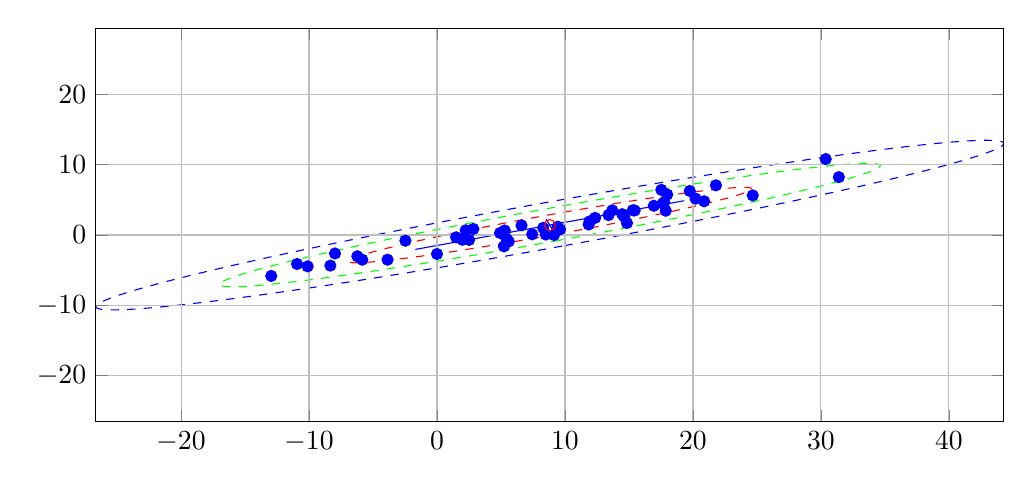
\begin{tikzpicture}

\begin{axis}[%
width=0.95092\figurewidth,
height=\figureheight,
at={(0\figurewidth,0\figureheight)},
scale only axis,
separate axis lines,
every outer x axis line/.append style={black},
every x tick label/.append style={font=\color{black}},
xmin=-26.656869505919,
xmax=44.2809467595858,
xmajorgrids,
every outer y axis line/.append style={black},
every y tick label/.append style={font=\color{black}},
ymin=-26.5653116066968,
ymax=29.3840305769029,
ymajorgrids,
every outer z axis line/.append style={black},
every z tick label/.append style={font=\color{black}},
zmin=-0.199366777294997,
zmax=1.199366777295,
zmajorgrids,
view={0}{90},
legend style={legend cell align=left,align=left,draw=black}
]
\addplot [color=blue,only marks,mark=*,mark options={solid}]
  table[row sep=crcr]{%
5.44472978269709	-0.577289933813434\\
5.22805993100385	-1.61349419707251\\
7.43870466825692	0.100336381683103\\
17.9867387828379	5.75031853523774\\
8.29352813628289	1.01157140895627\\
30.3730913354772	10.7926493491835\\
6.60318793578978	1.37177345507569\\
2.84143991718599	0.856429263381885\\
15.4451966610762	3.48756508581657\\
12.3531091903292	2.42635440824064\\
14.6252626849383	2.60421079873865\\
-10.9387635929438	-4.12081253325755\\
8.49997477137822	0.0670570937670636\\
-8.33525474571426	-4.35064291141613\\
11.8533876174123	1.48679170628117\\
17.6498906665636	4.46330552161421\\
21.7957902617132	7.0546388980878\\
17.5296775004699	6.41643212919879\\
14.8407754035302	1.6965304618198\\
17.7543759736931	4.67306011027556\\
9.43338702977036	1.17591462388934\\
9.61498587566128	0.803017651447581\\
20.2044747193525	5.16472265010514\\
20.8728389278498	4.78998728434885\\
5.29169777657604	0.638628144502255\\
-7.97279740485603	-2.62333345417865\\
-12.953226877787	-5.82144860077072\\
-6.22578573194761	-3.02044631926593\\
-0.000719054247699802	-2.70057294974776\\
14.4711755856635	2.95810012862123\\
2.24159088802308	0.66132907044002\\
9.14665607150171	-0.00170154930304056\\
13.6939096941233	3.49902389303887\\
-3.86210853860879	-3.51063256772806\\
1.49750180459497	-0.33175520459092\\
2.50618354370613	-0.698436589563464\\
1.98210580859646	-0.683896919629093\\
5.60750581178614	-0.921637027767139\\
17.8717947302458	3.45046983270511\\
4.92528953683873	0.284565540228405\\
16.9431050270731	4.15461037217091\\
13.4032700587016	2.82966763240154\\
11.9185584382323	1.93433790779544\\
19.7503240575992	6.25365189610861\\
31.401608574977	8.22601915643582\\
24.6733281566119	5.62610157558818\\
-5.84033827180256	-3.51074860674999\\
15.2991185966086	3.51413691363539\\
-2.46844330524427	-0.811528812240311\\
-10.1079630699076	-4.45695644857533\\
};
%\addlegendentry{Daten};

\addplot [color=red,only marks,mark=o,mark options={solid}]
  table[row sep=crcr]{%
8.81203862683338	1.40935948510302\\
};
%\addlegendentry{Mittelwert};

\addplot [color=blue,solid]
  table[row sep=crcr]{%
19.3195667747376	4.86956046177552\\
-1.69548952107083	-2.05084149156947\\
};
%\addlegendentry{Eigenvektoren};

\addplot [color=blue,solid]
  table[row sep=crcr]{%
8.52125195291776	2.29238598610764\\
9.10282530074901	0.526332984098401\\
};
%\addlegendentry{};

\addplot3 [color=red,dashed]
 table[row sep=crcr] {%
9.24838850837491	0.0843038904880058	1\\
8.75290623626761	-0.0781370761031068	1\\
8.25748232069066	-0.239110063175945	1\\
7.76260568523548	-0.398456209826773	1\\
7.26876471339409	-0.556018260646939	1\\
6.77644676658354	-0.71164072091498	1\\
6.28613770317907	-0.86517001005114	1\\
5.79832139903053	-1.01645461318286	1\\
5.31347926993535	-1.16534523067165	1\\
4.83208979653923	-1.31169492545384	1\\
4.35462805213357	-1.45535926804969	1\\
3.88156523381544	-1.59619647909787	1\\
3.41336819747295	-1.73406756927455	1\\
2.95049899705486	-1.86883647645911	1\\
2.49341442857911	-2.00037020001099	1\\
2.04256557933028	-2.12853893202533	1\\
1.59839738269096	-2.25321618543761	1\\
1.16134817904615	-2.37427891885119	1\\
0.731849283194245	-2.49160765796427	1\\
0.310324558691434	-2.6050866134766	1\\
-0.1028100004505	-2.7146037953596	1\\
-0.507146680300021	-2.82005112337689	1\\
-0.90228644937028	-2.92132453374655	1\\
-1.28783935241501	-3.01832408183942	1\\
-1.66342489526726	-3.11095404081243	1\\
-2.02867242034124	-3.19912299607943	1\\
-2.38322147242656	-3.28274393552634	1\\
-2.72672215441404	-3.3617343353816	1\\
-3.05883547260191	-3.43601624165717	1\\
-3.37923367124163	-3.50551634707974	1\\
-3.68760055599329	-3.57016606343609	1\\
-3.98363180597123	-3.62990158926143	1\\
-4.267035274072	-3.68466397280374	1\\
-4.53753127528831	-3.73439917020201	1\\
-4.79485286272433	-3.77905809882099	1\\
-5.03874609104008	-3.81859668568989	1\\
-5.26897026706479	-3.85297591099701	1\\
-5.48529818733202	-3.88216184659764	1\\
-5.68751636230207	-3.90612568949699	1\\
-5.87542522705033	-3.92484379027531	1\\
-6.04883933821381	-3.93829767642699	1\\
-6.20758755700132	-3.94647407059073	1\\
-6.35151321808683	-3.94936490365261	1\\
-6.48047428421921	-3.94696732270942	1\\
-6.59434348639584	-3.9392836938841	1\\
-6.69300844946177	-3.92632159999064	1\\
-6.77637180301041	-3.90809383305077	1\\
-6.84435127747639	-3.8846183816698	1\\
-6.89687978532568	-3.85591841328402	1\\
-6.93390548726287	-3.82202225129724	1\\
-6.95539184339033	-3.782963347129	1\\
-6.96131764926862	-3.73878024720209	1\\
-6.95167705684277	-3.68951655490182	1\\
-6.9264795802136	-3.63522088754484	1\\
-6.88575008624841	-3.57594682839963	1\\
-6.8295287700404	-3.51175287380631	1\\
-6.75787111524099	-3.44270237544784	1\\
-6.67084783930414	-3.36886347782954	1\\
-6.56854482369675	-3.29030905102867	1\\
-6.45106302914403	-3.2071166187805	1\\
-6.31851839599346	-3.11936828197171	1\\
-6.17104172979564	-3.02715063761675	1\\
-6.00877857221504	-2.93055469339702	1\\
-5.83188905739793	-2.8296757778473	1\\
-5.64054775393929	-2.72461344627798	1\\
-5.43494349260473	-2.61547138252598	1\\
-5.21527917997729	-2.50235729663136	1\\
-4.98177159821312	-2.38538281854045	1\\
-4.73465119110372	-2.26466338794064	1\\
-4.4741618366557	-2.14031814033529	1\\
-4.20056060641264	-2.01246978947141	1\\
-3.91411751175651	-1.88124450623597	1\\
-3.61511523743904	-1.74677179414052	1\\
-3.303848862606	-1.6091843615168	1\\
-2.98062556958971	-1.46861799054969	1\\
-2.64576434075715	-1.32521140327653	1\\
-2.2995956437129	-1.17910612468529	1\\
-1.94246110516748	-1.03044634304643	1\\
-1.57471317379306	-0.879378767616515	1\\
-1.19671477239917	-0.726052483853882	1\\
-0.808838939771675	-0.570618806289301	1\\
-0.411468462528564	-0.413231129196789	1\\
-0.00499549735576466	-0.254044775211997	1\\
0.410178816004187	-0.0932168420475015	1\\
0.833644750628593	0.0690939525436509	1\\
1.26498439676565	0.232727427403223	1\\
1.70377207426088	0.397522096047232	1\\
2.14957475265208	0.563315326033631	1\\
2.60195247851809	0.729943499460884	1\\
3.0604588096597	0.897242174439078	1\\
3.52464125568421	1.06504624737423	1\\
3.99404172455882	1.23319011590557	1\\
4.46819697469216	1.40150784233513	1\\
4.94663907209782	1.56983331738816	1\\
5.42889585218864	1.73800042414296	1\\
5.91449138574628	1.90584320196824	1\\
6.40294644860574	2.07319601030617	1\\
6.89377899459188	2.23989369213968	1\\
7.38650463124077	2.40577173698246	1\\
7.88063709783649	2.57066644323094	1\\
8.37568874529186	2.73441507971804	1\\
8.87117101739915	2.89685604630915	1\\
9.3665949329761	3.05782903338198	1\\
9.86147156843128	3.21717518003281	1\\
10.3553125402727	3.37473723085298	1\\
10.8476304870832	3.53035969112102	1\\
11.3379395504877	3.68388898025718	1\\
11.8257558546362	3.8351735833889	1\\
12.3105979837314	3.98406420087769	1\\
12.7919874571275	4.13041389565988	1\\
13.2694492015332	4.27407823825573	1\\
13.7425120198513	4.41491544930391	1\\
14.2107090561938	4.55278653948059	1\\
14.6735782566119	4.68755544666515	1\\
15.1306628250877	4.81908917021704	1\\
15.5815116743365	4.94725790223137	1\\
16.0256798709758	5.07193515564365	1\\
16.4627290746206	5.19299788905723	1\\
16.8922279704725	5.31032662817031	1\\
17.3137526949753	5.42380558368265	1\\
17.7268872541173	5.53332276556564	1\\
18.1312239339668	5.63877009358293	1\\
18.526363703037	5.74004350395259	1\\
18.9119166060818	5.83704305204546	1\\
19.287502148934	5.92967301101847	1\\
19.652749674008	6.01784196628548	1\\
20.0072987260933	6.10146290573238	1\\
20.3507994080808	6.18045330558764	1\\
20.6829127262687	6.25473521186321	1\\
21.0033109249084	6.32423531728578	1\\
21.3116778096601	6.38888503364213	1\\
21.607709059638	6.44862055946747	1\\
21.8911125277388	6.50338294300979	1\\
22.1616085289551	6.55311814040805	1\\
22.4189301163911	6.59777706902703	1\\
22.6628233447068	6.63731565589593	1\\
22.8930475207316	6.67169488120306	1\\
23.1093754409988	6.70088081680368	1\\
23.3115936159688	6.72484465970303	1\\
23.4995024807171	6.74356276048135	1\\
23.6729165918806	6.75701664663304	1\\
23.8316648106681	6.76519304079677	1\\
23.9755904717536	6.76808387385865	1\\
24.104551537886	6.76568629291547	1\\
24.2184207400626	6.75800266409014	1\\
24.3170857031285	6.74504057019668	1\\
24.4004490566772	6.72681280325681	1\\
24.4684285311432	6.70333735187584	1\\
24.5209570389924	6.67463738349006	1\\
24.5579827409296	6.64074122150328	1\\
24.5794690970571	6.60168231733505	1\\
24.5853949029354	6.55749921740813	1\\
24.5757543105095	6.50823552510787	1\\
24.5505568338804	6.45393985775089	1\\
24.5098273399152	6.39466579860567	1\\
24.4536060237072	6.33047184401235	1\\
24.3819483689078	6.26142134565388	1\\
24.2949250929709	6.18758244803558	1\\
24.1926220773635	6.10902802123471	1\\
24.0751402828108	6.02583558898654	1\\
23.9425956496602	5.93808725217776	1\\
23.7951189834624	5.84586960782279	1\\
23.6328558258818	5.74927366360307	1\\
23.4559663110647	5.64839474805335	1\\
23.2646250076061	5.54333241648402	1\\
23.0590207462715	5.43419035273203	1\\
22.8393564336441	5.3210762668374	1\\
22.6058488518799	5.2041017887465	1\\
22.3587284447705	5.08338235814668	1\\
22.0982390903225	4.95903711054133	1\\
21.8246378600794	4.83118875967745	1\\
21.5381947654233	4.69996347644202	1\\
21.2391924911058	4.56549076434657	1\\
20.9279261162728	4.42790333172285	1\\
20.6047028232565	4.28733696075573	1\\
20.2698415944239	4.14393037348258	1\\
19.9236728973797	3.99782509489134	1\\
19.5665383588343	3.84916531325248	1\\
19.1987904274598	3.69809773782256	1\\
18.8207920260659	3.54477145405992	1\\
18.4329161934384	3.38933777649534	1\\
18.0355457161953	3.23195009940283	1\\
17.6290727510225	3.07276374541804	1\\
17.2138984376626	2.91193581225355	1\\
16.7904325030382	2.74962501766239	1\\
16.3590928569011	2.58599154280282	1\\
15.9203051794059	2.42119687415881	1\\
15.4745025010147	2.25540364417241	1\\
15.0221247751487	2.08877547074516	1\\
14.5636184440071	1.92147679576696	1\\
14.0994359979826	1.75367272283182	1\\
13.630035529108	1.58552885430047	1\\
13.1558802789746	1.41721112787092	1\\
12.677438181569	1.24888565281788	1\\
12.1951814014781	1.08071854606308	1\\
11.7095858679205	0.912875768237808	1\\
11.221130805061	0.745522959899876	1\\
10.7302982590749	0.578825278066364	1\\
10.237572622426	0.412947233223584	1\\
9.74344015583029	0.248052526975103	1\\
9.24838850837491	0.0843038904880071	1\\
};
% \addlegendentry{1x Standardabweichung};

\addplot3 [color=green,dashed]
 table[row sep=crcr] {%
9.52639580242301	-0.759915704624156	1\\
8.71523179979542	-1.02585108126304	1\\
7.90416333381847	-1.28938319907945	1\\
7.09399083114662	-1.55025198368973	1\\
6.28551383422669	-1.80819998909853	1\\
5.47953021224603	-2.06297265176696	1\\
4.67683537373195	-2.31431854183604	1\\
3.87822148157954	-2.56198961125762	1\\
3.08447667128253	-2.80574143858789	1\\
2.29638427313872	-3.04533347020177	1\\
1.51472203919752	-3.28052925769037	1\\
0.740261375712606	-3.51109669120695	1\\
-0.0262334181429278	-3.7368082285314	1\\
-0.784005904547586	-3.95744111962684	1\\
-1.53230825354427	-4.1727776264671	1\\
-2.27040198105815	-4.38260523791783	1\\
-2.99755867769131	-4.58671687945931	1\\
-3.71306072757486	-4.78491111754404	1\\
-4.41620201656919	-4.97699235838731	1\\
-5.10628862911333	-5.16277104099465	1\\
-5.78263953303586	-5.34206382423567	1\\
-6.44458725165144	-5.51469376777959	1\\
-7.09147852247973	-5.68049050671399	1\\
-7.72267494193654	-5.83929041967444	1\\
-8.33755359536114	-5.99093679031897	1\\
-8.93550767175778	-6.13527996198826	1\\
-9.51594706264495	-6.27217748539864	1\\
-10.0782989444211	-6.40149425922232	1\\
-10.6220083436726	-6.52310266341615	1\\
-11.1465386848651	-6.63688268516716	1\\
-11.6513723198792	-6.7427220373307	1\\
-12.1360110388664	-6.84051626924433	1\\
-12.5999765619222	-6.93016886980799	1\\
-13.0428110110907	-7.01159136272881	1\\
-13.4640773622345	-7.08470339383654	1\\
-13.8633598763252	-7.14943281038339	1\\
-14.2402645097273	-7.20571573225012	1\\
-14.5944193030719	-7.25349661498795	1\\
-14.9254747483356	-7.29272830463428	1\\
-15.2331041337628	-7.32337208424794	1\\
-15.5170038662904	-7.34539771211811	1\\
-15.7768937711583	-7.35878345160926	1\\
-16.0125173684072	-7.3635160926126	1\\
-16.2236421259937	-7.35959096458284	1\\
-16.4100596892715	-7.34701194114746	1\\
-16.5715860866122	-7.32579143628391	1\\
-16.7080619109628	-7.2959503920685	1\\
-16.8193524771617	-7.25751825800912	1\\
-16.9053479548563	-7.21053296198211	1\\
-16.9659634768926	-7.15504087280206	1\\
-17.0011392230683	-7.09109675446135	1\\
-17.0108404791689	-7.0187637120847	1\\
-16.9950576712259	-6.93811312965207	1\\
-16.9538063749652	-6.84922459955127	1\\
-16.8871273004358	-6.75218584402984	1\\
-16.7950862518342	-6.64709262862388	1\\
-16.677774062563	-6.53404866764891	1\\
-16.5353065055897	-6.41316552184647	1\\
-16.3678241791927	-6.28456248828706	1\\
-16.1754923682079	-6.14836648263837	1\\
-15.9585008809122	-6.00471191391483	1\\
-15.7170638617058	-5.85374055183215	1\\
-15.4514195797777	-5.69560138689771	1\\
-15.1618301939624	-5.53045048337493	1\\
-14.8485814940213	-5.35845082526666	1\\
-14.5119826186021	-5.17977215546971	1\\
-14.152365750157	-4.99459080825901	1\\
-13.7700857871179	-4.80308953526706	1\\
-13.3655199936551	-4.60545732513005	1\\
-12.939067627363	-4.40188921697898	1\\
-12.4911495452409	-4.19258610795952	1\\
-12.0222077883581	-3.97775455497079	1\\
-11.5327051456125	-3.75760657081867	1\\
-11.0231246970142	-3.53235941498472	1\\
-10.4939693369435	-3.30223537921734	1\\
-9.94576127785518	-3.06746156815662	1\\
-9.37904153491755	-2.82826967520949	1\\
-8.794369392096	-2.5848957538963	1\\
-8.19232185020716	-2.33757998489449	1\\
-7.57349305748882	-2.08656643900928	1\\
-6.93849372324726	-1.83210283630523	1\\
-6.28795051516097	-1.57444030163643	1\\
-5.62250544083533	-1.31383311681663	1\\
-4.94281521421852	-1.05053846967377	1\\
-4.24955060750422	-0.784816200236618	1\\
-3.54339578916041	-0.516928544304078	1\\
-2.82504764873769	-0.247139874650089	1\\
-2.09521510912344	0.0242835598803852	1\\
-1.35461842692049	0.297073897126815	1\\
-0.603988481640872	0.570961925960707	1\\
0.155933945584088	0.845677351964512	1\\
0.924398903065248	1.12094906417955	1\\
1.70064800866748	1.39650540265983	1\\
2.48391519824126	1.6720744265676	1\\
3.27342748163545	1.94738418254609	1\\
4.06840570554534	2.22216297310472	1\\
4.86806532244278	2.49613962475164	1\\
5.67161716482998	2.76904375560928	1\\
6.47826822405252	3.04060604224862	1\\
7.28722243290308	3.31055848547882	1\\
8.09768145124375	3.5786346748302	1\\
8.90884545387135	3.84457005146908	1\\
9.71991391984828	4.10810216928549	1\\
10.5300864225201	4.36897095389577	1\\
11.3385634194401	4.62691895930457	1\\
12.1445470414207	4.881691621973	1\\
12.9472418799348	5.13303751204208	1\\
13.7458557720872	5.38070858146366	1\\
14.5396005823842	5.62446040879393	1\\
15.327692980528	5.86405244040781	1\\
16.1093552144692	6.0992482278964	1\\
16.8838158779542	6.32981566141299	1\\
17.6503106718097	6.55552719873744	1\\
18.4080831582143	6.77616008983288	1\\
19.156385507211	6.99149659667314	1\\
19.8944792347249	7.20132420812387	1\\
20.6216359313581	7.40543584966535	1\\
21.3371379812416	7.60363008775008	1\\
22.040279270236	7.79571132859335	1\\
22.7303658827801	7.98149001120069	1\\
23.4067167867026	8.16078279444172	1\\
24.0686645053182	8.33341273798563	1\\
24.7155557761465	8.49920947692003	1\\
25.3467521956033	8.65800938988048	1\\
25.9616308490279	8.80965576052501	1\\
26.5595849254246	8.95399893219431	1\\
27.1400243163117	9.09089645560468	1\\
27.7023761980879	9.22021322942836	1\\
28.2460855973394	9.3418216336222	1\\
28.7706159385318	9.4556016553732	1\\
29.2754495735459	9.56144100753674	1\\
29.7600882925331	9.65923523945037	1\\
30.224053815589	9.74888784001403	1\\
30.6668882647575	9.83031033293485	1\\
31.0881546159013	9.90342236404258	1\\
31.487437129992	9.96815178058943	1\\
31.8643417633941	10.0244347024562	1\\
32.2184965567387	10.072215585194	1\\
32.5495520020024	10.1114472748403	1\\
32.8571813874295	10.142091054454	1\\
33.1410811199572	10.1641166823241	1\\
33.4009710248251	10.1775024218153	1\\
33.6365946220739	10.1822350628186	1\\
33.8477193796604	10.1783099347889	1\\
34.0341369429383	10.1657309113535	1\\
34.1956633402789	10.14451040649	1\\
34.3321391646296	10.1146693622745	1\\
34.4434297308285	10.0762372282152	1\\
34.5294252085231	10.0292519321882	1\\
34.5900407305593	9.97375984300811	1\\
34.6252164767351	9.90981572466739	1\\
34.6349177328357	9.83748268229074	1\\
34.6191349248926	9.75683209985812	1\\
34.5778836286319	9.66794356975731	1\\
34.5112045541026	9.57090481423589	1\\
34.419163505501	9.46581159882992	1\\
34.3018513162297	9.35276763785495	1\\
34.1593837592564	9.23188449205252	1\\
33.9919014328595	9.1032814584931	1\\
33.7995696218747	8.96708545284441	1\\
33.582578134579	8.82343088412087	1\\
33.3411411153726	8.67245952203819	1\\
33.0754968334444	8.51432035710376	1\\
32.7859074476292	8.34916945358097	1\\
32.4726587476881	8.17716979547271	1\\
32.1360598722689	7.99849112567575	1\\
31.7764430038238	7.81330977846506	1\\
31.3941630407846	7.6218085054731	1\\
30.9895972473219	7.4241762953361	1\\
30.5631448810298	7.22060818718503	1\\
30.1152267989077	7.01130507816556	1\\
29.6462850420249	6.79647352517684	1\\
29.1567823992793	6.57632554102471	1\\
28.6472019506809	6.35107838519077	1\\
28.1180465906103	6.12095434942339	1\\
27.5698385315219	5.88618053836267	1\\
27.0031187885843	5.64698864541553	1\\
26.4184466457628	5.40361472410234	1\\
25.8163991038739	5.15629895510053	1\\
25.1975703111556	4.90528540921532	1\\
24.562570976914	4.65082180651127	1\\
23.9120277688278	4.39315927184247	1\\
23.2465826945021	4.13255208702268	1\\
22.5668924678853	3.86925743987982	1\\
21.873627861171	3.60353517044266	1\\
21.1674730428272	3.33564751451012	1\\
20.4491249024045	3.06585884485614	1\\
19.7192923627902	2.79443541032566	1\\
18.9786956805873	2.52164507307923	1\\
18.2280657353076	2.24775704424534	1\\
17.4681433080827	1.97304161824153	1\\
16.6996783506015	1.69776990602649	1\\
15.9234292449993	1.42221356754621	1\\
15.1401620554255	1.14664454363845	1\\
14.3506497720313	0.871334787659955	1\\
13.5556715481214	0.59655599710133	1\\
12.756011931224	0.322579345454407	1\\
11.9524600888368	0.0496752145967623	1\\
11.1458090296143	-0.221887072042572	1\\
10.3368548207637	-0.49183951527278	1\\
9.52639580242302	-0.759915704624154	1\\
};
% \addlegendentry{2x Standardabweichung};

\addplot3 [color=blue,dashed]
 table[row sep=crcr] {%
9.7932409525288	-1.57023942419164	1\\
8.67907001242219	-1.93551385406963	1\\
7.5650302962845	-2.29748729779332	1\\
6.45222122681593	-2.65580253127532	1\\
5.34174101221696	-3.01010594064011	1\\
4.23468556238952	-3.36004787119823	1\\
3.13214740740614	-3.7052829725132	1\\
2.03521461931477	-4.04547053922077	1\\
0.944969738342934	-4.38027484726395	1\\
-0.137511295438696	-4.7093654852121	1\\
-1.2111602039393	-5.03241768033717	1\\
-2.27491742530939	-5.34911261912513	1\\
-3.32773315960044	-5.65913776190644	1\\
-4.3685684047907	-5.96218715129497	1\\
-5.39639598215471	-6.25796171413099	1\\
-6.41020154996474	-6.54616955663027	1\\
-7.40898460452361	-6.82652625244802	1\\
-8.39175946754099	-7.09875512337334	1\\
-9.35755625887895	-7.36258751237722	1\\
-10.3054218537065	-7.61776304874459	1\\
-11.2344208231187	-7.86402990502875	1\\
-12.1436363572922	-8.10114504557473	1\\
-13.0321711702656	-8.32887446636605	1\\
-13.8991483854528	-8.54699342595851	1\\
-14.7437124010136	-8.7552866672728	1\\
-15.5650297342302	-8.9535486300273	1\\
-16.3622898440536	-9.14158365360123	1\\
-17.1347059310098	-9.31920617012806	1\\
-17.8815157136758	-9.4862408876286	1\\
-18.6019821809596	-9.64252296300303	1\\
-19.2953943194409	-9.78789816471112	1\\
-19.9610678150557	-9.92222302498014	1\\
-20.5983457284317	-10.0453649813902	1\\
-21.2065991432077	-10.1572025076976	1\\
-21.7852277866988	-10.2576252337659	1\\
-22.3336606222925	-10.3465340544889	1\\
-22.8513564129931	-10.4238412275946	1\\
-23.3378042555574	-10.4894704602364	1\\
-23.7925240846943	-10.5433569842854	1\\
-24.2150671468316	-10.585447620248	1\\
-24.605016442981	-10.6157008297482	1\\
-24.9619871402665	-10.6340867565208	1\\
-25.2856269517074	-10.6405872558758	1\\
-25.5756164838833	-10.6351959126052	1\\
-25.8316695521369	-10.6179180473138	1\\
-26.0535334630034	-10.5887707111687	1\\
-26.2409892635888	-10.5477826690717	1\\
-26.3938519576496	-10.4949943712719	1\\
-26.5119706881623	-10.4304579134458	1\\
-26.5952288862004	-10.3542369852858	1\\
-26.6435443859743	-10.2664068076458	1\\
-26.656869505919	-10.1670540583072	1\\
-26.6351910957498	-10.0562767864386	1\\
-26.5785305494404	-9.93418431583304	1\\
-26.4869437841092	-9.80089713701858	1\\
-26.3605211848362	-9.65654678834877	1\\
-26.1993875154636	-9.50127572619012	1\\
-26.0037017954694	-9.33523718433487	1\\
-25.7736571430335	-9.15859502277777	1\\
-25.5094805844545	-8.971523566006	1\\
-25.2114328301012	-8.77420743096198	1\\
-24.8798080171234	-8.56684134484873	1\\
-24.5149334191739	-8.34962995295766	1\\
-24.1171691234291	-8.12278761670828	1\\
-23.6869076752263	-7.88653820209949	1\\
-23.2245736906686	-7.64111485878075	1\\
-22.7306234375806	-7.38675978996161	1\\
-22.2055443852268	-7.12372401338633	1\\
-21.6498547232383	-6.8522671136097	1\\
-21.0641028502222	-6.57265698581841	1\\
-20.4488668325586	-6.28516957145084	1\\
-19.8047538339184	-5.99008858587621	1\\
-19.1323995160667	-5.68770523840171	1\\
-18.4324674115409	-5.37831794488412	1\\
-17.7056482688242	-5.06223203322936	1\\
-16.9526593706607	-4.73975944207072	1\\
-16.1742438261834	-4.41121841292308	1\\
-15.3711698375553	-4.07693317611698	1\\
-14.5442299418471	-3.73723363082239	1\\
-13.694240228898	-3.3924550194781	1\\
-12.8220395359343	-3.04293759694788	1\\
-11.9284886197379	-2.68902629473002	1\\
-11.0144693071833	-2.33107038055157	1\\
-10.0808836249811	-1.96942311368329	1\\
-9.12865290948654	-1.60444139631538	1\\
-8.15871689745156	-1.2364854213381	1\\
-7.17203279861828	-0.865918316874888	1\\
-6.16957435106839	-0.493105787918743	1\\
-5.15233086026136	-0.118415755425536	1\\
-4.12130622270934	0.257782006779527	1\\
-3.07751793525246	0.635116236924066	1\\
-2.02199609091237	1.01321455167903	1\\
-0.955782362314732	1.39170381365613	1\\
0.120071026315896	1.77021049964936	1\\
1.20450233757425	2.1483610692573	1\\
2.29644136868113	2.52578233352242	1\\
3.39481050764421	2.90210182322351	1\\
4.49852579673105	3.27694815645785	1\\
5.60649800220449	3.64995140515027	1\\
6.71763368926482	4.02074346012754	1\\
7.83083630113796	4.38895839439768	1\\
8.94500724124457	4.75423282427567	1\\
10.0590469573823	5.11620626799935	1\\
11.1718560268508	5.47452150148136	1\\
12.2823362414498	5.82882491084615	1\\
13.3893916912772	6.17876684140426	1\\
14.4919298462606	6.52400194271924	1\\
15.588862634352	6.86418950942681	1\\
16.6791075153238	7.19899381746999	1\\
17.7615885491055	7.52808445541814	1\\
18.835237457606	7.8511366505432	1\\
19.8989946789762	8.16783158933117	1\\
20.9518104132672	8.47785673211248	1\\
21.9926456584575	8.78090612150101	1\\
23.0204732358215	9.07668068433703	1\\
24.0342788036315	9.3648885268363	1\\
25.0330618581904	9.64524522265406	1\\
26.0158367212077	9.91747409357938	1\\
26.9816335125457	10.1813064825833	1\\
27.9294991073732	10.4364820189506	1\\
28.8584980767855	10.6827488752348	1\\
29.7677136109589	10.9198640157808	1\\
30.6562484239324	11.1475934365721	1\\
31.5232256391195	11.3657123961645	1\\
32.3677896546804	11.5740056374788	1\\
33.189106987897	11.7722676002333	1\\
33.9863670977204	11.9603026238073	1\\
34.7587831846765	12.1379251403341	1\\
35.5055929673426	12.3049598578346	1\\
36.2260594346263	12.4612419332091	1\\
36.9194715731076	12.6066171349172	1\\
37.5851450687225	12.7409419951862	1\\
38.2224229820985	12.8640839515963	1\\
38.8306763968745	12.9759214779036	1\\
39.4093050403656	13.076344203972	1\\
39.9577378759592	13.165253024695	1\\
40.4754336666598	13.2425601978006	1\\
40.9618815092241	13.3081894304425	1\\
41.4166013383611	13.3620759544914	1\\
41.8391444004983	13.404166590454	1\\
42.2290936966478	13.4344197999542	1\\
42.5860643939332	13.4528057267268	1\\
42.9097042053741	13.4593062260818	1\\
43.1996937375501	13.4539148828112	1\\
43.4557468058036	13.4366370175198	1\\
43.6776107166702	13.4074896813747	1\\
43.8650665172555	13.3665016392778	1\\
44.0179292113164	13.3137133414779	1\\
44.136047941829	13.2491768836518	1\\
44.2193061398671	13.1729559554919	1\\
44.2676216396411	13.0851257778519	1\\
44.2809467595858	12.9857730285133	1\\
44.2592683494166	12.8749957566447	1\\
44.2026078031072	12.7529032860391	1\\
44.111021037776	12.6196161072246	1\\
43.9845984385029	12.4752657585548	1\\
43.8234647691304	12.3199946963962	1\\
43.6277790491361	12.1539561545409	1\\
43.3977343967003	11.9773139929838	1\\
43.1335578381213	11.790242536212	1\\
42.835510083768	11.592926401168	1\\
42.5038852707902	11.3855603150548	1\\
42.1390106728407	11.1683489231637	1\\
41.7412463770959	10.9415065869143	1\\
41.310984928893	10.7052571723055	1\\
40.8486509443354	10.4598338289868	1\\
40.3547006912474	10.2054787601677	1\\
39.8296216388936	9.94244298359238	1\\
39.2739319769051	9.67098608381574	1\\
38.688180103889	9.39137595602445	1\\
38.0729440862253	9.10388854165688	1\\
37.4288310875852	8.80880755608225	1\\
36.7564767697335	8.50642420860776	1\\
36.0565446652077	8.19703691509017	1\\
35.329725522491	7.8809510034354	1\\
34.5767366243275	7.55847841227676	1\\
33.7983210798501	7.22993738312913	1\\
32.9952470912221	6.89565214632302	1\\
32.1683071955138	6.55595260102843	1\\
31.3183174825648	6.21117398968414	1\\
30.4461167896011	5.86165656715393	1\\
29.5525658734047	5.50774526493607	1\\
28.6385465608501	5.14978935075762	1\\
27.7049608786479	4.78814208388935	1\\
26.7527301631533	4.42316036652143	1\\
25.7827941511183	4.05520439154415	1\\
24.7961100522851	3.68463728708094	1\\
23.7936516047352	3.31182475812479	1\\
22.7764081139281	2.93713472563158	1\\
21.7453834763761	2.56093696342652	1\\
20.7015951889192	2.18360273328198	1\\
19.6460733445792	1.80550441852701	1\\
18.5798596159815	1.42701515654992	1\\
17.5040062273509	1.04850847055668	1\\
16.4195749160925	0.670357900948747	1\\
15.3276358849857	0.292936636683629	1\\
14.2292667460226	-0.0833828530174632	1\\
13.1255514569357	-0.458229186251797	1\\
12.0175792514623	-0.831232434944227	1\\
10.9064435644019	-1.2020244899215	1\\
9.79324095252881	-1.57023942419163	1\\
};
% \addlegendentry{3x Standardabweichung};

\end{axis}
\end{tikzpicture}%
					\caption{PCA 3}
					\label{fig:pca3}
				\end{subfigure}
				\qquad
				\begin{subfigure}{0.45\textwidth}
					\centering
					% This file was created by matlab2tikz.
% Minimal pgfplots version: 1.3
%
%The latest updates can be retrieved from
%  http://www.mathworks.com/matlabcentral/fileexchange/22022-matlab2tikz
%where you can also make suggestions and rate matlab2tikz.
%
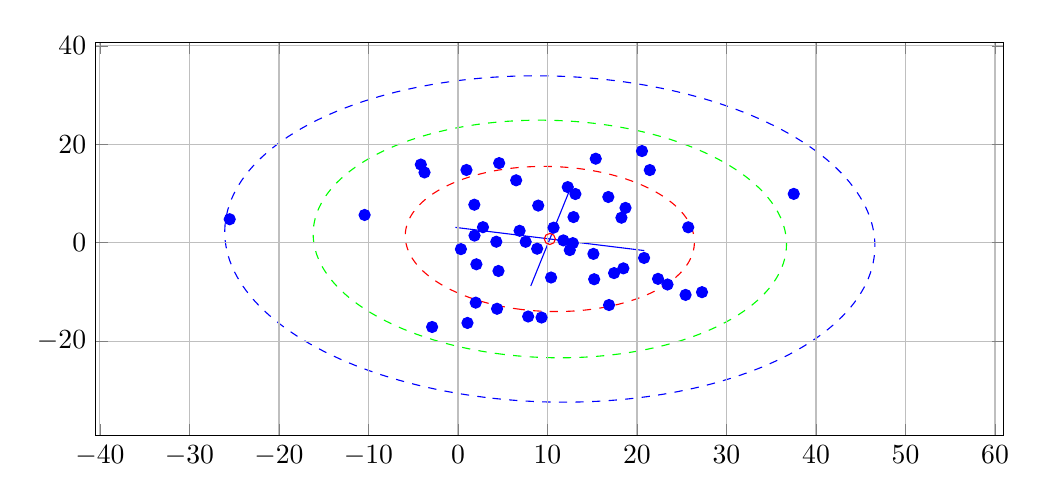
\begin{tikzpicture}

\begin{axis}[%
width=0.95092\figurewidth,
height=\figureheight,
at={(0\figurewidth,0\figureheight)},
scale only axis,
separate axis lines,
every outer x axis line/.append style={black},
every x tick label/.append style={font=\color{black}},
xmin=-40.4536270780981,
xmax=60.9778657644377,
xmajorgrids,
every outer y axis line/.append style={black},
every y tick label/.append style={font=\color{black}},
ymin=-39.2534336936029,
ymax=40.7465663063971,
ymajorgrids,
every outer z axis line/.append style={black},
every z tick label/.append style={font=\color{black}},
zmin=0,
zmax=1,
zmajorgrids,
view={0}{90},
legend style={legend cell align=left,align=left,draw=black}
]
\addplot [color=blue,only marks,mark=*,mark options={solid}]
  table[row sep=crcr]{%
18.7156557243306	7.06059506234169\\
12.265244553888	11.2921146138128\\
4.36673989443474	-13.4349783131208\\
1.82777791632296	7.71055922213634\\
11.7734404598447	0.460780474919601\\
8.96672983503264	7.53328570799877\\
0.950094104596426	14.7678425960038\\
2.0565735372081	-4.3941237685512\\
15.3912820294882	17.0593483426331\\
15.2166391689867	-7.43393573397202\\
6.88599604829554	2.40831693453769\\
18.2612770354213	5.06955631164682\\
6.5005934102686	12.6682307672474\\
8.84497310049439	-1.23146333398642\\
22.3482171829568	-7.35874145579186\\
4.60079013541161	16.1661411698876\\
-10.4295541608974	5.62642928190036\\
-2.88880154150336	-17.1367787710994\\
12.9084875627763	5.19922422174947\\
7.84207756680738	-15.0058679799209\\
37.5134027656672	9.9091598831421\\
-4.15076615934147	15.8716658481553\\
7.56130990949062	0.17222125136134\\
10.4025070078518	-7.08393356847147\\
-3.73829429801884	14.2692984951034\\
20.7918731483707	-3.10703299406317\\
17.4393115949833	-6.18471951493772\\
25.4286065009815	-10.6177054406154\\
16.875221467436	-12.6764802945527\\
-25.501683039025	4.75779186692215\\
0.329468473982711	-1.31746313840677\\
13.1179042820021	9.88484408845746\\
1.8493105713285	1.43306034580109\\
12.8337045148214	-0.0968647255023156\\
9.33762135282234	-15.2146551394431\\
4.52503215581019	-5.75463907445961\\
10.6805624790237	3.04429626048291\\
15.1297373621053	-2.28145137621409\\
21.4309605165656	14.7504684048415\\
1.06054882586093	-16.3143051877386\\
4.28227561922965	0.188020609456912\\
2.79356977649472	3.1457557491049\\
18.4789601029615	-5.2235759714857\\
25.7262685395206	3.12002827504684\\
20.5572101931724	18.6126749449529\\
23.4101376686318	-8.50388785955973\\
12.4927537344373	-1.50881516799212\\
1.98294160728703	-12.1908054304414\\
16.7974785394543	9.27937514727138\\
27.2637983804176	-10.0605463167353\\
};
%\addlegendentry{Daten};

\addplot [color=red,only marks,mark=o,mark options={solid}]
  table[row sep=crcr]{%
10.2621193431698	0.746566306397075\\
};
%\addlegendentry{Mittelwert};

\addplot [color=blue,solid]
  table[row sep=crcr]{%
20.8124782305383	-1.60765541163705\\
-0.288239544198733	3.1007880244312\\
};
%\addlegendentry{Eigenvektoren};

\addplot [color=blue,solid]
  table[row sep=crcr]{%
12.3912707076002	10.2882806012721\\
8.13296797873937	-8.79514798847796\\
};
%\addlegendentry{};

\addplot3 [color=red,dashed]
 table[row sep=crcr] {%
7.06714849686902	-13.5715791787701	1\\
6.57143925735671	-13.4535490028944	1\\
6.07937227350788	-13.3215050276091	1\\
5.59143315602764	-13.175577564376	1\\
5.10810344191532	-13.0159106259832	1\\
4.62986011924567	-12.8426617844221	1\\
4.15717515643913	-12.6560020153828	1\\
3.69051503648606	-12.4561155295216	1\\
3.23034029658427	-12.2431995906674	1\\
2.77710507364449	-12.0174643211463	1\\
2.33125665611202	-11.7791324944158	1\\
1.893235042547	-11.528439315215	1\\
1.46347250739906	-11.2656321874449	1\\
1.04239317440452	-10.9909704700118	1\\
0.630412598027522	-10.7047252208703	1\\
0.22793735335793	-10.4071789295226	1\\
-0.164635365129191	-10.098625238235	1\\
-0.546918135556572	-9.77936865224868	1\\
-0.918533690983359	-9.44972423926973	1\\
-1.27911529172204	-9.11001731853528	1\\
-1.62830708726622	-8.76058313976279	1\\
-1.96576446747214	-8.401766552299	1\\
-2.29115440264727	-8.03392166479528	1\\
-2.60415577221037	-7.65741149574517	1\\
-2.90445968159882	-7.27260761522887	1\\
-3.19176976711017	-6.87988977821852	1\\
-3.46580248837739	-6.47964554980587	1\\
-3.72628740818896	-6.07226992272227	1\\
-3.97296745937776	-5.6581649275286	1\\
-4.20559919851529	-5.23773923585963	1\\
-4.42395304616101	-4.81140775711441	1\\
-4.62781351342947	-4.37959122899084	1\\
-4.81697941465185	-3.94271580226835	1\\
-4.99126406592191	-3.50121262024849	1\\
-5.1504954693305	-3.0555173932686	1\\
-5.29451648270667	-2.60606996870827	1\\
-5.42318497469812	-2.15331389691309	1\\
-5.53637396503757	-1.69769599346402	1\\
-5.63397174985703	-1.23966589822435	1\\
-5.71588201192601	-0.779675631599443	1\\
-5.78202391570499	-0.318179148447158	1\\
-5.83233218712035	0.144368109920784	1\\
-5.866757177982	0.607509665204379	1\\
-5.88526491498013	1.07078845260432	1\\
-5.8878371332128	1.53374727188977	1\\
-5.87447129421115	1.99592923859979	1\\
-5.8451805884446	2.45687823493313	1\\
-5.79999392230343	2.91613935988148	1\\
-5.73895588957168	3.37325937816176	1\\
-5.66212672741844	3.82778716750471	1\\
-5.56958225695105	4.27927416385805	1\\
-5.46141380838884	4.72727480406506	1\\
-5.33772813093121	5.17134696558164	1\\
-5.19864728740905	5.61105240279784	1\\
-5.04430853382348	6.04595717953342	1\\
-4.87486418389075	6.47563209728043	1\\
-4.69048145872699	6.89965311877033	1\\
-4.49134232182112	7.3176017864476	1\\
-4.27764329945892	7.72906563543678	1\\
-4.04959528677526	8.13363860059556	1\\
-3.8074233396261	8.53092141725201	1\\
-3.55136645248549	8.92052201523063	1\\
-3.28167732258692	9.30205590577826	1\\
-2.99862210054162	9.67514656100808	1\\
-2.70248012768011	10.0394257854872	1\\
-2.39354366037593	10.3945340796009	1\\
-2.07211758162396	10.7401209943357	1\\
-1.73851910015769	11.0758454771301	1\\
-1.39307743740249	11.4013762084519	1\\
-1.03613350257383	11.7163919287712	1\\
-0.668039556241022	12.0205817556042	1\\
-0.289158862688565	12.3136454903173	1\\
0.100134668581816	12.5952939143863	1\\
0.499456851854745	12.8652490748204	1\\
0.908413604346066	13.1232445584683	1\\
1.32660133511503	13.369025754936	1\\
1.75360734335978	13.6023501078559	1\\
2.18901022570324	13.8229873542614	1\\
2.63238029206737	14.0307197518281	1\\
3.08327998972537	14.2253422937594	1\\
3.54126433511344	14.4066629111035	1\\
4.00588135297582	14.5745026623023	1\\
4.47667252240974	14.7286959097847	1\\
4.9531732293703	14.8690904834316	1\\
5.43491322518834	14.9955478307488	1\\
5.92141709064918	15.1079431536018	1\\
6.41220470517391	15.2061655313766	1\\
6.90679172064052	15.290118030445	1\\
7.40469003937696	15.359717799826	1\\
7.90540829585461	15.4148961529502	1\\
8.4084523416068	15.4555986354447	1\\
8.9133257328936	15.4817850788735	1\\
9.41953022063191	15.4934296403783	1\\
9.92656624210716	15.4905208281829	1\\
10.4339334139813	15.4730615129337	1\\
10.941131026111	15.4410689248669	1\\
11.4476585356876	15.3945746368045	1\\
11.9530160612132	15.3336245329955	1\\
12.4567048758224	15.2582787638338	1\\
12.9582278994665	15.1686116864968	1\\
13.4570901894706	15.0647117915642	1\\
13.9527994289829	14.9466816156885	1\\
14.4448664128317	14.8146376404032	1\\
14.932805530312	14.6687101771701	1\\
15.4161352444243	14.5090432387773	1\\
15.8943785670939	14.3357943972163	1\\
16.3670635299005	14.149134628177	1\\
16.8337236498535	13.9492481423157	1\\
17.2938983897553	13.7363322034616	1\\
17.7471336126951	13.5105969339404	1\\
18.1929820302276	13.27226510721	1\\
18.6310036437926	13.0215719280091	1\\
19.0607661789405	12.7587648002391	1\\
19.4818455119351	12.4841030828059	1\\
19.8938260883121	12.1978578336644	1\\
20.2963013329817	11.9003115423167	1\\
20.6888740514688	11.5917578510291	1\\
21.0711568218962	11.2725012650428	1\\
21.442772377323	10.9428568520639	1\\
21.8033539780616	10.6031499313294	1\\
22.1525457736058	10.2537157525569	1\\
22.4900031538117	9.89489916509316	1\\
22.8153930889869	9.52705427758945	1\\
23.12839445855	9.15054410853932	1\\
23.4286983679384	8.76574022802302	1\\
23.7160084534498	8.37302239101268	1\\
23.990041174717	7.97277816260002	1\\
24.2505260945286	7.56540253551643	1\\
24.4972061457174	7.15129754032275	1\\
24.7298378848549	6.73087184865378	1\\
24.9481917325006	6.30454036990856	1\\
25.1520521997691	5.872723841785	1\\
25.3412181009914	5.43584841506251	1\\
25.5155027522615	4.99434523304265	1\\
25.6747341556701	4.54865000606276	1\\
25.8187551690463	4.09920258150242	1\\
25.9474236610377	3.64644650970724	1\\
26.0606126513772	3.19082860625818	1\\
26.1582104361966	2.7327985110185	1\\
26.2401206982656	2.2728082443936	1\\
26.3062626020446	1.81131176124131	1\\
26.3565708734599	1.34876450287337	1\\
26.3909958643216	0.885622947589779	1\\
26.4095036013197	0.422344160189841	1\\
26.4120758195524	-0.0406146590956049	1\\
26.3987099805507	-0.502796625805631	1\\
26.3694192747842	-0.963745622138976	1\\
26.324232608643	-1.42300674708732	1\\
26.2631945759113	-1.88012676536761	1\\
26.186365413758	-2.33465455471056	1\\
26.0938209432906	-2.78614155106389	1\\
25.9856524947284	-3.23414219127091	1\\
25.8619668172708	-3.67821435278748	1\\
25.7228859737486	-4.11791979000368	1\\
25.5685472201631	-4.55282456673927	1\\
25.3991028702304	-4.98249948448628	1\\
25.2147201450666	-5.40652050597618	1\\
25.0155810081607	-5.82446917365344	1\\
24.8018819857985	-6.23593302264263	1\\
24.5738339731149	-6.6405059878014	1\\
24.3316620259657	-7.03778880445785	1\\
24.0756051388251	-7.42738940243647	1\\
23.8059160089265	-7.8089232929841	1\\
23.5228607868812	-8.18201394821392	1\\
23.2267188140197	-8.546293172693	1\\
22.9177823467155	-8.90140146680674	1\\
22.5963562679636	-9.24698838154159	1\\
22.2627577864973	-9.58271286433592	1\\
21.9173161237421	-9.90824359565773	1\\
21.5603721889134	-10.223259315977	1\\
21.1922782425806	-10.5274491428101	1\\
20.8133975490282	-10.8205128775232	1\\
20.4241040177578	-11.1021613015921	1\\
20.0247818344849	-11.3721164620262	1\\
19.6158250819935	-11.6301119456742	1\\
19.1976373512246	-11.8758931421418	1\\
18.7706313429798	-12.1092174950618	1\\
18.3352284606364	-12.3298547414672	1\\
17.8918583942722	-12.5375871390339	1\\
17.4409586966142	-12.7322096809652	1\\
16.9829743512262	-12.9135302983094	1\\
16.5183573333638	-13.0813700495081	1\\
16.0475661639299	-13.2355632969906	1\\
15.5710654569693	-13.3759578706375	1\\
15.0893254611513	-13.5024152179546	1\\
14.6028215956904	-13.6148105408076	1\\
14.1120339811657	-13.7130329185825	1\\
13.6174469656991	-13.7969854176508	1\\
13.1195486469626	-13.8665851870319	1\\
12.618830390485	-13.921763540156	1\\
12.1157863447328	-13.9624660226505	1\\
11.610912953446	-13.9886524660793	1\\
11.1047084657077	-14.0002970275841	1\\
10.5976724442324	-13.9973882153887	1\\
10.0903052723583	-13.9799289001395	1\\
9.58310766022862	-13.9479363120728	1\\
9.07658015065196	-13.9014420240104	1\\
8.57122262512644	-13.8404919202014	1\\
8.06753381051718	-13.7651461510396	1\\
7.56601078687314	-13.6754790737026	1\\
7.06714849686903	-13.5715791787701	1\\
};
% \addlegendentry{1x Standardabweichung};

\addplot3 [color=green,dashed]
 table[row sep=crcr] {%
5.03156825010748	-22.6939579177217	1\\
4.22003267457185	-22.5007283406331	1\\
3.41445990910817	-22.2845564904078	1\\
2.61564495677796	-22.0456557025631	1\\
1.82437615149708	-21.784261743334	1\\
1.04143438004531	-21.5006325769996	1\\
0.267592311425345	-21.1950481113042	1\\
-0.496386365668155	-20.8678099212217	1\\
-1.24974769651717	-20.5192409513378	1\\
-1.99174820444256	-20.1496851971425	1\\
-2.72165562452582	-19.7595073655483	1\\
-3.43874962626611	-19.3490925149682	1\\
-4.14232252445952	-18.9188456753096	1\\
-4.83167997759893	-18.4691914482591	1\\
-5.50614167310521	-18.0005735882513	1\\
-6.16504199871365	-17.513454564537	1\\
-6.80773069935288	-17.0083151047822	1\\
-7.4335735188681	-16.4856537206474	1\\
-8.0419528259554	-15.945986215817	1\\
-8.63226822368917	-15.3898451769635	1\\
-9.2039371420415	-14.8177794481485	1\\
-9.75639541280842	-14.23035358918	1\\
-10.2890978263758	-13.62814731846	1\\
-10.8015186697753	-13.0117549408724	1\\
-11.2931522454999	-12.3817847612761	1\\
-11.7635133705659	-11.738858484181	1\\
-12.2121378553303	-11.0836106002012	1\\
-12.6385829615898	-10.4166877598892	1\\
-13.0424278395098	-9.73874813556971	1\\
-13.4232739429525	-9.05046077180338	1\\
-13.7807454227941	-8.35250492512027	1\\
-14.1144894978418	-7.64556939367585	1\\
-14.4241768029872	-6.93035183749027	1\\
-14.7095017142489	-6.20755808994223	1\\
-14.9701826503873	-5.47790146119662	1\\
-15.2059623507908	-4.7421020342535	1\\
-15.4166081293612	-4.00088595431311	1\\
-15.6019121041464	-3.25498471215826	1\\
-15.7616914024956	-2.50513442226121	1\\
-15.8957883415315	-1.75207509632755	1\\
-16.0040705837651	-0.996549912994043	1\\
-16.0864312676963	-0.239304484400964	1\\
-16.1427891132737	0.51891387963701	1\\
-16.1730885021078	1.27735690913539	1\\
-16.1772995323599	2.03527611239199	1\\
-16.1554180482517	2.79192351465789	1\\
-16.107465644166	3.5465523962982	1\\
-16.0334896433364	4.29841802971421	1\\
-15.9335630511444	5.04677841429955	1\\
-15.8077844830724	5.79089500870529	1\\
-15.6562780673814	6.53003345969104	1\\
-15.4791933226123	7.26346432684294	1\\
-15.2767050100284	7.99046380244329	1\\
-15.0490129611475	8.71031442578139	1\\
-14.7963418805323	9.42230579120062	1\\
-14.518941124034	10.1257352491831	1\\
-14.2170844527083	10.8199085997798	1\\
-13.8910697626461	11.5041407777023	1\\
-13.5412187909863	12.1777565283993	1\\
-13.1678767984	12.8400910744515	1\\
-12.7714122283597	13.4904907716266	1\\
-12.3522163435302	14.1283137539472	1\\
-11.9107028396398	14.7529305671349	1\\
-11.4473074372122	15.3637247898062	1\\
-10.9624874515632	15.9600936418053	1\\
-10.4567213414856	16.5414485790757	1\\
-9.93050823706829	17.1072158744823	1\\
-9.38436744711472	17.6568371840103	1\\
-8.81883794664824	18.1897700977839	1\\
-8.23447784500859	18.7054886753589	1\\
-7.63186383506546	19.2034839647627	1\\
-7.01159062409218	19.6832645047683	1\\
-6.37427034686149	20.1443568099075	1\\
-5.72053196154239	20.5863058377433	1\\
-5.05102062899444	21.0086754379424	1\\
-4.36639707607175	21.4110487827028	1\\
-3.66733694356545	21.7930287781123	1\\
-2.95453011942779	22.1542384560324	1\\
-2.22868005793596	22.4943213461204	1\\
-1.49050308546774	22.8129418276225	1\\
-0.740727693573762	23.1097854605909	1\\
0.0199061799556777	23.3845592961983	1\\
0.790647881319819	23.6369921658428	1\\
1.57073678151221	23.8668349487586	1\\
2.35940302696961	24.0738608178683	1\\
3.15586829932461	24.2578654636335	1\\
3.95934658351179	24.4186672956841	1\\
4.76904494346977	24.5561076220257	1\\
5.58416430467336	24.6700508056495	1\\
6.40390024272357	24.7603843983898	1\\
7.22744377721751	24.8270192518967	1\\
8.0539821701142	24.8698896056148	1\\
8.88269972780907	24.8889531516806	1\\
9.71277860612496	24.8841910766758	1\\
10.5433996174256	24.8556080801935	1\\
11.3737430390549	24.8032323702003	1\\
12.2029894223044	24.7271156351987	1\\
13.0303204011098	24.6273329932163	1\\
13.85491949968	24.503982917674	1\\
14.6759729382597	24.357187140204	1\\
15.4926704362321	24.1870905305158	1\\
16.3042060117677	23.9938609534272	1\\
17.1097787772314	23.7776891032019	1\\
17.9085937295616	23.5387883153573	1\\
18.6998625348425	23.2773943561282	1\\
19.4828043062943	22.9937651897938	1\\
20.2566463749142	22.6881807240983	1\\
21.0206250520077	22.3609425340158	1\\
21.7739863828568	22.012373564132	1\\
22.5159868907821	21.6428178099367	1\\
23.2458943108654	21.2526399783425	1\\
23.9629883126057	20.8422251277623	1\\
24.6665612107991	20.4119782881038	1\\
25.3559186639385	19.9623240610532	1\\
26.0303803594448	19.4937062010454	1\\
26.6892806850532	19.0065871773312	1\\
27.3319693856925	18.5014477175764	1\\
27.9578122052077	17.9787863334416	1\\
28.566191512295	17.4391188286112	1\\
29.1565069100288	16.8829777897577	1\\
29.7281758283811	16.3109120609426	1\\
30.280634099148	15.7234862019741	1\\
30.8133365127154	15.1212799312541	1\\
31.3257573561149	14.5048875536666	1\\
31.8173909318394	13.8749173740703	1\\
32.2877520569055	13.2319910969752	1\\
32.7363765416699	12.5767432129954	1\\
33.1628216479294	11.9098203726833	1\\
33.5666665258494	11.2318807483639	1\\
33.9475126292921	10.5435933845975	1\\
34.3049841091337	9.84563753791443	1\\
34.6387281841814	9.13870200647001	1\\
34.9484154893268	8.42348445028443	1\\
35.2337404005885	7.7006907027364	1\\
35.4944213367269	6.97103407399079	1\\
35.7302010371304	6.23523464704765	1\\
35.9408468157008	5.49401856710727	1\\
36.126150790486	4.74811732495243	1\\
36.2859300888352	3.99826703505535	1\\
36.4200270278711	3.2452077091217	1\\
36.5283092701047	2.4896825257882	1\\
36.6106699540359	1.73243709719512	1\\
36.6670277996133	0.974218733157153	1\\
36.6973271884474	0.215775703658782	1\\
36.7015382186995	-0.542143499597812	1\\
36.6796567345912	-1.29879090186373	1\\
36.6317043305056	-2.05341978350404	1\\
36.557728329676	-2.80528541692004	1\\
36.457801737484	-3.5536458015054	1\\
36.3320231694119	-4.29776239591114	1\\
36.180516753721	-5.03690084689688	1\\
36.0034320089519	-5.77033171404878	1\\
35.800943696368	-6.49733118964913	1\\
35.5732516474871	-7.21718181298722	1\\
35.3205805668719	-7.92917317840647	1\\
35.0431798103736	-8.63260263638891	1\\
34.7413231390479	-9.32677598698561	1\\
34.4153084489857	-10.0110081649081	1\\
34.0654574773259	-10.6846239156051	1\\
33.6921154847396	-11.3469584616574	1\\
33.2956509146993	-11.9973581588324	1\\
32.8764550298698	-12.635181141153	1\\
32.4349415259794	-13.2597979543408	1\\
31.9715461235518	-13.8705921770121	1\\
31.4867261379028	-14.4669610290111	1\\
30.9809600278252	-15.0483159662816	1\\
30.4547469234079	-15.6140832616882	1\\
29.9086061334543	-16.1637045712162	1\\
29.3430766329878	-16.6966374849897	1\\
28.7587165313482	-17.2123560625647	1\\
28.1561025214051	-17.7103513519685	1\\
27.5358293104318	-18.1901318919742	1\\
26.8985090332011	-18.6512241971133	1\\
26.244770647882	-19.0931732249491	1\\
25.575259315334	-19.5155428251483	1\\
24.8906357624113	-19.9179161699086	1\\
24.1915756299051	-20.2998961653181	1\\
23.4787688057674	-20.6611058432382	1\\
22.7529187442756	-21.0011887333262	1\\
22.0147417718073	-21.3198092148283	1\\
21.2649663799134	-21.6166528477967	1\\
20.5043325063839	-21.8914266834042	1\\
19.7335908050198	-22.1438595530486	1\\
18.9535019048274	-22.3737023359645	1\\
18.16483565937	-22.5807282050741	1\\
17.368370387015	-22.7647328508394	1\\
16.5648921028278	-22.92553468289	1\\
15.7551937428698	-23.0629750092316	1\\
14.9400743816662	-23.1769181928554	1\\
14.120338443616	-23.2672517855957	1\\
13.2967949091221	-23.3338866391026	1\\
12.4702565162254	-23.3767569928206	1\\
11.6415389585305	-23.3958205388864	1\\
10.8114600802146	-23.3910584638816	1\\
9.980839068914	-23.3624754673993	1\\
9.15049564728468	-23.3100997574062	1\\
8.32124926403524	-23.2339830224046	1\\
7.49391828522983	-23.1342003804222	1\\
6.66931918665961	-23.0108503048799	1\\
5.84826574807987	-22.8640545274099	1\\
5.03156825010748	-22.6939579177217	1\\
};
% \addlegendentry{2x Standardabweichung};

\addplot3 [color=blue,dashed]
 table[row sep=crcr] {%
3.0777176565131	-31.4500681926418	1\\
1.96303634398499	-31.1846585111671	1\\
0.856545224416635	-30.8877365659008	1\\
-0.240663729045231	-30.5595953829553	1\\
-1.32750770363119	-30.2005587980611	1\\
-2.40291411555458	-29.8109811369805	1\\
-3.46582166852223	-29.3912468658307	1\\
-4.51518140110575	-28.9417702116622	1\\
-5.54995772193981	-28.4629947536666	1\\
-6.56912943172581	-27.9553929854178	1\\
-7.57169073103226	-27.4194658485776	1\\
-8.55665221289747	-26.8557422385266	1\\
-9.52304183925466	-26.2647784824089	1\\
-10.4699059002163	-25.6471577901039	1\\
-11.3963099552704	-25.0034896786685	1\\
-12.3013397554608	-24.3344093708178	1\\
-13.1841021456403	-23.6405771680365	1\\
-14.0437259459069	-22.9226777989415	1\\
-14.8793628113536	-22.1814197435371	1\\
-15.6901880692816	-21.4175345340306	1\\
-16.4754015330536	-20.6317760328989	1\\
-17.2342282917807	-19.824919688917	1\\
-17.9659194750665	-18.9977617718832	1\\
-18.669752992051	-18.1511185867978	1\\
-19.345034244028	-17.285825668268	1\\
-19.9910968099294	-16.4027369559362	1\\
-20.6073031040027	-15.502723951745	1\\
-21.1930450050313	-14.5866748598696	1\\
-21.7477444564761	-13.6554937101677	1\\
-22.2708540369484	-12.7100994660113	1\\
-22.761857500448	-11.7514251173804	1\\
-23.220270285836	-10.780416760115	1\\
-23.645639995038	-9.79803266223258	1\\
-24.0375468395066	-8.80524231823294	1\\
-24.3956040545019	-7.80302549232462	1\\
-24.7194582807812	-6.7923712515157	1\\
-25.0087899133228	-5.77427698952407	1\\
-25.2633134167367	-4.74974744247032	1\\
-25.482777607054	-3.71979369732443	1\\
-25.6669658996152	-2.68543219408506	1\\
-25.8156965228128	-1.64768372267591	1\\
-25.9288226974781	-0.607572415549373	1\\
-26.0062327817347	0.433875263008578	1\\
-26.0478503811753	1.47563152987471	1\\
-26.0536344242537	2.51666829738637	1\\
-26.0235792028177	3.55595818793994	1\\
-25.9577143777423	4.59247554788841	1\\
-25.8561049496579	5.62519745973778	1\\
-25.7188511948025	6.65310475164308	1\\
-25.5460885660614	7.67518300320795	1\\
-25.3379875592912	8.6904235465951	1\\
-25.0947535450612	9.69782446195967	1\\
-24.8166265659776	10.6963915662232	1\\
-24.50388109979	11.6851393942123	1\\
-24.1568257885152	12.6630921711936	1\\
-23.7758031338451	13.6292847758459	1\\
-23.3611891591384	14.5827636927184	1\\
-22.9133930383311	15.5225879532349	1\\
-22.4328566921314	16.4478300643167	1\\
-21.9200543518972	17.357576923706	1\\
-21.3754920916268	18.2509307210876	1\\
-20.7997073285255	19.1270098241194	1\\
-20.1932682926389	19.9849496484971	1\\
-19.5567734660793	20.8239035111943	1\\
-18.8908509923956	21.6430434660367	1\\
-18.1961580566714	22.4415611207847	1\\
-17.473380236963	23.2186684349194	1\\
-16.7232308277165	23.9735984973431	1\\
-15.9464501358321	24.7056062832279	1\\
-15.1438047500709	25.4139693892654	1\\
-14.316086784524	26.0979887465919	1\\
-13.4641130968919	26.7569893106842	1\\
-12.5887244823442	27.3903207275477	1\\
-11.6907848437566	27.9973579755369	1\\
-10.7711803391427	28.5775019821767	1\\
-9.83081850712337	29.1301802153741	1\\
-8.87062737129559	29.6548472484386	1\\
-7.89155452438516	30.1509852983523	1\\
-6.89456619308704	30.6181047367594	1\\
-5.8806462845164	31.0557445731704	1\\
-4.85079541521095	31.4634729099035	1\\
-3.80602992364327	31.840887368316	1\\
-2.7473808672175	32.1876154859032	1\\
-1.67589300474006	32.5033150838742	1\\
-0.59262376536895	32.7876746048405	1\\
0.501357794941288	33.0404134202862	1\\
1.60497204846859	33.2612821075138	1\\
2.7171298611857	33.450062695795	1\\
3.83673366760393	33.6065688814808	1\\
4.96267855393771	33.7306462118611	1\\
6.09385334852124	33.822172237591	1\\
7.22914171840062	33.8810566335331	1\\
8.36742327101982	33.9072412878979	1\\
9.50757465991282	33.9007003595927	1\\
10.6484706933109	33.8614403037241	1\\
11.7889854445712	33.7894998652273	1\\
12.9279933633301	33.6849500406297	1\\
14.064370386286	33.5478940079857	1\\
15.1969950465137	33.3784670250524	1\\
16.324749580217	33.176836295807	1\\
17.4465210298265	32.943200805436	1\\
18.5612023423546	32.6777911239612	1\\
19.6676934619229	32.380869178695	1\\
20.7649024153848	32.0527279957495	1\\
21.8517463899708	31.6936914108553	1\\
22.9271528018942	31.3041137497746	1\\
23.9900603548618	30.8843794786248	1\\
25.0394200874453	30.4349028244563	1\\
26.0741964082794	29.9561273664608	1\\
27.0933681180654	29.448525598212	1\\
28.0959294173718	28.9125984613717	1\\
29.0808908992371	28.3488748513208	1\\
30.0472805255942	27.7579110952031	1\\
30.9941445865558	27.140290402898	1\\
31.92054864161	26.4966222914626	1\\
32.8255784418004	25.8275419836119	1\\
33.7083408319799	25.1337097808307	1\\
34.5679646322465	24.4158104117357	1\\
35.4036014976931	23.6745523563312	1\\
36.2144267556212	22.9106671468247	1\\
36.9996402193931	22.1249086456931	1\\
37.7584669781203	21.3180523017111	1\\
38.490158161406	20.4908943846774	1\\
39.1939916783906	19.644251199592	1\\
39.8692729303676	18.7789582810621	1\\
40.515335496269	17.8958695687304	1\\
41.1315417903423	16.9958565645392	1\\
41.7172836913708	16.0798074726637	1\\
42.2719831428157	15.1486263229619	1\\
42.795092723288	14.2032320788054	1\\
43.2860961867876	13.2445577301745	1\\
43.7445089721756	12.2735493729092	1\\
44.1698786813776	11.2911652750267	1\\
44.5617855258462	10.2983749310271	1\\
44.9198427408414	9.2961581051188	1\\
45.2436969671208	8.28550386430985	1\\
45.5330285996624	7.26740960231823	1\\
45.7875521030763	6.24288005526449	1\\
46.0070162933936	5.21292631011858	1\\
46.1912045859548	4.17856480687921	1\\
46.3399352091524	3.14081633547006	1\\
46.4530613838177	2.10070502834353	1\\
46.5304714680743	1.05925734978559	1\\
46.5720890675149	0.0175010829194688	1\\
46.5778731105932	-1.02353568459219	1\\
46.5478178891573	-2.06282557514578	1\\
46.4819530640819	-3.09934293509424	1\\
46.3803436359975	-4.13206484694361	1\\
46.2430898811421	-5.15997213884893	1\\
46.070327252401	-6.18205039041379	1\\
45.8622262456308	-7.19729093380094	1\\
45.6189922314009	-8.20469184916551	1\\
45.3408652523172	-9.20325895342904	1\\
45.0281197861296	-10.1920067814181	1\\
44.6810644748548	-11.1699595583994	1\\
44.3000418201847	-12.1361521630518	1\\
43.885427845478	-13.0896310799242	1\\
43.4376317246707	-14.0294553404407	1\\
42.957095378471	-14.9546974515225	1\\
42.4442930382368	-15.8644443109118	1\\
41.8997307779665	-16.7577981082934	1\\
41.3239460148651	-17.6338772113253	1\\
40.7175069789785	-18.4918170357029	1\\
40.0810121524189	-19.3307708984001	1\\
39.4150896787352	-20.1499108532425	1\\
38.720396743011	-20.9484285079906	1\\
37.9976189233026	-21.7255358221253	1\\
37.2474695140561	-22.4804658845489	1\\
36.4706888221717	-23.2124736704337	1\\
35.6680434364105	-23.9208367764713	1\\
34.8403254708636	-24.6048561337977	1\\
33.9883517832315	-25.26385669789	1\\
33.1129631686839	-25.8971881147535	1\\
32.2150235300962	-26.5042253627428	1\\
31.2954190254823	-27.0843693693826	1\\
30.355057193463	-27.6370476025799	1\\
29.3948660576352	-28.1617146356444	1\\
28.4157932107248	-28.6578526855581	1\\
27.4188048794266	-29.1249721239653	1\\
26.404884970856	-29.5626119603762	1\\
25.3750341015505	-29.9703402971093	1\\
24.3302686099829	-30.3477547555218	1\\
23.2716195535571	-30.694482873109	1\\
22.2001316910797	-31.01018247108	1\\
21.1168624517085	-31.2945419920463	1\\
20.0228808913983	-31.547280807492	1\\
18.919266637871	-31.7681494947196	1\\
17.8071088251539	-31.9569300830008	1\\
16.6875050187357	-32.1134362686866	1\\
15.5615601324019	-32.237513599067	1\\
14.4303853378184	-32.3290396247969	1\\
13.295096967939	-32.387924020739	1\\
12.1568154153198	-32.4141086751037	1\\
11.0166640264268	-32.4075677467985	1\\
9.87576799302871	-32.3683076909299	1\\
8.73525324176846	-32.2963672524332	1\\
7.59624532300951	-32.1918174278355	1\\
6.4598683000536	-32.0547613951915	1\\
5.32724363982587	-31.8853344122583	1\\
4.19948910612262	-31.6837036830129	1\\
3.07771765651311	-31.4500681926418	1\\
};
% \addlegendentry{3x Standardabweichung};

\end{axis}
\end{tikzpicture}%
					\caption{PCA 4}
					\label{fig:pca4}
				\end{subfigure}	
				\caption{Die PCA-Plots}
				\label{fig:pca}
			\end{figure}
			
			Abbildung~\ref{fig:pca} zeigt die Ergebnisse für die Daten aus daten.mat mit plot2DPCA.m.
			\item
			Der erste Eigenvektor gibt die Richtung der höchsten Varianz an. Weitere Eigenvektoren stehen jeweils orthogonal auf alle schon vorhanden Eigenvektoren und geben die Richtung der höchsten verbleibenden Varianz an. Im Plot sind die Eigenvektoren durch blaue Striche durch den Mittelwert gekennzeichnet.
			\item
			Die Eigenwerte zu den Eigenvektoren geben die Varianz in Richtung des jeweiligen Eigenvektors an. Im Plot sind sie durch die Länge der Eigenvektormarkierungen dargestellt. Sie ergeben aufaddiert die Gesamtvarianz.
			\item
			In die Berechnung von Varianz und Kovarianz fließt bei fehlendem Mittelwertsabzug der Abstand der Datenpunkte vom Nullpunkt des verwendeten Koordinatensystems mit ein. Somit kann man keine sinnvollen Schlussfolgerungen mehr ziehen. Durch den Mittelwertsabzug wird die Kovarianzmatrix invariant gegen Translation. 
			
		\end{enumerate}
		\item Unterraum-Projektion
		
		\setlength\figureheight{3.5cm}
		\setlength\figurewidth{.4\textwidth}
		\begin{figure}[tbp!]
			\begin{subfigure}{0.45\textwidth}
				\centering
				% This file was created by matlab2tikz.
% Minimal pgfplots version: 1.3
%
%The latest updates can be retrieved from
%  http://www.mathworks.com/matlabcentral/fileexchange/22022-matlab2tikz
%where you can also make suggestions and rate matlab2tikz.
%
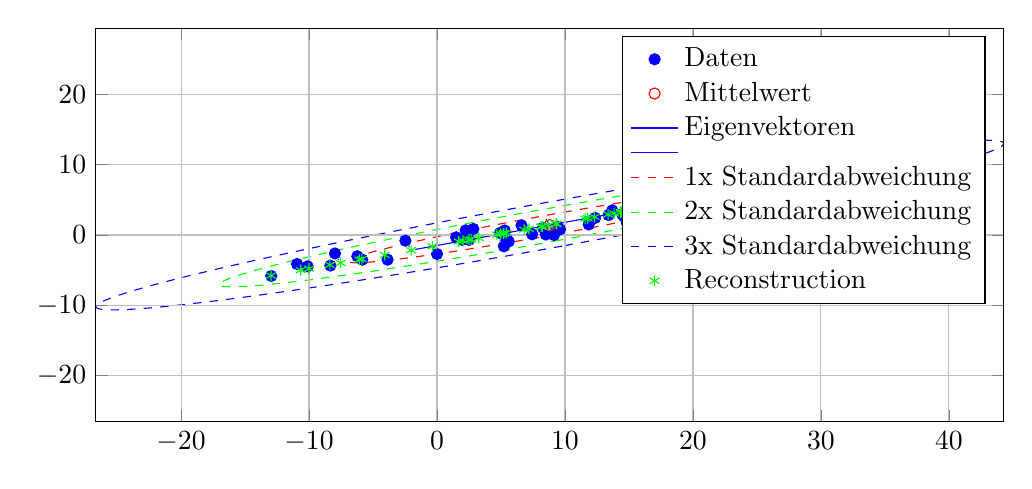
\begin{tikzpicture}

\begin{axis}[%
width=0.95092\figurewidth,
height=\figureheight,
at={(0\figurewidth,0\figureheight)},
scale only axis,
separate axis lines,
every outer x axis line/.append style={black},
every x tick label/.append style={font=\color{black}},
xmin=-26.656869505919,
xmax=44.2809467595858,
xmajorgrids,
every outer y axis line/.append style={black},
every y tick label/.append style={font=\color{black}},
ymin=-26.5653116066968,
ymax=29.3840305769029,
ymajorgrids,
every outer z axis line/.append style={black},
every z tick label/.append style={font=\color{black}},
zmin=-0.199366777294997,
zmax=1.199366777295,
zmajorgrids,
view={0}{90},
legend style={legend cell align=left,align=left,draw=black}
]
\addplot [color=blue,only marks,mark=*,mark options={solid}]
  table[row sep=crcr]{%
5.44472978269709	-0.577289933813434\\
5.22805993100385	-1.61349419707251\\
7.43870466825692	0.100336381683103\\
17.9867387828379	5.75031853523774\\
8.29352813628289	1.01157140895627\\
30.3730913354772	10.7926493491835\\
6.60318793578978	1.37177345507569\\
2.84143991718599	0.856429263381885\\
15.4451966610762	3.48756508581657\\
12.3531091903292	2.42635440824064\\
14.6252626849383	2.60421079873865\\
-10.9387635929438	-4.12081253325755\\
8.49997477137822	0.0670570937670636\\
-8.33525474571426	-4.35064291141613\\
11.8533876174123	1.48679170628117\\
17.6498906665636	4.46330552161421\\
21.7957902617132	7.0546388980878\\
17.5296775004699	6.41643212919879\\
14.8407754035302	1.6965304618198\\
17.7543759736931	4.67306011027556\\
9.43338702977036	1.17591462388934\\
9.61498587566128	0.803017651447581\\
20.2044747193525	5.16472265010514\\
20.8728389278498	4.78998728434885\\
5.29169777657604	0.638628144502255\\
-7.97279740485603	-2.62333345417865\\
-12.953226877787	-5.82144860077072\\
-6.22578573194761	-3.02044631926593\\
-0.000719054247699802	-2.70057294974776\\
14.4711755856635	2.95810012862123\\
2.24159088802308	0.66132907044002\\
9.14665607150171	-0.00170154930304056\\
13.6939096941233	3.49902389303887\\
-3.86210853860879	-3.51063256772806\\
1.49750180459497	-0.33175520459092\\
2.50618354370613	-0.698436589563464\\
1.98210580859646	-0.683896919629093\\
5.60750581178614	-0.921637027767139\\
17.8717947302458	3.45046983270511\\
4.92528953683873	0.284565540228405\\
16.9431050270731	4.15461037217091\\
13.4032700587016	2.82966763240154\\
11.9185584382323	1.93433790779544\\
19.7503240575992	6.25365189610861\\
31.401608574977	8.22601915643582\\
24.6733281566119	5.62610157558818\\
-5.84033827180256	-3.51074860674999\\
15.2991185966086	3.51413691363539\\
-2.46844330524427	-0.811528812240311\\
-10.1079630699076	-4.45695644857533\\
};
\addlegendentry{Daten};

\addplot [color=red,only marks,mark=o,mark options={solid}]
  table[row sep=crcr]{%
8.81203862683339	1.40935948510302\\
};
\addlegendentry{Mittelwert};

\addplot [color=blue,solid]
  table[row sep=crcr]{%
19.3195667747376	4.86956046177552\\
-1.69548952107083	-2.05084149156947\\
};
\addlegendentry{Eigenvektoren};

\addplot [color=blue,solid]
  table[row sep=crcr]{%
8.52125195291776	2.29238598610764\\
9.10282530074901	0.526332984098401\\
};
\addlegendentry{};

\addplot3 [color=red,dashed]
 table[row sep=crcr] {%
9.24838850837491	0.0843038904880058	1\\
8.75290623626761	-0.0781370761031068	1\\
8.25748232069066	-0.239110063175945	1\\
7.76260568523548	-0.398456209826773	1\\
7.26876471339409	-0.556018260646939	1\\
6.77644676658354	-0.71164072091498	1\\
6.28613770317907	-0.86517001005114	1\\
5.79832139903053	-1.01645461318286	1\\
5.31347926993535	-1.16534523067165	1\\
4.83208979653924	-1.31169492545384	1\\
4.35462805213358	-1.45535926804969	1\\
3.88156523381544	-1.59619647909787	1\\
3.41336819747295	-1.73406756927455	1\\
2.95049899705486	-1.86883647645911	1\\
2.49341442857911	-2.00037020001099	1\\
2.04256557933029	-2.12853893202533	1\\
1.59839738269096	-2.25321618543761	1\\
1.16134817904615	-2.37427891885119	1\\
0.731849283194247	-2.49160765796427	1\\
0.310324558691436	-2.6050866134766	1\\
-0.102810000450498	-2.7146037953596	1\\
-0.50714668030002	-2.82005112337689	1\\
-0.902286449370278	-2.92132453374655	1\\
-1.287839352415	-3.01832408183942	1\\
-1.66342489526726	-3.11095404081243	1\\
-2.02867242034123	-3.19912299607943	1\\
-2.38322147242656	-3.28274393552634	1\\
-2.72672215441404	-3.3617343353816	1\\
-3.0588354726019	-3.43601624165717	1\\
-3.37923367124163	-3.50551634707974	1\\
-3.68760055599329	-3.57016606343609	1\\
-3.98363180597122	-3.62990158926143	1\\
-4.267035274072	-3.68466397280374	1\\
-4.53753127528831	-3.73439917020201	1\\
-4.79485286272433	-3.77905809882099	1\\
-5.03874609104008	-3.81859668568989	1\\
-5.26897026706478	-3.85297591099701	1\\
-5.48529818733202	-3.88216184659764	1\\
-5.68751636230207	-3.90612568949699	1\\
-5.87542522705033	-3.92484379027531	1\\
-6.0488393382138	-3.93829767642699	1\\
-6.20758755700132	-3.94647407059073	1\\
-6.35151321808683	-3.94936490365261	1\\
-6.48047428421921	-3.94696732270942	1\\
-6.59434348639584	-3.9392836938841	1\\
-6.69300844946176	-3.92632159999064	1\\
-6.77637180301041	-3.90809383305077	1\\
-6.84435127747639	-3.8846183816698	1\\
-6.89687978532568	-3.85591841328402	1\\
-6.93390548726287	-3.82202225129724	1\\
-6.95539184339032	-3.782963347129	1\\
-6.96131764926862	-3.73878024720209	1\\
-6.95167705684277	-3.68951655490182	1\\
-6.9264795802136	-3.63522088754484	1\\
-6.88575008624841	-3.57594682839963	1\\
-6.8295287700404	-3.51175287380631	1\\
-6.75787111524099	-3.44270237544784	1\\
-6.67084783930414	-3.36886347782954	1\\
-6.56854482369675	-3.29030905102867	1\\
-6.45106302914403	-3.2071166187805	1\\
-6.31851839599346	-3.11936828197171	1\\
-6.17104172979564	-3.02715063761675	1\\
-6.00877857221504	-2.93055469339702	1\\
-5.83188905739793	-2.8296757778473	1\\
-5.64054775393929	-2.72461344627798	1\\
-5.43494349260473	-2.61547138252598	1\\
-5.21527917997729	-2.50235729663136	1\\
-4.98177159821312	-2.38538281854045	1\\
-4.73465119110372	-2.26466338794064	1\\
-4.4741618366557	-2.14031814033529	1\\
-4.20056060641264	-2.01246978947141	1\\
-3.91411751175651	-1.88124450623597	1\\
-3.61511523743904	-1.74677179414052	1\\
-3.303848862606	-1.6091843615168	1\\
-2.98062556958971	-1.46861799054969	1\\
-2.64576434075715	-1.32521140327653	1\\
-2.29959564371289	-1.17910612468529	1\\
-1.94246110516748	-1.03044634304643	1\\
-1.57471317379306	-0.879378767616515	1\\
-1.19671477239917	-0.726052483853882	1\\
-0.808838939771674	-0.570618806289301	1\\
-0.411468462528562	-0.413231129196789	1\\
-0.00499549735576288	-0.254044775211997	1\\
0.410178816004189	-0.0932168420475015	1\\
0.833644750628594	0.0690939525436509	1\\
1.26498439676565	0.232727427403223	1\\
1.70377207426088	0.397522096047232	1\\
2.14957475265208	0.563315326033631	1\\
2.60195247851809	0.729943499460884	1\\
3.0604588096597	0.897242174439078	1\\
3.52464125568421	1.06504624737423	1\\
3.99404172455882	1.23319011590557	1\\
4.46819697469217	1.40150784233513	1\\
4.94663907209782	1.56983331738816	1\\
5.42889585218865	1.73800042414296	1\\
5.91449138574628	1.90584320196824	1\\
6.40294644860574	2.07319601030617	1\\
6.89377899459188	2.23989369213968	1\\
7.38650463124077	2.40577173698246	1\\
7.88063709783649	2.57066644323094	1\\
8.37568874529186	2.73441507971804	1\\
8.87117101739915	2.89685604630915	1\\
9.3665949329761	3.05782903338198	1\\
9.86147156843128	3.21717518003281	1\\
10.3553125402727	3.37473723085298	1\\
10.8476304870832	3.53035969112102	1\\
11.3379395504877	3.68388898025718	1\\
11.8257558546362	3.8351735833889	1\\
12.3105979837314	3.98406420087769	1\\
12.7919874571275	4.13041389565988	1\\
13.2694492015332	4.27407823825573	1\\
13.7425120198513	4.41491544930391	1\\
14.2107090561938	4.55278653948059	1\\
14.6735782566119	4.68755544666515	1\\
15.1306628250877	4.81908917021704	1\\
15.5815116743365	4.94725790223137	1\\
16.0256798709758	5.07193515564365	1\\
16.4627290746206	5.19299788905723	1\\
16.8922279704725	5.31032662817031	1\\
17.3137526949753	5.42380558368265	1\\
17.7268872541173	5.53332276556564	1\\
18.1312239339668	5.63877009358293	1\\
18.526363703037	5.74004350395259	1\\
18.9119166060818	5.83704305204546	1\\
19.287502148934	5.92967301101847	1\\
19.652749674008	6.01784196628548	1\\
20.0072987260933	6.10146290573238	1\\
20.3507994080808	6.18045330558764	1\\
20.6829127262687	6.25473521186321	1\\
21.0033109249084	6.32423531728578	1\\
21.3116778096601	6.38888503364213	1\\
21.607709059638	6.44862055946747	1\\
21.8911125277388	6.50338294300979	1\\
22.1616085289551	6.55311814040805	1\\
22.4189301163911	6.59777706902703	1\\
22.6628233447069	6.63731565589593	1\\
22.8930475207316	6.67169488120306	1\\
23.1093754409988	6.70088081680368	1\\
23.3115936159688	6.72484465970303	1\\
23.4995024807171	6.74356276048135	1\\
23.6729165918806	6.75701664663304	1\\
23.8316648106681	6.76519304079677	1\\
23.9755904717536	6.76808387385865	1\\
24.104551537886	6.76568629291547	1\\
24.2184207400626	6.75800266409014	1\\
24.3170857031285	6.74504057019668	1\\
24.4004490566772	6.72681280325681	1\\
24.4684285311432	6.70333735187584	1\\
24.5209570389924	6.67463738349006	1\\
24.5579827409296	6.64074122150328	1\\
24.5794690970571	6.60168231733505	1\\
24.5853949029354	6.55749921740813	1\\
24.5757543105095	6.50823552510787	1\\
24.5505568338804	6.45393985775089	1\\
24.5098273399152	6.39466579860567	1\\
24.4536060237072	6.33047184401235	1\\
24.3819483689078	6.26142134565388	1\\
24.2949250929709	6.18758244803558	1\\
24.1926220773635	6.10902802123471	1\\
24.0751402828108	6.02583558898654	1\\
23.9425956496602	5.93808725217776	1\\
23.7951189834624	5.84586960782279	1\\
23.6328558258818	5.74927366360307	1\\
23.4559663110647	5.64839474805335	1\\
23.2646250076061	5.54333241648402	1\\
23.0590207462715	5.43419035273203	1\\
22.8393564336441	5.3210762668374	1\\
22.6058488518799	5.2041017887465	1\\
22.3587284447705	5.08338235814668	1\\
22.0982390903225	4.95903711054133	1\\
21.8246378600794	4.83118875967745	1\\
21.5381947654233	4.69996347644202	1\\
21.2391924911058	4.56549076434657	1\\
20.9279261162728	4.42790333172285	1\\
20.6047028232565	4.28733696075573	1\\
20.2698415944239	4.14393037348258	1\\
19.9236728973797	3.99782509489134	1\\
19.5665383588343	3.84916531325248	1\\
19.1987904274598	3.69809773782256	1\\
18.8207920260659	3.54477145405992	1\\
18.4329161934385	3.38933777649534	1\\
18.0355457161953	3.23195009940283	1\\
17.6290727510225	3.07276374541804	1\\
17.2138984376626	2.91193581225355	1\\
16.7904325030382	2.74962501766239	1\\
16.3590928569011	2.58599154280282	1\\
15.9203051794059	2.42119687415881	1\\
15.4745025010147	2.25540364417241	1\\
15.0221247751487	2.08877547074516	1\\
14.5636184440071	1.92147679576696	1\\
14.0994359979826	1.75367272283182	1\\
13.630035529108	1.58552885430047	1\\
13.1558802789746	1.41721112787092	1\\
12.677438181569	1.24888565281788	1\\
12.1951814014781	1.08071854606308	1\\
11.7095858679205	0.912875768237808	1\\
11.221130805061	0.745522959899876	1\\
10.7302982590749	0.578825278066364	1\\
10.237572622426	0.412947233223584	1\\
9.74344015583029	0.248052526975103	1\\
9.24838850837491	0.0843038904880071	1\\
};
 \addlegendentry{1x Standardabweichung};

\addplot3 [color=green,dashed]
 table[row sep=crcr] {%
9.52639580242302	-0.759915704624156	1\\
8.71523179979542	-1.02585108126304	1\\
7.90416333381847	-1.28938319907945	1\\
7.09399083114662	-1.55025198368973	1\\
6.28551383422669	-1.80819998909853	1\\
5.47953021224603	-2.06297265176696	1\\
4.67683537373195	-2.31431854183604	1\\
3.87822148157954	-2.56198961125762	1\\
3.08447667128253	-2.80574143858789	1\\
2.29638427313872	-3.04533347020177	1\\
1.51472203919752	-3.28052925769037	1\\
0.740261375712608	-3.51109669120695	1\\
-0.026233418142926	-3.7368082285314	1\\
-0.784005904547584	-3.95744111962684	1\\
-1.53230825354426	-4.1727776264671	1\\
-2.27040198105814	-4.38260523791783	1\\
-2.99755867769131	-4.58671687945931	1\\
-3.71306072757486	-4.78491111754404	1\\
-4.41620201656919	-4.97699235838731	1\\
-5.10628862911333	-5.16277104099465	1\\
-5.78263953303586	-5.34206382423567	1\\
-6.44458725165144	-5.51469376777959	1\\
-7.09147852247973	-5.68049050671399	1\\
-7.72267494193654	-5.83929041967444	1\\
-8.33755359536113	-5.99093679031897	1\\
-8.93550767175778	-6.13527996198826	1\\
-9.51594706264495	-6.27217748539864	1\\
-10.0782989444211	-6.40149425922232	1\\
-10.6220083436726	-6.52310266341615	1\\
-11.1465386848651	-6.63688268516716	1\\
-11.6513723198792	-6.7427220373307	1\\
-12.1360110388664	-6.84051626924433	1\\
-12.5999765619222	-6.93016886980799	1\\
-13.0428110110907	-7.01159136272881	1\\
-13.4640773622345	-7.08470339383654	1\\
-13.8633598763252	-7.14943281038339	1\\
-14.2402645097273	-7.20571573225012	1\\
-14.5944193030719	-7.25349661498795	1\\
-14.9254747483356	-7.29272830463428	1\\
-15.2331041337628	-7.32337208424794	1\\
-15.5170038662904	-7.34539771211811	1\\
-15.7768937711583	-7.35878345160926	1\\
-16.0125173684072	-7.3635160926126	1\\
-16.2236421259937	-7.35959096458284	1\\
-16.4100596892715	-7.34701194114746	1\\
-16.5715860866122	-7.32579143628391	1\\
-16.7080619109628	-7.2959503920685	1\\
-16.8193524771617	-7.25751825800912	1\\
-16.9053479548563	-7.21053296198211	1\\
-16.9659634768926	-7.15504087280206	1\\
-17.0011392230683	-7.09109675446135	1\\
-17.0108404791689	-7.0187637120847	1\\
-16.9950576712259	-6.93811312965207	1\\
-16.9538063749652	-6.84922459955127	1\\
-16.8871273004358	-6.75218584402984	1\\
-16.7950862518342	-6.64709262862388	1\\
-16.6777740625629	-6.53404866764891	1\\
-16.5353065055897	-6.41316552184647	1\\
-16.3678241791927	-6.28456248828706	1\\
-16.1754923682079	-6.14836648263837	1\\
-15.9585008809122	-6.00471191391483	1\\
-15.7170638617058	-5.85374055183215	1\\
-15.4514195797777	-5.69560138689771	1\\
-15.1618301939624	-5.53045048337493	1\\
-14.8485814940213	-5.35845082526666	1\\
-14.5119826186021	-5.17977215546971	1\\
-14.152365750157	-4.99459080825901	1\\
-13.7700857871179	-4.80308953526706	1\\
-13.3655199936551	-4.60545732513005	1\\
-12.939067627363	-4.40188921697898	1\\
-12.4911495452409	-4.19258610795952	1\\
-12.0222077883581	-3.97775455497079	1\\
-11.5327051456125	-3.75760657081867	1\\
-11.0231246970142	-3.53235941498472	1\\
-10.4939693369435	-3.30223537921734	1\\
-9.94576127785517	-3.06746156815662	1\\
-9.37904153491755	-2.82826967520949	1\\
-8.794369392096	-2.5848957538963	1\\
-8.19232185020716	-2.33757998489449	1\\
-7.57349305748882	-2.08656643900928	1\\
-6.93849372324726	-1.83210283630523	1\\
-6.28795051516097	-1.57444030163643	1\\
-5.62250544083533	-1.31383311681663	1\\
-4.94281521421852	-1.05053846967377	1\\
-4.24955060750422	-0.784816200236618	1\\
-3.5433957891604	-0.516928544304078	1\\
-2.82504764873769	-0.247139874650089	1\\
-2.09521510912344	0.0242835598803852	1\\
-1.35461842692049	0.297073897126815	1\\
-0.60398848164087	0.570961925960707	1\\
0.15593394558409	0.845677351964512	1\\
0.924398903065249	1.12094906417955	1\\
1.70064800866748	1.39650540265983	1\\
2.48391519824126	1.6720744265676	1\\
3.27342748163545	1.94738418254609	1\\
4.06840570554534	2.22216297310472	1\\
4.86806532244278	2.49613962475164	1\\
5.67161716482999	2.76904375560928	1\\
6.47826822405252	3.04060604224862	1\\
7.28722243290308	3.31055848547882	1\\
8.09768145124375	3.5786346748302	1\\
8.90884545387135	3.84457005146908	1\\
9.71991391984829	4.10810216928549	1\\
10.5300864225201	4.36897095389577	1\\
11.3385634194401	4.62691895930457	1\\
12.1445470414207	4.881691621973	1\\
12.9472418799348	5.13303751204208	1\\
13.7458557720872	5.38070858146366	1\\
14.5396005823842	5.62446040879393	1\\
15.327692980528	5.86405244040781	1\\
16.1093552144692	6.0992482278964	1\\
16.8838158779542	6.32981566141299	1\\
17.6503106718097	6.55552719873744	1\\
18.4080831582144	6.77616008983288	1\\
19.156385507211	6.99149659667314	1\\
19.8944792347249	7.20132420812387	1\\
20.6216359313581	7.40543584966535	1\\
21.3371379812416	7.60363008775008	1\\
22.040279270236	7.79571132859335	1\\
22.7303658827801	7.98149001120069	1\\
23.4067167867026	8.16078279444172	1\\
24.0686645053182	8.33341273798563	1\\
24.7155557761465	8.49920947692003	1\\
25.3467521956033	8.65800938988048	1\\
25.9616308490279	8.80965576052501	1\\
26.5595849254246	8.95399893219431	1\\
27.1400243163117	9.09089645560468	1\\
27.7023761980879	9.22021322942836	1\\
28.2460855973394	9.3418216336222	1\\
28.7706159385318	9.4556016553732	1\\
29.2754495735459	9.56144100753674	1\\
29.7600882925331	9.65923523945037	1\\
30.224053815589	9.74888784001403	1\\
30.6668882647575	9.83031033293485	1\\
31.0881546159013	9.90342236404258	1\\
31.487437129992	9.96815178058943	1\\
31.8643417633941	10.0244347024562	1\\
32.2184965567387	10.072215585194	1\\
32.5495520020024	10.1114472748403	1\\
32.8571813874295	10.142091054454	1\\
33.1410811199572	10.1641166823241	1\\
33.4009710248251	10.1775024218153	1\\
33.6365946220739	10.1822350628186	1\\
33.8477193796604	10.1783099347889	1\\
34.0341369429383	10.1657309113535	1\\
34.1956633402789	10.14451040649	1\\
34.3321391646296	10.1146693622745	1\\
34.4434297308285	10.0762372282152	1\\
34.5294252085231	10.0292519321882	1\\
34.5900407305593	9.97375984300811	1\\
34.6252164767351	9.90981572466739	1\\
34.6349177328357	9.83748268229074	1\\
34.6191349248927	9.75683209985812	1\\
34.5778836286319	9.66794356975731	1\\
34.5112045541026	9.57090481423589	1\\
34.419163505501	9.46581159882992	1\\
34.3018513162297	9.35276763785495	1\\
34.1593837592564	9.23188449205252	1\\
33.9919014328595	9.1032814584931	1\\
33.7995696218747	8.96708545284441	1\\
33.582578134579	8.82343088412087	1\\
33.3411411153726	8.67245952203819	1\\
33.0754968334445	8.51432035710376	1\\
32.7859074476292	8.34916945358097	1\\
32.4726587476881	8.17716979547271	1\\
32.1360598722689	7.99849112567575	1\\
31.7764430038238	7.81330977846506	1\\
31.3941630407846	7.6218085054731	1\\
30.9895972473219	7.4241762953361	1\\
30.5631448810298	7.22060818718503	1\\
30.1152267989077	7.01130507816556	1\\
29.6462850420249	6.79647352517684	1\\
29.1567823992793	6.57632554102471	1\\
28.647201950681	6.35107838519077	1\\
28.1180465906103	6.12095434942339	1\\
27.569838531522	5.88618053836267	1\\
27.0031187885843	5.64698864541553	1\\
26.4184466457628	5.40361472410234	1\\
25.8163991038739	5.15629895510053	1\\
25.1975703111556	4.90528540921532	1\\
24.562570976914	4.65082180651127	1\\
23.9120277688278	4.39315927184247	1\\
23.2465826945021	4.13255208702268	1\\
22.5668924678853	3.86925743987982	1\\
21.873627861171	3.60353517044266	1\\
21.1674730428272	3.33564751451012	1\\
20.4491249024045	3.06585884485614	1\\
19.7192923627902	2.79443541032566	1\\
18.9786956805873	2.52164507307923	1\\
18.2280657353076	2.24775704424534	1\\
17.4681433080827	1.97304161824153	1\\
16.6996783506015	1.69776990602649	1\\
15.9234292449993	1.42221356754621	1\\
15.1401620554255	1.14664454363845	1\\
14.3506497720313	0.871334787659955	1\\
13.5556715481215	0.59655599710133	1\\
12.756011931224	0.322579345454407	1\\
11.9524600888368	0.0496752145967623	1\\
11.1458090296143	-0.221887072042572	1\\
10.3368548207637	-0.49183951527278	1\\
9.52639580242302	-0.759915704624154	1\\
};
 \addlegendentry{2x Standardabweichung};

\addplot3 [color=blue,dashed]
 table[row sep=crcr] {%
9.7932409525288	-1.57023942419164	1\\
8.67907001242219	-1.93551385406963	1\\
7.5650302962845	-2.29748729779332	1\\
6.45222122681593	-2.65580253127532	1\\
5.34174101221696	-3.01010594064011	1\\
4.23468556238952	-3.36004787119823	1\\
3.13214740740614	-3.7052829725132	1\\
2.03521461931477	-4.04547053922077	1\\
0.944969738342936	-4.38027484726395	1\\
-0.137511295438694	-4.7093654852121	1\\
-1.2111602039393	-5.03241768033717	1\\
-2.27491742530939	-5.34911261912513	1\\
-3.32773315960044	-5.65913776190644	1\\
-4.36856840479069	-5.96218715129497	1\\
-5.3963959821547	-6.25796171413099	1\\
-6.41020154996474	-6.54616955663027	1\\
-7.40898460452361	-6.82652625244802	1\\
-8.39175946754099	-7.09875512337334	1\\
-9.35755625887895	-7.36258751237722	1\\
-10.3054218537065	-7.61776304874459	1\\
-11.2344208231187	-7.86402990502875	1\\
-12.1436363572922	-8.10114504557473	1\\
-13.0321711702656	-8.32887446636605	1\\
-13.8991483854528	-8.54699342595851	1\\
-14.7437124010136	-8.7552866672728	1\\
-15.5650297342302	-8.9535486300273	1\\
-16.3622898440536	-9.14158365360123	1\\
-17.1347059310098	-9.31920617012806	1\\
-17.8815157136758	-9.4862408876286	1\\
-18.6019821809596	-9.64252296300303	1\\
-19.2953943194409	-9.78789816471112	1\\
-19.9610678150557	-9.92222302498014	1\\
-20.5983457284317	-10.0453649813902	1\\
-21.2065991432077	-10.1572025076976	1\\
-21.7852277866988	-10.2576252337659	1\\
-22.3336606222924	-10.3465340544889	1\\
-22.8513564129931	-10.4238412275946	1\\
-23.3378042555574	-10.4894704602364	1\\
-23.7925240846943	-10.5433569842854	1\\
-24.2150671468316	-10.585447620248	1\\
-24.605016442981	-10.6157008297482	1\\
-24.9619871402665	-10.6340867565208	1\\
-25.2856269517074	-10.6405872558758	1\\
-25.5756164838833	-10.6351959126052	1\\
-25.8316695521369	-10.6179180473138	1\\
-26.0535334630034	-10.5887707111687	1\\
-26.2409892635888	-10.5477826690717	1\\
-26.3938519576496	-10.4949943712719	1\\
-26.5119706881623	-10.4304579134458	1\\
-26.5952288862004	-10.3542369852858	1\\
-26.6435443859743	-10.2664068076458	1\\
-26.656869505919	-10.1670540583072	1\\
-26.6351910957498	-10.0562767864386	1\\
-26.5785305494404	-9.93418431583304	1\\
-26.4869437841092	-9.80089713701858	1\\
-26.3605211848362	-9.65654678834877	1\\
-26.1993875154636	-9.50127572619012	1\\
-26.0037017954694	-9.33523718433487	1\\
-25.7736571430335	-9.15859502277777	1\\
-25.5094805844545	-8.971523566006	1\\
-25.2114328301012	-8.77420743096198	1\\
-24.8798080171234	-8.56684134484873	1\\
-24.5149334191739	-8.34962995295766	1\\
-24.1171691234291	-8.12278761670828	1\\
-23.6869076752263	-7.88653820209949	1\\
-23.2245736906686	-7.64111485878075	1\\
-22.7306234375806	-7.38675978996161	1\\
-22.2055443852268	-7.12372401338633	1\\
-21.6498547232383	-6.8522671136097	1\\
-21.0641028502222	-6.57265698581841	1\\
-20.4488668325586	-6.28516957145084	1\\
-19.8047538339184	-5.99008858587621	1\\
-19.1323995160667	-5.68770523840171	1\\
-18.4324674115409	-5.37831794488412	1\\
-17.7056482688242	-5.06223203322936	1\\
-16.9526593706607	-4.73975944207072	1\\
-16.1742438261834	-4.41121841292308	1\\
-15.3711698375553	-4.07693317611698	1\\
-14.5442299418471	-3.73723363082239	1\\
-13.694240228898	-3.3924550194781	1\\
-12.8220395359343	-3.04293759694788	1\\
-11.9284886197379	-2.68902629473002	1\\
-11.0144693071833	-2.33107038055157	1\\
-10.0808836249811	-1.96942311368329	1\\
-9.12865290948654	-1.60444139631538	1\\
-8.15871689745156	-1.2364854213381	1\\
-7.17203279861827	-0.865918316874888	1\\
-6.16957435106839	-0.493105787918743	1\\
-5.15233086026136	-0.118415755425536	1\\
-4.12130622270934	0.257782006779527	1\\
-3.07751793525246	0.635116236924066	1\\
-2.02199609091237	1.01321455167903	1\\
-0.95578236231473	1.39170381365613	1\\
0.120071026315898	1.77021049964936	1\\
1.20450233757425	2.1483610692573	1\\
2.29644136868114	2.52578233352242	1\\
3.39481050764421	2.90210182322351	1\\
4.49852579673105	3.27694815645785	1\\
5.60649800220449	3.64995140515027	1\\
6.71763368926483	4.02074346012754	1\\
7.83083630113797	4.38895839439768	1\\
8.94500724124457	4.75423282427567	1\\
10.0590469573823	5.11620626799935	1\\
11.1718560268508	5.47452150148136	1\\
12.2823362414498	5.82882491084615	1\\
13.3893916912772	6.17876684140426	1\\
14.4919298462606	6.52400194271924	1\\
15.588862634352	6.86418950942681	1\\
16.6791075153238	7.19899381746999	1\\
17.7615885491055	7.52808445541814	1\\
18.8352374576061	7.8511366505432	1\\
19.8989946789762	8.16783158933117	1\\
20.9518104132672	8.47785673211248	1\\
21.9926456584575	8.78090612150101	1\\
23.0204732358215	9.07668068433703	1\\
24.0342788036315	9.3648885268363	1\\
25.0330618581904	9.64524522265406	1\\
26.0158367212077	9.91747409357938	1\\
26.9816335125457	10.1813064825833	1\\
27.9294991073732	10.4364820189506	1\\
28.8584980767855	10.6827488752348	1\\
29.7677136109589	10.9198640157808	1\\
30.6562484239324	11.1475934365721	1\\
31.5232256391195	11.3657123961645	1\\
32.3677896546804	11.5740056374788	1\\
33.189106987897	11.7722676002333	1\\
33.9863670977204	11.9603026238073	1\\
34.7587831846765	12.1379251403341	1\\
35.5055929673426	12.3049598578346	1\\
36.2260594346263	12.4612419332091	1\\
36.9194715731077	12.6066171349172	1\\
37.5851450687225	12.7409419951862	1\\
38.2224229820985	12.8640839515963	1\\
38.8306763968745	12.9759214779036	1\\
39.4093050403656	13.076344203972	1\\
39.9577378759592	13.165253024695	1\\
40.4754336666598	13.2425601978006	1\\
40.9618815092241	13.3081894304425	1\\
41.4166013383611	13.3620759544914	1\\
41.8391444004983	13.404166590454	1\\
42.2290936966478	13.4344197999542	1\\
42.5860643939332	13.4528057267268	1\\
42.9097042053741	13.4593062260818	1\\
43.1996937375501	13.4539148828112	1\\
43.4557468058036	13.4366370175198	1\\
43.6776107166702	13.4074896813747	1\\
43.8650665172555	13.3665016392778	1\\
44.0179292113164	13.3137133414779	1\\
44.136047941829	13.2491768836518	1\\
44.2193061398671	13.1729559554919	1\\
44.2676216396411	13.0851257778519	1\\
44.2809467595858	12.9857730285133	1\\
44.2592683494166	12.8749957566447	1\\
44.2026078031072	12.7529032860391	1\\
44.111021037776	12.6196161072246	1\\
43.9845984385029	12.4752657585548	1\\
43.8234647691304	12.3199946963962	1\\
43.6277790491361	12.1539561545409	1\\
43.3977343967003	11.9773139929838	1\\
43.1335578381213	11.790242536212	1\\
42.835510083768	11.592926401168	1\\
42.5038852707902	11.3855603150548	1\\
42.1390106728407	11.1683489231637	1\\
41.7412463770959	10.9415065869143	1\\
41.310984928893	10.7052571723055	1\\
40.8486509443354	10.4598338289868	1\\
40.3547006912474	10.2054787601677	1\\
39.8296216388936	9.94244298359238	1\\
39.2739319769051	9.67098608381574	1\\
38.688180103889	9.39137595602445	1\\
38.0729440862253	9.10388854165688	1\\
37.4288310875852	8.80880755608225	1\\
36.7564767697335	8.50642420860776	1\\
36.0565446652077	8.19703691509017	1\\
35.329725522491	7.8809510034354	1\\
34.5767366243275	7.55847841227676	1\\
33.7983210798501	7.22993738312913	1\\
32.9952470912221	6.89565214632302	1\\
32.1683071955138	6.55595260102843	1\\
31.3183174825648	6.21117398968414	1\\
30.4461167896011	5.86165656715393	1\\
29.5525658734047	5.50774526493607	1\\
28.6385465608501	5.14978935075762	1\\
27.7049608786479	4.78814208388935	1\\
26.7527301631533	4.42316036652143	1\\
25.7827941511184	4.05520439154415	1\\
24.7961100522851	3.68463728708094	1\\
23.7936516047352	3.31182475812479	1\\
22.7764081139281	2.93713472563158	1\\
21.7453834763761	2.56093696342652	1\\
20.7015951889192	2.18360273328198	1\\
19.6460733445792	1.80550441852701	1\\
18.5798596159815	1.42701515654992	1\\
17.5040062273509	1.04850847055668	1\\
16.4195749160925	0.670357900948747	1\\
15.3276358849857	0.292936636683629	1\\
14.2292667460226	-0.0833828530174632	1\\
13.1255514569357	-0.458229186251797	1\\
12.0175792514623	-0.831232434944227	1\\
10.906443564402	-1.2020244899215	1\\
9.79324095252881	-1.57023942419163	1\\
};
 \addlegendentry{3x Standardabweichung};

\addplot [color=green,only marks,mark=asterisk,mark options={solid}]
  table[row sep=crcr]{%
5.18395301325052	0.214606046724195\\
4.68063528597355	0.0488600723155777\\
7.18416580834757	0.873289817990426\\
18.3787982133788	4.55975893195656\\
8.22607721249022	1.21639837858369\\
31.0513728222213	8.73292453486934\\
6.80812139555047	0.749455817632094\\
3.26129545216773	-0.418538254868026\\
15.4136639415787	3.58331991044472\\
12.3088119885049	2.56087089967594\\
14.4115117407117	3.25330432776876\\
-10.6494273501499	-4.99943453696843\\
8.13172107772593	1.18532625723691\\
-8.36890942620353	-4.24844436718885\\
11.5788457161899	2.32048800725363\\
17.6925470347527	4.33377171925532\\
22.2026963349608	5.8189947701811\\
18.1643482920514	4.48913910426925\\
14.336277712165	3.22852924695127\\
17.8491260645934	4.38533426606508\\
9.30324422904611	1.57111685378183\\
9.35629280184757	1.58858611209215\\
20.2055905705696	5.16133416540384\\
20.6972363170477	5.32323647660342\\
5.40712925582602	0.288099511758011\\
-7.52874698767539	-3.97177312258805\\
-12.9720496117722	-5.76428995348327\\
-6.0706298932084	-3.4916051779146\\
-0.359553033760195	-1.61090845754884\\
14.3776363682898	3.2421489356452\\
2.66216959849475	-0.615834501411271\\
8.69470772470587	1.37072161552791\\
13.8371160245066	3.06415188485042\\
-4.08382903443411	-2.83733804912696\\
1.69584247497977	-0.934052640778192\\
2.49690400698656	-0.670257592465379\\
2.02841828232122	-0.824533149877753\\
5.22850214467479	0.229276380783203\\
17.5918385050928	4.30060771076699\\
4.97137975865079	0.144604218242095\\
16.9631986911647	4.09359231499446\\
13.3760519591402	2.91232033067014\\
11.7706019452516	2.38363464666707\\
20.1193806311995	5.13294464198709\\
31.2167474424844	8.7873835298391\\
24.3743107266114	6.53412226098343\\
-5.86855584958259	-3.42506081150682\\
15.2897714368988	3.542521260214\\
-2.02463556803213	-2.15923153888907\\
-9.99977190591748	-4.78549855021764\\
};
\addlegendentry{Reconstruction};

\addplot [color=blue,dotted,forget plot]
  table[row sep=crcr]{%
5.44472978269709	-0.577289933813434\\
5.18395301325052	0.214606046724195\\
};
\addplot [color=blue,dotted,forget plot]
  table[row sep=crcr]{%
5.22805993100385	-1.61349419707251\\
4.68063528597355	0.0488600723155777\\
};
\addplot [color=blue,dotted,forget plot]
  table[row sep=crcr]{%
7.43870466825692	0.100336381683103\\
7.18416580834757	0.873289817990426\\
};
\addplot [color=blue,dotted,forget plot]
  table[row sep=crcr]{%
17.9867387828379	5.75031853523774\\
18.3787982133788	4.55975893195656\\
};
\addplot [color=blue,dotted,forget plot]
  table[row sep=crcr]{%
8.29352813628289	1.01157140895627\\
8.22607721249022	1.21639837858369\\
};
\addplot [color=blue,dotted,forget plot]
  table[row sep=crcr]{%
30.3730913354772	10.7926493491835\\
31.0513728222213	8.73292453486934\\
};
\addplot [color=blue,dotted,forget plot]
  table[row sep=crcr]{%
6.60318793578978	1.37177345507569\\
6.80812139555047	0.749455817632094\\
};
\addplot [color=blue,dotted,forget plot]
  table[row sep=crcr]{%
2.84143991718599	0.856429263381885\\
3.26129545216773	-0.418538254868026\\
};
\addplot [color=blue,dotted,forget plot]
  table[row sep=crcr]{%
15.4451966610762	3.48756508581657\\
15.4136639415787	3.58331991044472\\
};
\addplot [color=blue,dotted,forget plot]
  table[row sep=crcr]{%
12.3531091903292	2.42635440824064\\
12.3088119885049	2.56087089967594\\
};
\addplot [color=blue,dotted,forget plot]
  table[row sep=crcr]{%
14.6252626849383	2.60421079873865\\
14.4115117407117	3.25330432776876\\
};
\addplot [color=blue,dotted,forget plot]
  table[row sep=crcr]{%
-10.9387635929438	-4.12081253325755\\
-10.6494273501499	-4.99943453696843\\
};
\addplot [color=blue,dotted,forget plot]
  table[row sep=crcr]{%
8.49997477137822	0.0670570937670636\\
8.13172107772593	1.18532625723691\\
};
\addplot [color=blue,dotted,forget plot]
  table[row sep=crcr]{%
-8.33525474571426	-4.35064291141613\\
-8.36890942620353	-4.24844436718885\\
};
\addplot [color=blue,dotted,forget plot]
  table[row sep=crcr]{%
11.8533876174123	1.48679170628117\\
11.5788457161899	2.32048800725363\\
};
\addplot [color=blue,dotted,forget plot]
  table[row sep=crcr]{%
17.6498906665636	4.46330552161421\\
17.6925470347527	4.33377171925532\\
};
\addplot [color=blue,dotted,forget plot]
  table[row sep=crcr]{%
21.7957902617132	7.0546388980878\\
22.2026963349608	5.8189947701811\\
};
\addplot [color=blue,dotted,forget plot]
  table[row sep=crcr]{%
17.5296775004699	6.41643212919879\\
18.1643482920514	4.48913910426925\\
};
\addplot [color=blue,dotted,forget plot]
  table[row sep=crcr]{%
14.8407754035302	1.6965304618198\\
14.336277712165	3.22852924695127\\
};
\addplot [color=blue,dotted,forget plot]
  table[row sep=crcr]{%
17.7543759736931	4.67306011027556\\
17.8491260645934	4.38533426606508\\
};
\addplot [color=blue,dotted,forget plot]
  table[row sep=crcr]{%
9.43338702977036	1.17591462388934\\
9.30324422904611	1.57111685378183\\
};
\addplot [color=blue,dotted,forget plot]
  table[row sep=crcr]{%
9.61498587566128	0.803017651447581\\
9.35629280184757	1.58858611209215\\
};
\addplot [color=blue,dotted,forget plot]
  table[row sep=crcr]{%
20.2044747193525	5.16472265010514\\
20.2055905705696	5.16133416540384\\
};
\addplot [color=blue,dotted,forget plot]
  table[row sep=crcr]{%
20.8728389278498	4.78998728434885\\
20.6972363170477	5.32323647660342\\
};
\addplot [color=blue,dotted,forget plot]
  table[row sep=crcr]{%
5.29169777657604	0.638628144502255\\
5.40712925582602	0.288099511758011\\
};
\addplot [color=blue,dotted,forget plot]
  table[row sep=crcr]{%
-7.97279740485603	-2.62333345417865\\
-7.52874698767539	-3.97177312258805\\
};
\addplot [color=blue,dotted,forget plot]
  table[row sep=crcr]{%
-12.953226877787	-5.82144860077072\\
-12.9720496117722	-5.76428995348327\\
};
\addplot [color=blue,dotted,forget plot]
  table[row sep=crcr]{%
-6.22578573194761	-3.02044631926593\\
-6.0706298932084	-3.4916051779146\\
};
\addplot [color=blue,dotted,forget plot]
  table[row sep=crcr]{%
-0.000719054247699802	-2.70057294974776\\
-0.359553033760195	-1.61090845754884\\
};
\addplot [color=blue,dotted,forget plot]
  table[row sep=crcr]{%
14.4711755856635	2.95810012862123\\
14.3776363682898	3.2421489356452\\
};
\addplot [color=blue,dotted,forget plot]
  table[row sep=crcr]{%
2.24159088802308	0.66132907044002\\
2.66216959849475	-0.615834501411271\\
};
\addplot [color=blue,dotted,forget plot]
  table[row sep=crcr]{%
9.14665607150171	-0.00170154930304056\\
8.69470772470587	1.37072161552791\\
};
\addplot [color=blue,dotted,forget plot]
  table[row sep=crcr]{%
13.6939096941233	3.49902389303887\\
13.8371160245066	3.06415188485042\\
};
\addplot [color=blue,dotted,forget plot]
  table[row sep=crcr]{%
-3.86210853860879	-3.51063256772806\\
-4.08382903443411	-2.83733804912696\\
};
\addplot [color=blue,dotted,forget plot]
  table[row sep=crcr]{%
1.49750180459497	-0.33175520459092\\
1.69584247497977	-0.934052640778192\\
};
\addplot [color=blue,dotted,forget plot]
  table[row sep=crcr]{%
2.50618354370613	-0.698436589563464\\
2.49690400698656	-0.670257592465379\\
};
\addplot [color=blue,dotted,forget plot]
  table[row sep=crcr]{%
1.98210580859646	-0.683896919629093\\
2.02841828232122	-0.824533149877753\\
};
\addplot [color=blue,dotted,forget plot]
  table[row sep=crcr]{%
5.60750581178614	-0.921637027767139\\
5.22850214467479	0.229276380783203\\
};
\addplot [color=blue,dotted,forget plot]
  table[row sep=crcr]{%
17.8717947302458	3.45046983270511\\
17.5918385050928	4.30060771076699\\
};
\addplot [color=blue,dotted,forget plot]
  table[row sep=crcr]{%
4.92528953683873	0.284565540228405\\
4.97137975865079	0.144604218242095\\
};
\addplot [color=blue,dotted,forget plot]
  table[row sep=crcr]{%
16.9431050270731	4.15461037217091\\
16.9631986911647	4.09359231499446\\
};
\addplot [color=blue,dotted,forget plot]
  table[row sep=crcr]{%
13.4032700587016	2.82966763240154\\
13.3760519591402	2.91232033067014\\
};
\addplot [color=blue,dotted,forget plot]
  table[row sep=crcr]{%
11.9185584382323	1.93433790779544\\
11.7706019452516	2.38363464666707\\
};
\addplot [color=blue,dotted,forget plot]
  table[row sep=crcr]{%
19.7503240575992	6.25365189610861\\
20.1193806311995	5.13294464198709\\
};
\addplot [color=blue,dotted,forget plot]
  table[row sep=crcr]{%
31.401608574977	8.22601915643582\\
31.2167474424844	8.7873835298391\\
};
\addplot [color=blue,dotted,forget plot]
  table[row sep=crcr]{%
24.6733281566119	5.62610157558818\\
24.3743107266114	6.53412226098343\\
};
\addplot [color=blue,dotted,forget plot]
  table[row sep=crcr]{%
-5.84033827180256	-3.51074860674999\\
-5.86855584958259	-3.42506081150682\\
};
\addplot [color=blue,dotted,forget plot]
  table[row sep=crcr]{%
15.2991185966086	3.51413691363539\\
15.2897714368988	3.542521260214\\
};
\addplot [color=blue,dotted,forget plot]
  table[row sep=crcr]{%
-2.46844330524427	-0.811528812240311\\
-2.02463556803213	-2.15923153888907\\
};
\addplot [color=blue,dotted,forget plot]
  table[row sep=crcr]{%
-10.1079630699076	-4.45695644857533\\
-9.99977190591748	-4.78549855021764\\
};
\end{axis}
\end{tikzpicture}%
				\caption{Hauptvektor}
				\label{fig:projection1}
			\end{subfigure}
			\qquad
			\begin{subfigure}{0.45\textwidth}
				\centering
				% This file was created by matlab2tikz.
% Minimal pgfplots version: 1.3
%
%The latest updates can be retrieved from
%  http://www.mathworks.com/matlabcentral/fileexchange/22022-matlab2tikz
%where you can also make suggestions and rate matlab2tikz.
%
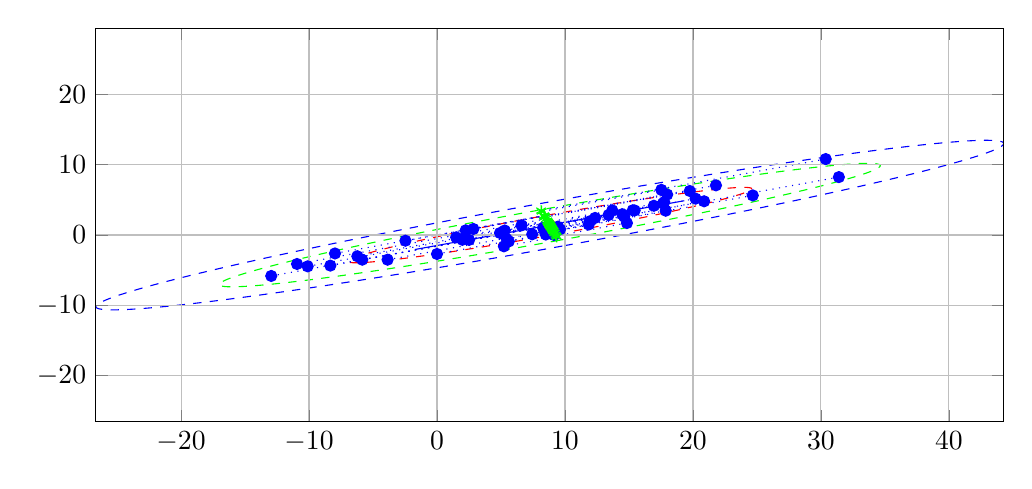
\begin{tikzpicture}

\begin{axis}[%
width=0.95092\figurewidth,
height=\figureheight,
at={(0\figurewidth,0\figureheight)},
scale only axis,
separate axis lines,
every outer x axis line/.append style={black},
every x tick label/.append style={font=\color{black}},
xmin=-26.656869505919,
xmax=44.2809467595858,
xmajorgrids,
every outer y axis line/.append style={black},
every y tick label/.append style={font=\color{black}},
ymin=-26.5653116066968,
ymax=29.3840305769029,
ymajorgrids,
every outer z axis line/.append style={black},
every z tick label/.append style={font=\color{black}},
zmin=-0.199366777294997,
zmax=1.199366777295,
zmajorgrids,
view={0}{90}
]
\addplot [color=blue,only marks,mark=*,mark options={solid},forget plot]
  table[row sep=crcr]{%
5.44472978269709	-0.577289933813434\\
5.22805993100385	-1.61349419707251\\
7.43870466825692	0.100336381683103\\
17.9867387828379	5.75031853523774\\
8.29352813628289	1.01157140895627\\
30.3730913354772	10.7926493491835\\
6.60318793578978	1.37177345507569\\
2.84143991718599	0.856429263381885\\
15.4451966610762	3.48756508581657\\
12.3531091903292	2.42635440824064\\
14.6252626849383	2.60421079873865\\
-10.9387635929438	-4.12081253325755\\
8.49997477137822	0.0670570937670636\\
-8.33525474571426	-4.35064291141613\\
11.8533876174123	1.48679170628117\\
17.6498906665636	4.46330552161421\\
21.7957902617132	7.0546388980878\\
17.5296775004699	6.41643212919879\\
14.8407754035302	1.6965304618198\\
17.7543759736931	4.67306011027556\\
9.43338702977036	1.17591462388934\\
9.61498587566128	0.803017651447581\\
20.2044747193525	5.16472265010514\\
20.8728389278498	4.78998728434885\\
5.29169777657604	0.638628144502255\\
-7.97279740485603	-2.62333345417865\\
-12.953226877787	-5.82144860077072\\
-6.22578573194761	-3.02044631926593\\
-0.000719054247699802	-2.70057294974776\\
14.4711755856635	2.95810012862123\\
2.24159088802308	0.66132907044002\\
9.14665607150171	-0.00170154930304056\\
13.6939096941233	3.49902389303887\\
-3.86210853860879	-3.51063256772806\\
1.49750180459497	-0.33175520459092\\
2.50618354370613	-0.698436589563464\\
1.98210580859646	-0.683896919629093\\
5.60750581178614	-0.921637027767139\\
17.8717947302458	3.45046983270511\\
4.92528953683873	0.284565540228405\\
16.9431050270731	4.15461037217091\\
13.4032700587016	2.82966763240154\\
11.9185584382323	1.93433790779544\\
19.7503240575992	6.25365189610861\\
31.401608574977	8.22601915643582\\
24.6733281566119	5.62610157558818\\
-5.84033827180256	-3.51074860674999\\
15.2991185966086	3.51413691363539\\
-2.46844330524427	-0.811528812240311\\
-10.1079630699076	-4.45695644857533\\
};
\addplot [color=red,only marks,mark=o,mark options={solid},forget plot]
  table[row sep=crcr]{%
8.81203862683339	1.40935948510302\\
};
\addplot [color=blue,solid,forget plot]
  table[row sep=crcr]{%
19.3195667747376	4.86956046177552\\
-1.69548952107083	-2.05084149156947\\
};
\addplot [color=blue,solid,forget plot]
  table[row sep=crcr]{%
8.52125195291776	2.29238598610764\\
9.10282530074901	0.526332984098401\\
};
\addplot3 [color=red,dashed]
 table[row sep=crcr] {%
9.24838850837491	0.0843038904880056	1\\
8.75290623626761	-0.0781370761031071	1\\
8.25748232069066	-0.239110063175946	1\\
7.76260568523548	-0.398456209826773	1\\
7.26876471339409	-0.556018260646939	1\\
6.77644676658354	-0.71164072091498	1\\
6.28613770317907	-0.86517001005114	1\\
5.79832139903053	-1.01645461318286	1\\
5.31347926993535	-1.16534523067165	1\\
4.83208979653924	-1.31169492545384	1\\
4.35462805213358	-1.45535926804969	1\\
3.88156523381544	-1.59619647909787	1\\
3.41336819747295	-1.73406756927455	1\\
2.95049899705486	-1.86883647645911	1\\
2.49341442857911	-2.000370200011	1\\
2.04256557933029	-2.12853893202533	1\\
1.59839738269096	-2.25321618543761	1\\
1.16134817904615	-2.37427891885119	1\\
0.731849283194247	-2.49160765796427	1\\
0.310324558691436	-2.60508661347661	1\\
-0.102810000450498	-2.7146037953596	1\\
-0.50714668030002	-2.82005112337689	1\\
-0.902286449370278	-2.92132453374655	1\\
-1.287839352415	-3.01832408183942	1\\
-1.66342489526726	-3.11095404081243	1\\
-2.02867242034123	-3.19912299607943	1\\
-2.38322147242656	-3.28274393552634	1\\
-2.72672215441404	-3.3617343353816	1\\
-3.0588354726019	-3.43601624165717	1\\
-3.37923367124163	-3.50551634707974	1\\
-3.68760055599329	-3.57016606343609	1\\
-3.98363180597122	-3.62990158926143	1\\
-4.267035274072	-3.68466397280374	1\\
-4.53753127528831	-3.73439917020201	1\\
-4.79485286272433	-3.77905809882099	1\\
-5.03874609104008	-3.81859668568989	1\\
-5.26897026706478	-3.85297591099701	1\\
-5.48529818733202	-3.88216184659764	1\\
-5.68751636230207	-3.90612568949699	1\\
-5.87542522705033	-3.92484379027531	1\\
-6.0488393382138	-3.93829767642699	1\\
-6.20758755700132	-3.94647407059073	1\\
-6.35151321808683	-3.94936490365261	1\\
-6.48047428421921	-3.94696732270942	1\\
-6.59434348639584	-3.9392836938841	1\\
-6.69300844946176	-3.92632159999064	1\\
-6.77637180301041	-3.90809383305077	1\\
-6.84435127747639	-3.8846183816698	1\\
-6.89687978532568	-3.85591841328402	1\\
-6.93390548726287	-3.82202225129724	1\\
-6.95539184339032	-3.782963347129	1\\
-6.96131764926862	-3.73878024720209	1\\
-6.95167705684277	-3.68951655490182	1\\
-6.9264795802136	-3.63522088754484	1\\
-6.88575008624841	-3.57594682839963	1\\
-6.8295287700404	-3.51175287380631	1\\
-6.75787111524099	-3.44270237544784	1\\
-6.67084783930414	-3.36886347782954	1\\
-6.56854482369675	-3.29030905102867	1\\
-6.45106302914403	-3.2071166187805	1\\
-6.31851839599346	-3.11936828197171	1\\
-6.17104172979564	-3.02715063761675	1\\
-6.00877857221504	-2.93055469339702	1\\
-5.83188905739793	-2.8296757778473	1\\
-5.64054775393929	-2.72461344627798	1\\
-5.43494349260473	-2.61547138252598	1\\
-5.21527917997729	-2.50235729663136	1\\
-4.98177159821312	-2.38538281854045	1\\
-4.73465119110372	-2.26466338794064	1\\
-4.4741618366557	-2.14031814033529	1\\
-4.20056060641264	-2.01246978947141	1\\
-3.91411751175651	-1.88124450623597	1\\
-3.61511523743904	-1.74677179414052	1\\
-3.303848862606	-1.6091843615168	1\\
-2.98062556958971	-1.46861799054969	1\\
-2.64576434075715	-1.32521140327653	1\\
-2.29959564371289	-1.17910612468529	1\\
-1.94246110516748	-1.03044634304643	1\\
-1.57471317379306	-0.879378767616515	1\\
-1.19671477239917	-0.726052483853882	1\\
-0.808838939771674	-0.570618806289301	1\\
-0.411468462528562	-0.413231129196789	1\\
-0.00499549735576288	-0.254044775211997	1\\
0.410178816004189	-0.0932168420475017	1\\
0.833644750628594	0.0690939525436507	1\\
1.26498439676565	0.232727427403222	1\\
1.70377207426088	0.397522096047231	1\\
2.14957475265208	0.56331532603363	1\\
2.60195247851809	0.729943499460884	1\\
3.0604588096597	0.897242174439078	1\\
3.52464125568421	1.06504624737423	1\\
3.99404172455882	1.23319011590557	1\\
4.46819697469217	1.40150784233513	1\\
4.94663907209782	1.56983331738816	1\\
5.42889585218865	1.73800042414296	1\\
5.91449138574628	1.90584320196824	1\\
6.40294644860574	2.07319601030617	1\\
6.89377899459188	2.23989369213968	1\\
7.38650463124077	2.40577173698246	1\\
7.88063709783649	2.57066644323094	1\\
8.37568874529186	2.73441507971804	1\\
8.87117101739915	2.89685604630915	1\\
9.3665949329761	3.05782903338198	1\\
9.86147156843128	3.21717518003281	1\\
10.3553125402727	3.37473723085298	1\\
10.8476304870832	3.53035969112102	1\\
11.3379395504877	3.68388898025718	1\\
11.8257558546362	3.8351735833889	1\\
12.3105979837314	3.98406420087769	1\\
12.7919874571275	4.13041389565988	1\\
13.2694492015332	4.27407823825573	1\\
13.7425120198513	4.41491544930391	1\\
14.2107090561938	4.55278653948059	1\\
14.6735782566119	4.68755544666515	1\\
15.1306628250877	4.81908917021704	1\\
15.5815116743365	4.94725790223137	1\\
16.0256798709758	5.07193515564365	1\\
16.4627290746206	5.19299788905723	1\\
16.8922279704725	5.31032662817031	1\\
17.3137526949753	5.42380558368265	1\\
17.7268872541173	5.53332276556564	1\\
18.1312239339668	5.63877009358293	1\\
18.526363703037	5.74004350395259	1\\
18.9119166060818	5.83704305204546	1\\
19.287502148934	5.92967301101847	1\\
19.652749674008	6.01784196628548	1\\
20.0072987260933	6.10146290573238	1\\
20.3507994080808	6.18045330558764	1\\
20.6829127262687	6.25473521186321	1\\
21.0033109249084	6.32423531728578	1\\
21.3116778096601	6.38888503364213	1\\
21.607709059638	6.44862055946747	1\\
21.8911125277388	6.50338294300979	1\\
22.1616085289551	6.55311814040805	1\\
22.4189301163911	6.59777706902703	1\\
22.6628233447069	6.63731565589593	1\\
22.8930475207316	6.67169488120305	1\\
23.1093754409988	6.70088081680368	1\\
23.3115936159688	6.72484465970303	1\\
23.4995024807171	6.74356276048135	1\\
23.6729165918806	6.75701664663304	1\\
23.8316648106681	6.76519304079677	1\\
23.9755904717536	6.76808387385865	1\\
24.104551537886	6.76568629291547	1\\
24.2184207400626	6.75800266409014	1\\
24.3170857031285	6.74504057019668	1\\
24.4004490566772	6.72681280325681	1\\
24.4684285311432	6.70333735187584	1\\
24.5209570389924	6.67463738349006	1\\
24.5579827409296	6.64074122150328	1\\
24.5794690970571	6.60168231733505	1\\
24.5853949029354	6.55749921740813	1\\
24.5757543105095	6.50823552510787	1\\
24.5505568338804	6.45393985775089	1\\
24.5098273399152	6.39466579860567	1\\
24.4536060237072	6.33047184401235	1\\
24.3819483689078	6.26142134565388	1\\
24.2949250929709	6.18758244803558	1\\
24.1926220773635	6.10902802123471	1\\
24.0751402828108	6.02583558898654	1\\
23.9425956496602	5.93808725217776	1\\
23.7951189834624	5.84586960782279	1\\
23.6328558258818	5.74927366360306	1\\
23.4559663110647	5.64839474805335	1\\
23.2646250076061	5.54333241648402	1\\
23.0590207462715	5.43419035273203	1\\
22.8393564336441	5.3210762668374	1\\
22.6058488518799	5.2041017887465	1\\
22.3587284447705	5.08338235814668	1\\
22.0982390903225	4.95903711054133	1\\
21.8246378600794	4.83118875967745	1\\
21.5381947654233	4.69996347644202	1\\
21.2391924911058	4.56549076434657	1\\
20.9279261162728	4.42790333172285	1\\
20.6047028232565	4.28733696075573	1\\
20.2698415944239	4.14393037348258	1\\
19.9236728973797	3.99782509489134	1\\
19.5665383588343	3.84916531325248	1\\
19.1987904274598	3.69809773782256	1\\
18.8207920260659	3.54477145405992	1\\
18.4329161934385	3.38933777649534	1\\
18.0355457161953	3.23195009940283	1\\
17.6290727510225	3.07276374541804	1\\
17.2138984376626	2.91193581225355	1\\
16.7904325030382	2.74962501766239	1\\
16.3590928569011	2.58599154280282	1\\
15.9203051794059	2.42119687415881	1\\
15.4745025010147	2.25540364417241	1\\
15.0221247751487	2.08877547074516	1\\
14.5636184440071	1.92147679576696	1\\
14.0994359979826	1.75367272283182	1\\
13.630035529108	1.58552885430047	1\\
13.1558802789746	1.41721112787092	1\\
12.677438181569	1.24888565281788	1\\
12.1951814014781	1.08071854606308	1\\
11.7095858679205	0.912875768237807	1\\
11.221130805061	0.745522959899876	1\\
10.7302982590749	0.578825278066364	1\\
10.237572622426	0.412947233223583	1\\
9.74344015583029	0.248052526975103	1\\
9.24838850837491	0.0843038904880069	1\\
};
 \addplot3 [color=green,dashed]
 table[row sep=crcr] {%
9.52639580242302	-0.759915704624156	1\\
8.71523179979542	-1.02585108126304	1\\
7.90416333381847	-1.28938319907945	1\\
7.09399083114662	-1.55025198368973	1\\
6.28551383422669	-1.80819998909853	1\\
5.47953021224603	-2.06297265176696	1\\
4.67683537373195	-2.31431854183604	1\\
3.87822148157954	-2.56198961125762	1\\
3.08447667128253	-2.80574143858789	1\\
2.29638427313872	-3.04533347020177	1\\
1.51472203919752	-3.28052925769037	1\\
0.740261375712608	-3.51109669120695	1\\
-0.026233418142926	-3.7368082285314	1\\
-0.784005904547584	-3.95744111962684	1\\
-1.53230825354426	-4.1727776264671	1\\
-2.27040198105814	-4.38260523791783	1\\
-2.99755867769131	-4.58671687945931	1\\
-3.71306072757486	-4.78491111754404	1\\
-4.41620201656919	-4.97699235838731	1\\
-5.10628862911333	-5.16277104099465	1\\
-5.78263953303586	-5.34206382423567	1\\
-6.44458725165144	-5.51469376777959	1\\
-7.09147852247973	-5.68049050671399	1\\
-7.72267494193654	-5.83929041967444	1\\
-8.33755359536113	-5.99093679031897	1\\
-8.93550767175778	-6.13527996198827	1\\
-9.51594706264495	-6.27217748539864	1\\
-10.0782989444211	-6.40149425922232	1\\
-10.6220083436726	-6.52310266341615	1\\
-11.1465386848651	-6.63688268516716	1\\
-11.6513723198792	-6.7427220373307	1\\
-12.1360110388664	-6.84051626924433	1\\
-12.5999765619222	-6.93016886980799	1\\
-13.0428110110907	-7.01159136272881	1\\
-13.4640773622345	-7.08470339383654	1\\
-13.8633598763252	-7.14943281038339	1\\
-14.2402645097273	-7.20571573225012	1\\
-14.5944193030719	-7.25349661498795	1\\
-14.9254747483356	-7.29272830463428	1\\
-15.2331041337628	-7.32337208424794	1\\
-15.5170038662904	-7.34539771211811	1\\
-15.7768937711583	-7.35878345160926	1\\
-16.0125173684072	-7.3635160926126	1\\
-16.2236421259937	-7.35959096458284	1\\
-16.4100596892715	-7.34701194114746	1\\
-16.5715860866122	-7.32579143628391	1\\
-16.7080619109628	-7.2959503920685	1\\
-16.8193524771617	-7.25751825800912	1\\
-16.9053479548563	-7.21053296198211	1\\
-16.9659634768926	-7.15504087280206	1\\
-17.0011392230683	-7.09109675446135	1\\
-17.0108404791689	-7.0187637120847	1\\
-16.9950576712259	-6.93811312965207	1\\
-16.9538063749652	-6.84922459955127	1\\
-16.8871273004358	-6.75218584402984	1\\
-16.7950862518342	-6.64709262862388	1\\
-16.6777740625629	-6.53404866764891	1\\
-16.5353065055897	-6.41316552184647	1\\
-16.3678241791927	-6.28456248828706	1\\
-16.1754923682079	-6.14836648263837	1\\
-15.9585008809122	-6.00471191391483	1\\
-15.7170638617058	-5.85374055183215	1\\
-15.4514195797777	-5.69560138689771	1\\
-15.1618301939624	-5.53045048337493	1\\
-14.8485814940213	-5.35845082526667	1\\
-14.5119826186021	-5.17977215546971	1\\
-14.152365750157	-4.99459080825901	1\\
-13.7700857871179	-4.80308953526706	1\\
-13.3655199936551	-4.60545732513005	1\\
-12.939067627363	-4.40188921697898	1\\
-12.4911495452409	-4.19258610795952	1\\
-12.0222077883581	-3.97775455497079	1\\
-11.5327051456125	-3.75760657081867	1\\
-11.0231246970142	-3.53235941498472	1\\
-10.4939693369435	-3.30223537921734	1\\
-9.94576127785517	-3.06746156815662	1\\
-9.37904153491755	-2.82826967520949	1\\
-8.794369392096	-2.5848957538963	1\\
-8.19232185020716	-2.33757998489449	1\\
-7.57349305748882	-2.08656643900928	1\\
-6.93849372324726	-1.83210283630523	1\\
-6.28795051516097	-1.57444030163643	1\\
-5.62250544083533	-1.31383311681663	1\\
-4.94281521421852	-1.05053846967377	1\\
-4.24955060750422	-0.784816200236618	1\\
-3.5433957891604	-0.516928544304078	1\\
-2.82504764873769	-0.247139874650089	1\\
-2.09521510912344	0.024283559880385	1\\
-1.35461842692049	0.297073897126815	1\\
-0.60398848164087	0.570961925960707	1\\
0.15593394558409	0.845677351964512	1\\
0.924398903065249	1.12094906417955	1\\
1.70064800866748	1.39650540265983	1\\
2.48391519824126	1.6720744265676	1\\
3.27342748163545	1.94738418254609	1\\
4.06840570554534	2.22216297310472	1\\
4.86806532244278	2.49613962475164	1\\
5.67161716482999	2.76904375560928	1\\
6.47826822405252	3.04060604224861	1\\
7.28722243290308	3.31055848547882	1\\
8.09768145124375	3.5786346748302	1\\
8.90884545387135	3.84457005146908	1\\
9.71991391984829	4.10810216928549	1\\
10.5300864225201	4.36897095389577	1\\
11.3385634194401	4.62691895930457	1\\
12.1445470414207	4.881691621973	1\\
12.9472418799348	5.13303751204208	1\\
13.7458557720872	5.38070858146366	1\\
14.5396005823842	5.62446040879393	1\\
15.327692980528	5.86405244040781	1\\
16.1093552144692	6.0992482278964	1\\
16.8838158779542	6.32981566141299	1\\
17.6503106718097	6.55552719873744	1\\
18.4080831582144	6.77616008983288	1\\
19.156385507211	6.99149659667314	1\\
19.8944792347249	7.20132420812387	1\\
20.6216359313581	7.40543584966535	1\\
21.3371379812416	7.60363008775008	1\\
22.040279270236	7.79571132859335	1\\
22.7303658827801	7.98149001120069	1\\
23.4067167867026	8.16078279444172	1\\
24.0686645053182	8.33341273798563	1\\
24.7155557761465	8.49920947692003	1\\
25.3467521956033	8.65800938988048	1\\
25.9616308490279	8.80965576052501	1\\
26.5595849254246	8.95399893219431	1\\
27.1400243163117	9.09089645560468	1\\
27.7023761980879	9.22021322942836	1\\
28.2460855973394	9.3418216336222	1\\
28.7706159385318	9.4556016553732	1\\
29.2754495735459	9.56144100753674	1\\
29.7600882925331	9.65923523945037	1\\
30.224053815589	9.74888784001403	1\\
30.6668882647575	9.83031033293485	1\\
31.0881546159013	9.90342236404258	1\\
31.487437129992	9.96815178058943	1\\
31.8643417633941	10.0244347024562	1\\
32.2184965567387	10.072215585194	1\\
32.5495520020024	10.1114472748403	1\\
32.8571813874295	10.142091054454	1\\
33.1410811199572	10.1641166823241	1\\
33.4009710248251	10.1775024218153	1\\
33.6365946220739	10.1822350628186	1\\
33.8477193796604	10.1783099347889	1\\
34.0341369429383	10.1657309113535	1\\
34.1956633402789	10.14451040649	1\\
34.3321391646296	10.1146693622745	1\\
34.4434297308285	10.0762372282152	1\\
34.5294252085231	10.0292519321882	1\\
34.5900407305593	9.97375984300811	1\\
34.6252164767351	9.90981572466739	1\\
34.6349177328357	9.83748268229074	1\\
34.6191349248927	9.75683209985812	1\\
34.5778836286319	9.66794356975731	1\\
34.5112045541026	9.57090481423589	1\\
34.419163505501	9.46581159882992	1\\
34.3018513162297	9.35276763785495	1\\
34.1593837592564	9.23188449205252	1\\
33.9919014328595	9.1032814584931	1\\
33.7995696218747	8.96708545284441	1\\
33.582578134579	8.82343088412087	1\\
33.3411411153726	8.67245952203819	1\\
33.0754968334445	8.51432035710376	1\\
32.7859074476292	8.34916945358097	1\\
32.4726587476881	8.17716979547271	1\\
32.1360598722689	7.99849112567575	1\\
31.7764430038238	7.81330977846506	1\\
31.3941630407846	7.6218085054731	1\\
30.9895972473219	7.42417629533609	1\\
30.5631448810298	7.22060818718503	1\\
30.1152267989077	7.01130507816556	1\\
29.6462850420249	6.79647352517684	1\\
29.1567823992793	6.57632554102471	1\\
28.647201950681	6.35107838519077	1\\
28.1180465906103	6.12095434942339	1\\
27.569838531522	5.88618053836266	1\\
27.0031187885843	5.64698864541553	1\\
26.4184466457628	5.40361472410234	1\\
25.8163991038739	5.15629895510053	1\\
25.1975703111556	4.90528540921532	1\\
24.562570976914	4.65082180651127	1\\
23.9120277688278	4.39315927184247	1\\
23.2465826945021	4.13255208702268	1\\
22.5668924678853	3.86925743987982	1\\
21.873627861171	3.60353517044266	1\\
21.1674730428272	3.33564751451012	1\\
20.4491249024045	3.06585884485614	1\\
19.7192923627902	2.79443541032566	1\\
18.9786956805873	2.52164507307923	1\\
18.2280657353076	2.24775704424534	1\\
17.4681433080827	1.97304161824153	1\\
16.6996783506015	1.69776990602649	1\\
15.9234292449993	1.42221356754621	1\\
15.1401620554255	1.14664454363845	1\\
14.3506497720313	0.871334787659955	1\\
13.5556715481215	0.596555997101329	1\\
12.756011931224	0.322579345454407	1\\
11.9524600888368	0.0496752145967621	1\\
11.1458090296143	-0.221887072042573	1\\
10.3368548207637	-0.491839515272781	1\\
9.52639580242302	-0.759915704624154	1\\
};
 \addplot3 [color=blue,dashed]
 table[row sep=crcr] {%
9.7932409525288	-1.57023942419164	1\\
8.67907001242219	-1.93551385406963	1\\
7.5650302962845	-2.29748729779332	1\\
6.45222122681593	-2.65580253127532	1\\
5.34174101221696	-3.01010594064011	1\\
4.23468556238952	-3.36004787119823	1\\
3.13214740740614	-3.7052829725132	1\\
2.03521461931477	-4.04547053922077	1\\
0.944969738342936	-4.38027484726395	1\\
-0.137511295438694	-4.7093654852121	1\\
-1.2111602039393	-5.03241768033717	1\\
-2.27491742530939	-5.34911261912513	1\\
-3.32773315960044	-5.65913776190644	1\\
-4.36856840479069	-5.96218715129497	1\\
-5.3963959821547	-6.25796171413099	1\\
-6.41020154996474	-6.54616955663027	1\\
-7.40898460452361	-6.82652625244802	1\\
-8.39175946754099	-7.09875512337334	1\\
-9.35755625887895	-7.36258751237722	1\\
-10.3054218537065	-7.61776304874459	1\\
-11.2344208231187	-7.86402990502875	1\\
-12.1436363572922	-8.10114504557473	1\\
-13.0321711702656	-8.32887446636605	1\\
-13.8991483854528	-8.54699342595851	1\\
-14.7437124010136	-8.7552866672728	1\\
-15.5650297342302	-8.9535486300273	1\\
-16.3622898440536	-9.14158365360123	1\\
-17.1347059310098	-9.31920617012806	1\\
-17.8815157136758	-9.4862408876286	1\\
-18.6019821809596	-9.64252296300303	1\\
-19.2953943194409	-9.78789816471112	1\\
-19.9610678150557	-9.92222302498014	1\\
-20.5983457284317	-10.0453649813902	1\\
-21.2065991432077	-10.1572025076976	1\\
-21.7852277866988	-10.2576252337659	1\\
-22.3336606222924	-10.3465340544889	1\\
-22.8513564129931	-10.4238412275946	1\\
-23.3378042555574	-10.4894704602364	1\\
-23.7925240846943	-10.5433569842854	1\\
-24.2150671468316	-10.585447620248	1\\
-24.605016442981	-10.6157008297482	1\\
-24.9619871402665	-10.6340867565208	1\\
-25.2856269517074	-10.6405872558758	1\\
-25.5756164838833	-10.6351959126052	1\\
-25.8316695521369	-10.6179180473138	1\\
-26.0535334630034	-10.5887707111687	1\\
-26.2409892635888	-10.5477826690717	1\\
-26.3938519576496	-10.4949943712719	1\\
-26.5119706881623	-10.4304579134458	1\\
-26.5952288862004	-10.3542369852858	1\\
-26.6435443859743	-10.2664068076458	1\\
-26.656869505919	-10.1670540583072	1\\
-26.6351910957498	-10.0562767864386	1\\
-26.5785305494404	-9.93418431583304	1\\
-26.4869437841092	-9.80089713701858	1\\
-26.3605211848362	-9.65654678834877	1\\
-26.1993875154636	-9.50127572619012	1\\
-26.0037017954694	-9.33523718433487	1\\
-25.7736571430335	-9.15859502277777	1\\
-25.5094805844545	-8.971523566006	1\\
-25.2114328301012	-8.77420743096198	1\\
-24.8798080171234	-8.56684134484873	1\\
-24.5149334191739	-8.34962995295766	1\\
-24.1171691234291	-8.12278761670828	1\\
-23.6869076752263	-7.88653820209949	1\\
-23.2245736906686	-7.64111485878075	1\\
-22.7306234375806	-7.38675978996161	1\\
-22.2055443852268	-7.12372401338633	1\\
-21.6498547232383	-6.8522671136097	1\\
-21.0641028502222	-6.57265698581841	1\\
-20.4488668325586	-6.28516957145084	1\\
-19.8047538339184	-5.99008858587621	1\\
-19.1323995160667	-5.68770523840171	1\\
-18.4324674115409	-5.37831794488412	1\\
-17.7056482688242	-5.06223203322936	1\\
-16.9526593706607	-4.73975944207072	1\\
-16.1742438261834	-4.41121841292308	1\\
-15.3711698375553	-4.07693317611698	1\\
-14.5442299418471	-3.73723363082239	1\\
-13.694240228898	-3.3924550194781	1\\
-12.8220395359343	-3.04293759694788	1\\
-11.9284886197379	-2.68902629473002	1\\
-11.0144693071833	-2.33107038055158	1\\
-10.0808836249811	-1.96942311368329	1\\
-9.12865290948654	-1.60444139631538	1\\
-8.15871689745156	-1.2364854213381	1\\
-7.17203279861827	-0.865918316874888	1\\
-6.16957435106839	-0.493105787918743	1\\
-5.15233086026136	-0.118415755425537	1\\
-4.12130622270934	0.257782006779527	1\\
-3.07751793525246	0.635116236924066	1\\
-2.02199609091237	1.01321455167903	1\\
-0.95578236231473	1.39170381365613	1\\
0.120071026315898	1.77021049964936	1\\
1.20450233757425	2.1483610692573	1\\
2.29644136868114	2.52578233352242	1\\
3.39481050764421	2.90210182322351	1\\
4.49852579673105	3.27694815645785	1\\
5.60649800220449	3.64995140515027	1\\
6.71763368926483	4.02074346012754	1\\
7.83083630113797	4.38895839439768	1\\
8.94500724124457	4.75423282427567	1\\
10.0590469573823	5.11620626799935	1\\
11.1718560268508	5.47452150148136	1\\
12.2823362414498	5.82882491084615	1\\
13.3893916912772	6.17876684140426	1\\
14.4919298462606	6.52400194271924	1\\
15.588862634352	6.86418950942681	1\\
16.6791075153238	7.19899381746998	1\\
17.7615885491055	7.52808445541814	1\\
18.8352374576061	7.8511366505432	1\\
19.8989946789762	8.16783158933117	1\\
20.9518104132672	8.47785673211248	1\\
21.9926456584575	8.78090612150101	1\\
23.0204732358215	9.07668068433703	1\\
24.0342788036315	9.3648885268363	1\\
25.0330618581904	9.64524522265406	1\\
26.0158367212077	9.91747409357938	1\\
26.9816335125457	10.1813064825833	1\\
27.9294991073732	10.4364820189506	1\\
28.8584980767855	10.6827488752348	1\\
29.7677136109589	10.9198640157808	1\\
30.6562484239324	11.1475934365721	1\\
31.5232256391195	11.3657123961645	1\\
32.3677896546804	11.5740056374788	1\\
33.189106987897	11.7722676002333	1\\
33.9863670977204	11.9603026238073	1\\
34.7587831846765	12.1379251403341	1\\
35.5055929673426	12.3049598578346	1\\
36.2260594346263	12.4612419332091	1\\
36.9194715731077	12.6066171349172	1\\
37.5851450687225	12.7409419951862	1\\
38.2224229820985	12.8640839515963	1\\
38.8306763968745	12.9759214779036	1\\
39.4093050403656	13.076344203972	1\\
39.9577378759592	13.165253024695	1\\
40.4754336666598	13.2425601978006	1\\
40.9618815092241	13.3081894304425	1\\
41.4166013383611	13.3620759544914	1\\
41.8391444004983	13.404166590454	1\\
42.2290936966478	13.4344197999542	1\\
42.5860643939332	13.4528057267268	1\\
42.9097042053741	13.4593062260818	1\\
43.1996937375501	13.4539148828112	1\\
43.4557468058036	13.4366370175198	1\\
43.6776107166702	13.4074896813747	1\\
43.8650665172555	13.3665016392778	1\\
44.0179292113164	13.3137133414779	1\\
44.136047941829	13.2491768836518	1\\
44.2193061398671	13.1729559554919	1\\
44.2676216396411	13.0851257778519	1\\
44.2809467595858	12.9857730285133	1\\
44.2592683494166	12.8749957566447	1\\
44.2026078031072	12.7529032860391	1\\
44.111021037776	12.6196161072246	1\\
43.9845984385029	12.4752657585548	1\\
43.8234647691304	12.3199946963962	1\\
43.6277790491361	12.1539561545409	1\\
43.3977343967003	11.9773139929838	1\\
43.1335578381213	11.790242536212	1\\
42.835510083768	11.592926401168	1\\
42.5038852707902	11.3855603150548	1\\
42.1390106728407	11.1683489231637	1\\
41.7412463770959	10.9415065869143	1\\
41.310984928893	10.7052571723055	1\\
40.8486509443354	10.4598338289868	1\\
40.3547006912474	10.2054787601677	1\\
39.8296216388936	9.94244298359238	1\\
39.2739319769051	9.67098608381574	1\\
38.688180103889	9.39137595602445	1\\
38.0729440862253	9.10388854165688	1\\
37.4288310875852	8.80880755608225	1\\
36.7564767697335	8.50642420860776	1\\
36.0565446652077	8.19703691509017	1\\
35.329725522491	7.8809510034354	1\\
34.5767366243275	7.55847841227676	1\\
33.7983210798501	7.22993738312913	1\\
32.9952470912221	6.89565214632302	1\\
32.1683071955138	6.55595260102843	1\\
31.3183174825648	6.21117398968414	1\\
30.4461167896011	5.86165656715393	1\\
29.5525658734047	5.50774526493607	1\\
28.6385465608501	5.14978935075762	1\\
27.7049608786479	4.78814208388935	1\\
26.7527301631533	4.42316036652143	1\\
25.7827941511184	4.05520439154415	1\\
24.7961100522851	3.68463728708094	1\\
23.7936516047352	3.31182475812479	1\\
22.7764081139281	2.93713472563158	1\\
21.7453834763761	2.56093696342652	1\\
20.7015951889192	2.18360273328198	1\\
19.6460733445792	1.80550441852701	1\\
18.5798596159815	1.42701515654992	1\\
17.5040062273509	1.04850847055668	1\\
16.4195749160925	0.670357900948746	1\\
15.3276358849857	0.292936636683629	1\\
14.2292667460226	-0.0833828530174634	1\\
13.1255514569357	-0.458229186251797	1\\
12.0175792514623	-0.831232434944227	1\\
10.906443564402	-1.2020244899215	1\\
9.79324095252881	-1.57023942419163	1\\
};
 \addplot [color=green,only marks,mark=asterisk,mark options={solid},forget plot]
  table[row sep=crcr]{%
9.07281539627995	0.617463504565392\\
9.35946327186369	-0.252994784285071\\
9.06657748674274	0.636406048795697\\
8.41997919629243	2.5999190883842\\
8.87948955062606	1.2045325154756\\
8.13375714008926	3.46908429941713\\
8.6071051670727	2.03167712254661\\
8.39218309185164	2.68432700335293\\
8.84357134633084	1.31360466047487\\
8.85633582865776	1.27484299366771\\
9.02578957105995	0.760265956072913\\
8.52270238403943	2.2879814888139\\
9.18029232048567	0.291090321633178\\
8.84569330732266	1.30716094087574\\
9.08658052805575	0.575663184130556\\
8.76938225864428	1.53889328746191\\
8.40513255358578	2.64500361300972\\
8.17736783525188	3.33665251003256\\
9.31653631819863	-0.122639300028446\\
8.71728853593312	1.6970853293135\\
8.94218142755763	1.01415725521053\\
9.0707317006471	0.623791024458456\\
8.81092277561626	1.41274796980432\\
8.98764123763554	0.87611029284845\\
8.69660714758341	1.75988811784727\\
8.36798820965275	2.75779915351242\\
8.83086136081852	1.35220083781557\\
8.65688278809417	1.88051834375169\\
9.17087260634588	0.319694992904106\\
8.90557784420707	1.12531067807906\\
8.39145991636171	2.68652305695431\\
9.26398697362922	0.0369363202720661\\
8.66883229645003	1.84423149329146\\
9.0337591226587	0.736064966501924\\
8.61369795644858	2.01165692129029\\
8.82131816355296	1.38118048800494\\
8.76572615310863	1.54999571535168\\
9.19104229394473	0.258446076552678\\
9.09199485198637	0.559221607041146\\
8.76594840502132	1.54932080708933\\
8.79194496274182	1.47037754227947\\
8.83925672639476	1.32670678683441\\
8.95999511981404	0.960062746231384\\
8.44298205323299	2.53006673922454\\
8.99689975932596	0.847995111699738\\
9.11105605683381	0.501338799707772\\
8.84025620461341	1.32367168985985\\
8.82138578654317	1.38097513852441\\
8.36823088962124	2.75706221175178\\
8.70384746284326	1.73790158674533\\
};
\addplot [color=blue,dotted,forget plot]
  table[row sep=crcr]{%
5.44472978269709	-0.577289933813434\\
9.07281539627995	0.617463504565392\\
};
\addplot [color=blue,dotted,forget plot]
  table[row sep=crcr]{%
5.22805993100385	-1.61349419707251\\
9.35946327186369	-0.252994784285071\\
};
\addplot [color=blue,dotted,forget plot]
  table[row sep=crcr]{%
7.43870466825692	0.100336381683103\\
9.06657748674274	0.636406048795697\\
};
\addplot [color=blue,dotted,forget plot]
  table[row sep=crcr]{%
17.9867387828379	5.75031853523774\\
8.41997919629243	2.5999190883842\\
};
\addplot [color=blue,dotted,forget plot]
  table[row sep=crcr]{%
8.29352813628289	1.01157140895627\\
8.87948955062606	1.2045325154756\\
};
\addplot [color=blue,dotted,forget plot]
  table[row sep=crcr]{%
30.3730913354772	10.7926493491835\\
8.13375714008926	3.46908429941713\\
};
\addplot [color=blue,dotted,forget plot]
  table[row sep=crcr]{%
6.60318793578978	1.37177345507569\\
8.6071051670727	2.03167712254661\\
};
\addplot [color=blue,dotted,forget plot]
  table[row sep=crcr]{%
2.84143991718599	0.856429263381885\\
8.39218309185164	2.68432700335293\\
};
\addplot [color=blue,dotted,forget plot]
  table[row sep=crcr]{%
15.4451966610762	3.48756508581657\\
8.84357134633084	1.31360466047487\\
};
\addplot [color=blue,dotted,forget plot]
  table[row sep=crcr]{%
12.3531091903292	2.42635440824064\\
8.85633582865776	1.27484299366771\\
};
\addplot [color=blue,dotted,forget plot]
  table[row sep=crcr]{%
14.6252626849383	2.60421079873865\\
9.02578957105995	0.760265956072913\\
};
\addplot [color=blue,dotted,forget plot]
  table[row sep=crcr]{%
-10.9387635929438	-4.12081253325755\\
8.52270238403943	2.2879814888139\\
};
\addplot [color=blue,dotted,forget plot]
  table[row sep=crcr]{%
8.49997477137822	0.0670570937670636\\
9.18029232048567	0.291090321633178\\
};
\addplot [color=blue,dotted,forget plot]
  table[row sep=crcr]{%
-8.33525474571426	-4.35064291141613\\
8.84569330732266	1.30716094087574\\
};
\addplot [color=blue,dotted,forget plot]
  table[row sep=crcr]{%
11.8533876174123	1.48679170628117\\
9.08658052805575	0.575663184130556\\
};
\addplot [color=blue,dotted,forget plot]
  table[row sep=crcr]{%
17.6498906665636	4.46330552161421\\
8.76938225864428	1.53889328746191\\
};
\addplot [color=blue,dotted,forget plot]
  table[row sep=crcr]{%
21.7957902617132	7.0546388980878\\
8.40513255358578	2.64500361300972\\
};
\addplot [color=blue,dotted,forget plot]
  table[row sep=crcr]{%
17.5296775004699	6.41643212919879\\
8.17736783525188	3.33665251003256\\
};
\addplot [color=blue,dotted,forget plot]
  table[row sep=crcr]{%
14.8407754035302	1.6965304618198\\
9.31653631819863	-0.122639300028446\\
};
\addplot [color=blue,dotted,forget plot]
  table[row sep=crcr]{%
17.7543759736931	4.67306011027556\\
8.71728853593312	1.6970853293135\\
};
\addplot [color=blue,dotted,forget plot]
  table[row sep=crcr]{%
9.43338702977036	1.17591462388934\\
8.94218142755763	1.01415725521053\\
};
\addplot [color=blue,dotted,forget plot]
  table[row sep=crcr]{%
9.61498587566128	0.803017651447581\\
9.0707317006471	0.623791024458456\\
};
\addplot [color=blue,dotted,forget plot]
  table[row sep=crcr]{%
20.2044747193525	5.16472265010514\\
8.81092277561626	1.41274796980432\\
};
\addplot [color=blue,dotted,forget plot]
  table[row sep=crcr]{%
20.8728389278498	4.78998728434885\\
8.98764123763554	0.87611029284845\\
};
\addplot [color=blue,dotted,forget plot]
  table[row sep=crcr]{%
5.29169777657604	0.638628144502255\\
8.69660714758341	1.75988811784727\\
};
\addplot [color=blue,dotted,forget plot]
  table[row sep=crcr]{%
-7.97279740485603	-2.62333345417865\\
8.36798820965275	2.75779915351242\\
};
\addplot [color=blue,dotted,forget plot]
  table[row sep=crcr]{%
-12.953226877787	-5.82144860077072\\
8.83086136081852	1.35220083781557\\
};
\addplot [color=blue,dotted,forget plot]
  table[row sep=crcr]{%
-6.22578573194761	-3.02044631926593\\
8.65688278809417	1.88051834375169\\
};
\addplot [color=blue,dotted,forget plot]
  table[row sep=crcr]{%
-0.000719054247699802	-2.70057294974776\\
9.17087260634588	0.319694992904106\\
};
\addplot [color=blue,dotted,forget plot]
  table[row sep=crcr]{%
14.4711755856635	2.95810012862123\\
8.90557784420707	1.12531067807906\\
};
\addplot [color=blue,dotted,forget plot]
  table[row sep=crcr]{%
2.24159088802308	0.66132907044002\\
8.39145991636171	2.68652305695431\\
};
\addplot [color=blue,dotted,forget plot]
  table[row sep=crcr]{%
9.14665607150171	-0.00170154930304056\\
9.26398697362922	0.0369363202720661\\
};
\addplot [color=blue,dotted,forget plot]
  table[row sep=crcr]{%
13.6939096941233	3.49902389303887\\
8.66883229645003	1.84423149329146\\
};
\addplot [color=blue,dotted,forget plot]
  table[row sep=crcr]{%
-3.86210853860879	-3.51063256772806\\
9.0337591226587	0.736064966501924\\
};
\addplot [color=blue,dotted,forget plot]
  table[row sep=crcr]{%
1.49750180459497	-0.33175520459092\\
8.61369795644858	2.01165692129029\\
};
\addplot [color=blue,dotted,forget plot]
  table[row sep=crcr]{%
2.50618354370613	-0.698436589563464\\
8.82131816355296	1.38118048800494\\
};
\addplot [color=blue,dotted,forget plot]
  table[row sep=crcr]{%
1.98210580859646	-0.683896919629093\\
8.76572615310863	1.54999571535168\\
};
\addplot [color=blue,dotted,forget plot]
  table[row sep=crcr]{%
5.60750581178614	-0.921637027767139\\
9.19104229394473	0.258446076552678\\
};
\addplot [color=blue,dotted,forget plot]
  table[row sep=crcr]{%
17.8717947302458	3.45046983270511\\
9.09199485198637	0.559221607041146\\
};
\addplot [color=blue,dotted,forget plot]
  table[row sep=crcr]{%
4.92528953683873	0.284565540228405\\
8.76594840502132	1.54932080708933\\
};
\addplot [color=blue,dotted,forget plot]
  table[row sep=crcr]{%
16.9431050270731	4.15461037217091\\
8.79194496274182	1.47037754227947\\
};
\addplot [color=blue,dotted,forget plot]
  table[row sep=crcr]{%
13.4032700587016	2.82966763240154\\
8.83925672639476	1.32670678683441\\
};
\addplot [color=blue,dotted,forget plot]
  table[row sep=crcr]{%
11.9185584382323	1.93433790779544\\
8.95999511981404	0.960062746231384\\
};
\addplot [color=blue,dotted,forget plot]
  table[row sep=crcr]{%
19.7503240575992	6.25365189610861\\
8.44298205323299	2.53006673922454\\
};
\addplot [color=blue,dotted,forget plot]
  table[row sep=crcr]{%
31.401608574977	8.22601915643582\\
8.99689975932596	0.847995111699738\\
};
\addplot [color=blue,dotted,forget plot]
  table[row sep=crcr]{%
24.6733281566119	5.62610157558818\\
9.11105605683381	0.501338799707772\\
};
\addplot [color=blue,dotted,forget plot]
  table[row sep=crcr]{%
-5.84033827180256	-3.51074860674999\\
8.84025620461341	1.32367168985985\\
};
\addplot [color=blue,dotted,forget plot]
  table[row sep=crcr]{%
15.2991185966086	3.51413691363539\\
8.82138578654317	1.38097513852441\\
};
\addplot [color=blue,dotted,forget plot]
  table[row sep=crcr]{%
-2.46844330524427	-0.811528812240311\\
8.36823088962124	2.75706221175178\\
};
\addplot [color=blue,dotted,forget plot]
  table[row sep=crcr]{%
-10.1079630699076	-4.45695644857533\\
8.70384746284326	1.73790158674533\\
};
\end{axis}
\end{tikzpicture}%
				\caption{Nebenvektor}
				\label{fig:projection2}
			\end{subfigure}	
			\caption{Projektionen auf Haupt und Nebenvektor}
			\label{fig:projection}
		\end{figure}
		
		\begin{enumerate}
			\item
			In project.m werden data3 und die Eigenvektoren übernommen und die Daten mithilfe von $b=E^{T}*(x-m)$ in das Koordinatensystem des Eigenraums übertragen. Hierdurch können die Daten auf den Hauptvektor projiziert werden, indem weitere Dimensionen einfach weggeschnitten werden. Die Daten sind damit nur noch eindimensional.\\
			Anschließend werden die Daten im Eigenraum mit Nullen auf die ursprüngliche Dimension aufgefüllt. Diese neuen Daten werden in der obigen Gleichung als $b$ eingesetzt und es wird nach $x$ gelöst. So werden die auf den Hauptvektor projizierten Daten wieder im ursprünglichen Koordinatensystem dargestellt.\\
			Wie man in Abbildung~\ref{fig:projection}a sehen sehen kann, liegen die Datenpunkte nach Projektion und Rekonstruktion alle auf einer Linie, da sie auf eine Dimension reduziert wurden. Der durchschnittliche Fehler liegt bei 0.7257.
			\item
			Abbildung~\ref{fig:projection}b zeigt die Projektion auf den Nebenvektor. Der im Plot sichtbare Unterschied zum vorigen Punkt ist, dass die Datenpunkte nach Projektion und Rekonstruktion viel näher zusammen liegen. Der durchschnittliche Fehler ist mit 8.9097 deutlich höher. Um den Fehler gering zu halten, verwendet man die Eigenvektoren mit den höchsten Eigenwerten. Hierbei gibt es einen Trade-off zwischen Genauigkeit und Anzahl der verwendeten Eigenvektoren.
		\end{enumerate}
		
		\item Untersuchungen in 3D
		\begin{enumerate}
			\item
			
			\item
			Nach Projektion auf den Unterraum, der durch die ersten beiden Eigenvektoren aufgespannt wird, haben die Daten Dimension zwei. Die verlorene Information ist die des dritten Eigenvektors. Die Daten liegen jetzt in einer Ebene. Die rekonstruierten Daten sind in Abbildung~\ref{fig:3D projection and reconstruction} zu sehen.
			\setlength\figureheight{7cm}
			\setlength\figurewidth{\textwidth}
			\begin{figure}[tbp!]
				\centering
				% This file was created by matlab2tikz.
% Minimal pgfplots version: 1.3
%
%The latest updates can be retrieved from
%  http://www.mathworks.com/matlabcentral/fileexchange/22022-matlab2tikz
%where you can also make suggestions and rate matlab2tikz.
%
\definecolor{mycolor1}{rgb}{0.00000,0.44700,0.74100}%
%
\begin{tikzpicture}

\begin{axis}[%
width=0.834982\figurewidth,
height=\figureheight,
at={(0\figurewidth,0\figureheight)},
scale only axis,
xmin=15.8346377737708,
xmax=72.1974302448346,
tick align=outside,
xmajorgrids,
ymin=-195.899798342177,
ymax=-145.273430024653,
ymajorgrids,
zmin=0.23419827595693,
zmax=26.9925672397016,
zmajorgrids,
view={57.3}{-20.4},
axis x line*=bottom,
axis y line*=left,
axis z line*=left,
legend style={at={(1.03,1)},anchor=north west,legend cell align=left,align=left,draw=white!15!black}
]
\addplot3 [color=blue,only marks,mark=*,mark options={solid}]
 table[row sep=crcr] {%
52.9875244603804	-158.235197385273	19.6939120642748\\
37.1859590107583	-174.525805964515	14.6555970215217\\
43.5306124773317	-162.100629256904	21.0813680546959\\
66.852003959705	-154.124406930327	15.7890980880996\\
42.8817537873011	-165.229351622428	17.2368227406429\\
46.6514106811411	-169.599368118236	10.8809201965504\\
41.6334150149265	-161.480715212225	19.0464150181916\\
40.3938116980538	-171.412715876583	13.7543844527967\\
36.990310706045	-168.615857894668	13.1317759546028\\
38.2230830754718	-158.014430457988	20.8489722304474\\
32.5659673186649	-180.344443755414	13.5076325298726\\
40.6894226855553	-164.699007800179	17.6960911968818\\
37.9404092682918	-165.006741437259	17.3822567531133\\
40.1915059712317	-168.405675992741	7.62340860541223\\
47.3684349940829	-167.196057087138	14.1911412475499\\
45.982036953502	-164.360271984919	16.1923955518165\\
39.6905036364315	-173.598466684762	13.0947938876336\\
54.4018700175855	-152.905155410094	23.9979037901877\\
38.6960321145113	-166.425044208539	17.5801794236905\\
47.9455895229326	-170.981777086213	15.7086966763573\\
30.8401234703536	-167.638677661519	15.715948469452\\
29.8277101066108	-184.136824220921	8.17461001953879\\
34.0109656612976	-172.956174998167	15.3223339154196\\
45.0056296161848	-166.114986907029	17.8090037636074\\
47.2141243224894	-158.697938485232	16.2442373658733\\
42.9280086822335	-167.621019318851	14.7305028548966\\
42.9977018660268	-158.848047522166	23.9722520946598\\
37.2714111850308	-167.933160960503	11.8111494692624\\
49.7362163824561	-170.955510276488	11.4527137193075\\
49.4818622409581	-157.579901821859	21.6343656951913\\
47.2501384704917	-168.996192024946	14.8741044393952\\
43.057260463023	-163.59292970535	11.3155588269266\\
38.651486269413	-172.314728801918	9.78117594339563\\
40.755864583796	-162.990651560142	22.470324004687\\
48.5678459767374	-165.620417996731	17.560793804332\\
49.6727016502175	-166.360563691932	14.6787183253037\\
46.0418515521991	-169.56261240551	19.9426633327889\\
39.1686483319136	-166.766122440381	15.2163826568436\\
34.8722786389172	-178.714829653226	9.97084955369755\\
54.7267627359687	-162.747654523193	17.4431973679675\\
41.7748526185104	-161.344344889542	19.7327178252714\\
56.7539548171501	-154.347870699823	18.1864166568382\\
52.1058495258554	-157.176547445078	21.6507304389197\\
50.8885260906985	-159.301388432212	16.5397070149721\\
34.7812865692371	-162.81727154332	16.4666301467741\\
51.5006231624564	-173.259278233929	9.56620798591858\\
47.6146944450638	-165.587799950639	15.2286588221295\\
49.8970504492581	-165.228740386944	17.6875257400039\\
38.5894137713981	-175.464596769667	15.2533683847694\\
51.053249939459	-165.084552683799	15.7009092318388\\
33.8785988608854	-172.207726503833	9.59252101589377\\
47.0207514290796	-179.803499983731	6.73525500008797\\
39.3467451105956	-161.441394199051	17.7413967530491\\
45.3598629572961	-168.586767095033	20.1854162904949\\
41.6273821463197	-165.600028307847	15.1343069634606\\
45.0671846491026	-167.326313676549	17.172998080722\\
51.1780352418542	-152.864579975351	23.2236048800152\\
56.4800262983276	-159.250523987424	18.5848343517531\\
32.1033584177983	-178.543919690526	9.27028864143306\\
54.0293319454168	-164.151160136997	16.1538448497735\\
37.4664956026769	-181.084883887061	7.11067949981564\\
45.6643754895294	-167.94118060988	10.4629898757777\\
39.3189420435484	-177.307980761078	16.1478540949877\\
51.7351099391903	-157.61150135543	21.3292364277589\\
45.1777624145229	-175.881388169351	8.83435076037215\\
34.6193212364691	-165.073316701615	20.3883441071801\\
50.0140199324142	-168.222577936744	14.1248344347182\\
55.0491554538333	-153.437841425947	21.3977531456663\\
39.0010328722726	-175.874010928433	16.0357345610375\\
34.6995212724059	-174.292322918823	18.4958837165239\\
38.3406339864821	-173.981276390416	17.0487111838334\\
66.3210977110552	-149.127333338298	26.9925672397016\\
42.1461563125574	-165.933239021652	17.3537518558177\\
55.6258231620588	-161.782801128103	19.3920035484626\\
41.0167939739232	-171.024821049854	13.4311109411637\\
45.8136976261875	-158.965448986905	17.9750151008599\\
55.4941516123743	-156.831056081274	19.9983388730383\\
46.2327429350998	-164.931296426956	24.2706764366234\\
39.5853213811284	-154.157617083686	17.6806781122603\\
42.1066844389718	-161.345367690319	18.6497869086849\\
56.7027508267262	-145.273430024653	24.7780394815303\\
36.5084010095755	-166.665399824234	17.5043648621827\\
34.5100586761728	-166.782033273995	15.7246989022773\\
50.1783110640557	-160.846222688325	12.6800770686695\\
46.7065714775726	-172.605859192998	11.8664152115177\\
44.740348959018	-168.886619488617	16.4917723324885\\
34.5267306113738	-173.55942096452	11.6071613460431\\
35.3887060189697	-173.819980258351	13.8601337998554\\
39.5320623385664	-184.153299211089	6.17795862339337\\
23.5664313439206	-184.978497376408	13.9354967252511\\
47.4250157945986	-177.544025833061	7.28312736394998\\
43.6100125433216	-168.294459200214	15.5717745124987\\
47.5948335419518	-163.620889278393	18.7855764731639\\
28.084352106137	-183.933950763857	7.25367242082852\\
39.9078100570519	-168.852306609386	17.0641643799331\\
45.0932962659964	-163.33538992994	16.8304251668473\\
51.0585912508951	-163.85441595479	16.1130533772801\\
41.9569302473115	-172.415632906397	12.9880969204967\\
57.8057761906623	-163.384340480038	16.0994227597165\\
46.1233105801258	-161.625740308767	15.5675396987086\\
41.7506269937136	-189.334253901658	8.10462031374892\\
56.6969348808122	-154.252749223016	19.1103963970138\\
53.8894892048612	-170.575329062204	15.1235855935148\\
51.1373917172639	-170.578073458464	14.3817542575066\\
52.4036492757724	-152.128781260781	20.2317815758462\\
48.8917089675509	-175.157749219955	9.69333139873742\\
45.8087112696855	-166.559558965904	11.7826324054735\\
56.5458988762491	-152.474093673908	17.3304320907047\\
46.2634048434985	-157.147746983315	22.3437401484637\\
40.4061839186923	-164.473612305501	15.1856537618279\\
29.2199185880397	-173.952025314605	12.7736482894883\\
39.3364211257485	-164.816396498831	18.9973415924698\\
34.5497606815351	-173.789685838079	7.83245869675204\\
37.9626017795281	-167.903777564662	17.7685543396973\\
53.3854080428649	-167.543772221246	14.0600579189454\\
51.7576186675717	-178.975256698628	11.0703131277771\\
55.3871011735364	-162.24335564603	19.5773020050274\\
65.0439956515578	-148.063685769333	25.6287441089261\\
26.1654800147754	-181.149438562586	7.41899560328158\\
40.5068335426879	-166.795925690379	16.000372297806\\
41.7583278713131	-174.941712398113	10.9628491312224\\
51.6172211601389	-168.887837700509	16.0341861730007\\
41.4681912404376	-169.102956720536	10.9745788080252\\
27.8975697020248	-171.157752392593	14.8091780490532\\
48.6329272679934	-164.05737053964	17.6008045703527\\
41.1310170102411	-165.68722580052	16.6487558321506\\
46.1336318511689	-169.618631594159	16.4994692386423\\
47.2196968137038	-176.169165630102	9.20859672924446\\
53.9627306202785	-160.355228226732	18.0671161987615\\
56.0920028562263	-167.762582718769	5.44293716953003\\
58.6888602061851	-151.907627668008	19.2840733667414\\
39.1042494891763	-166.7637253097	11.823344388021\\
44.2692832228721	-165.749690011602	15.0659528911537\\
45.4319247874715	-156.637406869435	18.0243838476203\\
60.7324418566945	-161.525867129232	13.9428595271399\\
38.3503366705737	-168.92602205156	18.5691684423533\\
52.7603226332298	-157.745405736831	17.8974517288444\\
55.7736538985396	-153.678939665458	21.3075717740224\\
42.0948351145626	-176.048857434483	10.2043036492487\\
49.9189307890377	-172.022881936944	11.6182297049202\\
46.4949033594678	-162.293021763025	16.8820148092173\\
37.1094391125366	-169.806962234303	12.5308494224366\\
44.415646072772	-165.157826969813	15.7637121794933\\
48.1226685619646	-162.171697517847	16.6742236400405\\
39.8162901187213	-169.304602900124	15.3520421573358\\
36.4454867717169	-177.637510761302	11.0720082117808\\
52.0889741374735	-169.176700493255	13.2256078746976\\
56.3205956014514	-156.006547971004	22.4634955822738\\
51.2937653635281	-166.753429689085	15.4702314332215\\
50.5670284160625	-154.518135174073	20.536585507886\\
53.3076721540396	-162.516221016188	14.7245840752692\\
52.1405869684892	-179.654289922749	6.58193109601563\\
41.6494433516153	-171.945361611689	10.8950822377467\\
39.1389329384741	-164.876553023226	15.5907662523772\\
37.218602742135	-173.401351261669	12.1596732799799\\
43.0977745017777	-166.064768380825	14.244052119218\\
43.5079640602804	-176.025864976317	8.67141225663636\\
52.942364974669	-161.529387961775	19.6897525532157\\
55.7635401195772	-154.852620083622	16.1490373989144\\
39.5607005850946	-165.072529286797	17.8563531779706\\
44.8314922786718	-173.451846082257	12.1766417231524\\
50.826899720626	-157.9861112899	19.7638419383471\\
30.0061151115507	-170.020976535407	12.8002739305022\\
68.4394549763795	-157.74420864865	15.1282860202849\\
43.8011406207731	-170.205493563259	12.9471559571158\\
50.7812825707973	-158.983118793317	22.4655475072146\\
33.1960632556182	-177.883091365294	14.9056215584734\\
35.0649593518348	-178.568200916621	5.8663661403365\\
45.6150719989695	-165.439054299073	17.6944431813764\\
37.1517479455239	-162.098066783132	20.3614346586106\\
52.9842080199344	-156.008389926465	17.8685682097972\\
41.4229347455499	-171.218894931181	13.3162685440444\\
39.3237952222403	-173.771196741046	10.9132716254328\\
26.6996797814478	-167.226298052321	19.7775856111178\\
56.5146579606748	-155.317658524197	22.4112433659853\\
41.8447953919989	-171.872974610008	14.6096518703651\\
48.3704547607693	-161.748830013793	20.5100730742772\\
43.0047716460249	-166.137780518214	17.9342526661737\\
39.3613279093108	-172.995509033357	9.95696127939931\\
41.0732560594219	-167.871923514706	16.8904163850971\\
49.6625482768619	-166.271692339266	12.6202329785527\\
39.6352677537843	-171.103176496857	17.1911054057456\\
52.9663719685407	-166.408458258189	16.1060964882269\\
31.9693882857674	-172.378367027834	10.312533832396\\
40.9164523842684	-181.401848994858	9.79043358345982\\
35.5991320438777	-181.22462538553	11.6803350279767\\
53.8608856946214	-156.42890856409	22.8414557121876\\
15.8346377737708	-189.304294909533	3.19958879112255\\
42.9891558021697	-156.141316321746	25.7968564120092\\
37.1072672650234	-168.31608157157	13.6893920375736\\
35.7128230442097	-166.025987025632	17.1980079241059\\
62.9366317719355	-150.369840580637	23.7095306546789\\
50.3685386286387	-169.875886606826	13.1846508014153\\
45.9468670965169	-164.752642866637	17.0902605768209\\
53.6418850901992	-166.899036471088	18.4747889784452\\
45.6207811169821	-168.485330972926	14.0999691095167\\
34.2893062287937	-179.250200201237	11.3623466942659\\
38.3715793881876	-165.048540188398	14.7043843529391\\
56.2657999027913	-157.551356947757	17.4759364987193\\
53.760400818588	-158.077749477224	18.6483792246363\\
35.7701588238121	-173.764905343626	15.7383537512948\\
57.4163314640073	-158.828284153506	20.0259885632741\\
37.6628465105941	-168.53236240387	17.4287310915253\\
41.3771367296463	-170.421573750909	16.7597055604498\\
51.9431828876475	-169.826772044212	14.6930380743405\\
38.0679213377316	-170.536862719955	13.4942372837137\\
42.9100730351647	-171.722303545473	12.4629987334863\\
39.9724692108242	-167.987493184098	14.5203133744128\\
48.9895481711393	-168.375062233418	15.2928498206292\\
38.4599332946917	-171.680612171675	16.5229217021039\\
50.1364002817079	-160.474210869444	20.332766029369\\
25.7966851940798	-195.05998575831	0.23419827595693\\
42.9805808638022	-170.805855812407	18.7391357826498\\
53.2875633437135	-160.785466805685	18.4856042938285\\
35.3573324510108	-172.499936561206	13.0781204131014\\
45.3536163416871	-165.363074394031	17.3060513965603\\
44.7328253541616	-164.019970288906	12.3426636479041\\
40.7829138997344	-161.625413454142	15.9667456710184\\
40.4459776913965	-167.463019197129	16.5717889091903\\
44.4682712681943	-179.646137831746	14.1251901141971\\
48.4555986418299	-174.012069083378	14.9364820437311\\
72.1974302448346	-158.23132744798	18.9859729864539\\
48.5838388417588	-166.777889491982	16.704523271979\\
43.4497350930578	-172.137071872333	13.3902209698984\\
46.0659923784896	-172.127890833412	15.8705949579393\\
34.8218512936433	-169.10500612969	14.3287386283411\\
44.2603431397185	-165.634557873615	15.4070003477053\\
52.9009091788276	-167.57463975328	12.2616575931024\\
46.4953484209069	-158.588620197448	13.9890299632401\\
39.1375612879309	-170.412564935067	15.4539585755465\\
45.5545491340055	-171.92896604051	16.8521458536286\\
57.3432203471864	-151.612167465954	20.6972205272648\\
42.9296554913586	-175.367640157423	13.3903802871963\\
39.7429158017338	-171.827083259776	13.4731108311452\\
46.9922945106617	-166.094610751437	17.0549014915143\\
56.5444065414772	-148.050771857978	25.4911609178474\\
36.42215573774	-163.606130025163	19.3774526163827\\
47.5981878483147	-172.085367415159	10.8298442705003\\
55.2602587963101	-171.58867048588	16.479552000426\\
56.8713956755575	-159.648374360126	13.6711102022682\\
45.9261555166125	-167.27581740669	15.2274068087479\\
37.7946058686133	-174.057394280801	12.5463239885838\\
43.3420363094388	-165.556599872397	22.4629686914405\\
43.5839053370693	-181.880721453593	7.24669588560127\\
52.492583269787	-162.065338887512	15.6842545689322\\
43.2885943486648	-180.04116460367	8.19811553339712\\
40.7195516767412	-170.31467436653	9.95592774982214\\
25.4101221195313	-176.366021141714	8.55720217646576\\
45.1160217325652	-161.814119166234	18.2651966576381\\
59.9299838957942	-156.080541455149	17.5062672244988\\
46.7443190707023	-166.283089968416	13.2998832842072\\
58.0344883862222	-154.230305990282	20.5817563054549\\
37.4894631496051	-177.132899402563	10.4180493586246\\
39.4275977405239	-173.107344717535	13.4281980545963\\
34.3878980433809	-167.756277425318	14.9200675317443\\
43.9095686005076	-172.609253892934	17.6462200631319\\
40.2788041479765	-171.255953853602	19.3859485364467\\
51.4481466381722	-169.774975615025	16.1037563270858\\
35.2750677720705	-182.067485385637	10.417333866948\\
40.8458903587318	-174.455631827939	14.5771512839057\\
42.2230980963978	-162.274533217361	19.617997119771\\
47.9043846354803	-164.675643716255	17.6750419881246\\
41.460000970669	-171.185381063416	15.4514068612833\\
34.815212226105	-167.910411348839	14.5913239765728\\
52.5305050925234	-159.540775900773	18.7053424817129\\
47.2384462144183	-161.525654105187	18.650395805913\\
54.1000768049709	-171.465827199289	12.0868972664242\\
30.5309731343075	-169.08331568413	11.8852938366216\\
48.6536499227053	-165.421267290712	13.2658650696967\\
29.2874787404351	-179.918938287885	6.97748428830709\\
41.4796001577263	-181.792195779729	6.63099648712992\\
38.2780823943144	-170.752611563961	16.6408327420118\\
42.2718424183963	-179.452797068918	6.87371757840944\\
32.3487130990924	-178.283957178638	12.0357182450648\\
56.2772284961095	-149.792326576817	25.0455150166568\\
37.9792796236734	-176.238758624314	12.3431608011296\\
36.5968560315617	-162.261744233993	16.8108044598722\\
37.8810157958906	-156.754033184069	23.2216424971892\\
33.0640164667163	-183.375889280254	15.3363933992715\\
52.7732157911048	-166.98432471672	13.4062594235497\\
48.8416863712257	-160.476719362627	17.3320155343213\\
41.9050327873351	-175.446927460477	12.5690949266413\\
56.3217679290261	-168.146138388283	14.9916837722121\\
40.5429410713553	-183.51391732765	5.31758965789758\\
39.4932075607215	-161.149297561371	20.1207359092751\\
38.7520858443296	-178.332456543197	12.0056611840119\\
27.7132852763491	-173.204144584668	10.2119591595337\\
45.8411215335934	-170.700915705999	13.4752136173335\\
52.9802087633072	-164.828629520275	14.8172438092845\\
54.0077717877783	-161.318427598621	18.0047807622178\\
45.9736488284982	-162.91179239046	19.7176788570641\\
50.2243754848964	-167.647078852875	14.7867593592472\\
37.9033924345721	-187.114345522584	6.07047944803767\\
46.7256283949453	-173.529790187471	8.10610820722292\\
50.8993427050009	-169.421178116039	10.1941348870337\\
41.8541070171915	-165.624955074408	17.2072699048794\\
41.2892436298145	-168.081786054106	14.8775541333204\\
56.2715441003214	-156.34831994132	19.2911964384857\\
58.7760161963381	-154.657736806426	20.6388736490567\\
45.6951086927849	-165.23328500181	12.4610049541425\\
};
 \addlegendentry{Daten};

\addplot3 [color=red,only marks,mark=o,mark options={solid}]
 table[row sep=crcr] {%
44.6132969507493	-167.398882032111	15.3312623580364\\
};
 \addlegendentry{Mittelwert};

\addplot3 [color=blue,solid]
 table[row sep=crcr] {%
51.9838862945586	-159.895718493427	18.5719429106151\\
37.24270760694	-174.902045570794	12.0905818054578\\
};
 \addlegendentry{Eigenvektor};

\addplot3 [color=blue,solid]
 table[row sep=crcr] {%
48.5356317462857	-170.301572945608	13.1309361287391\\
40.6909621552128	-164.496191118613	17.5315885873338\\
};
 \addlegendentry{};

\addplot3 [color=blue,solid]
 table[row sep=crcr] {%
44.3413884122554	-166.291422179279	13.3855827053506\\
44.8852054892431	-168.506341884942	17.2769420107222\\
};
 \addlegendentry{};

\addplot3 [color=green,only marks,mark=asterisk,mark options={solid}]
 table[row sep=crcr] {%
52.954542517125	-158.100864795992	19.4579051471931\\
36.9422499597703	-173.533200174216	12.9117027535845\\
43.2619223494212	-161.006277710751	19.1587181899703\\
67.2670383980856	-155.814806138071	18.7589351752096\\
42.8371605069391	-165.047727065948	16.9177292736724\\
46.9544197969695	-170.833497920414	13.0491443888149\\
41.6406799163311	-161.510304524444	19.0984000383015\\
40.3815291246115	-171.36269002211	13.6664947772401\\
37.257858300325	-169.705556000612	15.0462502598202\\
38.2976489830848	-158.318130921124	21.3825390321016\\
32.1643267617373	-178.708596663116	10.6336372385292\\
40.6603256634814	-164.580498157333	17.4878833777508\\
37.9656984813363	-165.109742204766	17.5632172611054\\
40.9979368053828	-171.690198714443	13.393937453081\\
47.4589871540511	-167.56486816717	14.8390999182588\\
46.0524711472124	-164.647144336309	16.6963972956186\\
39.6276442211105	-173.342445747626	12.6449945321329\\
54.2162047230297	-152.14895679668	22.6693497557022\\
38.6057768964651	-166.057442547156	16.9343455625183\\
47.6457588037385	-169.760592617375	13.5632159466327\\
30.9861267774688	-168.233336446074	16.7606955945419\\
29.7960759806959	-184.007981174564	7.94824759832173\\
33.8369892546798	-172.247584209748	14.077421356665\\
44.8182095471557	-165.351641249647	16.4678931944628\\
47.5965018210226	-160.255328814338	18.9803931433345\\
43.0018453995873	-167.921749853417	15.2588518334624\\
42.6286257655397	-157.344832631625	21.3312763349866\\
37.7126624980502	-169.730339220829	14.9685850769058\\
49.8546133459316	-171.437730821942	12.2999197837068\\
49.3367948022663	-156.989054748081	20.5963153077582\\
47.164789807093	-168.648574334341	14.2633801176118\\
43.722925183365	-166.304124275806	16.078816020152\\
39.0244146182855	-173.833633565434	12.4497170062475\\
40.330337398872	-161.257516307376	19.4254045992226\\
48.3837434683119	-164.870584475444	16.2434225050116\\
49.728506928846	-166.587853743209	15.0780408171292\\
45.4133062620443	-167.00260204913	15.4450194242168\\
39.2972081362908	-167.289735353841	16.1363103535447\\
34.901487522118	-178.833794896723	10.1798578107985\\
54.6354485598094	-162.375739817421	16.7897859836139\\
41.7167471039621	-161.107686177216	19.3169356729652\\
57.0531840645558	-155.566605426325	20.3275934708901\\
51.9448171021309	-156.520676374361	20.4984403637389\\
51.1510277522087	-160.370534892394	18.4180744411131\\
35.077371660997	-164.023200397053	18.5853085144784\\
51.6532059213225	-173.880734553816	10.658035300062\\
47.6889645749962	-165.890295736981	15.7601091451394\\
49.70363311467	-164.440968388005	16.3035008966899\\
38.2075413938454	-173.909263754428	12.5208270712724\\
51.0582076426441	-165.104744978128	15.7363847717566\\
34.3468677091941	-174.114944838005	12.9432843835598\\
47.1454690376359	-180.311463967438	7.62768932614427\\
39.5253249193698	-162.168734244491	19.0192496010587\\
44.773756862663	-166.199607894732	15.9914519929425\\
41.797777897754	-166.294035398804	16.3535976422537\\
44.8733080564689	-166.536671159491	15.7856869521013\\
51.1221775470423	-152.637076437512	22.8239073168439\\
56.4515263150481	-159.134446031714	18.380898727385\\
32.2558084803633	-179.164835549909	10.361166428598\\
53.9991764621471	-164.028339473664	15.9380630632225\\
37.6151824594565	-181.690472536242	8.1746291406046\\
46.1233806211454	-169.81066863083	13.7474654204235\\
38.7242814055283	-174.885979648814	11.892676563389\\
51.5871561884909	-157.008898583619	20.2705326302651\\
45.3431394548272	-176.55495448592	10.0177293483482\\
34.3762565952164	-164.083335536179	18.6490610034119\\
50.0122348250669	-168.215307349615	14.1120608489278\\
55.0930069243983	-153.616444655574	21.7115384886762\\
38.5075562421206	-173.864123488961	12.5045933777517\\
34.106318339064	-171.876258911061	14.2511369950338\\
37.8634506632647	-172.037750174465	13.6341590416762\\
65.8743370713199	-147.30771606893	23.7957088726609\\
42.058418687801	-165.575891299	16.7259329862487\\
55.3758527072867	-160.764693184205	17.6033049282694\\
41.0520477090454	-171.168406450027	13.6833739833183\\
46.0205608668022	-159.807984992859	19.4552540090684\\
55.4761997974615	-156.757939898856	19.8698821456471\\
45.4254314719499	-161.643186979855	18.4938461247418\\
40.197994973596	-156.652983394381	22.0647498637586\\
42.1563398141615	-161.547609719218	19.0051029046016\\
56.8543364975063	-145.890825291397	25.8627319921415\\
36.4436020974357	-166.401479485067	17.0406871653921\\
34.6525221432592	-167.362274597667	16.7441162059647\\
50.7611468355632	-163.220062146673	16.8506401107899\\
46.7282653287144	-172.694216363854	12.0216486035574\\
44.529703683352	-168.028679582497	14.9844705424529\\
34.6959884591257	-174.248793472644	12.8183095955697\\
35.29565543689	-173.440993322131	13.1942973195962\\
39.5660736090135	-184.29182416059	6.42133103544582\\
22.9767421724826	-182.576744615592	9.71589321948588\\
47.6206430109519	-178.340798488427	8.68296532593007\\
43.5465552480507	-168.036003149988	15.1176969432284\\
47.4158597714379	-162.891944661016	17.5049045767153\\
28.1858667140958	-184.347410942096	7.98007442442148\\
39.7099055539297	-168.046258762869	15.648030973337\\
45.1709622209954	-163.651716616735	17.3861747920158\\
51.0934325056722	-163.996321358356	16.3623648585205\\
41.942254443398	-172.355859632148	12.8830821489143\\
57.7717855193707	-163.245899429107	15.8561977478075\\
46.4185895712864	-162.828385984796	17.6804499006064\\
41.2452333222849	-187.275829388465	4.48820507154361\\
56.9065135530505	-155.106344946046	20.6100659567479\\
53.5881811608668	-169.34812757781	12.9675336591476\\
50.953091762281	-169.827435754503	13.0629701016742\\
52.6847450949907	-153.273660109777	22.243202103269\\
48.9565917104311	-175.422010994445	10.1576089581396\\
46.2101514369528	-168.194589888526	14.6551937805201\\
57.0481305607362	-154.519639689014	20.9242212922261\\
46.1169209308212	-156.551130734063	21.2955539829211\\
40.6556817283156	-165.489795206773	16.970970303422\\
29.3217382861486	-174.366728098517	13.5022334084054\\
39.1846875233459	-164.198398719441	17.9115905364022\\
35.0976905835611	-176.021356722785	11.7532478980598\\
37.7758631932002	-167.143207527111	16.4323202155241\\
53.3815419613711	-167.528026007221	14.0323936310207\\
51.4115880631285	-177.565904111193	8.59424264466123\\
55.0940586474235	-161.049818897828	17.4803951421988\\
64.8206376870344	-147.153968186024	24.0304748922049\\
26.4425526676616	-182.27793140466	9.40162780020517\\
40.5326264725804	-166.900978052843	16.184937222295\\
41.8076428919588	-175.142568192525	11.3157296725014\\
51.3541348724562	-167.816310108721	14.1516353723518\\
41.8661952821337	-170.723992602251	13.8225525050058\\
27.9723172993369	-171.462192862088	15.3440449568119\\
48.5362591912259	-163.663649861859	16.909082599897\\
41.1459344533416	-165.747983250184	16.7554996867996\\
45.8585925571328	-168.498420446016	14.5313870259271\\
47.299424170981	-176.493888229274	9.77909700730064\\
53.9592704805888	-160.341135378406	18.0423566843046\\
56.9321794978608	-171.184549182386	11.4549388718121\\
58.9902634922445	-153.135217065057	21.4408068190515\\
39.5868270758776	-168.729221892148	15.2764959384945\\
44.3995238574903	-166.280148800597	15.9979080041972\\
45.7770373564876	-158.043020378338	20.4938851995829\\
60.9902639187316	-162.575953987342	15.7877414234487\\
38.0141594415244	-167.556801406006	16.1636051677298\\
52.9465078406063	-158.503721909992	19.2297260723794\\
55.802079619602	-153.794715157609	21.5109760046886\\
42.1526114003038	-176.284175226482	10.6177299586877\\
49.9542597315426	-172.166773650253	11.8710309040425\\
46.6085432345424	-162.755867100737	17.6951808609013\\
37.3672416672932	-170.856969640955	14.3755917316659\\
44.5062210757948	-165.526731087622	16.4118343068802\\
48.2414435941616	-162.655457904356	17.5241350281592\\
39.7710300567264	-169.120262599986	15.0281774409478\\
36.4010694892739	-177.456603029055	10.7541741225844\\
52.0940725415326	-169.197465850019	13.2620902194376\\
56.0830236161091	-155.038937915867	20.7635159476175\\
51.2204134629729	-166.454673771218	14.9453516292017\\
50.7016521812351	-155.066446072993	21.4999047258674\\
53.5334759382839	-163.435900210719	16.3403546977634\\
52.215662252072	-179.960065029954	7.11914280880663\\
41.8847932648637	-172.903921360249	12.579161524132\\
39.340856321839	-165.698969419795	17.0356573197588\\
37.3006169951549	-173.735388188507	12.7465377610109\\
43.3118833802908	-166.93681524041	15.7761382048179\\
43.7060090339545	-176.832484947187	10.0885508199522\\
52.7154351018117	-160.605122306162	18.0659240458406\\
56.2592079791694	-156.871432210221	19.6958582315401\\
39.5092262539793	-164.862878808451	17.4880213880184\\
44.7980862372693	-173.31578617807	11.9376001123457\\
50.8327994097095	-158.010140210949	19.806057990371\\
30.3264797315442	-171.325793798137	15.0926878650351\\
68.6858348024143	-158.747692273668	16.8912913933544\\
43.8947691958737	-170.586834614835	13.6171283474361\\
50.4477880558748	-157.624824609317	20.0791807694826\\
32.7855738555058	-176.211203703525	11.9683071296367\\
35.5269920395953	-180.450019910702	9.17250578725919\\
45.4707286687047	-164.851156456005	16.6615742532695\\
37.0508232254861	-161.687009167144	19.6392536807043\\
53.2729855193075	-157.184555591318	19.9349560760846\\
41.4527399254209	-171.340288839207	13.529543685534\\
39.4829590800223	-174.419457305028	12.0521909151498\\
26.5078000651628	-166.444788639136	18.4045634110546\\
56.3204868203959	-154.526816340173	21.0218245604114\\
41.6952063021011	-171.263711243726	13.5392461740592\\
48.1116638750967	-160.69479722119	18.658258624673\\
42.8320595130189	-165.434339006371	16.6983867944246\\
39.665346061146	-174.233748551522	12.1324057702179\\
40.9345278951985	-167.306895755058	15.8977275645143\\
49.9378840445047	-167.39311099865	14.5904366497089\\
39.2948550087571	-169.716704962723	14.7552343029726\\
52.8229886259308	-165.824470361432	15.0800968863187\\
32.3804127290773	-174.052433874059	13.2536768378139\\
40.7174774331792	-180.591441306776	8.36664043642284\\
35.2913604460175	-179.97109840782	9.47803222811589\\
53.594748174323	-155.344953566961	20.9370713889545\\
16.2179640334629	-190.865549460408	5.94253356201706\\
42.5906665359533	-154.518304162718	22.9454106229738\\
37.3328608274234	-169.234904550793	15.3036583881998\\
35.729313328859	-166.09315052227	17.3160064668761\\
62.8070029418361	-149.841873618291	22.781953394608\\
50.3615103748648	-169.847261139846	13.1343591465905\\
45.9011868573183	-164.566591221255	16.7633892235682\\
53.2132482056698	-165.153235682013	15.4076176816592\\
45.669888637637	-168.685341637904	14.4513648555321\\
34.1505503702217	-178.685059644913	10.3694597028902\\
38.6666751265393	-166.250439491658	16.8159832636817\\
56.4563617634654	-158.327498849539	18.8395285982738\\
53.8342608432902	-158.378574940595	19.1768949821994\\
35.4794538390085	-172.580889198082	13.6581734928892\\
57.2493129515902	-158.148032263638	18.8308641915576\\
37.4785971263293	-167.781930670051	16.1103088015539\\
41.0966320174646	-169.279102429515	14.7525147822655\\
51.7592719214137	-169.07771865763	13.3770373820161\\
38.1683656139665	-170.945963530077	14.2129803786584\\
42.9772113507528	-171.995752071629	12.9434163594973\\
40.0894355342853	-168.463886857073	15.3572822936984\\
48.8721318331386	-167.896835690321	14.4526607592398\\
38.171921720818	-170.507566054835	14.4620145230651\\
49.9458473609537	-159.698105379179	18.9692379006643\\
26.0028797678191	-195.899798342177	1.70965244463127\\
42.4481176310765	-168.637179327958	14.9290205010325\\
53.2249143636769	-160.530302953179	18.0373107374956\\
35.4242370104579	-172.77243301891	13.5568653642867\\
45.2579722271753	-164.973524225552	16.6216565315241\\
45.2420113159387	-166.093840471199	15.9862151551518\\
41.114318612206	-162.97519605433	18.3381585344466\\
40.3737210137819	-167.168724027141	16.0547461264065\\
43.8707180727388	-177.212355584364	9.84931448250434\\
48.0492663575702	-172.357112993291	12.0289144399597\\
71.9590693882487	-157.260504388809	17.2803484730605\\
48.4200423865169	-166.110760761044	15.532454781921\\
43.3880230927798	-171.885724256976	12.9486321035376\\
45.7087869430427	-170.673024130212	13.3145614055262\\
34.967453654014	-169.69803189299	15.3706167228123\\
44.3620549469172	-166.048821227225	16.1348134380945\\
53.089325931742	-168.342044817532	13.6099000734646\\
47.1292307590576	-161.170367886614	18.524863866686\\
39.0259680144593	-169.958055227868	14.6554372684449\\
45.1144562358052	-170.136505903095	13.7029994455641\\
57.5346839576239	-152.391982116175	22.0672652236228\\
42.6842168978483	-174.3679900907	11.6341100353611\\
39.7448196031741	-171.834837277633	13.486733749152\\
46.8556422591065	-165.538038003722	16.0770671549483\\
56.4596796517723	-147.705686597606	24.8848857848652\\
36.3449024855371	-163.291484240999	18.8246561439088\\
47.7455598931221	-172.685600949413	11.8843855899631\\
54.737982159341	-169.461483120897	12.7423283323028\\
57.3247708427507	-161.494932025135	16.9152997474997\\
45.9251601349759	-167.271763303767	15.2202842159537\\
37.7891861243245	-174.035320133201	12.507542248798\\
42.7277595504156	-163.054704003611	18.0674252569841\\
43.5823988532988	-181.874585676085	7.23591602986222\\
52.6571070227956	-162.735429839063	16.8615273400833\\
43.3013286535793	-180.093030321182	8.2892376368095\\
41.1626558459618	-172.11939914918	13.1266217296742\\
25.8629890322139	-178.210508730261	11.7977548353192\\
45.1341830682472	-161.88808870854	18.3951526402551\\
60.1512076048634	-156.981566401426	19.0892644772215\\
46.9907048014062	-167.286597642638	15.0629309089643\\
58.0729032717949	-154.386766481587	20.8566394026647\\
37.5277701959097	-177.288920673899	10.692160796839\\
39.3629573392457	-172.844069979334	12.9656546044896\\
34.5581526307373	-168.449709567251	16.1383480911956\\
43.3705121431133	-170.413723777254	13.7889260384179\\
39.6916862555733	-168.864673688892	15.184744178157\\
51.1277573040865	-168.470057693944	13.8111655474024\\
35.0534801368066	-181.164978199588	8.83173248933814\\
40.5612928816763	-173.296491030809	12.5406741531033\\
42.1153366449198	-161.835630188218	18.8468949519388\\
47.7739793065157	-164.144514141496	16.7419083816049\\
41.2691570754896	-170.408090459598	14.0857966243022\\
35.0043249067878	-168.680650866427	15.9445462656101\\
52.5296979065381	-159.537488302386	18.6995665492755\\
47.202765704739	-161.380330489322	18.395078918606\\
54.0588569968606	-171.29794250219	11.7919431529127\\
30.9943987068027	-170.970807776716	15.2014004654638\\
48.9268443711251	-166.533964542948	15.2207462310667\\
29.6379470240688	-181.3463651571	9.48530920677059\\
41.5779687343715	-182.192842445767	7.33488662277069\\
38.0353929003455	-169.764158340817	14.9042340572055\\
42.4719542250297	-180.267835070857	8.30564565461351\\
32.2253313461907	-177.781434018948	11.1528428213529\\
56.1396298842199	-149.231899385685	24.0609088660945\\
37.8631574736014	-175.765803196207	11.5122324828334\\
36.8636390506815	-163.348328291739	18.7198077403822\\
37.788375473252	-156.376717198908	22.5587416858552\\
32.2854295963547	-180.204772603877	9.76510593657487\\
52.8793790926149	-167.416718619897	14.1659258053207\\
48.9819401075082	-161.047960644724	18.3356207995682\\
41.7552235308063	-174.836767374636	11.4971137971528\\
56.1426466127486	-167.41659282983	13.7099560913752\\
40.6896076006365	-184.111277358464	6.36708256214126\\
39.4394563161717	-160.930373412434	19.7361113461541\\
38.5358757561652	-177.451851639263	10.4585395982864\\
28.1477494140346	-174.973679269555	13.3208281829147\\
45.820835629934	-170.618292982911	13.3300549908143\\
53.0642250925901	-165.170820729784	15.4184344275882\\
53.9531134208509	-161.095808819054	17.6136651577991\\
45.7632684908878	-162.054931554021	18.2122728684136\\
50.1847531051147	-167.485700342568	14.5032358680054\\
37.7969461045469	-186.680798868856	5.30878781606371\\
47.0834851867216	-174.987309808409	10.6668026311324\\
51.2225898253437	-170.737735552249	12.5071749567719\\
41.804104048144	-165.421297325927	16.8494666524016\\
41.3443260228881	-168.306131855326	15.2717039162519\\
56.3444287806774	-156.64517291191	19.8127329828938\\
58.7724038745019	-154.643024133439	20.6130251739241\\
46.1061606349028	-166.907463848291	15.4023447311349\\
};
 \addlegendentry{Reconstruction};

\addplot3 [color=mycolor1,dotted]
 table[row sep=crcr] {%
52.9875244603804	-158.235197385273	19.6939120642748\\
52.954542517125	-158.100864795992	19.4579051471931\\
};
 \addplot3 [color=mycolor1,dotted]
 table[row sep=crcr] {%
37.1859590107583	-174.525805964515	14.6555970215217\\
36.9422499597703	-173.533200174216	12.9117027535845\\
};
 \addplot3 [color=mycolor1,dotted]
 table[row sep=crcr] {%
43.5306124773317	-162.100629256904	21.0813680546959\\
43.2619223494212	-161.006277710751	19.1587181899703\\
};
 \addplot3 [color=mycolor1,dotted]
 table[row sep=crcr] {%
66.852003959705	-154.124406930327	15.7890980880996\\
67.2670383980856	-155.814806138071	18.7589351752096\\
};
 \addplot3 [color=mycolor1,dotted]
 table[row sep=crcr] {%
42.8817537873011	-165.229351622428	17.2368227406429\\
42.8371605069391	-165.047727065948	16.9177292736724\\
};
 \addplot3 [color=mycolor1,dotted]
 table[row sep=crcr] {%
46.6514106811411	-169.599368118236	10.8809201965504\\
46.9544197969695	-170.833497920414	13.0491443888149\\
};
 \addplot3 [color=mycolor1,dotted]
 table[row sep=crcr] {%
41.6334150149265	-161.480715212225	19.0464150181916\\
41.6406799163311	-161.510304524444	19.0984000383015\\
};
 \addplot3 [color=mycolor1,dotted]
 table[row sep=crcr] {%
40.3938116980538	-171.412715876583	13.7543844527967\\
40.3815291246115	-171.36269002211	13.6664947772401\\
};
 \addplot3 [color=mycolor1,dotted]
 table[row sep=crcr] {%
36.990310706045	-168.615857894668	13.1317759546028\\
37.257858300325	-169.705556000612	15.0462502598202\\
};
 \addplot3 [color=mycolor1,dotted]
 table[row sep=crcr] {%
38.2230830754718	-158.014430457988	20.8489722304474\\
38.2976489830848	-158.318130921124	21.3825390321016\\
};
 \addplot3 [color=mycolor1,dotted]
 table[row sep=crcr] {%
32.5659673186649	-180.344443755414	13.5076325298726\\
32.1643267617373	-178.708596663116	10.6336372385292\\
};
 \addplot3 [color=mycolor1,dotted]
 table[row sep=crcr] {%
40.6894226855553	-164.699007800179	17.6960911968818\\
40.6603256634814	-164.580498157333	17.4878833777508\\
};
 \addplot3 [color=mycolor1,dotted]
 table[row sep=crcr] {%
37.9404092682918	-165.006741437259	17.3822567531133\\
37.9656984813363	-165.109742204766	17.5632172611054\\
};
 \addplot3 [color=mycolor1,dotted]
 table[row sep=crcr] {%
40.1915059712317	-168.405675992741	7.62340860541223\\
40.9979368053828	-171.690198714443	13.393937453081\\
};
 \addplot3 [color=mycolor1,dotted]
 table[row sep=crcr] {%
47.3684349940829	-167.196057087138	14.1911412475499\\
47.4589871540511	-167.56486816717	14.8390999182588\\
};
 \addplot3 [color=mycolor1,dotted]
 table[row sep=crcr] {%
45.982036953502	-164.360271984919	16.1923955518165\\
46.0524711472124	-164.647144336309	16.6963972956186\\
};
 \addplot3 [color=mycolor1,dotted]
 table[row sep=crcr] {%
39.6905036364315	-173.598466684762	13.0947938876336\\
39.6276442211105	-173.342445747626	12.6449945321329\\
};
 \addplot3 [color=mycolor1,dotted]
 table[row sep=crcr] {%
54.4018700175855	-152.905155410094	23.9979037901877\\
54.2162047230297	-152.14895679668	22.6693497557022\\
};
 \addplot3 [color=mycolor1,dotted]
 table[row sep=crcr] {%
38.6960321145113	-166.425044208539	17.5801794236905\\
38.6057768964651	-166.057442547156	16.9343455625183\\
};
 \addplot3 [color=mycolor1,dotted]
 table[row sep=crcr] {%
47.9455895229326	-170.981777086213	15.7086966763573\\
47.6457588037385	-169.760592617375	13.5632159466327\\
};
 \addplot3 [color=mycolor1,dotted]
 table[row sep=crcr] {%
30.8401234703536	-167.638677661519	15.715948469452\\
30.9861267774688	-168.233336446074	16.7606955945419\\
};
 \addplot3 [color=mycolor1,dotted]
 table[row sep=crcr] {%
29.8277101066108	-184.136824220921	8.17461001953879\\
29.7960759806959	-184.007981174564	7.94824759832173\\
};
 \addplot3 [color=mycolor1,dotted]
 table[row sep=crcr] {%
34.0109656612976	-172.956174998167	15.3223339154196\\
33.8369892546798	-172.247584209748	14.077421356665\\
};
 \addplot3 [color=mycolor1,dotted]
 table[row sep=crcr] {%
45.0056296161848	-166.114986907029	17.8090037636074\\
44.8182095471557	-165.351641249647	16.4678931944628\\
};
 \addplot3 [color=mycolor1,dotted]
 table[row sep=crcr] {%
47.2141243224894	-158.697938485232	16.2442373658733\\
47.5965018210226	-160.255328814338	18.9803931433345\\
};
 \addplot3 [color=mycolor1,dotted]
 table[row sep=crcr] {%
42.9280086822335	-167.621019318851	14.7305028548966\\
43.0018453995873	-167.921749853417	15.2588518334624\\
};
 \addplot3 [color=mycolor1,dotted]
 table[row sep=crcr] {%
42.9977018660268	-158.848047522166	23.9722520946598\\
42.6286257655397	-157.344832631625	21.3312763349866\\
};
 \addplot3 [color=mycolor1,dotted]
 table[row sep=crcr] {%
37.2714111850308	-167.933160960503	11.8111494692624\\
37.7126624980502	-169.730339220829	14.9685850769058\\
};
 \addplot3 [color=mycolor1,dotted]
 table[row sep=crcr] {%
49.7362163824561	-170.955510276488	11.4527137193075\\
49.8546133459316	-171.437730821942	12.2999197837068\\
};
 \addplot3 [color=mycolor1,dotted]
 table[row sep=crcr] {%
49.4818622409581	-157.579901821859	21.6343656951913\\
49.3367948022663	-156.989054748081	20.5963153077582\\
};
 \addplot3 [color=mycolor1,dotted]
 table[row sep=crcr] {%
47.2501384704917	-168.996192024946	14.8741044393952\\
47.164789807093	-168.648574334341	14.2633801176118\\
};
 \addplot3 [color=mycolor1,dotted]
 table[row sep=crcr] {%
43.057260463023	-163.59292970535	11.3155588269266\\
43.722925183365	-166.304124275806	16.078816020152\\
};
 \addplot3 [color=mycolor1,dotted]
 table[row sep=crcr] {%
38.651486269413	-172.314728801918	9.78117594339563\\
39.0244146182855	-173.833633565434	12.4497170062475\\
};
 \addplot3 [color=mycolor1,dotted]
 table[row sep=crcr] {%
40.755864583796	-162.990651560142	22.470324004687\\
40.330337398872	-161.257516307376	19.4254045992226\\
};
 \addplot3 [color=mycolor1,dotted]
 table[row sep=crcr] {%
48.5678459767374	-165.620417996731	17.560793804332\\
48.3837434683119	-164.870584475444	16.2434225050116\\
};
 \addplot3 [color=mycolor1,dotted]
 table[row sep=crcr] {%
49.6727016502175	-166.360563691932	14.6787183253037\\
49.728506928846	-166.587853743209	15.0780408171292\\
};
 \addplot3 [color=mycolor1,dotted]
 table[row sep=crcr] {%
46.0418515521991	-169.56261240551	19.9426633327889\\
45.4133062620443	-167.00260204913	15.4450194242168\\
};
 \addplot3 [color=mycolor1,dotted]
 table[row sep=crcr] {%
39.1686483319136	-166.766122440381	15.2163826568436\\
39.2972081362908	-167.289735353841	16.1363103535447\\
};
 \addplot3 [color=mycolor1,dotted]
 table[row sep=crcr] {%
34.8722786389172	-178.714829653226	9.97084955369755\\
34.901487522118	-178.833794896723	10.1798578107985\\
};
 \addplot3 [color=mycolor1,dotted]
 table[row sep=crcr] {%
54.7267627359687	-162.747654523193	17.4431973679675\\
54.6354485598094	-162.375739817421	16.7897859836139\\
};
 \addplot3 [color=mycolor1,dotted]
 table[row sep=crcr] {%
41.7748526185104	-161.344344889542	19.7327178252714\\
41.7167471039621	-161.107686177216	19.3169356729652\\
};
 \addplot3 [color=mycolor1,dotted]
 table[row sep=crcr] {%
56.7539548171501	-154.347870699823	18.1864166568382\\
57.0531840645558	-155.566605426325	20.3275934708901\\
};
 \addplot3 [color=mycolor1,dotted]
 table[row sep=crcr] {%
52.1058495258554	-157.176547445078	21.6507304389197\\
51.9448171021309	-156.520676374361	20.4984403637389\\
};
 \addplot3 [color=mycolor1,dotted]
 table[row sep=crcr] {%
50.8885260906985	-159.301388432212	16.5397070149721\\
51.1510277522087	-160.370534892394	18.4180744411131\\
};
 \addplot3 [color=mycolor1,dotted]
 table[row sep=crcr] {%
34.7812865692371	-162.81727154332	16.4666301467741\\
35.077371660997	-164.023200397053	18.5853085144784\\
};
 \addplot3 [color=mycolor1,dotted]
 table[row sep=crcr] {%
51.5006231624564	-173.259278233929	9.56620798591858\\
51.6532059213225	-173.880734553816	10.658035300062\\
};
 \addplot3 [color=mycolor1,dotted]
 table[row sep=crcr] {%
47.6146944450638	-165.587799950639	15.2286588221295\\
47.6889645749962	-165.890295736981	15.7601091451394\\
};
 \addplot3 [color=mycolor1,dotted]
 table[row sep=crcr] {%
49.8970504492581	-165.228740386944	17.6875257400039\\
49.70363311467	-164.440968388005	16.3035008966899\\
};
 \addplot3 [color=mycolor1,dotted]
 table[row sep=crcr] {%
38.5894137713981	-175.464596769667	15.2533683847694\\
38.2075413938454	-173.909263754428	12.5208270712724\\
};
 \addplot3 [color=mycolor1,dotted]
 table[row sep=crcr] {%
51.053249939459	-165.084552683799	15.7009092318388\\
51.0582076426441	-165.104744978128	15.7363847717566\\
};
 \addplot3 [color=mycolor1,dotted]
 table[row sep=crcr] {%
33.8785988608854	-172.207726503833	9.59252101589377\\
34.3468677091941	-174.114944838005	12.9432843835598\\
};
 \addplot3 [color=mycolor1,dotted]
 table[row sep=crcr] {%
47.0207514290796	-179.803499983731	6.73525500008797\\
47.1454690376359	-180.311463967438	7.62768932614427\\
};
 \addplot3 [color=mycolor1,dotted]
 table[row sep=crcr] {%
39.3467451105956	-161.441394199051	17.7413967530491\\
39.5253249193698	-162.168734244491	19.0192496010587\\
};
 \addplot3 [color=mycolor1,dotted]
 table[row sep=crcr] {%
45.3598629572961	-168.586767095033	20.1854162904949\\
44.773756862663	-166.199607894732	15.9914519929425\\
};
 \addplot3 [color=mycolor1,dotted]
 table[row sep=crcr] {%
41.6273821463197	-165.600028307847	15.1343069634606\\
41.797777897754	-166.294035398804	16.3535976422537\\
};
 \addplot3 [color=mycolor1,dotted]
 table[row sep=crcr] {%
45.0671846491026	-167.326313676549	17.172998080722\\
44.8733080564689	-166.536671159491	15.7856869521013\\
};
 \addplot3 [color=mycolor1,dotted]
 table[row sep=crcr] {%
51.1780352418542	-152.864579975351	23.2236048800152\\
51.1221775470423	-152.637076437512	22.8239073168439\\
};
 \addplot3 [color=mycolor1,dotted]
 table[row sep=crcr] {%
56.4800262983276	-159.250523987424	18.5848343517531\\
56.4515263150481	-159.134446031714	18.380898727385\\
};
 \addplot3 [color=mycolor1,dotted]
 table[row sep=crcr] {%
32.1033584177983	-178.543919690526	9.27028864143306\\
32.2558084803633	-179.164835549909	10.361166428598\\
};
 \addplot3 [color=mycolor1,dotted]
 table[row sep=crcr] {%
54.0293319454168	-164.151160136997	16.1538448497735\\
53.9991764621471	-164.028339473664	15.9380630632225\\
};
 \addplot3 [color=mycolor1,dotted]
 table[row sep=crcr] {%
37.4664956026769	-181.084883887061	7.11067949981564\\
37.6151824594565	-181.690472536242	8.1746291406046\\
};
 \addplot3 [color=mycolor1,dotted]
 table[row sep=crcr] {%
45.6643754895294	-167.94118060988	10.4629898757777\\
46.1233806211454	-169.81066863083	13.7474654204235\\
};
 \addplot3 [color=mycolor1,dotted]
 table[row sep=crcr] {%
39.3189420435484	-177.307980761078	16.1478540949877\\
38.7242814055283	-174.885979648814	11.892676563389\\
};
 \addplot3 [color=mycolor1,dotted]
 table[row sep=crcr] {%
51.7351099391903	-157.61150135543	21.3292364277589\\
51.5871561884909	-157.008898583619	20.2705326302651\\
};
 \addplot3 [color=mycolor1,dotted]
 table[row sep=crcr] {%
45.1777624145229	-175.881388169351	8.83435076037215\\
45.3431394548272	-176.55495448592	10.0177293483482\\
};
 \addplot3 [color=mycolor1,dotted]
 table[row sep=crcr] {%
34.6193212364691	-165.073316701615	20.3883441071801\\
34.3762565952164	-164.083335536179	18.6490610034119\\
};
 \addplot3 [color=mycolor1,dotted]
 table[row sep=crcr] {%
50.0140199324142	-168.222577936744	14.1248344347182\\
50.0122348250669	-168.215307349615	14.1120608489278\\
};
 \addplot3 [color=mycolor1,dotted]
 table[row sep=crcr] {%
55.0491554538333	-153.437841425947	21.3977531456663\\
55.0930069243983	-153.616444655574	21.7115384886762\\
};
 \addplot3 [color=mycolor1,dotted]
 table[row sep=crcr] {%
39.0010328722726	-175.874010928433	16.0357345610375\\
38.5075562421206	-173.864123488961	12.5045933777517\\
};
 \addplot3 [color=mycolor1,dotted]
 table[row sep=crcr] {%
34.6995212724059	-174.292322918823	18.4958837165239\\
34.106318339064	-171.876258911061	14.2511369950338\\
};
 \addplot3 [color=mycolor1,dotted]
 table[row sep=crcr] {%
38.3406339864821	-173.981276390416	17.0487111838334\\
37.8634506632647	-172.037750174465	13.6341590416762\\
};
 \addplot3 [color=mycolor1,dotted]
 table[row sep=crcr] {%
66.3210977110552	-149.127333338298	26.9925672397016\\
65.8743370713199	-147.30771606893	23.7957088726609\\
};
 \addplot3 [color=mycolor1,dotted]
 table[row sep=crcr] {%
42.1461563125574	-165.933239021652	17.3537518558177\\
42.058418687801	-165.575891299	16.7259329862487\\
};
 \addplot3 [color=mycolor1,dotted]
 table[row sep=crcr] {%
55.6258231620588	-161.782801128103	19.3920035484626\\
55.3758527072867	-160.764693184205	17.6033049282694\\
};
 \addplot3 [color=mycolor1,dotted]
 table[row sep=crcr] {%
41.0167939739232	-171.024821049854	13.4311109411637\\
41.0520477090454	-171.168406450027	13.6833739833183\\
};
 \addplot3 [color=mycolor1,dotted]
 table[row sep=crcr] {%
45.8136976261875	-158.965448986905	17.9750151008599\\
46.0205608668022	-159.807984992859	19.4552540090684\\
};
 \addplot3 [color=mycolor1,dotted]
 table[row sep=crcr] {%
55.4941516123743	-156.831056081274	19.9983388730383\\
55.4761997974615	-156.757939898856	19.8698821456471\\
};
 \addplot3 [color=mycolor1,dotted]
 table[row sep=crcr] {%
46.2327429350998	-164.931296426956	24.2706764366234\\
45.4254314719499	-161.643186979855	18.4938461247418\\
};
 \addplot3 [color=mycolor1,dotted]
 table[row sep=crcr] {%
39.5853213811284	-154.157617083686	17.6806781122603\\
40.197994973596	-156.652983394381	22.0647498637586\\
};
 \addplot3 [color=mycolor1,dotted]
 table[row sep=crcr] {%
42.1066844389718	-161.345367690319	18.6497869086849\\
42.1563398141615	-161.547609719218	19.0051029046016\\
};
 \addplot3 [color=mycolor1,dotted]
 table[row sep=crcr] {%
56.7027508267262	-145.273430024653	24.7780394815303\\
56.8543364975063	-145.890825291397	25.8627319921415\\
};
 \addplot3 [color=mycolor1,dotted]
 table[row sep=crcr] {%
36.5084010095755	-166.665399824234	17.5043648621827\\
36.4436020974357	-166.401479485067	17.0406871653921\\
};
 \addplot3 [color=mycolor1,dotted]
 table[row sep=crcr] {%
34.5100586761728	-166.782033273995	15.7246989022773\\
34.6525221432592	-167.362274597667	16.7441162059647\\
};
 \addplot3 [color=mycolor1,dotted]
 table[row sep=crcr] {%
50.1783110640557	-160.846222688325	12.6800770686695\\
50.7611468355632	-163.220062146673	16.8506401107899\\
};
 \addplot3 [color=mycolor1,dotted]
 table[row sep=crcr] {%
46.7065714775726	-172.605859192998	11.8664152115177\\
46.7282653287144	-172.694216363854	12.0216486035574\\
};
 \addplot3 [color=mycolor1,dotted]
 table[row sep=crcr] {%
44.740348959018	-168.886619488617	16.4917723324885\\
44.529703683352	-168.028679582497	14.9844705424529\\
};
 \addplot3 [color=mycolor1,dotted]
 table[row sep=crcr] {%
34.5267306113738	-173.55942096452	11.6071613460431\\
34.6959884591257	-174.248793472644	12.8183095955697\\
};
 \addplot3 [color=mycolor1,dotted]
 table[row sep=crcr] {%
35.3887060189697	-173.819980258351	13.8601337998554\\
35.29565543689	-173.440993322131	13.1942973195962\\
};
 \addplot3 [color=mycolor1,dotted]
 table[row sep=crcr] {%
39.5320623385664	-184.153299211089	6.17795862339337\\
39.5660736090135	-184.29182416059	6.42133103544582\\
};
 \addplot3 [color=mycolor1,dotted]
 table[row sep=crcr] {%
23.5664313439206	-184.978497376408	13.9354967252511\\
22.9767421724826	-182.576744615592	9.71589321948588\\
};
 \addplot3 [color=mycolor1,dotted]
 table[row sep=crcr] {%
47.4250157945986	-177.544025833061	7.28312736394998\\
47.6206430109519	-178.340798488427	8.68296532593007\\
};
 \addplot3 [color=mycolor1,dotted]
 table[row sep=crcr] {%
43.6100125433216	-168.294459200214	15.5717745124987\\
43.5465552480507	-168.036003149988	15.1176969432284\\
};
 \addplot3 [color=mycolor1,dotted]
 table[row sep=crcr] {%
47.5948335419518	-163.620889278393	18.7855764731639\\
47.4158597714379	-162.891944661016	17.5049045767153\\
};
 \addplot3 [color=mycolor1,dotted]
 table[row sep=crcr] {%
28.084352106137	-183.933950763857	7.25367242082852\\
28.1858667140958	-184.347410942096	7.98007442442148\\
};
 \addplot3 [color=mycolor1,dotted]
 table[row sep=crcr] {%
39.9078100570519	-168.852306609386	17.0641643799331\\
39.7099055539297	-168.046258762869	15.648030973337\\
};
 \addplot3 [color=mycolor1,dotted]
 table[row sep=crcr] {%
45.0932962659964	-163.33538992994	16.8304251668473\\
45.1709622209954	-163.651716616735	17.3861747920158\\
};
 \addplot3 [color=mycolor1,dotted]
 table[row sep=crcr] {%
51.0585912508951	-163.85441595479	16.1130533772801\\
51.0934325056722	-163.996321358356	16.3623648585205\\
};
 \addplot3 [color=mycolor1,dotted]
 table[row sep=crcr] {%
41.9569302473115	-172.415632906397	12.9880969204967\\
41.942254443398	-172.355859632148	12.8830821489143\\
};
 \addplot3 [color=mycolor1,dotted]
 table[row sep=crcr] {%
57.8057761906623	-163.384340480038	16.0994227597165\\
57.7717855193707	-163.245899429107	15.8561977478075\\
};
 \addplot3 [color=mycolor1,dotted]
 table[row sep=crcr] {%
46.1233105801258	-161.625740308767	15.5675396987086\\
46.4185895712864	-162.828385984796	17.6804499006064\\
};
 \addplot3 [color=mycolor1,dotted]
 table[row sep=crcr] {%
41.7506269937136	-189.334253901658	8.10462031374892\\
41.2452333222849	-187.275829388465	4.48820507154361\\
};
 \addplot3 [color=mycolor1,dotted]
 table[row sep=crcr] {%
56.6969348808122	-154.252749223016	19.1103963970138\\
56.9065135530505	-155.106344946046	20.6100659567479\\
};
 \addplot3 [color=mycolor1,dotted]
 table[row sep=crcr] {%
53.8894892048612	-170.575329062204	15.1235855935148\\
53.5881811608668	-169.34812757781	12.9675336591476\\
};
 \addplot3 [color=mycolor1,dotted]
 table[row sep=crcr] {%
51.1373917172639	-170.578073458464	14.3817542575066\\
50.953091762281	-169.827435754503	13.0629701016742\\
};
 \addplot3 [color=mycolor1,dotted]
 table[row sep=crcr] {%
52.4036492757724	-152.128781260781	20.2317815758462\\
52.6847450949907	-153.273660109777	22.243202103269\\
};
 \addplot3 [color=mycolor1,dotted]
 table[row sep=crcr] {%
48.8917089675509	-175.157749219955	9.69333139873742\\
48.9565917104311	-175.422010994445	10.1576089581396\\
};
 \addplot3 [color=mycolor1,dotted]
 table[row sep=crcr] {%
45.8087112696855	-166.559558965904	11.7826324054735\\
46.2101514369528	-168.194589888526	14.6551937805201\\
};
 \addplot3 [color=mycolor1,dotted]
 table[row sep=crcr] {%
56.5458988762491	-152.474093673908	17.3304320907047\\
57.0481305607362	-154.519639689014	20.9242212922261\\
};
 \addplot3 [color=mycolor1,dotted]
 table[row sep=crcr] {%
46.2634048434985	-157.147746983315	22.3437401484637\\
46.1169209308212	-156.551130734063	21.2955539829211\\
};
 \addplot3 [color=mycolor1,dotted]
 table[row sep=crcr] {%
40.4061839186923	-164.473612305501	15.1856537618279\\
40.6556817283156	-165.489795206773	16.970970303422\\
};
 \addplot3 [color=mycolor1,dotted]
 table[row sep=crcr] {%
29.2199185880397	-173.952025314605	12.7736482894883\\
29.3217382861486	-174.366728098517	13.5022334084054\\
};
 \addplot3 [color=mycolor1,dotted]
 table[row sep=crcr] {%
39.3364211257485	-164.816396498831	18.9973415924698\\
39.1846875233459	-164.198398719441	17.9115905364022\\
};
 \addplot3 [color=mycolor1,dotted]
 table[row sep=crcr] {%
34.5497606815351	-173.789685838079	7.83245869675204\\
35.0976905835611	-176.021356722785	11.7532478980598\\
};
 \addplot3 [color=mycolor1,dotted]
 table[row sep=crcr] {%
37.9626017795281	-167.903777564662	17.7685543396973\\
37.7758631932002	-167.143207527111	16.4323202155241\\
};
 \addplot3 [color=mycolor1,dotted]
 table[row sep=crcr] {%
53.3854080428649	-167.543772221246	14.0600579189454\\
53.3815419613711	-167.528026007221	14.0323936310207\\
};
 \addplot3 [color=mycolor1,dotted]
 table[row sep=crcr] {%
51.7576186675717	-178.975256698628	11.0703131277771\\
51.4115880631285	-177.565904111193	8.59424264466123\\
};
 \addplot3 [color=mycolor1,dotted]
 table[row sep=crcr] {%
55.3871011735364	-162.24335564603	19.5773020050274\\
55.0940586474235	-161.049818897828	17.4803951421988\\
};
 \addplot3 [color=mycolor1,dotted]
 table[row sep=crcr] {%
65.0439956515578	-148.063685769333	25.6287441089261\\
64.8206376870344	-147.153968186024	24.0304748922049\\
};
 \addplot3 [color=mycolor1,dotted]
 table[row sep=crcr] {%
26.1654800147754	-181.149438562586	7.41899560328158\\
26.4425526676616	-182.27793140466	9.40162780020517\\
};
 \addplot3 [color=mycolor1,dotted]
 table[row sep=crcr] {%
40.5068335426879	-166.795925690379	16.000372297806\\
40.5326264725804	-166.900978052843	16.184937222295\\
};
 \addplot3 [color=mycolor1,dotted]
 table[row sep=crcr] {%
41.7583278713131	-174.941712398113	10.9628491312224\\
41.8076428919588	-175.142568192525	11.3157296725014\\
};
 \addplot3 [color=mycolor1,dotted]
 table[row sep=crcr] {%
51.6172211601389	-168.887837700509	16.0341861730007\\
51.3541348724562	-167.816310108721	14.1516353723518\\
};
 \addplot3 [color=mycolor1,dotted]
 table[row sep=crcr] {%
41.4681912404376	-169.102956720536	10.9745788080252\\
41.8661952821337	-170.723992602251	13.8225525050058\\
};
 \addplot3 [color=mycolor1,dotted]
 table[row sep=crcr] {%
27.8975697020248	-171.157752392593	14.8091780490532\\
27.9723172993369	-171.462192862088	15.3440449568119\\
};
 \addplot3 [color=mycolor1,dotted]
 table[row sep=crcr] {%
48.6329272679934	-164.05737053964	17.6008045703527\\
48.5362591912259	-163.663649861859	16.909082599897\\
};
 \addplot3 [color=mycolor1,dotted]
 table[row sep=crcr] {%
41.1310170102411	-165.68722580052	16.6487558321506\\
41.1459344533416	-165.747983250184	16.7554996867996\\
};
 \addplot3 [color=mycolor1,dotted]
 table[row sep=crcr] {%
46.1336318511689	-169.618631594159	16.4994692386423\\
45.8585925571328	-168.498420446016	14.5313870259271\\
};
 \addplot3 [color=mycolor1,dotted]
 table[row sep=crcr] {%
47.2196968137038	-176.169165630102	9.20859672924446\\
47.299424170981	-176.493888229274	9.77909700730064\\
};
 \addplot3 [color=mycolor1,dotted]
 table[row sep=crcr] {%
53.9627306202785	-160.355228226732	18.0671161987615\\
53.9592704805888	-160.341135378406	18.0423566843046\\
};
 \addplot3 [color=mycolor1,dotted]
 table[row sep=crcr] {%
56.0920028562263	-167.762582718769	5.44293716953003\\
56.9321794978608	-171.184549182386	11.4549388718121\\
};
 \addplot3 [color=mycolor1,dotted]
 table[row sep=crcr] {%
58.6888602061851	-151.907627668008	19.2840733667414\\
58.9902634922445	-153.135217065057	21.4408068190515\\
};
 \addplot3 [color=mycolor1,dotted]
 table[row sep=crcr] {%
39.1042494891763	-166.7637253097	11.823344388021\\
39.5868270758776	-168.729221892148	15.2764959384945\\
};
 \addplot3 [color=mycolor1,dotted]
 table[row sep=crcr] {%
44.2692832228721	-165.749690011602	15.0659528911537\\
44.3995238574903	-166.280148800597	15.9979080041972\\
};
 \addplot3 [color=mycolor1,dotted]
 table[row sep=crcr] {%
45.4319247874715	-156.637406869435	18.0243838476203\\
45.7770373564876	-158.043020378338	20.4938851995829\\
};
 \addplot3 [color=mycolor1,dotted]
 table[row sep=crcr] {%
60.7324418566945	-161.525867129232	13.9428595271399\\
60.9902639187316	-162.575953987342	15.7877414234487\\
};
 \addplot3 [color=mycolor1,dotted]
 table[row sep=crcr] {%
38.3503366705737	-168.92602205156	18.5691684423533\\
38.0141594415244	-167.556801406006	16.1636051677298\\
};
 \addplot3 [color=mycolor1,dotted]
 table[row sep=crcr] {%
52.7603226332298	-157.745405736831	17.8974517288444\\
52.9465078406063	-158.503721909992	19.2297260723794\\
};
 \addplot3 [color=mycolor1,dotted]
 table[row sep=crcr] {%
55.7736538985396	-153.678939665458	21.3075717740224\\
55.802079619602	-153.794715157609	21.5109760046886\\
};
 \addplot3 [color=mycolor1,dotted]
 table[row sep=crcr] {%
42.0948351145626	-176.048857434483	10.2043036492487\\
42.1526114003038	-176.284175226482	10.6177299586877\\
};
 \addplot3 [color=mycolor1,dotted]
 table[row sep=crcr] {%
49.9189307890377	-172.022881936944	11.6182297049202\\
49.9542597315426	-172.166773650253	11.8710309040425\\
};
 \addplot3 [color=mycolor1,dotted]
 table[row sep=crcr] {%
46.4949033594678	-162.293021763025	16.8820148092173\\
46.6085432345424	-162.755867100737	17.6951808609013\\
};
 \addplot3 [color=mycolor1,dotted]
 table[row sep=crcr] {%
37.1094391125366	-169.806962234303	12.5308494224366\\
37.3672416672932	-170.856969640955	14.3755917316659\\
};
 \addplot3 [color=mycolor1,dotted]
 table[row sep=crcr] {%
44.415646072772	-165.157826969813	15.7637121794933\\
44.5062210757948	-165.526731087622	16.4118343068802\\
};
 \addplot3 [color=mycolor1,dotted]
 table[row sep=crcr] {%
48.1226685619646	-162.171697517847	16.6742236400405\\
48.2414435941616	-162.655457904356	17.5241350281592\\
};
 \addplot3 [color=mycolor1,dotted]
 table[row sep=crcr] {%
39.8162901187213	-169.304602900124	15.3520421573358\\
39.7710300567264	-169.120262599986	15.0281774409478\\
};
 \addplot3 [color=mycolor1,dotted]
 table[row sep=crcr] {%
36.4454867717169	-177.637510761302	11.0720082117808\\
36.4010694892739	-177.456603029055	10.7541741225844\\
};
 \addplot3 [color=mycolor1,dotted]
 table[row sep=crcr] {%
52.0889741374735	-169.176700493255	13.2256078746976\\
52.0940725415326	-169.197465850019	13.2620902194376\\
};
 \addplot3 [color=mycolor1,dotted]
 table[row sep=crcr] {%
56.3205956014514	-156.006547971004	22.4634955822738\\
56.0830236161091	-155.038937915867	20.7635159476175\\
};
 \addplot3 [color=mycolor1,dotted]
 table[row sep=crcr] {%
51.2937653635281	-166.753429689085	15.4702314332215\\
51.2204134629729	-166.454673771218	14.9453516292017\\
};
 \addplot3 [color=mycolor1,dotted]
 table[row sep=crcr] {%
50.5670284160625	-154.518135174073	20.536585507886\\
50.7016521812351	-155.066446072993	21.4999047258674\\
};
 \addplot3 [color=mycolor1,dotted]
 table[row sep=crcr] {%
53.3076721540396	-162.516221016188	14.7245840752692\\
53.5334759382839	-163.435900210719	16.3403546977634\\
};
 \addplot3 [color=mycolor1,dotted]
 table[row sep=crcr] {%
52.1405869684892	-179.654289922749	6.58193109601563\\
52.215662252072	-179.960065029954	7.11914280880663\\
};
 \addplot3 [color=mycolor1,dotted]
 table[row sep=crcr] {%
41.6494433516153	-171.945361611689	10.8950822377467\\
41.8847932648637	-172.903921360249	12.579161524132\\
};
 \addplot3 [color=mycolor1,dotted]
 table[row sep=crcr] {%
39.1389329384741	-164.876553023226	15.5907662523772\\
39.340856321839	-165.698969419795	17.0356573197588\\
};
 \addplot3 [color=mycolor1,dotted]
 table[row sep=crcr] {%
37.218602742135	-173.401351261669	12.1596732799799\\
37.3006169951549	-173.735388188507	12.7465377610109\\
};
 \addplot3 [color=mycolor1,dotted]
 table[row sep=crcr] {%
43.0977745017777	-166.064768380825	14.244052119218\\
43.3118833802908	-166.93681524041	15.7761382048179\\
};
 \addplot3 [color=mycolor1,dotted]
 table[row sep=crcr] {%
43.5079640602804	-176.025864976317	8.67141225663636\\
43.7060090339545	-176.832484947187	10.0885508199522\\
};
 \addplot3 [color=mycolor1,dotted]
 table[row sep=crcr] {%
52.942364974669	-161.529387961775	19.6897525532157\\
52.7154351018117	-160.605122306162	18.0659240458406\\
};
 \addplot3 [color=mycolor1,dotted]
 table[row sep=crcr] {%
55.7635401195772	-154.852620083622	16.1490373989144\\
56.2592079791694	-156.871432210221	19.6958582315401\\
};
 \addplot3 [color=mycolor1,dotted]
 table[row sep=crcr] {%
39.5607005850946	-165.072529286797	17.8563531779706\\
39.5092262539793	-164.862878808451	17.4880213880184\\
};
 \addplot3 [color=mycolor1,dotted]
 table[row sep=crcr] {%
44.8314922786718	-173.451846082257	12.1766417231524\\
44.7980862372693	-173.31578617807	11.9376001123457\\
};
 \addplot3 [color=mycolor1,dotted]
 table[row sep=crcr] {%
50.826899720626	-157.9861112899	19.7638419383471\\
50.8327994097095	-158.010140210949	19.806057990371\\
};
 \addplot3 [color=mycolor1,dotted]
 table[row sep=crcr] {%
30.0061151115507	-170.020976535407	12.8002739305022\\
30.3264797315442	-171.325793798137	15.0926878650351\\
};
 \addplot3 [color=mycolor1,dotted]
 table[row sep=crcr] {%
68.4394549763795	-157.74420864865	15.1282860202849\\
68.6858348024143	-158.747692273668	16.8912913933544\\
};
 \addplot3 [color=mycolor1,dotted]
 table[row sep=crcr] {%
43.8011406207731	-170.205493563259	12.9471559571158\\
43.8947691958737	-170.586834614835	13.6171283474361\\
};
 \addplot3 [color=mycolor1,dotted]
 table[row sep=crcr] {%
50.7812825707973	-158.983118793317	22.4655475072146\\
50.4477880558748	-157.624824609317	20.0791807694826\\
};
 \addplot3 [color=mycolor1,dotted]
 table[row sep=crcr] {%
33.1960632556182	-177.883091365294	14.9056215584734\\
32.7855738555058	-176.211203703525	11.9683071296367\\
};
 \addplot3 [color=mycolor1,dotted]
 table[row sep=crcr] {%
35.0649593518348	-178.568200916621	5.8663661403365\\
35.5269920395953	-180.450019910702	9.17250578725919\\
};
 \addplot3 [color=mycolor1,dotted]
 table[row sep=crcr] {%
45.6150719989695	-165.439054299073	17.6944431813764\\
45.4707286687047	-164.851156456005	16.6615742532695\\
};
 \addplot3 [color=mycolor1,dotted]
 table[row sep=crcr] {%
37.1517479455239	-162.098066783132	20.3614346586106\\
37.0508232254861	-161.687009167144	19.6392536807043\\
};
 \addplot3 [color=mycolor1,dotted]
 table[row sep=crcr] {%
52.9842080199344	-156.008389926465	17.8685682097972\\
53.2729855193075	-157.184555591318	19.9349560760846\\
};
 \addplot3 [color=mycolor1,dotted]
 table[row sep=crcr] {%
41.4229347455499	-171.218894931181	13.3162685440444\\
41.4527399254209	-171.340288839207	13.529543685534\\
};
 \addplot3 [color=mycolor1,dotted]
 table[row sep=crcr] {%
39.3237952222403	-173.771196741046	10.9132716254328\\
39.4829590800223	-174.419457305028	12.0521909151498\\
};
 \addplot3 [color=mycolor1,dotted]
 table[row sep=crcr] {%
26.6996797814478	-167.226298052321	19.7775856111178\\
26.5078000651628	-166.444788639136	18.4045634110546\\
};
 \addplot3 [color=mycolor1,dotted]
 table[row sep=crcr] {%
56.5146579606748	-155.317658524197	22.4112433659853\\
56.3204868203959	-154.526816340173	21.0218245604114\\
};
 \addplot3 [color=mycolor1,dotted]
 table[row sep=crcr] {%
41.8447953919989	-171.872974610008	14.6096518703651\\
41.6952063021011	-171.263711243726	13.5392461740592\\
};
 \addplot3 [color=mycolor1,dotted]
 table[row sep=crcr] {%
48.3704547607693	-161.748830013793	20.5100730742772\\
48.1116638750967	-160.69479722119	18.658258624673\\
};
 \addplot3 [color=mycolor1,dotted]
 table[row sep=crcr] {%
43.0047716460249	-166.137780518214	17.9342526661737\\
42.8320595130189	-165.434339006371	16.6983867944246\\
};
 \addplot3 [color=mycolor1,dotted]
 table[row sep=crcr] {%
39.3613279093108	-172.995509033357	9.95696127939931\\
39.665346061146	-174.233748551522	12.1324057702179\\
};
 \addplot3 [color=mycolor1,dotted]
 table[row sep=crcr] {%
41.0732560594219	-167.871923514706	16.8904163850971\\
40.9345278951985	-167.306895755058	15.8977275645143\\
};
 \addplot3 [color=mycolor1,dotted]
 table[row sep=crcr] {%
49.6625482768619	-166.271692339266	12.6202329785527\\
49.9378840445047	-167.39311099865	14.5904366497089\\
};
 \addplot3 [color=mycolor1,dotted]
 table[row sep=crcr] {%
39.6352677537843	-171.103176496857	17.1911054057456\\
39.2948550087571	-169.716704962723	14.7552343029726\\
};
 \addplot3 [color=mycolor1,dotted]
 table[row sep=crcr] {%
52.9663719685407	-166.408458258189	16.1060964882269\\
52.8229886259308	-165.824470361432	15.0800968863187\\
};
 \addplot3 [color=mycolor1,dotted]
 table[row sep=crcr] {%
31.9693882857674	-172.378367027834	10.312533832396\\
32.3804127290773	-174.052433874059	13.2536768378139\\
};
 \addplot3 [color=mycolor1,dotted]
 table[row sep=crcr] {%
40.9164523842684	-181.401848994858	9.79043358345982\\
40.7174774331792	-180.591441306776	8.36664043642284\\
};
 \addplot3 [color=mycolor1,dotted]
 table[row sep=crcr] {%
35.5991320438777	-181.22462538553	11.6803350279767\\
35.2913604460175	-179.97109840782	9.47803222811589\\
};
 \addplot3 [color=mycolor1,dotted]
 table[row sep=crcr] {%
53.8608856946214	-156.42890856409	22.8414557121876\\
53.594748174323	-155.344953566961	20.9370713889545\\
};
 \addplot3 [color=mycolor1,dotted]
 table[row sep=crcr] {%
15.8346377737708	-189.304294909533	3.19958879112255\\
16.2179640334629	-190.865549460408	5.94253356201706\\
};
 \addplot3 [color=mycolor1,dotted]
 table[row sep=crcr] {%
42.9891558021697	-156.141316321746	25.7968564120092\\
42.5906665359533	-154.518304162718	22.9454106229738\\
};
 \addplot3 [color=mycolor1,dotted]
 table[row sep=crcr] {%
37.1072672650234	-168.31608157157	13.6893920375736\\
37.3328608274234	-169.234904550793	15.3036583881998\\
};
 \addplot3 [color=mycolor1,dotted]
 table[row sep=crcr] {%
35.7128230442097	-166.025987025632	17.1980079241059\\
35.729313328859	-166.09315052227	17.3160064668761\\
};
 \addplot3 [color=mycolor1,dotted]
 table[row sep=crcr] {%
62.9366317719355	-150.369840580637	23.7095306546789\\
62.8070029418361	-149.841873618291	22.781953394608\\
};
 \addplot3 [color=mycolor1,dotted]
 table[row sep=crcr] {%
50.3685386286387	-169.875886606826	13.1846508014153\\
50.3615103748648	-169.847261139846	13.1343591465905\\
};
 \addplot3 [color=mycolor1,dotted]
 table[row sep=crcr] {%
45.9468670965169	-164.752642866637	17.0902605768209\\
45.9011868573183	-164.566591221255	16.7633892235682\\
};
 \addplot3 [color=mycolor1,dotted]
 table[row sep=crcr] {%
53.6418850901992	-166.899036471088	18.4747889784452\\
53.2132482056698	-165.153235682013	15.4076176816592\\
};
 \addplot3 [color=mycolor1,dotted]
 table[row sep=crcr] {%
45.6207811169821	-168.485330972926	14.0999691095167\\
45.669888637637	-168.685341637904	14.4513648555321\\
};
 \addplot3 [color=mycolor1,dotted]
 table[row sep=crcr] {%
34.2893062287937	-179.250200201237	11.3623466942659\\
34.1505503702217	-178.685059644913	10.3694597028902\\
};
 \addplot3 [color=mycolor1,dotted]
 table[row sep=crcr] {%
38.3715793881876	-165.048540188398	14.7043843529391\\
38.6666751265393	-166.250439491658	16.8159832636817\\
};
 \addplot3 [color=mycolor1,dotted]
 table[row sep=crcr] {%
56.2657999027913	-157.551356947757	17.4759364987193\\
56.4563617634654	-158.327498849539	18.8395285982738\\
};
 \addplot3 [color=mycolor1,dotted]
 table[row sep=crcr] {%
53.760400818588	-158.077749477224	18.6483792246363\\
53.8342608432902	-158.378574940595	19.1768949821994\\
};
 \addplot3 [color=mycolor1,dotted]
 table[row sep=crcr] {%
35.7701588238121	-173.764905343626	15.7383537512948\\
35.4794538390085	-172.580889198082	13.6581734928892\\
};
 \addplot3 [color=mycolor1,dotted]
 table[row sep=crcr] {%
57.4163314640073	-158.828284153506	20.0259885632741\\
57.2493129515902	-158.148032263638	18.8308641915576\\
};
 \addplot3 [color=mycolor1,dotted]
 table[row sep=crcr] {%
37.6628465105941	-168.53236240387	17.4287310915253\\
37.4785971263293	-167.781930670051	16.1103088015539\\
};
 \addplot3 [color=mycolor1,dotted]
 table[row sep=crcr] {%
41.3771367296463	-170.421573750909	16.7597055604498\\
41.0966320174646	-169.279102429515	14.7525147822655\\
};
 \addplot3 [color=mycolor1,dotted]
 table[row sep=crcr] {%
51.9431828876475	-169.826772044212	14.6930380743405\\
51.7592719214137	-169.07771865763	13.3770373820161\\
};
 \addplot3 [color=mycolor1,dotted]
 table[row sep=crcr] {%
38.0679213377316	-170.536862719955	13.4942372837137\\
38.1683656139665	-170.945963530077	14.2129803786584\\
};
 \addplot3 [color=mycolor1,dotted]
 table[row sep=crcr] {%
42.9100730351647	-171.722303545473	12.4629987334863\\
42.9772113507528	-171.995752071629	12.9434163594973\\
};
 \addplot3 [color=mycolor1,dotted]
 table[row sep=crcr] {%
39.9724692108242	-167.987493184098	14.5203133744128\\
40.0894355342853	-168.463886857073	15.3572822936984\\
};
 \addplot3 [color=mycolor1,dotted]
 table[row sep=crcr] {%
48.9895481711393	-168.375062233418	15.2928498206292\\
48.8721318331386	-167.896835690321	14.4526607592398\\
};
 \addplot3 [color=mycolor1,dotted]
 table[row sep=crcr] {%
38.4599332946917	-171.680612171675	16.5229217021039\\
38.171921720818	-170.507566054835	14.4620145230651\\
};
 \addplot3 [color=mycolor1,dotted]
 table[row sep=crcr] {%
50.1364002817079	-160.474210869444	20.332766029369\\
49.9458473609537	-159.698105379179	18.9692379006643\\
};
 \addplot3 [color=mycolor1,dotted]
 table[row sep=crcr] {%
25.7966851940798	-195.05998575831	0.23419827595693\\
26.0028797678191	-195.899798342177	1.70965244463127\\
};
 \addplot3 [color=mycolor1,dotted]
 table[row sep=crcr] {%
42.9805808638022	-170.805855812407	18.7391357826498\\
42.4481176310765	-168.637179327958	14.9290205010325\\
};
 \addplot3 [color=mycolor1,dotted]
 table[row sep=crcr] {%
53.2875633437135	-160.785466805685	18.4856042938285\\
53.2249143636769	-160.530302953179	18.0373107374956\\
};
 \addplot3 [color=mycolor1,dotted]
 table[row sep=crcr] {%
35.3573324510108	-172.499936561206	13.0781204131014\\
35.4242370104579	-172.77243301891	13.5568653642867\\
};
 \addplot3 [color=mycolor1,dotted]
 table[row sep=crcr] {%
45.3536163416871	-165.363074394031	17.3060513965603\\
45.2579722271753	-164.973524225552	16.6216565315241\\
};
 \addplot3 [color=mycolor1,dotted]
 table[row sep=crcr] {%
44.7328253541616	-164.019970288906	12.3426636479041\\
45.2420113159387	-166.093840471199	15.9862151551518\\
};
 \addplot3 [color=mycolor1,dotted]
 table[row sep=crcr] {%
40.7829138997344	-161.625413454142	15.9667456710184\\
41.114318612206	-162.97519605433	18.3381585344466\\
};
 \addplot3 [color=mycolor1,dotted]
 table[row sep=crcr] {%
40.4459776913965	-167.463019197129	16.5717889091903\\
40.3737210137819	-167.168724027141	16.0547461264065\\
};
 \addplot3 [color=mycolor1,dotted]
 table[row sep=crcr] {%
44.4682712681943	-179.646137831746	14.1251901141971\\
43.8707180727388	-177.212355584364	9.84931448250434\\
};
 \addplot3 [color=mycolor1,dotted]
 table[row sep=crcr] {%
48.4555986418299	-174.012069083378	14.9364820437311\\
48.0492663575702	-172.357112993291	12.0289144399597\\
};
 \addplot3 [color=mycolor1,dotted]
 table[row sep=crcr] {%
72.1974302448346	-158.23132744798	18.9859729864539\\
71.9590693882487	-157.260504388809	17.2803484730605\\
};
 \addplot3 [color=mycolor1,dotted]
 table[row sep=crcr] {%
48.5838388417588	-166.777889491982	16.704523271979\\
48.4200423865169	-166.110760761044	15.532454781921\\
};
 \addplot3 [color=mycolor1,dotted]
 table[row sep=crcr] {%
43.4497350930578	-172.137071872333	13.3902209698984\\
43.3880230927798	-171.885724256976	12.9486321035376\\
};
 \addplot3 [color=mycolor1,dotted]
 table[row sep=crcr] {%
46.0659923784896	-172.127890833412	15.8705949579393\\
45.7087869430427	-170.673024130212	13.3145614055262\\
};
 \addplot3 [color=mycolor1,dotted]
 table[row sep=crcr] {%
34.8218512936433	-169.10500612969	14.3287386283411\\
34.967453654014	-169.69803189299	15.3706167228123\\
};
 \addplot3 [color=mycolor1,dotted]
 table[row sep=crcr] {%
44.2603431397185	-165.634557873615	15.4070003477053\\
44.3620549469172	-166.048821227225	16.1348134380945\\
};
 \addplot3 [color=mycolor1,dotted]
 table[row sep=crcr] {%
52.9009091788276	-167.57463975328	12.2616575931024\\
53.089325931742	-168.342044817532	13.6099000734646\\
};
 \addplot3 [color=mycolor1,dotted]
 table[row sep=crcr] {%
46.4953484209069	-158.588620197448	13.9890299632401\\
47.1292307590576	-161.170367886614	18.524863866686\\
};
 \addplot3 [color=mycolor1,dotted]
 table[row sep=crcr] {%
39.1375612879309	-170.412564935067	15.4539585755465\\
39.0259680144593	-169.958055227868	14.6554372684449\\
};
 \addplot3 [color=mycolor1,dotted]
 table[row sep=crcr] {%
45.5545491340055	-171.92896604051	16.8521458536286\\
45.1144562358052	-170.136505903095	13.7029994455641\\
};
 \addplot3 [color=mycolor1,dotted]
 table[row sep=crcr] {%
57.3432203471864	-151.612167465954	20.6972205272648\\
57.5346839576239	-152.391982116175	22.0672652236228\\
};
 \addplot3 [color=mycolor1,dotted]
 table[row sep=crcr] {%
42.9296554913586	-175.367640157423	13.3903802871963\\
42.6842168978483	-174.3679900907	11.6341100353611\\
};
 \addplot3 [color=mycolor1,dotted]
 table[row sep=crcr] {%
39.7429158017338	-171.827083259776	13.4731108311452\\
39.7448196031741	-171.834837277633	13.486733749152\\
};
 \addplot3 [color=mycolor1,dotted]
 table[row sep=crcr] {%
46.9922945106617	-166.094610751437	17.0549014915143\\
46.8556422591065	-165.538038003722	16.0770671549483\\
};
 \addplot3 [color=mycolor1,dotted]
 table[row sep=crcr] {%
56.5444065414772	-148.050771857978	25.4911609178474\\
56.4596796517723	-147.705686597606	24.8848857848652\\
};
 \addplot3 [color=mycolor1,dotted]
 table[row sep=crcr] {%
36.42215573774	-163.606130025163	19.3774526163827\\
36.3449024855371	-163.291484240999	18.8246561439088\\
};
 \addplot3 [color=mycolor1,dotted]
 table[row sep=crcr] {%
47.5981878483147	-172.085367415159	10.8298442705003\\
47.7455598931221	-172.685600949413	11.8843855899631\\
};
 \addplot3 [color=mycolor1,dotted]
 table[row sep=crcr] {%
55.2602587963101	-171.58867048588	16.479552000426\\
54.737982159341	-169.461483120897	12.7423283323028\\
};
 \addplot3 [color=mycolor1,dotted]
 table[row sep=crcr] {%
56.8713956755575	-159.648374360126	13.6711102022682\\
57.3247708427507	-161.494932025135	16.9152997474997\\
};
 \addplot3 [color=mycolor1,dotted]
 table[row sep=crcr] {%
45.9261555166125	-167.27581740669	15.2274068087479\\
45.9251601349759	-167.271763303767	15.2202842159537\\
};
 \addplot3 [color=mycolor1,dotted]
 table[row sep=crcr] {%
37.7946058686133	-174.057394280801	12.5463239885838\\
37.7891861243245	-174.035320133201	12.507542248798\\
};
 \addplot3 [color=mycolor1,dotted]
 table[row sep=crcr] {%
43.3420363094388	-165.556599872397	22.4629686914405\\
42.7277595504156	-163.054704003611	18.0674252569841\\
};
 \addplot3 [color=mycolor1,dotted]
 table[row sep=crcr] {%
43.5839053370693	-181.880721453593	7.24669588560127\\
43.5823988532988	-181.874585676085	7.23591602986222\\
};
 \addplot3 [color=mycolor1,dotted]
 table[row sep=crcr] {%
52.492583269787	-162.065338887512	15.6842545689322\\
52.6571070227956	-162.735429839063	16.8615273400833\\
};
 \addplot3 [color=mycolor1,dotted]
 table[row sep=crcr] {%
43.2885943486648	-180.04116460367	8.19811553339712\\
43.3013286535793	-180.093030321182	8.2892376368095\\
};
 \addplot3 [color=mycolor1,dotted]
 table[row sep=crcr] {%
40.7195516767412	-170.31467436653	9.95592774982214\\
41.1626558459618	-172.11939914918	13.1266217296742\\
};
 \addplot3 [color=mycolor1,dotted]
 table[row sep=crcr] {%
25.4101221195313	-176.366021141714	8.55720217646576\\
25.8629890322139	-178.210508730261	11.7977548353192\\
};
 \addplot3 [color=mycolor1,dotted]
 table[row sep=crcr] {%
45.1160217325652	-161.814119166234	18.2651966576381\\
45.1341830682472	-161.88808870854	18.3951526402551\\
};
 \addplot3 [color=mycolor1,dotted]
 table[row sep=crcr] {%
59.9299838957942	-156.080541455149	17.5062672244988\\
60.1512076048634	-156.981566401426	19.0892644772215\\
};
 \addplot3 [color=mycolor1,dotted]
 table[row sep=crcr] {%
46.7443190707023	-166.283089968416	13.2998832842072\\
46.9907048014062	-167.286597642638	15.0629309089643\\
};
 \addplot3 [color=mycolor1,dotted]
 table[row sep=crcr] {%
58.0344883862222	-154.230305990282	20.5817563054549\\
58.0729032717949	-154.386766481587	20.8566394026647\\
};
 \addplot3 [color=mycolor1,dotted]
 table[row sep=crcr] {%
37.4894631496051	-177.132899402563	10.4180493586246\\
37.5277701959097	-177.288920673899	10.692160796839\\
};
 \addplot3 [color=mycolor1,dotted]
 table[row sep=crcr] {%
39.4275977405239	-173.107344717535	13.4281980545963\\
39.3629573392457	-172.844069979334	12.9656546044896\\
};
 \addplot3 [color=mycolor1,dotted]
 table[row sep=crcr] {%
34.3878980433809	-167.756277425318	14.9200675317443\\
34.5581526307373	-168.449709567251	16.1383480911956\\
};
 \addplot3 [color=mycolor1,dotted]
 table[row sep=crcr] {%
43.9095686005076	-172.609253892934	17.6462200631319\\
43.3705121431133	-170.413723777254	13.7889260384179\\
};
 \addplot3 [color=mycolor1,dotted]
 table[row sep=crcr] {%
40.2788041479765	-171.255953853602	19.3859485364467\\
39.6916862555733	-168.864673688892	15.184744178157\\
};
 \addplot3 [color=mycolor1,dotted]
 table[row sep=crcr] {%
51.4481466381722	-169.774975615025	16.1037563270858\\
51.1277573040865	-168.470057693944	13.8111655474024\\
};
 \addplot3 [color=mycolor1,dotted]
 table[row sep=crcr] {%
35.2750677720705	-182.067485385637	10.417333866948\\
35.0534801368066	-181.164978199588	8.83173248933814\\
};
 \addplot3 [color=mycolor1,dotted]
 table[row sep=crcr] {%
40.8458903587318	-174.455631827939	14.5771512839057\\
40.5612928816763	-173.296491030809	12.5406741531033\\
};
 \addplot3 [color=mycolor1,dotted]
 table[row sep=crcr] {%
42.2230980963978	-162.274533217361	19.617997119771\\
42.1153366449198	-161.835630188218	18.8468949519388\\
};
 \addplot3 [color=mycolor1,dotted]
 table[row sep=crcr] {%
47.9043846354803	-164.675643716255	17.6750419881246\\
47.7739793065157	-164.144514141496	16.7419083816049\\
};
 \addplot3 [color=mycolor1,dotted]
 table[row sep=crcr] {%
41.460000970669	-171.185381063416	15.4514068612833\\
41.2691570754896	-170.408090459598	14.0857966243022\\
};
 \addplot3 [color=mycolor1,dotted]
 table[row sep=crcr] {%
34.815212226105	-167.910411348839	14.5913239765728\\
35.0043249067878	-168.680650866427	15.9445462656101\\
};
 \addplot3 [color=mycolor1,dotted]
 table[row sep=crcr] {%
52.5305050925234	-159.540775900773	18.7053424817129\\
52.5296979065381	-159.537488302386	18.6995665492755\\
};
 \addplot3 [color=mycolor1,dotted]
 table[row sep=crcr] {%
47.2384462144183	-161.525654105187	18.650395805913\\
47.202765704739	-161.380330489322	18.395078918606\\
};
 \addplot3 [color=mycolor1,dotted]
 table[row sep=crcr] {%
54.1000768049709	-171.465827199289	12.0868972664242\\
54.0588569968606	-171.29794250219	11.7919431529127\\
};
 \addplot3 [color=mycolor1,dotted]
 table[row sep=crcr] {%
30.5309731343075	-169.08331568413	11.8852938366216\\
30.9943987068027	-170.970807776716	15.2014004654638\\
};
 \addplot3 [color=mycolor1,dotted]
 table[row sep=crcr] {%
48.6536499227053	-165.421267290712	13.2658650696967\\
48.9268443711251	-166.533964542948	15.2207462310667\\
};
 \addplot3 [color=mycolor1,dotted]
 table[row sep=crcr] {%
29.2874787404351	-179.918938287885	6.97748428830709\\
29.6379470240688	-181.3463651571	9.48530920677059\\
};
 \addplot3 [color=mycolor1,dotted]
 table[row sep=crcr] {%
41.4796001577263	-181.792195779729	6.63099648712992\\
41.5779687343715	-182.192842445767	7.33488662277069\\
};
 \addplot3 [color=mycolor1,dotted]
 table[row sep=crcr] {%
38.2780823943144	-170.752611563961	16.6408327420118\\
38.0353929003455	-169.764158340817	14.9042340572055\\
};
 \addplot3 [color=mycolor1,dotted]
 table[row sep=crcr] {%
42.2718424183963	-179.452797068918	6.87371757840944\\
42.4719542250297	-180.267835070857	8.30564565461351\\
};
 \addplot3 [color=mycolor1,dotted]
 table[row sep=crcr] {%
32.3487130990924	-178.283957178638	12.0357182450648\\
32.2253313461907	-177.781434018948	11.1528428213529\\
};
 \addplot3 [color=mycolor1,dotted]
 table[row sep=crcr] {%
56.2772284961095	-149.792326576817	25.0455150166568\\
56.1396298842199	-149.231899385685	24.0609088660945\\
};
 \addplot3 [color=mycolor1,dotted]
 table[row sep=crcr] {%
37.9792796236734	-176.238758624314	12.3431608011296\\
37.8631574736014	-175.765803196207	11.5122324828334\\
};
 \addplot3 [color=mycolor1,dotted]
 table[row sep=crcr] {%
36.5968560315617	-162.261744233993	16.8108044598722\\
36.8636390506815	-163.348328291739	18.7198077403822\\
};
 \addplot3 [color=mycolor1,dotted]
 table[row sep=crcr] {%
37.8810157958906	-156.754033184069	23.2216424971892\\
37.788375473252	-156.376717198908	22.5587416858552\\
};
 \addplot3 [color=mycolor1,dotted]
 table[row sep=crcr] {%
33.0640164667163	-183.375889280254	15.3363933992715\\
32.2854295963547	-180.204772603877	9.76510593657487\\
};
 \addplot3 [color=mycolor1,dotted]
 table[row sep=crcr] {%
52.7732157911048	-166.98432471672	13.4062594235497\\
52.8793790926149	-167.416718619897	14.1659258053207\\
};
 \addplot3 [color=mycolor1,dotted]
 table[row sep=crcr] {%
48.8416863712257	-160.476719362627	17.3320155343213\\
48.9819401075082	-161.047960644724	18.3356207995682\\
};
 \addplot3 [color=mycolor1,dotted]
 table[row sep=crcr] {%
41.9050327873351	-175.446927460477	12.5690949266413\\
41.7552235308063	-174.836767374636	11.4971137971528\\
};
 \addplot3 [color=mycolor1,dotted]
 table[row sep=crcr] {%
56.3217679290261	-168.146138388283	14.9916837722121\\
56.1426466127486	-167.41659282983	13.7099560913752\\
};
 \addplot3 [color=mycolor1,dotted]
 table[row sep=crcr] {%
40.5429410713553	-183.51391732765	5.31758965789758\\
40.6896076006365	-184.111277358464	6.36708256214126\\
};
 \addplot3 [color=mycolor1,dotted]
 table[row sep=crcr] {%
39.4932075607215	-161.149297561371	20.1207359092751\\
39.4394563161717	-160.930373412434	19.7361113461541\\
};
 \addplot3 [color=mycolor1,dotted]
 table[row sep=crcr] {%
38.7520858443296	-178.332456543197	12.0056611840119\\
38.5358757561652	-177.451851639263	10.4585395982864\\
};
 \addplot3 [color=mycolor1,dotted]
 table[row sep=crcr] {%
27.7132852763491	-173.204144584668	10.2119591595337\\
28.1477494140346	-174.973679269555	13.3208281829147\\
};
 \addplot3 [color=mycolor1,dotted]
 table[row sep=crcr] {%
45.8411215335934	-170.700915705999	13.4752136173335\\
45.820835629934	-170.618292982911	13.3300549908143\\
};
 \addplot3 [color=mycolor1,dotted]
 table[row sep=crcr] {%
52.9802087633072	-164.828629520275	14.8172438092845\\
53.0642250925901	-165.170820729784	15.4184344275882\\
};
 \addplot3 [color=mycolor1,dotted]
 table[row sep=crcr] {%
54.0077717877783	-161.318427598621	18.0047807622178\\
53.9531134208509	-161.095808819054	17.6136651577991\\
};
 \addplot3 [color=mycolor1,dotted]
 table[row sep=crcr] {%
45.9736488284982	-162.91179239046	19.7176788570641\\
45.7632684908878	-162.054931554021	18.2122728684136\\
};
 \addplot3 [color=mycolor1,dotted]
 table[row sep=crcr] {%
50.2243754848964	-167.647078852875	14.7867593592472\\
50.1847531051147	-167.485700342568	14.5032358680054\\
};
 \addplot3 [color=mycolor1,dotted]
 table[row sep=crcr] {%
37.9033924345721	-187.114345522584	6.07047944803767\\
37.7969461045469	-186.680798868856	5.30878781606371\\
};
 \addplot3 [color=mycolor1,dotted]
 table[row sep=crcr] {%
46.7256283949453	-173.529790187471	8.10610820722292\\
47.0834851867216	-174.987309808409	10.6668026311324\\
};
 \addplot3 [color=mycolor1,dotted]
 table[row sep=crcr] {%
50.8993427050009	-169.421178116039	10.1941348870337\\
51.2225898253437	-170.737735552249	12.5071749567719\\
};
 \addplot3 [color=mycolor1,dotted]
 table[row sep=crcr] {%
41.8541070171915	-165.624955074408	17.2072699048794\\
41.804104048144	-165.421297325927	16.8494666524016\\
};
 \addplot3 [color=mycolor1,dotted]
 table[row sep=crcr] {%
41.2892436298145	-168.081786054106	14.8775541333204\\
41.3443260228881	-168.306131855326	15.2717039162519\\
};
 \addplot3 [color=mycolor1,dotted]
 table[row sep=crcr] {%
56.2715441003214	-156.34831994132	19.2911964384857\\
56.3444287806774	-156.64517291191	19.8127329828938\\
};
 \addplot3 [color=mycolor1,dotted]
 table[row sep=crcr] {%
58.7760161963381	-154.657736806426	20.6388736490567\\
58.7724038745019	-154.643024133439	20.6130251739241\\
};
 \addplot3 [color=mycolor1,dotted]
 table[row sep=crcr] {%
45.6951086927849	-165.23328500181	12.4610049541425\\
46.1061606349028	-166.907463848291	15.4023447311349\\
};
 \end{axis}
\end{tikzpicture}%
				\caption{Rekonstruktion der auf die ersten zwei Hauptkomponenten projizierten 3D Daten} 
				\label{fig:3D projection and reconstruction}
			\end{figure}
		\end{enumerate}
		
		\item Shape Modell
		\begin{enumerate}
			\item
			generateShape.m berechnet eine neue Shape anhand der mit b gewichteten Eigenvektoren und dem Mittelwert aller Shapes.
			\item 
			\setlength\figureheight{4cm}
			\setlength\figurewidth{.25\textwidth}
			\begin{figure}[tbp!]
				\begin{subfigure}{0.3\textwidth}
					\centering
					% This file was created by matlab2tikz.
% Minimal pgfplots version: 1.3
%
%The latest updates can be retrieved from
%  http://www.mathworks.com/matlabcentral/fileexchange/22022-matlab2tikz
%where you can also make suggestions and rate matlab2tikz.
%
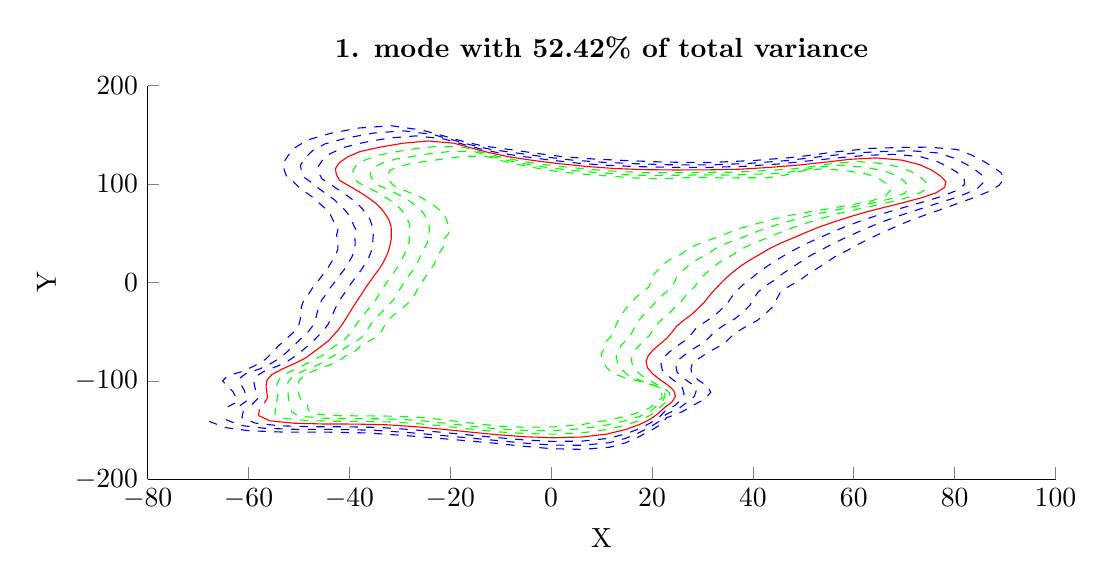
\begin{tikzpicture}

\begin{axis}[%
width=0.95092\figurewidth,
height=\figureheight,
at={(0\figurewidth,0\figureheight)},
scale only axis,
xmin=-80,
xmax=100,
xlabel={X},
ymin=-200,
ymax=200,
ylabel={Y},
title style={font=\bfseries},
title={1. mode with 52.42\% of total variance},
axis x line*=bottom,
axis y line*=left
]
\addplot [color=blue,dashed,forget plot]
  table[row sep=crcr]{%
-64.1113881531626	-126.422857227232\\
-62.3137493384501	-121.534773224667\\
-62.5526256797443	-116.293332766034\\
-63.0728549219847	-110.98018521314\\
-64.111403013549	-105.682726908696\\
-65.1322895148274	-100.031875030914\\
-64.1080439095626	-94.8104497674803\\
-61.1090411168025	-90.33972189999\\
-58.8295958909906	-84.7765929032281\\
-56.621062618512	-78.1549752094639\\
-55.3109326500943	-71.2982216786483\\
-54.0451785822157	-64.4681572170807\\
-52.6008484472825	-57.6923786737534\\
-51.1251964532574	-50.9116230843554\\
-50.0610191755853	-44.0599875699865\\
-49.7172223134401	-37.1191309253918\\
-49.6294508607351	-30.4876221921936\\
-49.4865806763933	-24.2260868148994\\
-49.0361965944735	-18.0145758621749\\
-48.0902034998486	-11.8668996644883\\
-47.2898383930681	-5.42269275190331\\
-46.3146828733534	0.690725553070188\\
-45.4186600369115	6.85423738676375\\
-44.4453716357019	12.9957785750946\\
-43.6828247766242	19.6201049927491\\
-42.7925591316775	26.6759664763406\\
-42.2893434869477	33.7738276724304\\
-42.2929514401841	40.9033038624999\\
-42.5306904422281	48.0347381765512\\
-42.215164164039	55.1473028052137\\
-43.1399711531593	62.2520905995861\\
-43.8175186741618	69.3200662393259\\
-44.8773821472101	75.5923960704164\\
-46.0958188496898	81.0627904289118\\
-47.2849655946893	86.6032465031828\\
-48.7799687820913	92.0853016737529\\
-50.1926773229734	97.5270334455254\\
-51.2514162544181	103.019816902071\\
-52.505406359378	108.498326512903\\
-52.9043463016658	114.051798955237\\
-53.1857590480468	120.8578270327\\
-52.1424654475473	128.871614371486\\
-50.7869231984063	136.863957499433\\
-48.3462903008677	144.613243273001\\
-43.7632784556929	151.448306014127\\
-38.0760626566901	156.899669468677\\
-31.6941907301334	159.182426797544\\
-25.6215339435526	154.752263983318\\
-21.5064958162697	149.125153683201\\
-17.8510640626736	143.774272712467\\
-13.6370281382769	138.742702345613\\
-8.22241503940673	135.045134317909\\
-2.97589621152903	131.182801803362\\
2.46521541859346	127.631918861494\\
8.55593505910047	125.348975265356\\
14.9677471658051	123.776088452363\\
22.6480359591807	122.218057265704\\
31.5649597008912	121.830150145465\\
40.3164634617137	123.920497372512\\
48.5660989353686	127.273172039313\\
55.9642530794155	132.373907759319\\
63.4140842903074	136.17276859077\\
68.9857411480043	137.06563826324\\
74.8289438848868	137.458024211548\\
80.497678140347	135.051565846542\\
83.3259225365914	129.465742973752\\
85.5753403547145	123.571323386359\\
87.5036686498257	117.622639474196\\
89.1775942156016	111.557729153636\\
89.7979922249149	105.225595884663\\
88.8436266197064	98.8692065058364\\
86.9224843303053	92.7257821860461\\
84.1645961294153	86.7891268580837\\
80.9568514023326	80.8783092294654\\
77.8180425112543	74.9913343219719\\
74.5239674780353	69.2198684963696\\
71.4035519556492	63.3174297815561\\
68.5650039576442	57.2552619589546\\
65.921730037945	51.1446770044502\\
63.3100045806704	45.0058087722051\\
60.9558733761274	38.8721003088333\\
58.8342087234764	32.8175330459414\\
56.4640176309109	26.8049211894389\\
54.684136723229	20.6481660800637\\
52.8443364257312	14.5229152880609\\
50.9033931859312	8.38183594041532\\
49.3366351683298	2.15210740813702\\
47.1312776959867	-4.04424070928949\\
45.3877990902005	-10.6179004353686\\
44.6296255325143	-17.70030978331\\
43.9404169584057	-24.8052686685917\\
42.4914875489309	-31.7290671870478\\
40.8721079654834	-38.6425065565061\\
38.4863249455975	-45.2928031107952\\
36.2956888269719	-51.944502245788\\
35.0103252320725	-58.733649647962\\
33.3608655968428	-64.9567805390354\\
31.2689247109958	-70.5133563116024\\
29.6665655595355	-76.0246157244469\\
28.0148262416386	-81.5907920368348\\
27.7246280580343	-87.7065677805129\\
27.9115724637363	-93.7173545678958\\
29.2780334192575	-99.6122267386532\\
30.9684451344403	-105.204106259172\\
31.6376496249636	-111.639369245924\\
30.3836726245072	-118.774045906247\\
27.9708838021748	-125.345469939367\\
26.0144789022887	-131.309562670408\\
22.8669424990321	-137.602461831795\\
21.821588953982	-144.233062467167\\
19.6540274372773	-150.708337660418\\
17.2816986468469	-157.133657648061\\
14.8379000278128	-162.840936080487\\
11.6255146635044	-167.426010238427\\
6.18167162546853	-169.648556876662\\
0.147745443773704	-168.950442183307\\
-5.60450349426934	-166.408802301064\\
-11.0949845407994	-163.421031128254\\
-16.7058794237253	-160.877311634416\\
-22.3835681934064	-158.374081318985\\
-28.9650090083777	-155.55222628904\\
-36.648433825369	-152.911218290289\\
-44.6619701957547	-152.086041473289\\
-52.7840220887422	-152.107995459061\\
-59.8823594667086	-150.721341196663\\
-64.4673179793973	-147.585298828544\\
-67.8759967645611	-141.084629166979\\
-67.3996678159056	-133.852446775627\\
};
\addplot [color=blue,dashed,forget plot]
  table[row sep=crcr]{%
-61.695953787725	-125.190245272256\\
-60.2785095200496	-120.001877428854\\
-60.499029811073	-114.537069946411\\
-60.8897946184	-109.025375623283\\
-61.5227966930159	-103.533483719334\\
-61.8663612794511	-97.8428166477487\\
-60.4962351438972	-92.52869353773\\
-57.7223996014046	-87.7474771787577\\
-55.4748746224303	-82.1951563481528\\
-53.4803691585979	-75.8313281646612\\
-52.0970672972122	-69.3045196228365\\
-50.7513035582749	-62.7968373030166\\
-49.436632050124	-56.2881836320302\\
-48.113093964095	-49.7732846043094\\
-47.1270919710259	-43.2023736575266\\
-46.6567932975192	-36.5659590044081\\
-46.3569104748883	-30.1337634944562\\
-46.0139004603166	-23.9437214493651\\
-45.4564764987152	-17.7885390958142\\
-44.5585151014238	-11.675896965039\\
-43.7824027724446	-5.34200988044179\\
-42.8480640920245	0.742082809289558\\
-41.9770437029931	6.86456060449893\\
-41.0291892967174	12.9674687481934\\
-40.2629689907632	19.4143894731556\\
-39.4647074098501	26.1699616175395\\
-38.9544445631107	32.9572466784999\\
-38.8475198696134	39.7697397192522\\
-38.9234564488773	46.583298213369\\
-38.7054308345703	53.3858219604455\\
-39.3314650166163	60.1807619792267\\
-39.8927201978543	66.9498097046236\\
-40.8241562195506	73.1647609632157\\
-41.9243984152409	78.822212560518\\
-43.1024182259622	84.5157467648869\\
-44.6232271030564	90.1386877709343\\
-46.1417130258015	95.7121346205963\\
-47.4897632465134	101.278064245981\\
-48.9700156485093	106.832128847318\\
-49.4605705436805	112.536623090926\\
-49.7141910150576	119.077165501048\\
-48.7603860531663	126.425230242263\\
-47.326226775564	133.718303652489\\
-44.8570935739479	140.729102111781\\
-40.4532863335107	146.807823225611\\
-35.1557409045002	151.748556472189\\
-29.2453570296226	154.021457357101\\
-23.5108276807479	150.327287011828\\
-19.6493287994099	144.994565694864\\
-16.0322589378425	139.841294287385\\
-11.8688156531972	135.007488703344\\
-6.65980646783072	131.329171075162\\
-1.47730350773011	127.680359530343\\
3.9163311717051	124.38778347422\\
9.84716346138721	122.15325615428\\
16.0821441618528	120.703079412113\\
23.2645650752419	119.560696493612\\
31.3500246577719	119.33467216787\\
39.2947803620665	120.941832603287\\
46.8219800041536	123.794693130317\\
53.7086636188151	128.012413289974\\
60.4865971466749	131.545258202766\\
65.7460525667162	133.074831731216\\
71.343651966029	133.793197302095\\
76.8244826431136	131.466121761116\\
79.9107159067882	126.188203024284\\
82.185109148888	120.429568148861\\
84.0345364531669	114.559347394768\\
85.5344700791069	108.571216568267\\
85.8782839517709	102.373849506604\\
84.6587148743309	96.2415215235617\\
82.3833633153951	90.4330798985261\\
79.380584431329	84.8619641249879\\
75.9987773815669	79.3543868155862\\
72.6959457588165	73.8387561658198\\
69.3887397271781	68.3205806004792\\
66.2703786821027	62.6642049838815\\
63.3886502701201	56.8719606805629\\
60.765944887241	50.9824808068347\\
58.196652052949	45.0598851679726\\
55.7664677909418	39.1298329647651\\
53.5953167256851	33.182818341779\\
51.3812401870955	27.2176597947584\\
49.5375434730962	21.170046104157\\
47.7297553910422	15.1186366033696\\
45.9378647480299	9.03181203400735\\
44.4502470750233	2.87266608017174\\
42.5858475357627	-3.26795604498727\\
41.0382330514492	-9.68633729784098\\
40.1843858497867	-16.4685438900365\\
39.4143434767987	-23.268198267261\\
38.0406812792055	-29.9306473489562\\
36.5412345499405	-36.5757637646053\\
34.4252683696823	-43.0057807380074\\
32.4882368316665	-49.4592674535257\\
31.3287871936452	-56.0329156505793\\
29.8872717247486	-62.2091721828549\\
28.0383399767467	-67.8999803410997\\
26.5125939084997	-73.5483335045536\\
25.0946225518787	-79.2331009325039\\
24.7563485766883	-85.3303208232274\\
24.9763862795279	-91.3764059415273\\
26.2131401193182	-97.3047828540775\\
27.8165250984406	-103.003828909168\\
28.8213819460206	-109.233643370574\\
28.373933141927	-115.878978703937\\
26.8662730785774	-122.167946625663\\
25.3255164833182	-128.045763824717\\
22.7282323097098	-134.168743235648\\
21.6229264589105	-140.530544096357\\
19.66282770234	-146.774556395601\\
17.3445949402049	-152.917992311551\\
14.7726599163733	-158.430466582955\\
11.4411198885411	-162.96525617167\\
6.16296256559745	-165.447949021523\\
0.236392197509329	-165.255821231626\\
-5.49160763123365	-163.202131904555\\
-10.986071274982	-160.513694214084\\
-16.4922044670727	-157.934156460588\\
-22.0169307448782	-155.349932066777\\
-28.2282027291598	-152.584303232174\\
-35.3104273503704	-150.148661605263\\
-42.7062482761098	-149.365544198106\\
-50.1969502058551	-149.35358048624\\
-56.8963117800344	-148.174200100347\\
-61.5658526577679	-145.259703148531\\
-64.5928503930024	-139.162708354565\\
-64.2119330958518	-132.216795295661\\
};
\addplot [color=blue,dashed,forget plot]
  table[row sep=crcr]{%
-59.2805194222875	-123.957633317281\\
-58.243269701649	-118.468981633041\\
-58.4454339424017	-112.780807126787\\
-58.7067343148152	-107.070566033426\\
-58.9341903724828	-101.384240529973\\
-58.6004330440747	-95.653758264583\\
-56.8844263782317	-90.2469373079798\\
-54.3357580860068	-85.1552324575255\\
-52.12015335387	-79.6137197930775\\
-50.3396756986837	-73.5076811198585\\
-48.8832019443302	-67.3108175670248\\
-47.4574285343342	-61.1255173889525\\
-46.2724156529655	-54.8839885903071\\
-45.1009914749325	-48.6349461242634\\
-44.1931647664665	-42.3447597450666\\
-43.5963642815983	-36.0127870834244\\
-43.0843700890415	-29.7799047967189\\
-42.54122024424	-23.6613560838309\\
-41.8767564029569	-17.5625023294536\\
-41.026826702999	-11.4848942655896\\
-40.2749671518211	-5.26132700898027\\
-39.3814453106955	0.793440065508928\\
-38.5354273690747	6.87488382223412\\
-37.6130069577328	12.9391589212921\\
-36.8431132049022	19.2086739535622\\
-36.1368556880227	25.6639567587384\\
-35.6195456392737	32.1406656845694\\
-35.4020882990427	38.6361755760044\\
-35.3162224555265	45.1318582501869\\
-35.1956975051017	51.6243411156772\\
-35.5229588800733	58.1094333588673\\
-35.9679217215468	64.5795531699213\\
-36.7709302918911	70.7371258560149\\
-37.752977980792	76.5816346921242\\
-38.9198708572351	82.4282470265911\\
-40.4664854240214	88.1920738681157\\
-42.0907487286295	93.8972357956671\\
-43.7281102386088	99.5363115898922\\
-45.4346249376405	105.165931181733\\
-46.0167947856952	111.021447226615\\
-46.2426229820684	117.296503969396\\
-45.3783066587853	123.97884611304\\
-43.8655303527216	130.572649805545\\
-41.3678968470282	136.844960950561\\
-37.1432942113284	142.167340437094\\
-32.2354191523103	146.597443475701\\
-26.7965233291118	148.860487916657\\
-21.4001214179431	145.902310040338\\
-17.7921617825502	140.863977706528\\
-14.2134538130113	135.908315862303\\
-10.1006031681176	131.272275061075\\
-5.09719789625471	127.613207832416\\
0.021289196068816	124.177917257324\\
5.36744692481674	121.143648086946\\
11.138391863674	118.957537043205\\
17.1965411579004	117.630070371863\\
23.8810941913031	116.90333572152\\
31.1350896146525	116.839194190276\\
38.2730972624193	117.963167834062\\
45.0778610729386	120.316214221321\\
51.4530741582148	123.650918820629\\
57.5591100030424	126.917747814762\\
62.506363985428	129.084025199191\\
67.8583600471711	130.128370392642\\
73.1512871458802	127.880677675689\\
76.4955092769851	122.910663074816\\
78.7948779430615	117.287812911362\\
80.5654042565081	111.496055315339\\
81.8913459426122	105.584703982899\\
81.9585756786268	99.5221031285463\\
80.4738031289553	93.613836541287\\
77.8442423004849	88.1403776110062\\
74.5965727332426	82.9348013918919\\
71.0407033608012	77.830464401707\\
67.5738490063788	72.6861780096677\\
64.253511976321	67.4212927045888\\
61.1372054085562	62.0109801862069\\
58.212296582596	56.4886594021711\\
55.6101597365369	50.8202846092192\\
53.0832995252277	45.11396156374\\
50.5770622057562	39.3875656206969\\
48.3564247278938	33.5481036376166\\
46.2984627432801	27.6303984000778\\
44.3909502229634	21.6919261282504\\
42.6151743563531	15.7143579186783\\
40.9723363101286	9.68178812759938\\
39.5638589817168	3.59322475220647\\
38.0404173755386	-2.49167138068506\\
36.688667012698	-8.75477416031335\\
35.739146167059	-15.236777996763\\
34.8882699951917	-21.7311278659303\\
33.5898750094802	-28.1322275108647\\
32.2103611343975	-34.5090209727044\\
30.3642117937671	-40.7187583652195\\
28.6807848363611	-46.9740326612634\\
27.647249155218	-53.3321816531967\\
26.4136778526545	-59.4615638266744\\
24.8077552424976	-65.2866043705969\\
23.3586222574638	-71.0720512846603\\
22.1744188621188	-76.875409828173\\
21.7880690953423	-82.954073865942\\
22.0412000953194	-89.0354573151589\\
23.148246819379	-94.9973389695018\\
24.664605062441	-100.803551559163\\
26.0051142670777	-106.827917495223\\
26.3641936593467	-112.983911501626\\
25.7616623549799	-118.99042331196\\
24.6365540643476	-124.781964979026\\
22.5895221203875	-130.7350246395\\
21.424263963839	-136.828025725547\\
19.6716279674027	-142.840775130784\\
17.4074912335629	-148.702326975042\\
14.7074198049339	-154.019997085423\\
11.2567251135777	-158.504502104913\\
6.14425350572636	-161.247341166383\\
0.325038951244953	-161.561200279945\\
-5.37871176819796	-159.995461508046\\
-10.8771580091646	-157.606357299913\\
-16.2785295104202	-154.99100128676\\
-21.6502932963501	-152.325782814569\\
-27.4913964499419	-149.616380175309\\
-33.9724208753718	-147.386104920238\\
-40.7505263564648	-146.645046922923\\
-47.609878322968	-146.599165513418\\
-53.9102640933602	-145.627059004031\\
-58.6643873361384	-142.934107468518\\
-61.3097040214437	-137.24078754215\\
-61.0241983757981	-130.581143815695\\
};
\addplot [color=red,solid,forget plot]
  table[row sep=crcr]{%
-56.8650850568499	-122.725021362305\\
-56.2080298832485	-116.936085837228\\
-56.3918380737305	-111.024544307164\\
-56.5236740112305	-105.115756443569\\
-56.3455840519496	-99.234997340611\\
-55.3345048086984	-93.4646998814174\\
-53.2726176125663	-87.9651810782296\\
-50.949116570609	-82.5629877362933\\
-48.7654320853097	-77.0322832380022\\
-47.1989822387695	-71.1840340750558\\
-45.6693365914481	-65.317115511213\\
-44.1635535103934	-59.4541974748884\\
-43.1081992558071	-53.479793548584\\
-42.0888889857701	-47.4966076442174\\
-41.2592375619071	-41.4871458326067\\
-40.5359352656773	-35.4596151624407\\
-39.8118297031948	-29.4260460989816\\
-39.0685400281634	-23.3789907182966\\
-38.2970363071987	-17.3364655630929\\
-37.4951383045741	-11.2938915661403\\
-36.7675315311977	-5.18064413751875\\
-35.9148265293666	0.844797321728298\\
-35.0938110351563	6.88520703996931\\
-34.1968246187483	12.9108490943909\\
-33.4232574190412	19.0029584339687\\
-32.8090039661952	25.1579518999372\\
-32.2846467154367	31.324084690639\\
-31.956656728472	37.5026114327567\\
-31.7089884621756	43.6804182870047\\
-31.685964175633	49.8628602709089\\
-31.7144527435303	56.038104738508\\
-32.0431232452393	62.209296635219\\
-32.7177043642317	68.3094907488142\\
-33.5815575463431	74.3410568237305\\
-34.737323488508	80.3407472882952\\
-36.3097437449864	86.2454599652972\\
-38.0397844314575	92.082336970738\\
-39.9664572307042	97.794558933803\\
-41.8992342267718	103.499733516148\\
-42.57301902771	109.506271362305\\
-42.7710549490792	115.515842437744\\
-41.9962272644043	121.532461983817\\
-40.4048339298793	127.426995958601\\
-37.8787001201085	132.960819789342\\
-33.8333020891462	137.526857648577\\
-29.3150974001203	141.446330479213\\
-24.3476896286011	143.699518476214\\
-19.2894151551383	141.477333068848\\
-15.9349947656904	136.733389718192\\
-12.3946486881801	131.975337437221\\
-8.33239068303789	127.537061418806\\
-3.53458932467869	123.897244589669\\
1.51988189986774	120.675474984305\\
6.81856267792838	117.899512699672\\
12.4296202659607	115.761817932129\\
18.3109381539481	114.557061331613\\
24.4976233073643	114.245974949428\\
30.9201545715332	114.343716212681\\
37.251414162772	114.984503064837\\
43.3337421417236	116.837735312326\\
49.1974846976144	119.289424351283\\
54.6316228594099	122.290237426758\\
59.2666754041399	125.093218667167\\
64.3730681283133	126.463543483189\\
69.4780916486468	124.295233590262\\
73.0803026471819	119.633123125349\\
75.4046467372349	114.146057673863\\
77.0962720598493	108.43276323591\\
78.2482218061175	102.598191397531\\
78.0388674054827	96.6703567504883\\
76.2888913835798	90.9861515590123\\
73.3051212855748	85.8476753234863\\
69.8125610351563	81.007638658796\\
66.0826293400356	76.3065419878278\\
62.4517522539411	71.5335998535156\\
59.1182842254639	66.5220048086984\\
56.0040321350098	61.3577553885324\\
53.0359428950718	56.1053581237793\\
50.4543745858329	50.6580884116037\\
47.9699469975063	45.1680379595075\\
45.3876566205706	39.6452982766288\\
43.1175327301025	33.9133889334542\\
41.2156852994646	28.0431370053973\\
39.2443569728306	22.2138061523438\\
37.500593321664	16.310079233987\\
36.0068078722273	10.3317642211914\\
34.6774708884103	4.3137834242412\\
33.4949872153146	-1.71538671638284\\
32.3391009739467	-7.82321102278573\\
31.2939064843314	-14.0050121034895\\
30.3621965135847	-20.1940574645996\\
29.1390687397548	-26.3338076727731\\
27.8794877188546	-32.4422781808036\\
26.3031552178519	-38.4317359924316\\
24.8733328410557	-44.4887978690011\\
23.9657111167908	-50.631447655814\\
22.9400839805603	-56.7139554704939\\
21.5771705082485	-62.6732284000942\\
20.2046506064279	-68.595769064767\\
19.2542151723589	-74.5177187238421\\
18.8197896139962	-80.5778269086565\\
19.106013911111	-86.6945086887905\\
20.0833535194397	-92.6898950849261\\
21.5126850264413	-98.6032742091588\\
23.1888465881348	-104.422191619873\\
24.3544541767665	-110.088844299316\\
24.6570516313825	-115.812899998256\\
23.947591645377	-121.518166133336\\
22.4508119310652	-127.301306043352\\
21.2256014687674	-133.125507354736\\
19.6804282324655	-138.906993865967\\
17.4703875269209	-144.486661638532\\
14.6421796934945	-149.609527587891\\
11.0723303386143	-154.043748038156\\
6.12554444585528	-157.046733311244\\
0.413685704980578	-157.866579328265\\
-5.26581590516227	-156.788791111537\\
-10.7682447433472	-154.699020385742\\
-16.0648545537676	-152.047846112932\\
-21.2836558478219	-149.30163356236\\
-26.7545901707241	-146.648457118443\\
-32.6344144003732	-144.623548235212\\
-38.7948044368199	-143.92454964774\\
-45.0228064400809	-143.844750540597\\
-50.924216406686	-143.079917907715\\
-55.7629220145089	-140.608511788504\\
-58.0265576498849	-135.318866729736\\
-57.8364636557443	-128.945492335728\\
};
\addplot [color=green,dashed,forget plot]
  table[row sep=crcr]{%
-54.4496506914123	-121.492409407329\\
-54.1727900648479	-115.403190041415\\
-54.3382422050592	-109.26828148754\\
-54.3406137076457	-103.160946853711\\
-53.7569777314165	-97.0857541512496\\
-52.068576573322	-91.2756414982518\\
-49.6608088469008	-85.6834248484794\\
-47.5624750552111	-79.970743015061\\
-45.4107108167494	-74.450846682927\\
-44.0582887788554	-68.8603870302531\\
-42.455471238566	-63.3234134554013\\
-40.8696784864526	-57.7828775608243\\
-39.9439828586486	-52.0755985068609\\
-39.0767864966077	-46.3582691641714\\
-38.3253103573477	-40.6295319201468\\
-37.4755062497564	-34.906443241457\\
-36.539289317348	-29.0721874012443\\
-35.5958598120867	-23.0966253527623\\
-34.7173162114404	-17.1104287967323\\
-33.9634499061493	-11.102888866691\\
-33.2600959105742	-5.09996126605723\\
-32.4482077480377	0.896154577947668\\
-31.6521947012378	6.8955302577045\\
-30.7806422797637	12.8825392674896\\
-30.0034016331802	18.7972429143752\\
-29.4811522443678	24.6519470411361\\
-28.9497477915997	30.5075036967085\\
-28.5112251579013	36.3690472895089\\
-28.1017544688248	42.2289783238226\\
-28.1762308461644	48.1013794261406\\
-27.9059466069873	53.9667761181486\\
-28.1183247689318	59.8390401005167\\
-28.6644784365722	65.8818556416134\\
-29.4101371118942	72.1004789553367\\
-30.5547761197808	78.2532475499993\\
-32.1530020659514	84.2988460624786\\
-33.9888201342856	90.2674381458089\\
-36.2048042227995	96.0528062777138\\
-38.363843515903	101.833535850563\\
-39.1292432697247	107.991095497994\\
-39.2994869160901	113.735180906092\\
-38.6141478700233	119.086077854594\\
-36.944137507037	124.281342111657\\
-34.3895033931887	129.076678628122\\
-30.523309966964	132.88637486006\\
-26.3947756479304	136.295217482725\\
-21.8988559280903	138.53854903577\\
-17.1787088923335	137.052356097358\\
-14.0778277488306	132.602801729856\\
-10.5758435633489	128.042359012139\\
-6.56417819795822	123.801847776537\\
-1.97198075310268	120.181281346923\\
3.01847460366666	117.173032711286\\
8.26967843104002	114.655377312398\\
13.7208486682474	112.566098821053\\
19.4253351499958	111.484052291363\\
25.1141524234255	111.588614177336\\
30.7052195284139	111.848238235087\\
36.2297310631248	112.005838295612\\
41.5896232105087	113.35925640333\\
46.941895237014	114.927929881938\\
51.7041357157774	117.662727038754\\
56.0269868228518	121.102412135142\\
60.8877762094555	122.798716573736\\
65.8048961514133	120.709789504836\\
69.6650960173788	116.355583175881\\
72.0144155314084	111.004302436364\\
73.6271398631905	105.369471156481\\
74.6050976696228	99.6116788121623\\
74.1191591323386	93.8186103724302\\
72.1039796382043	88.3584665767376\\
68.7660002706646	83.5549730359664\\
65.0285493370699	79.0804759257001\\
61.1245553192699	74.7826195739487\\
57.3296555015034	70.3810216973635\\
53.9830564746067	65.622716912808\\
50.8708588614633	60.7045305908578\\
47.8595892075477	55.7220568453875\\
45.2985894351288	50.4958922139882\\
42.8565944697849	45.222114355275\\
40.198251035385	39.9030309325606\\
37.8786407323112	34.2786742292918\\
36.1329078556492	28.4558756107167\\
34.0977637226979	22.7356861764371\\
32.3860122869749	16.9058005492957\\
31.041279434326	10.9817403147834\\
29.7910827951038	5.03434209627593\\
28.9495570550906	-0.939102052080629\\
27.9895349351955	-6.89164788525811\\
26.8486668016038	-12.773246210216\\
25.8361230319777	-18.6569870632689\\
24.6882624700294	-24.5353878346815\\
23.5486143033117	-30.3755353889027\\
22.2420986419367	-36.1447136196438\\
21.0658808457504	-42.0035630767388\\
20.2841730783635	-47.9307136584314\\
19.4664901084661	-53.9663471143133\\
18.3465857739994	-60.0598524295914\\
17.050678955392	-66.1194868448737\\
16.334011482599	-72.1600276195112\\
15.8515101326502	-78.2015799513711\\
16.1708277269026	-84.353560062422\\
17.0184602195004	-90.3824512003503\\
18.3607649904416	-96.4029968591543\\
20.3725789091918	-102.016465744523\\
22.3447146941863	-107.193777097006\\
23.5524409077851	-112.635376684553\\
23.2586292264065	-118.254367287645\\
22.3121017417428	-123.867587447205\\
21.0269389736959	-129.422988983926\\
19.6892284975282	-134.97321260115\\
17.5332838202788	-140.270996302023\\
14.5769395820551	-145.199058090359\\
10.887935563651	-149.582993971399\\
6.10683538598419	-152.846125456105\\
0.502332458716202	-154.171958376584\\
-5.15292004212657	-153.582120715029\\
-10.6593314775298	-151.791683471571\\
-15.8511795971151	-149.104690939105\\
-20.9170183992938	-146.277484310152\\
-26.0177838915062	-143.680534061577\\
-31.2964079253746	-141.860991550186\\
-36.839082517175	-141.204052372557\\
-42.4357345571938	-141.090335567776\\
-47.9381687200118	-140.532776811399\\
-52.8614566928795	-138.282916108491\\
-54.7434112783262	-133.396945917322\\
-54.6487289356905	-127.309840855762\\
};
\addplot [color=green,dashed,forget plot]
  table[row sep=crcr]{%
-52.0342163259747	-120.259797452353\\
-52.1375502464474	-113.870294245602\\
-52.2846463363879	-107.512018667917\\
-52.157553404061	-101.206137263854\\
-51.1683714108834	-94.9365109618881\\
-48.8026483379457	-89.0865831150861\\
-46.0490000812354	-83.4016686187292\\
-44.1758335398133	-77.3784982938288\\
-42.0559895481891	-71.8694101278517\\
-40.9175953189412	-66.5367399854504\\
-39.241605885684	-61.3297113995895\\
-37.5758034625119	-56.1115576467602\\
-36.7797664614901	-50.6714034651377\\
-36.0646840074452	-45.2199306841254\\
-35.3913831527883	-39.7719180076869\\
-34.4150772338354	-34.3532713204733\\
-33.2667489315012	-28.7183287035069\\
-32.1231795960101	-22.8142599872281\\
-31.1375961156821	-16.8843920303716\\
-30.4317615077245	-10.9118861672416\\
-29.7526602899508	-5.01927839459571\\
-28.9815889667088	0.947511834167038\\
-28.2105783673194	6.90585347543968\\
-27.3644599407792	12.8542294405884\\
-26.5835458473193	18.5915273947817\\
-26.1533005225404	24.145942182335\\
-25.6148488677627	29.690922702778\\
-25.0657935873307	35.2354831462612\\
-24.494520475474	40.7775383606405\\
-24.6664975166957	46.3398985813723\\
-24.0974404704443	51.8954474977892\\
-24.1935262926243	57.4687835658144\\
-24.6112525089127	63.4542205344127\\
-25.2387166774453	69.8599010869429\\
-26.3722287510537	76.1657478117035\\
-27.9962603869164	82.35223215966\\
-29.9378558371136	88.4525393208797\\
-32.4431512148949	94.3110536216246\\
-34.8284528050342	100.167338184978\\
-35.6854675117394	106.475919633683\\
-35.8279188831009	111.95451937444\\
-35.2320684756423	116.639693725371\\
-33.4834410841947	121.135688264712\\
-30.900306666269	125.192537466902\\
-27.2133178447817	128.245892071543\\
-23.4744538957405	131.144104486237\\
-19.4500222275795	133.377579595327\\
-15.0680026295287	132.627379125867\\
-12.2206607319709	128.47221374152\\
-8.75703843851776	124.109380587057\\
-4.79596571287855	120.066634134267\\
-0.409372181526671	116.465318104176\\
4.51706730746559	113.670590438268\\
9.72079418415166	111.411241925125\\
15.0120770705342	109.370379709978\\
20.5397321460434	108.411043251112\\
25.7306815394868	108.931253405244\\
30.4902844852945	109.352760257493\\
35.2080479634776	109.027173526387\\
39.8455042792937	109.880777494334\\
44.6863057764137	110.566435412593\\
48.7766485721449	113.035216650749\\
52.7872982415637	117.111605603118\\
57.4024842905977	119.133889664284\\
62.1317006541799	117.124345419409\\
66.2498893875756	113.078043226414\\
68.6241843255819	107.862547198865\\
70.1580076665317	102.306179077052\\
70.9619735331281	96.625166226794\\
70.1994508591946	90.9668639943721\\
67.9190678928287	85.7307815944629\\
64.2268792557544	81.2622707484465\\
60.2445376389835	77.1533131926042\\
56.1664812985042	73.2586971600695\\
52.2075587490657	69.2284435412115\\
48.8478287237496	64.7234290169176\\
45.7376855879168	60.0513057931832\\
42.6832355200236	55.3387555669957\\
40.1428042844248	50.3336960163726\\
37.7432419420635	45.2761907510425\\
35.0088454501994	40.1607635884924\\
32.6397487345199	34.6439595251294\\
31.0501304118338	28.8686142160361\\
28.9511704725651	23.2575662005305\\
27.2714312522858	17.5015218646044\\
26.0757509964247	11.6317164083755\\
24.9046947017973	5.75490076831066\\
24.4041268948665	-0.162817387778413\\
23.6399688964442	-5.96008474773049\\
22.4034271188761	-11.5414803169425\\
21.3100495503707	-17.1199166619382\\
20.2374562003041	-22.7369679965899\\
19.2177408877688	-28.3087925970019\\
18.1810420660215	-33.8576912468559\\
17.258428850445	-39.5183282844765\\
16.6026350399363	-45.2299796610487\\
15.992896236372	-51.2187387581328\\
15.1160010397503	-57.4464764590887\\
13.8967073043561	-63.6432046249805\\
13.4138077928392	-69.8023365151803\\
12.8832306513042	-75.8253329940857\\
13.2356415426942	-82.0126114360536\\
13.9535669195612	-88.0750073157746\\
15.208844954442	-94.2027195091498\\
17.5563112302489	-99.6107398691724\\
20.3349752116061	-104.298709894696\\
22.4478301841877	-109.457853370849\\
22.5696668074359	-114.990568441954\\
22.1733915524205	-120.433868851057\\
20.8282764786244	-125.720470613116\\
19.6980287625909	-131.039431336333\\
17.5961801136368	-136.055330965513\\
14.5116994706157	-140.788588592826\\
10.7035407886876	-145.122239904641\\
6.08812632611311	-148.645517600966\\
0.590979212451827	-150.477337424903\\
-5.04002417909088	-150.37545031852\\
-10.5504182117124	-148.884346557401\\
-15.6375046404625	-146.161535765277\\
-20.5503809507656	-143.253335057944\\
-25.2809776122883	-140.712611004712\\
-29.958401450376	-139.098434865161\\
-34.88336059753	-138.483555097374\\
-39.8486626743067	-138.335920594955\\
-44.9521210333376	-137.985635715083\\
-49.95999137125	-135.957320428478\\
-51.4602649067674	-131.475025104908\\
-51.4609942156367	-125.674189375796\\
};
\addplot [color=green,dashed,forget plot]
  table[row sep=crcr]{%
-49.6187819605372	-119.027185497377\\
-50.1023104280468	-112.337398449789\\
-50.2310504677166	-105.755755848294\\
-49.9744931004762	-99.2513276739971\\
-48.5797650903502	-92.7872677725266\\
-45.5367201025694	-86.8975247319205\\
-42.4371913155699	-81.119912388979\\
-40.7891920244155	-74.7862535725965\\
-38.7012682796288	-69.2879735727764\\
-37.776901859027	-64.2130929406477\\
-36.0277405328019	-59.3360093437778\\
-34.2819284385711	-54.4402377326961\\
-33.6155500643316	-49.2672084234146\\
-33.0525815182828	-44.0815922040794\\
-32.4574559482289	-38.914304095227\\
-31.3546482179145	-33.8000993994896\\
-29.9942085456544	-28.3644700057696\\
-28.6504993799334	-22.5318946216938\\
-27.5578760199239	-16.6583552640109\\
-26.9000731092997	-10.7208834677923\\
-26.2452246693273	-4.93859552313419\\
-25.5149701853799	0.998869090386408\\
-24.768962033401	6.91617669317487\\
-23.9482776017946	12.8259196136871\\
-23.1636900614583	18.3858118751882\\
-22.825448800713	23.6399373235338\\
-22.2799499439257	28.8743417088475\\
-21.62036201676	34.1019190030135\\
-20.8872864821232	39.3260983974583\\
-21.1567641872271	44.5784177366041\\
-20.2889343339013	49.8241188774298\\
-20.2687278163168	55.0985270311121\\
-20.5580265812532	61.0265854272119\\
-21.0672962429964	67.6193232185492\\
-22.1896813823266	74.0782480734076\\
-23.8395187078815	80.4056182568414\\
-25.8868915399416	86.6376404959506\\
-28.6814982069903	92.5693009655354\\
-31.2930620941655	98.5011405193931\\
-32.2416917537541	104.960743769372\\
-32.3563508501117	110.173857842789\\
-31.8499890812613	114.193309596148\\
-30.0227446613524	117.990034417768\\
-27.4111099393493	121.308396305683\\
-23.9033257225995	123.605409283027\\
-20.5541321435505	125.992991489749\\
-17.0011885270688	128.216610154883\\
-12.9572963667239	128.202402154377\\
-10.3634937151111	124.341625753183\\
-6.93823331368659	120.176402161975\\
-3.02775322779888	116.331420491998\\
1.15323639004934	112.74935486143\\
6.01566001126451	110.168148165249\\
11.1719099372633	108.167106537851\\
16.3033054728209	106.174660598902\\
21.6541291420911	105.338034210862\\
26.347210655548	106.273892633152\\
30.2753494421752	106.857282279898\\
34.1863648638304	106.048508757161\\
38.1013853480787	106.402298585338\\
42.4307163158133	106.204940943248\\
45.8491614285124	108.407706262745\\
49.5476096602756	113.120799071093\\
53.9171923717399	115.469062754831\\
58.4585051569465	113.538901333982\\
62.8346827577725	109.800503276946\\
65.2339531197553	104.720791961367\\
66.6888754698729	99.2428869976227\\
67.3188493966334	93.6386536414256\\
66.2797425860505	88.1151176163141\\
63.7341561474532	83.1030966121882\\
59.6877582408443	78.9695684609266\\
55.4605259408972	75.2261504595083\\
51.2084072777386	71.7347747461903\\
47.085461996628	68.0758653850594\\
43.7126009728925	63.8241411210272\\
40.6045123143703	59.3980809955087\\
37.5068818324995	54.955454288604\\
34.9870191337207	50.1714998187571\\
32.6298894143421	45.33026714681\\
29.8194398650138	40.4184962444242\\
27.4008567367287	35.009244820967\\
25.9673529680183	29.2813528213556\\
23.8045772224323	23.7794462246239\\
22.1568502175967	18.0972431799131\\
21.1102225585234	12.2816925019675\\
20.0183066084908	6.47545944034539\\
19.8586967346425	0.613467276523802\\
19.2904028576929	-5.02852161020286\\
17.9581874361485	-10.3097144236689\\
16.7839760687636	-15.5828462606076\\
15.7866499305787	-20.9385481584984\\
14.8868674722259	-26.242049805101\\
14.1199854901063	-31.570668874068\\
13.4509768551396	-37.0330934922143\\
12.9210970015091	-42.5292456636661\\
12.5193023642778	-48.4711304019523\\
11.8854163055012	-54.8331004885859\\
10.7427356533202	-61.1669224050872\\
10.4936041030793	-67.4446454108494\\
9.91495116995814	-73.4490860368002\\
10.3004553584857	-79.6716628096851\\
10.8886736196219	-85.7675634311989\\
12.0569249184423	-92.0024421591453\\
14.740043551306	-97.2050139938221\\
18.3252357290259	-101.403642692386\\
21.3432194605903	-106.280330057145\\
21.8807043884653	-111.726769596263\\
22.0346813630982	-117.000150254909\\
20.6296139835529	-122.017952242306\\
19.7068290276537	-127.105650071516\\
17.6590764069948	-131.839665629004\\
14.4464593591763	-136.378119095294\\
10.5191460137242	-140.661485837884\\
6.06941726624202	-144.444909745827\\
0.679625966187451	-146.782716473222\\
-4.92712831605519	-147.168779922011\\
-10.4415049458949	-145.97700964323\\
-15.42382968381	-143.218380591449\\
-20.1837435022374	-140.229185805736\\
-24.5441713330704	-137.744687947846\\
-28.6203949753773	-136.335878180135\\
-32.9276386778851	-135.763057822191\\
-37.2615907914196	-135.581505622133\\
-41.9660733466634	-135.438494618766\\
-47.0585260496205	-133.631724748465\\
-48.1771185352087	-129.553104292494\\
-48.2732594955829	-124.038537895829\\
};
\end{axis}
\end{tikzpicture}%
					\caption{Modus 1}
					\label{fig:mode1}
				\end{subfigure}
				\quad
				\begin{subfigure}{0.3\textwidth}
					\centering
					% This file was created by matlab2tikz.
% Minimal pgfplots version: 1.3
%
%The latest updates can be retrieved from
%  http://www.mathworks.com/matlabcentral/fileexchange/22022-matlab2tikz
%where you can also make suggestions and rate matlab2tikz.
%
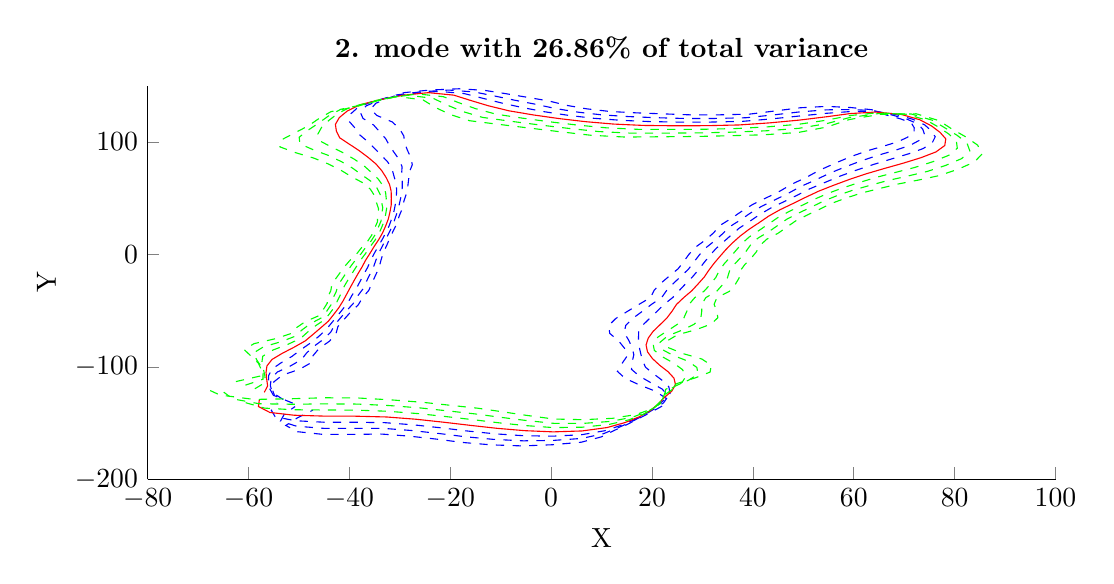
\begin{tikzpicture}

\begin{axis}[%
width=0.95092\figurewidth,
height=\figureheight,
at={(0\figurewidth,0\figureheight)},
scale only axis,
xmin=-80,
xmax=100,
xlabel={X},
ymin=-200,
ymax=150,
ylabel={Y},
title style={font=\bfseries},
title={2. mode with 26.86\% of total variance},
axis x line*=bottom,
axis y line*=left
]
\addplot [color=blue,dashed,forget plot]
  table[row sep=crcr]{%
-51.237496428345	-132.306429191379\\
-54.837895302831	-125.746779558981\\
-55.3116818197147	-119.638236139701\\
-54.9984568187473	-113.514007777185\\
-53.2918481777152	-107.476292254213\\
-49.8411444096922	-102.135661520003\\
-47.6259858748635	-96.4744565403381\\
-47.1950135148675	-90.0478566100794\\
-46.0004148884303	-83.6809247870241\\
-43.994267885798	-77.4177415502802\\
-42.681957895772	-70.9882045143104\\
-42.2715776927716	-64.2891583980012\\
-41.0470609884019	-57.8617472884963\\
-39.7796288878385	-51.4601325555301\\
-38.256875156468	-45.0658010482697\\
-37.3865275065577	-38.566825565018\\
-36.1495485340043	-32.0510039493923\\
-35.4956197976796	-25.4448600451726\\
-34.8329009195353	-18.8325032612857\\
-34.1421538554148	-12.2191533191379\\
-33.739720429412	-5.41392648976892\\
-33.2937021632905	1.24627387575211\\
-32.5986729352211	7.85883052726271\\
-31.9692254792386	14.4748922243818\\
-31.2756108181682	21.0201824649829\\
-30.5640222363394	27.4934942025311\\
-30.1275897668968	33.9934803770925\\
-29.522307633521	40.4831749797887\\
-29.2005228327323	46.9778238597622\\
-28.7215280833908	53.4908634438794\\
-28.4276814468144	60.0186869013027\\
-28.2503931047301	66.5610590684098\\
-28.1049437379711	73.0643511640457\\
-27.5315528619608	79.5661186418597\\
-27.7842087676806	85.9179952044755\\
-28.46684144728	92.2216634445774\\
-29.0129754659835	98.6199258619313\\
-29.2043513915178	105.156354784887\\
-30.0281406025594	111.489727698465\\
-31.508362280607	117.6752757445\\
-34.565672863084	123.442650469128\\
-35.7786437995241	129.065967472063\\
-34.7301376861289	134.338060334948\\
-32.1171985829835	139.084668253902\\
-29.1396804303774	143.719680301388\\
-24.0073991754087	146.027983036112\\
-18.2532925455601	147.146680112638\\
-13.186723161313	145.722581423731\\
-8.81978546142422	142.682973885501\\
-4.67931265163977	139.517051420121\\
-0.457806120812636	136.30822911191\\
3.06218815990746	132.415601842222\\
7.09770768439407	129.278938771853\\
11.757325960253	126.917920316784\\
16.8959605189458	125.742970995751\\
22.0001112380872	124.873990588642\\
27.3538273627714	124.007719645345\\
33.1633266327419	123.962149565738\\
39.2887639071291	124.586829562422\\
44.3643226691734	127.405079764588\\
49.3785732317037	130.26078728195\\
54.6393163637694	131.49295587718\\
59.4624410776368	130.444651842387\\
63.5828661861542	128.525188874977\\
66.5651529979239	123.68058896369\\
69.2661100265991	120.40889950213\\
71.4170547330251	116.737500600285\\
71.9863101605216	112.467698001653\\
71.9538226842193	108.099701476526\\
70.5759967012823	103.847897098785\\
68.6579182939331	99.9256479190053\\
66.0972409045662	96.3914593482645\\
62.7400682770787	92.1061355061849\\
59.2308388725044	86.5178280921385\\
56.1252213788145	80.5903172414704\\
53.1412691650042	74.5866859098471\\
50.5816506076375	68.3770730411122\\
47.7265519214741	62.3727027133486\\
45.3609707153151	56.1579760241694\\
42.6310140060618	50.1294262428922\\
39.9019365780968	44.1518568739769\\
37.6926410209359	37.9679949144444\\
35.6559831088956	31.7041921184617\\
33.4320176322701	25.5352459257526\\
32.2179455458339	19.0924641739258\\
30.5998410097536	12.7616420110911\\
28.6692753240574	6.47618769390898\\
27.3252221910563	-0.0175452352409367\\
26.2807138688838	-6.51107612054979\\
25.1736546993935	-12.9137828330392\\
23.4682292749759	-19.1968152787555\\
21.8215430619693	-25.4793207263126\\
20.4288136910112	-31.8818023767245\\
19.7398090448039	-38.3648715928242\\
17.4303530832423	-44.50008437191\\
15.116570125716	-50.7717559059185\\
12.8219464982875	-57.0629422949252\\
11.4144945936684	-63.3512147544528\\
11.6202312426282	-70.2572445861889\\
13.4653161395057	-77.461957443527\\
14.6564847761383	-84.1215076702343\\
15.0475489301832	-90.5259296161967\\
14.0510476182186	-97.1556742155422\\
13.1443611765652	-104.100616901956\\
14.6401691619273	-110.19201781471\\
17.1905836279883	-115.470035834047\\
20.7008103514596	-121.799986100245\\
22.8612970479534	-128.266103022013\\
22.2162549160568	-134.449445508923\\
19.8851330755916	-140.169810020679\\
17.4471398502664	-145.850154908393\\
15.0171455941603	-151.408928517207\\
12.4259563959661	-156.781571007306\\
9.99657249011388	-162.262059896417\\
5.98088962622012	-167.051399241424\\
0.326831235213677	-169.29309854708\\
-5.68491304669547	-170.358227333129\\
-11.8140217825475	-169.433369394829\\
-17.542528707116	-167.281688184281\\
-22.8428755697677	-164.246518071593\\
-28.1523463762454	-161.655377871128\\
-33.5892652629803	-159.813909566846\\
-39.3368392826369	-160.092731767597\\
-45.12818014801	-160.149215728213\\
-50.2494398755192	-157.733723842841\\
-52.6011986496772	-152.198073378327\\
-50.3551293519444	-145.567291300083\\
-47.2247251225459	-138.558468892801\\
};
\addplot [color=blue,dashed,forget plot]
  table[row sep=crcr]{%
-53.1133593045133	-129.112626581688\\
-55.2946068296368	-122.80988165173\\
-55.6717339043866	-116.767005528856\\
-55.506862549575	-110.71459066598\\
-54.3097601357933	-104.729193949679\\
-51.6722645426943	-99.2453409738078\\
-49.5081964540977	-93.6380313863019\\
-48.4463812001147	-87.5529003188173\\
-46.9220872873901	-81.4647109373501\\
-45.0625060034552	-75.3398390585387\\
-43.6777507943307	-69.0978415132779\\
-42.9022362986456	-62.6775047569636\\
-41.734107077537	-56.4010960418589\\
-40.5493822538157	-50.1389575850925\\
-39.2576626249477	-43.8729159763821\\
-38.4363300929309	-37.5310887641589\\
-37.3703089237345	-31.1760179992554\\
-36.6865932078409	-24.7562369362139\\
-35.9876127154231	-18.3338240285548\\
-35.2598153384679	-11.9107327348054\\
-34.7489907966739	-5.33616570568553\\
-34.1674102853159	1.11244835774417\\
-33.4303856351995	7.53428936483158\\
-32.7117585257418	13.9535445143848\\
-31.9914930184592	20.3477744546448\\
-31.3123494796247	26.7149801016665\\
-30.8466087497434	33.1036818149413\\
-30.333757331838	39.4896537974447\\
-30.0366780425468	45.8786886688431\\
-29.7096734474715	52.2815290528892\\
-29.523271879053	58.6918261803711\\
-29.5146364848998	65.1104715906796\\
-29.6425306133913	71.4793976923019\\
-29.5482210900882	77.8244313691499\\
-30.101913674623	84.0589125657488\\
-31.0811422131821	90.2295956181506\\
-32.0219117878081	96.4407295648669\\
-32.7917200045799	102.702422834526\\
-33.9851718106302	108.82639630436\\
-35.196581196308	114.952274283768\\
-37.3008002250824	120.800381125334\\
-37.8511716211508	126.554798975981\\
-36.6217031007124	132.034372209499\\
-34.0376990953585	137.043385432382\\
-30.7042209833003	141.655406083784\\
-25.7766319169793	144.500765517146\\
-20.2847582399071	145.99762623383\\
-15.2209538259214	144.30749863877\\
-11.1915218961796	140.699779163064\\
-7.25109133048655	137.003146759154\\
-3.08266764155439	133.384506547542\\
0.863262331712077	129.576149424704\\
5.23843242288529	126.411117509337\\
10.1110715328114	123.911784444414\\
15.4071804346174	122.415919974544\\
20.7703868767075	121.435014169632\\
26.4017593443024	120.753804746706\\
32.415602612339	120.756005114719\\
38.6096473256767	121.386054063227\\
44.0207958266901	123.882631613834\\
49.3182103870072	126.603666305061\\
54.6367518623162	128.425383060373\\
59.3971858531379	128.66084078398\\
63.8462668335406	127.837973744381\\
67.5361325481649	123.885470505881\\
70.5375075667934	120.150307376536\\
72.7462520677617	115.873686291477\\
73.6896307936308	111.122719746405\\
74.051955724852	106.265864783528\\
73.0636202693491	101.455383649353\\
71.201575990482	96.9458157990076\\
68.4998676982357	92.8768646733384\\
65.0975658631046	88.4066365570553\\
61.5147690283481	83.1140660573683\\
58.2340650038567	77.5714114454855\\
55.1336075184908	71.8984588761308\\
52.3891111167616	66.0373004902523\\
49.4963489126733	60.2835878501589\\
47.0587720054877	54.3246801533141\\
44.4106583365433	48.4756301484306\\
41.7305099255881	42.6496706748609\\
39.5009382573248	36.6164595874477\\
37.5092171724186	30.4838404141069\\
35.3694640791236	24.4280993346163\\
33.9788281377773	18.1650025272796\\
32.4021632972448	11.9516827477912\\
30.6720071788417	5.75538627068639\\
29.3818105324757	-0.583492395621573\\
28.3001762372381	-6.9484544212951\\
27.2137386277061	-13.2775259231893\\
25.7662183545122	-19.5292293407036\\
24.2607182878978	-25.7641497084661\\
22.9123717002923	-32.0686276447509\\
21.9275911024866	-38.3871597260267\\
19.9113463358468	-44.4963222042737\\
18.0662837894076	-50.724986489217\\
16.1946589923784	-56.9466133534481\\
14.8020532318617	-63.1252193029999\\
14.4817043638947	-69.7034194123816\\
15.3949491504568	-76.4805445369654\\
16.0442530554243	-82.9402807497084\\
16.4003705904925	-89.2487893070613\\
16.0618162519589	-95.6670811720035\\
15.9338024598572	-102.26816933769\\
17.4897283039964	-108.268742416431\\
19.5785404775811	-113.67630532247\\
22.0195574447673	-119.804290732915\\
23.2233952470946	-126.016790725787\\
22.2944405877263	-132.066732353733\\
20.3319558733169	-137.821709132031\\
18.1915693109994	-143.535767894251\\
15.8348929050805	-149.101506224316\\
13.1646974951423	-154.390889867501\\
10.355158439614	-159.52262261033\\
6.02910789943184	-163.716510598031\\
0.355782725135977	-165.484258807475\\
-5.54521399951774	-165.835081925932\\
-11.4654294361474	-164.521919725133\\
-17.0499706559999	-162.203740827165\\
-22.3231356624524	-159.264889901849\\
-27.6864276410716	-156.653070953567\\
-33.2709816421112	-154.750455789635\\
-39.1561610006979	-154.703337727645\\
-45.0930555787003	-154.714393999008\\
-50.4743653859081	-152.849121864466\\
-53.6551064379545	-148.33488618172\\
-52.9122721179246	-142.151149776634\\
-50.7619713002787	-135.354143373777\\
};
\addplot [color=blue,dashed,forget plot]
  table[row sep=crcr]{%
-54.9892221806816	-125.918823971996\\
-55.7513183564426	-119.872983744479\\
-56.0317859890585	-113.89577491801\\
-56.0152682804027	-107.915173554774\\
-55.3276720938715	-101.982095645145\\
-53.5033846756963	-96.3550204276126\\
-51.390407033332	-90.8016062322658\\
-49.6977488853618	-85.0579440275553\\
-47.8437596863499	-79.2484970876762\\
-46.1307441211124	-73.2619365667973\\
-44.6735436928894	-67.2074785122455\\
-43.5328949045195	-61.065851115926\\
-42.421153166672	-54.9404447952214\\
-41.3191356197929	-48.8177826146549\\
-40.2584500934274	-42.6800309044944\\
-39.4861326793041	-36.4953519632998\\
-38.5910693134646	-30.3010320491185\\
-37.8775666180021	-24.0676138272553\\
-37.1423245113109	-17.8351447958238\\
-36.377476821521	-11.6023121504728\\
-35.7582611639358	-5.25840492160214\\
-35.0411184073413	0.978622839736235\\
-34.2620983351779	7.20974820240044\\
-33.454291572245	13.4321968043878\\
-32.7073752187502	19.6753664443068\\
-32.06067672291	25.9364660008018\\
-31.56562773259	32.2138832527901\\
-31.145207030155	38.4961326151007\\
-30.8728332523612	44.7795534779239\\
-30.6978188115523	51.0721946618991\\
-30.6188623112916	57.3649654594395\\
-30.7788798650695	63.6598841129493\\
-31.1801174888115	69.894444220558\\
-31.5648893182157	76.0827440964402\\
-32.4196185815655	82.199829927022\\
-33.6954429790843	88.2375277917239\\
-35.0308481096328	94.2615332678024\\
-36.3790886176421	100.248490884164\\
-37.942203018701	106.163064910254\\
-38.884800112009	112.229272823036\\
-40.0359275870808	118.158111781539\\
-39.9236994427776	124.043630479899\\
-38.5132685152958	129.73068408405\\
-35.9581996077335	135.002102610862\\
-32.2687615362233	139.591131866181\\
-27.5458646585498	142.973547998179\\
-22.3162239342541	144.848572355022\\
-17.2551844905299	142.892415853809\\
-13.563258330935	138.716584440628\\
-9.82287000933333	134.489242098188\\
-5.70752916229614	130.460783983174\\
-1.33566349648331	126.736697007187\\
3.37915716137652	123.543296246821\\
8.46481710536991	120.905648572043\\
13.918400350289	119.088868953336\\
19.5406625153278	117.996037750622\\
25.4496913258333	117.499889848067\\
31.6678785919361	117.5498606637\\
37.9305307442244	118.185278564032\\
43.6772689842069	120.36018346308\\
49.2578475423108	122.946545328172\\
54.634187360863	125.357810243565\\
59.3319306286389	126.877029725573\\
64.1096674809269	127.150758613785\\
68.5071120984058	124.090352048071\\
71.8089051069877	119.891715250942\\
74.0754494024983	115.00987198267\\
75.3929514267401	109.777741491157\\
76.1500887654847	104.432028090529\\
75.5512438374159	99.0628701999205\\
73.7452336870309	93.9659836790099\\
70.9024944919053	89.3622699984124\\
67.4550634491304	84.7071376079256\\
63.7986991841918	79.7103040225981\\
60.3429086288989	74.5525056495006\\
57.1259458719773	69.2102318424146\\
54.1965716258857	63.6975279393923\\
51.2661459038726	58.1944729869691\\
48.7565732956603	52.4913842824589\\
46.1903026670248	46.8218340539691\\
43.5590832730793	41.1474844757448\\
41.3092354937137	35.264924260451\\
39.3624512359416	29.2634887097521\\
37.3069105259771	23.32095274348\\
35.7397107297206	17.2375408806333\\
34.204485584736	11.1417234844913\\
32.674739033626	5.03458484746379\\
31.4383988738951	-1.14943955600221\\
30.3196386055924	-7.38583272204042\\
29.2538225560188	-13.6412690133394\\
28.0642074340484	-19.8616434026516\\
26.6998935138263	-26.0489786906196\\
25.3959297095735	-32.2554529127772\\
24.1153731601692	-38.4094478592291\\
22.3923395884513	-44.4925600366374\\
21.0159974530992	-50.6782170725155\\
19.5673714864694	-56.830284411971\\
18.1896118700551	-62.899223851547\\
17.3431774851613	-69.1495942385743\\
17.3245821614078	-75.4991316304037\\
17.4320213347103	-81.7590538291824\\
17.7531922508017	-87.9716489979259\\
18.0725848856993	-94.1784881284648\\
18.7232437431493	-100.435721773425\\
20.3392874460656	-106.345467018152\\
21.9664973271738	-111.882574810893\\
23.3383045380749	-117.808595365586\\
23.5854934462358	-123.767478429561\\
22.3726262593957	-129.684019198543\\
20.7787786710421	-135.473608243384\\
18.9359987717324	-141.221380880109\\
16.6526402160007	-146.794083931424\\
13.9034385943184	-152.000208727696\\
10.7137443891142	-156.783185324243\\
6.07732617264356	-160.381621954638\\
0.384734215058277	-161.67541906787\\
-5.40551495234	-161.311936518735\\
-11.1168370897473	-159.610470055438\\
-16.5574126048837	-157.125793470049\\
-21.8033957551372	-154.283261732105\\
-27.2205089058978	-151.650764036005\\
-32.9526980212422	-149.687002012424\\
-38.9754827187589	-149.313943687692\\
-45.0579310093906	-149.279572269802\\
-50.6992908962971	-147.96451988609\\
-54.7090142262317	-144.471698985112\\
-55.4694148839048	-138.735008253185\\
-54.2992174780115	-132.149817854753\\
};
\addplot [color=red,solid,forget plot]
  table[row sep=crcr]{%
-56.8650850568499	-122.725021362305\\
-56.2080298832485	-116.936085837228\\
-56.3918380737305	-111.024544307164\\
-56.5236740112305	-105.115756443569\\
-56.3455840519496	-99.234997340611\\
-55.3345048086984	-93.4646998814174\\
-53.2726176125663	-87.9651810782296\\
-50.949116570609	-82.5629877362933\\
-48.7654320853097	-77.0322832380022\\
-47.1989822387695	-71.1840340750558\\
-45.6693365914481	-65.317115511213\\
-44.1635535103934	-59.4541974748884\\
-43.1081992558071	-53.479793548584\\
-42.0888889857701	-47.4966076442174\\
-41.2592375619071	-41.4871458326067\\
-40.5359352656773	-35.4596151624407\\
-39.8118297031948	-29.4260460989816\\
-39.0685400281634	-23.3789907182966\\
-38.2970363071987	-17.3364655630929\\
-37.4951383045741	-11.2938915661403\\
-36.7675315311977	-5.18064413751875\\
-35.9148265293666	0.844797321728298\\
-35.0938110351563	6.88520703996931\\
-34.1968246187483	12.9108490943909\\
-33.4232574190412	19.0029584339687\\
-32.8090039661952	25.1579518999372\\
-32.2846467154367	31.324084690639\\
-31.956656728472	37.5026114327567\\
-31.7089884621756	43.6804182870047\\
-31.685964175633	49.8628602709089\\
-31.7144527435303	56.038104738508\\
-32.0431232452393	62.209296635219\\
-32.7177043642317	68.3094907488142\\
-33.5815575463431	74.3410568237305\\
-34.737323488508	80.3407472882952\\
-36.3097437449864	86.2454599652972\\
-38.0397844314575	92.082336970738\\
-39.9664572307042	97.794558933803\\
-41.8992342267718	103.499733516148\\
-42.57301902771	109.506271362305\\
-42.7710549490792	115.515842437744\\
-41.9962272644043	121.532461983817\\
-40.4048339298793	127.426995958601\\
-37.8787001201085	132.960819789342\\
-33.8333020891462	137.526857648577\\
-29.3150974001203	141.446330479213\\
-24.3476896286011	143.699518476214\\
-19.2894151551383	141.477333068848\\
-15.9349947656904	136.733389718192\\
-12.3946486881801	131.975337437221\\
-8.33239068303789	127.537061418806\\
-3.53458932467869	123.897244589669\\
1.51988189986774	120.675474984305\\
6.81856267792838	117.899512699672\\
12.4296202659607	115.761817932129\\
18.3109381539481	114.557061331613\\
24.4976233073643	114.245974949428\\
30.9201545715332	114.343716212681\\
37.251414162772	114.984503064837\\
43.3337421417236	116.837735312326\\
49.1974846976144	119.289424351283\\
54.6316228594099	122.290237426758\\
59.2666754041399	125.093218667167\\
64.3730681283133	126.463543483189\\
69.4780916486468	124.295233590262\\
73.0803026471819	119.633123125349\\
75.4046467372349	114.146057673863\\
77.0962720598493	108.43276323591\\
78.2482218061175	102.598191397531\\
78.0388674054827	96.6703567504883\\
76.2888913835798	90.9861515590123\\
73.3051212855748	85.8476753234863\\
69.8125610351563	81.007638658796\\
66.0826293400356	76.3065419878278\\
62.4517522539411	71.5335998535156\\
59.1182842254639	66.5220048086984\\
56.0040321350098	61.3577553885324\\
53.0359428950718	56.1053581237793\\
50.4543745858329	50.6580884116037\\
47.9699469975063	45.1680379595075\\
45.3876566205706	39.6452982766288\\
43.1175327301025	33.9133889334542\\
41.2156852994646	28.0431370053973\\
39.2443569728306	22.2138061523438\\
37.500593321664	16.310079233987\\
36.0068078722273	10.3317642211914\\
34.6774708884103	4.3137834242412\\
33.4949872153146	-1.71538671638284\\
32.3391009739467	-7.82321102278573\\
31.2939064843314	-14.0050121034895\\
30.3621965135847	-20.1940574645996\\
29.1390687397548	-26.3338076727731\\
27.8794877188546	-32.4422781808036\\
26.3031552178519	-38.4317359924316\\
24.8733328410557	-44.4887978690011\\
23.9657111167908	-50.631447655814\\
22.9400839805603	-56.7139554704939\\
21.5771705082485	-62.6732284000942\\
20.2046506064279	-68.595769064767\\
19.2542151723589	-74.5177187238421\\
18.8197896139962	-80.5778269086565\\
19.106013911111	-86.6945086887905\\
20.0833535194397	-92.6898950849261\\
21.5126850264413	-98.6032742091588\\
23.1888465881348	-104.422191619873\\
24.3544541767665	-110.088844299316\\
24.6570516313825	-115.812899998256\\
23.947591645377	-121.518166133336\\
22.4508119310652	-127.301306043352\\
21.2256014687674	-133.125507354736\\
19.6804282324655	-138.906993865967\\
17.4703875269209	-144.486661638532\\
14.6421796934945	-149.609527587891\\
11.0723303386143	-154.043748038156\\
6.12554444585528	-157.046733311244\\
0.413685704980578	-157.866579328265\\
-5.26581590516227	-156.788791111537\\
-10.7682447433472	-154.699020385742\\
-16.0648545537676	-152.047846112932\\
-21.2836558478219	-149.30163356236\\
-26.7545901707241	-146.648457118443\\
-32.6344144003732	-144.623548235212\\
-38.7948044368199	-143.92454964774\\
-45.0228064400809	-143.844750540597\\
-50.924216406686	-143.079917907715\\
-55.7629220145089	-140.608511788504\\
-58.0265576498849	-135.318866729736\\
-57.8364636557443	-128.945492335728\\
};
\addplot [color=green,dashed,forget plot]
  table[row sep=crcr]{%
-58.7409479330182	-119.531218752613\\
-56.6647414100543	-113.999187929977\\
-56.7518901584024	-108.153313696318\\
-57.0320797420582	-102.316339332363\\
-57.3634960100278	-96.4878990360772\\
-57.1656249417004	-90.5743793352222\\
-55.1548281918005	-85.1287559241935\\
-52.2004842558561	-80.0680314450312\\
-49.6871044842695	-74.8160693883283\\
-48.2672203564267	-69.1061315833144\\
-46.6651294900068	-63.4267525101806\\
-44.7942121162673	-57.8425438338508\\
-43.7952453449421	-52.0191423019465\\
-42.8586423517473	-46.1754326737798\\
-42.2600250303868	-40.2942607607191\\
-41.5857378520505	-34.4238783615816\\
-41.0325900929249	-28.5510601488447\\
-40.2595134383246	-22.6903676093379\\
-39.4517481030864	-16.837786330362\\
-38.6127997876273	-10.9854709818078\\
-37.7768018984596	-5.10288335343536\\
-36.788534651392	0.71097180372036\\
-35.9255237351346	6.56066587753817\\
-34.9393576652515	12.3895013843939\\
-34.1391396193323	18.3305504236306\\
-33.5573312094805	24.3794377990726\\
-33.0036656982833	30.4342861284878\\
-32.768106426789	36.5090902504127\\
-32.5451436719901	42.5812830960856\\
-32.6741095397138	48.6535258799187\\
-32.8100431757689	54.7112440175764\\
-33.307366625409	60.7587091574888\\
-34.2552912396519	66.7245372770703\\
-35.5982257744706	72.5993695510207\\
-37.0550283954504	78.4816646495684\\
-38.9240445108885	84.2533921388704\\
-41.0487207532822	89.9031406736736\\
-43.5538258437663	95.3406269834416\\
-45.8562654348425	100.836402122042\\
-46.261237943411	106.783269901573\\
-45.5061823110777	112.873573093949\\
-44.068755086031	119.021293487735\\
-42.2963993444628	125.123307833152\\
-39.7992006324834	130.919536967821\\
-35.3978426420692	135.462583430973\\
-31.0843301416909	139.919112960247\\
-26.3791553229481	142.550464597406\\
-21.3236458197467	140.062250283886\\
-18.3067312004458	134.750194995756\\
-14.9664273670269	129.461432776254\\
-10.9572522037796	124.613338854438\\
-5.73351515287408	121.057792172152\\
-0.339393361641038	117.807653721789\\
5.17230825048685	114.893376827301\\
10.9408401816323	112.434766910921\\
17.0812137925684	111.118084912603\\
23.5455552888953	110.992060050789\\
30.1724305511303	111.137571761663\\
36.5722975813197	111.783727565642\\
42.9902152992404	113.315287161571\\
49.137121852918	115.632303374395\\
54.6290583579567	119.22266460995\\
59.201420179641	123.30940760876\\
64.6364687756997	125.776328352593\\
70.4490711988877	124.500115132453\\
74.3517001873762	119.374530999755\\
76.7338440719715	113.282243365056\\
78.7995926929586	107.087784980662\\
80.3463548467502	100.764354704532\\
80.5264909735495	94.2778433010561\\
78.8325490801287	88.0063194390146\\
75.7077480792443	82.3330806485603\\
72.1700586211821	77.3081397096664\\
68.3665594958793	72.9027799530576\\
64.5605958789833	68.5146940575307\\
61.1106225789504	63.8337777749822\\
57.8114926441339	59.0179828376724\\
54.8057398862711	54.0162432605895\\
52.1521758760055	48.8247925407484\\
49.7495913279878	43.514241865046\\
47.2162299680618	38.1431120775127\\
44.9258299664914	32.5618536064575\\
43.0689193629876	26.8227853010425\\
41.1818034196842	21.1066595612075\\
39.2614759136073	15.3826175873407\\
37.8091301597185	9.52180495789151\\
36.6802027431946	3.59298200101861\\
35.551575556734	-2.28133387676348\\
34.358563342301	-8.26058932353105\\
33.333990412644	-14.3687551936396\\
32.6601855931209	-20.5264715265476\\
31.5782439656833	-26.6186366549266\\
30.3630457281358	-32.6291034488299\\
28.4909372755346	-38.4540241256341\\
27.3543260936602	-44.4850357013648\\
26.9154247804823	-50.5846782391125\\
26.3127964746512	-56.5976265290167\\
24.9647291464418	-62.4472329486413\\
23.0661237276944	-68.0419438909597\\
21.18384818331	-73.5363058172805\\
20.2075578932822	-79.3965999881306\\
20.4588355714203	-85.4173683796551\\
22.0941221531801	-91.2013020413874\\
24.3021263097334	-96.7708266448929\\
26.0384057302039	-102.498916221594\\
26.7424110263593	-108.295113787739\\
25.9757987246902	-113.817204630927\\
24.3096898445182	-119.26885383711\\
22.5289976027346	-124.918592888162\\
21.6724242664927	-130.777406466089\\
20.4248576931985	-136.592606851825\\
18.2881348378411	-142.179239345641\\
15.3809207926707	-147.218846448086\\
11.4309162881145	-151.304310752069\\
6.173762719067	-153.711844667851\\
0.442637194902878	-154.057739588659\\
-5.12611685798453	-152.26564570434\\
-10.4196523969471	-149.787570716047\\
-15.5722965026515	-146.969898755816\\
-20.7639159405067	-144.320005392616\\
-26.2886714355503	-141.646150200881\\
-32.3161307795042	-139.560094458001\\
-38.6141261548809	-138.535155607788\\
-44.9876818707712	-138.409928811392\\
-51.1491419170749	-138.195315929339\\
-56.8168298027862	-136.745324591897\\
-60.5837004158651	-131.902725206288\\
-61.3737098334771	-125.741166816704\\
};
\addplot [color=green,dashed,forget plot]
  table[row sep=crcr]{%
-60.6168108091864	-116.337416142922\\
-57.1214529368601	-111.062290022726\\
-57.1119422430743	-105.282083085472\\
-57.5404854728859	-99.5169222211574\\
-58.381407968106	-93.7408007315433\\
-58.9967450747025	-87.684058789027\\
-57.0370387710348	-82.2923307701573\\
-53.4518519411033	-77.5730751537692\\
-50.6087768832293	-72.5998555386544\\
-49.3354584740839	-67.0282290915729\\
-47.6609223885655	-61.5363895091481\\
-45.4248707221413	-56.2308901928132\\
-44.4822914340772	-50.5584910553091\\
-43.6283957177245	-44.8542577033422\\
-43.2608124988665	-39.1013756888314\\
-42.6355404384237	-33.3881415607225\\
-42.253350482655	-27.6760741987078\\
-41.4504868484859	-22.0017445003793\\
-40.6064598989742	-16.3391070976311\\
-39.7304612706804	-10.6770503974753\\
-38.7860722657214	-5.02512256935196\\
-37.6622427734174	0.577146285712423\\
-36.7572364351131	6.23612471510704\\
-35.6818907117547	11.8681536743969\\
-34.8550218196233	17.6581424132925\\
-34.3056584527658	23.600923698208\\
-33.7226846811299	29.5444875663366\\
-33.579556125106	35.5155690680687\\
-33.3812988818045	41.4821479051664\\
-33.6622549037945	47.4441914889286\\
-33.9056336080075	53.3843832966448\\
-34.5716100055787	59.3081216797585\\
-35.7928781150721	65.1395838053265\\
-37.614894002598	70.857682278311\\
-39.3727333023929	76.6225820108417\\
-41.5383452767907	82.2613243124437\\
-44.0576570751069	87.7239443766091\\
-47.1411944568284	92.8866950330802\\
-49.8132966429133	98.1730707279368\\
-49.9494568591119	104.060268440841\\
-48.2413096730761	110.231303750155\\
-46.1412829076578	116.510124991653\\
-44.1879647590463	122.819619707702\\
-41.7197011448584	128.878254146301\\
-36.9623831949921	133.39830921337\\
-32.8535628832614	138.391895441281\\
-28.4106210172951	141.401410718598\\
-23.3578764843552	138.647167498925\\
-20.6784676352012	132.76700027332\\
-17.5382060458737	126.947528115288\\
-13.5821137245214	121.689616290069\\
-7.93244098106946	118.218339754635\\
-2.19866862314981	114.939832459274\\
3.52605382304532	111.887240954931\\
9.45206009730398	109.107715889714\\
15.8514894311887	107.679108493593\\
22.5934872704263	107.73814515215\\
29.4247065307274	107.931427310644\\
35.8931809998673	108.582952066447\\
42.6466884567572	109.792839010817\\
49.0767590082216	111.975182397506\\
54.6264938565036	116.155091793143\\
59.136164955142	121.525596550353\\
64.8998694230861	125.089113221997\\
71.4200507491286	124.704996674644\\
75.6230977275705	119.115938874162\\
78.0630414067081	112.418429056249\\
80.5029133260678	105.742806725414\\
82.4444878873829	98.9305180115337\\
83.0141145416163	91.8853298516239\\
81.3762067766776	85.0264873190169\\
78.1103748729138	78.8184859736342\\
74.5275562072079	73.6086407605368\\
70.650489651723	69.4990179182874\\
66.6694395040255	65.4957882615458\\
63.102960932437	61.1455507412659\\
59.6189531532579	56.6782102868125\\
56.5755368774704	51.9271283973997\\
53.8499771661781	46.9914966698932\\
51.5292356584692	41.8604457705845\\
49.0448033155531	36.6409258783967\\
46.7341272028803	31.2103182794608\\
44.9221534265106	25.6024335966877\\
43.1192498665377	19.9995129700712\\
41.0223585055507	14.4551559406944\\
39.6114524472097	8.71184569459161\\
38.6829345979789	2.87218057779602\\
37.6081638981535	-2.84728103714412\\
36.3780257106553	-8.69796762427636\\
35.3740743409567	-14.7324982837896\\
34.9581746726572	-20.8588855884957\\
34.0174191916118	-26.9034656370801\\
32.8466037374169	-32.8159287168563\\
30.6787193332173	-38.4763122588366\\
29.8353193462647	-44.4812735337286\\
29.8651384441739	-50.537908822411\\
29.6855089687422	-56.4812975875396\\
28.3522877846352	-62.2212374971884\\
25.927596848961	-67.4881187171525\\
23.1134811942611	-72.5548929107188\\
21.5953261725682	-78.2153730676047\\
21.8116572317296	-84.1402280705196\\
24.1048907869205	-89.7127089978486\\
27.0915675930254	-94.938379080627\\
28.8879648722731	-100.575640823315\\
29.130367875952	-106.501383276162\\
27.2945458179978	-111.821509263597\\
24.6717880436594	-117.019541540884\\
22.607183274404	-122.535879732972\\
22.119247064218	-128.429305577441\\
21.1692871539315	-134.278219837683\\
19.1058821487613	-139.871817052749\\
16.1196618918468	-144.82816530828\\
11.7895022376146	-148.564873465982\\
6.22198099227871	-150.376956024458\\
0.471588684825178	-150.248899849054\\
-4.98641781080679	-147.742500297143\\
-10.071060050547	-144.876121046351\\
-15.0797384515354	-141.8919513987\\
-20.2441760331914	-139.338377222872\\
-25.8227527003765	-136.64384328332\\
-31.9978471586351	-134.496640680789\\
-38.4334478729419	-133.145761567835\\
-44.9525573014616	-132.975107082187\\
-51.3740674274638	-133.310713950964\\
-57.8707375910634	-132.882137395289\\
-63.1408431818452	-128.486583682839\\
-64.9109560112099	-122.536841297679\\
};
\addplot [color=green,dashed,forget plot]
  table[row sep=crcr]{%
-62.4926736853547	-113.14361353323\\
-57.5781644636659	-108.125392115475\\
-57.4719943277463	-102.410852474626\\
-58.0488912037137	-96.7175051099518\\
-59.3993199261841	-90.9937024270095\\
-60.8278652077045	-84.7937382428318\\
-58.919249350269	-79.4559056161212\\
-54.7032196263504	-75.0781188625071\\
-51.5304492821891	-70.3836416889804\\
-50.4036965917411	-64.9503265998314\\
-48.6567152871242	-59.6460265081157\\
-46.0555293280152	-54.6192365517755\\
-45.1693375232122	-49.0978398086717\\
-44.3981490837017	-43.5330827329046\\
-44.2615999673462	-37.9084906169437\\
-43.6853430247969	-32.3524047598634\\
-43.4741108723852	-26.8010882485709\\
-42.6414602586471	-21.3131213914206\\
-41.761171694862	-15.8404278649001\\
-40.8481227537335	-10.3686298131427\\
-39.7953426329833	-4.94736178526857\\
-38.5359508954428	0.443320767704485\\
-37.5889491350914	5.91158355267591\\
-36.4244237582579	11.3468059644\\
-35.5709040199143	16.9857344029544\\
-35.0539856960511	22.8224095973434\\
-34.4417036639766	28.6546890041854\\
-34.391005823423	34.5220478857247\\
-34.217454091619	40.3830127142473\\
-34.6504002678753	46.2348570979384\\
-35.0012240402462	52.0575225757132\\
-35.8358533857484	57.8575342020282\\
-37.3304649904923	63.5546303335826\\
-39.6315622307255	69.1159950056012\\
-41.6904382093353	74.7634993721149\\
-44.1526460426928	80.269256486017\\
-47.0665933969316	85.5447480795447\\
-50.7285630698905	90.4327630827189\\
-53.7703278509841	95.5097393338311\\
-53.6376757748129	101.33726698011\\
-50.9764370350745	107.58903440636\\
-48.2138107292845	113.998956495571\\
-46.0795301736298	120.515931582253\\
-43.6402016572334	126.836971324781\\
-38.5269237479151	131.334034995766\\
-34.6227956248319	136.864677922314\\
-30.4420867116421	140.25235683979\\
-25.3921071489636	137.232084713964\\
-23.0502040699566	130.783805550883\\
-20.1099847247204	124.433623454321\\
-16.2069752452632	118.765893725701\\
-10.1313668092649	115.378887337117\\
-4.05794388465859	112.072011196758\\
1.87979939560379	108.88110508256\\
7.96328001297562	105.780664868507\\
14.621765069809	104.240132074584\\
21.6414192519573	104.484230253511\\
28.6769825103246	104.725282859625\\
35.214064418415	105.382176567252\\
42.3031616142739	106.270390860063\\
49.0163961635251	108.318061420617\\
54.6239293550504	113.087518976335\\
59.070909730643	119.741785491946\\
65.1632700704725	124.401898091401\\
72.3910302993696	124.909878216835\\
76.8944952677647	118.857346748568\\
79.3922387414447	111.554614747441\\
82.2062339591771	104.397828470166\\
84.5426209280157	97.0966813185352\\
85.5017381096832	89.4928164021917\\
83.9198644732265	82.0466551990193\\
80.5130016665833	75.3038912987082\\
76.8850537932338	69.9091418114072\\
72.9344198075668	66.0952558835172\\
68.7782831290677	62.4768824655608\\
65.0952992859235	58.4573237075497\\
61.426413662382	54.3384377359525\\
58.3453338686696	49.8380135342099\\
55.5477784563506	45.158200799038\\
53.3088799889507	40.2066496761229\\
50.8733766630443	35.1387396792806\\
48.5424244392692	29.8587829524641\\
46.7753874900336	24.3820818923329\\
45.0566963133912	18.8923663789349\\
42.7832410974941	13.5276942940481\\
41.4137747347009	7.90188643129172\\
40.6856664527632	2.15137915457343\\
39.6647522395729	-3.41322819752475\\
38.3974880790096	-9.13534592502167\\
37.4141582692693	-15.0962413739397\\
37.2561637521935	-21.1912996504437\\
36.4565944175403	-27.1882946192336\\
35.3301617466981	-33.0027539848826\\
32.8665013908999	-38.4986003920391\\
32.3163125988692	-44.4775113660923\\
32.8148521078655	-50.4911394057095\\
33.0582214628331	-56.3649686460625\\
31.7398464228285	-61.9952420457355\\
28.7890699702276	-66.9342935433452\\
25.0431142052121	-71.5734800041572\\
22.9830944518541	-77.0341461470788\\
23.1644788920389	-82.8630877613842\\
26.1156594206608	-88.2241159543099\\
29.8810088763174	-93.1059315163612\\
31.7375240143423	-98.6523654250364\\
31.5183247255447	-104.707652764585\\
28.6132929113055	-109.825813896268\\
25.0338862428006	-114.770229244659\\
22.6853689460735	-120.153166577782\\
22.5660698619433	-126.081204688794\\
21.9137166146646	-131.96383282354\\
19.9236294596815	-137.564394759857\\
16.8584029910229	-142.437484168475\\
12.1480881871148	-145.825436179895\\
6.27019926549043	-147.042067381065\\
0.500540174747478	-146.440060109449\\
-4.84671876362906	-143.219354889945\\
-9.72246770414686	-139.964671376655\\
-14.5871804004193	-136.814004041584\\
-19.7244361258762	-134.356749053128\\
-25.3568339652027	-131.641536365758\\
-31.6795635377661	-129.433186903578\\
-38.2527695910029	-127.756367527883\\
-44.9174327321519	-127.540285352981\\
-51.5989929378527	-128.426111972588\\
-58.9246453793406	-129.018950198682\\
-65.6979859478254	-125.07044215939\\
-68.4482021889427	-119.332515778655\\
};
\end{axis}
\end{tikzpicture}%
					\caption{Modus 2}
					\label{fig:mode2}
				\end{subfigure}	
				\quad
				\begin{subfigure}{0.3\textwidth}
					\centering
					% This file was created by matlab2tikz.
% Minimal pgfplots version: 1.3
%
%The latest updates can be retrieved from
%  http://www.mathworks.com/matlabcentral/fileexchange/22022-matlab2tikz
%where you can also make suggestions and rate matlab2tikz.
%
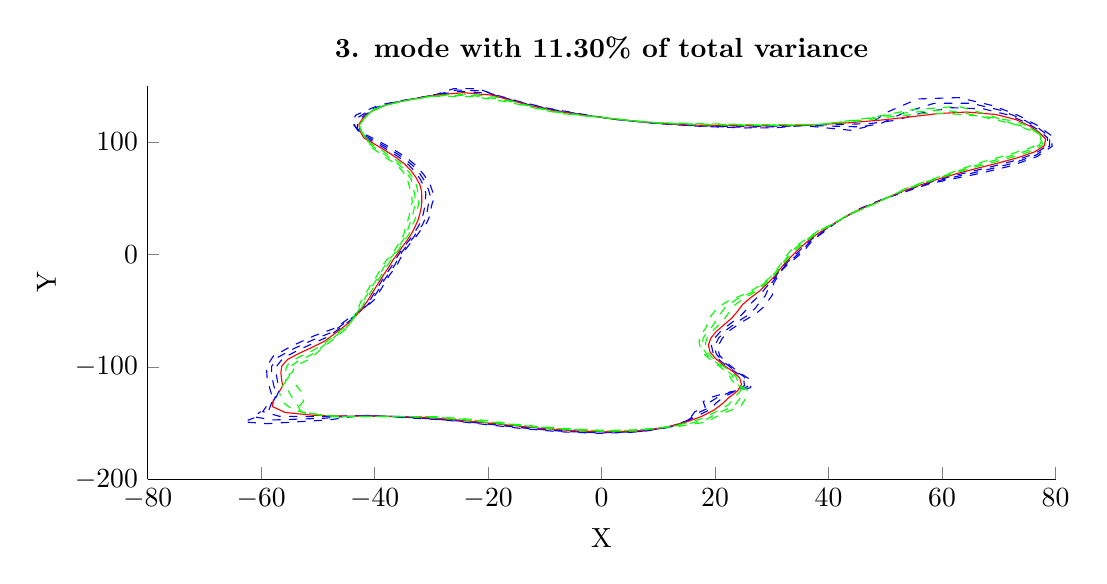
\begin{tikzpicture}

\begin{axis}[%
width=0.95092\figurewidth,
height=\figureheight,
at={(0\figurewidth,0\figureheight)},
scale only axis,
xmin=-80,
xmax=80,
xlabel={X},
ymin=-200,
ymax=150,
ylabel={Y},
title style={font=\bfseries},
title={3. mode with 11.30\% of total variance},
axis x line*=bottom,
axis y line*=left
]
\addplot [color=blue,dashed,forget plot]
  table[row sep=crcr]{%
-58.6193737057297	-138.319078758578\\
-57.9107399384524	-128.915981046782\\
-58.47129624748	-119.25995705236\\
-58.9445132537055	-109.58557369946\\
-59.0644072854577	-99.9520986208768\\
-57.8275555716103	-90.4235679551065\\
-54.5545021779963	-81.4050173407602\\
-50.7047534483931	-72.5850675944657\\
-47.2994914401819	-66.2570407498866\\
-45.9164279719243	-62.0280191429283\\
-44.7594459689413	-57.7258101973952\\
-43.4618252182764	-53.4708480541968\\
-42.2892015303312	-49.1601230274391\\
-41.0734202519053	-44.8494534194394\\
-40.0678885071914	-40.4998763957307\\
-39.5054603811978	-36.0809365066156\\
-38.8058483857283	-30.5650694873807\\
-38.0789943444387	-23.931571465913\\
-37.206335405946	-17.3188296548096\\
-36.1439815487927	-10.7230536207987\\
-35.5735062120769	-4.81802399161592\\
-34.9260031960005	1.82116607438277\\
-33.91973868042	8.42717952880677\\
-32.7923339887583	15.0072460122408\\
-31.9767951506978	20.782099370277\\
-31.0683359765831	25.7009998216671\\
-30.5590953392998	30.6612470805711\\
-30.2065592941022	35.6349331736173\\
-30.0696609889432	40.6080612441351\\
-29.8321435074974	45.5829888148673\\
-29.4697091034657	50.5759257543075\\
-29.769295613972	55.5441589904543\\
-30.2273222828117	62.1035547258962\\
-31.237217298747	70.1961934783935\\
-32.5611760788604	78.2903016673257\\
-34.4701362157951	86.2659614641084\\
-36.938776594295	94.0520708125732\\
-39.6667508257682	101.681392666724\\
-42.8132866191242	109.263273785072\\
-44.0079905951929	117.268959210521\\
-43.3173148868834	123.689457983276\\
-41.3196775124164	128.20656606514\\
-39.2221490393861	132.483484831486\\
-35.770256232064	136.247420813495\\
-32.1070875073399	139.28852693281\\
-28.9746702452029	142.323998393777\\
-26.1161195166823	147.17442574068\\
-21.8419207342336	147.325707910614\\
-18.9742615135125	142.129964388955\\
-14.485711492129	135.761407148373\\
-9.32772002045817	129.706704683994\\
-3.29602544479063	124.462729448822\\
2.91913850964772	119.552128430315\\
9.99356145951604	116.096128106465\\
17.559031144192	113.733409238556\\
25.3374153359863	112.318955725182\\
30.5952581024482	112.460867127059\\
33.2149265698656	113.573950287187\\
35.7148153387525	114.406277090702\\
39.4296488152892	112.445354105976\\
43.9199332753874	110.237167998284\\
46.4052487447671	112.982606736612\\
50.3038870146985	126.299719994194\\
55.6837171649387	138.10499208561\\
62.9467329915804	139.312669978898\\
69.04208585535	132.047551921938\\
73.4205193147727	123.523185454406\\
76.7996474718856	114.548122071115\\
79.3220391125036	105.325714327773\\
79.3824621122058	95.8946497493059\\
76.7344923974787	86.8557973912586\\
72.1499707715308	78.6350533929292\\
67.6496673323047	73.0742588931314\\
64.4038887014276	69.5160651863729\\
60.8851220447805	66.1050774763737\\
57.651882047036	62.4297015282418\\
55.1269996745152	58.3214695732443\\
52.7179278423939	54.133680389182\\
50.1048592529457	50.0000999910639\\
47.9301101606298	45.6930199135887\\
45.5240964964146	40.6015809176769\\
43.3977269499762	34.5206152012492\\
41.3193617073668	28.4038766175905\\
39.8241471975482	22.1125305800058\\
38.0859294087286	15.9338761788856\\
36.7072372456628	9.63629182058911\\
35.6981362958218	3.24666104878743\\
34.2832144990931	-3.03430508793017\\
32.8408998528227	-8.80198616657076\\
31.7881577238662	-14.1244435121467\\
31.0987417582611	-19.4905281277683\\
30.4175853184071	-24.8737353136219\\
30.0659798208083	-30.3505666609387\\
30.118075236294	-36.004922142612\\
29.3732891871812	-41.3412152521103\\
28.6388472951984	-46.5706897418993\\
27.1666980052153	-52.8729169476385\\
24.7533715247263	-60.1479408337809\\
22.6280426361926	-67.4502847877546\\
21.268915853311	-74.7792260494793\\
20.4339829208035	-82.3729991749789\\
20.7830981029974	-90.0072903964182\\
22.3075202487161	-97.4709523183579\\
24.1328579264768	-104.801652045295\\
25.9635162312329	-110.5651558444\\
26.4452884967068	-114.643952773031\\
26.233406074237	-118.624850433438\\
22.2365691993339	-122.851857841518\\
19.4829746229266	-126.855316901561\\
17.9072870400647	-130.994565779567\\
18.2652466272827	-135.846007642292\\
16.4409734614895	-139.91360480974\\
15.4943117519376	-146.409240267565\\
12.6126723458405	-153.36546172822\\
6.82527251907298	-157.900224983461\\
-0.235003798785502	-159.163294345576\\
-7.34978325259612	-157.795468776612\\
-14.1893024296669	-154.807416759301\\
-20.7497955738923	-151.126078097318\\
-27.2777519247073	-147.470709324525\\
-32.5187637363076	-145.847424322409\\
-35.7095070241004	-144.958426428643\\
-38.9145017950503	-143.627779352359\\
-42.2454093108131	-143.164393378526\\
-47.9030463681472	-147.11377810688\\
-58.9935161229781	-150.603712600925\\
-63.0730309109491	-148.95183104368\\
-61.20180981302	-145.373793219611\\
};
\addplot [color=blue,dashed,forget plot]
  table[row sep=crcr]{%
-58.0346108227698	-133.121059626487\\
-57.3431699200511	-124.922682643598\\
-57.7781435228968	-116.514819470628\\
-58.1375668395471	-108.095634614163\\
-58.1581328742883	-99.7130648607882\\
-56.9965386506397	-91.4372785972101\\
-54.127207322853	-83.5917385865834\\
-50.7862078224651	-75.9110409750749\\
-47.7881383218912	-69.8487882459251\\
-46.3439460608727	-65.0800241203041\\
-45.0627428431102	-60.2562453020012\\
-43.6957346489821	-55.465297861094\\
-42.5622007721565	-50.6000132011541\\
-41.4119098298602	-45.731838161032\\
-40.4650048587633	-40.8289662080227\\
-39.8489520093576	-35.8738293918906\\
-39.1411754915505	-30.185395024581\\
-38.4088429056803	-23.7473778833742\\
-37.5699023730302	-17.3247082909041\\
-36.5943671340532	-10.9133329359125\\
-35.9715146517838	-4.93889737358353\\
-35.2556109737892	1.49570982349795\\
-34.3110961319987	7.91318869919428\\
-33.2604975320883	14.3084470396242\\
-32.4589492401456	20.1890523915075\\
-31.6485586397871	25.5199838477571\\
-31.1342791313454	30.8821929505937\\
-30.7899251055588	36.2574925933305\\
-30.6161034800207	41.632180258425\\
-30.4500837302093	47.0096126335478\\
-30.2179569834872	52.3966520823743\\
-30.5272381577278	57.7658715387092\\
-31.057449643285	64.1722000668689\\
-32.0186640479457	71.5778145935058\\
-33.2865585487429	78.9737835409822\\
-35.0833387255255	86.2591276311713\\
-37.3057792066825	93.3954928652948\\
-39.7666529607468	100.385781422417\\
-42.5086024883401	107.342093695431\\
-43.5296667393653	114.681396594449\\
-43.1352282409487	120.964919468099\\
-41.5451940964124	125.981864704699\\
-39.6163773362172	130.797988540524\\
-36.4730708614121	135.151887138777\\
-32.682492367942	138.701303838066\\
-29.0881459635087	142.031442422256\\
-25.5266428873219	146.016123319191\\
-20.9910855412018	145.376249630025\\
-17.9611725975718	140.331106165368\\
-13.7886905574794	134.499383911322\\
-8.99594357465141	128.983490262265\\
-3.37554673808665	124.274234495771\\
2.45271963972106	119.926577281645\\
8.93522853232015	116.6972563042\\
15.8492275181149	114.409545469747\\
22.9952562753069	113.064990927325\\
28.5627131707536	113.055903067849\\
32.4500025704215	113.830538929018\\
36.227014946759	114.59901908208\\
40.731013257434	113.909481174759\\
45.6791170827964	113.254586782617\\
49.147373449648	116.085150299994\\
53.2914831445123	125.897552885185\\
58.5801674860636	134.224509218137\\
65.1238525439358	134.306857849353\\
70.388158119294	127.909408989741\\
74.0818951222601	120.397476194225\\
76.8985223345402	112.509669126046\\
78.9641000103749	104.416540017692\\
78.9345972099647	96.1532187497\\
76.5859587261791	88.2325821138432\\
72.5350209428788	81.0392607031149\\
68.3706318999219	75.7187188150196\\
64.9634689142969	71.7795574535246\\
61.4073321145007	67.914584935421\\
58.1406827731787	63.7938026217273\\
55.4193438280134	59.333564845007\\
52.8239328599532	54.7909063007145\\
50.2213643639081	50.2194294645771\\
47.9433891062553	45.518025928895\\
45.4786165377999	40.2828200373275\\
43.304328876685	34.3182064453176\\
41.2848029047327	28.2836300801927\\
39.630883789309	22.1462891041185\\
37.8908173797071	16.0592771972527\\
36.4737607878509	9.86811595412321\\
35.3579144933513	3.60236850727202\\
34.0204720711669	-2.59466563074773\\
32.673633559864	-8.47572778530909\\
31.623407310688	-14.0846330425943\\
30.8532266767023	-19.7250379067121\\
29.991413125523	-25.3604261000056\\
29.3371491201571	-31.047803834227\\
28.8464352301466	-36.8138600925519\\
27.8733037384727	-42.3904094577406\\
27.0811352357292	-47.9242757132042\\
25.7578266636637	-54.1532631219237\\
23.694637852567	-60.9897033558853\\
21.8202452929377	-67.8321128800921\\
20.5973489596603	-74.6920569409336\\
19.895918485201	-81.7746084195381\\
20.2240700390353	-88.9030298272089\\
21.5661313389573	-95.8772665738806\\
23.2594669597983	-102.735526099916\\
25.0386263502002	-108.517501102891\\
25.7483437233934	-113.125583281793\\
25.7079545932855	-117.687533621711\\
22.8069100146816	-122.407293938791\\
20.4722537256394	-127.003979948825\\
19.0133918496323	-131.704879637956\\
18.7369738290103	-136.866336383517\\
16.7841114833	-141.437957086004\\
15.2102677324566	-147.476002707674\\
12.0992250100984	-153.591557164865\\
6.59202982800041	-157.615727759389\\
-0.0187739641968085	-158.731056006472\\
-6.65512747011817	-157.459909554921\\
-13.0489498675603	-154.771284634781\\
-19.1881485671841	-151.433334102523\\
-25.2797198990788	-148.081017403804\\
-30.5973725477798	-146.114435254421\\
-34.6844761495247	-144.846800364166\\
-38.8746026756402	-143.726702784153\\
-43.1712083539024	-143.391179099216\\
-48.9101030476601	-145.769158040492\\
-57.9166514201551	-147.271978996785\\
-61.390873157261	-144.407509605699\\
-60.0800277605948	-139.897692924984\\
};
\addplot [color=blue,dashed,forget plot]
  table[row sep=crcr]{%
-57.4498479398098	-127.923040494396\\
-56.7755999016498	-120.929384240413\\
-57.0849907983136	-113.769681888896\\
-57.3306204253888	-106.605695528866\\
-57.251858463119	-99.4740311006996\\
-56.165521729669	-92.4509892393138\\
-53.6999124677096	-85.7784598324065\\
-50.867662196537	-79.2370143556841\\
-48.2767852036005	-73.4405357419637\\
-46.7714641498211	-68.13202909768\\
-45.3660397172792	-62.7866804066071\\
-43.9296440796877	-57.4597476679912\\
-42.8352000139818	-52.039903374869\\
-41.7503994078152	-46.6142229026247\\
-40.8621212103352	-41.1580560203147\\
-40.1924436375175	-35.6667222771657\\
-39.4765025973726	-29.8057205617813\\
-38.7386914669218	-23.5631843008354\\
-37.9334693401144	-17.3305869269985\\
-37.0447527193136	-11.1036122510264\\
-36.3695230914907	-5.05977075555114\\
-35.5852187515779	1.17025357261312\\
-34.7024535835775	7.3991978695818\\
-33.7286610754183	13.6096480670075\\
-32.9411033295934	19.5960054127381\\
-32.2287813029912	25.3389678738472\\
-31.709462923391	31.1031388206163\\
-31.3732909170154	36.8800520130436\\
-31.1625459710982	42.6562992727148\\
-31.0680239529212	48.4362364522284\\
-30.9662048635088	54.2173784104411\\
-31.2851807014835	59.9875840869641\\
-31.8875770037583	66.2408454078415\\
-32.8001107971444	72.9594357086181\\
-34.0119410186254	79.6572654146387\\
-35.696541235256	86.2522937982342\\
-37.67278181907	92.7389149180164\\
-39.8665550957255	99.0901701781098\\
-42.2039183575559	105.420913605789\\
-43.0513428835376	112.093833978377\\
-42.953141595014	118.240380952922\\
-41.7707106804083	123.757163344258\\
-40.0106056330483	129.112492249563\\
-37.1758854907603	134.056353464059\\
-33.2578972285441	138.114080743321\\
-29.2016216818145	141.738886450735\\
-24.9371662579615	144.857820897702\\
-20.1402503481701	143.426791349436\\
-16.9480836816311	138.53224794178\\
-13.0916696228298	133.237360674272\\
-8.66416712884465	128.260275840535\\
-3.45506803138267	124.08573954272\\
1.9863007697944	120.301026132975\\
7.87689560512426	117.298384501936\\
14.1394238920378	115.085681700938\\
20.6530972146275	113.811026129469\\
26.530168239059	113.650939008638\\
31.6850785709774	114.08712757085\\
36.7392145547655	114.791761073458\\
42.0323776995788	115.373608243543\\
47.4383008902054	116.27200556695\\
51.889498154529	119.187693863376\\
56.2790792743261	125.495385776176\\
61.4766178071885	130.344026350663\\
67.3009720962913	129.301045719807\\
71.7342303832379	123.771266057545\\
74.7432709297475	117.271766934044\\
76.9973971971948	110.471216180978\\
78.6061609082462	103.507365707611\\
78.4867323077237	96.4117877500942\\
76.4374250548794	89.6093668364277\\
72.9200711142268	83.4434680133006\\
69.0915964675391	78.3631787369078\\
65.5230491271663	74.0430497206762\\
61.9295421842209	69.7240923944683\\
58.6294834993213	65.1579037152129\\
55.7116879815116	60.3456601167697\\
52.9299378775125	55.4481322122469\\
50.3378694748705	50.4387589380904\\
47.9566680518808	45.3430319442013\\
45.4331365791853	39.9640591569782\\
43.2109308033938	34.1157976893859\\
41.2502441020987	28.163383542795\\
39.4376203810698	22.1800476282311\\
37.6957053506855	16.1846782156199\\
36.2402843300391	10.0999400876573\\
35.0176926908808	3.95807596575661\\
33.7577296432408	-2.15502617356529\\
32.5063672669054	-8.14946940404741\\
31.4586568975097	-14.0448225730419\\
30.6077115951435	-19.9595476856558\\
29.5652409326389	-25.8471168863893\\
28.6083184195059	-31.7450410075153\\
27.5747952239993	-37.6227980424918\\
26.3733182897642	-43.4396036633708\\
25.52342317626	-49.2778616845091\\
24.348955322112	-55.4336092962088\\
22.6359041804077	-61.8314658779897\\
21.0124479496828	-68.2139409724295\\
19.9257820660096	-74.6048878323878\\
19.3578540495986	-81.1762176640973\\
19.6650419750732	-87.7987692579997\\
20.8247424291985	-94.2835808294033\\
22.3860759931198	-100.669400154538\\
24.1137364691675	-106.469846361382\\
25.0513989500799	-111.607213790555\\
25.182503112334	-116.750216809984\\
23.3772508300293	-121.962730036063\\
21.4615328283523	-127.152642996089\\
20.1194966591999	-132.415193496346\\
19.2087010307379	-137.886665124742\\
17.1272495051104	-142.962309362268\\
14.9262237129755	-148.542765147782\\
11.5857776743564	-153.81765260151\\
6.35878713692784	-157.331230535317\\
0.197455870391885	-158.298817667368\\
-5.96047168764022	-157.124350333229\\
-11.9085973054538	-154.735152510262\\
-17.6265015604758	-151.740590107728\\
-23.2816878734504	-148.691325483082\\
-28.6759813592519	-146.381446186432\\
-33.6594452749489	-144.735174299689\\
-38.83470355623	-143.825626215946\\
-44.0970073969916	-143.617964819907\\
-49.917159727173	-144.424537974103\\
-56.839786717332	-143.940245392645\\
-59.708715403573	-139.863188167717\\
-58.9582457081695	-134.421592630356\\
};
\addplot [color=red,solid,forget plot]
  table[row sep=crcr]{%
-56.8650850568499	-122.725021362305\\
-56.2080298832485	-116.936085837228\\
-56.3918380737305	-111.024544307164\\
-56.5236740112305	-105.115756443569\\
-56.3455840519496	-99.234997340611\\
-55.3345048086984	-93.4646998814174\\
-53.2726176125663	-87.9651810782296\\
-50.949116570609	-82.5629877362933\\
-48.7654320853097	-77.0322832380022\\
-47.1989822387695	-71.1840340750558\\
-45.6693365914481	-65.317115511213\\
-44.1635535103934	-59.4541974748884\\
-43.1081992558071	-53.479793548584\\
-42.0888889857701	-47.4966076442174\\
-41.2592375619071	-41.4871458326067\\
-40.5359352656773	-35.4596151624407\\
-39.8118297031948	-29.4260460989816\\
-39.0685400281634	-23.3789907182966\\
-38.2970363071987	-17.3364655630929\\
-37.4951383045741	-11.2938915661403\\
-36.7675315311977	-5.18064413751875\\
-35.9148265293666	0.844797321728298\\
-35.0938110351563	6.88520703996931\\
-34.1968246187483	12.9108490943909\\
-33.4232574190412	19.0029584339687\\
-32.8090039661952	25.1579518999372\\
-32.2846467154367	31.324084690639\\
-31.956656728472	37.5026114327567\\
-31.7089884621756	43.6804182870047\\
-31.685964175633	49.8628602709089\\
-31.7144527435303	56.038104738508\\
-32.0431232452393	62.209296635219\\
-32.7177043642317	68.3094907488142\\
-33.5815575463431	74.3410568237305\\
-34.737323488508	80.3407472882952\\
-36.3097437449864	86.2454599652972\\
-38.0397844314575	92.082336970738\\
-39.9664572307042	97.794558933803\\
-41.8992342267718	103.499733516148\\
-42.57301902771	109.506271362305\\
-42.7710549490792	115.515842437744\\
-41.9962272644043	121.532461983817\\
-40.4048339298793	127.426995958601\\
-37.8787001201085	132.960819789342\\
-33.8333020891462	137.526857648577\\
-29.3150974001203	141.446330479213\\
-24.3476896286011	143.699518476214\\
-19.2894151551383	141.477333068848\\
-15.9349947656904	136.733389718192\\
-12.3946486881801	131.975337437221\\
-8.33239068303789	127.537061418806\\
-3.53458932467869	123.897244589669\\
1.51988189986774	120.675474984305\\
6.81856267792838	117.899512699672\\
12.4296202659607	115.761817932129\\
18.3109381539481	114.557061331613\\
24.4976233073643	114.245974949428\\
30.9201545715332	114.343716212681\\
37.251414162772	114.984503064837\\
43.3337421417236	116.837735312326\\
49.1974846976144	119.289424351283\\
54.6316228594099	122.290237426758\\
59.2666754041399	125.093218667167\\
64.3730681283133	126.463543483189\\
69.4780916486468	124.295233590262\\
73.0803026471819	119.633123125349\\
75.4046467372349	114.146057673863\\
77.0962720598493	108.43276323591\\
78.2482218061175	102.598191397531\\
78.0388674054827	96.6703567504883\\
76.2888913835798	90.9861515590123\\
73.3051212855748	85.8476753234863\\
69.8125610351563	81.007638658796\\
66.0826293400356	76.3065419878278\\
62.4517522539411	71.5335998535156\\
59.1182842254639	66.5220048086984\\
56.0040321350098	61.3577553885324\\
53.0359428950718	56.1053581237793\\
50.4543745858329	50.6580884116037\\
47.9699469975063	45.1680379595075\\
45.3876566205706	39.6452982766288\\
43.1175327301025	33.9133889334542\\
41.2156852994646	28.0431370053973\\
39.2443569728306	22.2138061523438\\
37.500593321664	16.310079233987\\
36.0068078722273	10.3317642211914\\
34.6774708884103	4.3137834242412\\
33.4949872153146	-1.71538671638284\\
32.3391009739467	-7.82321102278573\\
31.2939064843314	-14.0050121034895\\
30.3621965135847	-20.1940574645996\\
29.1390687397548	-26.3338076727731\\
27.8794877188546	-32.4422781808036\\
26.3031552178519	-38.4317359924316\\
24.8733328410557	-44.4887978690011\\
23.9657111167908	-50.631447655814\\
22.9400839805603	-56.7139554704939\\
21.5771705082485	-62.6732284000942\\
20.2046506064279	-68.595769064767\\
19.2542151723589	-74.5177187238421\\
18.8197896139962	-80.5778269086565\\
19.106013911111	-86.6945086887905\\
20.0833535194397	-92.6898950849261\\
21.5126850264413	-98.6032742091588\\
23.1888465881348	-104.422191619873\\
24.3544541767665	-110.088844299316\\
24.6570516313825	-115.812899998256\\
23.947591645377	-121.518166133336\\
22.4508119310652	-127.301306043352\\
21.2256014687674	-133.125507354736\\
19.6804282324655	-138.906993865967\\
17.4703875269209	-144.486661638532\\
14.6421796934945	-149.609527587891\\
11.0723303386143	-154.043748038156\\
6.12554444585528	-157.046733311244\\
0.413685704980578	-157.866579328265\\
-5.26581590516227	-156.788791111537\\
-10.7682447433472	-154.699020385742\\
-16.0648545537676	-152.047846112932\\
-21.2836558478219	-149.30163356236\\
-26.7545901707241	-146.648457118443\\
-32.6344144003732	-144.623548235212\\
-38.7948044368199	-143.92454964774\\
-45.0228064400809	-143.844750540597\\
-50.924216406686	-143.079917907715\\
-55.7629220145089	-140.608511788504\\
-58.0265576498849	-135.318866729736\\
-57.8364636557443	-128.945492335728\\
};
\addplot [color=green,dashed,forget plot]
  table[row sep=crcr]{%
-56.28032217389	-117.527002230214\\
-55.6404598648472	-112.942787434043\\
-55.6986853491473	-108.279406725432\\
-55.7167275970721	-103.625817358272\\
-55.4393096407803	-98.9959635805224\\
-54.5034878877278	-94.4784105235211\\
-52.8453227574229	-90.1519023240528\\
-51.0305709446809	-85.8889611169025\\
-49.254078967019	-80.6240307340408\\
-47.6265003277179	-74.2360390524316\\
-45.972633465617	-67.847550615819\\
-44.3974629410991	-61.4486472817856\\
-43.3811984976323	-54.9196837222989\\
-42.427378563725	-48.37899238581\\
-41.656353913479	-41.8162356448987\\
-40.8794268938371	-35.2525080477158\\
-40.1471568090169	-29.0463716361819\\
-39.3983885894049	-23.1947971357578\\
-38.6606032742829	-17.3423441991873\\
-37.9455238898346	-11.4841708812542\\
-37.1655399709046	-5.30151751948636\\
-36.2444343071554	0.519341070843473\\
-35.485168486735	6.37121621035682\\
-34.6649881620782	12.2120501217742\\
-33.905411508489	18.4099114551993\\
-33.3892266293993	24.9769359260273\\
-32.8598305074823	31.5450305606616\\
-32.5400225399287	38.1251708524698\\
-32.2554309532531	44.7045373012946\\
-32.3039043983449	51.2894840895894\\
-32.4627006235518	57.8588310665748\\
-32.801065788995	64.4310091834739\\
-33.547831724705	70.3781360897868\\
-34.3630042955418	75.7226779388428\\
-35.4627059583905	81.0242291619517\\
-36.9229462547168	86.2386261323601\\
-38.406787043845	91.4257590234596\\
-40.0663593656828	96.4989476894962\\
-41.5945500959876	101.578553426507\\
-42.0946951718823	106.918708746233\\
-42.5889683031445	112.791303922567\\
-42.2217438484003	119.307760623376\\
-40.7990622267104	125.741499667639\\
-38.5815147494566	131.865286114624\\
-34.4087069497483	136.939634553833\\
-29.4285731184261	141.153774507692\\
-23.7582129992407	142.541216054725\\
-18.4385799621065	139.527874788259\\
-14.9219058497497	134.934531494604\\
-11.6976277535305	130.71331420017\\
-8.00061423723113	126.813846997076\\
-3.61411061797472	123.708749636619\\
1.05346302994108	121.049923835635\\
5.76022975073249	118.500640897408\\
10.7198166398836	116.43795416332\\
15.9687790932687	115.303096533756\\
22.4650783756697	114.841010890218\\
30.1552305720891	114.600304854513\\
37.7636137707786	115.177245056215\\
44.6351065838684	118.301862381109\\
50.9566685050234	122.306843135617\\
57.3737475642908	125.39278099014\\
62.2542715339537	124.691051558157\\
67.2695184494382	122.583060615715\\
71.6552112010022	119.289421460717\\
74.4263749111259	115.494980193153\\
76.0660225447223	111.020348413682\\
77.1951469225039	106.394310290841\\
77.8902827039888	101.68901708745\\
77.5910025032417	96.9289257508824\\
76.1403577122801	92.3629362815968\\
73.6901714569228	88.251882633672\\
70.5335256027734	83.6520985806842\\
66.6422095529049	78.5700342549795\\
62.9739623236613	73.3431073125629\\
59.6070849516065	67.8861059021839\\
56.296376288508	62.3698506602951\\
53.1419479126312	56.7625840353117\\
50.5708796967952	50.8774178851169\\
47.9832259431318	44.9930439748138\\
45.3421766619559	39.3265373962794\\
43.0241346568113	33.7109801775226\\
41.1811264968306	27.9228904679995\\
39.0510935645915	22.2475646764564\\
37.3054812926425	16.4354802523541\\
35.7733314144154	10.5635883547255\\
34.3372490859398	4.66949088272579\\
33.2322447873884	-1.2757472592004\\
32.1718346809881	-7.49695264152405\\
31.1291560711531	-13.965201633937\\
30.1166814320259	-20.4285672435434\\
28.7128965468707	-26.8204984591568\\
27.1506570182034	-33.1395153540918\\
25.0315152117046	-39.2406739423715\\
23.3733473923472	-45.5379920746314\\
22.4079990573216	-51.985033627119\\
21.5312126390086	-57.994301644779\\
20.5184368360892	-63.5149909221986\\
19.396853263173	-68.9775971571045\\
18.5826482787082	-74.4305496152963\\
18.2817251783938	-79.9794361532157\\
18.5469858471489	-85.5902481195812\\
19.3419646096809	-91.0962093404488\\
20.6392940597628	-96.53714826378\\
22.263956707102	-102.374536878364\\
23.6575094034531	-108.570474808078\\
24.131600150431	-114.875583186529\\
24.5179324607247	-121.073602230608\\
23.440091033778	-127.449969090616\\
22.331706278335	-133.835821213126\\
20.1521554341931	-139.927322607192\\
17.8135255487313	-146.011013914797\\
14.3581356740135	-150.676290027999\\
10.5588830028723	-154.269843474801\\
5.89230175478271	-156.762236087172\\
0.629915539569271	-157.434340989161\\
-4.57116012268432	-156.453231889846\\
-9.62789218124058	-154.662888261223\\
-14.5032075470594	-152.355102118137\\
-19.2856238221935	-149.911941641639\\
-24.8331989821962	-146.915468050454\\
-31.6093835257974	-144.511922170735\\
-38.7549053174098	-144.023473079533\\
-45.9486054831702	-144.071536261288\\
-51.9312730861989	-141.735297841326\\
-54.6860573116859	-137.276778184364\\
-56.3443998961968	-130.774545291755\\
-56.714681603319	-123.469392041101\\
};
\addplot [color=green,dashed,forget plot]
  table[row sep=crcr]{%
-55.69555929093	-112.328983098123\\
-55.0728898464459	-108.949489030858\\
-55.0055326245641	-105.5342691437\\
-54.9097811829138	-102.135878272974\\
-54.5330352296109	-98.7569298204339\\
-53.6724709667571	-95.4921211656247\\
-52.4180279022796	-92.3386235698759\\
-51.1120253187529	-89.2149344975116\\
-49.7427258487282	-84.2157782300793\\
-48.0540184166663	-77.2880440298075\\
-46.275930339786	-70.3779857204249\\
-44.6313723718048	-63.4430970886828\\
-43.6541977394576	-56.3595738960139\\
-42.76586814168	-49.2613771274027\\
-42.0534702650509	-42.1453254571908\\
-41.222918521997	-35.0454009329908\\
-40.482483914839	-28.6666971733822\\
-39.7282371506465	-23.010603553219\\
-39.0241702413671	-17.3482228352818\\
-38.3959094750951	-11.6744501963681\\
-37.5635484106116	-5.42239090145396\\
-36.5740420849441	0.193884819958649\\
-35.8765259383138	5.85722538074433\\
-35.1331517054082	11.5132511491576\\
-34.3875655979368	17.8168644764298\\
-33.9694492926033	24.7959199521173\\
-33.4350142995279	31.7659764306842\\
-33.1233883513853	38.7477302721829\\
-32.8018734443306	45.7286563155845\\
-32.9218446210568	52.71610790827\\
-33.2109485035733	59.6795573946416\\
-33.5590083327507	66.6527217317289\\
-34.3779590851783	72.4467814307595\\
-35.1444510447405	77.1042990539551\\
-36.188088428273	81.7077110356082\\
-37.5361487644473	86.231792299423\\
-38.7737896562325	90.7691810761812\\
-40.1662615006615	95.2033364451894\\
-41.2898659652034	99.6573733368655\\
-41.6163713160547	104.331146130161\\
-42.4068816572098	110.066765407389\\
-42.4472604323962	117.083059262935\\
-41.1932905235415	124.056003376677\\
-39.2843293788048	130.769752439906\\
-34.9841118103504	136.352411459088\\
-29.542048836732	140.86121853617\\
-23.1687363698803	141.382913633236\\
-17.5877447690748	137.57841650767\\
-13.908816933809	133.135673271016\\
-11.0006068188808	129.45129096312\\
-7.66883779142437	126.090632575347\\
-3.69363191127074	123.520254683568\\
0.587044160014416	121.424372686966\\
4.70189682353661	119.101769095144\\
9.01001301380647	117.114090394511\\
13.6266200325893	116.0491317359\\
20.4325334439751	115.436046831007\\
29.3903065726449	114.856893496345\\
38.2758133787851	115.369987047594\\
45.9364710260132	119.765989449892\\
52.7158523124324	125.32426191995\\
60.1158722691717	128.495324553521\\
65.2418676637676	124.288884449148\\
70.1659687705631	118.702577748242\\
73.8323307533577	114.283609331172\\
75.7724471750699	111.356837260956\\
76.7273983522097	107.894639153501\\
77.2940217851585	104.355857345773\\
77.53234360186	100.779842777369\\
77.1431376010007	97.1874947512765\\
75.9918240409805	93.7397210041814\\
74.0752216282708	90.6560899438577\\
71.2544901703906	86.2965585025725\\
67.2017897657742	80.8335265221311\\
63.4961723933816	75.1526147716103\\
60.0958856777491	69.2502069956694\\
56.5887204420061	63.3819459320577\\
53.2479529301905	57.4198099468441\\
50.6873848077576	51.0967473586302\\
47.9965048887573	44.8180499901201\\
45.2966967033412	39.00777651593\\
42.9307365835201	33.5085714215909\\
41.1465676941965	27.8026439306018\\
38.8578301563523	22.281323200569\\
37.1103692636209	16.5608812707213\\
35.5398549566036	10.7954124882596\\
33.9970272834693	5.02519834121039\\
32.9695023594622	-0.836107802017962\\
32.0045683880294	-7.17069426026238\\
30.9644056579749	-13.9253911643846\\
29.8711663504671	-20.6630770224872\\
28.2867243539866	-27.3071892455406\\
26.4218263175522	-33.8367525273801\\
23.7598752055572	-40.0496118923114\\
21.8733619436388	-46.5871862802617\\
20.8502869978524	-53.3386195984239\\
20.122341297457	-59.2746478190641\\
19.4597031639299	-64.356753444303\\
18.589055919918	-69.359425249442\\
17.9110813850575	-74.3433805067506\\
17.7436607427914	-79.381045397775\\
17.9879577831867	-84.485987550372\\
18.6005756999221	-89.5025235959715\\
19.7659030930843	-94.4710223184013\\
21.3390668260693	-100.326882136855\\
22.9605646301397	-107.05210531684\\
23.6061486694796	-113.938266374801\\
25.0882732760724	-120.629038327881\\
24.4293701364909	-127.59863213788\\
23.4378110879026	-134.546135071516\\
20.6238826359207	-140.947651348417\\
18.1566635705418	-147.535366191061\\
14.0740916545325	-151.743052468107\\
10.0454356671302	-154.495938911446\\
5.65905906371014	-156.4777388631\\
0.846145374157964	-157.002102650057\\
-3.87650434020637	-156.117672668154\\
-8.48753961913399	-154.626756136703\\
-12.9415605403512	-152.662358123342\\
-17.287591796565	-150.522249720917\\
-22.9118077936683	-147.182478982466\\
-30.5843526512217	-144.400296106258\\
-38.7150061979996	-144.122396511327\\
-46.8744045262595	-144.298321981978\\
-52.9383297657118	-140.390677774938\\
-53.6091926088628	-133.945044580224\\
-54.6622421425088	-126.230223853774\\
-55.5928995508938	-117.993291746473\\
};
\addplot [color=green,dashed,forget plot]
  table[row sep=crcr]{%
-55.1107964079701	-107.130963966031\\
-54.5053198280446	-104.956190627674\\
-54.3123798999809	-102.789131561967\\
-54.1028347687555	-100.645939187677\\
-53.6267608184416	-98.5178960603453\\
-52.8414540457865	-96.5058318077284\\
-51.9907330471362	-94.525344815699\\
-51.1934796928248	-92.5409078781208\\
-50.2313727304375	-87.8075257261179\\
-48.4815365056147	-80.3400490071833\\
-46.5792272139549	-72.9084208250308\\
-44.8652818025104	-65.43754689558\\
-43.9271969812829	-57.7994640697288\\
-43.1043577196349	-50.1437618689953\\
-42.4505866166228	-42.4744152694828\\
-41.5664101501568	-34.8382938182658\\
-40.8178110206612	-28.2870227105825\\
-40.058085711888	-22.8264099706802\\
-39.3877372084513	-17.3541014713762\\
-38.8462950603556	-11.864729511482\\
-37.9615568503185	-5.54326428342157\\
-36.9036498627328	-0.131571430926176\\
-36.2678833898925	5.34323455113184\\
-35.6013152487382	10.8144521765409\\
-34.8697196873846	17.2238174976604\\
-34.5496719558074	24.6149039782074\\
-34.0101980915735	31.9869223007068\\
-33.7067541628419	39.3702896918961\\
-33.3483159354081	46.7527753298744\\
-33.5397848437686	54.1427317269505\\
-33.9591963835948	61.5002837227084\\
-34.3169508765065	68.8744342799838\\
-35.2080864456516	74.5154267717321\\
-35.9258977939392	78.4859201690675\\
-36.9134708981556	82.3911929092647\\
-38.1493512741777	86.2249584664859\\
-39.14079226862	90.1126031289028\\
-40.2661636356402	93.9077252008825\\
-40.9851818344193	97.7361932472243\\
-41.138047460227	101.743583514089\\
-42.2247950112751	107.342226892212\\
-42.6727770163922	114.858357902494\\
-41.5875188203725	122.370507085715\\
-39.987144008153	129.674218765188\\
-35.5595166709525	135.765188364344\\
-29.6555245550378	140.568662564649\\
-22.5792597405199	140.224611211748\\
-16.736909576043	135.628958227082\\
-12.8957280178683	131.336815047429\\
-10.3035858842312	128.189267726069\\
-7.33706134561762	125.367418153617\\
-3.77315320456676	123.331759730517\\
0.120625290087754	121.798821538296\\
3.64356389634072	119.70289729288\\
7.30020938772935	117.790226625702\\
11.2844609719099	116.795166938044\\
18.3999885122804	116.031082771797\\
28.6253825732008	115.113482138176\\
38.7880129867916	115.562729038972\\
47.237835468158	121.230116518675\\
54.4750361198414	128.341680704283\\
62.8579969740527	131.597868116903\\
68.2294637935814	123.886717340139\\
73.062419091688	114.822094880768\\
76.0094503057132	109.277797201627\\
77.1185194390139	107.21869432876\\
77.3887741596971	104.76892989332\\
77.392896647813	102.317404400704\\
77.1744044997313	99.8706684672888\\
76.6952726987597	97.4460637516706\\
75.8432903696809	95.1165057267659\\
74.4602717996187	93.0602972540434\\
71.9754547380078	88.9410184244607\\
67.7613699786435	83.0970187892827\\
64.0183824631018	76.9621222306576\\
60.5846864038917	70.6143080891549\\
56.8810645955043	64.3940412038204\\
53.3539579477498	58.0770358583765\\
50.80388991872	51.3160768321434\\
48.0097838343828	44.6430560054264\\
45.2512167447266	38.6890156355806\\
42.8373385102289	33.3061626656593\\
41.1120088915625	27.682397393204\\
38.6645667481131	22.3150817246817\\
36.9152572345994	16.6862822890884\\
35.3063784987918	11.0272366217937\\
33.6568054809988	5.38090579969498\\
32.7067599315361	-0.39646834483552\\
31.8373020950707	-6.8444358790007\\
30.7996552447966	-13.8855806948322\\
29.6256512689083	-20.8975868014309\\
27.8605521611025	-27.7938800319243\\
25.692995616901	-34.5339897006684\\
22.4882351994098	-40.8585498422513\\
20.3733764949303	-47.6363804858919\\
19.2925749383832	-54.6922055697288\\
18.7134699559053	-60.5549939933492\\
18.4009694917706	-65.1985159664075\\
17.7812585766631	-69.7412533417795\\
17.2395144914068	-74.2562113982049\\
17.205596307189	-78.7826546423342\\
17.4289297192246	-83.3817269811628\\
17.8591867901633	-87.9088378514942\\
18.8925121264058	-92.4048963730225\\
20.4141769450366	-98.2792273953463\\
22.2636198568263	-105.533735825602\\
23.0806971885281	-113.000949563074\\
25.6586140914201	-120.184474425153\\
25.4186492392037	-127.747295185144\\
24.5439158974701	-135.256448929906\\
21.0956098376482	-141.967980089642\\
18.4998015923522	-149.059718467325\\
13.7900476350515	-152.809814908216\\
9.53198833138817	-154.722034348091\\
5.42581637263758	-156.193241639028\\
1.06237520874666	-156.569864310953\\
-3.18184855772842	-155.782113446462\\
-7.3471870570274	-154.590624012184\\
-11.3799135336429	-152.969614128547\\
-15.2895597709366	-151.132557800196\\
-20.9904166051405	-147.449489914477\\
-29.559321776646	-144.288670041781\\
-38.6751070785895	-144.221319943121\\
-47.8002035693487	-144.525107702668\\
-53.9453864452248	-139.046057708549\\
-52.5323279060397	-130.613310976084\\
-52.9800843888207	-121.685902415793\\
-54.4711174984686	-112.517191451845\\
};
\end{axis}
\end{tikzpicture}%
					\caption{Modus 3}
					\label{fig:mode3}
				\end{subfigure}	
				\\
				\begin{subfigure}{0.3\textwidth}
					\centering
					% This file was created by matlab2tikz.
% Minimal pgfplots version: 1.3
%
%The latest updates can be retrieved from
%  http://www.mathworks.com/matlabcentral/fileexchange/22022-matlab2tikz
%where you can also make suggestions and rate matlab2tikz.
%
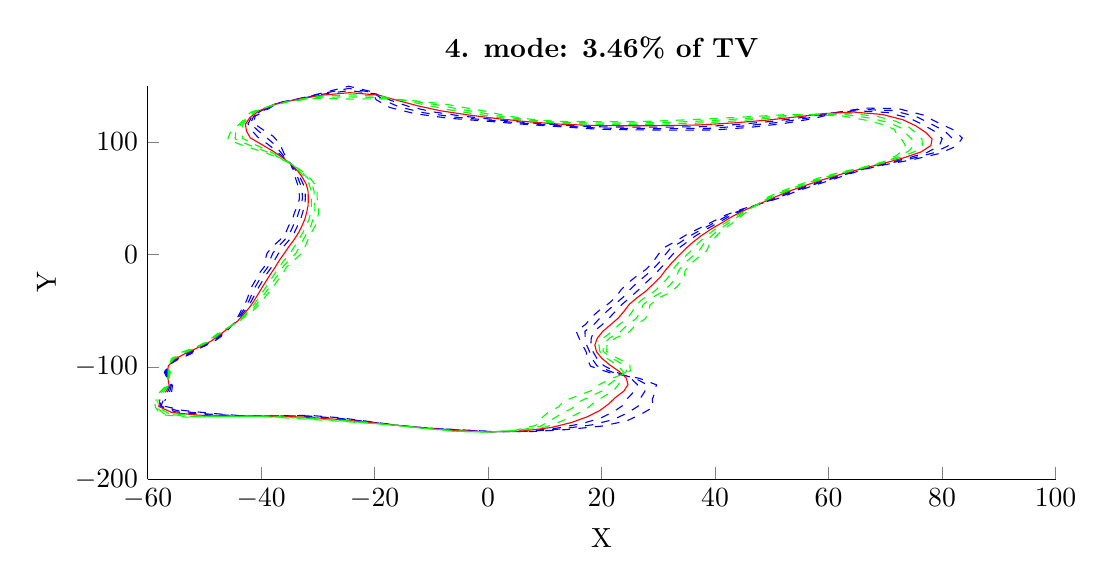
\begin{tikzpicture}

\begin{axis}[%
width=0.95092\figurewidth,
height=\figureheight,
at={(0\figurewidth,0\figureheight)},
scale only axis,
xmin=-60,
xmax=100,
xlabel={X},
ymin=-200,
ymax=150,
ylabel={Y},
title style={font=\bfseries},
title={4. mode: 3.46\% of TV},
axis x line*=bottom,
axis y line*=left
]
\addplot [color=blue,dashed,forget plot]
  table[row sep=crcr]{%
-55.7671478581589	-122.321913351108\\
-55.6278150195823	-116.615739101658\\
-56.4477919720177	-110.880391236616\\
-57.0461645834889	-105.120570922306\\
-56.5853228149416	-99.3743655577022\\
-54.832584111751	-93.9927788599231\\
-52.4661006595763	-88.7443004097182\\
-50.6893162582924	-83.2505413024613\\
-48.3774989466764	-77.7828915707806\\
-46.6931196289506	-71.8441556526405\\
-45.605738901637	-65.7493571159346\\
-44.5354818916976	-59.6601074623189\\
-43.8672509860657	-53.5001806373197\\
-43.2648489721604	-47.3308200598009\\
-42.5648492892032	-41.2009528131994\\
-42.1307802409872	-35.0533160405411\\
-41.6714763935451	-28.9639855906577\\
-40.980538970988	-22.9518346354312\\
-40.3402798419909	-16.9558921546429\\
-39.4219890972119	-10.9811073811457\\
-39.2819784302045	-4.91196512796911\\
-38.9395600952014	1.08454038162261\\
-37.9365998071035	7.05691172428768\\
-36.646628064849	12.9537994820837\\
-35.6667351769732	18.9950998719473\\
-35.1523585702267	25.1825776910809\\
-34.4715296301277	31.3656585935823\\
-34.077809652189	37.5608383136098\\
-33.4825891773774	43.7484428439088\\
-33.2400887883156	49.9550671492517\\
-33.2953518929503	56.1538896409896\\
-33.5874773215985	62.3489179707207\\
-33.9867609383386	68.4827678744262\\
-34.3465211139525	74.5733909849328\\
-34.8444815256729	80.6571135952166\\
-35.69442475793	86.7144585131018\\
-36.2380226855839	92.8536753162924\\
-36.7860815107187	98.979266011445\\
-37.8903248787309	104.998291519216\\
-39.7177414394695	110.894220210656\\
-41.400232477308	116.760175793093\\
-41.0301204912834	122.833635905796\\
-38.9227198826552	128.650621006345\\
-37.0882695894333	134.647879754848\\
-32.7465312707264	139.035493726877\\
-28.6227205799706	144.142270561673\\
-24.5763128446133	149.413540068921\\
-20.5600641895921	144.640390227893\\
-19.7186717492652	137.390274725925\\
-17.3119663734036	130.492807895694\\
-12.8701555370302	124.991711605079\\
-6.99247805181616	120.966213464162\\
-0.253287557602013	118.365342023111\\
6.25106949709879	115.632304960374\\
12.8966178362376	113.378181745622\\
19.6247350728654	111.10268314654\\
26.4556439098168	110.606186861246\\
33.0722310810186	110.407465367564\\
39.7579251615119	110.478221352818\\
46.0636322547803	112.806698412262\\
51.9255388907054	116.132741041483\\
57.2240059074804	120.53627513553\\
61.5481585556242	126.023102010047\\
66.2177425297651	129.996319050366\\
72.2685641761597	129.480880331779\\
76.6358252140077	123.876604021438\\
79.2407256425268	117.080778371209\\
82.1261164019117	110.376468634383\\
83.5710655984914	103.329036926173\\
82.5635426518981	96.1809922449125\\
79.4702666211068	89.5263453126273\\
74.6621940792365	83.9464653644022\\
69.8060481902468	79.5127652387231\\
66.0408405353527	75.2112485894343\\
63.0052265831773	70.3094975229699\\
60.0165446900388	65.3738923162652\\
56.9750163012031	60.4558971017298\\
54.0492631729989	55.4800291103163\\
51.5535202671159	50.300488404952\\
48.3319817462601	45.4526400863397\\
44.9018990922493	40.4252413887496\\
41.863133369803	34.8483239083195\\
39.5452265128931	28.9960778441368\\
37.2518412500286	23.1619167426311\\
34.9386138851473	17.3014807642325\\
32.9686852489067	11.3316103660564\\
30.8078108566926	5.39652786063002\\
29.9051654572101	-0.809483617677981\\
29.0306368620779	-7.05532130958782\\
27.8731819122272	-13.2361148847907\\
26.1913755388832	-19.3170079880804\\
24.6756052757016	-25.4398454243971\\
23.4193606376008	-31.6148170712085\\
22.58388428785	-37.7834613590749\\
21.2308355754016	-43.8551093091569\\
19.5758556107709	-49.9372823095955\\
18.197968506294	-56.0701397471498\\
17.2038782221054	-62.2779790398612\\
15.5120566579522	-68.2614395088515\\
16.0380911482394	-74.5747211749134\\
16.6758422318416	-80.8929236011453\\
17.315572040998	-87.0598721625458\\
17.4828738419463	-93.1945522858675\\
18.0512687213708	-99.4509730122356\\
21.3145854487483	-105.089642641894\\
26.671690847947	-110.286297737295\\
29.6632982105476	-116.013021644582\\
29.4167097570331	-122.40448204076\\
28.9390147167332	-129.07110336665\\
29.0604565628521	-136.005354643069\\
26.9656918188967	-142.132870134174\\
24.4529889219434	-148.070616107286\\
20.049328386216	-152.749896313743\\
13.7712049822315	-155.870958510231\\
7.61740337308566	-157.613497490227\\
1.40485592192719	-157.626739270639\\
-4.71759986924361	-156.075391163665\\
-10.5467903138167	-154.475223796544\\
-16.0431049161759	-151.944169746529\\
-21.070254969413	-148.562964561615\\
-26.119409156266	-145.313694780192\\
-31.506634400997	-143.20017846602\\
-37.4817972173019	-143.70780723422\\
-43.3280281274039	-143.562292868944\\
-48.7917471045956	-141.395492305958\\
-53.7551542947874	-138.800527635889\\
-57.4456246874674	-134.590110465091\\
-56.8258990376135	-128.764521293749\\
};
\addplot [color=blue,dashed,forget plot]
  table[row sep=crcr]{%
-56.1331269243892	-122.456282688173\\
-55.8212199741377	-116.722521346848\\
-56.4291406725886	-110.928442260132\\
-56.8720010594027	-105.11896609606\\
-56.5054098939443	-99.3279094853385\\
-54.9998910107335	-93.8167525337546\\
-52.7349396439063	-88.4845939658886\\
-50.7759163623979	-83.0213567804053\\
-48.5068099928875	-77.5326887931878\\
-46.8617404988902	-71.6241151267789\\
-45.6269381315741	-65.6052765810274\\
-44.4115057645962	-59.5914707998421\\
-43.6142337426461	-53.4933849410745\\
-42.8728623100303	-47.3860825879397\\
-42.1296453801045	-41.2963504863352\\
-41.5991652492173	-35.1887490811743\\
-41.0515941634283	-29.118005760099\\
-40.3432059900465	-23.0942199963864\\
-39.6591986637268	-17.0827499574596\\
-38.779705499666	-11.0853687761439\\
-38.4438294638689	-5.00152479781899\\
-37.9313155732565	1.00462602832451\\
-36.9890035497878	6.99967682951489\\
-35.8300269161488	12.9394826861861\\
-34.9189092576625	18.9977193926211\\
-34.3712403688829	25.174369094033\\
-33.742568658564	31.3518006259345\\
-33.3707586776167	37.5414293533254\\
-32.8913889389768	43.7257679916075\\
-32.7220472507548	49.9243315231374\\
-32.7683855098103	56.1152946734957\\
-33.0726926294788	62.3023775255535\\
-33.563742080303	68.4250088325555\\
-34.0915332580827	74.495946264532\\
-34.8087621799512	80.5516581595761\\
-35.8995310869488	86.5581256638336\\
-36.8386099342084	92.5965625344409\\
-37.8462067507139	98.584363652231\\
-39.2266279947445	104.49877218486\\
-40.6695006355496	110.431570594539\\
-41.8571733012318	116.345398007976\\
-41.3521560823237	122.399911265136\\
-39.4167578983966	128.24274599043\\
-37.3517464329917	134.085526433012\\
-33.1087882101996	138.53261503411\\
-28.8535128533538	143.24362386752\\
-24.5001051059426	147.508866204685\\
-20.1365145114408	143.586037841544\\
-18.4574460880736	137.171313056681\\
-15.6728604783291	130.986984409536\\
-11.3575672523661	125.840161542988\\
-5.83984847610367	121.943223839331\\
0.337768928221238	119.135386343509\\
6.44023389070865	116.388040873473\\
12.7409519794786	114.172727141124\\
19.1868027665596	112.254142541565\\
25.802970375666	111.819449557307\\
32.3548722445234	111.719548982603\\
38.9224214952653	111.980315256824\\
45.1536688837614	114.15037737895\\
51.0161874930084	117.184968811417\\
56.3598782247902	121.120929232606\\
60.7876641717961	125.713140895753\\
65.6028510626145	128.81872719464\\
71.3384066669887	127.75233141794\\
75.4506510250658	122.462110389408\\
77.9620326740962	116.10253813876\\
80.4495016212243	109.728566834892\\
81.7967843343668	103.085421749959\\
81.0553175697596	96.3441137467711\\
78.4098082085978	90.0129473947556\\
74.2098364813492	84.5802020174303\\
69.8082191385499	80.0110563787474\\
66.0547701369136	75.5763463888988\\
62.8207351400986	70.7175316331518\\
59.7171245351805	65.7565964804096\\
56.651354912472	60.756516530664\\
53.7114897470232	55.688472114804\\
51.1871383733549	50.4196884071692\\
48.2113034966755	45.357772710729\\
45.0638182683564	40.165260351376\\
42.2812664899028	34.5366789166978\\
40.1020461084169	28.6784308978903\\
37.9160131576293	22.845879879202\\
35.7926070306529	16.971013587484\\
33.9813927900136	10.998328317768\\
32.0976975339318	5.03561304850041\\
31.1017727099116	-1.11145131724627\\
30.1334582327009	-7.31128454732046\\
29.0134234362619	-13.4924139576903\\
27.581649197117	-19.6093578135868\\
26.163426430386	-25.7378328405225\\
24.9060696646854	-31.8906374410735\\
23.8236412645173	-37.9995529035271\\
22.4450013306196	-44.066338829105\\
21.0391407794442	-50.168670758335\\
19.7786736643828	-56.2847449882645\\
18.6616423174864	-62.4097288266055\\
17.0762546407774	-68.3728826941567\\
17.1101324896126	-74.5557203578896\\
17.3904913592265	-80.7878913703157\\
17.9123859977023	-86.9380843379607\\
18.3497004011108	-93.026333218887\\
19.2050741563943	-99.1684067445433\\
21.9393391618771	-104.867158967887\\
25.8992786242202	-110.220479924635\\
27.9945493508259	-115.94631442914\\
27.5936703864811	-122.109043404952\\
26.7762804548439	-128.481170925551\\
26.4488381981572	-135.045405546958\\
24.5372706234196	-141.057578044772\\
22.1254551236025	-146.875964617701\\
18.2469454886421	-151.703106738459\\
12.8715801010257	-155.261888352872\\
7.12011706400886	-157.424576097233\\
1.07446584961165	-157.706685956514\\
-4.90033854788316	-156.313191146289\\
-10.6206084569935	-154.54982265961\\
-16.0503547953732	-151.97872853533\\
-21.1413885955493	-148.809187561863\\
-26.3311361610854	-145.758615559609\\
-31.8825610674558	-143.674635055751\\
-37.9194662904745	-143.780054705394\\
-43.8929542316296	-143.656445426162\\
-49.5025702052924	-141.956967506543\\
-54.4244102013612	-139.403189020094\\
-57.6392690082732	-134.833029219973\\
-57.1627539103238	-128.824844974409\\
};
\addplot [color=blue,dashed,forget plot]
  table[row sep=crcr]{%
-56.4991059906196	-122.590652025239\\
-56.0146249286931	-116.829303592038\\
-56.4104893731595	-110.976493283648\\
-56.6978375353166	-105.117361269815\\
-56.425496972947	-99.2814534129748\\
-55.1671979097159	-93.640726207586\\
-53.0037786282363	-88.2248875220591\\
-50.8625164665034	-82.7921722583493\\
-48.6361210390986	-77.282486015595\\
-47.0303613688299	-71.4040746009174\\
-45.6481373615111	-65.4611960461202\\
-44.2875296374948	-59.5228341373652\\
-43.3612164992266	-53.4865892448292\\
-42.4808756479002	-47.4413451160785\\
-41.6944414710058	-41.3917481594709\\
-41.0675502574473	-35.3241821218075\\
-40.4317119333116	-29.2720259295403\\
-39.7058730091049	-23.2366053573415\\
-38.9781174854627	-17.2096077602762\\
-38.1374219021201	-11.1896301711421\\
-37.6056804975333	-5.09108446766887\\
-36.9230710513115	0.924711675026402\\
-36.041407292472	6.9424419347421\\
-35.0134257674485	12.9251658902885\\
-34.1710833383519	19.0003389132949\\
-33.5901221675391	25.1661604969851\\
-33.0136076870003	31.3379426582867\\
-32.6637077030443	37.5220203930411\\
-32.3001887005762	43.7030931393061\\
-32.2040057131939	49.8935958970232\\
-32.2414191266703	56.0766997060018\\
-32.557907937359	62.2558370803863\\
-33.1407232222673	68.3672497906848\\
-33.8365454022129	74.4185015441312\\
-34.7730428342296	80.4462027239357\\
-36.1046374159676	86.4017928145654\\
-37.439197182833	92.3394497525895\\
-38.906331990709	98.189461293017\\
-40.5629311107581	103.999252850504\\
-41.6212598316298	109.968920978422\\
-42.3141141251555	115.93062022286\\
-41.674191673364	121.966186624477\\
-39.910795914138	127.834870974516\\
-37.6152232765501	133.523173111177\\
-33.4710451496729	138.029736341344\\
-29.0843051267371	142.344977173366\\
-24.4238973672718	145.60419234045\\
-19.7129648332896	142.531685455196\\
-17.196220426882	136.952351387436\\
-14.0337545832546	131.481160923379\\
-9.84497896770199	126.688611480897\\
-4.68721890039118	122.9202342145\\
0.928825414044488	119.905430663907\\
6.62939828431852	117.143776786573\\
12.5852861227197	114.967272536626\\
18.7488704602539	113.405601936589\\
25.1502968415151	113.032712253367\\
31.6375134080283	113.031632597642\\
38.0869178290187	113.48240916083\\
44.2437055127425	115.494056345638\\
50.1068360953114	118.23719658135\\
55.4957505421001	121.705583329682\\
60.027169787968	125.40317978146\\
64.9879595954639	127.641135338915\\
70.4082491578177	126.023782504101\\
74.2654768361239	121.047616757378\\
76.6833397056656	115.124297906312\\
78.7728868405368	109.080665035401\\
80.0225030702421	102.841806573745\\
79.5470924876212	96.5072352486297\\
77.3493497960888	90.4995494768839\\
73.757478883462	85.2139386704583\\
69.8103900868531	80.5093475187717\\
66.0686997384746	75.9414441883633\\
62.6362436970199	71.1255657433337\\
59.4177043803222	66.139300644554\\
56.3276935237409	61.0571359595982\\
53.3737163210475	55.8969151192916\\
50.8207564795939	50.5388884093865\\
48.0906252470909	45.2629053351183\\
45.2257374444635	39.9052793140024\\
42.6993996100027	34.225033925076\\
40.6588657039408	28.3607839516438\\
38.58018506523	22.5298430157729\\
36.6466001761584	16.6405464107355\\
34.9941003311204	10.6650462694797\\
33.3875842111711	4.67469823637081\\
32.2983799626131	-1.41341901681456\\
31.2362796033238	-7.5672477850531\\
30.1536649602967	-13.7487130305899\\
28.9719228553509	-19.9017076390932\\
27.6512475850704	-26.0358202566478\\
26.39277869177	-32.1664578109385\\
25.0633982411846	-38.2156444479794\\
23.6591670858377	-44.2775683490531\\
22.5024259481175	-50.4000592070745\\
21.3593788224715	-56.4993502293792\\
20.1194064128674	-62.5414786133499\\
18.6404526236026	-68.4843258794618\\
18.1821738309857	-74.5367195408659\\
18.1051404866114	-80.6828591394861\\
18.5091999544067	-86.8162965133756\\
19.2165269602752	-92.8581141519065\\
20.3588795914178	-98.885840476851\\
22.564092875006	-104.64467529388\\
25.1268664004934	-110.154662111976\\
26.3258004911042	-115.879607213698\\
25.7706310159291	-121.813604769144\\
24.6135461929545	-127.891238484452\\
23.8372198334623	-134.085456450847\\
22.1088494279425	-139.982285955369\\
19.7979213252617	-145.681313128117\\
16.4445625910683	-150.656317163175\\
11.97195521982	-154.652818195514\\
6.62283075493207	-157.235654704239\\
0.744075777296116	-157.786632642389\\
-5.08307722652271	-156.550991128913\\
-10.6944266001703	-154.624421522676\\
-16.0576046745704	-152.013287324131\\
-21.2125222216856	-149.055410562112\\
-26.5428631659047	-146.203536339026\\
-32.2584877339145	-144.149091645481\\
-38.3571353636472	-143.852302176567\\
-44.4578803358553	-143.75059798338\\
-50.2133933059892	-142.518442707129\\
-55.0936661079351	-140.005850404299\\
-57.8329133290791	-135.075947974855\\
-57.499608783034	-128.885168655068\\
};
\addplot [color=red,solid,forget plot]
  table[row sep=crcr]{%
-56.8650850568499	-122.725021362305\\
-56.2080298832485	-116.936085837228\\
-56.3918380737305	-111.024544307164\\
-56.5236740112305	-105.115756443569\\
-56.3455840519496	-99.234997340611\\
-55.3345048086984	-93.4646998814174\\
-53.2726176125663	-87.9651810782296\\
-50.949116570609	-82.5629877362933\\
-48.7654320853097	-77.0322832380022\\
-47.1989822387695	-71.1840340750558\\
-45.6693365914481	-65.317115511213\\
-44.1635535103934	-59.4541974748884\\
-43.1081992558071	-53.479793548584\\
-42.0888889857701	-47.4966076442174\\
-41.2592375619071	-41.4871458326067\\
-40.5359352656773	-35.4596151624407\\
-39.8118297031948	-29.4260460989816\\
-39.0685400281634	-23.3789907182966\\
-38.2970363071987	-17.3364655630929\\
-37.4951383045741	-11.2938915661403\\
-36.7675315311977	-5.18064413751875\\
-35.9148265293666	0.844797321728298\\
-35.0938110351563	6.88520703996931\\
-34.1968246187483	12.9108490943909\\
-33.4232574190412	19.0029584339687\\
-32.8090039661952	25.1579518999372\\
-32.2846467154367	31.324084690639\\
-31.956656728472	37.5026114327567\\
-31.7089884621756	43.6804182870047\\
-31.685964175633	49.8628602709089\\
-31.7144527435303	56.038104738508\\
-32.0431232452393	62.209296635219\\
-32.7177043642317	68.3094907488142\\
-33.5815575463431	74.3410568237305\\
-34.737323488508	80.3407472882952\\
-36.3097437449864	86.2454599652972\\
-38.0397844314575	92.082336970738\\
-39.9664572307042	97.794558933803\\
-41.8992342267718	103.499733516148\\
-42.57301902771	109.506271362305\\
-42.7710549490792	115.515842437744\\
-41.9962272644043	121.532461983817\\
-40.4048339298793	127.426995958601\\
-37.8787001201085	132.960819789342\\
-33.8333020891462	137.526857648577\\
-29.3150974001203	141.446330479213\\
-24.3476896286011	143.699518476214\\
-19.2894151551383	141.477333068848\\
-15.9349947656904	136.733389718192\\
-12.3946486881801	131.975337437221\\
-8.33239068303789	127.537061418806\\
-3.53458932467869	123.897244589669\\
1.51988189986774	120.675474984305\\
6.81856267792838	117.899512699672\\
12.4296202659607	115.761817932129\\
18.3109381539481	114.557061331613\\
24.4976233073643	114.245974949428\\
30.9201545715332	114.343716212681\\
37.251414162772	114.984503064837\\
43.3337421417236	116.837735312326\\
49.1974846976144	119.289424351283\\
54.6316228594099	122.290237426758\\
59.2666754041399	125.093218667167\\
64.3730681283133	126.463543483189\\
69.4780916486468	124.295233590262\\
73.0803026471819	119.633123125349\\
75.4046467372349	114.146057673863\\
77.0962720598493	108.43276323591\\
78.2482218061175	102.598191397531\\
78.0388674054827	96.6703567504883\\
76.2888913835798	90.9861515590123\\
73.3051212855748	85.8476753234863\\
69.8125610351563	81.007638658796\\
66.0826293400356	76.3065419878278\\
62.4517522539411	71.5335998535156\\
59.1182842254639	66.5220048086984\\
56.0040321350098	61.3577553885324\\
53.0359428950718	56.1053581237793\\
50.4543745858329	50.6580884116037\\
47.9699469975063	45.1680379595075\\
45.3876566205706	39.6452982766288\\
43.1175327301025	33.9133889334542\\
41.2156852994646	28.0431370053973\\
39.2443569728306	22.2138061523438\\
37.500593321664	16.310079233987\\
36.0068078722273	10.3317642211914\\
34.6774708884103	4.3137834242412\\
33.4949872153146	-1.71538671638284\\
32.3391009739467	-7.82321102278573\\
31.2939064843314	-14.0050121034895\\
30.3621965135847	-20.1940574645996\\
29.1390687397548	-26.3338076727731\\
27.8794877188546	-32.4422781808036\\
26.3031552178519	-38.4317359924316\\
24.8733328410557	-44.4887978690011\\
23.9657111167908	-50.631447655814\\
22.9400839805603	-56.7139554704939\\
21.5771705082485	-62.6732284000942\\
20.2046506064279	-68.595769064767\\
19.2542151723589	-74.5177187238421\\
18.8197896139962	-80.5778269086565\\
19.106013911111	-86.6945086887905\\
20.0833535194397	-92.6898950849261\\
21.5126850264413	-98.6032742091588\\
23.1888465881348	-104.422191619873\\
24.3544541767665	-110.088844299316\\
24.6570516313825	-115.812899998256\\
23.947591645377	-121.518166133336\\
22.4508119310652	-127.301306043352\\
21.2256014687674	-133.125507354736\\
19.6804282324655	-138.906993865967\\
17.4703875269209	-144.486661638532\\
14.6421796934945	-149.609527587891\\
11.0723303386143	-154.043748038156\\
6.12554444585528	-157.046733311244\\
0.413685704980578	-157.866579328265\\
-5.26581590516227	-156.788791111537\\
-10.7682447433472	-154.699020385742\\
-16.0648545537676	-152.047846112932\\
-21.2836558478219	-149.30163356236\\
-26.7545901707241	-146.648457118443\\
-32.6344144003732	-144.623548235212\\
-38.7948044368199	-143.92454964774\\
-45.0228064400809	-143.844750540597\\
-50.924216406686	-143.079917907715\\
-55.7629220145089	-140.608511788504\\
-58.0265576498849	-135.318866729736\\
-57.8364636557443	-128.945492335728\\
};
\addplot [color=green,dashed,forget plot]
  table[row sep=crcr]{%
-57.2310641230802	-122.85939069937\\
-56.4014348378039	-117.042868082418\\
-56.3731867743014	-111.07259533068\\
-56.3495104871443	-105.114151617323\\
-56.2656711309523	-99.1885412682473\\
-55.5018117076809	-93.2886735552488\\
-53.5414565968962	-87.7054746344001\\
-51.0357166747145	-82.3338032142372\\
-48.8947431315208	-76.7820804604095\\
-47.3676031087092	-70.9639935491942\\
-45.6905358213851	-65.1730349763058\\
-44.039577383292	-59.3855608124116\\
-42.8551820123875	-53.4729978523388\\
-41.69690232364	-47.5518701723562\\
-40.8240336528084	-41.5825435057425\\
-40.0043202739073	-35.5950482030739\\
-39.191947473078	-29.5800662684229\\
-38.4312070472218	-23.5213760792517\\
-37.6159551289346	-17.4633233659096\\
-36.8528547070282	-11.3981529611385\\
-35.9293825648621	-5.27020380736862\\
-34.9065820074217	0.764882968430194\\
-34.1462147778405	6.82797214519652\\
-33.380223470048	12.8965322984932\\
-32.6754314997306	19.0055779546425\\
-32.0278857648514	25.1497433028893\\
-31.555685743873	31.3102267229912\\
-31.2496057538997	37.4832024724723\\
-31.117788223775	43.6577434347034\\
-31.1679226380722	49.8321246447946\\
-31.1874863603903	55.9995097710141\\
-31.5283385531195	62.1627561900518\\
-32.294685506196	68.2517317069435\\
-33.3265696904733	74.2636121033297\\
-34.7016041427863	80.2352918526547\\
-36.5148500740052	86.0891271160289\\
-38.6403716800821	91.8252241888865\\
-41.0265824706993	97.399656574589\\
-43.2355373427854	103.000214181792\\
-43.5247782237901	109.043621746188\\
-43.227995773003	115.101064652628\\
-42.3182628554446	121.098737343157\\
-40.8988719456207	127.019120942686\\
-38.1421769636669	132.398466467506\\
-34.1955590286195	137.02397895581\\
-29.5458896735036	140.54768378506\\
-24.2714818899303	141.794844611978\\
-18.865865476987	140.422980682499\\
-14.6737691044988	136.514428048947\\
-10.7555427931056	132.469513951063\\
-6.8198023983738	128.385511356715\\
-2.3819597489662	124.874254964839\\
2.11093838569099	121.445519304703\\
7.00772707153824	118.655248612772\\
12.2739544092017	116.556363327631\\
17.8730058476424	115.708520726637\\
23.8449497732135	115.459237645489\\
30.2027957350381	115.655799827721\\
36.4159104965254	116.486596968843\\
42.4237787707047	118.181414279013\\
48.2881332999174	120.341652121217\\
53.7674951767197	122.874891523834\\
58.5061810203118	124.783257552873\\
63.7581766611628	125.285951627464\\
68.5479341394758	122.566684676423\\
71.89512845824	118.218629493319\\
74.1259537688043	113.167817441414\\
75.4196572791619	107.784861436418\\
76.4739405419928	102.354576221317\\
76.5306423233442	96.8334782523469\\
75.2284329710708	91.4727536411406\\
72.8527636876875	86.4814119765144\\
69.8147319834594	81.5059297988203\\
66.0965589415966	76.6716397872923\\
62.2672608108624	71.9416339636975\\
58.8188640706056	66.9047089728428\\
55.6803707462786	61.6583748174665\\
52.6981694690962	56.313801128267\\
50.0879926920719	50.7772884138209\\
47.8492687479217	45.0731705838968\\
45.5495757966777	39.3853172392551\\
43.5356658502024	33.6017439418325\\
41.7725048949885	27.7254900591507\\
39.9085288804313	21.8977692889146\\
38.3545864671696	15.9796120572385\\
37.0195154133341	9.99848217290309\\
35.9673575656495	3.9528686121116\\
34.6915944680161	-2.01735441595113\\
33.4419223445696	-8.07917426051837\\
32.4341480083661	-14.261311176389\\
31.7524701718185	-20.486407290106\\
30.6268898944392	-26.6317950888984\\
29.3661967459392	-32.7180985506686\\
27.5429121945192	-38.6478275368839\\
26.0874985962738	-44.7000273889492\\
25.4289962854641	-50.8628361045535\\
24.5207891386491	-56.9285607116086\\
23.0349346036295	-62.8049781868385\\
21.7688485892531	-68.7072122500722\\
20.3262565137321	-74.4987179068183\\
19.5344387413811	-80.4727946778269\\
19.7028278678153	-86.5727208642053\\
20.9501800786042	-92.5216760179456\\
22.6664904614648	-98.3207079414665\\
23.8136003012636	-104.199707945866\\
23.5820419530397	-110.023026486657\\
22.9883027716609	-115.746192782814\\
22.124552274825	-121.222727497527\\
20.2880776691758	-126.711373602253\\
18.6139831040725	-132.165558258626\\
17.2520070369884	-137.831701776564\\
15.14285372858	-143.292010148948\\
12.8397967959207	-148.562738012606\\
10.1727054574086	-153.434677880797\\
5.62825813677848	-156.85781191825\\
0.0832956326650399	-157.94652601414\\
-5.44855458380182	-157.026591094162\\
-10.842062886524	-154.773619248808\\
-16.0721044329648	-152.082404901734\\
-21.3547894739582	-149.547856562609\\
-26.9663171755434	-147.09337789786\\
-33.0103410668319	-145.098004824943\\
-39.2324735099926	-143.996797118913\\
-45.5877325443066	-143.938903097815\\
-51.6350395073827	-143.641393108301\\
-56.4321779210828	-141.21117317271\\
-58.2202019706907	-135.561785484618\\
-58.1733185284545	-129.005816016388\\
};
\addplot [color=green,dashed,forget plot]
  table[row sep=crcr]{%
-57.5970431893105	-122.993760036436\\
-56.5948397923593	-117.149650327608\\
-56.3545354748723	-111.120646354195\\
-56.1753469630582	-105.112546791077\\
-56.185758209955	-99.1420851958836\\
-55.6691186066633	-93.1126472290803\\
-53.8102955812262	-87.4457681905706\\
-51.12231677882	-82.1046186921812\\
-49.0240541777319	-76.5318776828167\\
-47.5362239786488	-70.7439530233327\\
-45.7117350513222	-65.0289544413986\\
-43.9156012561906	-59.3169241499347\\
-42.602164768968	-53.4662021560935\\
-41.3049156615099	-47.607132700495\\
-40.3888297437097	-41.6779411788783\\
-39.4727052821374	-35.7304812437071\\
-38.5720652429612	-29.7340864378642\\
-37.7938740662803	-23.6637614402068\\
-36.9348739506705	-17.5901811687262\\
-36.2105711094823	-11.5024143561367\\
-35.0912335985265	-5.3597634772185\\
-33.8983374854768	0.68496861513209\\
-33.1986185205247	6.77073725042373\\
-32.5636223213478	12.8822155025956\\
-31.9276055804199	19.0081974753163\\
-31.2467675635076	25.1415347058415\\
-30.8267247723093	31.2963687553434\\
-30.5425547793274	37.463793512188\\
-30.5265879853745	43.635068582402\\
-30.6498811005113	49.8013890186804\\
-30.6605199772503	55.9609148035202\\
-31.0135538609997	62.1162157448846\\
-31.8716666481603	68.1939726650728\\
-33.0715818346035	74.1861673829289\\
-34.6658847970647	80.1298364170143\\
-36.719956403024	85.9327942667607\\
-39.2409589287066	91.5681114070351\\
-42.0867077106945	97.004754215375\\
-44.571840458799	102.500694847436\\
-44.4765374198703	108.580972130071\\
-43.6849365969267	114.686286867512\\
-42.6402984464849	120.665012702497\\
-41.3929099613621	126.611245926771\\
-38.4056538072253	131.836113145671\\
-34.5578159680928	136.521100263044\\
-29.7766819468868	139.649037090907\\
-24.1952741512596	139.890170747742\\
-18.4423157988358	139.368628296151\\
-13.4125434433072	136.295466379703\\
-9.11643689803112	132.963690464906\\
-5.3072141137097	129.233961294624\\
-1.22933017325371	125.851265340008\\
2.70199487151424	122.215563625102\\
7.19689146514811	119.410984525871\\
12.1182885524427	117.350908723134\\
17.4350735413366	116.859980121661\\
23.1922762390627	116.672500341549\\
29.485436898543	116.96788344276\\
35.5804068302788	117.98869087285\\
41.5138153996859	119.525093245701\\
47.3787819022204	121.39387989115\\
52.9033674940295	123.459545620909\\
57.7456866364837	124.47329643858\\
63.1432851940122	124.108359771738\\
67.6177766303048	120.838135762584\\
70.7099542692981	116.80413586129\\
72.8472608003736	112.189577208966\\
73.7430424984744	107.136959636927\\
74.6996592778682	102.110961045103\\
75.0224172412058	96.9965997542055\\
74.1679745585618	91.9593557232689\\
72.4004060898003	87.1151486295424\\
69.8169029317626	82.0042209388447\\
66.1104885431575	77.0367375867569\\
62.0827693677837	72.3496680738795\\
58.5194439157472	67.2874131369872\\
55.3567093575475	61.9589942464007\\
52.3603960431205	56.5222441327546\\
49.7216107983109	50.8964884160381\\
47.7285904983371	44.9783032082861\\
45.7114949727848	39.1253362018815\\
43.9537989703022	33.2900989502107\\
42.3293244905123	27.4078431129042\\
40.572700788032	21.5817324254855\\
39.2085796126751	15.64914488049\\
38.032222954441	9.66520012461477\\
37.2572442428888	3.59195379998199\\
35.8882017207176	-2.31932211551942\\
34.5447437151925	-8.335137498251\\
33.5743895324009	-14.5176102492886\\
33.1427438300523	-20.7787571156124\\
32.1147110491236	-26.9297825050237\\
30.8529057730238	-32.9939189205336\\
28.7826691711865	-38.8639190813361\\
27.3016643514918	-44.9112569088972\\
26.8922814541374	-51.0942245532931\\
26.1014942967378	-57.1431659527233\\
24.4926986990105	-62.9367279735828\\
23.3330465720783	-68.8186554353774\\
21.3982978551053	-74.4797170897945\\
20.249087868766	-80.3677624469973\\
20.2996418245197	-86.4509330396202\\
21.8170066377686	-92.3534569509651\\
23.8202958964883	-98.0381416737742\\
24.4383540143924	-103.977224271859\\
22.8096297293129	-109.957208673998\\
21.3195539119392	-115.679485567372\\
20.301512904273	-120.927288861719\\
18.1253434072864	-126.121441161154\\
16.0023647393777	-131.205609162515\\
14.8235858415113	-136.756409687162\\
12.8153199302392	-142.097358659363\\
11.0374138983469	-147.515948437322\\
9.27308057620291	-152.825607723439\\
5.13097182770169	-156.668890525256\\
-0.247094439650498	-158.026472700015\\
-5.63129326244137	-157.264391076786\\
-10.9158810297008	-154.848218111874\\
-16.0793543121621	-152.116963690535\\
-21.4259231000946	-149.794079562858\\
-27.1780441803627	-147.538298677277\\
-33.3862677332906	-145.572461414674\\
-39.6701425831653	-144.069044590086\\
-46.1526586485322	-144.033055655032\\
-52.3458626080795	-144.202868308886\\
-57.1014338276566	-141.813834556915\\
-58.4138462914966	-135.8047042395\\
-58.5101734011648	-129.066139697048\\
};
\addplot [color=green,dashed,forget plot]
  table[row sep=crcr]{%
-57.9630222555409	-123.128129373502\\
-56.7882447469147	-117.256432572798\\
-56.3358841754433	-111.168697377711\\
-56.001183438972	-105.110941964831\\
-56.1058452889576	-99.0956291235199\\
-55.8364255056458	-92.9366209029117\\
-54.0791345655562	-87.1860617467411\\
-51.2089168829255	-81.8754341701252\\
-49.153365223943	-76.2816749052239\\
-47.7048448485885	-70.5239124974711\\
-45.7329342812592	-64.8848739064914\\
-43.7916251290892	-59.2482874874579\\
-42.3491475255484	-53.4594064598483\\
-40.9129289993798	-47.6623952286338\\
-39.953625834611	-41.7733388520141\\
-38.9410902903674	-35.8659142843403\\
-37.9521830128444	-29.8881066073055\\
-37.1565410853387	-23.806146801162\\
-36.2537927724064	-17.7170389715429\\
-35.5682875119364	-11.6066757511349\\
-34.2530846321908	-5.44932314706838\\
-32.8900929635319	0.605054261833985\\
-32.251022263209	6.71350235565094\\
-31.7470211726475	12.867898706698\\
-31.1797796611093	19.0108169959901\\
-30.4656493621638	25.1333261087936\\
-30.0977638007456	31.2825107876956\\
-29.8355038047551	37.4443845519036\\
-29.9353877469739	43.6123937301007\\
-30.1318395629504	49.7706533925661\\
-30.1335535941103	55.9223198360263\\
-30.49876916888	62.0696752997173\\
-31.4486477901247	68.1362136232022\\
-32.8165939787337	74.1087226625281\\
-34.630165451343	80.0243809813738\\
-36.9250627320428	85.7764614174925\\
-39.8415461773311	91.3109986251836\\
-43.1468329506896	96.609851856161\\
-45.9081435748126	102.00117551308\\
-45.4282966159505	108.118322513954\\
-44.1418774208505	114.271509082396\\
-42.9623340375252	120.231288061838\\
-41.8869479771034	126.203370910856\\
-38.6691306507837	131.273759823835\\
-34.9200729075661	136.018221570277\\
-30.0074742202701	138.750390396753\\
-24.1190664125888	137.985496883506\\
-18.0187661206845	138.314275909803\\
-12.1513177821156	136.076504710459\\
-7.47733100295663	133.457866978748\\
-3.7946258290456	130.082411232533\\
-0.0767005975412229	126.828275715177\\
3.29305135733749	122.9856079455\\
7.38605585875797	120.16672043897\\
11.9626226956838	118.145454118636\\
16.9971412350308	118.011439516685\\
22.5396027049119	117.88576303761\\
28.7680780620479	118.279967057799\\
34.7449031640322	119.490784776856\\
40.603852028667	120.868772212389\\
46.4694305045234	122.446107661084\\
52.0392398113393	124.044199717985\\
56.9851922526556	124.163335324286\\
62.5283937268616	122.930767916013\\
66.6876191211338	119.109586848746\\
69.5247800803562	115.38964222926\\
71.568567831943	111.211336976517\\
72.0664277177869	106.489057837436\\
72.9253780137435	101.867345868889\\
73.5141921590673	97.1597212560641\\
73.1075161460528	92.4459578053972\\
71.9480484919131	87.7488852825704\\
69.8190738800657	82.502512078869\\
66.1244181447185	77.4018353862214\\
61.8982779247049	72.7577021840614\\
58.2200237608889	67.6701173011316\\
55.0330479688164	62.2596136753349\\
52.0226226171448	56.7306871372423\\
49.3552289045499	51.0156884182553\\
47.6079122487524	44.8834358326754\\
45.8734141488919	38.8653551645079\\
44.3719320904021	32.978453958589\\
42.8861440860362	27.0901961666577\\
41.2368726956326	21.2656955620564\\
40.0625727581807	15.3186777037415\\
39.0449304955478	9.33191807632645\\
38.547130920128	3.23103898785239\\
37.0848089734191	-2.62128981508771\\
35.6475650858155	-8.59110073598364\\
34.7146310564356	-14.7739093221882\\
34.5330174882862	-21.0711069411188\\
33.602532203808	-27.227769921149\\
32.3396148001084	-33.2697392903987\\
30.0224261478538	-39.0800106257884\\
28.5158301067099	-45.1224864288453\\
28.3555666228107	-51.3256130020326\\
27.6821994548266	-57.357771193838\\
25.9504627943915	-63.0684777603271\\
24.8972445549035	-68.9300986206826\\
22.4703391964785	-74.4607162727707\\
20.9637369961509	-80.2627302161677\\
20.896455781224	-86.3291452150351\\
22.6838331969331	-92.1852378839846\\
24.9741013315118	-97.7555754060819\\
25.0631077275212	-103.754740597852\\
22.0372175055861	-109.891390861338\\
19.6508050522175	-115.612778351931\\
18.4784735337209	-120.631850225911\\
15.9626091453971	-125.531508720055\\
13.3907463746828	-130.245660066404\\
12.3951646460342	-135.681117597759\\
10.4877861318984	-140.902707169779\\
9.2350310007731	-146.469158862038\\
8.3734556949972	-152.216537566081\\
4.63368551862489	-156.479969132262\\
-0.577484511966036	-158.10641938589\\
-5.81403194108092	-157.50219105941\\
-10.9896991728777	-154.92281697494\\
-16.0866041913593	-152.151522479336\\
-21.4970567262309	-150.040302563106\\
-27.3897711851821	-147.983219456695\\
-33.7621943997493	-146.046918004404\\
-40.1078116563379	-144.14129206126\\
-46.7175847527579	-144.12720821225\\
-53.0566857087763	-144.764343509472\\
-57.7706897342305	-142.41649594112\\
-58.6074906123024	-136.047622994382\\
-58.8470282738751	-129.126463377708\\
};
\end{axis}
\end{tikzpicture}%
					\caption{Modus 4}
					\label{fig:mode4}
				\end{subfigure}
				\quad
				\begin{subfigure}{0.3\textwidth}
					\centering
					% This file was created by matlab2tikz.
% Minimal pgfplots version: 1.3
%
%The latest updates can be retrieved from
%  http://www.mathworks.com/matlabcentral/fileexchange/22022-matlab2tikz
%where you can also make suggestions and rate matlab2tikz.
%
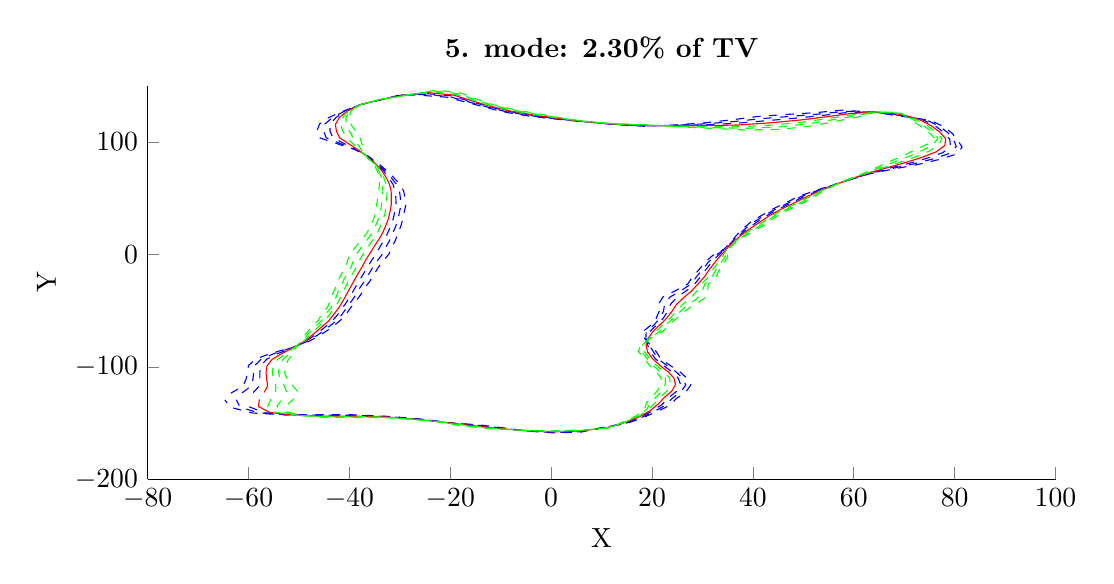
\begin{tikzpicture}

\begin{axis}[%
width=0.95092\figurewidth,
height=\figureheight,
at={(0\figurewidth,0\figureheight)},
scale only axis,
xmin=-80,
xmax=100,
xlabel={X},
ymin=-200,
ymax=150,
ylabel={Y},
title style={font=\bfseries},
title={5. mode: 2.30\% of TV},
axis x line*=bottom,
axis y line*=left
]
\addplot [color=blue,dashed,forget plot]
  table[row sep=crcr]{%
-63.4960537859814	-123.450933424824\\
-61.1288646780023	-117.330368258169\\
-60.4771151161119	-111.056561565406\\
-60.2107416347285	-104.884427212336\\
-60.0168308134828	-98.8853093239553\\
-58.5342739296936	-93.0062980515053\\
-55.4149829950961	-87.839665260832\\
-51.3877345567473	-82.9322727302681\\
-48.1483283243992	-77.7027369013285\\
-45.8010157117073	-71.9664003977102\\
-43.8632216941845	-66.1284975443756\\
-42.1700516667356	-60.2143444669188\\
-40.7706436269569	-54.2409313785058\\
-39.8638666756187	-48.1649150691262\\
-38.7976688393691	-42.0843647266461\\
-37.7622808033087	-36.0231034685099\\
-36.9571665218824	-29.9264710338137\\
-35.9425359310959	-23.8886243404155\\
-35.1005954784015	-17.8243424876481\\
-34.297978851657	-11.7575281540111\\
-33.2381131050116	-5.75370130269225\\
-32.1642899796834	0.257888979517628\\
-31.5731233747559	6.34043942668511\\
-30.8810456901853	12.4146121968997\\
-30.3890849546428	18.6039813779917\\
-29.8125875671942	24.868464556142\\
-29.4078567655912	31.1490604906841\\
-29.1269155050884	37.4337185481654\\
-28.8116754876418	43.7149961746574\\
-28.986725212383	50.0018801427747\\
-29.2362539097101	56.2842393875704\\
-30.0292916836278	62.5450230949333\\
-31.3529822488295	68.7667066400937\\
-32.7479414268541	74.9991689546266\\
-34.4095001916126	81.1820638956\\
-36.2890171763011	87.3081031690781\\
-38.9481888480167	93.1236750368528\\
-42.4890560452009	98.4083647572613\\
-45.9276512503745	103.598926251446\\
-46.4166927954234	109.792415724752\\
-45.9147410667878	115.893877323541\\
-44.0052994799891	121.785678667049\\
-41.0811109044149	127.489161535894\\
-37.9792499957231	132.897287762309\\
-33.6947750739987	137.334158422878\\
-30.0216545464647	141.710767456727\\
-25.9114392234396	141.355450172011\\
-20.7964670962967	139.716687879794\\
-17.1962102952292	135.66415129107\\
-13.4105073315585	131.117701533226\\
-9.37775083110054	126.54111931042\\
-4.48435576004789	122.928590020215\\
1.04132567985193	120.138740237297\\
6.70400984031493	117.705262179571\\
12.4536196837937	115.434856583662\\
18.3914791954511	113.835235631448\\
24.360616739856	114.938546072892\\
30.1785052859887	116.755044942539\\
35.7036211815924	119.478495339856\\
40.9471187062978	122.522849479506\\
46.603698110386	124.304965896834\\
52.2384432790448	125.849944352318\\
57.6936534047031	128.139724852522\\
64.1386552977296	126.203555849173\\
69.6652620731027	122.60230173052\\
75.1504816201084	119.107267873273\\
77.8414127854252	113.554045500231\\
79.4997787278932	107.60753206619\\
80.5790004758853	101.49108605168\\
81.4754282749887	95.344980200789\\
80.4834158841461	89.2511835953983\\
76.8949359998775	84.2387550219722\\
72.6451429018032	79.7619781949701\\
67.8548906291378	75.7921904657889\\
63.2513526377966	71.6441029701645\\
59.6073735400767	66.7481750511897\\
55.9905831064321	61.8118889734646\\
52.5112347189985	56.782887615369\\
49.1428033394768	51.6513992094257\\
46.6429206256224	46.1073605199665\\
44.0789701194388	40.5401532727031\\
41.8057206399753	34.7700267158127\\
39.651691544868	28.9540123718943\\
38.0771007709644	22.9972336642889\\
36.7628565067879	16.9349819617169\\
35.6392658721595	10.8118821978882\\
34.341324325611	4.76584859987374\\
32.0032942109552	-1.12247287766871\\
30.4664242703993	-7.27461065054223\\
29.3251905071082	-13.5918104475523\\
28.0566298482404	-19.8455758892226\\
27.1213608438883	-26.2157106507044\\
24.740361864469	-32.1286682554654\\
22.176332249147	-37.8566444021806\\
21.3002954248608	-44.2212243691237\\
21.4291465101117	-50.7263696326552\\
20.8119447390264	-56.9967903604112\\
19.7673833464916	-63.0139648333557\\
18.1570043586914	-68.8221796810953\\
18.5527778113963	-74.8977579387517\\
19.7803820688601	-81.1211531180436\\
20.9374097442761	-87.1474474344677\\
21.7409679700667	-93.0377811571223\\
23.618291590268	-98.9046426460376\\
25.579497704013	-104.656011845577\\
26.8878817302376	-110.037505734348\\
27.7038214379654	-116.114893746695\\
26.7187878903523	-122.417604926328\\
24.7944613702997	-128.398458988921\\
23.527545017107	-134.322884651859\\
20.8453949843377	-140.063446615275\\
17.9373021552353	-145.70288199329\\
14.8333786001852	-150.601134952305\\
10.1644940329312	-153.954422098224\\
6.05238732623248	-157.924035781089\\
0.551514359331234	-158.77859057244\\
-4.49323256662404	-157.216129354283\\
-9.32435255394677	-154.409226843809\\
-14.293474386606	-151.638002734781\\
-19.7019108943948	-150.021691611318\\
-25.1982567598237	-146.711824700352\\
-31.8239421147606	-144.220016061762\\
-38.7477421457406	-142.707490997783\\
-45.7959606780664	-142.547113102377\\
-52.6228759117609	-142.721607468196\\
-59.126254406127	-141.138229364983\\
-63.5616571912387	-136.065769762401\\
-64.685352575904	-129.447478908625\\
};
\addplot [color=blue,dashed,forget plot]
  table[row sep=crcr]{%
-61.2857308762709	-123.208962737318\\
-59.4885864130844	-117.198940784522\\
-59.1153561019847	-111.045889145992\\
-58.9817190935625	-104.96153695608\\
-58.7930818929718	-99.0018719961739\\
-57.4676842226952	-93.159098661476\\
-54.7008612009195	-87.8815038666312\\
-51.2415285613679	-82.8091777322765\\
-48.354029578036	-77.4792523468864\\
-46.2670045540613	-71.7056116234921\\
-44.4652599932724	-65.8580368666548\\
-42.8345522812882	-59.960962136242\\
-41.5498288365736	-53.9872187685318\\
-40.6055407790025	-47.9421459274899\\
-39.6181917468818	-41.8852917619663\\
-38.6868322907649	-35.8352740331535\\
-37.9087209156532	-29.759662722203\\
-36.984537296785	-23.7187464663759\\
-36.1660757546672	-17.6617168461297\\
-35.363698669296	-11.6029826247208\\
-34.4145859137403	-5.56268224763441\\
-33.4144688295778	0.453525093587851\\
-32.7466859282227	6.52202863111318\\
-31.9863053330396	12.5800244960634\\
-31.4004757761089	18.736973729984\\
-30.8113930335279	24.9649603374071\\
-30.366786748873	31.207401890669\\
-30.0701625795496	37.4566828430292\\
-29.7774464791531	43.7034702121065\\
-29.8864715334664	49.9555401854861\\
-30.0623201876502	56.2021945045496\\
-30.7005688708316	62.4331142750286\\
-31.8078896206302	68.6143013430005\\
-33.0258134666838	74.7797982443279\\
-34.518774623911	80.9016250264984\\
-36.2959260325296	86.9538887678178\\
-38.6453873758303	92.7765623481478\\
-41.648189773702	98.2037628161086\\
-44.5848455758403	103.565862006347\\
-45.1354682061856	109.697034270603\\
-44.8668456942183	115.767865694942\\
-43.3356087414609	121.701273105971\\
-40.8556852462364	127.468439676797\\
-37.9457333705182	132.918465104653\\
-33.7409507457146	137.398391498111\\
-29.7861354976832	141.622621797556\\
-25.3901893584934	142.136806273412\\
-20.2941164492439	140.303569609479\\
-16.7758051187163	136.02056410011\\
-13.0718877837657	131.403580167891\\
-9.02929744841299	126.873100013215\\
-4.16776694825816	123.2514748767\\
1.2008444198572	120.317651819633\\
6.74219411951941	117.770012352938\\
12.4456198778493	115.543843699817\\
18.3646321816167	114.07584419817\\
24.4062855956921	114.707689031737\\
30.4257217145035	115.951268699253\\
36.2195521753189	117.980497914849\\
41.7426598514397	120.627811423779\\
47.4682936394622	122.633118714984\\
53.0361698058332	124.663375377131\\
58.2179940711821	127.124222790737\\
64.2167929079241	126.290218393845\\
69.6028719316174	123.166612350434\\
74.4604219624662	119.282552957298\\
77.0291574360284	113.751382891442\\
78.6986098385452	107.882609122763\\
79.8020742526293	101.860121166964\\
80.3299079851534	95.7867723840221\\
79.085241050624	89.8295062499363\\
75.6983310951099	84.7750617891436\\
71.7009489462542	80.1771983495787\\
67.2641368661037	75.9636409731352\\
62.9848191765114	71.6072685979482\\
59.4443437685391	66.6727849703593\\
55.995066115958	61.6605111118206\\
52.6861374443563	56.5570444515058\\
49.5799937549288	51.3202956101517\\
47.0852627495837	45.7942529998135\\
44.5151989531494	40.2418682740116\\
42.2429913366844	34.4844807883599\\
40.1730227964002	28.6503872497286\\
38.4661861715865	22.7360911603072\\
37.0087687784133	16.7266810524736\\
35.7617798721821	10.6518428723226\\
34.4533731798775	4.61516020799623\\
32.5005252124083	-1.32011082390676\\
31.0906498382484	-7.45747744129007\\
29.9814291661826	-13.7295443328647\\
28.8251520700219	-19.9617364143483\\
27.7939301425105	-26.2550763247273\\
25.7867371492642	-32.2332048972448\\
23.551939905382	-38.0483415989309\\
22.4913078969258	-44.3104155357495\\
22.2746680456714	-50.6947289737082\\
21.5213244862044	-56.9025120637721\\
20.3706457337439	-62.9003860222685\\
18.8395531079369	-68.7467094756525\\
18.7865902650505	-74.7710782004485\\
19.4601845839055	-80.9400443815812\\
20.3269444665544	-86.9964678525753\\
21.1884298198577	-92.9218191330569\\
22.9164227356591	-98.8041865004113\\
24.7826139987202	-104.578071770342\\
26.0434058790806	-110.054618589337\\
26.6882315024378	-116.014229163882\\
25.7950558086939	-122.117791995331\\
24.0132448905548	-128.032741340398\\
22.7602305009938	-133.923758886152\\
20.4570727337136	-139.677962365505\\
17.7816639457971	-145.297475208371\\
14.7696456312883	-150.270599164167\\
10.4671061348256	-153.984197411534\\
6.07677303277342	-157.631601624474\\
0.505571474547682	-158.474586824381\\
-4.75076034613678	-157.073683273368\\
-9.80564995041357	-154.50582469112\\
-14.8839344423266	-151.774617194165\\
-20.2291592122039	-149.781672261666\\
-25.7170345634572	-146.690702173049\\
-32.0940995432981	-144.354526786245\\
-38.7634295761004	-143.113177214435\\
-45.5382425987379	-142.979658915117\\
-52.0566560767359	-142.841044281369\\
-58.005143608921	-140.96165683949\\
-61.7166240107874	-135.816802084846\\
-62.4023896025175	-129.280150050993\\
};
\addplot [color=blue,dashed,forget plot]
  table[row sep=crcr]{%
-59.0754079665604	-122.966992049811\\
-57.8483081481664	-117.067513310875\\
-57.7535970878576	-111.035216726578\\
-57.7526965523965	-105.038646699825\\
-57.5693329724607	-99.1184346683925\\
-56.4010945156968	-93.3118992714467\\
-53.9867394067429	-87.9233424724304\\
-51.0953225659884	-82.6860827342849\\
-48.5597308316729	-77.2557677924443\\
-46.7329933964154	-71.4448228492739\\
-45.0672982923602	-65.5875761889339\\
-43.4990528958408	-59.7075798055652\\
-42.3290140461903	-53.7335061585579\\
-41.3472148823863	-47.7193767858536\\
-40.4387146543944	-41.6862187972865\\
-39.6113837782211	-35.6474445977971\\
-38.860275309424	-29.5928544105923\\
-38.0265386624742	-23.5488685923362\\
-37.2315560309329	-17.4990912046113\\
-36.4294184869351	-11.4484370954306\\
-35.591058722469	-5.37166319257658\\
-34.6646476794722	0.649161207658075\\
-33.9202484816895	6.70361783554124\\
-33.0915649758939	12.7454367952272\\
-32.4118665975751	18.8699660819764\\
-31.8101984998616	25.0614561186721\\
-31.3257167321549	31.265743290654\\
-31.0134096540108	37.4796471378929\\
-30.7432174706644	43.6919442495556\\
-30.7862178545497	49.9092002281975\\
-30.8883864655902	56.1201496215288\\
-31.3718460580354	62.3212054551238\\
-32.2627969924309	68.4618960459074\\
-33.3036855065135	74.5604275340292\\
-34.6280490562095	80.6211861573968\\
-36.302834888758	86.5996743665575\\
-38.3425859036439	92.4294496594429\\
-40.8073235022031	97.9991608749558\\
-43.242039901306	103.532797761247\\
-43.8542436169478	109.601652816454\\
-43.8189503216488	115.641854066343\\
-42.6659180029326	121.616867544894\\
-40.6302595880578	127.447717817699\\
-37.9122167453133	132.939642446997\\
-33.7871264174304	137.462624573344\\
-29.5506164489018	141.534476138384\\
-24.8689394935472	142.918162374813\\
-19.7917658021911	140.890451339163\\
-16.3553999422033	136.376976909151\\
-12.7332682359729	131.689458802556\\
-8.68084406572544	127.205080716011\\
-3.85117813646842	123.574359733185\\
1.36036315986247	120.496563401969\\
6.78037839872389	117.834762526305\\
12.437620071905	115.652830815973\\
18.3377851677824	114.316452764891\\
24.4519544515282	114.476831990583\\
30.6729381430184	115.147492455967\\
36.7354831690455	116.482500489843\\
42.5382009965817	118.732773368053\\
48.3328891685383	120.961271533134\\
53.8338963326215	123.476806401944\\
58.742334737661	126.108720728952\\
64.2949305181187	126.376880938517\\
69.5404817901321	123.730922970348\\
73.7703623048241	119.457838041323\\
76.2169020866317	113.948720282652\\
77.8974409491973	108.157686179337\\
79.0251480293734	102.229156282247\\
79.184387695318	96.2285645672552\\
77.6870662171019	90.4078289044743\\
74.5017261903424	85.3113685563149\\
70.7567549907052	80.5924185041874\\
66.6733831030697	76.1350914804815\\
62.7182857152263	71.5704342257319\\
59.2813139970015	66.5973948895288\\
55.9995491254839	61.5091332501765\\
52.8610401697141	56.3312012876425\\
50.0171841703808	50.9891920108777\\
47.527604873545	45.4811454796605\\
44.95142778686	39.9435832753202\\
42.6802620333935	34.1989348609071\\
40.6943540479324	28.3467621275629\\
38.8552715722086	22.4749486563255\\
37.2546810500386	16.5183801432303\\
35.8842938722047	10.491803546757\\
34.5654220341439	4.46447181611872\\
32.9977562138615	-1.5177487701448\\
31.7148754060976	-7.6403442320379\\
30.637667825257	-13.8672782181771\\
29.5936742918033	-20.0778969394739\\
28.4664994411326	-26.2944419987502\\
26.8331124340594	-32.3377415390242\\
24.927547561617	-38.2400387956813\\
23.6823203689907	-44.3996067023753\\
23.1201895812311	-50.6630883147611\\
22.2307042333823	-56.808233767133\\
20.9739081209962	-62.7868072111814\\
19.5221018571824	-68.6712392702098\\
19.0204027187047	-74.6443984621453\\
19.1399870989509	-80.7589356451189\\
19.7164791888327	-86.8454882706829\\
20.6358916696487	-92.8058571089915\\
22.2145538810502	-98.703730354785\\
23.9857302934275	-104.500131695108\\
25.1989300279236	-110.071731444327\\
25.6726415669102	-115.913564581069\\
24.8713237270354	-121.817979064333\\
23.23202841081	-127.667023691875\\
21.9929159848806	-133.524633120444\\
20.0687504830895	-139.292478115736\\
17.626025736359	-144.892068423451\\
14.7059126623914	-149.940063376029\\
10.76971823672	-154.013972724845\\
6.10115873931435	-157.339167467859\\
0.45962858976413	-158.170583076323\\
-5.00828812564952	-156.931237192453\\
-10.2869473468804	-154.602422538431\\
-15.4743944980471	-151.911231653549\\
-20.7564075300129	-149.541652912013\\
-26.2358123670906	-146.669579645746\\
-32.3642569718356	-144.489037510729\\
-38.7791170064601	-143.518863431088\\
-45.2805245194094	-143.412204727857\\
-51.4904362417109	-142.960481094542\\
-56.884032811715	-140.785084313997\\
-59.8715908303362	-135.567834407291\\
-60.1194266291309	-129.11282119336\\
};
\addplot [color=red,solid,forget plot]
  table[row sep=crcr]{%
-56.8650850568499	-122.725021362305\\
-56.2080298832485	-116.936085837228\\
-56.3918380737305	-111.024544307164\\
-56.5236740112305	-105.115756443569\\
-56.3455840519496	-99.234997340611\\
-55.3345048086984	-93.4646998814174\\
-53.2726176125663	-87.9651810782296\\
-50.949116570609	-82.5629877362933\\
-48.7654320853097	-77.0322832380022\\
-47.1989822387695	-71.1840340750558\\
-45.6693365914481	-65.317115511213\\
-44.1635535103934	-59.4541974748884\\
-43.1081992558071	-53.479793548584\\
-42.0888889857701	-47.4966076442174\\
-41.2592375619071	-41.4871458326067\\
-40.5359352656773	-35.4596151624407\\
-39.8118297031948	-29.4260460989816\\
-39.0685400281634	-23.3789907182966\\
-38.2970363071987	-17.3364655630929\\
-37.4951383045741	-11.2938915661403\\
-36.7675315311977	-5.18064413751875\\
-35.9148265293666	0.844797321728298\\
-35.0938110351563	6.88520703996931\\
-34.1968246187483	12.9108490943909\\
-33.4232574190412	19.0029584339687\\
-32.8090039661952	25.1579518999372\\
-32.2846467154367	31.324084690639\\
-31.956656728472	37.5026114327567\\
-31.7089884621756	43.6804182870047\\
-31.685964175633	49.8628602709089\\
-31.7144527435303	56.038104738508\\
-32.0431232452393	62.209296635219\\
-32.7177043642317	68.3094907488142\\
-33.5815575463431	74.3410568237305\\
-34.737323488508	80.3407472882952\\
-36.3097437449864	86.2454599652972\\
-38.0397844314575	92.082336970738\\
-39.9664572307042	97.794558933803\\
-41.8992342267718	103.499733516148\\
-42.57301902771	109.506271362305\\
-42.7710549490792	115.515842437744\\
-41.9962272644043	121.532461983817\\
-40.4048339298793	127.426995958601\\
-37.8787001201085	132.960819789342\\
-33.8333020891462	137.526857648577\\
-29.3150974001203	141.446330479213\\
-24.3476896286011	143.699518476214\\
-19.2894151551383	141.477333068848\\
-15.9349947656904	136.733389718192\\
-12.3946486881801	131.975337437221\\
-8.33239068303789	127.537061418806\\
-3.53458932467869	123.897244589669\\
1.51988189986774	120.675474984305\\
6.81856267792838	117.899512699672\\
12.4296202659607	115.761817932129\\
18.3109381539481	114.557061331613\\
24.4976233073643	114.245974949428\\
30.9201545715332	114.343716212681\\
37.251414162772	114.984503064837\\
43.3337421417236	116.837735312326\\
49.1974846976144	119.289424351283\\
54.6316228594099	122.290237426758\\
59.2666754041399	125.093218667167\\
64.3730681283133	126.463543483189\\
69.4780916486468	124.295233590262\\
73.0803026471819	119.633123125349\\
75.4046467372349	114.146057673863\\
77.0962720598493	108.43276323591\\
78.2482218061175	102.598191397531\\
78.0388674054827	96.6703567504883\\
76.2888913835798	90.9861515590123\\
73.3051212855748	85.8476753234863\\
69.8125610351563	81.007638658796\\
66.0826293400356	76.3065419878278\\
62.4517522539411	71.5335998535156\\
59.1182842254639	66.5220048086984\\
56.0040321350098	61.3577553885324\\
53.0359428950718	56.1053581237793\\
50.4543745858329	50.6580884116037\\
47.9699469975063	45.1680379595075\\
45.3876566205706	39.6452982766288\\
43.1175327301025	33.9133889334542\\
41.2156852994646	28.0431370053973\\
39.2443569728306	22.2138061523438\\
37.500593321664	16.310079233987\\
36.0068078722273	10.3317642211914\\
34.6774708884103	4.3137834242412\\
33.4949872153146	-1.71538671638284\\
32.3391009739467	-7.82321102278573\\
31.2939064843314	-14.0050121034895\\
30.3621965135847	-20.1940574645996\\
29.1390687397548	-26.3338076727731\\
27.8794877188546	-32.4422781808036\\
26.3031552178519	-38.4317359924316\\
24.8733328410557	-44.4887978690011\\
23.9657111167908	-50.631447655814\\
22.9400839805603	-56.7139554704939\\
21.5771705082485	-62.6732284000942\\
20.2046506064279	-68.595769064767\\
19.2542151723589	-74.5177187238421\\
18.8197896139962	-80.5778269086565\\
19.106013911111	-86.6945086887905\\
20.0833535194397	-92.6898950849261\\
21.5126850264413	-98.6032742091588\\
23.1888465881348	-104.422191619873\\
24.3544541767665	-110.088844299316\\
24.6570516313825	-115.812899998256\\
23.947591645377	-121.518166133336\\
22.4508119310652	-127.301306043352\\
21.2256014687674	-133.125507354736\\
19.6804282324655	-138.906993865967\\
17.4703875269209	-144.486661638532\\
14.6421796934945	-149.609527587891\\
11.0723303386143	-154.043748038156\\
6.12554444585528	-157.046733311244\\
0.413685704980578	-157.866579328265\\
-5.26581590516227	-156.788791111537\\
-10.7682447433472	-154.699020385742\\
-16.0648545537676	-152.047846112932\\
-21.2836558478219	-149.30163356236\\
-26.7545901707241	-146.648457118443\\
-32.6344144003732	-144.623548235212\\
-38.7948044368199	-143.92454964774\\
-45.0228064400809	-143.844750540597\\
-50.924216406686	-143.079917907715\\
-55.7629220145089	-140.608511788504\\
-58.0265576498849	-135.318866729736\\
-57.8364636557443	-128.945492335728\\
};
\addplot [color=green,dashed,forget plot]
  table[row sep=crcr]{%
-54.6547621471394	-122.483050674798\\
-54.5677516183305	-116.804658363581\\
-55.0300790596033	-111.01387188775\\
-55.2946514700645	-105.192866187313\\
-55.1218351314386	-99.3515600128296\\
-54.2679151017	-93.6175004913881\\
-52.5584958183896	-88.0070196840288\\
-50.8029105752295	-82.4398927383016\\
-48.9711333389466	-76.8087986835601\\
-47.6649710811236	-70.9232453008377\\
-46.271374890536	-65.0466548334922\\
-44.828054124946	-59.2008151442116\\
-43.8873844654238	-53.2260809386101\\
-42.8305630891539	-47.2738385025811\\
-42.0797604694197	-41.2880728679269\\
-41.4604867531335	-35.2717857270843\\
-40.7633840969655	-29.2592377873709\\
-40.1105413938525	-23.209112844257\\
-39.3625165834644	-17.1738399215745\\
-38.5608581222132	-11.13934603685\\
-37.9440043399264	-4.98962508246091\\
-37.165005379261	1.04043343579852\\
-36.267373588623	7.06679624439737\\
-35.3020842616026	13.0762613935546\\
-34.4346482405074	19.135950785961\\
-33.8078094325289	25.2544476812023\\
-33.2435766987185	31.3824260906239\\
-32.8999038029332	37.5255757276205\\
-32.6747594536869	43.6688923244539\\
-32.5857104967164	49.8165203136203\\
-32.5405190214703	55.9560598554871\\
-32.7144004324431	62.0973878153143\\
-33.1726117360324	68.157085451721\\
-33.8594295861728	74.1216861134318\\
-34.8465979208064	80.0603084191936\\
-36.3166526012148	85.8912455640368\\
-37.7369829592711	91.7352242820331\\
-39.1255909592053	97.5899569926502\\
-40.5564285522375	103.466669271049\\
-41.2917944384722	109.410889908156\\
-41.7231595765097	115.389830809145\\
-41.326536525876	121.44805642274\\
-40.1794082717008	127.406274099503\\
-37.8451834949036	132.981997131686\\
-33.879477760862	137.59109072381\\
-29.0795783513389	141.358184820042\\
-23.8264397636549	144.480874577615\\
-18.7870645080855	142.064214798532\\
-15.5145895891775	137.089802527233\\
-12.0560291403873	132.261216071886\\
-7.98393730035035	127.869042121601\\
-3.21800051288896	124.220129446154\\
1.67940063987301	120.854386566641\\
6.85674695713286	117.964262873039\\
12.4216204600164	115.870805048285\\
18.2840911401138	114.797669898334\\
24.5432921632004	114.015117908273\\
31.167371000048	113.539939969395\\
37.7673451564986	113.486505639831\\
44.1292832868656	114.942697256599\\
50.0620802266905	117.617577169433\\
55.4293493861982	121.103668451571\\
59.7910160706189	124.077716605381\\
64.4512057385079	126.550206027861\\
69.4157015071615	124.859544210176\\
72.3902429895398	119.808408209374\\
74.5923913878382	114.343395065074\\
76.2951031705014	108.707840292483\\
77.4712955828615	102.967226512814\\
76.8933471156474	97.1121489337214\\
74.8907165500577	91.5644742135503\\
72.1085163808072	86.3839820906577\\
68.8683670796073	81.4228588134047\\
65.4918755770015	76.4779924951741\\
62.185218792656	71.4967654812993\\
58.9552544539263	66.4466147278679\\
56.0085151445357	61.2063775268883\\
53.2108456204296	55.8795149599161\\
50.8915650012849	50.3269848123296\\
48.4122891214676	44.8549304393546\\
45.8238854542812	39.3470132779373\\
43.5548034268116	33.6278430060014\\
41.7370165509969	27.7395118832316\\
39.6334423734527	21.952663648362\\
37.7465055932894	16.1017783247437\\
36.1293218722498	10.1717248956258\\
34.7895197426767	4.16309503236369\\
33.9922182167677	-1.91302466262089\\
32.9633265417959	-8.00607781353357\\
31.9501451434058	-14.1427459888018\\
31.1307187353661	-20.3102179897253\\
29.811638038377	-26.373173346796\\
28.9258630036498	-32.546814822583\\
27.6787628740869	-38.623433189182\\
26.0643453131207	-44.5779890356269\\
24.8112326523505	-50.599806996867\\
23.6494637277383	-56.6196771738547\\
22.1804328955007	-62.559649589007\\
20.8871993556734	-68.5202988593243\\
19.4880276260131	-74.3910389855389\\
18.4995921290416	-80.3967181721942\\
18.4955486333893	-86.5435291068981\\
19.5308153692307	-92.5739330608607\\
20.8108161718324	-98.5028180635325\\
22.391962882842	-104.344251544639\\
23.5099783256095	-110.105957154306\\
23.6414616958549	-115.712235415443\\
23.0238595637186	-121.218353202338\\
21.6695954513203	-126.93558839483\\
20.4582869526542	-132.726381589029\\
19.2921059818414	-138.521509616197\\
17.3147493174827	-144.081254853613\\
14.5784467245976	-149.278991799752\\
11.3749424405087	-154.073523351466\\
6.14993015239621	-156.754299154629\\
0.367742820197026	-157.562575580206\\
-5.52334368467501	-156.646345030622\\
-11.249542139814	-154.795618233053\\
-16.6553146094881	-152.184460572316\\
-21.8109041656309	-149.061614212708\\
-27.2733679743575	-146.62733459114\\
-32.9045718289107	-144.758058959695\\
-38.8104918671797	-144.330235864392\\
-44.7650883607524	-144.277296353337\\
-50.357996571661	-143.199354720888\\
-54.6418112173029	-140.431939263012\\
-56.1815244694336	-135.069899052181\\
-55.5535006823577	-128.778163478096\\
};
\addplot [color=green,dashed,forget plot]
  table[row sep=crcr]{%
-52.4444392374289	-122.241079987292\\
-52.9274733534126	-116.673230889934\\
-53.6683200454762	-111.003199468336\\
-54.0656289288984	-105.269975931057\\
-53.8980862109275	-99.4681226850482\\
-53.2013253947015	-93.7703011013588\\
-51.844374024213	-88.048858289828\\
-50.65670457985	-82.31679774031\\
-49.1768345925834	-76.585314129118\\
-48.1309599234777	-70.6624565266195\\
-46.8734131896238	-64.7761941557713\\
-45.4925547394986	-58.9474328135348\\
-44.6665696750405	-52.9723683286361\\
-43.5722371925377	-47.0510693609448\\
-42.9002833769324	-41.0889999032472\\
-42.3850382405897	-35.0839562917279\\
-41.7149384907363	-29.0924294757602\\
-41.1525427595417	-23.0392349702173\\
-40.4279968597301	-17.0112142800561\\
-39.6265779398523	-10.9848005075598\\
-39.1204771486551	-4.79860602740308\\
-38.4151842291554	1.23606954986874\\
-37.4409361420898	7.24838544882544\\
-36.4073439044569	13.2416736927183\\
-35.4460390619735	19.2689431379533\\
-34.8066148988626	25.3509434624674\\
-34.2025066820003	31.4407674906089\\
-33.8431508773945	37.5485400224842\\
-33.6405304451982	43.657366361903\\
-33.4854568177997	49.7701803563317\\
-33.3665852994104	55.8740149724663\\
-33.3856776196469	61.9854789954095\\
-33.6275191078331	68.0046801546278\\
-34.1373016260024	73.902315403133\\
-34.9558723531049	79.779869550092\\
-36.3235614574432	85.5370311627765\\
-37.4341814870847	91.3881115933281\\
-38.2847246877064	97.3853550514975\\
-39.2136228777033	103.43360502595\\
-40.0105698492344	109.315508454007\\
-40.6752642039402	115.263819180547\\
-40.6568457873477	121.363650861663\\
-39.9539826135223	127.385552240405\\
-37.8116668696987	133.00317447403\\
-33.9256534325779	137.655323799043\\
-28.8440593025574	141.270039160871\\
-23.3051898987087	145.262230679015\\
-18.2847138610327	142.651096528217\\
-15.0941844126645	137.446215336273\\
-11.7174095925945	132.547094706551\\
-7.6354839176628	128.201022824396\\
-2.90141170109923	124.543014302639\\
1.83891937987828	121.033298148977\\
6.89493123633735	118.029013046406\\
12.413620654072	115.97979216444\\
18.2572441262795	115.038278465056\\
24.5889610190366	113.784260867119\\
31.4145874285629	112.736163726109\\
38.2832761502252	111.988508214824\\
44.9248244320075	113.047659200872\\
50.9266757557666	115.945729987583\\
56.2270759129866	119.917099476385\\
60.3153567370978	123.062214543596\\
64.5293433487025	126.636868572533\\
69.3533113656762	125.42385483009\\
71.7001833318976	119.983693293399\\
73.7801360384414	114.540732456284\\
75.4939342811534	108.982917349056\\
76.6943693596056	103.336261628098\\
75.747826825812	97.5539411169545\\
73.4925417165356	92.1427968680883\\
70.9119114760396	86.9202888578291\\
67.9241731240583	81.8380789680134\\
64.9011218139674	76.6494430025204\\
61.9186853313708	71.459931109083\\
58.7922246823887	66.3712246470375\\
56.0129981540615	61.0549996652442\\
53.3857483457874	55.6536717960528\\
51.3287554167369	49.9958812130556\\
48.8546312454289	44.5418229192016\\
46.2601142879918	39.0487282792459\\
43.9920741235207	33.3422970785486\\
42.2583478025291	27.4358867610659\\
40.0225277740748	21.6915211443803\\
37.9924178649147	15.8934774155004\\
36.2518358722724	10.0116855700602\\
34.9015685969431	4.01240664048617\\
34.4894492182209	-2.11066260885893\\
33.587552109645	-8.1889446042814\\
32.6063838024802	-14.2804798741142\\
31.8992409571475	-20.4263785148509\\
30.4842073369991	-26.4125390208189\\
29.972238288445	-32.6513514643624\\
29.0543705303218	-38.8151303859323\\
27.2553577851857	-44.6671802022527\\
25.6567541879102	-50.5681663379199\\
24.3588434749162	-56.5253988772156\\
22.783695282753	-62.4460707779198\\
21.5697481049189	-68.4448286538815\\
19.7218400796673	-74.2643592472357\\
18.179394644087	-80.2156094357318\\
17.8850833556676	-86.3925495250057\\
18.9782772190217	-92.4579710367952\\
20.1089473172235	-98.4023619179062\\
21.5950791775493	-104.266311469404\\
22.6655024744525	-110.123070009296\\
22.6258717603273	-115.61157083263\\
22.1001274820602	-120.91854027134\\
20.8883789715755	-126.569870746307\\
19.6909724365411	-132.327255823321\\
18.9037837312173	-138.136025366428\\
17.1591111080446	-143.675848068694\\
14.5147137557007	-148.948456011614\\
11.6775545424031	-154.103298664777\\
6.17431585893714	-156.461864998014\\
0.321799935413473	-157.258571832148\\
-5.78087146418775	-156.503898949707\\
-11.7308395362808	-154.892216080364\\
-17.2457746652087	-152.3210750317\\
-22.33815248344	-148.821594863055\\
-27.7921457779909	-146.606212063837\\
-33.1747292574483	-144.892569684179\\
-38.8261792975394	-144.735922081045\\
-44.5073702814239	-144.709842166077\\
-49.791776736636	-143.31879153406\\
-53.5207004200969	-140.255366737519\\
-54.3364912889824	-134.820931374626\\
-53.2705377089711	-128.610834620464\\
};
\addplot [color=green,dashed,forget plot]
  table[row sep=crcr]{%
-50.2341163277183	-121.999109299785\\
-51.2871950884946	-116.541803416287\\
-52.3065610313491	-110.992527048921\\
-52.8366063877324	-105.347085674801\\
-52.6743372904164	-99.5846853572668\\
-52.1347356877031	-93.9231017113295\\
-51.1302522300364	-88.0906968956273\\
-50.5104985844706	-82.1937027423184\\
-49.3825358462202	-76.361829574676\\
-48.5969487658318	-70.4016677524014\\
-47.4754514887117	-64.5057334780504\\
-46.1570553540512	-58.694050482858\\
-45.4457548846572	-52.7186557186622\\
-44.3139112959215	-46.8283002193085\\
-43.7208062844451	-40.8899269385674\\
-43.3095897280459	-34.8961268563716\\
-42.6664928845071	-28.9256211641495\\
-42.1945441252308	-22.8693570961777\\
-41.4934771359958	-16.8485886385377\\
-40.6922977574913	-10.8302549782695\\
-40.2969499573838	-4.60758697234524\\
-39.6653630790498	1.43170566393897\\
-38.6144986955566	7.42997465325351\\
-37.5126035473112	13.407085991882\\
-36.4574298834397	19.4019354899456\\
-35.8054203651963	25.4474392437324\\
-35.1614366652821	31.4991088905938\\
-34.7863979518557	37.571504317348\\
-34.6063014367095	43.6458403993521\\
-34.385203138883	49.7238403990431\\
-34.1926515773504	55.7919700894455\\
-34.0569548068507	61.8735701755047\\
-34.0824264796338	67.8522748575346\\
-34.4151736658321	73.6829446928343\\
-35.0651467854034	79.4994306809904\\
-36.3304703136717	85.1828167615162\\
-37.1313800148983	91.0409989046232\\
-37.4438584162074	97.1807531103447\\
-37.870817203169	103.400540780851\\
-38.7293452599966	109.220126999858\\
-39.6273688313707	115.137807551948\\
-39.9871550488195	121.279245300585\\
-39.7285569553438	127.364830381307\\
-37.7781502444939	133.024351816374\\
-33.9718291042937	137.719556874276\\
-28.608540253776	141.1818935017\\
-22.7839400337626	146.043586780416\\
-17.7823632139799	143.237978257901\\
-14.6737792361516	137.802628145314\\
-11.3787900448017	132.832973341216\\
-7.28703053497525	128.533003527191\\
-2.5848228893095	124.865899159124\\
1.99843811988354	121.212209731313\\
6.93311551554183	118.093763219773\\
12.4056208481277	116.088779280596\\
18.2303971124452	115.278887031777\\
24.6346298748727	113.553403825964\\
31.6618038570777	111.932387482823\\
38.7992071439517	110.490510789818\\
45.7203655771495	111.152621145145\\
51.7912712848428	114.273882805733\\
57.0248024397749	118.730530501198\\
60.8396974035767	122.046712481811\\
64.6074809588971	126.723531117205\\
69.2909212241909	125.988165450004\\
71.0101236742555	120.158978377425\\
72.9678806890447	114.738069847495\\
74.6927653918055	109.257994405629\\
75.9174431363497	103.705296743381\\
74.6023065359767	97.9957333001876\\
72.0943668830135	92.7211195226263\\
69.715306571272	87.4565956250005\\
66.9799791685093	82.253299122622\\
64.3103680509334	76.8208935098667\\
61.6521518700857	71.4230967368667\\
58.6291949108511	66.295834566207\\
56.0174811635874	60.9036218036001\\
53.5606510711452	55.4278286321896\\
51.7659458321889	49.6647776137816\\
49.2969733693902	44.2287153990486\\
46.6963431217024	38.7504432805545\\
44.4293448202298	33.0567511510958\\
42.7796790540613	27.1322616389002\\
40.4116131746969	21.4303786403986\\
38.2383301365401	15.6851765062571\\
36.374349872295	9.85164624449466\\
35.0136174512096	3.86171824860866\\
34.986680219674	-2.30830055509698\\
34.2117776774942	-8.37181139502923\\
33.2626224615546	-14.4182137594266\\
32.6677631789289	-20.5425390399766\\
31.1567766356213	-26.4519046948418\\
31.0186135732402	-32.7558881061418\\
30.4299781865568	-39.0068275826827\\
28.4463702572507	-44.7563713688785\\
26.5022757234699	-50.5365256789729\\
25.0682232220942	-56.4311205805765\\
23.3869576700053	-62.3324919668326\\
22.2522968541644	-68.3693584484388\\
19.9556525333215	-74.1376795089324\\
17.8591971591323	-80.0345006992695\\
17.2746180779459	-86.2415699431133\\
18.4257390688127	-92.3420090127298\\
19.4070784626146	-98.30190577228\\
20.7981954722565	-104.18837139417\\
21.8210266232955	-110.140182864285\\
21.6102818247997	-115.510906249817\\
21.1763954004017	-120.618727340343\\
20.1071624918307	-126.204153097784\\
18.9236579204279	-131.928130057613\\
18.5154614805932	-137.750541116659\\
17.0034728986065	-143.270441283775\\
14.4509807868038	-148.617920223476\\
11.9801666442974	-154.133073978088\\
6.19870156547807	-156.169430841399\\
0.275857050629921	-156.954568084089\\
-6.03839924370049	-156.361452868791\\
-12.2121369327476	-154.988813927675\\
-17.8362347209292	-152.457689491084\\
-22.865400801249	-148.581575513402\\
-28.3109235816244	-146.585089536534\\
-33.4448866859858	-145.027080408662\\
-38.8418667278992	-145.141608297697\\
-44.2496522020954	-145.142387978817\\
-49.2255569016111	-143.438228347233\\
-52.3995896228908	-140.078794212026\\
-52.4914581085311	-134.571963697071\\
-50.9875747355845	-128.443505762832\\
};
\end{axis}
\end{tikzpicture}%
					\caption{Modus 5}
					\label{fig:mode5}
				\end{subfigure}	
				\quad
				\begin{subfigure}{0.3\textwidth}
					\centering
					% This file was created by matlab2tikz.
% Minimal pgfplots version: 1.3
%
%The latest updates can be retrieved from
%  http://www.mathworks.com/matlabcentral/fileexchange/22022-matlab2tikz
%where you can also make suggestions and rate matlab2tikz.
%
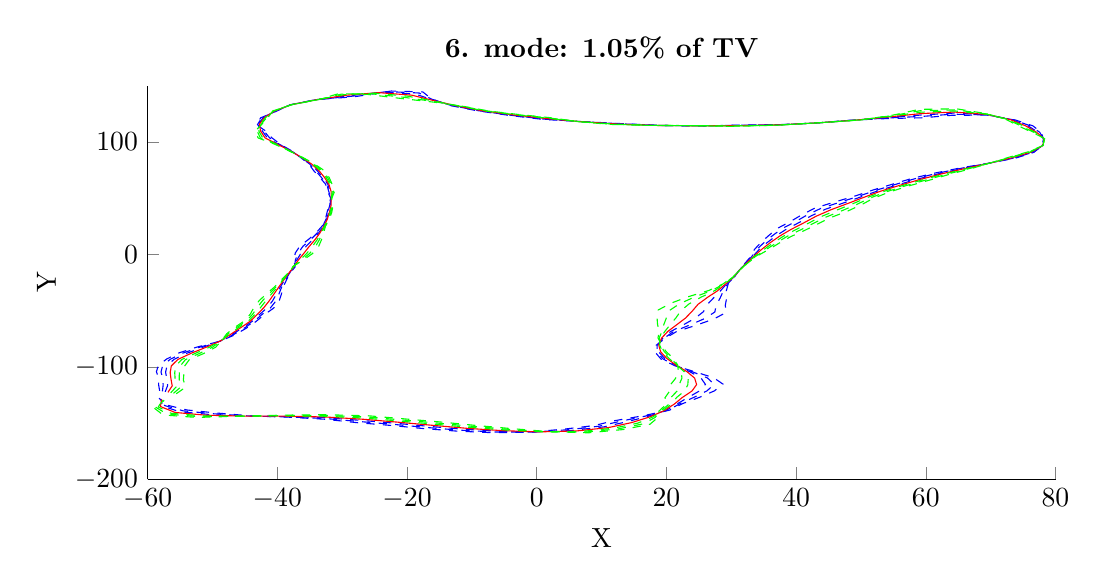
\begin{tikzpicture}

\begin{axis}[%
width=0.95092\figurewidth,
height=\figureheight,
at={(0\figurewidth,0\figureheight)},
scale only axis,
xmin=-60,
xmax=80,
xlabel={X},
ymin=-200,
ymax=150,
ylabel={Y},
title style={font=\bfseries},
title={6. mode: 1.05\% of TV},
axis x line*=bottom,
axis y line*=left
]
\addplot [color=blue,dashed,forget plot]
  table[row sep=crcr]{%
-58.1433893783074	-121.446214404787\\
-58.3066598828725	-115.873903152048\\
-58.2978431884396	-110.120086081553\\
-58.6408322011441	-104.381803260625\\
-58.3484918882549	-98.6777775390941\\
-57.0763288563457	-93.1474411175058\\
-55.1462862432034	-87.6222879089281\\
-52.3882573397598	-82.4865133539922\\
-48.9389321349024	-77.4682213249766\\
-46.6011070301369	-71.7487684294492\\
-44.818682510133	-65.8495903930307\\
-43.3206702496181	-59.9008693578999\\
-42.0613977835012	-53.8859522904221\\
-40.5807234479512	-47.9103678514672\\
-39.7344332128136	-41.8333326303876\\
-39.3873003138515	-35.6934044189609\\
-39.130306174856	-29.5309504279542\\
-38.6346964076717	-23.4000320175901\\
-38.1262369767625	-17.2838210283377\\
-37.2500598689673	-11.2026878134897\\
-37.4408426650718	-4.95419955359849\\
-37.226007424455	1.17989327907419\\
-36.518956748104	7.2945003304358\\
-35.1767316577814	13.2866504010812\\
-33.9744192854766	19.3266061772086\\
-33.0398320302899	25.4202316106028\\
-32.5687259435314	31.5507739295186\\
-32.3119941755743	37.6956388117608\\
-32.0121381738477	43.839637740016\\
-31.7714673045923	49.9811900409185\\
-32.264449348859	56.1159496602038\\
-32.5455002364721	62.2628284743836\\
-33.4276412805293	68.2482442124241\\
-34.3535799502778	74.0991261572325\\
-35.1099185411976	80.0108923840154\\
-36.3550855807537	85.852226106295\\
-37.7100091180494	91.7114302411673\\
-39.4978471484326	97.6241988176101\\
-40.8372634415097	103.567568340477\\
-41.7491166215791	109.356962374194\\
-43.2040948566353	115.248355423711\\
-42.5621247408248	121.331513295019\\
-40.1631227298701	127.089136738866\\
-38.0888611892808	132.833644237325\\
-34.0940975223329	137.449182872759\\
-28.084464360506	140.071658671834\\
-22.4314268982284	145.138346710451\\
-17.5688799904794	144.354725416162\\
-16.2665122854423	138.390687476221\\
-13.6449836294693	132.58249394325\\
-9.29269506930703	127.709502086581\\
-4.29927683183122	123.5186479739\\
0.984920393915832	119.89740868538\\
7.15529924304676	117.950686744263\\
13.3789029460767	116.066601369053\\
19.6629599224252	114.48496595274\\
25.8895173330369	114.0836784453\\
31.7951531051371	114.955663336907\\
37.6182892596903	115.314380885839\\
43.1269948500326	116.736298544932\\
48.457551431336	119.227530464457\\
54.1946965776901	120.710627189992\\
59.551262553329	121.361206720019\\
64.015389042381	123.591185804495\\
69.4626153707267	123.722930354901\\
73.7522601108682	119.469988340655\\
76.506770739532	114.196485142391\\
77.8104430479459	108.392139061667\\
78.1331592265501	102.416086573651\\
77.9401955447921	96.4677061261401\\
76.6687721250642	90.653713039622\\
73.846758220606	85.5180685893844\\
69.8527503057888	81.1336473958616\\
65.4495778987241	76.8866962047277\\
61.4598102822202	72.3073404561726\\
57.8808476804687	67.4619251568373\\
54.8289252247425	62.2553456741327\\
51.7940670589653	57.0360052198462\\
49.0282031264143	51.6699690836409\\
45.9379702063071	46.4844962325776\\
42.914236787165	41.1088933194437\\
40.8896279970986	35.1464932860916\\
39.1021425715459	29.0777782764979\\
37.1187966824595	23.0568909380697\\
35.8226857699279	16.8901683410833\\
34.6120358471313	10.6823288277057\\
33.5971610362949	4.44600834752387\\
33.0400390497891	-1.81764011921401\\
32.1169415577899	-8.00134529152568\\
31.2151575672971	-14.1515736148083\\
30.4738013716548	-20.2997328588825\\
29.5218780849669	-26.4178501636255\\
29.2302865309874	-32.6896288703668\\
29.2793353312165	-39.0790583374373\\
29.0785890680753	-45.4299200263063\\
29.2176685588257	-51.6586086112177\\
27.3239283574289	-57.5187337489536\\
24.527599395854	-63.171753353387\\
21.522687746311	-68.8310815999531\\
19.8018697871621	-74.7037167623855\\
18.4345689531281	-80.8340119861658\\
18.2742050648638	-87.065546827048\\
19.1637201684851	-93.1613820238966\\
21.3172388542404	-99.0731323705424\\
24.508776364048	-104.659346426178\\
27.3078571322806	-109.811402411618\\
28.7232752427693	-115.414362837109\\
27.4008472785599	-121.408794496764\\
25.1136343321474	-127.146943875368\\
22.5160636665261	-132.693217992835\\
20.4932523452818	-138.558153837269\\
16.2978515004321	-143.666916321671\\
11.8271157227466	-148.109435562035\\
8.83083920052951	-152.28385902977\\
4.27469459558205	-155.404482679512\\
-1.00002633724409	-158.109169695491\\
-6.61491943298658	-158.635322152939\\
-12.2037824648416	-157.234747396824\\
-17.4457441917338	-154.932222333559\\
-22.4586141664984	-152.145022446737\\
-27.6379457059165	-149.701726804929\\
-32.6160086024559	-146.654870004465\\
-38.1460952657197	-144.827494054572\\
-43.8829420703875	-143.722994087198\\
-49.3661413774105	-141.116805050834\\
-53.9002376010927	-138.430179291655\\
-57.0365709238496	-134.071911261643\\
-58.2415372127481	-127.945684148026\\
};
\addplot [color=blue,dashed,forget plot]
  table[row sep=crcr]{%
-57.7172879378216	-121.872483390627\\
-57.6071165496645	-116.227964047108\\
-57.6625081502032	-110.421572156756\\
-57.9351128045062	-104.626454321606\\
-57.6808559428198	-98.8635174729331\\
-56.4957208404633	-93.2531940388097\\
-54.5217300329911	-87.7365856320286\\
-51.9085437500429	-82.5120048147592\\
-48.8810987850382	-77.3229086293185\\
-46.8003987663478	-71.5605236446514\\
-45.1022338705714	-65.6720987657582\\
-43.6016313365432	-59.7519787302294\\
-42.4103316076031	-53.7505660431427\\
-41.0834452938909	-47.7724477823839\\
-40.2427013291781	-41.7179370311273\\
-39.7701786311267	-35.6154746667875\\
-39.3574806843022	-29.4959823182967\\
-38.7793109478356	-23.3930182511589\\
-38.1831700869079	-17.3013692065894\\
-37.3317526808363	-11.2330890643732\\
-37.2164056204471	-5.02968108157191\\
-36.7889471260922	1.06819462662556\\
-36.0439081771214	7.15806923361364\\
-34.8500959781037	13.1613832988511\\
-33.7906986633315	19.2187235961286\\
-32.9628893422584	25.332805040381\\
-32.4740328674998	31.4752108498921\\
-32.1935483598735	37.6312963520927\\
-31.911088269957	43.7865645890123\\
-31.7429662616059	49.9417467842487\\
-32.0811171470828	56.0900013529719\\
-32.3780412393945	62.2449845279954\\
-33.1909956417635	68.2686597245541\\
-34.0962391489662	74.1797697127318\\
-34.9857201903011	80.1208440187754\\
-36.3399716354979	85.9833040592957\\
-37.8199342225188	91.8350658176909\\
-39.6540505091898	97.6809855230077\\
-41.1912537032637	103.544956732367\\
-42.023750756956	109.406732036897\\
-43.0597482207833	115.337517761722\\
-42.3734922486846	121.398496191285\\
-40.2436931298732	127.201756478778\\
-38.0188074995567	132.876036087997\\
-34.0071657112706	137.475074464698\\
-28.4946753737108	140.529882607627\\
-23.070181141686	144.658737299039\\
-18.1423917120324	143.395594633724\\
-16.156006445525	137.838254890212\\
-13.2282053157062	132.38010844124\\
-8.97259360721732	127.652021863989\\
-4.04438099611371	123.644846845823\\
1.1632408958998	120.156764118355\\
7.04305372134063	117.933628729399\\
13.0624753860381	115.965006890079\\
19.2122859995995	114.508997745698\\
25.4255526578127	114.137777280009\\
31.5034869272691	114.751680962165\\
37.4959975607175	115.204421612171\\
43.1959106139296	116.77011080073\\
48.7041958534288	119.248161760066\\
54.3403386715967	121.237163935581\\
59.4564001702659	122.605210702402\\
64.1346154043584	124.548638364059\\
69.4677741300334	123.913698100022\\
73.5282742896394	119.524366602219\\
76.1393960720996	114.179675986215\\
77.5723860519137	108.405680453081\\
78.1715134197392	102.476788181611\\
77.9730861650223	96.5352563342562\\
76.5421452112361	90.7645258794187\\
73.6662125755956	85.6279375007517\\
69.8393538822446	81.0916444835064\\
65.6605950458279	76.6933114657611\\
61.7904576061272	72.0494269219536\\
58.2933265288004	67.1486183741243\\
55.220627528165	61.9561489122659\\
52.2080256710008	56.7257895211572\\
49.5035936128871	51.3326755262952\\
46.6152958033735	46.0456768082209\\
43.7387100649669	40.621028305172\\
41.6322629080999	34.7354585018792\\
39.8066568141855	28.7328978527977\\
37.8273167792499	22.7758626761611\\
36.3819882871733	16.6968053053846\\
35.0769598554966	10.5654739588676\\
33.9572643203333	4.40193337309631\\
33.1916884382976	-1.78355565160362\\
32.1909946965088	-7.94196720194569\\
31.2414072063085	-14.102719777702\\
30.4365997522981	-20.2645077274549\\
29.3942749698962	-26.389836000008\\
28.7800202602765	-32.6071786405124\\
28.2872752934283	-38.8632842224354\\
27.6768369924021	-45.1162126405379\\
27.4670160781474	-51.3162216260832\\
25.8626468984727	-57.2504743228004\\
23.5441230999855	-63.0055783689561\\
21.0833420330166	-68.7526440882244\\
19.6193182488944	-74.6417174162044\\
18.5629758400842	-80.7486169603294\\
18.5514746802795	-86.9418674476288\\
19.4702646188033	-93.0042197109064\\
21.3823875783074	-98.9165129834145\\
24.0687997720769	-104.580294824076\\
26.3233894804426	-109.903883040851\\
27.367867372307	-115.547208557491\\
26.2497620674989	-121.445251708955\\
24.22602686512	-127.198397931363\\
22.0859096006066	-132.837314446802\\
20.222310974343	-138.674433846835\\
16.688696842595	-143.940164760625\\
12.7654703796626	-148.60946623732\\
9.57800291322445	-152.870488699232\\
4.89164454567313	-155.951899556756\\
-0.528788989835868	-158.028306239749\\
-6.16521825704514	-158.019811805805\\
-11.7252698910101	-156.389505059797\\
-16.9854476457451	-153.97076359335\\
-22.0669613936062	-151.197226151945\\
-27.3434938608524	-148.683970242767\\
-32.6221438684283	-145.977762748047\\
-38.3623316560864	-144.526512585628\\
-44.2628968602853	-143.763579571664\\
-49.8854997205023	-141.771176003128\\
-54.5211324055648	-139.156290123938\\
-57.3665664991947	-134.487563084341\\
-58.1065126937468	-128.278953543927\\
};
\addplot [color=blue,dashed,forget plot]
  table[row sep=crcr]{%
-57.2911864973357	-122.298752376466\\
-56.9075732164565	-116.582024942168\\
-57.0271731119669	-110.72305823196\\
-57.2293934078684	-104.871105382587\\
-57.0132199973847	-99.0492574067721\\
-55.9151128245808	-93.3589469601135\\
-53.8971738227787	-87.8508833551291\\
-51.4288301603259	-82.5374962755262\\
-48.823265435174	-77.1775959336604\\
-46.9996905025587	-71.3722788598536\\
-45.3857852310097	-65.4946071384856\\
-43.8825924234683	-59.6030881025589\\
-42.7592654317051	-53.6151797958634\\
-41.5861671398305	-47.6345277133006\\
-40.7509694455426	-41.602541431867\\
-40.153056948402	-35.5375449146141\\
-39.5846551937485	-29.4610142086391\\
-38.9239254879995	-23.3860044847278\\
-38.2401031970533	-17.3189173848412\\
-37.4134454927052	-11.2634903152568\\
-36.9919685758224	-5.10516260954533\\
-36.3518868277294	0.956495974176927\\
-35.5688596061388	7.02163813679147\\
-34.523460298426	13.036116196621\\
-33.6069780411863	19.1108410150486\\
-32.8859466542268	25.2453784701591\\
-32.3793397914682	31.3996477702655\\
-32.0751025441728	37.5669538924247\\
-31.8100383660663	43.7334914380085\\
-31.7144652186194	49.9023035275788\\
-31.8977849453065	56.0640530457399\\
-32.2105822423169	62.2271405816072\\
-32.9543500029976	68.2890752366842\\
-33.8388983476547	74.2604132682311\\
-34.8615218394045	80.2307956535353\\
-36.3248576902422	86.1143820122964\\
-37.9298593269882	91.9587013942144\\
-39.810253869947	97.7377722284054\\
-41.5452439650177	103.522345124258\\
-42.298384892333	109.456501699601\\
-42.9154015849313	115.426680099733\\
-42.1848597565445	121.465479087551\\
-40.3242635298762	127.314376218689\\
-37.9487538098326	132.918427938669\\
-33.9202339002084	137.500966056638\\
-28.9048863869156	140.98810654342\\
-23.7089353851435	144.179127887626\\
-18.7159034335853	142.436463851286\\
-16.0455006056077	137.285822304202\\
-12.8114270019432	132.177722939231\\
-8.65249214512761	127.594541641397\\
-3.7894851603962	123.771045717746\\
1.34156139788377	120.41611955133\\
6.93080819963451	117.916570714536\\
12.7460478259994	115.863412411104\\
18.7616120767738	114.533029538655\\
24.9615879825885	114.191876114719\\
31.2118207494012	114.547698587423\\
37.3737058617448	115.094462338504\\
43.2648263778266	116.803923056528\\
48.9508402755216	119.268793055675\\
54.4859807655033	121.763700681169\\
59.3615377872029	123.849214684784\\
64.2538417663359	125.506090923624\\
69.4729328893401	124.104465845142\\
73.3042884684107	119.578744863784\\
75.7720214046673	114.162866830039\\
77.3343290558815	108.419221844496\\
78.2098676129283	102.537489789571\\
78.0059767852525	96.6028065423722\\
76.4155182974079	90.8753387192155\\
73.4856669305852	85.737806412119\\
69.8259574587004	81.0496415711512\\
65.8716121929318	76.4999267267945\\
62.1211049300341	71.7915133877346\\
58.7058053771322	66.8353115914114\\
55.6123298315874	61.6569521503992\\
52.6219842830363	56.4155738224683\\
49.97898409936	50.9953819689494\\
47.2926214004399	45.6068573838642\\
44.5631833427687	40.1331632909004\\
42.3748978191012	34.3244237176667\\
40.511171056825	28.3880174290975\\
38.5358368760403	22.4948344142524\\
36.9412908044186	16.5034422696858\\
35.541883863862	10.4486190900295\\
34.3173676043718	4.35785839866876\\
33.3433378268061	-1.74947118399323\\
32.2650478352278	-7.88258911236571\\
31.26765684532	-14.0538659405957\\
30.3993981329414	-20.2292825960272\\
29.2666718548255	-26.3618218363906\\
28.3297539895656	-32.524728410658\\
27.2952152556401	-38.6475101074335\\
26.2750849167289	-44.8025052547695\\
25.7163635974691	-50.9738346409486\\
24.4013654395165	-56.9822148966471\\
22.560646804117	-62.8394033845251\\
20.6439963197222	-68.6742065764957\\
19.4367667106267	-74.5797180700232\\
18.6913827270402	-80.663221934493\\
18.8287442956953	-86.8181880682096\\
19.7768090691215	-92.8470573979162\\
21.4475363023743	-98.7598935962866\\
23.6288231801058	-104.501243221975\\
25.3389218286045	-109.996363670084\\
26.0124595018448	-115.680054277874\\
25.098676856438	-121.481708921145\\
23.3384193980926	-127.249851987358\\
21.655755534687	-132.981410900769\\
19.9513696034042	-138.790713856401\\
17.0795421847579	-144.213413199578\\
13.7038250365786	-149.109496912606\\
10.3251666259194	-153.457118368694\\
5.5085944957642	-156.499316434\\
-0.0575516424276451	-157.947442784007\\
-5.7155170811037	-157.404301458671\\
-11.2467573171786	-155.54426272277\\
-16.5251510997564	-153.009304853141\\
-21.6753086207141	-150.249429857153\\
-27.0490420157882	-147.666213680605\\
-32.6282791344007	-145.30065549163\\
-38.5785680464532	-144.225531116684\\
-44.6428516501831	-143.804165056131\\
-50.4048580635941	-142.425546955421\\
-55.1420272100369	-139.882400956221\\
-57.6965620745398	-134.903214907038\\
-57.9714881747455	-128.612222939827\\
};
\addplot [color=red,solid,forget plot]
  table[row sep=crcr]{%
-56.8650850568499	-122.725021362305\\
-56.2080298832485	-116.936085837228\\
-56.3918380737305	-111.024544307164\\
-56.5236740112305	-105.115756443569\\
-56.3455840519496	-99.234997340611\\
-55.3345048086984	-93.4646998814174\\
-53.2726176125663	-87.9651810782296\\
-50.949116570609	-82.5629877362933\\
-48.7654320853097	-77.0322832380022\\
-47.1989822387695	-71.1840340750558\\
-45.6693365914481	-65.317115511213\\
-44.1635535103934	-59.4541974748884\\
-43.1081992558071	-53.479793548584\\
-42.0888889857701	-47.4966076442174\\
-41.2592375619071	-41.4871458326067\\
-40.5359352656773	-35.4596151624407\\
-39.8118297031948	-29.4260460989816\\
-39.0685400281634	-23.3789907182966\\
-38.2970363071987	-17.3364655630929\\
-37.4951383045741	-11.2938915661403\\
-36.7675315311977	-5.18064413751875\\
-35.9148265293666	0.844797321728298\\
-35.0938110351563	6.88520703996931\\
-34.1968246187483	12.9108490943909\\
-33.4232574190412	19.0029584339687\\
-32.8090039661952	25.1579518999372\\
-32.2846467154367	31.324084690639\\
-31.956656728472	37.5026114327567\\
-31.7089884621756	43.6804182870047\\
-31.685964175633	49.8628602709089\\
-31.7144527435303	56.038104738508\\
-32.0431232452393	62.209296635219\\
-32.7177043642317	68.3094907488142\\
-33.5815575463431	74.3410568237305\\
-34.737323488508	80.3407472882952\\
-36.3097437449864	86.2454599652972\\
-38.0397844314575	92.082336970738\\
-39.9664572307042	97.794558933803\\
-41.8992342267718	103.499733516148\\
-42.57301902771	109.506271362305\\
-42.7710549490792	115.515842437744\\
-41.9962272644043	121.532461983817\\
-40.4048339298793	127.426995958601\\
-37.8787001201085	132.960819789342\\
-33.8333020891462	137.526857648577\\
-29.3150974001203	141.446330479213\\
-24.3476896286011	143.699518476214\\
-19.2894151551383	141.477333068848\\
-15.9349947656904	136.733389718192\\
-12.3946486881801	131.975337437221\\
-8.33239068303789	127.537061418806\\
-3.53458932467869	123.897244589669\\
1.51988189986774	120.675474984305\\
6.81856267792838	117.899512699672\\
12.4296202659607	115.761817932129\\
18.3109381539481	114.557061331613\\
24.4976233073643	114.245974949428\\
30.9201545715332	114.343716212681\\
37.251414162772	114.984503064837\\
43.3337421417236	116.837735312326\\
49.1974846976144	119.289424351283\\
54.6316228594099	122.290237426758\\
59.2666754041399	125.093218667167\\
64.3730681283133	126.463543483189\\
69.4780916486468	124.295233590262\\
73.0803026471819	119.633123125349\\
75.4046467372349	114.146057673863\\
77.0962720598493	108.43276323591\\
78.2482218061175	102.598191397531\\
78.0388674054827	96.6703567504883\\
76.2888913835798	90.9861515590123\\
73.3051212855748	85.8476753234863\\
69.8125610351563	81.007638658796\\
66.0826293400356	76.3065419878278\\
62.4517522539411	71.5335998535156\\
59.1182842254639	66.5220048086984\\
56.0040321350098	61.3577553885324\\
53.0359428950718	56.1053581237793\\
50.4543745858329	50.6580884116037\\
47.9699469975063	45.1680379595075\\
45.3876566205706	39.6452982766288\\
43.1175327301025	33.9133889334542\\
41.2156852994646	28.0431370053973\\
39.2443569728306	22.2138061523438\\
37.500593321664	16.310079233987\\
36.0068078722273	10.3317642211914\\
34.6774708884103	4.3137834242412\\
33.4949872153146	-1.71538671638284\\
32.3391009739467	-7.82321102278573\\
31.2939064843314	-14.0050121034895\\
30.3621965135847	-20.1940574645996\\
29.1390687397548	-26.3338076727731\\
27.8794877188546	-32.4422781808036\\
26.3031552178519	-38.4317359924316\\
24.8733328410557	-44.4887978690011\\
23.9657111167908	-50.631447655814\\
22.9400839805603	-56.7139554704939\\
21.5771705082485	-62.6732284000942\\
20.2046506064279	-68.595769064767\\
19.2542151723589	-74.5177187238421\\
18.8197896139962	-80.5778269086565\\
19.106013911111	-86.6945086887905\\
20.0833535194397	-92.6898950849261\\
21.5126850264413	-98.6032742091588\\
23.1888465881348	-104.422191619873\\
24.3544541767665	-110.088844299316\\
24.6570516313825	-115.812899998256\\
23.947591645377	-121.518166133336\\
22.4508119310652	-127.301306043352\\
21.2256014687674	-133.125507354736\\
19.6804282324655	-138.906993865967\\
17.4703875269209	-144.486661638532\\
14.6421796934945	-149.609527587891\\
11.0723303386143	-154.043748038156\\
6.12554444585528	-157.046733311244\\
0.413685704980578	-157.866579328265\\
-5.26581590516227	-156.788791111537\\
-10.7682447433472	-154.699020385742\\
-16.0648545537676	-152.047846112932\\
-21.2836558478219	-149.30163356236\\
-26.7545901707241	-146.648457118443\\
-32.6344144003732	-144.623548235212\\
-38.7948044368199	-143.92454964774\\
-45.0228064400809	-143.844750540597\\
-50.924216406686	-143.079917907715\\
-55.7629220145089	-140.608511788504\\
-58.0265576498849	-135.318866729736\\
-57.8364636557443	-128.945492335728\\
};
\addplot [color=green,dashed,forget plot]
  table[row sep=crcr]{%
-56.438983616364	-123.151290348144\\
-55.5084865500405	-117.290146732288\\
-55.7565030354941	-111.326030382367\\
-55.8179546145926	-105.36040750455\\
-55.6779481065145	-99.42073727445\\
-54.7538967928159	-93.5704528027213\\
-52.6480614023539	-88.0794788013301\\
-50.469402980892	-82.5884791970603\\
-48.7075987354455	-76.8869705423441\\
-47.3982739749804	-70.995789290258\\
-45.9528879518865	-65.1396238839405\\
-44.4445145973185	-59.3053068472179\\
-43.457133079909	-53.3444073013046\\
-42.5916108317097	-47.3586875751341\\
-41.7675056782716	-41.3717502333464\\
-40.9188135829526	-35.3816854102673\\
-40.039004212641	-29.391077989324\\
-39.2131545683273	-23.3719769518654\\
-38.3539694173441	-17.3540137413446\\
-37.5768311164431	-11.3242928170239\\
-36.543094486573	-5.25612566549217\\
-35.4777662310038	0.733098669279668\\
-34.6187624641737	6.74877594314714\\
-33.8701889390705	12.7855819921608\\
-33.2395367968961	18.8950758528887\\
-32.7320612781637	25.0705253297153\\
-32.1899536394051	31.2485216110124\\
-31.8382109127713	37.4382689730887\\
-31.607938558285	43.627345136001\\
-31.6574631326466	49.823417014239\\
-31.531120541754	56.012156431276\\
-31.8756642481616	62.1914526888308\\
-32.4810587254658	68.3299062609442\\
-33.3242167450316	74.4217003792298\\
-34.6131251376114	80.4506989230551\\
-36.2946297997306	86.3765379182979\\
-38.1497095359269	92.2059725472616\\
-40.1226605914614	97.8513456392007\\
-42.2532244885258	103.477121908039\\
-42.8476531630869	109.556041025008\\
-42.6267083132272	115.605004775755\\
-41.8075947722641	121.599444880083\\
-40.4854043298824	127.539615698512\\
-37.8086464303844	133.003211640014\\
-33.746370278084	137.552749240516\\
-29.7253084133251	141.904554415006\\
-24.9864438720586	143.219909064801\\
-19.8629268766913	140.518202286409\\
-15.8244889257731	136.180957132182\\
-11.977870374417	131.772951935211\\
-8.01228922094818	127.479581196214\\
-3.27969348896118	124.023443461593\\
1.69820240185171	120.93483041728\\
6.70631715622225	117.882454684809\\
12.113192705922	115.660223453154\\
17.8602642311224	114.58109312457\\
24.0336586321401	114.300073784137\\
30.6284883936652	114.13973383794\\
37.1291224637993	114.874543791169\\
43.4026579056206	116.871547568124\\
49.4441291197072	119.310055646892\\
54.7772649533165	122.816774172346\\
59.1718130210769	126.337222649549\\
64.4922944902908	127.420996042754\\
69.4832504079535	124.486001335383\\
72.8563168259532	119.687501386913\\
75.0372720698026	114.129248517687\\
76.8582150638171	108.446304627324\\
78.2865759993066	102.658893005491\\
78.0717580257129	96.7379069586043\\
76.1622644697517	91.096964398809\\
73.1245756405643	85.9575442348536\\
69.7991646116121	80.9656357464408\\
66.2936464871394	76.1131572488612\\
62.7823995778481	71.2756863192967\\
59.5307630737956	66.2086980259854\\
56.3957344384322	61.0585586266656\\
53.4499015071074	55.7951424250903\\
50.9297650723057	50.3207948542579\\
48.6472725945727	44.7292185351508\\
46.2121298983724	39.1574332623571\\
43.8601676411038	33.5023541492418\\
41.9201995421042	27.698256581697\\
39.952877069621	21.9327778904351\\
38.0598958389093	16.1167161982882\\
36.4717318805926	10.2149093523533\\
35.0375741724488	4.26970844981365\\
33.6466366038231	-1.68130224877245\\
32.4131541126657	-7.76383293320575\\
31.3201561233428	-13.9561582663832\\
30.324994894228	-20.158832333172\\
29.0114656246841	-26.3057935091556\\
27.4292214481437	-32.3598279509492\\
25.3110951800637	-38.2159618774298\\
23.4715807653825	-44.1750904832327\\
22.2150586361125	-50.2890606706795\\
21.4788025216041	-56.4456960443406\\
20.5936942123799	-62.5070534156632\\
19.7653048931335	-68.5173315530383\\
19.0716636340912	-74.4557193776609\\
18.9481965009523	-80.4924318828201\\
19.3832835265268	-86.5708293093713\\
20.3898979697579	-92.5327327719359\\
21.5778337505083	-98.4466548220309\\
22.7488699961637	-104.343140017771\\
23.3699865249285	-110.181324928549\\
23.3016437609203	-115.945745718639\\
22.7965064343161	-121.554623345526\\
21.5632044640377	-127.352760099347\\
20.7954474028479	-133.269603808703\\
19.4094868615267	-139.023273875533\\
17.8612328690838	-144.759910077486\\
15.5805343504105	-150.109558263176\\
11.8194940513093	-154.630377707618\\
6.74249439594635	-157.594150188489\\
0.884923052388801	-157.785715872522\\
-4.81611472922083	-156.173280764403\\
-10.2897321695157	-153.853778048715\\
-15.6045580077789	-151.086387372724\\
-20.8920030749298	-148.353837267568\\
-26.4601383256599	-145.630700556281\\
-32.6405496663456	-143.946440978795\\
-39.0110408271866	-143.623568178796\\
-45.4027612299787	-143.885336025063\\
-51.4435747497778	-143.734288860009\\
-56.383816818981	-141.334622620788\\
-58.35655322523	-135.734518552434\\
-57.701439136743	-129.278761731629\\
};
\addplot [color=green,dashed,forget plot]
  table[row sep=crcr]{%
-56.0128821758782	-123.577559333983\\
-54.8089432168325	-117.644207627348\\
-55.1211679972577	-111.627516457571\\
-55.1122352179547	-105.605058565531\\
-55.0103121610794	-99.606477208289\\
-54.1732887769335	-93.6762057240252\\
-52.0235051921415	-88.1937765244306\\
-49.9896893911751	-82.6139706578273\\
-48.6497653855812	-76.741657846686\\
-47.5975657111913	-70.8075445054602\\
-46.2364393123248	-64.9621322566679\\
-44.7254756842436	-59.1564162195474\\
-43.806066904011	-53.2090210540252\\
-43.0943326776493	-47.2207675060508\\
-42.2757737946361	-41.2563546340862\\
-41.3016919002279	-35.3037556580939\\
-40.2661787220873	-29.3561098796665\\
-39.3577691084912	-23.3649631854342\\
-38.4109025274894	-17.3715619195964\\
-37.658523928312	-11.3546940679074\\
-36.3186574419483	-5.33160719346558\\
-35.040705932641	0.621400016831038\\
-34.1437138931911	6.61234484632498\\
-33.5435532593928	12.6603148899306\\
-33.055816174751	18.7871932718087\\
-32.6551185901321	24.9830987594935\\
-32.0952605633735	31.1729585313858\\
-31.7197650970705	37.3739265134206\\
-31.5068886543943	43.5742719849972\\
-31.6289620896602	49.7839737575691\\
-31.3477883399778	55.986208124044\\
-31.708205251084	62.1736087424426\\
-32.2444130866999	68.3503217730742\\
-33.06687594372	74.5023439347291\\
-34.4889267867149	80.5606505578151\\
-36.2795158544749	86.5076158712986\\
-38.2596346403963	92.3296081237851\\
-40.2788639522186	97.9081323445983\\
-42.6072147502798	103.454510299929\\
-43.1222872984639	109.605810687712\\
-42.4823616773752	115.694167113767\\
-41.618962280124	121.666427776349\\
-40.5659747298855	127.652235438424\\
-37.7385927406603	133.045603490686\\
-33.6594384670218	137.578640832456\\
-30.1355194265299	142.362778350799\\
-25.6251981155162	142.740299653389\\
-20.4364385982442	139.559071503971\\
-15.7139830858558	135.628524546172\\
-11.561092060654	131.570566433202\\
-7.69218775885847	127.422100973623\\
-3.02479765324367	124.149642333516\\
1.87652290383568	121.194185850256\\
6.59407163451612	117.865396669945\\
11.7967651458833	115.558628974179\\
17.4095903082967	114.605124917528\\
23.569693956916	114.354172618847\\
30.3368222157973	113.935751463198\\
37.0068307648265	114.764584517502\\
43.4715736695176	116.905359823921\\
49.6907735418	119.330686942501\\
54.922907047223	123.343310917935\\
59.0769506380139	127.581226631932\\
64.6115208522682	128.378448602319\\
69.4884091672601	124.676769080503\\
72.6323310047244	119.741879648478\\
74.6698974023702	114.112439361511\\
76.620158067785	108.459846018738\\
78.3249301924957	102.719594613451\\
78.1046486459431	96.8054571667204\\
76.0356375559235	91.2077772386058\\
72.9440299955539	86.067413146221\\
69.7857681880679	80.9236328340857\\
66.5046636342432	75.9197725098946\\
63.1130469017551	71.0177727850777\\
59.9432419221273	65.8953912432724\\
56.7874367418546	60.7593618647988\\
53.8638601191429	55.4849267264013\\
51.4051555587786	49.9835012969122\\
49.324598191639	44.2903991107942\\
47.0366031761743	38.6695682480855\\
44.6028025521051	33.0913193650293\\
42.6247137847438	27.3533761579968\\
40.6613971664114	21.6517496285264\\
38.6191983561547	15.9233531625894\\
36.9366558889579	10.0980544835152\\
35.3976774564873	4.22563347538609\\
33.7982859923316	-1.64721778116206\\
32.4872072513846	-7.70445484362577\\
31.3464057623543	-13.9073044292769\\
30.2877932748712	-20.1236072017443\\
28.8838625096134	-26.2777793455381\\
26.9789551774328	-32.2773777210948\\
24.3190351422756	-38.0001877624279\\
22.0698286897093	-43.8613830974643\\
20.4644061554342	-49.9466736855449\\
20.0175210626479	-56.1774366181873\\
19.6102179165114	-62.3408784312323\\
19.3259591798392	-68.4388940413096\\
18.8891120958235	-74.3937200314798\\
19.0766033879083	-80.4070368569837\\
19.6605531419425	-86.4471499299521\\
20.6964424200761	-92.3755704589457\\
21.6429824745752	-98.290035434903\\
22.3088934041926	-104.26408841567\\
22.3855188730905	-110.273805557782\\
21.946235890458	-116.078591439021\\
21.6454212232551	-121.591080557717\\
20.6755969970103	-127.404214155342\\
20.3652933369283	-133.413700262671\\
19.1385454905879	-139.139553885098\\
18.2520782112467	-145.03315851644\\
16.5188890073265	-150.609588938461\\
12.5666577640042	-155.217007377079\\
7.35944434603743	-158.141567065733\\
1.35616039979702	-157.70485241678\\
-4.36641355327939	-155.557770417269\\
-9.81121959568421	-153.008535711688\\
-15.1442614617901	-150.124928632515\\
-20.5003503020376	-147.406040972776\\
-26.1656864805957	-144.612943994119\\
-32.6466849323181	-143.269333722377\\
-39.2272772175534	-143.322586709852\\
-45.7827160198765	-143.92592150953\\
-51.9629330928696	-144.388659812302\\
-57.0047116234531	-142.060733453071\\
-58.6865488005751	-136.150170375132\\
-57.5664146177418	-129.61203112753\\
};
\addplot [color=green,dashed,forget plot]
  table[row sep=crcr]{%
-55.5867807353923	-124.003828319822\\
-54.1093998836244	-117.998268522408\\
-54.4858329590213	-111.929002532775\\
-54.4065158213168	-105.849709626512\\
-54.3426762156444	-99.792217142128\\
-53.592680761051	-93.7819586453291\\
-51.3989489819291	-88.3080742475312\\
-49.5099758014581	-82.6394621185943\\
-48.591932035717	-76.5963451510279\\
-47.7968574474022	-70.6192997206624\\
-46.5199906727632	-64.7846406293953\\
-45.0064367711687	-59.0075255918769\\
-44.155000728113	-53.0736348067459\\
-43.5970545235889	-47.0828474369675\\
-42.7840419110006	-41.1409590348259\\
-41.6845702175032	-35.2258259059205\\
-40.4933532315335	-29.321141770009\\
-39.5023836486551	-23.3579494190031\\
-38.4678356376348	-17.3891100978481\\
-37.740216740181	-11.3850953187909\\
-36.0942203973235	-5.407088721439\\
-34.6036456342782	0.509701364382408\\
-33.6686653222085	6.47591374950282\\
-33.2169175797151	12.5350477877005\\
-32.8720955526059	18.6793106907288\\
-32.5781759021006	24.8956721892716\\
-32.0005674873419	31.0973954517593\\
-31.6013192813698	37.3095840537526\\
-31.4058387505036	43.5211988339935\\
-31.6004610466738	49.7445305008993\\
-31.1644561382015	55.9602598168121\\
-31.5407462540064	62.1557647960544\\
-32.007767447934	68.3707372852042\\
-32.8095351424085	74.5829874902284\\
-34.3647284358183	80.670602192575\\
-36.2644019092191	86.6386938242994\\
-38.3695597448656	92.4532437003087\\
-40.4350673129758	97.9649190499959\\
-42.9612050120339	103.43189869182\\
-43.3969214338408	109.655580350416\\
-42.3380150415232	115.783329451778\\
-41.4303297879838	121.733410672615\\
-40.6465451298885	127.764855178335\\
-37.6685390509362	133.087995341358\\
-33.5725066559596	137.604532424395\\
-30.5457304397346	142.821002286592\\
-26.2639523589737	142.260690241976\\
-21.0099503197972	138.599940721533\\
-15.6034772459385	135.076091960163\\
-11.1443137468909	131.368180931192\\
-7.37208629676876	127.364620751031\\
-2.76990181752616	124.275841205439\\
2.05484340581965	121.453541283231\\
6.48182611281	117.848338655081\\
11.4803375858446	115.457034495204\\
16.958916385471	114.629156710485\\
23.1057292816918	114.408271453556\\
30.0451560379293	113.731769088456\\
36.8845390658538	114.654625243835\\
43.5404894334147	116.939172079719\\
49.9374179638928	119.35131823811\\
55.0685491411296	123.869847663523\\
58.9820882549509	128.825230614314\\
64.7307472142457	129.335901161884\\
69.4935679265668	124.867536825623\\
72.4083451834957	119.796257910043\\
74.3025227349379	114.095630205335\\
76.3821010717528	108.473387410152\\
78.3632843856849	102.780296221411\\
78.1375392661733	96.8730073748364\\
75.9090106420954	91.3185900784026\\
72.7634843505435	86.1772820575883\\
69.7723717645237	80.8816299217305\\
66.7156807813471	75.726387770928\\
63.4436942256621	70.7598592508587\\
60.355720770459	65.5820844605595\\
57.179139045277	60.460165102932\\
54.2778187311784	55.1747110277124\\
51.8805460452515	49.6462077395664\\
50.0019237887054	43.8515796864375\\
47.8610764539762	38.1817032338139\\
45.3454374631065	32.6802845808169\\
43.3292280273834	27.0084957342966\\
41.3699172632018	21.3707213666178\\
39.1785008734001	15.7299901268906\\
37.4015798973232	9.98119961467713\\
35.7577807405257	4.18155850095854\\
33.9499353808401	-1.61313331355167\\
32.5612603901035	-7.64507675404579\\
31.3726554013657	-13.8584505921707\\
30.2505916555145	-20.0883820703167\\
28.7562593945427	-26.2497651819206\\
26.5286889067219	-32.1949274912404\\
23.3269751044874	-37.784413647426\\
20.6680766140361	-43.5476757116959\\
18.7137536747559	-49.6042867004103\\
18.5562396036917	-55.9091771920341\\
18.6267416206429	-62.1747034468013\\
18.8866134665448	-68.3604565295809\\
18.7065605575557	-74.3317206852986\\
19.2050102748643	-80.3216418311473\\
19.9378227573583	-86.323470550533\\
21.0029868703943	-92.2184081459555\\
21.7081311986422	-98.1334160477751\\
21.8689168122216	-104.185036813568\\
21.4010512212525	-110.366286187015\\
20.5908280199958	-116.211437159403\\
20.4943360121942	-121.627537769907\\
19.7879895299829	-127.455668211337\\
19.9351392710087	-133.557796716638\\
18.8676041196491	-139.255833894664\\
18.6429235534096	-145.306406955394\\
17.4572436642424	-151.109619613746\\
13.3138214766991	-155.803637046541\\
7.9763942961285	-158.688983942977\\
1.82739774720525	-157.623988961038\\
-3.91671237733796	-154.942260070135\\
-9.33270702185272	-152.16329337466\\
-14.6839649158014	-149.163469892306\\
-20.1086975291454	-146.458244677984\\
-25.8712346355316	-143.595187431957\\
-32.6528201982905	-142.592226465959\\
-39.4435136079201	-143.021605240908\\
-46.1626708097743	-143.966506993996\\
-52.4822914359614	-145.043030764596\\
-57.6256064279252	-142.786844285354\\
-59.0165443759202	-136.56582219783\\
-57.4313900987405	-129.945300523431\\
};
\end{axis}
\end{tikzpicture}%
					\caption{Modus 6}
					\label{fig:mode6}
				\end{subfigure}	
				\\
				\begin{subfigure}{0.3\textwidth}
					\centering
					% This file was created by matlab2tikz.
% Minimal pgfplots version: 1.3
%
%The latest updates can be retrieved from
%  http://www.mathworks.com/matlabcentral/fileexchange/22022-matlab2tikz
%where you can also make suggestions and rate matlab2tikz.
%
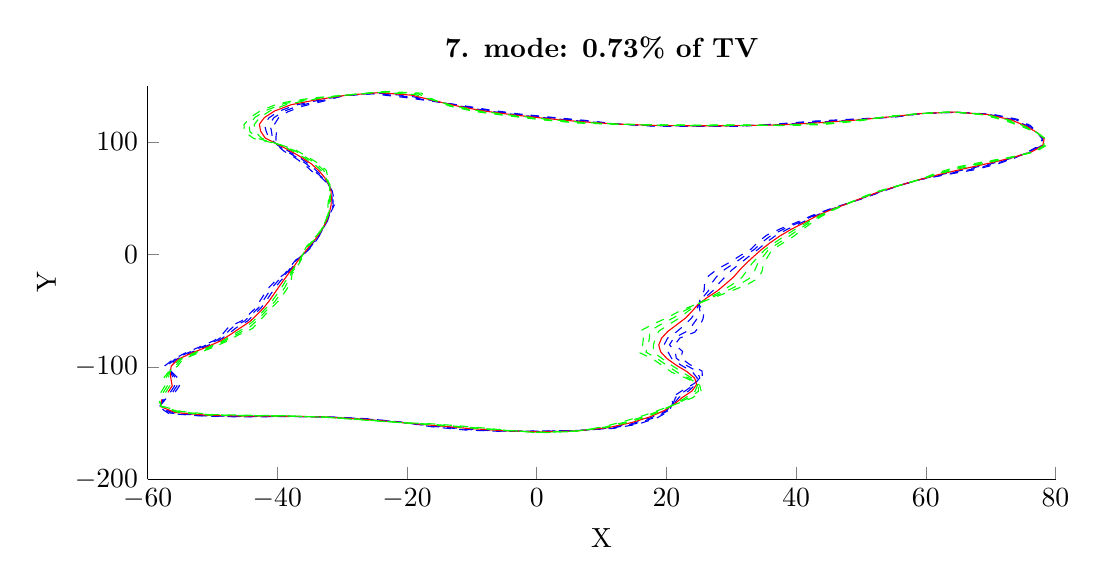
\begin{tikzpicture}

\begin{axis}[%
width=0.95092\figurewidth,
height=\figureheight,
at={(0\figurewidth,0\figureheight)},
scale only axis,
xmin=-60,
xmax=80,
xlabel={X},
ymin=-200,
ymax=150,
ylabel={Y},
title style={font=\bfseries},
title={7. mode: 0.73\% of TV},
axis x line*=bottom,
axis y line*=left
]
\addplot [color=blue,dashed,forget plot]
  table[row sep=crcr]{%
-55.7461779653963	-122.40877110318\\
-55.125420528936	-117.228993119825\\
-55.1590195824485	-111.211815075821\\
-56.1719084650485	-105.063626760447\\
-57.3046819319858	-98.9819095598786\\
-56.0556293214311	-93.4125446251731\\
-54.2000060739503	-87.7512362854111\\
-51.9296245306948	-82.1809177898957\\
-49.6885686959639	-76.5799101678776\\
-48.4071629843296	-70.6987742489154\\
-47.5171435113474	-64.6939395438804\\
-45.4604816670922	-59.0803321560877\\
-44.3379008088029	-53.1935390757443\\
-43.2578404090285	-47.2905912463111\\
-42.6599739336969	-41.3093283837665\\
-41.9925452024709	-35.3463018035167\\
-41.2616547150573	-29.3634286826319\\
-40.2616170888162	-23.3508983587356\\
-38.8755995102423	-17.3916313353542\\
-38.0377475319773	-11.3584171555366\\
-37.1969519778684	-5.23238263321658\\
-35.779209643976	0.72786379342181\\
-34.7010006687578	6.73868773650668\\
-33.925907631852	12.7998814843144\\
-33.256788332826	18.922255901173\\
-32.7258347164848	25.1124601505484\\
-32.1162123157061	31.2965917849714\\
-31.74962416944	37.4961385322038\\
-31.2186075165839	43.6892155734697\\
-31.2942253022681	49.9125943708187\\
-31.5138003998629	56.0951089727333\\
-32.1677908502073	62.2610832279578\\
-33.215603245576	68.266233654975\\
-34.714104765743	74.0221220458326\\
-35.8346478729435	79.9858714340575\\
-37.2743030562547	85.8476163514306\\
-38.9674548962642	91.6558074223079\\
-40.1875565704821	97.7010145218046\\
-40.2113932830634	104.172306981197\\
-40.0832935248109	110.298452728474\\
-40.4032554702796	115.913724922988\\
-39.8081088718521	121.31386284232\\
-38.4102302070171	126.643612255169\\
-36.1392107956027	131.589448936886\\
-32.8494409018818	136.192861880268\\
-29.7774973413107	141.024969975421\\
-25.2919498612789	142.674504770492\\
-20.7379833059349	139.693378251969\\
-15.9603874247225	135.98092930782\\
-11.3349896800882	132.188567041333\\
-7.14458184970983	128.181930311118\\
-2.61030684903879	124.676579583047\\
2.31012099982533	121.785266829733\\
7.32816301870918	119.121297349676\\
12.1662477983612	115.967245786531\\
17.6935490186232	114.001891235602\\
23.8445782265987	113.659629360895\\
30.4099863233997	113.659404980623\\
36.5186811281434	115.627191539997\\
42.6059866698042	118.355341213919\\
48.8641596697015	120.179840275177\\
55.1182037387291	121.890051519459\\
59.3140596973725	125.119205742089\\
64.6978316498292	126.237722003122\\
70.2693451035808	124.498188459462\\
74.0738010834164	120.096249656209\\
76.1266919897362	114.506428591427\\
77.121439685596	108.577654203996\\
77.9644492235601	102.676876556406\\
77.5352435071047	96.718115728128\\
75.7344209446017	91.0747100200007\\
73.6646773448816	85.4758823413295\\
70.9606124644534	80.1120068856026\\
67.5338956030362	75.1706936250539\\
63.3015034295481	70.9312245185259\\
59.1809399262622	66.5456079279827\\
56.0633738770955	61.434236900403\\
53.3639255085614	56.0480709870749\\
50.801066855394	50.6195999044633\\
47.9793356574321	45.3180086549413\\
45.0548640166512	39.9619667273552\\
42.3812290637879	34.3087377779566\\
40.1206453076194	28.4879545783415\\
37.6147340603455	22.7914787281777\\
35.4588350890233	16.9647676535696\\
34.1162716152586	10.9059043907587\\
33.0950890735282	4.79012170555426\\
31.3733428985854	-1.19870424492049\\
29.7195666569418	-7.24709389184638\\
27.8177611405086	-13.2973255680084\\
26.4720028478495	-19.3712865172805\\
25.8783726169071	-25.6251041116437\\
25.8209859941169	-32.1323550160741\\
25.2249744565812	-38.5993802834289\\
25.0238210860585	-44.8846633848066\\
25.8130716475025	-51.111250256089\\
25.6489012364001	-57.2802622784728\\
25.1839373744632	-63.399374281592\\
24.369422369285	-69.2432037469381\\
22.0686043627817	-74.4548554029262\\
21.3024679237787	-80.3655374672622\\
22.486328327083	-86.2907968210383\\
22.2353835692755	-92.272481205195\\
23.5935051081092	-97.9652936567432\\
25.5046024417418	-103.843971679867\\
25.5430808312864	-109.732071597861\\
24.178027177397	-115.245539255042\\
22.5116570661257	-120.902314317913\\
20.901913460371	-126.947816987503\\
20.9218146831455	-133.213632656978\\
20.4145319015154	-139.506474353215\\
18.5157575054239	-145.524545496117\\
15.7500615014143	-150.826917887895\\
11.8192323118747	-154.770748535135\\
6.34100629526626	-156.631873314638\\
0.553668163963366	-157.043261403305\\
-5.37825530454026	-157.459300156573\\
-11.1072072700636	-156.160165557641\\
-16.2343108540497	-153.296631187001\\
-20.811227616999	-149.219601305087\\
-26.2075840861985	-146.14970378712\\
-32.570115351307	-144.437486359881\\
-39.1392159180465	-144.259827785798\\
-45.7707098621411	-144.567291519172\\
-51.9556595317328	-143.665915581115\\
-56.7714148920536	-141.460211956041\\
-58.2225312336708	-135.672977233155\\
-57.1568862279016	-128.284115763759\\
};
\addplot [color=blue,dashed,forget plot]
  table[row sep=crcr]{%
-56.1191469958808	-122.514187856222\\
-55.4862903137068	-117.131357358959\\
-55.5699590795425	-111.149391486268\\
-56.2891636471092	-105.081003321488\\
-56.9849826386404	-99.0662721534561\\
-55.8152544838536	-93.4299297105879\\
-53.8908765868223	-87.8225512163506\\
-51.6027885439995	-82.3082744386949\\
-49.3808564924125	-76.7307011912525\\
-48.0044360691429	-70.8605275242956\\
-46.901207871381	-64.9016648663246\\
-45.028172281526	-59.2049539290213\\
-43.9280002911376	-53.2889572333575\\
-42.8681899346091	-47.3592633789465\\
-42.193061809767	-41.3686008667132\\
-41.5070085568731	-35.384072923158\\
-40.7783797111031	-29.3843011547485\\
-39.8639247352653	-23.3602624785893\\
-38.6827451092277	-17.3732427446005\\
-37.8568777895096	-11.3369086257378\\
-37.0538118289781	-5.21513646798397\\
-35.8244152724395	0.766841636190639\\
-34.8319374575573	6.78752750432755\\
-34.0162132941507	12.8368706876733\\
-33.3122780282311	18.9491567454382\\
-32.7535577997216	25.1276240670114\\
-32.1723571156163	31.3057560868606\\
-31.8186350224507	37.4982961657214\\
-31.3820678317812	43.686283144648\\
-31.4248049267231	49.8960163375154\\
-31.5806845144187	56.0761075613248\\
-32.1262349818846	62.2438210303782\\
-33.0496369517946	68.2806526862547\\
-34.336589025943	74.1284336384653\\
-35.4688730781317	80.1041633854701\\
-36.9527832858319	85.9802308893861\\
-38.6582314079953	91.7979839384513\\
-40.1138567905561	97.7321959924708\\
-40.7740069309662	103.948115826181\\
-40.9132020257772	110.034392273084\\
-41.1925219632128	115.781097427907\\
-40.5374816693695	121.386729222819\\
-39.0750981146379	126.904740156313\\
-36.719040570438	132.046572554371\\
-33.1773946309699	136.637527136371\\
-29.6233640275806	141.165423476685\\
-24.9771964503863	143.016176005733\\
-20.2551272556694	140.288029857596\\
-15.9519232050451	136.231749444611\\
-11.6882093494522	132.117490506629\\
-7.54051812748585	127.966974013681\\
-2.91840100758542	124.416801251921\\
2.04670796650613	121.415336214591\\
7.15829623844891	118.714035799675\\
12.2540386208943	115.898769835064\\
17.8993453970648	114.186947934272\\
24.0622599201873	113.855077890406\\
30.5800424061109	113.887508724642\\
36.7629254730196	115.412962048277\\
42.8485718271107	117.849472580055\\
48.9752680123391	119.883034967213\\
54.9560101122893	122.023446821892\\
59.2982649329616	125.110543383781\\
64.5895771426572	126.312995829811\\
70.0055939519361	124.430536836396\\
73.7426349380049	119.941874145922\\
75.8860102389024	114.386304952239\\
77.1130504770138	108.529357214634\\
78.0590400844126	102.650648170114\\
77.7031181398974	96.7021960689148\\
75.9192444242611	91.0451905330046\\
73.5448253251127	85.5998133353817\\
70.5779286546877	80.4105508100004\\
67.050140182036	75.5493097459786\\
63.0182530376791	71.1320162968558\\
59.1600546926628	66.5377402215546\\
56.0435932964003	61.4087430631128\\
53.2545979707315	56.0671666993097\\
50.6855027655403	50.6324294068434\\
47.9762061041235	45.26801842313\\
45.1657948846243	39.8564105771131\\
42.6266636192261	34.1769548297891\\
40.4856586382345	28.3396820540268\\
38.1579416978406	22.5989212028997\\
36.1394211665702	16.7465381803754\\
34.7464503675815	10.7145243342363\\
33.6225496784889	4.63134227844991\\
32.0805576708285	-1.37093173540794\\
30.5927447626101	-7.43913293549283\\
28.9764762551162	-13.5332210798354\\
27.7687340697612	-19.6455434997202\\
26.965271324523	-25.8613386320202\\
26.5071532356961	-32.2356627376506\\
25.5843680436715	-38.5434988530965\\
24.9736583377242	-44.7527082128714\\
25.1972848039319	-50.9513160559974\\
24.7459621511202	-57.0914933424798\\
23.9816817523916	-63.157325654426\\
22.9811651149993	-69.0273921862144\\
21.1304746326408	-74.4758098432315\\
20.4749084871846	-80.4363006143936\\
21.3595568550923	-86.4253674436224\\
21.5180402193303	-92.4116191651054\\
22.8998984142199	-98.1779538408817\\
24.7326838238728	-104.036711659869\\
25.1468719464464	-109.850995831679\\
24.3377019953922	-115.43465950278\\
22.9903019258762	-121.107598256387\\
21.4182129506024	-127.065646672786\\
21.0230769450195	-133.18425755623\\
20.1698306784987	-139.306647524133\\
18.1673008459229	-145.178584210255\\
15.380767565441	-150.421121121227\\
11.5702649874545	-154.528415036142\\
6.26918567879593	-156.770159980174\\
0.507007344302436	-157.317700711625\\
-5.3407755047476	-157.235797141561\\
-10.9942197611581	-155.673117167008\\
-16.1778254206223	-152.880369495645\\
-20.96870369394	-149.246945390845\\
-26.389919447707	-146.315954897561\\
-32.5915483676624	-144.499506984991\\
-39.024412090971	-144.148068406445\\
-45.5214087214544	-144.326444526313\\
-51.6118451567172	-143.470583023315\\
-56.4352505995387	-141.176311900196\\
-58.1572067057422	-135.554940398682\\
-57.3834120371825	-128.504574621082\\
};
\addplot [color=blue,dashed,forget plot]
  table[row sep=crcr]{%
-56.4921160263654	-122.619604609263\\
-55.8471600984776	-117.033721598094\\
-55.9808985766365	-111.086967896716\\
-56.4064188291698	-105.098379882528\\
-56.665283345295	-99.1506347470336\\
-55.574879646276	-93.4473147960026\\
-53.5817470996943	-87.8938661472901\\
-51.2759525573042	-82.4356310874941\\
-49.0731442888611	-76.8814922146273\\
-47.6017091539562	-71.0222807996757\\
-46.2852722314146	-65.1093901887688\\
-44.5958628959597	-59.3295757019548\\
-43.5180997734723	-53.3843753909707\\
-42.4785394601896	-47.4279355115819\\
-41.726149685837	-41.42787334966\\
-41.0214719112752	-35.4218440427994\\
-40.2951047071489	-29.405173626865\\
-39.4662323817143	-23.3696265984429\\
-38.4898907082132	-17.3548541538467\\
-37.6760080470418	-11.3154000959391\\
-36.9106716800879	-5.19789030275136\\
-35.8696209009031	0.805819478959468\\
-34.9628742463568	6.83636727214843\\
-34.1065189564495	12.8738598910321\\
-33.3677677236361	18.9760575897035\\
-32.7812808829584	25.1427879834743\\
-32.2285019155265	31.3149203887498\\
-31.8876458754614	37.5004537992391\\
-31.5455281469784	43.6833507158264\\
-31.555384551178	49.8794383042122\\
-31.6475686289745	56.0571061499164\\
-32.0846791135619	62.2265588327986\\
-32.8836706580131	68.2950717175344\\
-33.9590732861431	74.2347452310979\\
-35.1030982833198	80.2224553368826\\
-36.6312635154092	86.1128454273416\\
-38.3490079197264	91.9401604545946\\
-40.0401570106301	97.7633774631369\\
-41.336620578869	103.723924671164\\
-41.7431105267436	109.770331817694\\
-41.981788456146	115.648469932825\\
-41.2668544668869	121.459595603318\\
-39.7399660222586	127.165868057457\\
-37.2988703452732	132.503696171856\\
-33.5053483600581	137.082192392474\\
-29.4692307138505	141.305876977949\\
-24.6624430394937	143.357847240973\\
-19.7722712054038	140.882681463222\\
-15.9434589853678	136.482569581401\\
-12.0414290188162	132.046413971925\\
-7.93645440526187	127.752017716243\\
-3.22649516613206	124.157022920795\\
1.78329493318694	121.045405599448\\
6.98842945818865	118.306774249674\\
12.3418294434275	115.830293883596\\
18.1051417755065	114.372004632943\\
24.2799416137758	114.050526419917\\
30.7500984888221	114.115612468662\\
37.0071698178958	115.198732556557\\
43.0911569844171	117.34360394619\\
49.0863763549768	119.586229659248\\
54.7938164858496	122.156842124325\\
59.2824701685508	125.101881025474\\
64.4813226354853	126.3882696565\\
69.7418428002915	124.362885213329\\
73.4114687925934	119.787498635636\\
75.6453284880687	114.266181313051\\
77.1046612684316	108.481060225272\\
78.153630945265	102.624419783822\\
77.87099277269	96.6862764097015\\
76.1040679039204	91.0156710460084\\
73.4249733053437	85.723744329434\\
70.195244844922	80.7090947343982\\
66.5663847610358	75.9279258669032\\
62.7350026458101	71.3328080751857\\
59.1391694590633	66.5298725151265\\
56.023812715705	61.3832492258226\\
53.1452704329017	56.0862624115445\\
50.5699386756866	50.6452589092235\\
47.9730765508149	45.2180281913188\\
45.2767257525975	39.7508544268709\\
42.8720981746643	34.0451718816217\\
40.8506719688496	28.191409529712\\
38.7011493353356	22.4063636776217\\
36.8200072441171	16.5283087071812\\
35.3766291199044	10.5231442777138\\
34.1500102834496	4.47256285134556\\
32.7877724430715	-1.54315922589539\\
31.4659228682784	-7.63117197913928\\
30.1351913697238	-13.7691165916625\\
29.065465291673	-19.9198004821599\\
28.0521700321389	-26.0975731523966\\
27.1933204772754	-32.3389704592271\\
25.9437616307617	-38.4876174227641\\
24.92349558939	-44.6207530409363\\
24.5814979603613	-50.7913818559057\\
23.8430230658402	-56.9027244064868\\
22.7794261303201	-62.9152770272601\\
21.5929078607136	-68.8115806254907\\
20.1923449024998	-74.4967642835368\\
19.6473490505904	-80.5070637615251\\
20.2327853831017	-86.5599380662064\\
20.800696869385	-92.5507571250157\\
22.2062917203306	-98.3906140250202\\
23.9607652060038	-104.229451639871\\
24.7506630616065	-109.969920065498\\
24.4973768133874	-115.623779750518\\
23.4689467856266	-121.312882194861\\
21.9345124408338	-127.183476358069\\
21.1243392068935	-133.154882455483\\
19.9251294554821	-139.10682069505\\
17.8188441864219	-144.832622924394\\
15.0114736294678	-150.015324354559\\
11.3212976630344	-154.286081537149\\
6.19736506232561	-156.908446645709\\
0.460346524641507	-157.592140019945\\
-5.30329570495493	-157.012294126549\\
-10.8812322522526	-155.186068776375\\
-16.121339987195	-152.464107804289\\
-21.126179770881	-149.274289476603\\
-26.5722548092155	-146.482206008002\\
-32.6129813840178	-144.561527610102\\
-38.9096082638954	-144.036309027093\\
-45.2721075807676	-144.085597533455\\
-51.2680307817016	-143.275250465515\\
-56.0990863070238	-140.89241184435\\
-58.0918821778135	-135.436903564209\\
-57.6099378464634	-128.725033478405\\
};
\addplot [color=red,solid,forget plot]
  table[row sep=crcr]{%
-56.8650850568499	-122.725021362305\\
-56.2080298832485	-116.936085837228\\
-56.3918380737305	-111.024544307164\\
-56.5236740112305	-105.115756443569\\
-56.3455840519496	-99.234997340611\\
-55.3345048086984	-93.4646998814174\\
-53.2726176125663	-87.9651810782296\\
-50.949116570609	-82.5629877362933\\
-48.7654320853097	-77.0322832380022\\
-47.1989822387695	-71.1840340750558\\
-45.6693365914481	-65.317115511213\\
-44.1635535103934	-59.4541974748884\\
-43.1081992558071	-53.479793548584\\
-42.0888889857701	-47.4966076442174\\
-41.2592375619071	-41.4871458326067\\
-40.5359352656773	-35.4596151624407\\
-39.8118297031948	-29.4260460989816\\
-39.0685400281634	-23.3789907182966\\
-38.2970363071987	-17.3364655630929\\
-37.4951383045741	-11.2938915661403\\
-36.7675315311977	-5.18064413751875\\
-35.9148265293666	0.844797321728298\\
-35.0938110351563	6.88520703996931\\
-34.1968246187483	12.9108490943909\\
-33.4232574190412	19.0029584339687\\
-32.8090039661952	25.1579518999372\\
-32.2846467154367	31.324084690639\\
-31.956656728472	37.5026114327567\\
-31.7089884621756	43.6804182870047\\
-31.685964175633	49.8628602709089\\
-31.7144527435303	56.038104738508\\
-32.0431232452393	62.209296635219\\
-32.7177043642317	68.3094907488142\\
-33.5815575463431	74.3410568237305\\
-34.737323488508	80.3407472882952\\
-36.3097437449864	86.2454599652972\\
-38.0397844314575	92.082336970738\\
-39.9664572307042	97.794558933803\\
-41.8992342267718	103.499733516148\\
-42.57301902771	109.506271362305\\
-42.7710549490792	115.515842437744\\
-41.9962272644043	121.532461983817\\
-40.4048339298793	127.426995958601\\
-37.8787001201085	132.960819789342\\
-33.8333020891462	137.526857648577\\
-29.3150974001203	141.446330479213\\
-24.3476896286011	143.699518476214\\
-19.2894151551383	141.477333068848\\
-15.9349947656904	136.733389718192\\
-12.3946486881801	131.975337437221\\
-8.33239068303789	127.537061418806\\
-3.53458932467869	123.897244589669\\
1.51988189986774	120.675474984305\\
6.81856267792838	117.899512699672\\
12.4296202659607	115.761817932129\\
18.3109381539481	114.557061331613\\
24.4976233073643	114.245974949428\\
30.9201545715332	114.343716212681\\
37.251414162772	114.984503064837\\
43.3337421417236	116.837735312326\\
49.1974846976144	119.289424351283\\
54.6316228594099	122.290237426758\\
59.2666754041399	125.093218667167\\
64.3730681283133	126.463543483189\\
69.4780916486468	124.295233590262\\
73.0803026471819	119.633123125349\\
75.4046467372349	114.146057673863\\
77.0962720598493	108.43276323591\\
78.2482218061175	102.598191397531\\
78.0388674054827	96.6703567504883\\
76.2888913835798	90.9861515590123\\
73.3051212855748	85.8476753234863\\
69.8125610351563	81.007638658796\\
66.0826293400356	76.3065419878278\\
62.4517522539411	71.5335998535156\\
59.1182842254639	66.5220048086984\\
56.0040321350098	61.3577553885324\\
53.0359428950718	56.1053581237793\\
50.4543745858329	50.6580884116037\\
47.9699469975063	45.1680379595075\\
45.3876566205706	39.6452982766288\\
43.1175327301025	33.9133889334542\\
41.2156852994646	28.0431370053973\\
39.2443569728306	22.2138061523438\\
37.500593321664	16.310079233987\\
36.0068078722273	10.3317642211914\\
34.6774708884103	4.3137834242412\\
33.4949872153146	-1.71538671638284\\
32.3391009739467	-7.82321102278573\\
31.2939064843314	-14.0050121034895\\
30.3621965135847	-20.1940574645996\\
29.1390687397548	-26.3338076727731\\
27.8794877188546	-32.4422781808036\\
26.3031552178519	-38.4317359924316\\
24.8733328410557	-44.4887978690011\\
23.9657111167908	-50.631447655814\\
22.9400839805603	-56.7139554704939\\
21.5771705082485	-62.6732284000942\\
20.2046506064279	-68.595769064767\\
19.2542151723589	-74.5177187238421\\
18.8197896139962	-80.5778269086565\\
19.106013911111	-86.6945086887905\\
20.0833535194397	-92.6898950849261\\
21.5126850264413	-98.6032742091588\\
23.1888465881348	-104.422191619873\\
24.3544541767665	-110.088844299316\\
24.6570516313825	-115.812899998256\\
23.947591645377	-121.518166133336\\
22.4508119310652	-127.301306043352\\
21.2256014687674	-133.125507354736\\
19.6804282324655	-138.906993865967\\
17.4703875269209	-144.486661638532\\
14.6421796934945	-149.609527587891\\
11.0723303386143	-154.043748038156\\
6.12554444585528	-157.046733311244\\
0.413685704980578	-157.866579328265\\
-5.26581590516227	-156.788791111537\\
-10.7682447433472	-154.699020385742\\
-16.0648545537676	-152.047846112932\\
-21.2836558478219	-149.30163356236\\
-26.7545901707241	-146.648457118443\\
-32.6344144003732	-144.623548235212\\
-38.7948044368199	-143.92454964774\\
-45.0228064400809	-143.844750540597\\
-50.924216406686	-143.079917907715\\
-55.7629220145089	-140.608511788504\\
-58.0265576498849	-135.318866729736\\
-57.8364636557443	-128.945492335728\\
};
\addplot [color=green,dashed,forget plot]
  table[row sep=crcr]{%
-57.2380540873344	-122.830438115346\\
-56.5688996680193	-116.838450076362\\
-56.8027775708245	-110.962120717611\\
-56.6409291932911	-105.133133004609\\
-56.0258847586042	-99.3193599341885\\
-55.0941299711208	-93.4820849668322\\
-52.9634881254382	-88.0364960091692\\
-50.6222805839137	-82.6903443850924\\
-48.4577198817583	-77.1830742613771\\
-46.7962553235828	-71.3457873504359\\
-45.0534009514816	-65.5248408336572\\
-43.7312441248271	-59.5788192478219\\
-42.6982987381418	-53.5752117061972\\
-41.6992385113506	-47.5652797768528\\
-40.7923254379771	-41.5464183155535\\
-40.0503986200794	-35.4973862820821\\
-39.3285546992406	-29.4469185710981\\
-38.6708476746124	-23.3883548381503\\
-38.1041819061841	-17.3180769723391\\
-37.3142685621064	-11.2723830363415\\
-36.6243913823075	-5.16339797228614\\
-35.9600321578302	0.883775164497127\\
-35.2247478239557	6.93404680779019\\
-34.287130281047	12.9478382977497\\
-33.4787471144463	19.0298592782339\\
-32.8367270494321	25.1731158164001\\
-32.3407915153469	31.3332489925281\\
-32.0256675814827	37.5047690662743\\
-31.8724487773729	43.6774858581831\\
-31.816543800088	49.8462822376056\\
-31.7813368580861	56.0191033270995\\
-32.0015673769166	62.1920344376394\\
-32.5517380704502	68.3239097800939\\
-33.2040418065432	74.4473684163631\\
-34.3715486936961	80.4590392397078\\
-35.9882239745636	86.3780745032527\\
-37.7305609431886	92.2245134868814\\
-39.8927574507782	97.8257404044691\\
-42.4618478746746	103.275542361132\\
-43.4029275286763	109.242210906915\\
-43.5603214420125	115.383214942663\\
-42.7256000619217	121.605328364316\\
-41.0697018375001	127.688123859744\\
-38.4585298949437	133.417943406827\\
-34.1612558182344	137.97152290468\\
-29.1609640863902	141.586783980477\\
-24.0329362177085	144.041189711454\\
-18.8065591048727	142.071984674474\\
-15.926530546013	136.984209854983\\
-12.7478683575441	131.904260902517\\
-8.72832696081392	127.322105121368\\
-3.84268348322533	123.637466258544\\
1.25646886654854	120.305544369163\\
6.64869589766811	117.492251149671\\
12.5174110884939	115.693341980661\\
18.5167345323898	114.742118030283\\
24.7153050009529	114.441423478939\\
31.0902106542444	114.571819956701\\
37.4956585076483	114.770273573117\\
43.5763272990301	116.331866678461\\
49.308593040252	118.992619043319\\
54.4694292329702	122.423632729191\\
59.2508806397291	125.084556308859\\
64.2648136211414	126.538817309878\\
69.2143404970021	124.227581967196\\
72.7491365017704	119.478747615062\\
75.1639649864012	114.025934034675\\
77.0878828512671	108.384466246547\\
78.3428126669699	102.571963011239\\
78.2067420382754	96.654437091275\\
76.4737148632392	90.9566320720161\\
73.1852692658058	85.9716063175386\\
69.4298772253905	81.3061825831939\\
65.5988739190354	76.6851581087525\\
62.1685018620721	71.7343916318455\\
59.0973989918644	66.5141371022703\\
55.9842515543145	61.3322615512421\\
52.926615357242	56.1244538360141\\
50.3388104959792	50.6709179139838\\
47.9668174441977	45.1180477276963\\
45.4985874885437	39.5397421263866\\
43.3629672855408	33.7816059852868\\
41.5806986300797	27.8948644810825\\
39.7875646103257	22.0212486270658\\
38.1811793992109	16.0918497607928\\
36.6369866245501	10.140384164669\\
35.204931493371	4.15500399713685\\
34.2022019875577	-1.8876142068703\\
33.212279079615	-8.01525006643218\\
32.452621598939	-14.2409076153165\\
31.6589277354964	-20.4683144470393\\
30.2259674473707	-26.5700421931495\\
28.5656549604339	-32.5455859023801\\
26.6625488049421	-38.3758545620992\\
24.8231700927215	-44.356842697066\\
23.3499242732202	-50.4715134557224\\
22.0371448952804	-56.5251865345009\\
20.3749148861769	-62.4311797729282\\
18.8163933521422	-68.3799575040433\\
18.316085442218	-74.5386731641474\\
17.9922301774021	-80.648590055788\\
17.9792424391204	-86.8290793113745\\
19.3660101694944	-92.8290330448364\\
20.819078332552	-98.8159343932973\\
22.4169279702658	-104.614931599875\\
23.9582452919266	-110.207768533135\\
24.8167264493777	-116.002020245994\\
24.4262365051274	-121.72345007181\\
22.9671114212965	-127.419135728636\\
21.3268637306414	-133.096132253989\\
19.4357270094488	-138.707167036884\\
17.1219308674198	-144.140700352671\\
14.2728857575213	-149.203730821222\\
10.8233630141942	-153.801414539162\\
6.05372382938495	-157.18501997678\\
0.367024885319648	-158.141018636585\\
-5.2283361053696	-156.565288096525\\
-10.6552572344417	-154.211971995109\\
-16.0083691203402	-151.631584421576\\
-21.4411319247629	-149.328977648118\\
-26.9369255322326	-146.814708228884\\
-32.6558474167286	-144.685568860322\\
-38.6800006097444	-143.812790268387\\
-44.7735052993942	-143.603903547739\\
-50.5804020316703	-142.884585349915\\
-55.4267577219941	-140.324611732659\\
-57.9612331219563	-135.200829895263\\
-58.0629894650252	-129.165951193051\\
};
\addplot [color=green,dashed,forget plot]
  table[row sep=crcr]{%
-57.6110231178189	-122.935854868388\\
-56.9297694527901	-116.740814315497\\
-57.2137170679184	-110.899697128059\\
-56.7581843753518	-105.15050956565\\
-55.7061854652588	-99.403722527766\\
-54.8537551335432	-93.499470052247\\
-52.6543586383102	-88.1078109401087\\
-50.2954445972184	-82.8177010338916\\
-48.1500076782069	-77.333865284752\\
-46.3935284083962	-71.507540625816\\
-44.4374653115152	-65.7325661561014\\
-43.2989347392609	-59.7034410207555\\
-42.2883982204765	-53.6706298638105\\
-41.3095880369311	-47.6339519094882\\
-40.3254133140472	-41.6056907985002\\
-39.5648619744816	-35.5351574017234\\
-38.8452796952864	-29.4677910432147\\
-38.2731553210615	-23.3977189580039\\
-37.9113275051696	-17.2996883815854\\
-37.1333988196387	-11.2508745065428\\
-36.4812512334172	-5.14615180705352\\
-36.0052377862937	0.922753007265956\\
-35.3556846127552	6.98288657561106\\
-34.3774359433458	12.9848275011085\\
-33.5342368098514	19.0567601224991\\
-32.8644501326689	25.1882797328631\\
-32.396936315257	31.3424132944173\\
-32.0946784344934	37.5069266997919\\
-32.0359090925701	43.6745534293615\\
-31.947123424543	49.8297042043024\\
-31.8482209726418	56.0001019156911\\
-31.9600115085939	62.1747722400598\\
-32.3857717766687	68.3383288113736\\
-32.8265260667432	74.5536800089957\\
-34.0057738988842	80.5773311911203\\
-35.6667042041409	86.5106890412082\\
-37.4213374549197	92.3666900030247\\
-39.8190576708522	97.8569218751353\\
-43.0244615225774	103.051351206116\\
-44.2328360296427	108.978150451525\\
-44.3495879349457	115.250587447582\\
-43.4549728594391	121.678194744815\\
-41.7345697451208	127.949251760888\\
-39.038359669779	133.875067024312\\
-34.4892095473225	138.416188160783\\
-29.0068307726601	141.727237481741\\
-23.7181828068158	144.382860946695\\
-18.3237030546072	142.6666362801\\
-15.9180663263356	137.235029991773\\
-13.101088026908	131.833184367813\\
-9.12426323858994	127.107148823931\\
-4.15077764177196	123.377687927418\\
0.993055833229344	119.93561375402\\
6.47882911740785	117.084989599669\\
12.605201911027	115.624866029194\\
18.7225309108314	114.927174728953\\
24.9329866945414	114.63687200845\\
31.2602667369555	114.799923700721\\
37.7399028525245	114.556044081396\\
43.8189124563366	115.825998044597\\
49.4197013828897	118.695813735354\\
54.3072356065304	122.557028031624\\
59.2350858753182	125.075893950552\\
64.1565591139694	126.614091136567\\
68.9505893453574	124.159930344129\\
72.4179703563589	119.324372104775\\
74.9232832355674	113.905810395487\\
77.0794936426849	108.336169257185\\
78.4374035278224	102.545734624947\\
78.374616671068	96.6385174320618\\
76.6585383428985	90.92711258502\\
73.0654172460369	86.0955373115909\\
69.0471934156248	81.6047265075917\\
65.1151184980351	77.0637742296771\\
61.8852514702031	71.9351834101754\\
59.076513758265	66.5062693958422\\
55.9644709736193	61.3067677139519\\
52.8172878194122	56.1435495482489\\
50.2232464061255	50.6837474163639\\
47.9636878908891	45.068057495885\\
45.6095183565168	39.4341859761445\\
43.608401840979	33.6498230371194\\
41.9457119606948	27.7465919567677\\
40.3307722478207	21.8286911017878\\
38.8617654767578	15.8736202875986\\
37.267165376873	9.94900410814655\\
35.7323920983317	3.99622457003249\\
34.9094167598007	-2.05984169735775\\
34.0854571852833	-8.20728911007863\\
33.6113367135466	-14.4768031271435\\
32.9556589574081	-20.742571429479\\
31.3128661549866	-26.806276713526\\
29.2518222020131	-32.6488936239566\\
27.0219423920324	-38.3199731317668\\
24.7730073443872	-44.2248875251308\\
22.7341374296496	-50.3115792556307\\
21.1342058100004	-56.3364175985079\\
19.1726592641053	-62.1891311457623\\
17.4281360978565	-68.1641459433196\\
17.3779557120771	-74.5596276044527\\
17.1646707408079	-80.7193532029195\\
16.8524709671297	-86.9636499339585\\
18.6486668195491	-92.9681710047467\\
20.1254716386627	-99.0285945774358\\
21.6450093523968	-104.807671579877\\
23.5620364070866	-110.326692766954\\
24.9764012673729	-116.191140493732\\
24.9048813648779	-121.928734010284\\
23.4834109115279	-127.536965413919\\
21.4281259925154	-133.066757153242\\
19.1910257864322	-138.507340207801\\
16.7734742079188	-143.79473906681\\
13.903591821548	-148.797934054554\\
10.5743956897741	-153.559081040169\\
5.98190321291462	-157.323306642315\\
0.320364065658719	-158.415457944904\\
-5.19085630557693	-156.341785081514\\
-10.5422697255362	-153.724923604477\\
-15.9518836869129	-151.21532273022\\
-21.5986080017038	-149.356321733876\\
-27.1192608937411	-146.980959339325\\
-32.677280433084	-144.747589485433\\
-38.5651967826688	-143.701030889035\\
-44.5242041587075	-143.363056554881\\
-50.2365876566547	-142.689252792115\\
-55.0905934294792	-140.040711676813\\
-57.8959085940276	-135.08279306079\\
-58.289515274306	-129.386410050374\\
};
\addplot [color=green,dashed,forget plot]
  table[row sep=crcr]{%
-57.9839921483035	-123.041271621429\\
-57.2906392375609	-116.643178554631\\
-57.6246565650124	-110.837273538507\\
-56.8754395574124	-105.16788612669\\
-55.3864861719134	-99.4880851213434\\
-54.6133802959656	-93.5168551376618\\
-52.3452291511822	-88.1791258710482\\
-49.9686086105232	-82.9450576826908\\
-47.8422954746555	-77.4846563081269\\
-45.9908014932095	-71.6692939011962\\
-43.8215296715488	-65.9402914785456\\
-42.8666253536946	-59.828062793689\\
-41.8784977028113	-53.7660480214237\\
-40.9199375625116	-47.7026240421236\\
-39.8585011901172	-41.664963281447\\
-39.0793253288837	-35.5729285213647\\
-38.3620046913322	-29.4886635153312\\
-37.8754629675105	-23.4070830778576\\
-37.718473104155	-17.2812997908316\\
-36.952529077171	-11.229365976744\\
-36.338111084527	-5.12890564182091\\
-36.0504434147573	0.961730850034786\\
-35.4866214015547	7.03172634343194\\
-34.4677416056445	13.0218167044673\\
-33.5897265052565	19.0836609667644\\
-32.8921732159057	25.203443649326\\
-32.4530811151672	31.3515775963065\\
-32.163689287504	37.5090843333096\\
-32.1993694077674	43.6716210005398\\
-32.077703048998	49.8131261709991\\
-31.9151050871976	55.9811005042826\\
-31.9184556402712	62.1575100424802\\
-32.2198054828873	68.3527478426534\\
-32.4490103269433	74.6599916016283\\
-33.6399991040724	80.6956231425329\\
-35.3451844337181	86.6433035791637\\
-37.1121139666509	92.5088665191681\\
-39.7453578909263	97.8881033458014\\
-43.5870751704802	102.827160051099\\
-45.062744530609	108.714089996135\\
-45.1388544278789	115.1179599525\\
-44.1843456569564	121.751061125314\\
-42.3994376527415	128.210379662032\\
-39.6181894446142	134.332190641797\\
-34.8171632764107	138.860853416886\\
-28.8526974589299	141.867690983005\\
-23.4034293959232	144.724532181935\\
-17.8408470043417	143.261287885726\\
-15.9096021066583	137.485850128564\\
-13.454307696272	131.762107833109\\
-9.52019951636597	126.892192526494\\
-4.4588718003186	123.117909596292\\
0.729642799910147	119.565683138877\\
6.30896233714758	116.677728049668\\
12.6929927335602	115.556390077727\\
18.928327289273	115.112231427623\\
25.1506683881299	114.832320537961\\
31.4303228196667	115.02802744474\\
37.9841471974007	114.341814589676\\
44.0614976136431	115.320129410732\\
49.5308097255273	118.39900842739\\
54.1450419800907	122.690423334057\\
59.2192911109074	125.067231592245\\
64.0483046067975	126.689364963257\\
68.6868381937127	124.092278721062\\
72.0868042109474	119.169996594489\\
74.6826014847337	113.785686756299\\
77.0711044341026	108.287872267823\\
78.5319943886748	102.519506238656\\
78.5424913038607	96.6225977728485\\
76.8433618225579	90.8975930980238\\
72.9455652262679	86.2194683056432\\
68.6645096058591	81.9032704319895\\
64.6313630770349	77.4423903506018\\
61.6020010783341	72.1359751885054\\
59.0556285246655	66.4984016894141\\
55.944690392924	61.2812738766617\\
52.7079602815823	56.1626452604837\\
50.1076823162718	50.696576918744\\
47.9605583375805	45.0180672640738\\
45.7204492244899	39.3286298259023\\
43.8538363964172	33.5180400889519\\
42.3107252913099	27.598319432453\\
40.8739798853157	21.6361335765098\\
39.5423515543047	15.6553908144044\\
37.8973441291959	9.75762405162412\\
36.2598527032924	3.83744514292814\\
35.6166315320438	-2.2320691878452\\
34.9586352909516	-8.39932815372508\\
34.7700518281542	-14.7126986389705\\
34.2523901793198	-21.0168284119187\\
32.3997648626025	-27.0425112339024\\
29.9379894435924	-32.7522013455331\\
27.3813359791226	-38.2640917014344\\
24.722844596053	-44.0929323531957\\
22.1183505860791	-50.151645055539\\
20.2312667247205	-56.147648662515\\
17.9704036420337	-61.9470825185964\\
16.0398788435707	-67.9483343825959\\
16.4398259819362	-74.580582044758\\
16.3371113042137	-80.7901163500509\\
15.7256994951391	-87.0982205565426\\
17.9313234696039	-93.1073089646571\\
19.4318649447734	-99.2412547615743\\
20.8730907345278	-105.000411559879\\
23.1658275222467	-110.445617000772\\
25.1360760853681	-116.38026074147\\
25.3835262246283	-122.134017948759\\
23.9997104017593	-127.654795099202\\
21.5293882543894	-133.037382052495\\
18.9463245634156	-138.307513378718\\
16.4250175484178	-143.448777780948\\
13.5342978855748	-148.392137287886\\
10.325428365354	-153.316747541176\\
5.91008259644429	-157.461593307851\\
0.27370324599779	-158.689897253224\\
-5.15337650578427	-156.118282066502\\
-10.4292822166308	-153.237875213844\\
-15.8953982534855	-150.799061038864\\
-21.7560840786448	-149.383665819634\\
-27.3015962552496	-147.147210449767\\
-32.6987134494394	-144.809610110543\\
-38.4503929555933	-143.589271509682\\
-44.2749030180208	-143.122209562023\\
-49.8927732816391	-142.493920234314\\
-54.7544291369643	-139.756811620968\\
-57.830584066099	-134.964756226317\\
-58.5160410835869	-129.606868907698\\
};
\end{axis}
\end{tikzpicture}%
					\caption{Modus 7}
					\label{fig:mode7}
				\end{subfigure}
				\quad
				\begin{subfigure}{0.3\textwidth}
					\centering
					% This file was created by matlab2tikz.
% Minimal pgfplots version: 1.3
%
%The latest updates can be retrieved from
%  http://www.mathworks.com/matlabcentral/fileexchange/22022-matlab2tikz
%where you can also make suggestions and rate matlab2tikz.
%
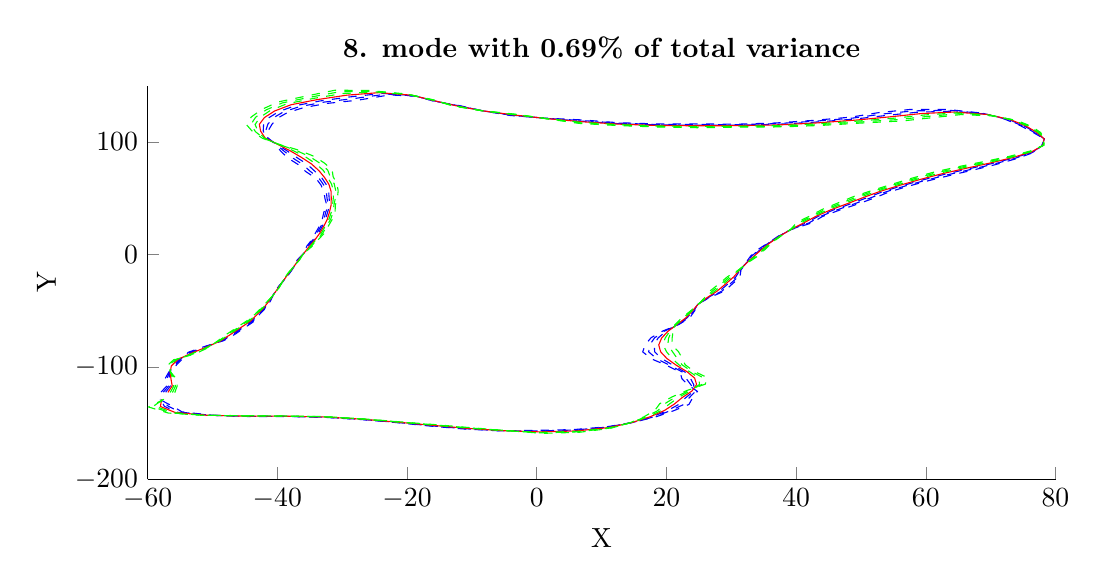
\begin{tikzpicture}

\begin{axis}[%
width=0.95092\figurewidth,
height=\figureheight,
at={(0\figurewidth,0\figureheight)},
scale only axis,
xmin=-60,
xmax=80,
xlabel={X},
ymin=-200,
ymax=150,
ylabel={Y},
title style={font=\bfseries},
title={8. mode with 0.69\% of total variance},
axis x line*=bottom,
axis y line*=left
]
\addplot [color=blue,dashed,forget plot]
  table[row sep=crcr]{%
-57.9142740200415	-122.481157792776\\
-56.9575484458418	-116.509500890685\\
-57.3167946641727	-110.637466228405\\
-56.7262125098687	-104.658290362147\\
-55.626152512264	-98.8596351053894\\
-54.6728239539984	-93.1625000389026\\
-53.7472175976068	-87.1240632532937\\
-51.1537814474026	-81.8535122700385\\
-48.2487703775506	-76.7075767052498\\
-46.5001774047004	-70.9900326687147\\
-45.0107392168143	-65.2104070019058\\
-43.5474305973933	-59.4528739185119\\
-42.7534743712935	-53.5013972425681\\
-41.7501360995133	-47.5871035468258\\
-41.0634201590155	-41.6021295130777\\
-40.6025520486686	-35.6098261560286\\
-39.9530433164668	-29.5480850602404\\
-39.012279437543	-23.4466619425362\\
-38.1609931956808	-17.3391208540415\\
-37.4274957139408	-11.2256562869764\\
-36.9352129532966	-5.05588591967058\\
-35.8741008145569	1.00614659618373\\
-35.464265396802	7.16219464746569\\
-34.6397727008463	13.2539928448762\\
-34.0776427581351	19.3282893991571\\
-33.4683933899422	25.349946408711\\
-33.0615695769812	31.3858451274071\\
-32.819568240941	37.4308239830695\\
-32.3701696774793	43.467586657434\\
-32.6492334320442	49.5149598157104\\
-32.8100741286664	55.5408791067115\\
-33.2676969266181	61.5685349970971\\
-34.0374853964441	67.5729407309179\\
-35.6146954284021	73.5380257936023\\
-36.7477827597957	79.6385300664786\\
-38.3740680628032	85.6254322105859\\
-39.4889249243713	91.7787496264571\\
-40.2948873259746	97.9462640895611\\
-41.5623092113477	104.033455230854\\
-41.3750943728692	110.256304461033\\
-40.7945170782148	115.845897793371\\
-39.9814753291952	120.964726910709\\
-38.4526701856473	125.94194714197\\
-35.9148297543041	130.445705638586\\
-32.3092531378372	134.149342916845\\
-27.5168778717333	137.046018118115\\
-22.684386587942	141.701013389963\\
-18.4259257275851	140.411082165092\\
-15.8570028342164	136.038209079942\\
-11.8278791149653	132.083227400546\\
-8.25841338516549	127.467806683111\\
-4.11295345546496	123.413593481276\\
1.34576176139698	121.002689033582\\
7.10605131003228	119.433418967141\\
12.4055692742789	117.035560275086\\
18.1076821622479	115.955299706342\\
24.2796349203512	115.957507217844\\
30.6511961519635	115.628731081487\\
36.8418634007678	116.72833593989\\
42.7877466376824	119.099441562847\\
48.4421386322795	121.92626822427\\
52.742672508355	125.957663412869\\
57.4982854303684	128.706774683068\\
63.3718758139626	128.753977483177\\
68.7234587454098	125.478889197683\\
72.1362503070668	120.241218121147\\
74.5484139978526	114.451157454653\\
76.4889045398077	108.509968380077\\
78.2870979168217	102.538532109963\\
77.8520706924694	96.3324662700624\\
76.521552924097	90.2638228961665\\
73.7878218249196	84.7104569933096\\
70.6435000150137	79.5707995422816\\
67.246318517138	74.8358252755739\\
63.7460728934231	70.1599619108132\\
60.3697106786068	65.3760247449797\\
57.2206887363502	60.4125384793589\\
54.2955192276813	55.32226337183\\
52.0107666726432	49.9111811823258\\
49.4503292456002	44.6129847735406\\
46.6894102478652	39.2590549988473\\
44.0737748417313	33.6371443114216\\
42.3165632810425	27.7068083069922\\
39.3069350443172	22.1851801605237\\
37.3168584679227	16.3434666042737\\
35.7617202856495	10.3839510113304\\
34.1650420373298	4.45233113359238\\
32.9838087951663	-1.5427791062627\\
32.2250778105304	-7.74756494990538\\
31.4940866480373	-14.0166056737519\\
31.3316670985223	-20.3408059078679\\
30.1380528799047	-26.5085636200985\\
28.9634530188321	-32.6016434234853\\
26.7002378383174	-38.385704938763\\
24.8431434235051	-44.2323057090091\\
24.3400121767337	-50.3453456182244\\
23.5943853228729	-56.5299122927202\\
21.8682445682291	-62.5738329721962\\
19.3868690101584	-68.3299476953669\\
17.6362430127757	-74.1685448027748\\
16.7351195601915	-80.3623359526339\\
16.3466653730163	-86.781907849098\\
17.7333034334889	-93.0530870761006\\
20.1340842516674	-99.0078413010632\\
22.1198017968421	-104.852775017999\\
22.3812767609381	-110.525051016232\\
23.3343034885013	-116.122489426472\\
24.7778520112967	-121.850127964135\\
24.0224396747423	-127.846329267332\\
23.4686108335682	-133.477962127163\\
21.1593739982485	-138.962794660572\\
18.4315257654059	-144.416484045265\\
14.936844921566	-149.314521331392\\
10.7735749289337	-153.373265076031\\
5.69648044302913	-155.833009707503\\
-0.0702489475739101	-156.556693423929\\
-5.82184610325431	-156.922838651082\\
-11.4368773678533	-155.205957507097\\
-16.7138556640304	-152.561290910429\\
-21.7090256355656	-149.558466696235\\
-26.9798930194908	-146.930382157083\\
-32.5300747625573	-144.999461959524\\
-38.2698828992443	-144.171762431953\\
-44.1919242029077	-144.253244040483\\
-50.0606011410349	-143.077130487131\\
-54.7038937889403	-140.093794145392\\
-56.2025750636033	-134.881104607817\\
-58.191595759683	-128.912822571561\\
};
\addplot [color=blue,dashed,forget plot]
  table[row sep=crcr]{%
-57.5645443656443	-122.562445649285\\
-56.7077089249773	-116.651695872866\\
-57.0084758006919	-110.766492254658\\
-56.6586996769893	-104.810779055954\\
-55.8659630254925	-98.9847558504633\\
-54.8933842388984	-93.2632333197409\\
-53.5890176025933	-87.4044358616057\\
-51.0855598218047	-82.0900040921235\\
-48.4209909468037	-76.8158122161673\\
-46.7331123493901	-71.0546998041617\\
-45.2302716750256	-65.2459765050082\\
-43.7528049017267	-59.4533151039707\\
-42.8717159994647	-53.49419601124\\
-41.8630537282656	-47.5569382459563\\
-41.128692626646	-41.5638016195874\\
-40.5803464543382	-35.5597558248326\\
-39.9059721120428	-29.5074054064874\\
-39.0310329677498	-23.4241048677897\\
-38.2063408995201	-17.3382357570586\\
-37.4500432441519	-11.248401380031\\
-36.8793191459303	-5.09747199228663\\
-35.8876760528268	0.952363504698587\\
-35.3407806095868	7.0698654449669\\
-34.4921233401469	13.1396115947144\\
-33.8595143117705	19.2198457440943\\
-33.2485969153599	25.2859482391197\\
-32.8025952897997	31.3652583151511\\
-32.531931070118	37.4547531329652\\
-32.1497759390448	43.5385305339576\\
-32.3281436799072	49.6309266341099\\
-32.4448670002877	55.706620983977\\
-32.8595056994918	61.7821222098044\\
-33.5975583857066	67.81845740355\\
-34.9369828010491	73.805702803645\\
-36.0776296693665	79.8726024737508\\
-37.6859599568643	85.832108128823\\
-39.0058780934	91.879945407884\\
-40.1854106275511	97.8956957043084\\
-41.6746175498224	103.855547992619\\
-41.7744025911494	110.006293428123\\
-41.4533630351696	115.735879341495\\
-40.6530593075982	121.153971935078\\
-39.1033914337247	126.43696341418\\
-36.5694532095722	131.284077022171\\
-32.8172694549402	135.275181160756\\
-28.1162843811956	138.512788905148\\
-23.2388209348284	142.367181752046\\
-18.7137555367695	140.766499133011\\
-15.8830001447077	136.269935959359\\
-12.0168023060369	132.047264079438\\
-8.28307248445629	127.490891595009\\
-3.92016541186953	123.574810517407\\
1.4038018075539	120.893617683823\\
7.01022176599765	118.922116877985\\
12.4135862715062	116.6109794941\\
18.1754341594813	115.489220248099\\
24.3522977160222	115.386996461705\\
30.7408489584868	115.200392791885\\
36.9783803214359	116.147058314873\\
42.9697451390295	118.34553947934\\
48.6939206540578	121.047320266608\\
53.3723226253733	124.735188084165\\
58.0877487549589	127.502256011101\\
63.7056065854128	127.990499483181\\
68.9750030464888	125.084337328543\\
72.4509344204385	120.038519789214\\
74.83382491098	114.349457527723\\
76.6913603798216	108.484233332021\\
78.2741392132536	102.558418539152\\
77.9143362634738	96.4450964302044\\
76.4439990772579	90.5045991171151\\
73.626921645138	85.0895297700352\\
70.3665203550612	80.0497459144531\\
66.8584221247705	75.3260641796585\\
63.3146326802624	70.6178412250473\\
59.9525685275592	65.7580180995526\\
56.8151365359034	60.7276107824167\\
53.8756604501448	55.5832949558131\\
51.4919693103731	50.1601502587518\\
48.9568684962356	44.7980025021963\\
46.2554923721003	39.3878027581078\\
43.7550274711884	33.7292258520992\\
41.9496039538499	27.8189178731272\\
39.286075687155	22.1947221577971\\
37.3781034191698	16.3323374808448\\
35.8434161478421	10.3665554146174\\
34.3358516543567	4.40614856380866\\
33.1542016018824	-1.60031497630275\\
32.2630855316692	-7.77278030753216\\
31.427359926802	-14.0127411503311\\
31.0085102368764	-20.2918897601118\\
29.8050581665214	-26.4503116376567\\
28.6021312521729	-32.5485216759247\\
26.5678769648289	-38.4010486233192\\
24.8532065626886	-44.3178030956731\\
24.2152451567527	-50.4407129640876\\
23.3762848754354	-56.5912600186447\\
21.7712198815689	-62.6069647814955\\
19.6594628755816	-68.4185548185003\\
18.1755670659701	-74.2849361097972\\
17.4300095781264	-80.4341662713081\\
17.2664482190479	-86.7527747956622\\
18.5166534621392	-92.9320230790424\\
20.5936178432587	-98.8729856037617\\
22.4761500606063	-104.709247218624\\
23.0390025662142	-110.37964877726\\
23.7752195361284	-116.0192929504\\
24.5010985559901	-121.739474020535\\
23.4985637601832	-127.664654859339\\
22.7209410453012	-133.360477203021\\
20.6663920763208	-138.944194395704\\
18.1111463525775	-144.439876576354\\
14.8386231788755	-149.412856750225\\
10.8731600654939	-153.59675939674\\
5.83950177730451	-156.237584242083\\
0.0910626032775858	-156.993322058707\\
-5.6365027038903	-156.8781561379\\
-11.2139998263512	-155.036978466645\\
-16.4975219606095	-152.390142644597\\
-21.5672357063177	-149.47285565161\\
-26.9047920699019	-146.836407144203\\
-32.5648546418292	-144.874157384753\\
-38.4448567451028	-144.089358170549\\
-44.4688849486321	-144.117079540521\\
-50.3484728962519	-143.078059627326\\
-55.0569031974632	-140.265366693096\\
-56.8105692590305	-135.027025315124\\
-58.0732183917034	-128.92371249295\\
};
\addplot [color=blue,dashed,forget plot]
  table[row sep=crcr]{%
-57.2148147112471	-122.643733505795\\
-56.4578694041129	-116.793890855047\\
-56.7001569372112	-110.895518280911\\
-56.5911868441099	-104.963267749761\\
-56.1057735387211	-99.1098765955372\\
-55.1139445237984	-93.3639666005792\\
-53.4308176075798	-87.6848084699177\\
-51.0173381962068	-82.3264959142084\\
-48.5932115160567	-76.9240477270848\\
-46.9660472940798	-71.1193669396088\\
-45.4498041332368	-65.2815460081106\\
-43.9581792060601	-59.4537562894296\\
-42.9899576276359	-53.486994779912\\
-41.9759713570178	-47.5267729450868\\
-41.1939650942766	-41.5254737260971\\
-40.5581408600077	-35.5096854936367\\
-39.8589009076188	-29.4667257527345\\
-39.0497864979566	-23.4015477930431\\
-38.2516886033594	-17.3373506600758\\
-37.472590774363	-11.2711464730857\\
-36.823425338564	-5.13905806490269\\
-35.9012512910967	0.898580413213443\\
-35.2172958223715	6.9775362424681\\
-34.3444739794476	13.0252303445526\\
-33.6413858654058	19.1114020890315\\
-33.0288004407776	25.2219500695285\\
-32.5436210026182	31.344671502895\\
-32.244293899295	37.478682282861\\
-31.9293822006102	43.6094744104811\\
-32.0070539277701	49.7468934525094\\
-32.079659871909	55.8723628612425\\
-32.4513144723655	61.9957094225117\\
-33.1576313749691	68.0639740761821\\
-34.2592701736961	74.0733798136878\\
-35.4074765789372	80.106674881023\\
-36.9978518509253	86.0387840470601\\
-38.5228312624288	91.981141189311\\
-40.0759339291276	97.8451273190557\\
-41.7869258882971	103.677640754383\\
-42.1737108094297	109.756282395214\\
-42.1122089921244	115.62586088962\\
-41.3246432860013	121.343216959448\\
-39.754112681802	126.931979686391\\
-37.2240766648403	132.122448405756\\
-33.3252857720432	136.401019404666\\
-28.715690890658	139.97955969218\\
-23.7932552817147	143.03335011413\\
-19.0015853459539	141.121916100929\\
-15.9089974551991	136.501662838775\\
-12.2057254971085	132.011300758329\\
-8.30773158374709	127.513976506907\\
-3.72737736827411	123.736027553538\\
1.46184185371082	120.784546334064\\
6.91439222196301	118.410814788829\\
12.4216032687334	116.186398713114\\
18.2431861567147	115.023140789856\\
24.4249605116933	114.816485705567\\
30.83050176501	114.772054502283\\
37.1148972421039	115.565780689855\\
43.1517436403766	117.591637395833\\
48.9457026758361	120.168372308946\\
54.0019727423916	123.512712755462\\
58.6772120795494	126.297737339134\\
64.0393373568631	127.227021483185\\
69.2265473475678	124.689785459403\\
72.7656185338102	119.835821457281\\
75.1192358241075	114.247757600793\\
76.8938162198355	108.458498283966\\
78.2611805096856	102.578304968341\\
77.9766018344783	96.5577265903463\\
76.3664452304189	90.7453753380637\\
73.4660214653564	85.4686025467607\\
70.0895406951087	80.5286922866245\\
66.470525732403	75.8163030837432\\
62.8831924671018	71.0757205392815\\
59.5354263765115	66.1400114541255\\
56.4095843354566	61.0426830854745\\
53.4558016726083	55.8443265397962\\
50.973171948103	50.4091193351777\\
48.4634077468709	44.9830202308519\\
45.8215744963355	39.5165505173683\\
43.4362801006455	33.8213073927767\\
41.5826446266573	27.9310274392622\\
39.2652163299928	22.2042641550704\\
37.4393483704169	16.3212083574159\\
35.9251120100347	10.3491598179044\\
34.5066612713835	4.35996599402493\\
33.3245944085985	-1.65785084634279\\
32.3010932528079	-7.79799566515895\\
31.3606332055667	-14.0088766269103\\
30.6853533752305	-20.2429736123557\\
29.4720634531381	-26.3920596552149\\
28.2408094855138	-32.4953999283642\\
26.4355160913404	-38.4163923078754\\
24.8632697018722	-44.4033004823371\\
24.0904781367718	-50.5360803099508\\
23.1581844279978	-56.6526077445693\\
21.6741951949087	-62.6400965907949\\
19.9320567410047	-68.5071619416336\\
18.7148911191645	-74.4013274168197\\
18.1248995960613	-80.5059965899823\\
18.1862310650794	-86.7236417422263\\
19.3000034907894	-92.8109590819843\\
21.05315143485	-98.7381299064602\\
22.8324983243705	-104.565719419249\\
23.6967283714904	-110.234246538288\\
24.2161355837554	-115.916096474328\\
24.2243451006836	-121.628820076936\\
22.9746878456242	-127.482980451345\\
21.9732712570343	-133.242992278879\\
20.1734101543931	-138.925594130835\\
17.7907669397492	-144.463269107443\\
14.740401436185	-149.511192169058\\
10.9727452020541	-153.820253717448\\
5.9825231115799	-156.642158776664\\
0.252374154129082	-157.429950693486\\
-5.45115930452628	-156.833473624719\\
-10.9911222848492	-154.867999426194\\
-16.2811882571885	-152.218994378765\\
-21.4254457770698	-149.387244606985\\
-26.829691120313	-146.742432131323\\
-32.5996345211012	-144.748852809983\\
-38.6198305909614	-144.006953909144\\
-44.7458456943565	-143.980915040559\\
-50.6363446514689	-143.07898876752\\
-55.409912605986	-140.4369392408\\
-57.4185634544577	-135.17294602243\\
-57.9548410237239	-128.934602414339\\
};
\addplot [color=red,solid,forget plot]
  table[row sep=crcr]{%
-56.8650850568499	-122.725021362305\\
-56.2080298832485	-116.936085837228\\
-56.3918380737305	-111.024544307164\\
-56.5236740112305	-105.115756443569\\
-56.3455840519496	-99.234997340611\\
-55.3345048086984	-93.4646998814174\\
-53.2726176125663	-87.9651810782296\\
-50.949116570609	-82.5629877362933\\
-48.7654320853097	-77.0322832380022\\
-47.1989822387695	-71.1840340750558\\
-45.6693365914481	-65.317115511213\\
-44.1635535103934	-59.4541974748884\\
-43.1081992558071	-53.479793548584\\
-42.0888889857701	-47.4966076442174\\
-41.2592375619071	-41.4871458326067\\
-40.5359352656773	-35.4596151624407\\
-39.8118297031948	-29.4260460989816\\
-39.0685400281634	-23.3789907182966\\
-38.2970363071987	-17.3364655630929\\
-37.4951383045741	-11.2938915661403\\
-36.7675315311977	-5.18064413751875\\
-35.9148265293666	0.844797321728298\\
-35.0938110351563	6.88520703996931\\
-34.1968246187483	12.9108490943909\\
-33.4232574190412	19.0029584339687\\
-32.8090039661952	25.1579518999372\\
-32.2846467154367	31.324084690639\\
-31.956656728472	37.5026114327567\\
-31.7089884621756	43.6804182870047\\
-31.685964175633	49.8628602709089\\
-31.7144527435303	56.038104738508\\
-32.0431232452393	62.209296635219\\
-32.7177043642317	68.3094907488142\\
-33.5815575463431	74.3410568237305\\
-34.737323488508	80.3407472882952\\
-36.3097437449864	86.2454599652972\\
-38.0397844314575	92.082336970738\\
-39.9664572307042	97.794558933803\\
-41.8992342267718	103.499733516148\\
-42.57301902771	109.506271362305\\
-42.7710549490792	115.515842437744\\
-41.9962272644043	121.532461983817\\
-40.4048339298793	127.426995958601\\
-37.8787001201085	132.960819789342\\
-33.8333020891462	137.526857648577\\
-29.3150974001203	141.446330479213\\
-24.3476896286011	143.699518476214\\
-19.2894151551383	141.477333068848\\
-15.9349947656904	136.733389718192\\
-12.3946486881801	131.975337437221\\
-8.33239068303789	127.537061418806\\
-3.53458932467869	123.897244589669\\
1.51988189986774	120.675474984305\\
6.81856267792838	117.899512699672\\
12.4296202659607	115.761817932129\\
18.3109381539481	114.557061331613\\
24.4976233073643	114.245974949428\\
30.9201545715332	114.343716212681\\
37.251414162772	114.984503064837\\
43.3337421417236	116.837735312326\\
49.1974846976144	119.289424351283\\
54.6316228594099	122.290237426758\\
59.2666754041399	125.093218667167\\
64.3730681283133	126.463543483189\\
69.4780916486468	124.295233590262\\
73.0803026471819	119.633123125349\\
75.4046467372349	114.146057673863\\
77.0962720598493	108.43276323591\\
78.2482218061175	102.598191397531\\
78.0388674054827	96.6703567504883\\
76.2888913835798	90.9861515590123\\
73.3051212855748	85.8476753234863\\
69.8125610351563	81.007638658796\\
66.0826293400356	76.3065419878278\\
62.4517522539411	71.5335998535156\\
59.1182842254639	66.5220048086984\\
56.0040321350098	61.3577553885324\\
53.0359428950718	56.1053581237793\\
50.4543745858329	50.6580884116037\\
47.9699469975063	45.1680379595075\\
45.3876566205706	39.6452982766288\\
43.1175327301025	33.9133889334542\\
41.2156852994646	28.0431370053973\\
39.2443569728306	22.2138061523438\\
37.500593321664	16.310079233987\\
36.0068078722273	10.3317642211914\\
34.6774708884103	4.3137834242412\\
33.4949872153146	-1.71538671638284\\
32.3391009739467	-7.82321102278573\\
31.2939064843314	-14.0050121034895\\
30.3621965135847	-20.1940574645996\\
29.1390687397548	-26.3338076727731\\
27.8794877188546	-32.4422781808036\\
26.3031552178519	-38.4317359924316\\
24.8733328410557	-44.4887978690011\\
23.9657111167908	-50.631447655814\\
22.9400839805603	-56.7139554704939\\
21.5771705082485	-62.6732284000942\\
20.2046506064279	-68.595769064767\\
19.2542151723589	-74.5177187238421\\
18.8197896139962	-80.5778269086565\\
19.106013911111	-86.6945086887905\\
20.0833535194397	-92.6898950849261\\
21.5126850264413	-98.6032742091588\\
23.1888465881348	-104.422191619873\\
24.3544541767665	-110.088844299316\\
24.6570516313825	-115.812899998256\\
23.947591645377	-121.518166133336\\
22.4508119310652	-127.301306043352\\
21.2256014687674	-133.125507354736\\
19.6804282324655	-138.906993865967\\
17.4703875269209	-144.486661638532\\
14.6421796934945	-149.609527587891\\
11.0723303386143	-154.043748038156\\
6.12554444585528	-157.046733311244\\
0.413685704980578	-157.866579328265\\
-5.26581590516227	-156.788791111537\\
-10.7682447433472	-154.699020385742\\
-16.0648545537676	-152.047846112932\\
-21.2836558478219	-149.30163356236\\
-26.7545901707241	-146.648457118443\\
-32.6344144003732	-144.623548235212\\
-38.7948044368199	-143.92454964774\\
-45.0228064400809	-143.844750540597\\
-50.924216406686	-143.079917907715\\
-55.7629220145089	-140.608511788504\\
-58.0265576498849	-135.318866729736\\
-57.8364636557443	-128.945492335728\\
};
\addplot [color=green,dashed,forget plot]
  table[row sep=crcr]{%
-56.5153554024527	-122.806309218814\\
-55.958190362384	-117.078280819409\\
-56.0835192102497	-111.153570333417\\
-56.456161178351	-105.268245137376\\
-56.5853945651782	-99.3601180856849\\
-55.5550650935984	-93.5654331622557\\
-53.1144176175528	-88.2455536865416\\
-50.8808949450111	-82.7994795583782\\
-48.9376526545627	-77.1405187489197\\
-47.4319171834592	-71.2487012105028\\
-45.8888690496594	-65.3526850143154\\
-44.3689278147268	-59.4546386603472\\
-43.2264408839783	-53.472592317256\\
-42.2018066145224	-47.4664423433479\\
-41.3245100295376	-41.4488179391164\\
-40.5137296713469	-35.4095448312448\\
-39.7647584987707	-29.3853664452287\\
-39.0872935583701	-23.35643364355\\
-38.342384011038	-17.3355804661101\\
-37.5176858347853	-11.316636659195\\
-36.7116377238314	-5.2222302101348\\
-35.9284017676365	0.791014230243153\\
-34.970326247941	6.79287783747051\\
-34.0491752580489	12.7964678442291\\
-33.2051289726766	18.8945147789059\\
-32.5892074916129	25.093953730346\\
-32.0256724282552	31.3034978783829\\
-31.669019557649	37.5265405826524\\
-31.4885947237411	43.7513621635283\\
-31.364874423496	49.9788270893084\\
-31.3492456151516	56.2038466157735\\
-31.634932018113	62.4228838479263\\
-32.2777773534942	68.5550074214462\\
-32.9038449189901	74.6087338337732\\
-34.0671703980787	80.5748196955674\\
-35.6216356390475	86.4521358835342\\
-37.5567376004863	92.183532752165\\
-39.8569805322807	97.7439905485503\\
-42.0115425652465	103.321826277913\\
-42.9723272459902	109.256260329395\\
-43.4299009060341	115.405823985869\\
-42.6678112428073	121.721707008186\\
-41.0555551779567	127.922012230811\\
-38.5333235753766	133.799191172927\\
-34.3413184062492	138.652695892488\\
-29.9145039095827	142.913101266246\\
-24.9021239754874	144.365686838297\\
-19.5772449643227	141.832750036766\\
-15.9609920761817	136.965116597609\\
-12.5835718792517	131.939374116113\\
-8.3570497823287	127.560146330704\\
-3.34180128108327	124.058461625801\\
1.57792194602466	120.566403634546\\
6.72273313389374	117.388210610516\\
12.4376372631879	115.337237151143\\
18.3786901511815	114.09098187337\\
24.5702861030354	113.675464193289\\
31.0098073780564	113.915377923079\\
37.3879310834401	114.403225439819\\
43.5157406430707	116.083833228818\\
49.4492667193927	118.410476393621\\
55.2612729764282	121.067762098054\\
59.8561387287305	123.888699995199\\
64.7067988997636	125.700065483193\\
69.7296359497257	123.900681721122\\
73.3949867605536	119.430424793416\\
75.6900576503624	114.044357746933\\
77.2987278998632	108.407028187854\\
78.2352631025494	102.61807782672\\
78.1011329764871	96.7829869106302\\
76.2113375367407	91.2269277799609\\
73.1442211057932	86.2267481002119\\
69.5355813752038	81.4865850309675\\
65.6947329476681	76.7967808919125\\
62.0203120407805	71.9914791677498\\
58.7011420744162	66.9039981632713\\
55.598479934563	61.6728276915902\\
52.6160841175354	56.3663897077624\\
49.9355772235628	50.9070574880296\\
47.4764862481416	45.3530556881632\\
44.9537387448057	39.7740460358892\\
42.7987853595596	34.0054704741318\\
40.848725972272	28.1552465715323\\
39.2234976156684	22.2233481496171\\
37.5618382729111	16.2989501105581\\
36.0885037344199	10.3143686244784\\
34.8482805054371	4.26760085445748\\
33.6653800220307	-1.77292258642289\\
32.3771086950855	-7.84842638041252\\
31.2271797630961	-14.0011475800686\\
30.0390396519388	-20.1451413168435\\
28.8060740263715	-26.2755556903313\\
27.5181659521955	-32.389156433243\\
26.1707943443634	-38.4470796769878\\
24.8833959802393	-44.5742952556651\\
23.8409440968098	-50.7268150016773\\
22.7219835331228	-56.7753031964184\\
21.4801458215883	-62.7063602093935\\
20.477244471851	-68.6843761879004\\
19.7935392255533	-74.6341100308645\\
19.5146796319311	-80.6496572273307\\
20.0257967571426	-86.6653756353546\\
20.86670354809	-92.5688310878679\\
21.9722186180326	-98.4684185118573\\
23.545194851899	-104.278663820498\\
25.0121799820427	-109.943442060345\\
25.0979676790096	-115.709703522184\\
23.6708381900705	-121.407512189736\\
21.9269360165061	-127.119631635359\\
20.4779316805005	-133.008022430594\\
19.1874463105378	-138.888393601098\\
17.1500081140925	-144.510054169622\\
14.543957950804	-149.707863006724\\
11.1719154751745	-154.267242358864\\
6.26856578013066	-157.451307845825\\
0.574997255832074	-158.303207963043\\
-5.08047250579825	-156.744108598356\\
-10.5453672018451	-154.530041345291\\
-15.8485208503467	-151.8766978471\\
-21.141865918574	-149.216022517736\\
-26.6794892211351	-146.554482105563\\
-32.6691942796452	-144.498243660441\\
-38.9697782826784	-143.842145386336\\
-45.2997671858053	-143.708586040635\\
-51.212088161903	-143.080847047909\\
-56.1159314230318	-140.780084336209\\
-58.6345518453121	-135.464787437043\\
-57.7180862877647	-128.956382257117\\
};
\addplot [color=green,dashed,forget plot]
  table[row sep=crcr]{%
-56.1656257480555	-122.887597075324\\
-55.7083508415196	-117.22047580159\\
-55.775200346769	-111.28259635967\\
-56.3886483454716	-105.420733831183\\
-56.8252050784067	-99.4852388307588\\
-55.7756253784984	-93.6661664430939\\
-52.9562176225392	-88.5259262948536\\
-50.8126733194132	-83.0359713804631\\
-49.1098732238158	-77.2487542598372\\
-47.664852128149	-71.3133683459499\\
-46.1084015078706	-65.3882545174178\\
-44.5743021190601	-59.4550798458061\\
-43.3446825121495	-53.4653910859279\\
-42.3147242432746	-47.4362770424784\\
-41.3897824971681	-41.410490045626\\
-40.4915240770165	-35.3594745000488\\
-39.7176872943467	-29.3446867914757\\
-39.1060470885769	-23.3338765688035\\
-38.3877317148773	-17.3346953691272\\
-37.5402333649964	-11.3393817522496\\
-36.6557439164651	-5.26381628275086\\
-35.9419770059064	0.737231138758008\\
-34.8468414607257	6.70054863497172\\
-33.9015258973496	12.6820865940673\\
-32.987000526312	18.7860711238431\\
-32.3694110170306	25.0299555607547\\
-31.7666981410737	31.2829110661268\\
-31.381382386826	37.5504697325482\\
-31.2682009853065	43.8223060400519\\
-31.0437846713589	50.0947939077079\\
-30.9840384867729	56.369588493039\\
-31.2267407909867	62.6364710606336\\
-31.8378503427567	68.8005240940783\\
-32.2261322916371	74.8764108438159\\
-33.3970173076494	80.8088921028396\\
-34.9335275331085	86.6588118017713\\
-37.073690769515	92.284728533592\\
-39.7475038338572	97.6934221632976\\
-42.1238509037211	103.143919039678\\
-43.3716354642705	109.006249296486\\
-44.0887468629889	115.295805533993\\
-43.3393952212104	121.910952032556\\
-41.706276426034	128.417028503021\\
-39.1879470306447	134.637562556512\\
-34.8493347233522	139.778534136398\\
-30.513910419045	144.379872053279\\
-25.4565583223738	145.031855200381\\
-19.8650747735071	142.188167004685\\
-15.9869893866731	137.196843477025\\
-12.7724950703233	131.903410795004\\
-8.3817088816195	127.583231242603\\
-3.14901323748785	124.219678661932\\
1.63596199218158	120.457332284788\\
6.62690358985911	116.876908521359\\
12.4456542604152	114.912656370158\\
18.4464421484149	113.624902415126\\
24.6429488987064	113.104953437151\\
31.0994601845797	113.487039633477\\
37.5244480041082	113.821947814801\\
43.6977391444178	115.329931145311\\
49.701048741171	117.531528435959\\
55.8909230934464	119.84528676935\\
60.445602053321	122.684181323232\\
65.0405296712138	124.936587483197\\
69.9811802508047	123.506129851982\\
73.7096708739253	119.227726461484\\
75.9754685634898	113.942657820003\\
77.5011837398771	108.381293139798\\
78.2223043989813	102.637964255909\\
78.1633985474916	96.8956170707722\\
76.1337836899017	91.4677040009095\\
72.9833209260115	86.6058208769375\\
69.2586017152513	81.965531403139\\
65.3068365553006	77.2870197959972\\
61.5888718276198	72.4493584819839\\
58.2839999233686	67.2859915178442\\
55.1929277341161	61.987899994648\\
52.1962253399989	56.6274212917455\\
49.4167798612927	51.1560265644555\\
46.983025498777	45.5380734168188\\
44.5198208690408	39.9027937951497\\
42.4800379890167	34.0975520148093\\
40.4817666450794	28.2673561376673\\
39.2026382585062	22.2328901468904\\
37.6230832241582	16.2878209871292\\
36.1701995966125	10.2969730277654\\
35.0190901224639	4.22141828467375\\
33.8357728287468	-1.83045845646294\\
32.4151164162243	-7.8736417380393\\
31.1604530418608	-13.9972830566478\\
29.715882790293	-20.0962251690874\\
28.4730793129882	-26.2173037078895\\
27.1568441855363	-32.3360346856824\\
26.0384334708749	-38.4624233615441\\
24.8934591194229	-44.6597926423291\\
23.7161770768288	-50.8221823475405\\
22.5038830856852	-56.836650922343\\
21.3831211349281	-62.7394920186928\\
20.7498383372742	-68.7729833110338\\
20.3328632787477	-74.7505013378869\\
20.209569649866	-80.721487546005\\
20.9455796031742	-86.6362425819188\\
21.6500535767402	-92.4477670908097\\
22.4317522096239	-98.3335628145558\\
23.9015431156632	-104.135136021122\\
25.6699057873188	-109.798039821373\\
25.5388837266367	-115.606507046112\\
23.3940847347639	-121.296858246136\\
21.4030601019471	-126.937957227366\\
19.7302618922336	-132.890537506452\\
18.6944643886101	-138.86979333623\\
16.8296287012642	-144.533446700711\\
14.4457362081135	-149.806198425557\\
11.2715006117348	-154.490736679572\\
6.41158711440604	-157.855882380405\\
0.73630880668357	-158.739836597822\\
-4.89512910643424	-156.699426085174\\
-10.3224896603431	-154.361062304839\\
-15.6321871469258	-151.705549581268\\
-21.0000759893261	-149.130411473111\\
-26.6043882715462	-146.460507092683\\
-32.7039741589171	-144.372939085671\\
-39.144752128537	-143.759741124931\\
-45.5767279315297	-143.572421540673\\
-51.49995991712	-143.081776188104\\
-56.4689408315547	-140.951656883913\\
-59.2425460407393	-135.610708144349\\
-57.5997089197851	-128.967272178506\\
};
\addplot [color=green,dashed,forget plot]
  table[row sep=crcr]{%
-55.8158960936583	-122.968884931834\\
-55.4585113206551	-117.36267078377\\
-55.4668814832883	-111.411622385923\\
-56.3211355125922	-105.573222524991\\
-57.0650155916353	-99.6103595758327\\
-55.9961856633984	-93.7668997239322\\
-52.7980176275257	-88.8062989031656\\
-50.7444516938153	-83.272463202548\\
-49.2820937930688	-77.3569897707547\\
-47.8977870728387	-71.3780354813969\\
-46.3279339660819	-65.4238240205202\\
-44.7796764233935	-59.4555210312649\\
-43.4629241403207	-53.4581898545999\\
-42.4276418720269	-47.4061117416089\\
-41.4550549647986	-41.3721621521357\\
-40.469318482686	-35.3094041688528\\
-39.6706160899227	-29.3040071377228\\
-39.1248006187837	-23.3113194940569\\
-38.4330794187166	-17.3338102721444\\
-37.5627808952075	-11.3621268453043\\
-36.5998501090988	-5.30540235536691\\
-35.9555522441763	0.683448047272863\\
-34.7233566735105	6.60821943247293\\
-33.7538765366502	12.5677053439055\\
-32.7688720799474	18.6776274687803\\
-32.1496145424483	24.9659573911635\\
-31.5077238538922	31.2623242538708\\
-31.093745216003	37.5743988824439\\
-31.047807246872	43.8932499165755\\
-30.7226949192218	50.2107607261074\\
-30.6188313583942	56.5353303703045\\
-30.8185495638604	62.8500582733409\\
-31.3979233320192	69.0460407667104\\
-31.5484196642841	75.1440878538586\\
-32.7268642172202	81.0429645101118\\
-34.2454194271696	86.8654877200084\\
-36.5906439385438	92.3859243150189\\
-39.6380271354338	97.6428537780449\\
-42.2361592421958	102.966011801442\\
-43.7709436825508	108.756238263576\\
-44.7475928199437	115.185787082117\\
-44.0109791996134	122.100197056925\\
-42.3569976741113	128.912044775231\\
-39.8425704859128	135.475933940097\\
-35.3573510404552	140.904372380309\\
-31.1133169285074	145.846642840312\\
-26.0109926692601	145.698023562465\\
-20.1529045826915	142.543583972603\\
-16.0129866971644	137.428570356442\\
-12.9614182613949	131.867447473896\\
-8.4063679809103	127.606316154501\\
-2.95622519389243	124.380895698063\\
1.6940020383385	120.348260935029\\
6.53107404582448	116.365606432203\\
12.4536712576425	114.488075589172\\
18.5141941456483	113.158822956883\\
24.7156116943775	112.534442681012\\
31.1891129911029	113.058701343875\\
37.6609649247763	113.240670189783\\
43.8797376457648	114.576029061804\\
49.9528307629493	116.652580478297\\
56.5205732104647	118.622811440647\\
61.0350653779115	121.479662651265\\
65.3742604426641	124.173109483201\\
70.2327245518837	123.111577982841\\
74.024354987297	119.025028129551\\
76.2608794766173	113.840957893073\\
77.7036395798909	108.355558091742\\
78.2093456954132	102.657850685099\\
78.225664118496	97.0082472309141\\
76.0562298430626	91.7084802218581\\
72.8224207462299	86.9848936536631\\
68.9816220552988	82.4444777753105\\
64.9189401629332	77.7772587000818\\
61.1574316144592	72.9072377962181\\
57.8668577723209	67.6679848724171\\
54.7873755336693	62.3029722977058\\
51.7763665624624	56.8884528757285\\
48.8979824990226	51.4049956408815\\
46.4895647494123	45.7230911454744\\
44.085902993276	40.0315415544102\\
42.1612906184738	34.1896335554868\\
40.1148073178867	28.3794657038023\\
39.1817789013441	22.2424321441638\\
37.6843281754053	16.2766918637003\\
36.2518954588051	10.2795774310525\\
35.1898997394907	4.17523571489002\\
34.0061656354629	-1.88799432650299\\
32.453124137363	-7.89885709566609\\
31.0937263206255	-13.993418533227\\
29.3927259286471	-20.0473090213313\\
28.1400845996049	-26.1590517254477\\
26.7955224188772	-32.2829129381218\\
25.9060725973864	-38.4777670461003\\
24.9035222586064	-44.7452900289931\\
23.5914100568478	-50.9175496934037\\
22.2857826382477	-56.8979986482676\\
21.2860964482679	-62.7726238279921\\
21.0224322026974	-68.8615904341672\\
20.8721873319422	-74.8668926449093\\
20.9044596678009	-80.7933178646792\\
21.8653624492057	-86.6071095284829\\
22.4334036053905	-92.3267030937515\\
22.8912858012152	-98.1987071172543\\
24.2578913794274	-103.991608221747\\
26.327631592595	-109.652637582401\\
25.9797997742638	-115.503310570041\\
23.1173312794574	-121.186204302536\\
20.879184187388	-126.756282819373\\
18.9825921039667	-132.77305258231\\
18.2014824666824	-138.851193071361\\
16.5092492884359	-144.5568392318\\
14.347514465423	-149.90453384439\\
11.371085748295	-154.71423100028\\
6.55460844868142	-158.260456914986\\
0.897620357535066	-159.1764652326\\
-4.70978570707022	-156.654743571993\\
-10.0996121188411	-154.192083264388\\
-15.4158534435048	-151.534401315436\\
-20.8582860600782	-149.044800428486\\
-26.5292873219573	-146.366532079803\\
-32.7387540381891	-144.2476345109\\
-39.3197259743955	-143.677336863527\\
-45.8536886772541	-143.436257040711\\
-51.7878316723371	-143.082705328299\\
-56.8219502400776	-141.123229431617\\
-59.8505402361665	-135.756628851655\\
-57.4813315518056	-128.978162099895\\
};
\end{axis}
\end{tikzpicture}%
					\caption{Modus 8}
					\label{fig:mode8}
				\end{subfigure}	
				\quad
				\begin{subfigure}{0.3\textwidth}
					\centering
					% This file was created by matlab2tikz.
% Minimal pgfplots version: 1.3
%
%The latest updates can be retrieved from
%  http://www.mathworks.com/matlabcentral/fileexchange/22022-matlab2tikz
%where you can also make suggestions and rate matlab2tikz.
%
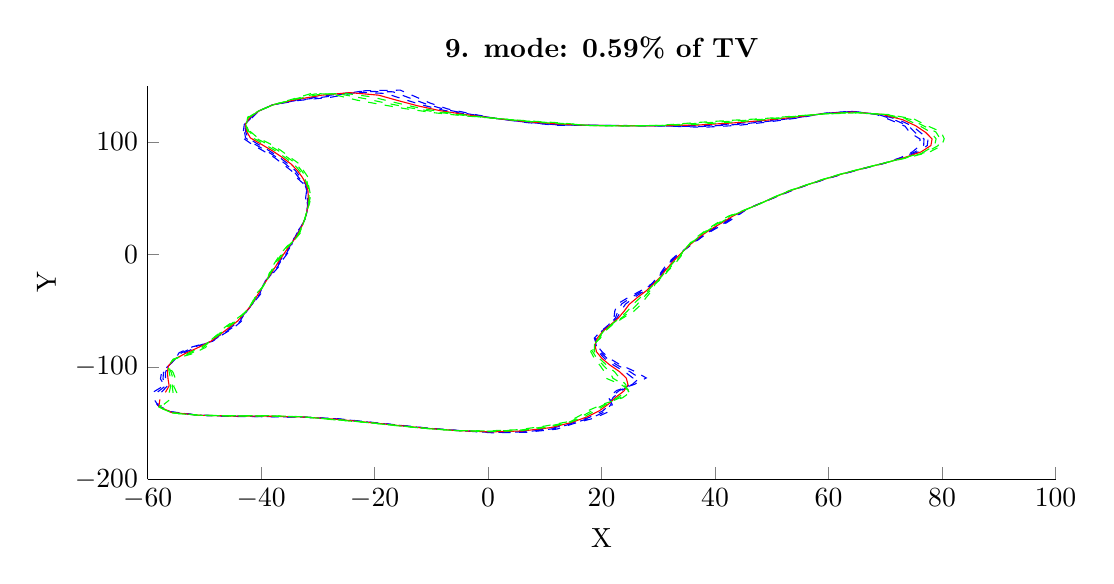
\begin{tikzpicture}

\begin{axis}[%
width=0.95092\figurewidth,
height=\figureheight,
at={(0\figurewidth,0\figureheight)},
scale only axis,
xmin=-60,
xmax=100,
xlabel={X},
ymin=-200,
ymax=150,
ylabel={Y},
title style={font=\bfseries},
title={9. mode: 0.59\% of TV},
axis x line*=bottom,
axis y line*=left
]
\addplot [color=blue,dashed,forget plot]
  table[row sep=crcr]{%
-58.8907821066333	-122.15062786793\\
-57.0240388355534	-116.484812996223\\
-57.7360125847147	-110.778764407841\\
-57.5505442335991	-105.110453143728\\
-56.3465004557491	-99.2446284228923\\
-55.1721571521483	-93.6657645296207\\
-54.4604020692611	-87.5385091439216\\
-52.0983661879419	-82.25261224849\\
-48.5564900906133	-77.3159291313996\\
-46.7878119986744	-71.4469924397915\\
-44.9119887625723	-65.6240831864899\\
-43.4913617748611	-59.6441939606333\\
-42.9444936084302	-53.4873734277665\\
-42.036065217939	-47.4028937411882\\
-41.060830467655	-41.3605959116097\\
-40.0824468015339	-35.2874889154235\\
-39.8270772868897	-29.205989868952\\
-39.1940479203893	-23.1945119664218\\
-37.9868059118704	-17.2624257857697\\
-36.9441917135059	-11.298722551564\\
-36.2405635897223	-5.20639003017042\\
-35.3608171429895	0.786390446256179\\
-34.7164873328981	6.78808016066841\\
-34.3150274841312	12.8399654961538\\
-33.7805772822007	18.9398033180454\\
-32.9187082934132	25.0683140952616\\
-32.2555269202657	31.2154905659576\\
-31.923736204557	37.3890933115162\\
-31.8573678904817	43.5596677815216\\
-32.1596104071358	49.7334792375704\\
-32.0007096801713	55.9126561022928\\
-32.3925149596838	62.0631382435085\\
-33.7041787099759	68.0735878478822\\
-34.6098382997285	74.0844361567833\\
-36.1215294750522	79.9984447153583\\
-37.6244844990743	85.9237905988038\\
-39.5429252064513	91.7397903650667\\
-41.5424503483306	97.4908734277592\\
-43.1518183679602	103.263211530833\\
-43.135931198182	109.358007018127\\
-42.9671295904553	115.3102198494\\
-41.6263615969647	121.147478737915\\
-40.4713500552167	127.148058506855\\
-38.0769764222166	132.713673357788\\
-33.4986605618067	136.698099517666\\
-27.6273497045561	139.668992856681\\
-21.5966505479445	145.483280276225\\
-15.4726979178419	145.922346014448\\
-12.8492738866471	140.188040486291\\
-10.2719329809913	134.550169152437\\
-7.10985820335891	129.209809882497\\
-2.78133479714448	124.689484017865\\
1.72201610640233	120.490046276677\\
6.77558989748006	117.128238072247\\
12.2774991903874	114.636225564005\\
18.5553158109897	114.71822207083\\
24.8039928176276	114.439558214001\\
31.369176245477	113.999684623472\\
37.970907194748	112.9093398302\\
44.1685939883688	114.652739827044\\
49.9119407956596	117.970909905299\\
55.2071668295127	121.644537894265\\
59.3968171052907	125.514732067641\\
64.1856813496063	127.232388087159\\
68.4529411715841	124.299386627441\\
71.0662634631066	119.07108006975\\
73.4884042334973	113.838554723606\\
74.3514087212218	108.013297673916\\
76.1116721037395	102.512615765345\\
76.1259661999358	96.7668403458117\\
74.8055936018198	91.1317231430175\\
72.5944691419484	85.7333294859371\\
69.6697584123328	80.6625158918921\\
66.0044856795766	76.0641309745758\\
62.4773944038257	71.2921499668877\\
59.2150657137325	66.3525225327583\\
56.066377746572	61.3201464836879\\
53.2495003145316	56.070714289775\\
50.6147856780122	50.7158712879194\\
47.9834375262517	45.3548697769149\\
45.5121988672649	39.8182650621298\\
43.8641402679954	33.8568924639271\\
41.993184325491	27.9619492040853\\
39.8724970859236	22.1457290388903\\
37.9535780747456	16.3108696136469\\
36.3493694168641	10.3764226384036\\
34.7311669409441	4.42407319926862\\
33.0138888063213	-1.56891194527036\\
31.6726482674077	-7.68392064595698\\
30.7719332251085	-13.916850198787\\
29.9219821094706	-20.1491490743456\\
28.80927327279	-26.3512347907557\\
26.9414758158628	-32.2931821656536\\
24.8021390959647	-38.0722734892519\\
22.8405103988408	-44.0362317831973\\
22.3368580283242	-50.26166885481\\
22.1936584235552	-56.5718112665051\\
21.2311247949543	-62.745867220127\\
19.8131017507686	-68.7552907637405\\
18.7177934340079	-74.463941243965\\
19.1147851054965	-80.6094173500942\\
20.106355047642	-86.7532268568907\\
21.3971996087516	-92.5111769037339\\
23.2693716923357	-98.1708703764726\\
25.8082904679611	-104.011660133564\\
27.8747291482788	-109.914309176647\\
25.7985479776948	-115.604469795589\\
22.6883435431965	-121.035128221635\\
21.2038547996481	-127.012478880791\\
21.8758732385449	-133.57606463114\\
21.3173196616493	-139.786676085521\\
18.8123630012509	-145.459226606243\\
15.0665847196582	-150.510239555064\\
12.0904500755809	-155.412145623383\\
6.87119574384553	-158.156543865205\\
0.952199153361228	-158.758730989075\\
-4.71511971287554	-156.847470827847\\
-10.3487380269169	-154.638921235539\\
-15.7401132616545	-151.840921985308\\
-21.0312674429255	-149.119791414274\\
-26.4286634632028	-146.166482827971\\
-32.5469312477137	-144.830422593801\\
-38.7735359230916	-144.434952541028\\
-44.9967220017007	-144.113949470106\\
-51.1588388749301	-143.019735579683\\
-56.03433827607	-139.841769134728\\
-58.1735613001845	-134.275416143129\\
-59.4550446848023	-128.141871705038\\
};
\addplot [color=blue,dashed,forget plot]
  table[row sep=crcr]{%
-58.2155497567055	-122.342092366055\\
-56.7520358514518	-116.635237276558\\
-57.2879544143866	-110.860691040949\\
-57.2082541594762	-105.112220910342\\
-56.346194987816	-99.2414180621319\\
-55.226273037665	-93.5987429802196\\
-54.0644739170295	-87.6807331220243\\
-51.7152829821643	-82.3560707444244\\
-48.6261374221788	-77.2213805002672\\
-46.9248687453728	-71.3593396515463\\
-45.1644380388642	-65.5217606280643\\
-43.7154256867052	-59.5808617987184\\
-42.9990621575558	-53.4848468013723\\
-42.0536731405494	-47.4341317088646\\
-41.126966165739	-41.4027792186087\\
-40.233609622915	-35.3448643310959\\
-39.8219947589914	-29.2793419456286\\
-39.152211956314	-23.2560048837134\\
-38.0902160436465	-17.2871057115441\\
-37.1278405771953	-11.2971122230894\\
-36.4162195702141	-5.1978080659532\\
-35.5454869384485	0.805859404746885\\
-34.8422619003175	6.82045578710204\\
-34.2756265290036	12.8635933622328\\
-33.6614706611475	18.9608550233532\\
-32.8821401843405	25.0981933634868\\
-32.265233518656	31.251688607518\\
-31.9347097125287	37.426932685263\\
-31.8079080810464	43.599917950016\\
-32.0017283299682	49.7766062486833\\
-31.9052907012909	55.9544723143645\\
-32.276051054869	62.111857707412\\
-33.3753539280612	68.1522221481928\\
-34.2670780486	74.169976379099\\
-35.6601274795375	80.1125455730039\\
-37.186237581045	86.0310137209683\\
-39.0418782814534	91.8539725669571\\
-41.0171193091218	97.5921019297738\\
-42.7342903208974	103.342052192605\\
-42.9482938080247	109.407428466186\\
-42.9017713766633	115.378760712181\\
-41.7496501527779	121.275806486549\\
-40.4491780134376	127.241037657437\\
-38.0108843215139	132.796055501639\\
-33.6102077375865	136.97435222797\\
-28.1899322697441	140.261438730859\\
-22.51366357483	144.888693009555\\
-16.7449369969407	144.440675032581\\
-13.8778475129949	139.036490230258\\
-10.9795048833876	133.691891914032\\
-7.51736902991857	128.652227061267\\
-3.03241963965589	124.425404208467\\
1.65463803755747	120.551855845886\\
6.7899141576295	117.385329614722\\
12.3282062155785	115.011423020046\\
18.4738565919758	114.664501824424\\
24.7018696475399	114.375030459143\\
31.2195023541624	114.114361819875\\
37.7310761840894	113.601060908412\\
43.8903100394871	115.381071655471\\
49.6737887629779	118.410414720627\\
55.0153188394784	121.859771071763\\
59.3534365382405	125.374227600816\\
64.2481436091753	126.976106552503\\
68.7946579972716	124.298002281715\\
71.7376098577984	119.25842775495\\
74.1271517347432	113.941055707025\\
75.266363167431	108.153119527914\\
76.8238553378655	102.541140976073\\
76.7635999351181	96.7346791473705\\
75.3000261957398	91.0831992816824\\
72.8313531898238	85.7714447651202\\
69.7173592866073	80.7775568141934\\
66.0305335663963	76.1449346456598\\
62.4688470205308	71.3726332624304\\
59.1828052176429	66.4090166247383\\
56.0455958760513	61.3326827853027\\
53.178314508045	56.0822622344431\\
50.5613153139524	50.6966103291475\\
47.9789406833366	45.2925925044458\\
45.4706847850334	39.7606094669628\\
43.6152710886978	33.8757246204362\\
41.7340179834822	27.9890118045226\\
39.6631170482259	22.1684214100414\\
37.8025831570517	16.3106061537603\\
36.2351822353185	10.3615364993329\\
34.7132682567662	4.38730994092615\\
33.1742549426524	-1.61773686897452\\
31.8947991695874	-7.73035077156656\\
30.9459243115162	-13.9462375003545\\
30.0687202441753	-20.1641185377636\\
28.9192050951116	-26.3454257514282\\
27.2541464501934	-32.3428808373703\\
25.3024778032604	-38.1920943236451\\
23.5181178795791	-44.1870871451319\\
22.8798090578131	-50.3849284551447\\
22.4424669425569	-56.6191926678347\\
21.3464733660524	-62.721654280116\\
19.9436180359884	-68.7021168640827\\
18.8966006801249	-74.4818670705907\\
19.0164532749964	-80.5988872029483\\
19.7729080021316	-86.7336541341906\\
20.9592509123143	-92.570749630798\\
22.6838094703709	-98.315004987368\\
24.935142508019	-104.148503962334\\
26.7013041577747	-109.97248755087\\
25.4180491955907	-115.673946529811\\
23.10809291059	-121.196140858869\\
21.6195071767871	-127.108754601645\\
21.6591159819524	-133.425878872339\\
20.7716891852547	-139.493448679003\\
18.3650378431409	-145.135038283673\\
14.9251163776037	-150.210002232673\\
11.7510768299254	-154.956013094974\\
6.62264531118211	-157.786607013885\\
0.772694670567678	-158.461347102138\\
-4.89868511030445	-156.82791092241\\
-10.4885735990603	-154.658954285607\\
-15.8483603590256	-151.909896694516\\
-21.1153969112243	-149.180405463636\\
-26.5373056990432	-146.327140924795\\
-32.5760922986002	-144.761464474271\\
-38.7806254276677	-144.264818243266\\
-45.0054168144941	-144.024216493603\\
-51.0806313855154	-143.039796355694\\
-55.943866188883	-140.09735001932\\
-58.124560083418	-134.623233005332\\
-58.9155176751163	-128.409745248602\\
};
\addplot [color=blue,dashed,forget plot]
  table[row sep=crcr]{%
-57.5403174067777	-122.53355686418\\
-56.4800328673501	-116.785661556893\\
-56.8398962440585	-110.942617674056\\
-56.8659640853533	-105.113988676955\\
-56.3458895198828	-99.2382077013715\\
-55.2803889231817	-93.5317214308185\\
-53.6685457647979	-87.822957100127\\
-51.3321997763866	-82.4595292403588\\
-48.6957847537442	-77.1268318691347\\
-47.0619254920712	-71.271686863301\\
-45.4168873151562	-65.4194380696386\\
-43.9394895985493	-59.5175296368034\\
-43.0536307066814	-53.4823201749781\\
-42.0712810631597	-47.465369676541\\
-41.1931018638231	-41.4449625256077\\
-40.3847724442962	-35.4022397467683\\
-39.8169122310931	-29.3526940223051\\
-39.1103759922387	-23.317497801005\\
-38.1936261754226	-17.3117856373185\\
-37.3114894408847	-11.2955018946149\\
-36.5918755507059	-5.18922610173597\\
-35.7301567339076	0.825328363237591\\
-34.9680364677369	6.85283141353568\\
-34.2362255738759	12.8872212283119\\
-33.5423640400944	18.9819067286609\\
-32.8455720752679	25.128072631712\\
-32.2749401170463	31.2878866490785\\
-31.9456832205003	37.4647720590099\\
-31.758448271611	43.6401681185104\\
-31.8438462528006	49.8197332597961\\
-31.8098717224106	55.9962885264362\\
-32.1595871500541	62.1605771713155\\
-33.0465291461464	68.2308564485035\\
-33.9243177974716	74.2555166014147\\
-35.1987254840227	80.2266464306496\\
-36.7479906630157	86.1382368431327\\
-38.5408313564554	91.9681547688476\\
-40.491788269913	97.6933304317884\\
-42.3167622738346	103.420892854377\\
-42.7606564178673	109.456849914246\\
-42.8364131628713	115.447301574963\\
-41.8729387085911	121.404134235183\\
-40.4270059716585	127.334016808019\\
-37.9447922208112	132.87843764549\\
-33.7217549133664	137.250604938273\\
-28.7525148349322	140.853884605036\\
-23.4306766017155	144.294105742884\\
-18.0171760760395	142.959004050714\\
-14.9064211393426	137.884939974225\\
-11.6870767857838	132.833614675626\\
-7.92487985647823	128.094644240036\\
-3.28350448216729	124.161324399068\\
1.5872599687126	120.613665415096\\
6.80423841777894	117.642421157197\\
12.3789132407696	115.386620476087\\
18.392397372962	114.610781578018\\
24.5997464774521	114.310502704286\\
31.0698284628478	114.229039016278\\
37.4912451734307	114.292781986624\\
43.6120260906053	116.109403483898\\
49.4356367302961	118.849919535955\\
54.8234708494441	122.07500424926\\
59.3100559711902	125.233723133991\\
64.3106058687443	126.719825017846\\
69.1363748229592	124.296617935989\\
72.4089562524901	119.445775440149\\
74.7658992359891	114.043556690444\\
76.1813176136401	108.292941381912\\
77.5360385719915	102.569666186802\\
77.4012336703004	96.7025179489294\\
75.7944587896598	91.0346754203473\\
73.0682372376993	85.8095600443033\\
69.7649601608818	80.8925977364947\\
66.0565814532159	76.2257383167438\\
62.460299637236	71.453116557973\\
59.1505447215534	66.4655107167184\\
56.0248140055305	61.3452190869175\\
53.1071287015584	56.0938101791112\\
50.5078449498927	50.6773493703756\\
47.9744438404214	45.2303152319767\\
45.429170702802	39.7029538717958\\
43.3664019094002	33.8945567769452\\
41.4748516414734	28.0160744049599\\
39.4537370105283	22.1911137811926\\
37.6515882393579	16.3103426938736\\
36.1209950537729	10.3466503602621\\
34.6953695725882	4.35054668258368\\
33.3346210789835	-1.66656179267868\\
32.116950071767	-7.77678089717615\\
31.1199153979238	-13.975624801922\\
30.21545837888	-20.1790880011816\\
29.0291369174332	-26.3396167121006\\
27.566817084524	-32.3925795090869\\
25.8028165105562	-38.3119151580384\\
24.1957253603174	-44.3379425070665\\
23.4227600873019	-50.5081880554794\\
22.6912754615586	-56.6665740691643\\
21.4618219371504	-62.6974413401051\\
20.0741343212081	-68.6489429644249\\
19.0754079262419	-74.4997928972164\\
18.9181214444963	-80.5883570558024\\
19.4394609566213	-86.7140814114905\\
20.521302215877	-92.630322357862\\
22.0982472484061	-98.4591395982634\\
24.0619945480769	-104.285347791103\\
25.5278791672706	-110.030665925093\\
25.0375504134866	-115.743423264034\\
23.5278422779835	-121.357153496102\\
22.0351595539261	-127.205030322499\\
21.4423587253599	-133.275693113538\\
20.2260587088601	-139.200221272485\\
17.9177126850309	-144.810849961103\\
14.7836480355491	-149.909764910282\\
11.4117035842699	-154.499880566565\\
6.3740948785187	-157.416670162565\\
0.593190187774128	-158.163963215201\\
-5.08225050773336	-156.808351016974\\
-10.6284091712037	-154.678987335674\\
-15.9566074563966	-151.978871403724\\
-21.1995263795231	-149.241019512998\\
-26.6459479348836	-146.487799021619\\
-32.6052533494867	-144.692506354742\\
-38.7877149322438	-144.094683945503\\
-45.0141116272875	-143.9344835171\\
-51.0024238961007	-143.059857131704\\
-55.853394101696	-140.352930903912\\
-58.0755588666514	-134.971049867534\\
-58.3759906654303	-128.677618792165\\
};
\addplot [color=red,solid,forget plot]
  table[row sep=crcr]{%
-56.8650850568499	-122.725021362305\\
-56.2080298832485	-116.936085837228\\
-56.3918380737305	-111.024544307164\\
-56.5236740112305	-105.115756443569\\
-56.3455840519496	-99.234997340611\\
-55.3345048086984	-93.4646998814174\\
-53.2726176125663	-87.9651810782296\\
-50.949116570609	-82.5629877362933\\
-48.7654320853097	-77.0322832380022\\
-47.1989822387695	-71.1840340750558\\
-45.6693365914481	-65.317115511213\\
-44.1635535103934	-59.4541974748884\\
-43.1081992558071	-53.479793548584\\
-42.0888889857701	-47.4966076442174\\
-41.2592375619071	-41.4871458326067\\
-40.5359352656773	-35.4596151624407\\
-39.8118297031948	-29.4260460989816\\
-39.0685400281634	-23.3789907182966\\
-38.2970363071987	-17.3364655630929\\
-37.4951383045741	-11.2938915661403\\
-36.7675315311977	-5.18064413751875\\
-35.9148265293666	0.844797321728298\\
-35.0938110351563	6.88520703996931\\
-34.1968246187483	12.9108490943909\\
-33.4232574190412	19.0029584339687\\
-32.8090039661952	25.1579518999372\\
-32.2846467154367	31.324084690639\\
-31.956656728472	37.5026114327567\\
-31.7089884621756	43.6804182870047\\
-31.685964175633	49.8628602709089\\
-31.7144527435303	56.038104738508\\
-32.0431232452393	62.209296635219\\
-32.7177043642317	68.3094907488142\\
-33.5815575463431	74.3410568237305\\
-34.737323488508	80.3407472882952\\
-36.3097437449864	86.2454599652972\\
-38.0397844314575	92.082336970738\\
-39.9664572307042	97.794558933803\\
-41.8992342267718	103.499733516148\\
-42.57301902771	109.506271362305\\
-42.7710549490792	115.515842437744\\
-41.9962272644043	121.532461983817\\
-40.4048339298793	127.426995958601\\
-37.8787001201085	132.960819789342\\
-33.8333020891462	137.526857648577\\
-29.3150974001203	141.446330479213\\
-24.3476896286011	143.699518476214\\
-19.2894151551383	141.477333068848\\
-15.9349947656904	136.733389718192\\
-12.3946486881801	131.975337437221\\
-8.33239068303789	127.537061418806\\
-3.53458932467869	123.897244589669\\
1.51988189986774	120.675474984305\\
6.81856267792838	117.899512699672\\
12.4296202659607	115.761817932129\\
18.3109381539481	114.557061331613\\
24.4976233073643	114.245974949428\\
30.9201545715332	114.343716212681\\
37.251414162772	114.984503064837\\
43.3337421417236	116.837735312326\\
49.1974846976144	119.289424351283\\
54.6316228594099	122.290237426758\\
59.2666754041399	125.093218667167\\
64.3730681283133	126.463543483189\\
69.4780916486468	124.295233590262\\
73.0803026471819	119.633123125349\\
75.4046467372349	114.146057673863\\
77.0962720598493	108.43276323591\\
78.2482218061175	102.598191397531\\
78.0388674054827	96.6703567504883\\
76.2888913835798	90.9861515590123\\
73.3051212855748	85.8476753234863\\
69.8125610351563	81.007638658796\\
66.0826293400356	76.3065419878278\\
62.4517522539411	71.5335998535156\\
59.1182842254639	66.5220048086984\\
56.0040321350098	61.3577553885324\\
53.0359428950718	56.1053581237793\\
50.4543745858329	50.6580884116037\\
47.9699469975063	45.1680379595075\\
45.3876566205706	39.6452982766288\\
43.1175327301025	33.9133889334542\\
41.2156852994646	28.0431370053973\\
39.2443569728306	22.2138061523438\\
37.500593321664	16.310079233987\\
36.0068078722273	10.3317642211914\\
34.6774708884103	4.3137834242412\\
33.4949872153146	-1.71538671638284\\
32.3391009739467	-7.82321102278573\\
31.2939064843314	-14.0050121034895\\
30.3621965135847	-20.1940574645996\\
29.1390687397548	-26.3338076727731\\
27.8794877188546	-32.4422781808036\\
26.3031552178519	-38.4317359924316\\
24.8733328410557	-44.4887978690011\\
23.9657111167908	-50.631447655814\\
22.9400839805603	-56.7139554704939\\
21.5771705082485	-62.6732284000942\\
20.2046506064279	-68.595769064767\\
19.2542151723589	-74.5177187238421\\
18.8197896139962	-80.5778269086565\\
19.106013911111	-86.6945086887905\\
20.0833535194397	-92.6898950849261\\
21.5126850264413	-98.6032742091588\\
23.1888465881348	-104.422191619873\\
24.3544541767665	-110.088844299316\\
24.6570516313825	-115.812899998256\\
23.947591645377	-121.518166133336\\
22.4508119310652	-127.301306043352\\
21.2256014687674	-133.125507354736\\
19.6804282324655	-138.906993865967\\
17.4703875269209	-144.486661638532\\
14.6421796934945	-149.609527587891\\
11.0723303386143	-154.043748038156\\
6.12554444585528	-157.046733311244\\
0.413685704980578	-157.866579328265\\
-5.26581590516227	-156.788791111537\\
-10.7682447433472	-154.699020385742\\
-16.0648545537676	-152.047846112932\\
-21.2836558478219	-149.30163356236\\
-26.7545901707241	-146.648457118443\\
-32.6344144003732	-144.623548235212\\
-38.7948044368199	-143.92454964774\\
-45.0228064400809	-143.844750540597\\
-50.924216406686	-143.079917907715\\
-55.7629220145089	-140.608511788504\\
-58.0265576498849	-135.318866729736\\
-57.8364636557443	-128.945492335728\\
};
\addplot [color=green,dashed,forget plot]
  table[row sep=crcr]{%
-56.1898527069221	-122.91648586043\\
-55.9360268991468	-117.086510117563\\
-55.9437799034024	-111.106470940271\\
-56.1813839371076	-105.117524210182\\
-56.3452785840165	-99.2317869798506\\
-55.3886206942151	-93.3976783320163\\
-52.8766894603346	-88.1074050563323\\
-50.5660333648313	-82.6664462322277\\
-48.8350794168752	-76.9377346068698\\
-47.3360389854679	-71.0963812868106\\
-45.92178586774	-65.2147929527874\\
-44.3876174222375	-59.3908653129734\\
-43.1627678049327	-53.4772669221898\\
-42.1064969083804	-47.5278456118937\\
-41.3253732599911	-41.5293291396057\\
-40.6870980870585	-35.5169905781131\\
-39.8067471752964	-29.4993981756581\\
-39.026704064088	-23.4404836355882\\
-38.4004464389748	-17.3611454888673\\
-37.6787871682636	-11.2922812376658\\
-36.9431875116895	-5.17206217330152\\
-36.0994963248257	0.864266280219004\\
-35.2195856025756	6.91758266640294\\
-34.1574236636206	12.9344769604699\\
-33.3041507979881	19.0240101392764\\
-32.7724358571226	25.1878311681624\\
-32.294353313827	31.3602827321994\\
-31.9676302364437	37.5404508065035\\
-31.6595286527403	43.7206684554991\\
-31.5280820984654	49.9059872820217\\
-31.6190337646499	56.0799209505797\\
-31.9266593404244	62.2580160991225\\
-32.3888795823169	68.3881250491248\\
-33.2387972952147	74.4265970460462\\
-34.2759214929932	80.4548481459408\\
-35.8714968269571	86.3526830874616\\
-37.5387375064596	92.1965191726284\\
-39.4411261914954	97.8957874358176\\
-41.4817061797089	103.57857417792\\
-42.3853816375526	109.555692810364\\
-42.7056967352872	115.584383300526\\
-42.1195158202175	121.660789732451\\
-40.3826618881002	127.519975109183\\
-37.8126080194058	133.043201933193\\
-33.9448492649261	137.803110358881\\
-29.8776799653084	142.03877635339\\
-25.2647026554866	143.104931209543\\
-20.5616542342371	139.995662086981\\
-16.9635683920382	135.581839462159\\
-13.1022205905764	131.117060198816\\
-8.73990150959756	126.979478597575\\
-3.7856741671901	123.633164780271\\
1.45250383102287	120.737284553515\\
6.83288693807782	118.156604242147\\
12.4803272911518	116.13701538817\\
18.2294789349342	114.503341085207\\
24.3955001372766	114.18144719457\\
30.7704806802186	114.458393409084\\
37.0115831521134	115.676224143049\\
43.0554581928419	117.566067140753\\
48.9593326649327	119.728929166612\\
54.4397748693756	122.505470604255\\
59.2232948370897	124.952714200342\\
64.4355303878824	126.207261948532\\
69.8198084743343	124.293849244536\\
73.7516490418737	119.820470810548\\
76.0433942384808	114.248558657282\\
78.0112265060585	108.572585089907\\
78.9604050402435	102.626716608259\\
78.676501140665	96.6381955520472\\
76.7833239774998	90.9376276976772\\
73.5420053334502	85.8857906026694\\
69.8601619094307	81.1226795810974\\
66.1086772268552	76.3873456589118\\
62.4432048706463	71.6140831490583\\
59.0860237293743	66.5784989006784\\
55.983250264489	61.3702916901472\\
52.9647570885853	56.1169060684474\\
50.4009042217731	50.6388274528317\\
47.9654501545911	45.1057606870384\\
45.3461425383392	39.5876426814617\\
42.8686635508049	33.9322210899633\\
40.9565189574558	28.0701996058346\\
39.034976935133	22.2364985234949\\
37.3495984039701	16.3098157741004\\
35.8926206906816	10.3168780821207\\
34.6595722042324	4.27702016589873\\
33.6553533516457	-1.76421164008701\\
32.5612518761264	-7.86964114839532\\
31.467897570739	-14.0343994050569\\
30.5089346482894	-20.2090269280176\\
29.2490005620764	-26.3279986334456\\
28.1921583531852	-32.4919768525202\\
26.8034939251477	-38.5515568268249\\
25.5509403217941	-44.6396532309357\\
24.5086621462796	-50.7547072561487\\
23.188892499562	-56.7613368718235\\
21.6925190793465	-62.6490154600832\\
20.3351668916476	-68.5425951651092\\
19.4330224184759	-74.5356445504678\\
18.7214577834962	-80.5672967615107\\
18.7725668656007	-86.6749359660904\\
19.6454048230024	-92.7494678119901\\
20.9271228044765	-98.7474088200541\\
22.3156986281926	-104.559035448643\\
23.1810291862625	-110.14702267354\\
24.2765528492784	-115.882376732479\\
24.3673410127705	-121.679178770569\\
22.8664643082042	-127.397581764206\\
21.008844212175	-132.975321595935\\
19.1347977560709	-138.613766459449\\
17.0230623688109	-144.162473315962\\
14.50071135144	-149.309290265499\\
10.7329570929588	-153.587615509746\\
5.87699401319186	-156.676796459924\\
0.234181222187028	-157.569195441328\\
-5.44938130259118	-156.769231206101\\
-10.9080803154906	-154.71905343581\\
-16.1731016511386	-152.116820822141\\
-21.3677853161207	-149.362247611723\\
-26.8632324065645	-146.809115215267\\
-32.6635754512597	-144.554590115682\\
-38.801893941396	-143.754415349977\\
-45.0315012528743	-143.755017564094\\
-50.8460089172712	-143.099978683725\\
-55.6724499273219	-140.864092673097\\
-57.9775564331184	-135.666683591939\\
-57.2969366460583	-129.213365879292\\
};
\addplot [color=green,dashed,forget plot]
  table[row sep=crcr]{%
-55.5146203569943	-123.107950358555\\
-55.6640239150452	-117.236934397898\\
-55.4957217330743	-111.188397573379\\
-55.8390938629847	-105.119291976796\\
-56.3449731160833	-99.2285766190902\\
-55.4427365797318	-93.3306567826152\\
-52.480761308103	-88.249629034435\\
-50.1829501590537	-82.7699047281621\\
-48.9047267484407	-76.8431859757373\\
-47.4730957321663	-71.0087284985653\\
-46.174235144032	-65.1124703943618\\
-44.6116813340816	-59.3275331510584\\
-43.2173363540583	-53.4747402957957\\
-42.1241048309908	-47.5590835795701\\
-41.3915089580751	-41.5715124466048\\
-40.8382609084396	-35.5743659937855\\
-39.8016646473981	-29.5727502523346\\
-38.9848681000127	-23.5019765528798\\
-38.5038565707509	-17.3858254146417\\
-37.862436031953	-11.2906709091912\\
-37.1188434921813	-5.1634802090843\\
-36.2841661202847	0.88373523870971\\
-35.345360169995	6.94995829283657\\
-34.118022708493	12.9581048265489\\
-33.1850441769349	19.0450618445842\\
-32.7358677480499	25.2177104363876\\
-32.3040599122173	31.3964807737599\\
-31.9786037444154	37.5782901802503\\
-31.6100688433049	43.7609186239935\\
-31.3702000212979	49.9491142931345\\
-31.5236147857696	56.1217371626514\\
-31.8101954356095	62.306735563026\\
-32.0600548004022	68.4667593494355\\
-32.8960370440862	74.5121372683619\\
-33.8145194974784	80.5689490035865\\
-35.4332499089278	86.4599062096261\\
-37.0376905814617	92.3107013745189\\
-38.9157951522865	97.9970159378322\\
-41.0641781326461	103.657414839691\\
-42.1977442473952	109.605114258423\\
-42.6403385214952	115.652924163307\\
-42.2428043760307	121.789117481085\\
-40.3604898463211	127.612954259764\\
-37.746515918703	133.125584077044\\
-34.0563964407059	138.079363069184\\
-30.4402625304965	142.631222227568\\
-26.1817156823722	142.510343942873\\
-21.8338933133359	138.513991105114\\
-17.9921420183859	134.430289206126\\
-13.8097924929726	130.25878296041\\
-9.14741233615722	126.421895776345\\
-4.0367590097015	123.369084970872\\
1.38512576217801	120.799094122724\\
6.84721119822726	118.413695784622\\
12.5310343163429	116.512212844212\\
18.1480197159204	114.449620838801\\
24.2933769671888	114.116919439713\\
30.620806788904	114.573070605487\\
36.7717521414547	116.367945221261\\
42.7771742439602	118.29439896918\\
48.7211806322509	120.16843398194\\
54.2479268793414	122.720703781753\\
59.1799142700394	124.812209733517\\
64.4979926474514	125.950980413876\\
70.1615253000219	124.29246489881\\
74.4229954365655	120.007818495748\\
76.6821417397266	114.351059640701\\
78.9261809522677	108.712406943905\\
79.6725882743695	102.655241818988\\
79.3141348758473	96.606034353606\\
77.2777565714198	90.8891038363422\\
73.7788893813257	85.9239058818525\\
69.9077627837052	81.2377205033987\\
66.1347251136749	76.4681493299958\\
62.4346574873514	71.6945664446009\\
59.0537632332848	66.6349929926585\\
55.9624683939683	61.382827991762\\
52.8935712820987	56.1284540131155\\
50.3474338577133	50.6195664940598\\
47.960953311676	45.0434834145693\\
45.3046284561078	39.5299870862947\\
42.6197943715073	33.9510532464723\\
40.697352615447	28.0972622062719\\
38.8255968974353	22.2591908946461\\
37.1986034862763	16.3095523142137\\
35.778433509136	10.30199194305\\
34.6416735200544	4.24025690755626\\
33.8157194879768	-1.81303656379117\\
32.7834027783061	-7.9160712740049\\
31.6418886571467	-14.0637867066244\\
30.6556727829941	-20.2239963914356\\
29.358932384398	-26.322189594118\\
28.5048289875159	-32.5416755242369\\
27.3038326324434	-38.6713776612182\\
26.2285478025324	-44.7905085928703\\
25.0516131757685	-50.8779668564834\\
23.4377010185637	-56.8087182731531\\
21.8078676504445	-62.6248025200723\\
20.4656831768674	-68.4894212654514\\
19.6118296645929	-74.5535703770935\\
18.6231259529961	-80.5567666143648\\
18.4391198200904	-86.6553632433903\\
19.2074561265651	-92.8090405390542\\
20.3415605825117	-98.8915434309495\\
21.4425506682505	-104.695879277412\\
22.0076041957584	-110.205201047763\\
23.8960540671743	-115.951853466701\\
24.787090380164	-121.840191407803\\
23.2821166853432	-127.49385748506\\
20.7920869555825	-132.825135837134\\
18.5891672796763	-138.32053905293\\
16.5757372107009	-143.838284993392\\
14.3592430093854	-149.009052943108\\
10.3935838473033	-153.131482981337\\
5.62844358052844	-156.306859608604\\
0.0546767393934775	-157.271811554391\\
-5.63294670002008	-156.749671300665\\
-11.047915887634	-154.739086485878\\
-16.2813487485097	-152.185795531349\\
-21.4519147844195	-149.422861661085\\
-26.9718746424049	-146.969773312091\\
-32.6927365021462	-144.485631996153\\
-38.8089834459721	-143.584281052214\\
-45.0401960656677	-143.665284587591\\
-50.7678014278565	-143.120039459736\\
-55.5819778401349	-141.119673557689\\
-57.9285552163518	-136.014500454141\\
-56.7574096363723	-129.481239422855\\
};
\addplot [color=green,dashed,forget plot]
  table[row sep=crcr]{%
-54.8393880070664	-123.29941485668\\
-55.3920209309435	-117.387358678233\\
-55.0476635627463	-111.270324206486\\
-55.4968037888618	-105.121059743409\\
-56.3446676481502	-99.2253662583298\\
-55.4968524652485	-93.2636352332141\\
-52.0848331558714	-88.3918530125377\\
-49.799866953276	-82.8733632240966\\
-48.9743740800062	-76.7486373446048\\
-47.6101524788646	-70.9210757103201\\
-46.4266844203239	-65.0101478359362\\
-44.8357452459258	-59.2642009891434\\
-43.2719049031839	-53.4722136694015\\
-42.1417127536011	-47.5903215472465\\
-41.4576446561591	-41.6136957536038\\
-40.9894237298208	-35.6317414094579\\
-39.7965821194998	-29.6461023290111\\
-38.9430321359374	-23.5634694701714\\
-38.607266702527	-17.4105053404161\\
-38.0460848956424	-11.2890605807166\\
-37.2944994726731	-5.15489824486707\\
-36.4688359157438	0.903204197200416\\
-35.4711347374144	6.9823339192702\\
-34.0786217533653	12.9817326926279\\
-33.0659375558818	19.0661135498919\\
-32.6992996389773	25.2475897046128\\
-32.3137665106076	31.4326788153203\\
-31.9895772523871	37.6161295539972\\
-31.5606090338696	43.8011687924879\\
-31.2123179441303	49.9922413042474\\
-31.4281958068893	56.1635533747231\\
-31.6937315307947	62.3554550269295\\
-31.7312300184874	68.5453936497462\\
-32.5532767929578	74.5976774906776\\
-33.3531175019637	80.6830498612321\\
-34.9950029908985	86.5671293317905\\
-36.5366436564638	92.4248835764093\\
-38.3904641130777	98.0982444398468\\
-40.6466500855833	103.736255501463\\
-42.0101068572379	109.654535706482\\
-42.5749803077032	115.721465026089\\
-42.3660929318439	121.917445229718\\
-40.3383178045419	127.705933410346\\
-37.6804238180003	133.207966220895\\
-34.1679436164858	138.355615779488\\
-31.0028450956846	143.223668101745\\
-27.0987287092577	141.915756676202\\
-23.1061323924347	137.032320123247\\
-19.0207156447337	133.278738950093\\
-14.5173643953689	129.400505722005\\
-9.55492316271688	125.864312955114\\
-4.28784385221291	123.105005161473\\
1.31774769333314	120.860903691933\\
6.8615354583767	118.670787327097\\
12.581741341534	116.887410300253\\
18.0665604969065	114.395900592396\\
24.191253797101	114.052391684855\\
30.4711328975894	114.68774780189\\
36.5319211307961	117.059666299474\\
42.4988902950785	119.022730797607\\
48.4830285995692	120.607938797268\\
54.0560788893071	122.935936959251\\
59.1365337029891	124.671705266692\\
64.5604549070204	125.694698879219\\
70.5032421257094	124.291080553083\\
75.0943418312573	120.195166180947\\
77.3208892409725	114.45356062412\\
79.8411353984769	108.852228797903\\
80.3847715084955	102.683767029717\\
79.9517686110296	96.5738731551649\\
77.7721891653398	90.8405799750071\\
74.0157734292012	85.9620211610356\\
69.9553636579797	81.3527614257\\
66.1607730004946	76.5489530010798\\
62.4261101040566	71.7750497401435\\
59.0215027371953	66.6914870846385\\
55.9416865234475	61.3953642933769\\
52.8223854756121	56.1400019577836\\
50.2939634936535	50.6003055352879\\
47.9564564687608	44.9812061421002\\
45.2631143738763	39.4723314911277\\
42.3709251922097	33.9698854029814\\
40.4381862734382	28.1243248067093\\
38.6162168597377	22.2818832657972\\
37.0476085685824	16.3092888543271\\
35.6642463275904	10.2871058039792\\
34.6237748358765	4.20349364921378\\
33.9760856243079	-1.86186148749533\\
33.0055536804857	-7.96250139961449\\
31.8158797435543	-14.0931740081919\\
30.8024109176988	-20.2389658548536\\
29.4688642067196	-26.3163805547905\\
28.8174996218465	-32.5913741959535\\
27.8041713397392	-38.7911984956114\\
26.9061552832707	-44.941363954805\\
25.5945642052573	-51.0012264568181\\
23.6865095375654	-56.8560996744827\\
21.9232162215426	-62.6005895800614\\
20.5961994620871	-68.4362473657935\\
19.7906369107099	-74.5714962037192\\
18.524794122496	-80.5462364672189\\
18.1056727745801	-86.6357905206902\\
18.7695074301278	-92.8686132661182\\
19.7559983605469	-99.0356780418449\\
20.5694027083084	-104.832723106182\\
20.8341792052543	-110.263379421986\\
23.5155552850702	-116.021330200924\\
25.2068397475575	-122.001204045036\\
23.6977690624822	-127.590133205914\\
20.57532969899	-132.674950078333\\
18.0435368032817	-138.027311646412\\
16.1284120525908	-143.514096670822\\
14.2177746673308	-148.708815620717\\
10.0542106016477	-152.675350452928\\
5.37989314786502	-155.936922757284\\
-0.124827743400073	-156.974427667454\\
-5.81651209744899	-156.730111395228\\
-11.1877514597775	-154.759119535946\\
-16.3895958458807	-152.254770240557\\
-21.5360442527183	-149.483475710447\\
-27.0805168782453	-147.130431408915\\
-32.7218975530327	-144.416673876623\\
-38.8160729505482	-143.414146754452\\
-45.0488908784611	-143.575551611088\\
-50.6895939384418	-143.140100235746\\
-55.4915057529479	-141.375254442281\\
-57.8795539995853	-136.362317316343\\
-56.2178826266863	-129.749112966418\\
};
\end{axis}
\end{tikzpicture}%
					\caption{Modus 9}
					\label{fig:mode9}
				\end{subfigure}	
				\\
				\begin{subfigure}{0.3\textwidth}
					\centering
					% This file was created by matlab2tikz.
% Minimal pgfplots version: 1.3
%
%The latest updates can be retrieved from
%  http://www.mathworks.com/matlabcentral/fileexchange/22022-matlab2tikz
%where you can also make suggestions and rate matlab2tikz.
%
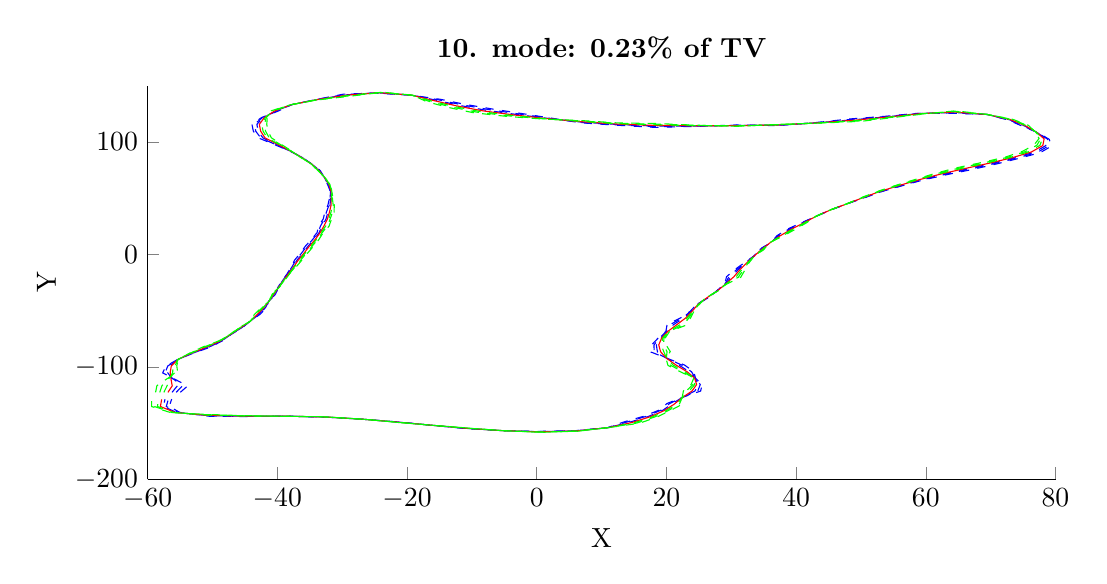
\begin{tikzpicture}

\begin{axis}[%
width=0.95092\figurewidth,
height=\figureheight,
at={(0\figurewidth,0\figureheight)},
scale only axis,
xmin=-60,
xmax=80,
xlabel={X},
ymin=-200,
ymax=150,
ylabel={Y},
title style={font=\bfseries},
title={10. mode: 0.23\% of TV},
axis x line*=bottom,
axis y line*=left
]
\addplot [color=blue,dashed,forget plot]
  table[row sep=crcr]{%
-54.9595165742425	-122.692675608428\\
-53.8431054453685	-117.071450205754\\
-55.7402406266517	-111.237599251278\\
-57.6787660967231	-105.442750157743\\
-57.1849809992114	-99.4541997211813\\
-55.4490707201289	-93.7478176488856\\
-53.0818271565141	-88.2080809380401\\
-50.4086252288837	-82.7158725081058\\
-48.4762498919583	-76.9701497364713\\
-47.0865955821023	-71.0782759182934\\
-45.3984150548802	-65.254593770005\\
-44.1532419812208	-59.3053842486984\\
-42.6668791749438	-53.415601629134\\
-41.694320099724	-47.4417832944741\\
-41.2991549054838	-41.411492380985\\
-40.1472788127517	-35.4586706145675\\
-39.9150018447772	-29.39762974492\\
-39.2315691172629	-23.3113661809741\\
-38.482109575537	-17.2508064284697\\
-37.8540896452297	-11.1655260537728\\
-37.3152619391575	-5.05566579971978\\
-36.4500554029661	0.975374118711146\\
-35.7016007055481	7.0318091393465\\
-34.759409281345	13.0633871683217\\
-33.883568154649	19.1276179114182\\
-33.6006729512097	25.2832266818236\\
-32.9227020684139	31.392509371977\\
-32.6629660579235	37.5359610635655\\
-32.2024375663507	43.6817179738343\\
-31.9570876973736	49.837967534502\\
-31.8301055705519	56.008131402074\\
-32.2594328375757	62.1493035771963\\
-32.7619264623363	68.3134484735943\\
-33.3842608340568	74.502009803784\\
-34.7355244822345	80.4860409643874\\
-36.2026234827257	86.4205247218874\\
-38.2349086868372	92.1292541758684\\
-40.5042737693393	97.6990252805103\\
-42.8699909444254	103.364422524147\\
-43.6970820716382	109.398805515984\\
-43.9118164109502	115.510100592724\\
-42.4432872905667	121.524972719229\\
-39.8814132258389	127.281989046802\\
-37.7487970340401	133.072089073193\\
-33.7916248695654	137.84528375825\\
-29.8155053233359	142.349701865762\\
-24.9405490120864	143.32463697005\\
-19.4655351519885	141.503154748933\\
-14.904738428745	137.836015540179\\
-11.1818795042717	133.413601120838\\
-6.84918372103579	129.16795873683\\
-2.31448872741329	125.128958348977\\
2.25149667092361	121.027926581176\\
6.7991539696838	116.88652989438\\
12.419871634607	114.735381369302\\
18.2156570524833	112.836919013712\\
24.4289470163542	113.728901809264\\
30.7881740168927	114.908676895438\\
37.0656563188027	114.441868292082\\
42.856503285541	116.993765920609\\
48.3529249861154	120.345143852032\\
53.9894131504591	122.775528814021\\
58.6211560076846	125.30850697934\\
64.1646237165479	125.392974496931\\
69.4293890958191	124.302066358242\\
72.7454086318429	119.296655373885\\
74.9869395790507	113.64214417906\\
77.3254290958776	108.028586359665\\
79.0307137271525	102.218508175779\\
79.3890389433898	96.2128813731844\\
77.6445044465878	90.3797428554856\\
74.3378337603846	85.259261288604\\
70.899734906142	80.3265285329992\\
67.2434582628167	75.4996606492123\\
63.3218555369701	70.9161858013765\\
59.6311272052207	66.1346574095717\\
56.4022821940693	61.0249764932842\\
53.2647911380654	55.8636893992342\\
50.6271639636176	50.4514698594775\\
47.9466224219876	45.0615053378601\\
45.3819336766542	39.5499565222673\\
43.0989805722864	33.8289252392094\\
40.8355723480959	28.1005422544355\\
38.66425425217	22.3811517243322\\
37.0311885266092	16.468204741019\\
36.1475259014304	10.356479953123\\
34.3301412993571	4.46281615109716\\
33.4815972521032	-1.64640621032296\\
31.9911359059181	-7.65994541301353\\
30.5074072306373	-13.7434738278709\\
29.2754395730137	-19.900766756544\\
29.005567732222	-26.1750678875899\\
27.7920531324416	-32.3227918567296\\
26.5555908314742	-38.381255498455\\
24.6752478322777	-44.3755708429518\\
23.6943665435501	-50.5944487652141\\
22.1805656561714	-56.5700863436846\\
20.1103614623823	-62.3380168125608\\
19.9138947400833	-68.6088504584587\\
18.7038167806054	-74.5877211163513\\
17.707865469378	-80.688425796048\\
17.6232739309079	-86.9212318877984\\
20.2227562653032	-92.7289757997772\\
22.7838779566191	-98.4207809029337\\
24.2098668672787	-104.33062504434\\
24.4940120826084	-110.138203290501\\
25.5044771593712	-115.837750262431\\
25.2736033554947	-121.595175290895\\
22.4802227332848	-127.09740710389\\
20.0919882932489	-132.650365646508\\
18.9031514383363	-138.471945045691\\
16.5004516296684	-144.021875643276\\
13.4597682928691	-149.024725151207\\
10.9559204783409	-154.099732053459\\
5.94413139867505	-156.800289940527\\
0.295703755884649	-157.439089031907\\
-5.30529422309284	-156.824194914354\\
-10.8676263948378	-154.955800975287\\
-16.0205124303603	-152.112401263143\\
-21.1018809595712	-149.154306626916\\
-26.6320096959408	-146.74747892951\\
-32.4601830203341	-144.810430154155\\
-38.5141619910492	-143.875327736802\\
-44.6996236250702	-144.224981589871\\
-50.4820342960702	-143.941983032981\\
-55.0362134787143	-140.555607004756\\
-56.6647382433822	-135.293867495136\\
-56.2871912626088	-128.748014113179\\
};
\addplot [color=blue,dashed,forget plot]
  table[row sep=crcr]{%
-55.5947060684449	-122.703457526387\\
-54.6314135913285	-117.026328749579\\
-55.957439775678	-111.166580936573\\
-57.2937354015589	-105.333752253018\\
-56.9051820167908	-99.3811322609912\\
-55.4108820829854	-93.6534450597295\\
-53.1454239751982	-88.1271143181033\\
-50.5887890094588	-82.6649109175017\\
-48.5726439564088	-76.9908609036483\\
-47.1240578009914	-71.1135286372142\\
-45.4887222337362	-65.2754343504077\\
-44.1566791576117	-59.3549886574284\\
-42.8139858685649	-53.4369989356173\\
-41.8258430617394	-47.4600580777219\\
-41.2858491242916	-41.4367101981922\\
-40.2768309637269	-35.4589854638586\\
-39.8806111309164	-29.4071018629405\\
-39.1772260875631	-23.3339076934149\\
-38.4204184860909	-17.2793594733441\\
-37.7344391983445	-11.2083145578953\\
-37.1326851365042	-5.09732524565277\\
-36.2716457784329	0.931848519716863\\
-35.4990041487508	6.98294177288744\\
-34.5718810604794	13.0125411436781\\
-33.7301312427798	19.0860647522684\\
-33.3367832895382	25.2414684211948\\
-32.7100169507548	31.3697011448643\\
-32.427529614773	37.5248445199626\\
-32.0379545316257	43.6812847448911\\
-31.8667131901267	49.8462651133043\\
-31.7915546282114	56.0181225142186\\
-32.1873296401302	62.1693012632039\\
-32.7471857629681	68.3121292320009\\
-33.4500264048189	74.4483588104328\\
-34.7361241509923	80.4376097390233\\
-36.2383302368126	86.362169803024\\
-38.1698672683773	92.1136151074916\\
-40.3250015897943	97.7308698316079\\
-42.5464053718742	103.409526188147\\
-43.3223943903288	109.434627464757\\
-43.5315625903266	115.512014541064\\
-42.2942672818459	121.527469140758\\
-40.0558867938524	127.330324684068\\
-37.7920980627296	133.034999311909\\
-33.8055172760923	137.739141721692\\
-29.648702682264	142.048578070246\\
-24.7429292175913	143.449597472105\\
-19.4068284863718	141.494547522238\\
-15.2481572077268	137.468473599517\\
-11.5861358989079	132.934179892966\\
-7.34358604170316	128.624326297488\\
-2.72118892650176	124.718387095874\\
2.00762508057165	120.910442715553\\
6.80562353909866	117.224190829477\\
12.4231211783916	115.077526890244\\
18.2474174196382	113.410299786346\\
24.4518391133576	113.901259522652\\
30.8321675351062	114.720356667852\\
37.1275756001258	114.622746549667\\
43.0155829042686	116.941755717848\\
48.6344448899484	119.993237351783\\
54.2034830534427	122.613765018267\\
58.8363291398364	125.236744208616\\
64.2341051871363	125.749830825684\\
69.445623280095	124.299788768916\\
72.8570399702892	119.408811291039\\
75.1261752984455	113.810115343995\\
77.2490434172015	108.16331198508\\
78.7698830868075	102.345069249696\\
78.9389817640875	96.3653731656191\\
77.1926334255851	90.5818790899945\\
73.9935962687813	85.4553993002314\\
70.5373436158134	80.5535652415982\\
66.8565152885563	75.7686210954175\\
63.0318211092938	71.1219904854229\\
59.4601795453017	66.2637732092806\\
56.2695321743828	61.1359027917003\\
53.1885083904009	55.9442456407492\\
50.569567504356	50.5203427101862\\
47.9543972804939	45.0970162117426\\
45.3838413246264	39.5817371070545\\
43.1051646248918	33.8570798039577\\
40.9622766652188	28.0814071714228\\
38.8576218257235	22.3253698670027\\
37.1876567916275	16.415496238675\\
36.1006198916961	10.3482413758125\\
34.4459178290415	4.41313857547851\\
33.4860605731736	-1.66939971234292\\
32.1071242619276	-7.7143672829376\\
30.7695736485354	-13.8306532530771\\
29.6376918865374	-19.9985303258959\\
29.0500680680663	-26.2279811493176\\
27.8211979945793	-32.3626206314209\\
26.4714456269334	-38.3980823297805\\
24.741276168537	-44.4133131849683\\
23.7848147346303	-50.6067817287474\\
22.4337384309677	-56.6180427192877\\
20.5992978110043	-62.4497540084053\\
20.0108133621981	-68.6044899938948\\
18.8872829111899	-74.5643869855149\\
18.0785068509174	-80.6515595002508\\
18.1175205909756	-86.8456574881291\\
20.1762886833487	-92.7159488948268\\
22.3601469798932	-98.4816120050088\\
23.8695267742307	-104.361147236184\\
24.4474927806611	-110.12175029344\\
25.222001983375	-115.829466841039\\
24.8315994521222	-121.569505571709\\
22.4704191325449	-127.165373417044\\
20.4698593517551	-132.808746215918\\
19.1622437030461	-138.616961319116\\
16.8237635954192	-144.176804308361\\
13.8539054264109	-149.219659296768\\
10.9947237650987	-154.081070715025\\
6.00460241440179	-156.882437730766\\
0.335031072249958	-157.581585797359\\
-5.29213478378265	-156.812393646749\\
-10.8344991776742	-154.870207445439\\
-16.0352931381627	-152.09088287974\\
-21.1624725889881	-149.203415605397\\
-26.6728698542019	-146.714471659154\\
-32.5182601470138	-144.748136181174\\
-38.6077094729728	-143.891735040448\\
-44.8073512300738	-144.098237906779\\
-50.6294283329421	-143.654627991226\\
-55.2784496573125	-140.573241932672\\
-57.1186780455498	-135.302200573336\\
-56.803615393654	-128.813840187362\\
};
\addplot [color=blue,dashed,forget plot]
  table[row sep=crcr]{%
-56.2298955626474	-122.714239444346\\
-55.4197217372885	-116.981207293403\\
-56.1746389247042	-111.095562621868\\
-56.9087047063947	-105.224754348293\\
-56.6253830343702	-99.3080648008011\\
-55.3726934458419	-93.5590724705735\\
-53.2090207938822	-88.0461476981665\\
-50.7689527900339	-82.6139493268975\\
-48.6690380208593	-77.0115720708252\\
-47.1615200198805	-71.148781356135\\
-45.5790294125921	-65.2962749308104\\
-44.1601163340025	-59.4045930661584\\
-42.961092562186	-53.4583962421007\\
-41.9573660237547	-47.4783328609696\\
-41.2725433430993	-41.4619280153995\\
-40.4063831147021	-35.4593003131496\\
-39.8462204170556	-29.4165739809611\\
-39.1228830578632	-23.3564492058558\\
-38.3587273966448	-17.3079125182185\\
-37.6147887514593	-11.2511030620178\\
-36.9501083338509	-5.13898469158576\\
-36.0932361538998	0.888322920722581\\
-35.2964075919535	6.93407440642837\\
-34.3843528396138	12.9616951190345\\
-33.5766943309105	19.0445115931185\\
-33.0728936278667	25.199710160566\\
-32.4973318330958	31.3468929177516\\
-32.1920931716225	37.5137279763596\\
-31.8734714969007	43.6808515159479\\
-31.7763386828799	49.8545626921066\\
-31.7530036858708	56.0281136263633\\
-32.1152264426847	62.1892989492114\\
-32.7324450635999	68.3108099904075\\
-33.515791975581	74.3947078170816\\
-34.7367238197501	80.3891785136593\\
-36.2740369908995	86.3038148841606\\
-38.1048258499174	92.0979760391148\\
-40.1457294102492	97.7627143827055\\
-42.222819799323	103.454629852148\\
-42.9477067090194	109.470449413531\\
-43.1513087697029	115.513928489404\\
-42.1452472731251	121.529965562288\\
-40.2303603618659	127.378660321335\\
-37.835399091419	132.997909550625\\
-33.8194096826193	137.632999685135\\
-29.4819000411922	141.747454274729\\
-24.5453094230962	143.574557974159\\
-19.348121820755	141.485940295543\\
-15.5915759867086	137.100931658854\\
-11.990392293544	132.454758665093\\
-7.83798836237053	128.080693858147\\
-3.12788912559023	124.307815842772\\
1.7637534902197	120.792958849929\\
6.81209310851352	117.561851764575\\
12.4263707221761	115.419672411187\\
18.2791777867932	113.983680558979\\
24.474731210361	114.07361723604\\
30.8761610533197	114.532036440267\\
37.1894948814489	114.803624807252\\
43.1746625229961	116.889745515087\\
48.9159647937814	119.641330851533\\
54.4175529564263	122.452001222512\\
59.0515022719881	125.164981437891\\
64.3035866577248	126.106687154436\\
69.4618574643709	124.297511179589\\
72.9686713087356	119.520967208194\\
75.2654110178402	113.978086508929\\
77.1726577385254	108.298037610495\\
78.5090524464625	102.471630323613\\
78.4889245847851	96.5178649580537\\
76.7407624045825	90.7840153245034\\
73.649358777178	85.6515373118589\\
70.1749523254848	80.7806019501971\\
66.4695723142959	76.0375815416227\\
62.7417866816174	71.3277951694693\\
59.2892318853828	66.3928890089895\\
56.1367821546963	61.2468290901163\\
53.1122256427364	56.0248018822643\\
50.5119710450944	50.5892155608949\\
47.9621721390001	45.1325270856251\\
45.3857489725985	39.6135176918416\\
43.1113486774972	33.885234368706\\
41.0889809823417	28.06227208841\\
39.0509893992771	22.2695880096732\\
37.3441250566457	16.362787736331\\
36.0537138819617	10.3400027985019\\
34.5616943587259	4.36346099985986\\
33.4905238942441	-1.69239321436288\\
32.2231126179372	-7.76878915286166\\
31.0317400664334	-13.9178326782833\\
29.999944200061	-20.0962938952477\\
29.0945684039106	-26.2808944110454\\
27.8503428567169	-32.4024494061123\\
26.3873004223927	-38.4149091611061\\
24.8073045047964	-44.4510555269847\\
23.8752629257105	-50.6191146922807\\
22.686911205764	-56.6659990948908\\
21.0882341596264	-62.5614912042497\\
20.107731984313	-68.6001295293309\\
19.0707490417744	-74.5410528546785\\
18.4491482324568	-80.6146932044537\\
18.6117672510433	-86.7700830884598\\
20.1298211013942	-92.7029219898764\\
21.9364160031672	-98.5424431070838\\
23.5291866811827	-104.391669428029\\
24.4009734787138	-110.105297296378\\
24.9395268073788	-115.821183419648\\
24.3895955487496	-121.543835852522\\
22.460615531805	-127.233339730198\\
20.8477304102613	-132.967126785327\\
19.4213359677558	-138.761977592541\\
17.14707556117	-144.331732973447\\
14.2480425599527	-149.414593442329\\
11.0335270518565	-154.06240937659\\
6.06507343012854	-156.964585521005\\
0.374358388615268	-157.724082562812\\
-5.27897534447246	-156.800592379143\\
-10.8013719605107	-154.784613915591\\
-16.0500738459652	-152.069364496336\\
-21.223064218405	-149.252524583879\\
-26.713730012463	-146.681464388799\\
-32.5763372736935	-144.685842208193\\
-38.7012569548963	-143.908142344094\\
-44.9150788350773	-143.971494223688\\
-50.776822369814	-143.36727294947\\
-55.5206858359107	-140.590876860588\\
-57.5726178477173	-135.310533651536\\
-57.3200395246991	-128.879666261545\\
};
\addplot [color=red,solid,forget plot]
  table[row sep=crcr]{%
-56.8650850568499	-122.725021362305\\
-56.2080298832485	-116.936085837228\\
-56.3918380737305	-111.024544307164\\
-56.5236740112305	-105.115756443569\\
-56.3455840519496	-99.234997340611\\
-55.3345048086984	-93.4646998814174\\
-53.2726176125663	-87.9651810782296\\
-50.949116570609	-82.5629877362933\\
-48.7654320853097	-77.0322832380022\\
-47.1989822387695	-71.1840340750558\\
-45.6693365914481	-65.317115511213\\
-44.1635535103934	-59.4541974748884\\
-43.1081992558071	-53.479793548584\\
-42.0888889857701	-47.4966076442174\\
-41.2592375619071	-41.4871458326067\\
-40.5359352656773	-35.4596151624407\\
-39.8118297031948	-29.4260460989816\\
-39.0685400281634	-23.3789907182966\\
-38.2970363071987	-17.3364655630929\\
-37.4951383045741	-11.2938915661403\\
-36.7675315311977	-5.18064413751875\\
-35.9148265293666	0.844797321728298\\
-35.0938110351563	6.88520703996931\\
-34.1968246187483	12.9108490943909\\
-33.4232574190412	19.0029584339687\\
-32.8090039661952	25.1579518999372\\
-32.2846467154367	31.324084690639\\
-31.956656728472	37.5026114327567\\
-31.7089884621756	43.6804182870047\\
-31.685964175633	49.8628602709089\\
-31.7144527435303	56.038104738508\\
-32.0431232452393	62.209296635219\\
-32.7177043642317	68.3094907488142\\
-33.5815575463431	74.3410568237305\\
-34.737323488508	80.3407472882952\\
-36.3097437449864	86.2454599652972\\
-38.0397844314575	92.082336970738\\
-39.9664572307042	97.794558933803\\
-41.8992342267718	103.499733516148\\
-42.57301902771	109.506271362305\\
-42.7710549490792	115.515842437744\\
-41.9962272644043	121.532461983817\\
-40.4048339298793	127.426995958601\\
-37.8787001201085	132.960819789342\\
-33.8333020891462	137.526857648577\\
-29.3150974001203	141.446330479213\\
-24.3476896286011	143.699518476214\\
-19.2894151551383	141.477333068848\\
-15.9349947656904	136.733389718192\\
-12.3946486881801	131.975337437221\\
-8.33239068303789	127.537061418806\\
-3.53458932467869	123.897244589669\\
1.51988189986774	120.675474984305\\
6.81856267792838	117.899512699672\\
12.4296202659607	115.761817932129\\
18.3109381539481	114.557061331613\\
24.4976233073643	114.245974949428\\
30.9201545715332	114.343716212681\\
37.251414162772	114.984503064837\\
43.3337421417236	116.837735312326\\
49.1974846976144	119.289424351283\\
54.6316228594099	122.290237426758\\
59.2666754041399	125.093218667167\\
64.3730681283133	126.463543483189\\
69.4780916486468	124.295233590262\\
73.0803026471819	119.633123125349\\
75.4046467372349	114.146057673863\\
77.0962720598493	108.43276323591\\
78.2482218061175	102.598191397531\\
78.0388674054827	96.6703567504883\\
76.2888913835798	90.9861515590123\\
73.3051212855748	85.8476753234863\\
69.8125610351563	81.007638658796\\
66.0826293400356	76.3065419878278\\
62.4517522539411	71.5335998535156\\
59.1182842254639	66.5220048086984\\
56.0040321350098	61.3577553885324\\
53.0359428950718	56.1053581237793\\
50.4543745858329	50.6580884116037\\
47.9699469975063	45.1680379595075\\
45.3876566205706	39.6452982766288\\
43.1175327301025	33.9133889334542\\
41.2156852994646	28.0431370053973\\
39.2443569728306	22.2138061523438\\
37.500593321664	16.310079233987\\
36.0068078722273	10.3317642211914\\
34.6774708884103	4.3137834242412\\
33.4949872153146	-1.71538671638284\\
32.3391009739467	-7.82321102278573\\
31.2939064843314	-14.0050121034895\\
30.3621965135847	-20.1940574645996\\
29.1390687397548	-26.3338076727731\\
27.8794877188546	-32.4422781808036\\
26.3031552178519	-38.4317359924316\\
24.8733328410557	-44.4887978690011\\
23.9657111167908	-50.631447655814\\
22.9400839805603	-56.7139554704939\\
21.5771705082485	-62.6732284000942\\
20.2046506064279	-68.595769064767\\
19.2542151723589	-74.5177187238421\\
18.8197896139962	-80.5778269086565\\
19.106013911111	-86.6945086887905\\
20.0833535194397	-92.6898950849261\\
21.5126850264413	-98.6032742091588\\
23.1888465881348	-104.422191619873\\
24.3544541767665	-110.088844299316\\
24.6570516313825	-115.812899998256\\
23.947591645377	-121.518166133336\\
22.4508119310652	-127.301306043352\\
21.2256014687674	-133.125507354736\\
19.6804282324655	-138.906993865967\\
17.4703875269209	-144.486661638532\\
14.6421796934945	-149.609527587891\\
11.0723303386143	-154.043748038156\\
6.12554444585528	-157.046733311244\\
0.413685704980578	-157.866579328265\\
-5.26581590516227	-156.788791111537\\
-10.7682447433472	-154.699020385742\\
-16.0648545537676	-152.047846112932\\
-21.2836558478219	-149.30163356236\\
-26.7545901707241	-146.648457118443\\
-32.6344144003732	-144.623548235212\\
-38.7948044368199	-143.92454964774\\
-45.0228064400809	-143.844750540597\\
-50.924216406686	-143.079917907715\\
-55.7629220145089	-140.608511788504\\
-58.0265576498849	-135.318866729736\\
-57.8364636557443	-128.945492335728\\
};
\addplot [color=green,dashed,forget plot]
  table[row sep=crcr]{%
-57.5002745510524	-122.735803280264\\
-56.9963380292085	-116.890964381053\\
-56.6090372227567	-110.953525992459\\
-56.1386433160663	-105.006758538844\\
-56.065785069529	-99.161929880421\\
-55.2963161715549	-93.3703272922614\\
-53.3362144312503	-87.8842144582928\\
-51.1292803511841	-82.512026145689\\
-48.8618261497602	-77.0529944051792\\
-47.2364444576586	-71.2192867939766\\
-45.7596437703041	-65.3379560916157\\
-44.1669906867843	-59.5038018836184\\
-43.2553059494281	-53.5011908550673\\
-42.2204119477855	-47.5148824274651\\
-41.2459317807149	-41.512363649814\\
-40.6654874166525	-35.4599300117318\\
-39.7774389893339	-29.4355182170021\\
-39.0141969984635	-23.4015322307374\\
-38.2353452177525	-17.3650186079673\\
-37.375487857689	-11.3366800702628\\
-36.5849547285444	-5.22230358345174\\
-35.7364169048335	0.801271722734015\\
-34.891214478359	6.83633967351024\\
-34.0092963978827	12.8600030697473\\
-33.269820507172	18.9614052748188\\
-32.5451143045238	25.1161936393084\\
-32.0719615977776	31.3012764635263\\
-31.7212202853215	37.4914948891537\\
-31.5445054274506	43.6799850580615\\
-31.5955896683862	49.8711578497112\\
-31.6759018011897	56.0480958506526\\
-31.9710200477938	62.2292943212266\\
-32.7029636648634	68.3081715072208\\
-33.6473231171052	74.2874058303793\\
-34.7379231572658	80.2923160629312\\
-36.3454504990733	86.1871050464337\\
-37.9747430129976	92.0666979023612\\
-39.7871850511591	97.8264034849006\\
-41.5756486542206	103.544837180148\\
-42.1983313464005	109.542093311078\\
-42.3908011284556	115.517756386084\\
-41.8472072556835	121.534958405346\\
-40.5793074978928	127.475331595867\\
-37.9220011487979	132.923730028058\\
-33.8471944956732	137.420715612019\\
-29.1482947590485	141.145206683697\\
-24.150069834106	143.824478978268\\
-19.2307084895215	141.468725842153\\
-16.2784135446722	136.36584777753\\
-12.7989050828162	131.495916209348\\
-8.82679300370526	126.993428979464\\
-3.94128952376716	123.486673336567\\
1.27601030951578	120.557991118682\\
6.82503224734324	118.23717363477\\
12.4328698097452	116.103963453071\\
18.3426985211031	115.130442104246\\
24.5205154043677	114.418332662816\\
30.9641480897467	114.155395985096\\
37.3133334440952	115.165381322422\\
43.4928217604512	116.785725109565\\
49.4790046014474	118.937517851034\\
54.8456927623935	122.128473631003\\
59.4818485362917	125.021455896442\\
64.4425495989018	126.820399811942\\
69.4943258329226	124.292956000936\\
73.1919339856283	119.745279042503\\
75.5438824566297	114.314028838797\\
77.0198863811732	108.567488861325\\
77.9873911657725	102.724752471448\\
77.5888102261803	96.8228485429229\\
75.8370203625771	91.1882877935211\\
72.9608837939715	86.0438133351138\\
69.4501697448277	81.234675367395\\
65.6956863657752	76.575502434033\\
62.1617178262648	71.739404537562\\
58.9473365655449	66.6511206084073\\
55.8712821153232	61.4686816869484\\
52.9596601474073	56.1859143652943\\
50.3967781265713	50.7269612623124\\
47.9777218560125	45.20354883339\\
45.3895642685427	39.6770788614159\\
43.1237167827079	33.9415434982025\\
41.3423896165875	28.0240019223845\\
39.4377245463842	22.1580242950143\\
37.6570615866822	16.257370731643\\
35.9599018624929	10.3235256438809\\
34.7932474180947	4.26410584862255\\
33.4994505363851	-1.73838021840281\\
32.4550893299562	-7.8776328927098\\
31.5560729022294	-14.0921915286957\\
30.7244488271083	-20.2918210339515\\
29.1835690755991	-26.3867209345008\\
27.9086325809923	-32.4821069554949\\
26.2190100133111	-38.4485628237572\\
24.9393611773151	-44.5265402110175\\
24.056159307871	-50.6437806193473\\
23.1932567553566	-56.7619118460969\\
22.0661068568705	-62.7849655959386\\
20.3015692285427	-68.5914086002031\\
19.4376813029434	-74.4943845930057\\
19.1904309955356	-80.5409606128594\\
19.6002605711787	-86.6189342891212\\
20.0368859374852	-92.6768681799757\\
21.0889540497154	-98.6641053112338\\
22.8485064950868	-104.452713811717\\
24.3079348748192	-110.072391302255\\
24.3745764553863	-115.804616576865\\
23.5055877420045	-121.492496414149\\
22.4410083303253	-127.369272356507\\
21.6034725272736	-133.283887924146\\
19.9395204971752	-139.052010139392\\
17.7936994926717	-144.641590303618\\
15.0363168270363	-149.804461733452\\
11.1111336253721	-154.025086699721\\
6.18601546158202	-157.128881101483\\
0.453013021345887	-158.009076093717\\
-5.25265646585208	-156.776989843932\\
-10.7351175261836	-154.613426855894\\
-16.07963526157	-152.026327729529\\
-21.3442474772388	-149.350742540842\\
-26.7954503289851	-146.615449848087\\
-32.6924915270529	-144.561254262231\\
-38.8883519187435	-143.940956951386\\
-45.1305340450845	-143.718006857506\\
-51.0716104435579	-142.792562865959\\
-56.0051581931071	-140.626146716421\\
-58.4804974520525	-135.327199807937\\
-58.3528877867894	-129.011318409911\\
};
\addplot [color=green,dashed,forget plot]
  table[row sep=crcr]{%
-58.1354640452548	-122.746585198223\\
-57.7846461751684	-116.845842924877\\
-56.826236371783	-110.882507677755\\
-55.7536126209021	-104.897760634119\\
-55.7859860871085	-99.0888624202309\\
-55.2581275344114	-93.2759547031053\\
-53.3998112499344	-87.803247838356\\
-51.3094441317592	-82.4610645550848\\
-48.9582202142106	-77.0737055723562\\
-47.2739066765477	-71.2545395128974\\
-45.84995094916	-65.3587966720184\\
-44.1704278631752	-59.5534062923484\\
-43.4024126430492	-53.5225881615506\\
-42.3519349098008	-47.5331572107129\\
-41.2326259995226	-41.5375814670212\\
-40.7950395676277	-35.4602448610228\\
-39.7430482754731	-29.4449903350226\\
-38.9598539687637	-23.4240737431783\\
-38.1736541283064	-17.3935716528417\\
-37.2558374108038	-11.3794685743853\\
-36.4023779258912	-5.26396302938472\\
-35.5580072803003	0.757746123739732\\
-34.6886179215617	6.78747230705118\\
-33.8217681770171	12.8091570451036\\
-33.1163835953027	18.919852115669\\
-32.2812246428523	25.0744353786797\\
-31.8592764801185	31.2784682364136\\
-31.485783842171	37.4803783455508\\
-31.3800223927256	43.6795518291184\\
-31.5052151611393	49.8794554285135\\
-31.6373508588492	56.0580869627973\\
-31.8989168503483	62.2492920072342\\
-32.6882229654952	68.3068522656274\\
-33.7130886878673	74.2337548370281\\
-34.7385228260236	80.2438848375671\\
-36.3811572531602	86.1287501275703\\
-37.9097015945377	92.0510588339844\\
-39.6079128716141	97.8582480359981\\
-41.2520630816694	103.589940844149\\
-41.8236436650911	109.577915259852\\
-42.0105473078319	115.519670334424\\
-41.6981872469627	121.537454826876\\
-40.7537810659063	127.523667233133\\
-37.9653021774874	132.886640266774\\
-33.8610869022001	137.314573575462\\
-28.9814921179766	140.844082888181\\
-23.9524500396108	143.949439480323\\
-19.1720018239048	141.460118615458\\
-16.621832323654	135.998305836867\\
-13.2031614774524	131.016494981476\\
-9.32119532437263	126.449796540123\\
-4.34798972285563	123.076102083465\\
1.03213871916382	120.440507253058\\
6.8315018167581	118.574834569867\\
12.4361193535298	116.446108974014\\
18.374458888258	115.70382287688\\
24.5434075013711	114.590690376204\\
31.0081416079602	113.96707575751\\
37.3752527254183	115.346259580006\\
43.6519013791787	116.733714906804\\
49.7605245052804	118.585611350784\\
55.0597626653771	121.966709835249\\
59.6970216684435	124.949693125717\\
64.5120310694903	127.177256140695\\
69.5105600171985	124.290678411609\\
73.3035653240746	119.857434959658\\
75.6831181760244	114.482000003731\\
76.9435007024971	108.70221448674\\
77.7265605254275	102.851313545365\\
77.1387530468779	96.9753403353575\\
75.3851493415745	91.39042402803\\
72.6166463023683	86.2399513467413\\
69.0877784544991	81.4617120759939\\
65.3087433915149	76.8444628802382\\
61.8716833985885	71.9452092216084\\
58.776388905626	66.7802364081162\\
55.7385320956367	61.5796079853645\\
52.8833773997428	56.2664706068094\\
50.3391816673097	50.7958341130211\\
47.9854967145187	45.2390597072725\\
45.3914719165148	39.7088594462031\\
43.1299008353133	33.9696980629508\\
41.4690939337105	28.0048668393717\\
39.6310921199378	22.1022424376848\\
37.8135298517005	16.204662229299\\
35.9129958527585	10.3152870665703\\
34.9090239477791	4.2144282730039\\
33.5039138574556	-1.76137372042277\\
32.5710776859658	-7.93205476263387\\
31.8182393201274	-14.1793709539018\\
31.086701140632	-20.3895846033033\\
29.2280694114433	-26.4396341962285\\
27.93777744313	-32.5219357301862\\
26.1348648087704	-38.4653896550828\\
25.0053895135744	-44.564282553034\\
24.1466074989512	-50.6561135828806\\
23.4464295301529	-56.8098682217\\
22.5550432054926	-62.8967027917831\\
20.3984878506576	-68.5870481356392\\
19.6211474335279	-74.4710504621692\\
19.5610723770751	-80.5040943170622\\
20.0945072312464	-86.5433598894519\\
19.9904183555307	-92.6638412750253\\
20.6652230729894	-98.7249364133088\\
22.5081664020388	-104.483236003562\\
24.2614155728719	-110.055938305193\\
24.0921012793901	-115.796333155473\\
23.0635838386319	-121.466826694963\\
22.4312047295854	-127.437238669661\\
21.9813435857798	-133.442268493555\\
20.1986127618849	-139.197026412818\\
18.1170114584225	-144.796518968703\\
15.4304539605782	-149.999395879013\\
11.1499369121299	-154.006425361287\\
6.24648647730876	-157.211028891722\\
0.492340337711197	-158.15157285917\\
-5.23949702654189	-156.765188576326\\
-10.7019903090201	-154.527833326045\\
-16.0944159693725	-152.004809346125\\
-21.4048391066557	-149.399851519324\\
-26.8363104872462	-146.582442577732\\
-32.7505686537326	-144.49896028925\\
-38.981899400667	-143.957364255032\\
-45.238261650088	-143.591263174415\\
-51.2190044804298	-142.505207824204\\
-56.2473943717054	-140.643781644337\\
-58.93443725422	-135.335532886137\\
-58.8693119178346	-129.077144484094\\
};
\addplot [color=green,dashed,forget plot]
  table[row sep=crcr]{%
-58.7706535394573	-122.757367116182\\
-58.5729543211284	-116.800721468702\\
-57.0434355208092	-110.81148936305\\
-55.3685819257379	-104.788762729394\\
-55.5061871046879	-99.0157949600408\\
-55.2199388972679	-93.1815821139493\\
-53.4634080686184	-87.7222812184192\\
-51.4896079123343	-82.4101029644807\\
-49.0546142786611	-77.0944167395332\\
-47.3113688954368	-71.2897922318182\\
-45.940258128016	-65.3796372524211\\
-44.173865039566	-59.6030107010784\\
-43.5495193366703	-53.543985468034\\
-42.4834578718162	-47.5514319939606\\
-41.2193202183304	-41.5627992842285\\
-40.9245917186029	-35.4605597103139\\
-39.7086575616123	-29.4544624530432\\
-38.9055109390638	-23.4466152556191\\
-38.1119630388603	-17.4221246977162\\
-37.1361869639186	-11.4222570785078\\
-36.2198011232379	-5.30562247531771\\
-35.3795976557671	0.714220524745449\\
-34.4860213647644	6.73860494059212\\
-33.6342399561516	12.75831102046\\
-32.9629466834334	18.8782989565191\\
-32.0173349811808	25.0326771180509\\
-31.6465913624594	31.2556600093009\\
-31.2503473990205	37.4692618019479\\
-31.2155393580006	43.6791186001752\\
-31.4148406538925	49.8877530073158\\
-31.5987999165086	56.068078074942\\
-31.8268136529028	62.2692896932418\\
-32.673482266127	68.305533024034\\
-33.7788542586294	74.180103843677\\
-34.7391224947814	80.195453612203\\
-36.4168640072471	86.0703952087069\\
-37.8446601760778	92.0354197656076\\
-39.4286406920691	97.8900925870957\\
-40.9284775091181	103.635044508149\\
-41.4489559837817	109.613737208626\\
-41.6302934872083	115.521584282765\\
-41.5491672382419	121.539951248405\\
-40.9282546339197	127.572002870399\\
-38.0086032061768	132.84955050549\\
-33.874979308727	137.208431538904\\
-28.8146894769048	140.542959092665\\
-23.7548302451157	144.074399982377\\
-19.1132951582881	141.451511388763\\
-16.9652511026358	135.630763896205\\
-13.6074178720885	130.537073753603\\
-9.81559764504	125.906164100782\\
-4.7546899219441	122.665530830362\\
0.788267128811866	120.323023387434\\
6.83797138617296	118.912495504965\\
12.4393688973144	116.788254494956\\
18.406219255413	116.277203649514\\
24.5662995983745	114.763048089592\\
31.0521351261737	113.778755529925\\
37.4371720067414	115.527137837591\\
43.8109809979062	116.681704704043\\
50.0420444091134	118.233704850535\\
55.2738325683607	121.804946039494\\
59.9121948005953	124.877930354993\\
64.5815125400788	127.534112469447\\
69.5267942014744	124.288400822282\\
73.415196662521	119.969590876813\\
75.8223538954191	114.649971168666\\
76.867115023821	108.836940112155\\
77.4657298850825	102.977874619282\\
76.6886958675756	97.1278321277921\\
74.9332783205718	91.5925602625389\\
72.272408810765	86.4360893583687\\
68.7253871641705	81.6887487845928\\
64.9218004172545	77.1134233264434\\
61.5816489709122	72.1510139056547\\
58.6054412457071	66.9093522078251\\
55.6057820759502	61.6905342837805\\
52.8070946520783	56.3470268483244\\
50.2815852080482	50.8647069637298\\
47.9932715730249	45.274570581155\\
45.3933795644869	39.7406400309902\\
43.1360848879187	33.9978526276991\\
41.5957982508334	27.985731756359\\
39.8244596934913	22.0464605803553\\
37.9699981167187	16.151953726955\\
35.8660898430241	10.3070484892598\\
35.0248004774635	4.16475069738524\\
33.508377178526	-1.78436722244273\\
32.6870660419753	-7.98647663255793\\
32.0804057380255	-14.266550379108\\
31.4489534541557	-20.4873481726552\\
29.2725697472876	-26.4925474579563\\
27.9669223052677	-32.5617645048775\\
26.0507196042296	-38.4822164864083\\
25.0714178498338	-44.6020248950504\\
24.2370556900315	-50.6684465464139\\
23.6996023049492	-56.8578245973031\\
23.0439795541146	-63.0084399876275\\
20.4954064727725	-68.5826876710753\\
19.8046135641124	-74.4477163313328\\
19.9317137586145	-80.4672280212651\\
20.5887538913141	-86.4677854897826\\
19.9439507735762	-92.650814370075\\
20.2414920962635	-98.7857675153838\\
22.1678263089908	-104.513758195406\\
24.2148962709246	-110.039485308132\\
23.8096261033939	-115.788049734082\\
22.6215799352593	-121.441156975776\\
22.4214011288455	-127.505204982815\\
22.359214644286	-133.600649062964\\
20.4577050265946	-139.342042686243\\
18.4403234241734	-144.951447633789\\
15.82459109412	-150.194330024575\\
11.1887401988877	-153.987764022852\\
6.3069574930355	-157.293176681961\\
0.531667654076507	-158.294069624622\\
-5.22633758723169	-156.753387308721\\
-10.6688630918566	-154.442239796197\\
-16.1091966771749	-151.983290962722\\
-21.4654307360726	-149.448960497805\\
-26.8771706455073	-146.549435307376\\
-32.8086457804123	-144.436666316269\\
-39.0754468825906	-143.973771558678\\
-45.3459892550916	-143.464519491324\\
-51.3663985173017	-142.217852782449\\
-56.4896305503036	-140.661416572253\\
-59.3883770563876	-135.343865964337\\
-59.3857360488797	-129.142970558277\\
};
\end{axis}
\end{tikzpicture}%
					\caption{Modus 10}
					\label{fig:mode10}
				\end{subfigure}
				\quad
				\begin{subfigure}{0.3\textwidth}
					\centering
					% This file was created by matlab2tikz.
% Minimal pgfplots version: 1.3
%
%The latest updates can be retrieved from
%  http://www.mathworks.com/matlabcentral/fileexchange/22022-matlab2tikz
%where you can also make suggestions and rate matlab2tikz.
%
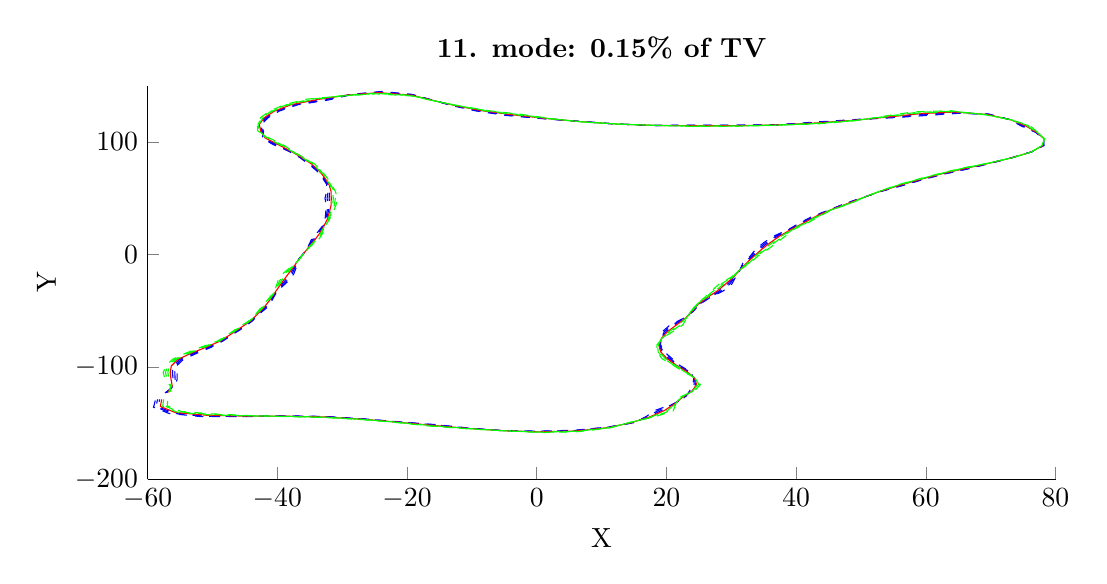
\begin{tikzpicture}

\begin{axis}[%
width=0.95092\figurewidth,
height=\figureheight,
at={(0\figurewidth,0\figureheight)},
scale only axis,
xmin=-60,
xmax=80,
xlabel={X},
ymin=-200,
ymax=150,
ylabel={Y},
title style={font=\bfseries},
title={11. mode: 0.15\% of TV},
axis x line*=bottom,
axis y line*=left
]
\addplot [color=blue,dashed,forget plot]
  table[row sep=crcr]{%
-57.3170072635679	-123.193617991913\\
-55.876739684029	-117.272419186187\\
-55.4495489769981	-111.27245226784\\
-55.4460705138624	-105.368244591195\\
-55.5997940766623	-99.4783657818229\\
-54.4962274803767	-93.5164420613596\\
-52.4408476687975	-88.0491892498165\\
-50.1836912239553	-82.6435323671138\\
-48.3522183144465	-76.9781123157396\\
-46.8539584352749	-71.1382701750411\\
-45.2416964423184	-65.3147202757078\\
-43.8820759073643	-59.4093142363908\\
-42.8717231059305	-53.448907459732\\
-41.6235701793892	-47.5293717607427\\
-40.8801555852936	-41.5264775764333\\
-40.3001599075596	-35.5088387976128\\
-39.3976542769207	-29.5159170732786\\
-38.2563943081755	-23.5005450001296\\
-37.4645952055044	-17.474562386609\\
-37.0611877307175	-11.3873335174931\\
-36.8545202784632	-5.21640787599718\\
-35.9381229072205	0.815433141491916\\
-35.2621960072032	6.86192600592618\\
-34.7525967753931	12.93816371755\\
-33.8667504328636	19.0027331763642\\
-33.024782784982	25.1318120911125\\
-32.6345717762094	31.3065448485007\\
-32.5278549240005	37.4982053111936\\
-32.4552249165765	43.6801957041364\\
-32.6457738972912	49.8669477023173\\
-32.3817001856974	56.0543555244401\\
-32.3975153472445	62.2320802535594\\
-33.0862847502303	68.3247680481629\\
-33.944993194856	74.337922450697\\
-35.1942733280944	80.2667787283373\\
-36.5572429740012	86.1671376712481\\
-38.3430659333282	91.9113552265337\\
-40.5964519900132	97.4343041953283\\
-42.3292002491305	103.076903040343\\
-42.1213218847903	109.190420006325\\
-42.4736143444606	115.302870131089\\
-41.4309509387319	121.429526026018\\
-39.671520301921	127.423346284872\\
-36.8380138944456	132.965478127724\\
-32.1057385791701	137.206940073445\\
-28.2588227217071	142.337100927575\\
-23.8990809003069	144.752812496586\\
-19.2336804511786	142.168439584247\\
-16.25569214765	137.383818467284\\
-13.1404038690126	132.282316970606\\
-9.35037539052481	127.455230894633\\
-4.72717905860936	123.433138146369\\
0.901364441949648	120.621585606669\\
6.64547385341855	118.184094149167\\
12.3169621351817	115.761451646908\\
18.2535493427882	114.526664706929\\
24.6513297898837	114.877293523742\\
30.9275282814353	114.833011332792\\
37.2831802195321	115.219421434316\\
43.3443507274169	117.707943517177\\
49.3620618666342	119.895427611937\\
55.4429423802604	121.577263588504\\
60.3144951116075	123.520565392335\\
64.9001226011367	125.26647146974\\
69.7380613397714	124.660728056744\\
72.9222913411206	119.767135333112\\
74.7366581908871	114.016783261974\\
76.9287773395192	108.44658652086\\
78.1545332917333	102.628615725066\\
78.2272088365078	96.70467637609\\
76.3130877495454	91.0700473650925\\
73.2907818547867	85.9152397480929\\
69.9947697203797	80.9445846889352\\
66.6192929343035	76.0149048493618\\
62.8419602592562	71.358145092457\\
59.5088452823483	66.3341154501739\\
56.4538314254596	61.1377399760759\\
53.1733945893488	56.0374812721656\\
50.4112662356983	50.6600219079611\\
47.6013937846924	45.3081488839617\\
45.2324427780055	39.6924251011184\\
42.6227558519272	34.0401443527713\\
40.6633187189948	28.1821846907523\\
38.8748275027694	22.2600343713121\\
36.6670659230245	16.459613914382\\
35.0548581123722	10.5193633268834\\
33.761967111839	4.46151348039952\\
32.9245437518217	-1.61962494267293\\
31.7996436898177	-7.73269781731519\\
31.316868080537	-14.0259333348193\\
30.6694682415944	-20.288225916419\\
30.0669211529892	-26.5793482657937\\
28.7442627509892	-32.655744696122\\
26.7075162811364	-38.5352013883259\\
25.1163709727697	-44.6066944247331\\
24.1369868570407	-50.7659450944397\\
22.7287348089317	-56.7299103292867\\
20.6493861544337	-62.4191622705269\\
19.4535662437289	-68.393475085782\\
19.1355197827016	-74.4710857233748\\
19.1110674398579	-80.5777619343432\\
19.6661867837289	-86.6815982240964\\
20.8500806896296	-92.6095419607989\\
21.9741885137575	-98.5157625437667\\
23.6893108141479	-104.281269596407\\
24.2163019953628	-109.928171675116\\
24.0931903096397	-115.691198660347\\
23.5660214322451	-121.583289219523\\
22.8543759932033	-127.637843026719\\
20.9993384490845	-133.182023211131\\
18.3187256186831	-138.643613387063\\
16.8700630185974	-144.27148046337\\
15.0625312946003	-149.619499385292\\
10.9070429653573	-153.64864743977\\
5.86937567707214	-156.411575650165\\
0.0689309687431653	-157.223242964954\\
-5.40581829785594	-156.694903187831\\
-10.6420049276822	-154.373316159943\\
-15.6301017714189	-151.381094465785\\
-20.9112015796681	-149.088647035669\\
-26.4739844916421	-146.416353506169\\
-32.5711761007383	-144.163637087517\\
-38.977030356133	-143.596403509744\\
-45.5234777751616	-144.340420684786\\
-51.7043599272184	-144.342727774433\\
-56.7113219569721	-141.451124089849\\
-59.0837182579525	-135.94186567132\\
-58.7742215764944	-128.981345936478\\
};
\addplot [color=blue,dashed,forget plot]
  table[row sep=crcr]{%
-57.1663665279953	-123.037419115377\\
-55.9871697504355	-117.160308069867\\
-55.7636453425755	-111.189816280948\\
-55.8052716796517	-105.28408187532\\
-55.8483907350914	-99.3972429680856\\
-54.7756532564839	-93.4991946680455\\
-52.7181043167204	-88.0211865259542\\
-50.4388330061732	-82.6166841568403\\
-48.4899562380676	-76.9961692898272\\
-46.9689663697731	-71.1535248083793\\
-45.384243158695	-65.3155186875429\\
-43.9759017750407	-59.42427531589\\
-42.9505484892227	-53.4592028226827\\
-41.7786764481828	-47.5184503885676\\
-41.0065162441648	-41.5133669951578\\
-40.3787516935989	-35.4924309192221\\
-39.5357127523454	-29.4859600818463\\
-38.5271095481714	-23.4600269061852\\
-37.7420755727358	-17.4285301121036\\
-37.205837922003	-11.3561862003755\\
-36.8255240293747	-5.2044866298377\\
-35.9303574479358	0.82522120157071\\
-35.2060676831875	6.86968635060722\\
-34.5673393898448	12.9290588431636\\
-33.7189194282561	19.0028082622324\\
-32.9528565120531	25.1405253607207\\
-32.5179300892851	31.3123914625467\\
-32.337455525491	37.4996740183813\\
-32.2064794317762	43.6802698984259\\
-32.3258373234051	49.8655852251812\\
-32.1592843716417	56.048938595796\\
-32.2793846465761	62.2244857141126\\
-32.9634246215641	68.3196756150467\\
-33.823847978685	74.3389672417082\\
-35.0419567148989	80.2914349149899\\
-36.4747432309963	86.1932451025978\\
-38.2419720993713	91.9683491412685\\
-40.3864537369102	97.5543891081532\\
-42.1858782416776	103.217846532278\\
-42.2718875990969	109.295703791652\\
-42.5727612126668	115.373860899974\\
-41.6193763806227	121.463838011951\\
-39.9159581779071	127.424562842782\\
-37.1849093029999	132.963925348263\\
-32.6815930824955	137.313579265156\\
-28.6109142811782	142.040177444788\\
-24.0486171430716	144.401714489795\\
-19.2522586858319	141.938070745781\\
-16.1487930203301	137.167008884254\\
-12.8918188087351	132.179990459477\\
-9.01104715469584	127.482507736024\\
-4.32964914729914	123.587840294136\\
1.10753692792235	120.639548732548\\
6.70317012825516	118.089233666002\\
12.3545148454414	115.761573741981\\
18.2726789465082	114.536796915157\\
24.6000942957106	114.666853998971\\
30.9250703781346	114.669912959421\\
37.2725915339454	115.141115311156\\
43.3408145321858	117.41787411556\\
49.3072028102943	119.693426525052\\
55.1725025399769	121.814921534589\\
59.965221875785	124.044783150612\\
64.7244377768623	125.665495474223\\
69.6514047760632	124.538896567917\\
72.9749617764744	119.722464597191\\
74.9593210396697	114.059874732604\\
76.9846089129625	108.44197875921\\
78.1857627965281	102.618474282554\\
78.1644283594994	96.6932365008895\\
76.3050222942235	91.0420820963991\\
73.2955616650494	85.8927182732241\\
69.9340334919719	80.9656026788888\\
66.4404050695476	76.1121172288505\\
62.7118909241512	71.4166300128099\\
59.3786582633868	66.3967452363487\\
56.303898328643	61.2110784468947\\
53.1275773579231	56.0601068893702\\
50.4256356857431	50.6593774091753\\
47.7242448556304	45.261445242477\\
45.2841807255272	39.6767161596219\\
42.7876814779857	33.9978925463323\\
40.8474409124848	28.1358354623006\\
38.9980039927898	22.2446249649893\\
36.9449083892377	16.409769020917\\
35.3721746989906	10.4568302916528\\
34.0671350373627	4.41227012834675\\
33.114691572986	-1.65154553390957\\
31.9794627845274	-7.76286888580537\\
31.3092142151351	-14.0189595910427\\
30.5670443322578	-20.2568364324792\\
29.7576370152444	-26.4975014014535\\
28.4560044069444	-32.5845891910159\\
26.5727292600416	-38.5007129230278\\
25.0353582621984	-44.5673955728224\\
24.079894943624	-50.7211126148978\\
22.7991845328079	-56.7245920430224\\
20.9586476057053	-62.5038509803826\\
19.7039276979619	-68.4609064121103\\
19.1750849125874	-74.4866300568639\\
19.0139748312373	-80.5777835924476\\
19.4794624928563	-86.6859017123277\\
20.594504966233	-92.636326335508\\
21.8203540179854	-98.5449330988974\\
23.5224894054768	-104.328243604229\\
24.2623527224974	-109.981729216516\\
24.281144083554	-115.731765772983\\
23.6932115032891	-121.561581524127\\
22.7198546391572	-127.525664032264\\
21.0747594556455	-133.163184592333\\
18.7726264899439	-138.731406880031\\
17.0701711880385	-144.343207521757\\
14.9224140942317	-149.616175452825\\
10.962138756443	-153.780347639232\\
5.95476526666652	-156.623294870525\\
0.183849214155636	-157.437688419391\\
-5.35915083362471	-156.7261991624\\
-10.6840848662372	-154.48188423521\\
-15.7750193655351	-151.603345014834\\
-21.035353002386	-149.159642544566\\
-26.5675197180028	-146.493721376927\\
-32.5922555339499	-144.316940803415\\
-38.9162883830287	-143.705785555743\\
-45.3565873301347	-144.17519730339\\
-51.4443120870409	-143.921791152194\\
-56.3951886428177	-141.170253322734\\
-58.7313313885967	-135.734199357459\\
-58.461635602911	-128.969394736228\\
};
\addplot [color=blue,dashed,forget plot]
  table[row sep=crcr]{%
-57.0157257924226	-122.881220238841\\
-56.097599816842	-117.048196953548\\
-56.077741708153	-111.107180294056\\
-56.1644728454411	-105.199919159444\\
-56.0969873935205	-99.3161201543483\\
-55.0550790325912	-93.4819472747315\\
-52.9953609646434	-87.9931838020919\\
-50.6939747883911	-82.5898359465668\\
-48.6276941616887	-77.0142262639147\\
-47.0839743042713	-71.1687794417176\\
-45.5267898750715	-65.316317099378\\
-44.069727642717	-59.4392363953892\\
-43.0293738725149	-53.4694981856333\\
-41.9337827169765	-47.5075290163925\\
-41.1328769030359	-41.5002564138822\\
-40.4573434796381	-35.4760230408314\\
-39.6737712277701	-29.4560030904139\\
-38.7978247881674	-23.4195088122409\\
-38.0195559399672	-17.3824978375983\\
-37.3504881132886	-11.3250388832579\\
-36.7965277802862	-5.19256538367822\\
-35.9225919886512	0.835009261649504\\
-35.1499393591719	6.87744669528827\\
-34.3820820042966	12.9199539687772\\
-33.5710884236487	19.0028833481005\\
-32.8809302391242	25.149238630329\\
-32.4012884023609	31.3182380765929\\
-32.1470561269815	37.501142725569\\
-31.9577339469759	43.6803440927153\\
-32.0059007495191	49.864222748045\\
-31.936868557586	56.043521667152\\
-32.1612539459077	62.2168911746658\\
-32.8405644928979	68.3145831819304\\
-33.7027027625141	74.3400120327193\\
-34.8896401017034	80.3160911016426\\
-36.3922434879913	86.2193525339475\\
-38.1408782654144	92.0253430560032\\
-40.1764554838072	97.6744740209781\\
-42.0425562342247	103.358790024213\\
-42.4224533134034	109.400987576978\\
-42.671908080873	115.444851668859\\
-41.8078018225135	121.498149997884\\
-40.1603960538932	127.425779400691\\
-37.5318047115542	132.962372568802\\
-33.2574475858209	137.420218456867\\
-28.9630058406493	141.743253962001\\
-24.1981533858363	144.050616483005\\
-19.2708369204851	141.707701907314\\
-16.0418938930103	136.950199301223\\
-12.6432337484576	132.077663948349\\
-8.67171891886687	127.509784577415\\
-3.93211923598892	123.742542441903\\
1.31370941389504	120.657511858426\\
6.76086640309177	117.994373182837\\
12.392067555701	115.761695837055\\
18.2918085502281	114.546929123385\\
24.5488588015375	114.456414474199\\
30.9226124748339	114.506814586051\\
37.2620028483587	115.062809187996\\
43.3372783369547	117.127804713943\\
49.2523437539543	119.491425438168\\
54.9020626996934	122.052579480673\\
59.6159486399625	124.56900090889\\
64.5487529525878	126.064519478706\\
69.564748212355	124.41706507909\\
73.0276322118282	119.67779386127\\
75.1819838884523	114.102966203233\\
77.0404404864059	108.43737099756\\
78.2169923013228	102.608332840043\\
78.1016478824911	96.6817966256889\\
76.2969568389017	91.0141168277057\\
73.3003414753121	85.8701967983552\\
69.8732972635641	80.9866206688424\\
66.2615172047916	76.2093296083392\\
62.5818215890462	71.4751149331628\\
59.2484712444253	66.4593750225235\\
56.1539652318264	61.2844169177135\\
53.0817601264975	56.0827325065747\\
50.440005135788	50.6587329103895\\
47.8470959265683	45.2147416009922\\
45.3359186730489	39.6610072181253\\
42.9526071040441	33.9556407398932\\
41.0315631059747	28.0894862338489\\
39.1211804828102	22.2292155586665\\
37.2227508554508	16.359924127452\\
35.6894912856089	10.3942972564221\\
34.3723029628865	4.36302677629398\\
33.3048393941503	-1.68346612514621\\
32.159281879237	-7.79303995429555\\
31.3015603497333	-14.0119858472661\\
30.4646204229212	-20.2254469485394\\
29.4483528774996	-26.4156545371133\\
28.1677460628995	-32.5134336859097\\
26.4379422389468	-38.4662244577297\\
24.9543455516271	-44.5280967209118\\
24.0228030302074	-50.6762801353559\\
22.8696342566841	-56.7192737567582\\
21.2679090569769	-62.5885396902384\\
19.9542891521949	-68.5283377384387\\
19.2146500424732	-74.502174390353\\
18.9168822226168	-80.5778052505521\\
19.2927382019836	-86.6902052005591\\
20.3389292428363	-92.663110710217\\
21.6665195222134	-98.5741036540281\\
23.3556679968058	-104.375217612051\\
24.3084034496319	-110.035286757916\\
24.4690978574683	-115.77233288562\\
23.8204015743331	-121.539873828732\\
22.5853332851112	-127.413485037808\\
21.1501804622065	-133.144345973535\\
19.2265273612047	-138.819200372999\\
17.2702793574797	-144.414934580145\\
14.7822968938631	-149.612851520358\\
11.0172345475286	-153.912047838694\\
6.0401548562609	-156.835014090885\\
0.298767459568107	-157.652133873828\\
-5.31248336939349	-156.757495136969\\
-10.7261648047922	-154.590452310476\\
-15.9199369596514	-151.825595563883\\
-21.159504425104	-149.230638053463\\
-26.6610549443634	-146.571089247685\\
-32.6133349671615	-144.470244519314\\
-38.8555464099243	-143.815167601741\\
-45.1896968851078	-144.009973921993\\
-51.1842642468634	-143.500854529954\\
-56.0790553286633	-140.889382555619\\
-58.3789445192408	-135.526533043598\\
-58.1490496293277	-128.957443535978\\
};
\addplot [color=red,solid,forget plot]
  table[row sep=crcr]{%
-56.8650850568499	-122.725021362305\\
-56.2080298832485	-116.936085837228\\
-56.3918380737305	-111.024544307164\\
-56.5236740112305	-105.115756443569\\
-56.3455840519496	-99.234997340611\\
-55.3345048086984	-93.4646998814174\\
-53.2726176125663	-87.9651810782296\\
-50.949116570609	-82.5629877362933\\
-48.7654320853097	-77.0322832380022\\
-47.1989822387695	-71.1840340750558\\
-45.6693365914481	-65.317115511213\\
-44.1635535103934	-59.4541974748884\\
-43.1081992558071	-53.479793548584\\
-42.0888889857701	-47.4966076442174\\
-41.2592375619071	-41.4871458326067\\
-40.5359352656773	-35.4596151624407\\
-39.8118297031948	-29.4260460989816\\
-39.0685400281634	-23.3789907182966\\
-38.2970363071987	-17.3364655630929\\
-37.4951383045741	-11.2938915661403\\
-36.7675315311977	-5.18064413751875\\
-35.9148265293666	0.844797321728298\\
-35.0938110351563	6.88520703996931\\
-34.1968246187483	12.9108490943909\\
-33.4232574190412	19.0029584339687\\
-32.8090039661952	25.1579518999372\\
-32.2846467154367	31.324084690639\\
-31.956656728472	37.5026114327567\\
-31.7089884621756	43.6804182870047\\
-31.685964175633	49.8628602709089\\
-31.7144527435303	56.038104738508\\
-32.0431232452393	62.209296635219\\
-32.7177043642317	68.3094907488142\\
-33.5815575463431	74.3410568237305\\
-34.737323488508	80.3407472882952\\
-36.3097437449864	86.2454599652972\\
-38.0397844314575	92.082336970738\\
-39.9664572307042	97.794558933803\\
-41.8992342267718	103.499733516148\\
-42.57301902771	109.506271362305\\
-42.7710549490792	115.515842437744\\
-41.9962272644043	121.532461983817\\
-40.4048339298793	127.426995958601\\
-37.8787001201085	132.960819789342\\
-33.8333020891462	137.526857648577\\
-29.3150974001203	141.446330479213\\
-24.3476896286011	143.699518476214\\
-19.2894151551383	141.477333068848\\
-15.9349947656904	136.733389718192\\
-12.3946486881801	131.975337437221\\
-8.33239068303789	127.537061418806\\
-3.53458932467869	123.897244589669\\
1.51988189986774	120.675474984305\\
6.81856267792838	117.899512699672\\
12.4296202659607	115.761817932129\\
18.3109381539481	114.557061331613\\
24.4976233073643	114.245974949428\\
30.9201545715332	114.343716212681\\
37.251414162772	114.984503064837\\
43.3337421417236	116.837735312326\\
49.1974846976144	119.289424351283\\
54.6316228594099	122.290237426758\\
59.2666754041399	125.093218667167\\
64.3730681283133	126.463543483189\\
69.4780916486468	124.295233590262\\
73.0803026471819	119.633123125349\\
75.4046467372349	114.146057673863\\
77.0962720598493	108.43276323591\\
78.2482218061175	102.598191397531\\
78.0388674054827	96.6703567504883\\
76.2888913835798	90.9861515590123\\
73.3051212855748	85.8476753234863\\
69.8125610351563	81.007638658796\\
66.0826293400356	76.3065419878278\\
62.4517522539411	71.5335998535156\\
59.1182842254639	66.5220048086984\\
56.0040321350098	61.3577553885324\\
53.0359428950718	56.1053581237793\\
50.4543745858329	50.6580884116037\\
47.9699469975063	45.1680379595075\\
45.3876566205706	39.6452982766288\\
43.1175327301025	33.9133889334542\\
41.2156852994646	28.0431370053973\\
39.2443569728306	22.2138061523438\\
37.500593321664	16.310079233987\\
36.0068078722273	10.3317642211914\\
34.6774708884103	4.3137834242412\\
33.4949872153146	-1.71538671638284\\
32.3391009739467	-7.82321102278573\\
31.2939064843314	-14.0050121034895\\
30.3621965135847	-20.1940574645996\\
29.1390687397548	-26.3338076727731\\
27.8794877188546	-32.4422781808036\\
26.3031552178519	-38.4317359924316\\
24.8733328410557	-44.4887978690011\\
23.9657111167908	-50.631447655814\\
22.9400839805603	-56.7139554704939\\
21.5771705082485	-62.6732284000942\\
20.2046506064279	-68.595769064767\\
19.2542151723589	-74.5177187238421\\
18.8197896139962	-80.5778269086565\\
19.106013911111	-86.6945086887905\\
20.0833535194397	-92.6898950849261\\
21.5126850264413	-98.6032742091588\\
23.1888465881348	-104.422191619873\\
24.3544541767665	-110.088844299316\\
24.6570516313825	-115.812899998256\\
23.947591645377	-121.518166133336\\
22.4508119310652	-127.301306043352\\
21.2256014687674	-133.125507354736\\
19.6804282324655	-138.906993865967\\
17.4703875269209	-144.486661638532\\
14.6421796934945	-149.609527587891\\
11.0723303386143	-154.043748038156\\
6.12554444585528	-157.046733311244\\
0.413685704980578	-157.866579328265\\
-5.26581590516227	-156.788791111537\\
-10.7682447433472	-154.699020385742\\
-16.0648545537676	-152.047846112932\\
-21.2836558478219	-149.30163356236\\
-26.7545901707241	-146.648457118443\\
-32.6344144003732	-144.623548235212\\
-38.7948044368199	-143.92454964774\\
-45.0228064400809	-143.844750540597\\
-50.924216406686	-143.079917907715\\
-55.7629220145089	-140.608511788504\\
-58.0265576498849	-135.318866729736\\
-57.8364636557443	-128.945492335728\\
};
\addplot [color=green,dashed,forget plot]
  table[row sep=crcr]{%
-56.7144443212772	-122.568822485769\\
-56.3184599496549	-116.823974720908\\
-56.7059344393079	-110.941908320272\\
-56.8828751770198	-105.031593727693\\
-56.5941807103787	-99.1538745268738\\
-55.6139305848056	-93.4474524881034\\
-53.5498742604892	-87.9371783543673\\
-51.2042583528269	-82.5361395260197\\
-48.9031700089308	-77.0503402120898\\
-47.3139901732677	-71.1992887083941\\
-45.8118833078247	-65.3179139230481\\
-44.2573793780698	-59.4691585543876\\
-43.1870246390992	-53.4900889115346\\
-42.2439952545637	-47.4856862720422\\
-41.3855982207782	-41.4740352513312\\
-40.6145270517166	-35.44320728405\\
-39.9498881786194	-29.3960891075492\\
-39.3392552681593	-23.3384726243523\\
-38.5745166744301	-17.2904332885876\\
-37.6397884958597	-11.2627442490227\\
-36.7385352821092	-5.16872289135927\\
-35.907061070082	0.854585381807092\\
-35.0376827111406	6.89296738465035\\
-34.0115672332	12.9017442200045\\
-33.2754264144338	19.0030335198368\\
-32.7370776932663	25.1666651695455\\
-32.1680050285124	31.3299313046851\\
-31.7662573299625	37.5040801399444\\
-31.4602429773753	43.6804924812942\\
-31.366027601747	49.8614977937728\\
-31.4920369294746	56.0326878098639\\
-31.9249925445708	62.2017020957722\\
-32.5948442355654	68.3043983156979\\
-33.4604123301722	74.3421016147416\\
-34.5850068753125	80.3654034749478\\
-36.2272440019815	86.2715673966469\\
-37.9386905975006	92.1393308854728\\
-39.7564589776012	97.9146438466279\\
-41.7559122193189	103.640677008083\\
-42.7235847420165	109.611555147631\\
-42.8702018172854	115.586833206629\\
-42.1846527062951	121.56677396975\\
-40.6492718058654	127.42821251651\\
-38.2255955286628	132.959267009881\\
-34.4091565924716	137.633496840288\\
-29.6671889595914	141.149406996426\\
-24.4972258713658	143.348420469423\\
-19.3079933897915	141.246964230381\\
-15.8280956383705	136.516580135161\\
-12.1460636279026	131.873010926093\\
-7.99306244720892	127.564338260197\\
-3.13705941336847	124.051946737436\\
1.72605438584044	120.693438110184\\
6.87625895276499	117.804652216507\\
12.4671729762203	115.761940027203\\
18.3300677576681	114.567193539841\\
24.4463878131912	114.035535424657\\
30.9176966682325	114.180617839311\\
37.2408254771854	114.906196941677\\
43.3302059464925	116.547665910708\\
49.1426256412745	119.087423264399\\
54.3611830191264	122.527895372842\\
58.9174021683174	125.617436425444\\
64.1973833040389	126.862567487672\\
69.3914350849386	124.173402101435\\
73.1329730825357	119.588452389428\\
75.6273095860175	114.189149144493\\
77.1521036332927	108.42815547426\\
78.2794513109122	102.588049955019\\
77.9760869284743	96.6589168752877\\
76.2808259282579	90.9581862903189\\
73.3099010958374	85.8251538486175\\
69.7518248067484	81.0286566487496\\
65.9037414752796	76.4037543673165\\
62.3216829188361	71.5920847738685\\
58.9880972065024	66.5846345948732\\
55.8540990381931	61.4310938593512\\
52.9901256636462	56.1279837409839\\
50.4687440358777	50.6574439128178\\
48.0927980684442	45.1213343180228\\
45.4393945680923	39.6295893351322\\
43.282458356161	33.8711371270152\\
41.3998074929546	27.9967877769456\\
39.367533462851	22.198396746021\\
37.7784357878771	16.260234340522\\
36.3241244588456	10.2692311859607\\
34.9826388139341	4.26454007218843\\
33.6851350364789	-1.74730730761948\\
32.5189200686564	-7.85338209127591\\
31.2862526189295	-13.9980383597129\\
30.2597726042481	-20.1626679806598\\
28.82978460201	-26.2519608084329\\
27.5912293748098	-32.3711226756974\\
26.1683681967571	-38.3972475271336\\
24.7923201304844	-44.4494990170905\\
23.9086192033741	-50.5866151762721\\
23.0105337044365	-56.7086371842296\\
21.8864319595201	-62.7579171099499\\
20.4550120606609	-68.6632003910954\\
19.2937803022447	-74.5332630573312\\
18.7226970053757	-80.577848566761\\
18.9192896202384	-86.6988121770218\\
19.827777796043	-92.7166794596351\\
21.3588505306692	-98.6324447642894\\
23.0220251794637	-104.469165627695\\
24.4005049039011	-110.142401840717\\
24.8450054052968	-115.853467110893\\
24.074781716421	-121.49645843794\\
22.3162905770191	-127.189127048897\\
21.3010224753284	-133.106668735938\\
20.1343291037263	-138.994787358935\\
17.670495696362	-144.55838869692\\
14.5020624931259	-149.606203655423\\
11.1274261297	-154.175448237617\\
6.21093403544966	-157.258452531604\\
0.528603950393049	-158.081024782701\\
-5.21914844093104	-156.820087086106\\
-10.8103246819022	-154.807588461008\\
-16.2097721478839	-152.270096661982\\
-21.4078072705398	-149.372629071258\\
-26.8481253970847	-146.725824989201\\
-32.6554938335848	-144.77685195111\\
-38.7340624637155	-144.033931693739\\
-44.855915995054	-143.679527159201\\
-50.6641685665085	-142.658981285475\\
-55.4467887003546	-140.327641021389\\
-57.674170780529	-135.111200415875\\
-57.5238776821609	-128.933541135478\\
};
\addplot [color=green,dashed,forget plot]
  table[row sep=crcr]{%
-56.5638035857045	-122.412623609233\\
-56.4288900160614	-116.711863604588\\
-57.0200308048854	-110.85927233338\\
-57.2420763428092	-104.947431011818\\
-56.8427773688079	-99.0727517131365\\
-55.8933563609128	-93.4302050947893\\
-53.8271309084121	-87.9091756305051\\
-51.4594001350447	-82.5092913157462\\
-49.0409079325518	-77.0683971861773\\
-47.4289981077659	-71.2145433417323\\
-45.9544300242012	-65.3187123348832\\
-44.3512052457461	-59.4841196338868\\
-43.2658500223914	-53.5003842744853\\
-42.3991015233574	-47.4747648998671\\
-41.5119588796494	-41.4609246700557\\
-40.6931188377558	-35.4267994056593\\
-40.0879466540441	-29.3661321161169\\
-39.6099705081553	-23.2979545304079\\
-38.8519970416615	-17.2444010140822\\
-37.7844386871453	-11.2315969319051\\
-36.7095390330207	-5.15680164519979\\
-35.8992956107974	0.864373441885886\\
-34.981554387125	6.90072772933139\\
-33.8263098476517	12.8926393456181\\
-33.1275954098263	19.003108605705\\
-32.6651514203374	25.1753784391537\\
-32.0513633415882	31.3357779187312\\
-31.5758579314531	37.5055488471321\\
-31.211497492575	43.6805666755836\\
-31.0460910278609	49.8601353166366\\
-31.2696211154189	56.0272708812199\\
-31.8068618439024	62.1941075563254\\
-32.4719841068992	68.2993058825817\\
-33.3392671140012	74.3431464057528\\
-34.432690262117	80.3900596616005\\
-36.1447442589765	86.2976748279966\\
-37.8375967635437	92.1963248002075\\
-39.5464607244982	98.0347287594528\\
-41.612590211866	103.781620500018\\
-42.8741504563231	109.716838932958\\
-42.9693486854916	115.657823975514\\
-42.3730781481859	121.601085955683\\
-40.8937096818516	127.42942907442\\
-38.572490937217	132.95771423042\\
-34.9850110957969	137.740136031998\\
-30.0192805190625	140.852483513638\\
-24.6467621141305	142.997322462632\\
-19.3265716244447	141.016595391915\\
-15.7211965110507	136.29977055213\\
-11.8974785676251	131.770684414965\\
-7.65373421137995	127.591615101588\\
-2.73952950205825	124.206648885203\\
1.93222687181313	120.711401236063\\
6.9339552276016	117.709791733342\\
12.50472568648	115.762062122276\\
18.3491973613881	114.577325748069\\
24.3951523190181	113.825095899885\\
30.9152387649318	114.017519465941\\
37.2302367915987	114.827890818518\\
43.3266697512615	116.257596509091\\
49.0877665849345	118.885422177515\\
54.0907431788429	122.765553318927\\
58.5681289324949	126.141654183721\\
64.0216984797644	127.261591492155\\
69.3047785212303	124.051570612608\\
73.1856435178894	119.543781653507\\
75.8499724348002	114.232240615122\\
77.2079352067361	108.42354771261\\
78.3106808157069	102.577908512507\\
77.913306451466	96.6474770000871\\
76.2727604729361	90.9302210216255\\
73.3146809061001	85.8026323737486\\
69.6910885783406	81.0496746387033\\
65.7248536105236	76.5009667468052\\
62.1916135837311	71.6505696942214\\
58.8579101875409	66.647264381048\\
55.7041659413765	61.50443233017\\
52.9443084322206	56.1506093581884\\
50.4831134859226	50.656799414032\\
48.2156491393822	45.0746306765381\\
45.4911325156139	39.6138803936356\\
43.4473839822194	33.8288853205762\\
41.5839296864445	27.9504385484939\\
39.4907099528714	22.1829873396982\\
38.0562782540903	16.210389447057\\
36.6414410454639	10.2066981507301\\
35.2878067394578	4.21529672013565\\
33.8752828576432	-1.77922789885612\\
32.698739163366	-7.88355315976609\\
31.2785987535277	-13.9910646159363\\
30.1573486949116	-20.13127849672\\
28.5205004642652	-26.1701139440927\\
27.3029710307649	-32.2999671705913\\
26.0335811756622	-38.3627590618355\\
24.7113074199131	-44.4102001651798\\
23.8515272899575	-50.5417826967302\\
23.0809834283127	-56.7033188979653\\
22.1956934107917	-62.8426058198057\\
20.7053735148939	-68.7306317174237\\
19.3333454321304	-74.5488073908203\\
18.6256043967551	-80.5778702248654\\
18.7325653293658	-86.7031156652532\\
19.5722020726464	-92.7434638343442\\
21.2050160348972	-98.6616153194202\\
22.8552037707927	-104.516139635517\\
24.4465556310357	-110.195959382117\\
25.0329591792111	-115.894034223529\\
24.2019717874649	-121.474750742544\\
22.1817692229731	-127.076948054441\\
21.3764434818894	-133.08783011714\\
20.5882299749871	-139.082580851902\\
17.8706038658032	-144.630115755307\\
14.3619452927573	-149.602879722956\\
11.1825219207857	-154.307148437079\\
6.29632362504403	-157.470171751964\\
0.643522195805519	-158.295470237138\\
-5.17248097669982	-156.851383060675\\
-10.8524046204572	-154.916156536275\\
-16.3546897420001	-152.492347211031\\
-21.5319586932578	-149.443624580155\\
-26.9416606234453	-146.803192859959\\
-32.6765732667965	-144.930155667009\\
-38.6733204906111	-144.143313739737\\
-44.6890255500271	-143.514303777805\\
-50.404120726331	-142.238044663236\\
-55.1306553862002	-140.046770254274\\
-57.3217839111732	-134.903534102014\\
-57.2112917085775	-128.921589935229\\
};
\addplot [color=green,dashed,forget plot]
  table[row sep=crcr]{%
-56.4131628501318	-122.256424732697\\
-56.5393200824679	-116.599752488269\\
-57.3341271704629	-110.776636346488\\
-57.6012775085986	-104.863268295942\\
-57.091374027237	-98.9916288993992\\
-56.1727821370201	-93.4129577014752\\
-54.104387556335	-87.8811729066428\\
-51.7145419172626	-82.4824431054727\\
-49.1786458561729	-77.0864541602649\\
-47.5440060422642	-71.2297979750705\\
-46.0969767405778	-65.3195107467183\\
-44.4450311134225	-59.499080713386\\
-43.3446754056836	-53.510679637436\\
-42.554207792151	-47.463843527692\\
-41.6383195385206	-41.4478140887802\\
-40.771710623795	-35.4103915272686\\
-40.2260051294688	-29.3361751246845\\
-39.8806857481513	-23.2574364364636\\
-39.129477408893	-17.1983687395769\\
-37.9290888784308	-11.2004496147876\\
-36.6805427839322	-5.14488039904032\\
-35.8915301515128	0.874161501964679\\
-34.9254260631093	6.90848807401243\\
-33.6410524621034	12.8835344712318\\
-32.9797644052189	19.0031836915732\\
-32.5932251474085	25.184091708762\\
-31.934721654664	31.3416245327773\\
-31.3854585329436	37.5070175543198\\
-30.9627520077747	43.680640869873\\
-30.7261544539749	49.8587728395005\\
-31.0472053013632	56.0218539525758\\
-31.688731143234	62.1865130168786\\
-32.349123978233	68.2942134494654\\
-33.2181218978302	74.3441911967639\\
-34.2803736489215	80.4147158482531\\
-36.0622445159716	86.3237822593463\\
-37.7365029295868	92.2533187149423\\
-39.3364624713952	98.1548136722777\\
-41.4692682044131	103.922563991954\\
-43.0247161706296	109.822122718284\\
-43.0684955536978	115.728814744399\\
-42.5615035900766	121.635397941615\\
-41.1381475578377	127.430645632329\\
-38.9193863457713	132.956161450959\\
-35.5608655991223	137.846775223709\\
-30.3713720785335	140.555560030851\\
-24.7962983568953	142.646224455841\\
-19.3451498590979	140.786226553448\\
-15.6142973837308	136.0829609691\\
-11.6488935073476	131.668357903836\\
-7.31440597555098	127.618891942979\\
-2.34199959074802	124.36135103297\\
2.13839935778583	120.729364361942\\
6.9916515024382	117.614931250177\\
12.5422783967396	115.76218421735\\
18.368326965108	114.587457956297\\
24.3439168248449	113.614656375114\\
30.9127808616312	113.854421092571\\
37.219648106012	114.749584695358\\
43.3231335560304	115.967527107474\\
49.0329075285946	118.68342109063\\
53.8203033385593	123.003211265012\\
58.2188556966723	126.665871941998\\
63.8460136554899	127.660615496639\\
69.2181219575221	123.92973912378\\
73.2383139532432	119.499110917586\\
76.0726352835828	114.275332085752\\
77.2637667801795	108.41893995096\\
78.3419103205016	102.567767069995\\
77.8505259744576	96.6360371248865\\
76.2646950176142	90.9022557529321\\
73.3194607163628	85.7801108988797\\
69.6303523499328	81.0706926286569\\
65.5459657457676	76.5981791262939\\
62.0615442486261	71.7090546145742\\
58.7277231685794	66.7098941672229\\
55.5542328445599	61.5777708009889\\
52.8984912007949	56.173234975393\\
50.4974829359675	50.6561549152462\\
48.3385002103202	45.0279270350534\\
45.5428704631356	39.5981714521391\\
43.6123096082779	33.7866335141372\\
41.7680518799345	27.9040893200422\\
39.6138864428919	22.1675779333754\\
38.3341207203034	16.160544553592\\
36.9587576320823	10.1441651154994\\
35.5929746649816	4.16605336808288\\
34.0654306788075	-1.81114849009276\\
32.8785582580757	-7.91372422825627\\
31.2709448881258	-13.9840908721597\\
30.054924785575	-20.0998890127802\\
28.2112163265204	-26.0882670797524\\
27.01471268672	-32.2288116654851\\
25.8987941545674	-38.3282705965374\\
24.6302947093418	-44.3709013132692\\
23.7944353765409	-50.4969502171883\\
23.1514331521889	-56.698000611701\\
22.5049548620633	-62.9272945296615\\
20.9557349691269	-68.7980630437521\\
19.3729105620162	-74.5643517243093\\
18.5285117881346	-80.5778918829699\\
18.5458410384932	-86.7074191534846\\
19.3166263492498	-92.7702482090532\\
21.0511815391251	-98.6907858745508\\
22.6883823621216	-104.563113643339\\
24.4926063581703	-110.249516923517\\
25.2209129531254	-115.934601336166\\
24.3291618585089	-121.453043047148\\
22.047247868927	-126.964769059986\\
21.4518644884504	-133.068991498342\\
21.0421308462479	-139.17037434487\\
18.0707120352443	-144.701842813695\\
14.2218280923887	-149.599555790489\\
11.2376177118714	-154.438848636541\\
6.38171321463841	-157.681890972324\\
0.75844044121799	-158.509915691575\\
-5.12581351246859	-156.882679035244\\
-10.8944845590122	-155.024724611541\\
-16.4996073361164	-152.71459776008\\
-21.6561101159757	-149.514620089052\\
-27.035195849806	-146.880560730717\\
-32.6976527000081	-145.083459382907\\
-38.6125785175067	-144.252695785736\\
-44.5221351050002	-143.349080396408\\
-50.1440728861535	-141.817108040997\\
-54.8145220720458	-139.765899487159\\
-56.9693970418173	-134.695867788152\\
-56.8987057349942	-128.909638734979\\
};
\end{axis}
\end{tikzpicture}%
					\caption{Modus 11}
					\label{fig:mode11}
				\end{subfigure}	
				\quad
				\begin{subfigure}{0.3\textwidth}
					\centering
					% This file was created by matlab2tikz.
% Minimal pgfplots version: 1.3
%
%The latest updates can be retrieved from
%  http://www.mathworks.com/matlabcentral/fileexchange/22022-matlab2tikz
%where you can also make suggestions and rate matlab2tikz.
%
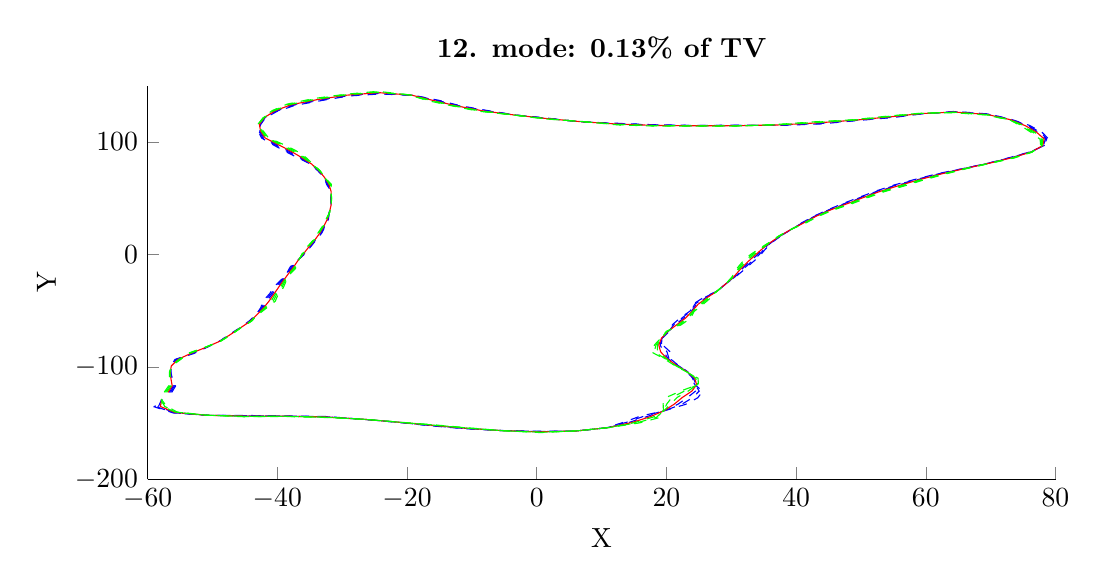
\begin{tikzpicture}

\begin{axis}[%
width=0.95092\figurewidth,
height=\figureheight,
at={(0\figurewidth,0\figureheight)},
scale only axis,
xmin=-60,
xmax=80,
xlabel={X},
ymin=-200,
ymax=150,
ylabel={Y},
title style={font=\bfseries},
title={12. mode: 0.13\% of TV},
axis x line*=bottom,
axis y line*=left
]
\addplot [color=blue,dashed,forget plot]
  table[row sep=crcr]{%
-56.2877683221313	-122.819005577942\\
-55.6926489656939	-117.17225078183\\
-56.153245567768	-111.305006512111\\
-56.396064059229	-105.436483233664\\
-56.4369445103214	-99.4522113529489\\
-55.7744118894845	-93.4556611674677\\
-52.8890658360947	-88.2141827477903\\
-50.8335023155775	-82.628264987306\\
-48.832504530046	-76.9642565645718\\
-47.3467380802382	-71.0861791249472\\
-45.7102023727465	-65.2334903912742\\
-44.3327368701808	-59.319513418999\\
-43.2445584642436	-53.3436309212654\\
-42.5403471159094	-47.3108324636748\\
-42.1994557804552	-41.2341841241802\\
-41.2001423151719	-35.2354820594682\\
-40.5532611890399	-29.2252624778871\\
-39.5103938689984	-23.2520225605544\\
-38.5823037529719	-17.272293786451\\
-38.0127507214347	-11.226935055381\\
-36.8465221745726	-5.16794082635126\\
-35.6758467872638	0.802995652191127\\
-34.850254928129	6.80829316218536\\
-33.9846182801043	12.8225060162064\\
-33.1400138642335	18.8930187503565\\
-32.6155023427325	25.0692347245313\\
-32.1040410434807	31.2373518308977\\
-32.0094490581211	37.4351674473716\\
-31.7190842905532	43.6267910477416\\
-31.7506841480633	49.8206744999887\\
-31.695295747217	56.0168652987284\\
-32.4098638920163	62.1849204846795\\
-32.7697094789966	68.3318541258907\\
-33.7765729051546	74.4006579983794\\
-34.9244219584225	80.3816711117229\\
-36.9863686232636	86.1711934980397\\
-38.9224521247355	91.9033413470044\\
-40.7143596450049	97.5666381945195\\
-42.4178744042874	103.340456272198\\
-42.980717222167	109.387125850651\\
-42.5534737912173	115.446605960614\\
-41.8435152584673	121.320726203094\\
-40.0346127593084	127.064025356908\\
-37.3220324714776	132.348584475124\\
-33.1571558162822	136.707362986205\\
-28.9435184744572	140.740224066514\\
-24.169066024896	142.536927514041\\
-18.8515271283847	141.169095729799\\
-15.0085450020954	136.776559548161\\
-11.7201189568958	131.972805076988\\
-7.58793500757294	127.794873976539\\
-3.29012755654847	123.819269244727\\
1.73228103624423	121.006624815619\\
6.55441803891576	117.778702022699\\
12.3125599744128	116.504168692378\\
18.0170300697618	115.171808526552\\
24.1864379497614	114.551528506375\\
30.8121788512349	114.751201718056\\
37.3877627062867	114.504469973521\\
43.8110996151907	115.890383933345\\
49.5381322634282	118.977429941106\\
54.9877664677253	121.61480823042\\
59.0590495783019	124.606497693744\\
64.4498714001972	127.027877002144\\
69.7230431792161	124.71181266531\\
73.1885968677708	119.932031488164\\
75.9986644076634	114.561508524477\\
77.8602375272781	108.837280857152\\
78.8669991556238	102.945714982662\\
78.362625377343	96.9579842756804\\
76.2266664235181	91.2978719801121\\
73.0301199599067	86.1436217035892\\
69.6973038369802	81.1158266830922\\
65.9013594137377	76.4453286886116\\
61.9877522349208	71.8774820811167\\
58.5372603655729	66.9024017062852\\
55.2321525328036	61.802540803615\\
52.4029755848101	56.4396228751584\\
49.8544801327563	50.9490247642649\\
47.359061193569	45.4369268426043\\
44.9773039981651	39.7898722887824\\
42.7974335395496	34.0321989936464\\
40.9208114278955	28.1643251019756\\
39.2606324376558	22.2178188818521\\
37.6619868897446	16.2491252543303\\
36.1926045145137	10.2378432343966\\
35.1861425105494	4.12956588593852\\
34.3276313865143	-1.96373708818485\\
33.0923120325478	-8.01794412722133\\
31.8998088127962	-14.1548550141212\\
30.6100466091998	-20.2548130540926\\
29.1534480373369	-26.2867292824154\\
27.9169220293044	-32.4060791989251\\
25.754738643666	-38.2752108178591\\
24.1467788189877	-44.2274008137419\\
23.6682937187684	-50.4063870870526\\
22.1583780006454	-56.4264322840455\\
20.9471700545385	-62.4436760880769\\
20.4119872986587	-68.7364196048841\\
19.3247696439102	-74.7603768009715\\
19.4511006071931	-80.7793610559894\\
20.5805719852074	-86.7292165897387\\
20.5399154890023	-92.5790506101127\\
21.795174686236	-98.5224563087887\\
23.2894663320249	-104.355139708429\\
23.8261446150399	-109.970260525096\\
24.3817584950031	-115.882802330943\\
25.5916623125725	-121.726202490316\\
24.8346651961431	-127.580215191853\\
22.9552149616934	-133.401747490012\\
19.8238703367094	-138.895807443873\\
15.9341960331034	-143.962189495539\\
13.3859495361422	-149.379048465212\\
10.6717764981698	-154.287517789476\\
5.86112009218754	-157.226464683234\\
0.153214505527343	-157.221786899334\\
-5.49607654937251	-156.657330744021\\
-11.124805011295	-155.037673805754\\
-16.3946890228821	-152.438658765553\\
-21.4277968278854	-149.373110401189\\
-26.8261467385128	-146.664683424106\\
-32.5740836453176	-144.180418986893\\
-38.7367548090719	-143.678808773719\\
-44.9732769346226	-143.279653210967\\
-50.9055496841011	-143.131715651803\\
-56.0623968210765	-141.013904148167\\
-58.9839286505891	-135.574715124404\\
-57.7534228450591	-129.205844850324\\
};
\addplot [color=blue,dashed,forget plot]
  table[row sep=crcr]{%
-56.4802072337041	-122.787677506063\\
-55.8644426048788	-117.093529133629\\
-56.2327764030888	-111.211519110462\\
-56.4386007098962	-105.329574303632\\
-56.4064910241975	-99.3798066821696\\
-55.6277761958891	-93.4586740721176\\
-53.0169164282519	-88.1311821912701\\
-50.872040400588	-82.6065059036351\\
-48.8101470484672	-76.9869321223819\\
-47.297486133082	-71.11879744165\\
-45.696580445647	-65.2613654312538\\
-44.2763424169184	-59.3644081042954\\
-43.1991053947648	-53.3890184637049\\
-42.3898610725296	-47.3727575238556\\
-41.8860497076059	-41.3185046936557\\
-40.9787399653403	-35.3101930937924\\
-40.3061173604248	-29.2921903515853\\
-39.3631092553867	-23.2943452798018\\
-38.4872146043808	-17.2936843786649\\
-37.8402132491478	-11.2492538923008\\
-36.8201919601143	-5.17217526340709\\
-35.7555067012981	0.81692954203685\\
-34.9314402971381	6.83393112144668\\
-34.055353726319	12.8519537089346\\
-33.2344283825027	18.9296653115606\\
-32.6800028838867	25.0988071163333\\
-32.1642429341327	31.2662627841448\\
-31.9918516149048	37.4576487758333\\
-31.7157190144273	43.6446667941626\\
-31.7291108239198	49.8347364236288\\
-31.7016814126547	56.0239451119883\\
-32.2876170097573	62.1930458681926\\
-32.7523744407416	68.3243996668652\\
-33.7115677855508	74.3807909401631\\
-34.8620558017843	80.368029837247\\
-36.7608269971712	86.1959489871255\\
-38.6282295603095	91.9630065549156\\
-40.465058840238	97.6426117742806\\
-42.2449943451156	103.393548686848\\
-42.8448178240147	109.426841021202\\
-42.6260008438379	115.469684786324\\
-41.8944192604463	121.391304796668\\
-40.1580198161654	127.185015557472\\
-37.5075883543546	132.552662913196\\
-33.3825379072369	136.980527873662\\
-29.0673781163449	140.975592870747\\
-24.228607226131	142.924457834765\\
-18.9974898039692	141.271841509482\\
-15.3173615899604	136.762169604838\\
-11.9449622006572	131.973649197065\\
-7.83608689939459	127.708936457295\\
-3.37161481259188	123.845261026374\\
1.66148132411873	120.896241538514\\
6.64246625191996	117.818972248357\\
12.3515800715954	116.256718438962\\
18.1149994311572	114.966892794906\\
24.2901664022957	114.449677320726\\
30.848170758001	114.615373216264\\
37.3423131917818	114.664481003959\\
43.6519804573683	116.206167726338\\
49.4245830748236	119.081428077832\\
54.8690519316201	121.839951295866\\
59.1282581869146	124.768738018218\\
64.4242703095693	126.839765829159\\
69.6413926690263	124.572952973628\\
73.1524987942412	119.832395367226\\
75.8006585175206	114.423024907605\\
77.6055823714685	108.702441650071\\
78.6607400391217	102.829873787618\\
78.2547060533896	96.8621084339497\\
76.247408076872	91.1939651730788\\
73.1217870684628	86.0449729102216\\
69.7357229030389	81.0797640083268\\
65.9617827225036	76.399066455017\\
62.1424189079276	71.7628546719164\\
58.7309349855366	66.775602740423\\
55.489445733539	61.6542789985874\\
52.6139646882307	56.3282012913654\\
50.0544449504485	50.8520459800445\\
47.5626897948814	45.3472972149054\\
45.1140882056336	39.7416809513979\\
42.9041332697339	33.992595640249\\
41.0191027184185	28.1239290697829\\
39.2552072827141	22.2164813053493\\
37.6081890337178	16.2694432475492\\
36.1306723004182	10.2691502299949\\
35.0165853031697	4.19097173203941\\
34.0500833294477	-1.88095363091751\\
32.8412416796808	-7.95303309240946\\
31.6978413699746	-14.1049073772439\\
30.5274299106614	-20.2345611909283\\
29.1486549381428	-26.3024220792013\\
27.9044439258212	-32.4181455262179\\
25.9375441683946	-38.3273858760499\\
24.3889634930104	-44.314533165495\\
23.7674328514425	-50.4814072766397\\
22.418946660617	-56.522273346195\\
21.1571702057751	-62.520193525416\\
20.3428750679151	-68.6895360915118\\
19.3012514867265	-74.6794907752617\\
19.2406636094608	-80.7121830068785\\
20.0890526271753	-86.7176472894226\\
20.3877281658148	-92.6159987683838\\
21.7010114663045	-98.5493956089121\\
23.2559264173949	-104.377490345577\\
24.0022478022821	-110.009788449836\\
24.4735228737962	-115.85950155338\\
25.0436387568407	-121.656857037989\\
24.0400474411171	-127.487245475686\\
22.3786771307181	-133.30966744492\\
19.7760563019614	-138.899536251237\\
16.4462598643759	-144.137013543203\\
13.8046929219263	-149.455874839438\\
10.8052944449846	-154.206261205702\\
5.94926154341012	-157.166554225904\\
0.240038238678421	-157.436717708977\\
-5.41932300130243	-156.701150866527\\
-11.0059515886457	-154.924789332417\\
-16.2847441998439	-152.308387881346\\
-21.3797498345309	-149.349284788246\\
-26.8022945492499	-146.659274655552\\
-32.5941938970028	-144.328128736333\\
-38.7561046849879	-143.760722398392\\
-44.9897867697754	-143.46801898751\\
-50.9117719249627	-143.114449737107\\
-55.962571885554	-140.878773361613\\
-58.6648049836877	-135.489432326181\\
-57.7811031152875	-129.119060678792\\
};
\addplot [color=blue,dashed,forget plot]
  table[row sep=crcr]{%
-56.672646145277	-122.756349434184\\
-56.0362362440636	-117.014807485429\\
-56.3123072384096	-111.118031708813\\
-56.4811373605633	-105.222665373601\\
-56.3760375380736	-99.3074020113903\\
-55.4811405022937	-93.4616869767675\\
-53.1447670204091	-88.0481816347499\\
-50.9105784855985	-82.5847468199642\\
-48.7877895668885	-77.0096076801921\\
-47.2482341859257	-71.1514157583529\\
-45.6829585185476	-65.2892404712334\\
-44.2199479636559	-59.4093027895919\\
-43.1536523252859	-53.4344060061445\\
-42.2393750291499	-47.4346825840365\\
-41.5726436347565	-41.4028252631312\\
-40.7573376155088	-35.3849041281166\\
-40.0589735318098	-29.3591182252834\\
-39.2158246417751	-23.3366679990492\\
-38.3921254557897	-17.3150749708789\\
-37.667675776861	-11.2715727292206\\
-36.793861745656	-5.17640970046292\\
-35.8351666153323	0.830863431882574\\
-35.0126256661472	6.85956908070799\\
-34.1260891725336	12.8814014016627\\
-33.328842900772	18.9663118727646\\
-32.744503425041	25.1283795081352\\
-32.2244448247847	31.2951737373919\\
-31.9742541716884	37.480130104295\\
-31.7123537383015	43.6625425405837\\
-31.7075374997764	49.8487983472688\\
-31.7080670780925	56.0310249252481\\
-32.1653701274983	62.2011712517058\\
-32.7350394024866	68.3169452078397\\
-33.646562665947	74.3609238819468\\
-34.7996896451461	80.3543885627711\\
-36.5352853710788	86.2207044762113\\
-38.3340069958835	92.0226717628268\\
-40.2157580354711	97.7185853540418\\
-42.0721142859437	103.446641101498\\
-42.7089184258623	109.466556191753\\
-42.6985278964586	115.492763612034\\
-41.9453232624253	121.461883390243\\
-40.2814268730223	127.306005758037\\
-37.6931442372315	132.756741351269\\
-33.6079199981915	137.25369276112\\
-29.1912377582326	141.21096167498\\
-24.2881484273661	143.311988155489\\
-19.1434524795538	141.374587289165\\
-15.6261781778254	136.747779661515\\
-12.1698054444187	131.974493317143\\
-8.08423879121624	127.62299893805\\
-3.45310206863529	123.871252808022\\
1.59068161199323	120.78585826141\\
6.73051446492417	117.859242474014\\
12.3906001687781	116.009268185545\\
18.2129687925527	114.761977063259\\
24.39389485483	114.347826135077\\
30.8841626647671	114.479544714473\\
37.2968636772769	114.824492034398\\
43.492861299546	116.521951519332\\
49.311033886219	119.185426214558\\
54.750337395515	122.065094361312\\
59.1974667955272	124.930978342692\\
64.3986692189413	126.651654656174\\
69.5597421588365	124.434093281945\\
73.1164007207116	119.732759246287\\
75.6026526273778	114.284541290734\\
77.3509272156589	108.567602442991\\
78.4544809226196	102.714032592575\\
78.1467867294361	96.766232592219\\
76.2681497302259	91.0900583660456\\
73.2134541770188	85.946324116854\\
69.7741419690976	81.0437013335614\\
66.0222060312696	76.3528042214224\\
62.2970855809343	71.648227262716\\
58.9246096055002	66.6488037745607\\
55.7467389342744	61.5060171935599\\
52.8249537916513	56.2167797075724\\
50.2544097681407	50.7550671958241\\
47.7663183961939	45.2576675872065\\
45.2508724131021	39.6934896140133\\
43.0108329999182	33.9529922868516\\
41.1173940089416	28.0835330375901\\
39.2497821277724	22.2151437288465\\
37.5543911776909	16.2897612407681\\
36.0687400863227	10.3004572255932\\
34.84702809579	4.25237757814031\\
33.7725352723812	-1.79817017365018\\
32.5901713268137	-7.8881220575976\\
31.495873927153	-14.0549597403667\\
30.4448132121231	-20.2143093277639\\
29.1438618389488	-26.3181148759872\\
27.8919658223379	-32.4302118535108\\
26.1203496931233	-38.3795609342408\\
24.6311481670331	-44.4016655172481\\
23.8665719841167	-50.5564274662269\\
22.6795153205887	-56.6181144083444\\
21.3671703570118	-62.5967109627551\\
20.2737628371715	-68.6426525781394\\
19.2777333295427	-74.5986047495519\\
19.0302266117285	-80.6450049577675\\
19.5975332691432	-86.7060779891065\\
20.2355408426272	-92.6529469266549\\
21.6068482463729	-98.5763349090354\\
23.2223865027648	-104.399840982725\\
24.1783509895243	-110.049316374576\\
24.5652872525894	-115.836200775818\\
24.4956152011089	-121.587511585663\\
23.2454296860911	-127.394275759519\\
21.8021392997428	-133.217587399828\\
19.7282422672135	-138.903265058602\\
16.9583236956484	-144.311837590868\\
14.2234363077104	-149.532701213665\\
10.9388123917995	-154.125004621929\\
6.0374029946327	-157.106643768574\\
0.3268619718295	-157.651648518621\\
-5.34256945323235	-156.744970989032\\
-10.8870981659964	-154.81190485908\\
-16.1747993768058	-152.178116997139\\
-21.3317028411764	-149.325459175303\\
-26.778442359987	-146.653865886997\\
-32.614304148688	-144.475838485772\\
-38.7754545609039	-143.842636023066\\
-45.0062966049281	-143.656384764054\\
-50.9179941658243	-143.097183822411\\
-55.8627469500315	-140.743642575059\\
-58.3456813167863	-135.404149527959\\
-57.8087833855159	-129.03227650726\\
};
\addplot [color=red,solid,forget plot]
  table[row sep=crcr]{%
-56.8650850568499	-122.725021362305\\
-56.2080298832485	-116.936085837228\\
-56.3918380737305	-111.024544307164\\
-56.5236740112305	-105.115756443569\\
-56.3455840519496	-99.234997340611\\
-55.3345048086984	-93.4646998814174\\
-53.2726176125663	-87.9651810782296\\
-50.949116570609	-82.5629877362933\\
-48.7654320853097	-77.0322832380022\\
-47.1989822387695	-71.1840340750558\\
-45.6693365914481	-65.317115511213\\
-44.1635535103934	-59.4541974748884\\
-43.1081992558071	-53.479793548584\\
-42.0888889857701	-47.4966076442174\\
-41.2592375619071	-41.4871458326067\\
-40.5359352656773	-35.4596151624407\\
-39.8118297031948	-29.4260460989816\\
-39.0685400281634	-23.3789907182966\\
-38.2970363071987	-17.3364655630929\\
-37.4951383045741	-11.2938915661403\\
-36.7675315311977	-5.18064413751875\\
-35.9148265293666	0.844797321728298\\
-35.0938110351563	6.88520703996931\\
-34.1968246187483	12.9108490943909\\
-33.4232574190412	19.0029584339687\\
-32.8090039661952	25.1579518999372\\
-32.2846467154367	31.324084690639\\
-31.956656728472	37.5026114327567\\
-31.7089884621756	43.6804182870047\\
-31.685964175633	49.8628602709089\\
-31.7144527435303	56.038104738508\\
-32.0431232452393	62.209296635219\\
-32.7177043642317	68.3094907488142\\
-33.5815575463431	74.3410568237305\\
-34.737323488508	80.3407472882952\\
-36.3097437449864	86.2454599652972\\
-38.0397844314575	92.082336970738\\
-39.9664572307042	97.794558933803\\
-41.8992342267718	103.499733516148\\
-42.57301902771	109.506271362305\\
-42.7710549490792	115.515842437744\\
-41.9962272644043	121.532461983817\\
-40.4048339298793	127.426995958601\\
-37.8787001201085	132.960819789342\\
-33.8333020891462	137.526857648577\\
-29.3150974001203	141.446330479213\\
-24.3476896286011	143.699518476214\\
-19.2894151551383	141.477333068848\\
-15.9349947656904	136.733389718192\\
-12.3946486881801	131.975337437221\\
-8.33239068303789	127.537061418806\\
-3.53458932467869	123.897244589669\\
1.51988189986774	120.675474984305\\
6.81856267792838	117.899512699672\\
12.4296202659607	115.761817932129\\
18.3109381539481	114.557061331613\\
24.4976233073643	114.245974949428\\
30.9201545715332	114.343716212681\\
37.251414162772	114.984503064837\\
43.3337421417236	116.837735312326\\
49.1974846976144	119.289424351283\\
54.6316228594099	122.290237426758\\
59.2666754041399	125.093218667167\\
64.3730681283133	126.463543483189\\
69.4780916486468	124.295233590262\\
73.0803026471819	119.633123125349\\
75.4046467372349	114.146057673863\\
77.0962720598493	108.43276323591\\
78.2482218061175	102.598191397531\\
78.0388674054827	96.6703567504883\\
76.2888913835798	90.9861515590123\\
73.3051212855748	85.8476753234863\\
69.8125610351563	81.007638658796\\
66.0826293400356	76.3065419878278\\
62.4517522539411	71.5335998535156\\
59.1182842254639	66.5220048086984\\
56.0040321350098	61.3577553885324\\
53.0359428950718	56.1053581237793\\
50.4543745858329	50.6580884116037\\
47.9699469975063	45.1680379595075\\
45.3876566205706	39.6452982766288\\
43.1175327301025	33.9133889334542\\
41.2156852994646	28.0431370053973\\
39.2443569728306	22.2138061523438\\
37.500593321664	16.310079233987\\
36.0068078722273	10.3317642211914\\
34.6774708884103	4.3137834242412\\
33.4949872153146	-1.71538671638284\\
32.3391009739467	-7.82321102278573\\
31.2939064843314	-14.0050121034895\\
30.3621965135847	-20.1940574645996\\
29.1390687397548	-26.3338076727731\\
27.8794877188546	-32.4422781808036\\
26.3031552178519	-38.4317359924316\\
24.8733328410557	-44.4887978690011\\
23.9657111167908	-50.631447655814\\
22.9400839805603	-56.7139554704939\\
21.5771705082485	-62.6732284000942\\
20.2046506064279	-68.595769064767\\
19.2542151723589	-74.5177187238421\\
18.8197896139962	-80.5778269086565\\
19.106013911111	-86.6945086887905\\
20.0833535194397	-92.6898950849261\\
21.5126850264413	-98.6032742091588\\
23.1888465881348	-104.422191619873\\
24.3544541767665	-110.088844299316\\
24.6570516313825	-115.812899998256\\
23.947591645377	-121.518166133336\\
22.4508119310652	-127.301306043352\\
21.2256014687674	-133.125507354736\\
19.6804282324655	-138.906993865967\\
17.4703875269209	-144.486661638532\\
14.6421796934945	-149.609527587891\\
11.0723303386143	-154.043748038156\\
6.12554444585528	-157.046733311244\\
0.413685704980578	-157.866579328265\\
-5.26581590516227	-156.788791111537\\
-10.7682447433472	-154.699020385742\\
-16.0648545537676	-152.047846112932\\
-21.2836558478219	-149.30163356236\\
-26.7545901707241	-146.648457118443\\
-32.6344144003732	-144.623548235212\\
-38.7948044368199	-143.92454964774\\
-45.0228064400809	-143.844750540597\\
-50.924216406686	-143.079917907715\\
-55.7629220145089	-140.608511788504\\
-58.0265576498849	-135.318866729736\\
-57.8364636557443	-128.945492335728\\
};
\addplot [color=green,dashed,forget plot]
  table[row sep=crcr]{%
-57.0575239684228	-122.693693290426\\
-56.3798235224333	-116.857364189027\\
-56.4713689090513	-110.931056905515\\
-56.5662106618976	-105.008847513537\\
-56.3151305658257	-99.1625926698318\\
-55.187869115103	-93.4677127860673\\
-53.4004682047235	-87.8821805217094\\
-50.9876546556194	-82.5412286526223\\
-48.743074603731	-77.0549587958124\\
-47.1497302916133	-71.2166523917587\\
-45.6557146643486	-65.3449905511926\\
-44.1071590571309	-59.4990921601849\\
-43.0627461863282	-53.5251810910235\\
-41.9384029423903	-47.5585327043982\\
-40.9458314890577	-41.5714664020822\\
-40.3145329158458	-35.5343261967649\\
-39.5646858745797	-29.4929739726797\\
-38.9212554145517	-23.421313437544\\
-38.2019471586076	-17.3578561553069\\
-37.3226008322873	-11.3162104030601\\
-36.7412013167394	-5.18487857457457\\
-35.9944864434009	0.858731211574021\\
-35.1749964041653	6.91084499923062\\
-34.2675600649629	12.940296787119\\
-33.5176719373105	19.0396049951727\\
-32.8735045073495	25.1875242917392\\
-32.3448486060887	31.352995643886\\
-31.9390592852557	37.5250927612184\\
-31.7056231860498	43.6982940334258\\
-31.6643908514896	49.876922194549\\
-31.720838408968	56.0451845517678\\
-31.9208763629803	62.2174220187322\\
-32.7003693259767	68.3020362897887\\
-33.5165524267393	74.3211897655141\\
-34.6749573318698	80.3271060138193\\
-36.084202118894	86.270215454383\\
-37.7455618670315	92.1420021786492\\
-39.7171564259373	97.8705325135642\\
-41.7263541675999	103.552825930798\\
-42.4371196295576	109.545986532856\\
-42.8435820016999	115.538921263454\\
-42.0471312663833	121.603040577391\\
-40.5282409867363	127.547986159165\\
-38.0642560029854	133.164898227414\\
-34.0586841801009	137.800022536034\\
-29.438957042008	141.681699283446\\
-24.4072308298361	144.087048796938\\
-19.4353778307228	141.580078848531\\
-16.2438113535554	136.718999774869\\
-12.6194919319416	131.976181557299\\
-8.58054257485955	127.451123899561\\
-3.6160765807221	123.923236371317\\
1.44908218774224	120.565091707201\\
6.90661089093259	117.93978292533\\
12.4686403631433	115.514367678712\\
18.4089075153436	114.352145599966\\
24.6013517598986	114.144123763779\\
30.9561464782993	114.20788771089\\
37.2059646482672	115.144514095275\\
43.1746229839013	117.153519105319\\
49.0839355090098	119.393422488009\\
54.5129083233048	122.515380492204\\
59.3358840127526	125.255458991641\\
64.3474670376854	126.275432310204\\
69.396441138457	124.15637389858\\
73.0442045736523	119.53348700441\\
75.2066408470921	114.007574056992\\
76.8416169040397	108.297924028829\\
78.0419626896153	102.482350202487\\
77.9309480815293	96.5744809087576\\
76.3096330369337	90.882244751979\\
73.3967883941308	85.7490265301187\\
69.8509801012149	80.9715759840307\\
66.1430526488016	76.2602797542333\\
62.6064189269479	71.4189724443153\\
59.3119588454275	66.3952058428361\\
56.2613253357452	61.2094935835048\\
53.2469319984924	55.9939365399862\\
50.6543394035251	50.5611096273833\\
48.1735755988187	45.0784083318086\\
45.5244408280391	39.5971069392442\\
43.2242324602869	33.8737855800569\\
41.3139765899877	28.0027409732045\\
39.2389318178889	22.212468575841\\
37.4467954656371	16.3303972272059\\
35.9448756581318	10.3630712167897\\
34.5079136810306	4.3751892703421\\
33.217439158248	-1.63260325911551\\
32.0880306210797	-7.75829998797387\\
31.0919390415098	-13.9550644666122\\
30.2795798150463	-20.1738056014353\\
29.1342756405608	-26.349500469559\\
27.8670096153714	-32.4543445080964\\
26.4859607425805	-38.4839110506225\\
25.1155175150784	-44.5759302207542\\
24.0648502494649	-50.7064678454012\\
23.2006526405319	-56.8097965326433\\
21.7871706594851	-62.7497458374333\\
20.1355383756843	-68.5488855513946\\
19.2306970151752	-74.4368326981323\\
18.6093526162639	-80.5106488595456\\
18.6144945530789	-86.6829393884744\\
19.9311661962522	-92.7268432431972\\
21.4185218065097	-98.6302135092821\\
23.1553066735047	-104.444542257021\\
24.5305573640087	-110.128372224056\\
24.7488160101757	-115.789599220694\\
23.3995680896452	-121.448820681009\\
21.6561941760392	-127.208336327185\\
20.6490636377921	-133.033427309644\\
19.6326141977175	-138.910722673332\\
17.9824513581934	-144.661485686197\\
15.0609230792786	-149.686353962117\\
11.2058482854292	-153.962491454382\\
6.21368589707785	-156.986822853915\\
0.500509438131656	-158.081510137908\\
-5.18906235709218	-156.832611234043\\
-10.6493913206979	-154.586135912405\\
-15.9549097307295	-151.917575228726\\
-21.2356088544674	-149.277807949418\\
-26.7307379814611	-146.643048349889\\
-32.6545246520584	-144.771257984652\\
-38.8141543127359	-144.006463272414\\
-45.0393162752337	-144.03311631714\\
-50.9304386475476	-143.062651993019\\
-55.6630970789864	-140.47338100195\\
-57.7074339829835	-135.233583931514\\
-57.8641439259727	-128.858708164196\\
};
\addplot [color=green,dashed,forget plot]
  table[row sep=crcr]{%
-57.2499628799956	-122.662365218547\\
-56.5516171616181	-116.778642540827\\
-56.5508997443721	-110.837569503866\\
-56.6087473125648	-104.901938583505\\
-56.2846770797018	-99.0901879990525\\
-55.0412334215077	-93.4707256907172\\
-53.5283187968807	-87.7991799651892\\
-51.0261927406299	-82.5194695689514\\
-48.7207171221522	-77.0776343536225\\
-47.1004783444571	-71.2492707084616\\
-45.6420927372492	-65.3728655911722\\
-44.0507646038685	-59.5439868454813\\
-43.0172931168493	-53.570568633463\\
-41.7879168990105	-47.6204577645791\\
-40.6324254162083	-41.6557869715577\\
-40.0931305660143	-35.609037231089\\
-39.3175420459647	-29.5599018463779\\
-38.77397080094	-23.4636361567914\\
-38.1068580100165	-17.3792467475209\\
-37.1500633600005	-11.3385292399798\\
-36.7148711022811	-5.1891130116304\\
-36.0741463574352	0.872665101419745\\
-35.2561817731744	6.93648295849194\\
-34.3382955111776	12.9697444798472\\
-33.6120864555797	19.0762515563768\\
-32.9380050485037	25.2170966835412\\
-32.4050504967406	31.3819065971331\\
-31.9214618420393	37.5475740896801\\
-31.702257909924	43.7161697798468\\
-31.6428175273462	49.8909841181891\\
-31.7272240744058	56.0522643650277\\
-31.7986294807212	62.2255474022454\\
-32.6830342877217	68.2945818307632\\
-33.4515473071355	74.3013227072978\\
-34.6125911752316	80.3134647393434\\
-35.8586604928016	86.2949709434688\\
-37.4513393026056	92.2016673865604\\
-39.4678556211704	97.9465060933254\\
-41.553474108428	103.605918345448\\
-42.3012202314053	109.585701703407\\
-42.9161090543206	115.562000089165\\
-42.0980352683623	121.673619170966\\
-40.6516480435933	127.668976359729\\
-38.2498118858624	133.368976665487\\
-34.2840662710556	138.073187423492\\
-29.5628166838958	141.917068087679\\
-24.4667720310711	144.474579117662\\
-19.5813405063073	141.682824628214\\
-16.5526279414204	136.704609831546\\
-12.844335175703	131.977025677377\\
-8.8286944666812	127.365186380317\\
-3.69756383676551	123.949228152964\\
1.37828247561675	120.454708430096\\
6.99465910393679	117.980053150988\\
12.507660460326	115.266917425296\\
18.506876876739	114.14722986832\\
24.7050802124329	114.04227257813\\
30.9921383850654	114.072059209098\\
37.1605151337623	115.304525125714\\
43.0155038260789	117.469302898313\\
48.9703863204052	119.497420624735\\
54.3941937871996	122.740523557649\\
59.4050926213653	125.417699316115\\
64.3218659470574	126.087321137219\\
69.3147906282672	124.017514206897\\
73.0081065001227	119.433850883472\\
75.0086349569493	113.869090440121\\
76.5869617482302	108.163084821748\\
77.8357035731132	102.366509007443\\
77.8230287575759	96.4786050670268\\
76.3303746902876	90.7783379449457\\
73.4884555026868	85.6503777367511\\
69.8893991672736	80.9355133092653\\
66.2034759575675	76.2140175206387\\
62.7610855999547	71.3043450351149\\
59.5056334653912	66.2684068769738\\
56.5186185364806	61.0612317784773\\
53.457921101913	55.8825149561932\\
50.8543042212173	50.4641308431629\\
48.3772042001311	44.9887787041097\\
45.6612250355076	39.5489156018597\\
43.3309321904712	33.8341822266595\\
41.4122678805107	27.9623449410117\\
39.2335066629472	22.2111309993382\\
37.3929976096102	16.3507152204248\\
35.8829434440363	10.3943782123879\\
34.3383564736509	4.43659511644299\\
32.9398911011815	-1.54981980184817\\
31.8369602682126	-7.693388953162\\
30.8899715986882	-13.905116829735\\
30.1969631165079	-20.153553738271\\
29.1294825413668	-26.3651932663449\\
27.8545315118881	-32.4664108353892\\
26.6687662673092	-38.5360861088134\\
25.3577021891011	-44.6630625725072\\
24.163989382139	-50.7814880349883\\
23.4612213005036	-56.9056375947928\\
21.9971708107218	-62.8262632747724\\
20.0664261449407	-68.5020020380223\\
19.2071788579914	-74.3559466724224\\
18.3989156185316	-80.4434708104346\\
18.1229751950467	-86.6713700881583\\
19.7789788730646	-92.7637914014683\\
21.3243585865781	-98.6571528094054\\
23.1217667588747	-104.466892894169\\
24.7066605512509	-110.167900148797\\
24.8405803889688	-115.766298443132\\
22.8515445339134	-121.379475228682\\
20.8615764210132	-127.115366611018\\
20.0725258068168	-132.941347264553\\
19.5848001629695	-138.914451480696\\
18.4945151894659	-144.836309733861\\
15.4796664650627	-149.763180336343\\
11.339366232244	-153.881234870609\\
6.30182734830043	-156.926912396585\\
0.587333171282734	-158.296440947552\\
-5.1123088090221	-156.876431356548\\
-10.5305378980486	-154.473251439068\\
-15.8449649076913	-151.787304344519\\
-21.1875618611129	-149.253982336475\\
-26.7068857921982	-146.637639581334\\
-32.6746349037436	-144.918967734091\\
-38.8335041886519	-144.088376897088\\
-45.0558261103865	-144.221482093684\\
-50.9366608884092	-143.045386078323\\
-55.5632721434639	-140.338250215396\\
-57.3883103160821	-135.148301133291\\
-57.891824196201	-128.771923992664\\
};
\addplot [color=green,dashed,forget plot]
  table[row sep=crcr]{%
-57.4424017915685	-122.631037146667\\
-56.723410800803	-116.699920892626\\
-56.630430579693	-110.744082102217\\
-56.6512839632319	-104.795029653473\\
-56.2542235935778	-99.0177833282732\\
-54.8945977279123	-93.4737385953672\\
-53.6561693890379	-87.716179408669\\
-51.0647308256404	-82.4977104852805\\
-48.6983596405734	-77.1003099114327\\
-47.0512263973009	-71.2818890251644\\
-45.6284708101497	-65.4007406311518\\
-43.994370150606	-59.5888815307778\\
-42.9718400473705	-53.6159561759025\\
-41.6374308556308	-47.6823828247599\\
-40.3190193433589	-41.7401075410332\\
-39.8717282161828	-35.6837482654132\\
-39.0703982173496	-29.626829720076\\
-38.6266861873283	-23.5059588760388\\
-38.0117688614254	-17.4006373397349\\
-36.9775258877136	-11.3608480768996\\
-36.6885408878228	-5.19334744868623\\
-36.1538062714695	0.886598991265469\\
-35.3373671421835	6.96212091775326\\
-34.4090309573922	12.9991921725753\\
-33.706500973849	19.1128981175808\\
-33.002505589658	25.2466690753432\\
-32.4652523873926	31.4108175503802\\
-31.903864398823	37.5700554181418\\
-31.6988926337981	43.7340455262679\\
-31.6212442032028	49.9050460418291\\
-31.7336097398436	56.0593441782875\\
-31.6763825984622	62.2336727857586\\
-32.6656992494667	68.2871273717377\\
-33.3865421875316	74.2814556490815\\
-34.5502250185934	80.2998234648676\\
-35.6331188667092	86.3197264325546\\
-37.1571167381796	92.2613325944716\\
-39.2185548164035	98.0224796730866\\
-41.3805940492561	103.659010760098\\
-42.1653208332529	109.625416873959\\
-42.9886361069412	115.585078914875\\
-42.1489392703413	121.74419776454\\
-40.7750551004502	127.789966560293\\
-38.4353677687393	133.573055103559\\
-34.5094483620102	138.346352310949\\
-29.6866763257835	142.152436891913\\
-24.5263132323061	144.862109438387\\
-19.7273031818919	141.785570407897\\
-16.8614445292853	136.690219888223\\
-13.0691784194644	131.977869797454\\
-9.07684635850285	127.279248861073\\
-3.77905109280892	123.975219934612\\
1.30748276349125	120.344325152992\\
7.082707316941	118.020323376646\\
12.5466805575086	115.019467171879\\
18.6048462381344	113.942314136673\\
24.8088086649672	113.940421392481\\
31.0281302918315	113.936230707307\\
37.1150656192574	115.464536156153\\
42.8563846682566	117.785086691306\\
48.8568371318006	119.601418761461\\
54.2754792510945	122.965666623095\\
59.474301229978	125.579939640589\\
64.2962648564294	125.899209964235\\
69.2331401180775	123.878654515214\\
72.972008426593	119.334214762533\\
74.8106290668064	113.730606823249\\
76.3323065924206	108.028245614667\\
77.6294444566111	102.250667812399\\
77.7151094336224	96.3827292252961\\
76.3511163436415	90.6744311379124\\
73.5801226112428	85.5517289433834\\
69.9278182333323	80.8994506344999\\
66.2638992663335	76.1677552870441\\
62.9157522729615	71.1897176259145\\
59.6993080853548	66.1416079111115\\
56.7759117372159	60.9129699734497\\
53.6689102053336	55.7710933724001\\
51.0542690389095	50.3671520589425\\
48.5808328014435	44.8991490764108\\
45.7980092429761	39.5007242644751\\
43.4376319206555	33.7945788732621\\
41.5105591710338	27.9219489088189\\
39.2280815080054	22.2097934228354\\
37.3391997535833	16.3710332136437\\
35.8210112299409	10.4256852079862\\
34.1687992662712	4.49800096254389\\
32.6623430441149	-1.46703634458084\\
31.5858899153456	-7.62847791835014\\
30.6880041558666	-13.8551691928578\\
30.1143464179696	-20.1333018751066\\
29.1246894421728	-26.3808860631308\\
27.8420534084048	-32.478477162682\\
26.8515717920378	-38.5882611670042\\
25.5998868631238	-44.7501949242603\\
24.2631285148131	-50.8565082245755\\
23.7217899604752	-57.0014786569422\\
22.2071709619584	-62.9027807121115\\
19.9973139141971	-68.4551185246499\\
19.1836607008076	-74.2750606467126\\
18.1884786207993	-80.3762927613236\\
17.6314558370146	-86.6598007878423\\
19.6267915498771	-92.8007395597394\\
21.2301953666466	-98.6840921095288\\
23.0882268442446	-104.489243531317\\
24.8827637384931	-110.207428073537\\
24.932344767762	-115.74299766557\\
22.3035209781815	-121.310129776355\\
20.0669586659872	-127.022396894851\\
19.4959879758414	-132.849267219461\\
19.5369861282215	-138.918180288061\\
19.0065790207384	-145.011133781526\\
15.8984098508468	-149.840006710569\\
11.4728841790589	-153.799978286836\\
6.38996879952301	-156.867001939255\\
0.674156904433812	-158.511371757195\\
-5.03555526095202	-156.920251479054\\
-10.4116844753993	-154.36036696573\\
-15.7350200846532	-151.657033460312\\
-21.1395148677584	-149.230156723532\\
-26.6830336029353	-146.63223081278\\
-32.6947451554288	-145.066677483531\\
-38.8528540645679	-144.170290521761\\
-45.0723359455392	-144.409847870227\\
-50.9428831292708	-143.028120163626\\
-55.4634472079413	-140.203119428842\\
-57.0691866491807	-135.063018335069\\
-57.9195044664294	-128.685139821132\\
};
\end{axis}
\end{tikzpicture}%
					\caption{Modus 12}
					\label{fig:mode12}
				\end{subfigure}	
				\\
				\caption{Die ersten zwölf Modi: negatives Vielfaches von lambda (blau), positives Vielfaches (grün) und mean shape (rot)}
				\label{fig:modi}
			\end{figure}
			Die ersten 13 Eigenwerte sind größer als 1, alle weiteren Eigenwerte gehen gegen 0 (Werte der Größenordnung $10^{-13}$ und kleiner). Daher tragen eigentlich nur die ersten 13 Modes zur Gesamtvarianz bei und werden im Folgenden genauer betrachtet (siehe Abb.~\ref{fig:modi}).\\
			Der erste Modus beinhaltet mehr als 50\% der Gesamtvarianz und beeinflusst hauptsächlich die Größe der Struktur.
			Der zweite Modus beinhaltet ein weiteres Viertel der Gesamtvarianz und beeinflusst am meisten die Länge (negatives b für diesen Modus) bzw. Breite (positives b für diesen Modus) der Knochenstruktur.
			Bereits der dritte Modus deckt nur noch etwas mehr als 10\% der Gesamtvarianz ab und ist für leichte Änderungen der exakten Knochenstruktur verantwortlich.
			Der vierte und fünfte Modus (mit zusammen knapp 6\% der Gesamtvarianz) bestimmen wie weit die Epiphysen des Knochens im Gegensatz zur Diaphyse herausstehen.
			Alle Modi ab dem sechsten decken bis zu gut 1\% der Gesamtvarianz ab und führen zu spezifischen Ausbuchtungen.
			\item
			Mit Hilfe eines zufällig generierten b-Vektors wurde eine neue Knochenstruktur berechnet. Die Anzahl der Einträge in b, und damit die Anzahl der verwendeten Eigenvektoren, wurde variiert zwischen eins, drei, sechs, zehn, 20, 100 und allen. In Abbildung ~\ref{fig:shapesK} sieht man die Unterschiede in der erzeugten Struktur. Wird nur der erste Eigenvektor verwendet, ist die Abweichung vom gesamten Modell am größten (übereinstimmend mit Aufgabe 3). Werden die ersten zehn Eigenvektoren verwendet, sind nur noch geringe Abweichungen erkennbar (wenn man entsprechende Teile der Graphik vergrößert betrachtet). Da die Eigenwerte ab dem 14. gegen Null gehen, ist es nicht überraschend, dass keine Unterschiede zwischen dem Modell mit 20 bzw. 100 Eigenvektoren und dem kompletten Modell mit allen Eigenvektoren erkennbar sind.\\
			In Abbildung~\ref{fig:shapesVar} ist die Anzahl der verwendeten Eigenvektoren anhand der mindestens abgedeckten Gesamtvarianz bestimmt. Sowohl für 80\% als auch für 90\% der Gesamtvarianz werden drei Eigenvektoren verwendet. Für 95\% sind zwei weitere Eigenvektoren notwendig. Für ein vollständiges Modell werden die ersten 13 Eigenvektoren benötigt, alle weiteren tragen derart geringfügig zur Gesamtvarianz bei, dass sie vernachlässigt werden können. Der Fehler beläuft sich hierbei auf $1.4158\times 10^{-15}$.
			\setlength\figureheight{4cm}
			\setlength\figurewidth{.45\textwidth}
			\begin{figure}
				\centering
				% This file was created by matlab2tikz.
% Minimal pgfplots version: 1.3
%
%The latest updates can be retrieved from
%  http://www.mathworks.com/matlabcentral/fileexchange/22022-matlab2tikz
%where you can also make suggestions and rate matlab2tikz.
%
\definecolor{mycolor1}{rgb}{0.00000,0.44700,0.74100}%
\definecolor{mycolor2}{rgb}{0.85000,0.32500,0.09800}%
\definecolor{mycolor3}{rgb}{0.92900,0.69400,0.12500}%
\definecolor{mycolor4}{rgb}{0.49400,0.18400,0.55600}%
\definecolor{mycolor5}{rgb}{0.46600,0.67400,0.18800}%
\definecolor{mycolor6}{rgb}{0.30100,0.74500,0.93300}%
%
\begin{tikzpicture}

\begin{axis}[%
width=0.95092\figurewidth,
height=\figureheight,
at={(0\figurewidth,0\figureheight)},
scale only axis,
xmin=-60,
xmax=80,
xlabel={X},
ymin=-200,
ymax=150,
ylabel={Y},
axis x line*=bottom,
axis y line*=left,
legend style={at={(0.97,0.03)},anchor=south east,legend cell align=left,align=left,draw=white!15!black}
]
\addplot [color=red,dashed,line width=1.3pt]
  table[row sep=crcr]{%
-55.6978388884816	-112.255662560828\\
-54.4068042074821	-108.347679292909\\
-54.1663633149074	-104.450755836778\\
-54.0352789915472	-100.654023203909\\
-53.990493779515	-96.7962266711095\\
-52.744697091861	-93.231677976533\\
-51.3398279700391	-89.5907101676316\\
-49.7586463640969	-86.0872723602201\\
-47.8989658293348	-81.1808938153772\\
-45.9106167070584	-74.6929639110095\\
-43.9321848540582	-68.1879990762547\\
-42.2906165672341	-61.5760779723664\\
-41.4837705503526	-54.7879157963327\\
-40.4917986659724	-48.0356645565424\\
-39.5326057718774	-41.3146630024248\\
-38.8630646030992	-34.5419831506778\\
-38.2632159851003	-28.3292316391321\\
-37.5715420263798	-22.6941248619866\\
-37.0180181573347	-17.0595939679789\\
-36.4286746182052	-11.4047917615494\\
-35.8591448505948	-5.26799521941085\\
-34.8810968173385	0.373608995477982\\
-34.2496400963714	6.02591474724006\\
-33.7968735275278	11.7165343285744\\
-32.8829691421795	17.8108176225836\\
-32.2830052343062	24.4489044319478\\
-31.477775321534	31.0722465003117\\
-31.0720995879981	37.7158693247097\\
-30.8109667379549	44.3590846923609\\
-30.8427163359106	51.0052257621303\\
-30.8087185837797	57.6507103666526\\
-31.0130098267045	64.3019185972171\\
-32.1798233039135	70.0070986020688\\
-32.7306291097696	74.895867316385\\
-33.9989347933492	79.6758707777961\\
-34.8903815818307	84.5149970308382\\
-36.2019069963874	89.2821277130597\\
-38.2048297087727	93.8596861343369\\
-39.615721782038	98.4307116598271\\
-39.7705057148637	103.378845195634\\
-40.4920726964034	109.085886894006\\
-39.844843046141	115.663459943067\\
-38.7771436227169	122.37838877485\\
-37.2328737539407	128.938712272797\\
-32.7263572503542	133.851915449553\\
-26.911754606827	137.706643420916\\
-20.6384398320232	140.805757541239\\
-15.4084823471471	138.425041880287\\
-13.0725790438405	132.675758191387\\
-10.8114361646305	127.80547250119\\
-7.53343246657677	123.755470044638\\
-3.20862699586283	120.735029782922\\
1.14431329291024	117.89466853537\\
5.50472964199161	114.888012062199\\
10.142306559756	112.447745561596\\
15.1736480560072	111.472902054427\\
21.7529500576141	111.330631497529\\
29.7416341647806	111.525869452682\\
37.7846501733235	111.605624102426\\
44.8733652964993	114.54050577615\\
51.174645701663	119.416414174069\\
58.1007625255568	122.797127361557\\
63.2982078309648	120.516742388083\\
67.9091586900381	116.759521647025\\
71.4768820521413	113.864379275996\\
73.5381112616928	110.585351966552\\
74.6811433990781	106.880868682341\\
75.1445261061863	102.975645660239\\
74.9326309139875	99.0345832736473\\
74.0820108662632	95.1306511682501\\
72.8150732617518	91.3996188215992\\
70.9311713482585	87.9265240908501\\
67.686533454894	83.8726589968988\\
63.5086127373165	78.9102895908969\\
59.7949518466815	73.5854663773365\\
56.442169199293	68.0448850238154\\
53.0427704725609	62.5125920703127\\
49.8598797818863	56.8362702551975\\
47.4490626961793	50.7849610048496\\
44.4816020230004	45.0202576364227\\
41.463096213022	39.5569076070993\\
39.3292106491933	33.9687606623666\\
37.5994051747904	28.2212317175704\\
35.3165417449306	22.6777746825684\\
33.4378333873121	16.9964708901124\\
31.8474618525775	11.2272731939109\\
30.2426310791051	5.45706026530343\\
29.5661346212116	-0.448761808258305\\
28.934553374916	-6.70877278019107\\
27.9761102330198	-13.1794545347671\\
26.9602030373081	-19.6330617032729\\
25.8581582224576	-26.1040908859433\\
24.0285763261957	-32.3134540559437\\
22.2008888079308	-38.3893156589438\\
20.8834967030335	-44.8234077392342\\
19.7332664969481	-51.3006195663828\\
18.8696788501258	-57.086393169387\\
17.8226547311053	-62.2241656131062\\
16.3652291098113	-67.3095956284503\\
16.5465005881997	-72.497254397956\\
16.7726398640828	-77.7726400426415\\
17.1091482069524	-83.0709928277779\\
18.0214080311451	-88.1710073277344\\
19.1954329598442	-93.2740248255697\\
21.6991488765475	-98.9464078254179\\
25.3103079094993	-105.306621923168\\
25.6518838593952	-111.712278933976\\
24.4087405960953	-118.047804701747\\
23.4829365174826	-124.730265168641\\
23.2834550165465	-131.700038207484\\
21.6934483384862	-138.123022622612\\
19.5885535241543	-144.565717176738\\
15.0507181312376	-148.665861602703\\
10.641618255853	-151.273157477729\\
6.0886611234635	-153.483740870152\\
1.20855035254352	-154.737863169507\\
-3.65267138760247	-153.28669553328\\
-8.3668460162247	-151.731344839475\\
-12.9584224589885	-149.769812379553\\
-17.3856733292711	-147.637545614092\\
-22.7189344984291	-144.274917019588\\
-29.9701601222307	-142.155549904982\\
-37.5507912816301	-142.167385777868\\
-45.0628513128955	-142.305680777266\\
-50.9523157724944	-138.141102317506\\
-52.5313909471183	-132.372270207515\\
-54.013076124874	-125.337335174986\\
-55.440587968701	-117.758468078587\\
};
\addlegendentry{complete model};

\addplot [color=mycolor1,solid]
  table[row sep=crcr]{%
-55.2901837589766	-121.921338929264\\
-54.8810214257441	-115.936613604459\\
-55.0528611819731	-109.879433252353\\
-55.1002842662442	-103.841189763466\\
-54.6577719084174	-97.8336568873972\\
-53.2050680952635	-92.0373992939542\\
-50.9176613388171	-86.4774400329403\\
-48.7409728949412	-80.8728032981273\\
-46.5781009139651	-75.3491458946164\\
-45.1512005738992	-69.6689795577304\\
-43.5738456984356	-64.0171903299707\\
-42.0158950500912	-58.3644705340596\\
-41.0450802648947	-52.5642362371038\\
-40.1249506617205	-46.7543930035315\\
-39.3462707562497	-40.9279680370376\\
-38.5404872840677	-35.0989383463905\\
-37.678081763379	-29.1953246476747\\
-36.8042977628153	-23.1948840470421\\
-35.9630023522701	-17.1890860268065\\
-35.192421773771	-11.1693547939703\\
-34.4806281939894	-5.12803763295\\
-33.6545364150635	0.87828306269168\\
-32.8498229108555	6.89193794073068\\
-31.9694198602407	12.8923906408029\\
-31.1934575152396	18.8688286710423\\
-30.6391921630555	24.8280287522587\\
-30.1102400254517	30.7916610050437\\
-29.7101810097074	36.763509734955\\
-29.3570150121202	42.7340565416768\\
-29.3975626960226	48.7143469814154\\
-29.2312466820345	54.6875658130029\\
-29.4840927442768	60.6638519954435\\
-30.0749371396757	66.7266343749046\\
-30.861725639423	72.8801647194318\\
-32.0102366449657	78.9796645388757\\
-33.5994826180813	84.9762370023906\\
-35.3984918256456	90.8989943157734\\
-37.5138001479585	96.6589087344435\\
-39.5941037298694	102.413346362106\\
-40.3276229248633	108.51835280432\\
-40.5075378446435	114.354823037921\\
-39.7910581635846	119.937380951875\\
-38.1484052867055	125.375980043161\\
-35.6036888292239	130.428298498986\\
-31.6751350266226	134.501189689651\\
-27.411001563967	138.087723572007\\
-22.7510114375497	140.334485012112\\
-17.91320138577	138.592178301168\\
-14.724092583014	134.040181210068\\
-11.2087590640767	129.410973480659\\
-7.17948825790279	125.101643219406\\
-2.51574389353939	121.474377954338\\
2.49698797568063	118.391827388481\\
7.76471303317756	115.784285266875\\
13.2715215470347	113.678158674942\\
19.0375425695078	112.553410975752\\
24.8996100137535	112.513333819216\\
30.7800135338753	112.716625217387\\
36.5852606697716	113.042366661502\\
42.1965490936657	114.569712207748\\
47.7268047984629	116.445661176127\\
52.7228550750371	119.273027677542\\
57.1543473589722	122.491149872924\\
62.1006028338643	124.07401854359\\
67.0831102578413	121.957467503802\\
70.8535340664476	117.496115391209\\
73.194162526798	112.097583713263\\
74.8343431591143	106.435448491742\\
75.8728474167416	100.65093809431\\
75.4831557972557	94.8109731397085\\
73.5602629291763	89.2728595117507\\
70.345542801524	84.3527972759108\\
66.6933099637275	79.7510981652952\\
62.8498868892421	75.3129205415909\\
59.1120643954449	70.7821007194477\\
55.7700347489212	65.9356549187303\\
52.6571222100729	60.9318425190372\\
49.6608786592627	55.8554396455737\\
47.092721360398	50.5523339329103\\
44.6359605114222	45.2032966223374\\
42.0040823416566	39.8133440327625\\
39.7016925297647	34.1515607069209\\
37.901634250259	28.3122490849889\\
35.8886970115253	22.5540801581455\\
34.1658058296633	16.6984989261447\\
32.7692050239045	10.7555588843924\\
31.4914687928134	4.78359904168016\\
30.5312950690235	-1.20923687318179\\
29.5031153236499	-7.21581716628682\\
28.3955401093804	-13.2018813160209\\
27.4111252270083	-19.1918633231994\\
26.2370728622957	-25.1612095771017\\
25.0556899536739	-31.0947292877724\\
23.6552822871433	-36.9405613388342\\
22.3908140962708	-42.8683855920794\\
21.5652902575643	-48.8705264987128\\
20.6752459970804	-54.9224714922438\\
19.4707783149186	-60.9692660541623\\
18.1482113515479	-66.9811940062127\\
17.3501963147718	-72.9804669428266\\
16.8844245821356	-79.0284764188873\\
17.1922262308682	-85.1681732674368\\
18.084994754248	-91.1854052835939\\
19.4575834569191	-97.1686586783925\\
21.3525956486802	-102.85362041064\\
23.0440723403595	-108.201214827951\\
23.9368280197908	-113.741104687905\\
23.4983772832115	-119.390117815556\\
22.3603707001554	-125.062467368626\\
21.0960703890562	-130.711406987935\\
19.6861661440673	-136.342106445237\\
17.5113969020702	-141.737981357723\\
14.5996421119939	-146.733831922016\\
10.9521020374167	-151.135266040154\\
6.11334584377584	-154.307870745746\\
0.471484786383145	-155.457628203278\\
-5.19220602208551	-154.697991443545\\
-10.6972315764626	-152.803390868749\\
-15.9255351123577	-150.128862525786\\
-21.0446024494774	-147.329840558827\\
-26.2741808571755	-144.713324480964\\
-31.7620130781968	-142.822317710818\\
-37.5196429033083	-142.150742521844\\
-43.3359947740921	-142.048828540956\\
-48.9772662247452	-141.419141744282\\
-53.8711208684485	-139.092186730292\\
-55.8858944401276	-134.065744051186\\
-55.7580103474182	-127.879021776425\\
};
\addlegendentry{1 eigenvectors};

\addplot [color=mycolor2,solid]
  table[row sep=crcr]{%
-54.6450136143706	-112.639213979125\\
-54.0113050584261	-108.719478422208\\
-53.9554102451545	-104.765952196398\\
-53.8385995563458	-100.844255334327\\
-53.3205747874385	-96.9425932903279\\
-52.139185682428	-93.2203788216716\\
-50.5375425044846	-89.6360194977836\\
-49.1008984327528	-86.0017437586478\\
-47.561624701875	-80.9732905333373\\
-46.0584383041495	-74.4132029020929\\
-44.2599537075952	-67.9207386411937\\
-42.5205214150086	-61.4194600022508\\
-41.6252884391286	-54.7167365085736\\
-40.8296870827558	-47.997409126252\\
-40.1905128678224	-41.2665597491755\\
-39.303604489542	-34.5669141740679\\
-38.4580363076448	-28.4027747171028\\
-37.569752328333	-22.7632335354378\\
-36.7784955165663	-17.1099092846094\\
-36.1468092383275	-11.4332024581987\\
-35.3278799097746	-5.31674001524249\\
-34.3629459296858	0.308923079487706\\
-33.6542280619443	5.97254350451734\\
-32.8866315416999	11.628119885302\\
-32.129359511559	17.7548305029184\\
-31.7452505351066	24.3856556720079\\
-31.2026207818956	31.0031124976811\\
-30.8327766073751	37.629552074141\\
-30.4221374253888	44.2542616277758\\
-30.6096509125001	50.8894803998845\\
-30.680914097255	57.50223711468\\
-30.980118193155	64.1284913866075\\
-31.7407452126871	69.9107431214928\\
-32.5314750819198	74.8848319715803\\
-33.6397659676172	79.7932845209403\\
-35.0939485348759	84.6091387832392\\
-36.5507785932109	89.4095100846204\\
-38.3216914793891	94.0493493880996\\
-39.7899002788651	98.717942960559\\
-40.1844063255974	103.695432437517\\
-40.6906620843034	109.316742775838\\
-40.539035502179	115.760438445062\\
-39.1468379217736	122.139792392117\\
-37.1244811613259	128.227741649706\\
-32.9188375911253	133.148461996231\\
-27.917049857737	137.324741983162\\
-22.1257208366182	138.188017070682\\
-16.8503647450676	135.072230667311\\
-13.4495720516396	130.671215592845\\
-10.4996853762934	126.847001032454\\
-7.09204503258128	123.367554999854\\
-3.04159749177692	120.651529907774\\
1.38332796287334	118.507414312053\\
5.69702959653469	116.255095771505\\
10.1400803991518	114.217390317393\\
14.8925164553884	113.189811935694\\
21.3230704948945	112.929697551882\\
29.3645014949052	112.574276233559\\
37.3224695924514	112.793968548531\\
44.3163194527744	116.394740363988\\
50.6644385540209	120.84997921068\\
57.3182267585952	123.925267989511\\
62.1499395045814	121.498649133208\\
67.0021087168164	117.447600113898\\
70.905334627709	113.604251892895\\
73.3365482782095	110.514378245075\\
74.5399373761221	106.704645379466\\
75.3041529525889	102.778860663587\\
75.6475182668388	98.7997569164351\\
75.176645966482	94.817201116687\\
73.7654391494296	91.0483744384305\\
71.4198327896634	87.7548117781929\\
68.3225390387119	83.5227675115401\\
64.1955000852501	78.4988821626002\\
60.3637865764027	73.27588761442\\
56.9449627911096	67.7419723206271\\
53.4697806797704	62.2104042170624\\
50.1545067165879	56.5839866195135\\
47.5910942629591	50.5926333865927\\
44.9759367570969	44.6147520237965\\
42.2543133691423	39.0109115954476\\
39.8679923966738	33.5710313990676\\
38.1745719359817	27.8928447731188\\
35.910678597197	22.4130004840108\\
34.1531670939672	16.7430922485602\\
32.6996653515129	10.9994962009007\\
31.2788020105819	5.25108348313711\\
30.4580995438688	-0.573435337176063\\
29.5833106792903	-6.74709004421957\\
28.4836336808215	-13.2000977504001\\
27.4099002812332	-19.6442501635476\\
25.9582707366494	-26.0277590259329\\
24.2775526967726	-32.2966600296432\\
21.9145859930007	-38.3003288654293\\
20.3197555741806	-44.6261743316664\\
19.4811621727991	-51.1308009025062\\
18.9160946493315	-57.0475767454767\\
18.3011118305801	-62.3397217401348\\
17.3051945123179	-67.5222672364471\\
16.5691413485204	-72.6591585822661\\
16.2303818027142	-77.8146823874903\\
16.4968091588005	-83.089412712253\\
17.2014025371144	-88.2486123054277\\
18.4917711505632	-93.3786625285118\\
20.3112034909658	-99.078366662013\\
22.3023085170746	-105.336176362661\\
23.2916023043604	-111.813859692473\\
24.5189199539638	-118.243453491525\\
24.0323712837357	-124.886241475419\\
23.0296850019116	-131.482693037067\\
20.6096891216353	-137.63899961346\\
18.2324925410167	-143.880866627191\\
14.2554691169739	-148.094927632567\\
10.155577451649	-151.025131539017\\
5.73103709476069	-153.235671472316\\
0.839056958823666	-154.053198610867\\
-4.0030151806035	-153.328071788695\\
-8.72375449484813	-151.865990031912\\
-13.2202619066213	-149.737258868883\\
-17.6030906260218	-147.463351231975\\
-22.9707285886095	-144.267773779919\\
-29.9872273728543	-141.731250892982\\
-37.4205150002358	-141.354368607673\\
-44.8813727961097	-141.458642929779\\
-50.7052597324354	-138.293494636648\\
-52.2544389939939	-132.818470244676\\
-53.5231082424477	-125.839528982419\\
-54.5093978966862	-118.128951246579\\
};
\addlegendentry{3 eigenvectors};

\addplot [color=mycolor3,solid]
  table[row sep=crcr]{%
-54.5481947712062	-112.325230029084\\
-54.1859402129751	-108.46728601659\\
-54.1901275393641	-104.575386762858\\
-54.1778895960379	-100.711488177155\\
-53.6077951822383	-96.8623713259531\\
-52.3117435298559	-93.2320730926417\\
-50.7380884789091	-89.6587666736642\\
-49.3346036400419	-86.0490995404525\\
-47.5737442913995	-81.1158265396901\\
-45.9358238574368	-74.5669185987471\\
-44.1504348961177	-68.0425803847266\\
-42.4660104590727	-61.5020085995493\\
-41.5851291689318	-54.7713594877609\\
-40.7422238906838	-48.036448235664\\
-40.1218763868321	-41.2819581559376\\
-39.3491445930243	-34.548828181098\\
-38.6247963258653	-28.3559966918879\\
-37.7989457489845	-22.7038064245928\\
-37.0748514044538	-17.0420990081628\\
-36.4162976335394	-11.3661432348491\\
-35.8487887695015	-5.22477362151034\\
-35.0692258037224	0.419106945248294\\
-34.3549493095414	6.08819653034085\\
-33.4522693622105	11.7217458991711\\
-32.5807260499887	17.8296458379314\\
-32.144589322994	24.4485028288063\\
-31.5912065799468	31.0570954345448\\
-31.2263512496017	37.6752904626141\\
-30.7702954480581	44.2910742118217\\
-30.8855086120659	50.9175319065631\\
-31.0415105905548	57.5214497647552\\
-31.3119439148261	64.1425926966896\\
-32.0607521569812	69.9023315052912\\
-32.7908835764992	74.8413136680179\\
-33.7340553314286	79.7357937756709\\
-35.0366839028699	84.548542536092\\
-36.2615085492454	89.3866874191459\\
-37.801914410767	94.1242876394979\\
-39.0155062373888	98.890030979615\\
-39.587019383094	103.807489238428\\
-40.5193630278471	109.387420941488\\
-40.4753876803835	115.854275260263\\
-38.9169617866594	122.205348615912\\
-37.0758347982354	128.388256266835\\
-32.8558722563008	133.303512128776\\
-27.5816321351915	137.343719798145\\
-21.729407874265	139.162841166905\\
-16.606508228595	136.027483014094\\
-13.8807980722745	131.097033434068\\
-11.2386566886027	126.8319756635\\
-7.73313833338274	123.158453623227\\
-3.5312885918835	120.29378753047\\
1.10447593935866	118.125603130643\\
5.70412611353323	116.02579452475\\
10.3723591225948	114.028698200087\\
15.2920717590707	112.82595352049\\
21.8074371189241	112.48071988731\\
29.7909200411422	112.184056032671\\
37.7167996709703	112.217535128418\\
44.652870294005	115.746735510971\\
50.9052804096361	120.326901026579\\
57.5958501032175	123.311529907755\\
62.504916604218	120.779293434907\\
67.1411548926684	117.287042490445\\
71.1984408092623	114.113263241623\\
73.7812182165052	110.960596690387\\
75.0853414340385	107.052322734808\\
75.905465248524	103.00950611366\\
76.1236295949605	98.8812765437292\\
75.5321314193684	94.7699013762667\\
74.0417938664122	90.8847725272277\\
71.5499783631152	87.5396713347477\\
68.2340557088212	83.4269957096464\\
64.0095261949769	78.5090551260028\\
60.2061232478878	73.2882477834261\\
56.787940062475	67.7906122197815\\
53.3495639411934	62.2699065147377\\
50.043280310114	56.67227776807\\
47.4802709432984	50.714905932393\\
44.669302486709	44.8669867692082\\
41.7703301288917	39.346607846217\\
39.3480155913114	33.8805046019867\\
37.6399949486554	28.1642898191294\\
35.3255151216296	22.6513960755329\\
33.5778641864138	16.9409680561717\\
32.1147106848986	11.1590470054317\\
30.6631278865222	5.37859185563888\\
30.0319244035043	-0.514913308665746\\
29.2452194687218	-6.71661651335505\\
28.1641832357797	-13.1588806901385\\
27.0571141160576	-19.5812714285707\\
25.6162005397418	-25.9510213827225\\
24.1597310499327	-32.265113595035\\
22.2227972220726	-38.3739030689241\\
20.8538812552549	-44.7474382601558\\
20.1005622624375	-51.2498286394811\\
19.3166733344423	-57.1229762117095\\
18.4553782749769	-62.3812337930706\\
17.1190833376592	-67.5236379977743\\
16.3495491289039	-72.6882768592407\\
15.8916126645412	-77.8797559882815\\
16.0811399958445	-83.185059301613\\
16.6869296018469	-88.3822048705722\\
18.0081086793288	-93.5506843608462\\
20.2812256784813	-99.1884005098326\\
23.0357356952385	-105.305971633127\\
24.5130367512769	-111.748752938395\\
25.6819737841767	-118.288149816357\\
25.1683286307219	-125.011362299929\\
24.0491697539126	-131.671300019457\\
21.5161344656322	-137.882525644875\\
18.748027882609	-144.070658499446\\
14.2938308937656	-148.113439460743\\
10.0477682499641	-150.887845625226\\
5.53937992072193	-152.951819193095\\
0.670059986285291	-154.04309215377\\
-4.22899485442552	-153.591315544356\\
-9.02439307732377	-152.338953482713\\
-13.5430781861885	-150.294307935563\\
-17.8591584020836	-147.905614085133\\
-23.1241780232151	-144.707926975581\\
-29.8888022542519	-141.981094231248\\
-37.1551148083865	-141.545489095969\\
-44.4525321653204	-141.448379912979\\
-50.1173911313161	-137.745670617954\\
-51.5654024741333	-132.185944168352\\
-53.0832279756005	-125.49567099955\\
-54.2468380705833	-117.900221350148\\
};
\addlegendentry{6 eigenvectors};

\addplot [color=mycolor4,solid]
  table[row sep=crcr]{%
-55.2215051503938	-112.144791620172\\
-54.466808862457	-108.383231221527\\
-54.5325213117715	-104.558735721184\\
-54.4682814064649	-100.798082271578\\
-53.7484219763434	-96.9379561328649\\
-52.4128591137906	-93.3683339934213\\
-51.1404024125126	-89.667797291975\\
-49.8097852843126	-86.0761500322083\\
-47.6505618720812	-81.3050809006536\\
-45.9685548343058	-74.7181986636945\\
-44.0550231639994	-68.185172094924\\
-42.367279971184	-61.5818621869676\\
-41.6572571572563	-54.7674498982966\\
-40.8516308150838	-47.9754849468463\\
-40.1142539216279	-41.2035424973066\\
-39.2021136532658	-34.4398146426469\\
-38.6200487930363	-28.2369762343521\\
-37.8779936214183	-22.6156941654164\\
-36.9809228134283	-17.0177491524896\\
-36.195541555493	-11.3941162333121\\
-35.5665906194936	-5.2744961573606\\
-34.8155775931171	0.345478923539916\\
-34.0642436969281	5.96913233627879\\
-33.352134021522	11.5977688578164\\
-32.5359292795893	17.7155338828087\\
-31.9778989012669	24.3564885276755\\
-31.3473221123283	30.9928118743841\\
-30.9549788651745	37.6439560713599\\
-30.6296222933216	44.2932472152009\\
-30.8210155184845	50.9513487029143\\
-30.8821566638017	57.5934639864151\\
-31.1474965250155	64.2426538091017\\
-32.1525240525342	69.9828251732466\\
-32.7556120703975	74.9137649705143\\
-33.8367183457092	79.7490678117961\\
-35.1018798711898	84.5476033690797\\
-36.532579069112	89.3082394183466\\
-38.3375462806648	93.9675154253206\\
-39.5130464898998	98.6865849500419\\
-39.9844457138575	103.588513928618\\
-40.956466297459	109.231995581592\\
-40.7380341866294	115.830080432996\\
-39.4087341123787	122.443571210594\\
-37.6045308276396	128.86024971007\\
-33.0700502770102	133.733724899812\\
-27.3037088526408	137.61472154513\\
-20.9878447232225	140.37880299979\\
-15.2723820989393	138.065654817579\\
-12.7033399063167	132.592909928933\\
-10.5627564270698	127.772117697471\\
-7.32091090985136	123.768978261465\\
-3.14193207697928	120.67247389094\\
1.1989297667818	117.970930691247\\
5.62869942605233	115.42878861869\\
10.3111601385967	113.329671293185\\
15.4346118497068	112.651794818365\\
21.9764776512389	112.1668446591\\
30.0376085273337	111.682520005845\\
38.1070037017654	110.994505312707\\
45.1419230705245	114.326996068064\\
51.4271787917066	119.100796652023\\
58.3390315474786	122.121258868267\\
63.0279217201222	120.06458770558\\
67.3265701464286	117.111120579206\\
70.9808826343717	113.83240791396\\
73.2272675112647	110.614494040003\\
74.5498636255748	106.89218858297\\
74.9153346739875	102.84791873411\\
75.1845140984813	98.8864738734021\\
74.6984573065407	94.9211920816908\\
73.2810360972398	91.1594424414587\\
71.0841422597676	87.7977649339933\\
67.9290143392603	83.6582982111394\\
63.6519889622625	78.7936499943107\\
59.8656174848787	73.5486389679854\\
56.4935073688945	68.0235806028974\\
53.0566777076542	62.5058806068137\\
49.8181672431883	56.8617115437434\\
47.1655778539396	50.9315551873706\\
44.3184495827697	45.0875247873361\\
41.4999754594893	39.5233513248674\\
39.4082635540932	33.9376882712087\\
37.6935525941222	28.2178895422484\\
35.5708579527091	22.6316655729556\\
33.7956245562642	16.9365798369509\\
32.2664054071928	11.1748976111341\\
30.7986846860224	5.39048786177826\\
29.9160738682619	-0.490529091835245\\
28.9685630390666	-6.67650183370075\\
27.8809826448221	-13.1221393894501\\
26.631917230279	-19.5291973645873\\
25.1812813793582	-25.9114518311506\\
23.477152721856	-32.1668200492707\\
21.4744924656508	-38.2446261723416\\
20.0452201897612	-44.639648141996\\
19.3988038574239	-51.1799395443903\\
18.9569437798561	-57.1301071303463\\
18.4107316477922	-62.4712182264554\\
17.2606075894619	-67.6656387245953\\
16.614169096338	-72.744983363873\\
16.6381880746098	-77.9334064520591\\
17.3214716084609	-83.1652337946052\\
17.8280962481187	-88.2101980855782\\
19.0219987394349	-93.2744622195754\\
21.5939519888648	-98.9102730334976\\
24.9686630907811	-105.118606231745\\
25.2362044676435	-111.575385366171\\
24.8521467250934	-117.992711256782\\
24.2444243899534	-124.767105364197\\
23.838621623509	-131.802430751037\\
21.8926325669196	-138.268902792367\\
19.147755404879	-144.536388688901\\
14.4941672086002	-148.61547106236\\
10.5592802100343	-151.621188202805\\
5.96417554721314	-153.706588505748\\
1.01779877383622	-154.735217492323\\
-3.86900798291267	-153.594399644676\\
-8.69167672222403	-152.205381701631\\
-13.2595504390976	-150.106972579742\\
-17.6549013395863	-147.776795577193\\
-22.9329272369888	-144.426026239419\\
-29.8880174989467	-141.959100112489\\
-37.2982971832196	-141.70451951212\\
-44.6787275095792	-141.450333266828\\
-50.4715509572289	-137.678876934833\\
-51.9995158095918	-132.017584880138\\
-53.6752126584845	-125.183512718173\\
-54.9077924302122	-117.578354333726\\
};
\addlegendentry{10 eigenvectors};

\addplot [color=mycolor5,solid]
  table[row sep=crcr]{%
-55.6978388521946	-112.255662546496\\
-54.4068042307386	-108.347679382307\\
-54.166363323676	-104.450755780278\\
-54.0352789656476	-100.654023221448\\
-53.990493918922	-96.7962266377396\\
-52.7446971312547	-93.231677811813\\
-51.3398279706305	-89.5907101520526\\
-49.7586462761604	-86.0872724368786\\
-47.898965610085	-81.1808937247352\\
-45.910616744612	-74.6929639323226\\
-43.9321847290306	-68.1879990517324\\
-42.2906165663191	-61.5760779374002\\
-41.4837706470291	-54.7879158064767\\
-40.4917986148818	-48.0356645523745\\
-39.5326055607666	-41.3146629225016\\
-38.8630646740407	-34.5419831358797\\
-38.2632160079519	-28.3292316626424\\
-37.5715420890058	-22.6941248929059\\
-37.0180181763535	-17.0595939741593\\
-36.4286746228574	-11.4047917420716\\
-35.8591447321097	-5.26799519376381\\
-34.8810967706278	0.373609006239816\\
-34.249640002274	6.0259147624015\\
-33.7968735114842	11.7165342867545\\
-32.8829691077372	17.8108176233847\\
-32.2830052513113	24.4489044445542\\
-31.4777751876443	31.072246496236\\
-31.0720996282515	37.7158692297289\\
-30.8109668646203	44.3590847171302\\
-30.8427163318149	51.0052255799513\\
-30.808718667417	57.6507103683415\\
-31.0130098293015	64.3019185394446\\
-32.1798232217994	70.0070986752481\\
-32.7306291760566	74.8958671711971\\
-33.9989349076142	79.6758706627467\\
-34.8903816877622	84.5149969735745\\
-36.201907117573	89.2821277892081\\
-38.2048296388979	93.8596861084303\\
-39.6157218405475	98.4307116560266\\
-39.7705057442435	103.37884519631\\
-40.4920726819904	109.085886959853\\
-39.8448431377017	115.663459808912\\
-38.7771435970952	122.378388866773\\
-37.2328736848478	128.938712258843\\
-32.726357277842	133.85191546636\\
-26.9117546169491	137.706643456846\\
-20.6384398953927	140.8057575158\\
-15.4084823089674	138.42504189653\\
-13.0725790952933	132.675758285727\\
-10.8114362082399	127.805472566157\\
-7.53343255386005	123.755469991433\\
-3.20862703456775	120.73502999535\\
1.14431321907245	117.894668616891\\
5.5047297236389	114.888011956193\\
10.1423065172549	112.447745615228\\
15.1736480943954	111.472901887215\\
21.7529500132191	111.330631501998\\
29.7416341800969	111.525869405199\\
37.7846501919535	111.605624103782\\
44.8733652129176	114.540505928818\\
51.1746457334027	119.416414157433\\
58.1007625616946	122.797127360724\\
63.2982079182583	120.516742345952\\
67.9091587245308	116.759521547256\\
71.4768821747607	113.864379297656\\
73.5381114001782	110.585351964421\\
74.6811433557605	106.880868876066\\
75.1445259919125	102.975645712617\\
74.9326309568031	99.0345833109538\\
74.0820107011142	95.130651260079\\
72.8150732905993	91.3996190919865\\
70.9311712730025	87.9265242651064\\
67.6865334783172	83.8726590026708\\
63.5086126902386	78.9102895393044\\
59.7949519333155	73.5854663875425\\
56.4421691372239	68.0448850072775\\
53.0427704418425	62.5125920748166\\
49.8598798732574	56.8362703035771\\
47.4490625913655	50.7849610399814\\
44.4816021499658	45.0202575586107\\
41.463096239969	39.5569075890701\\
39.3292105643844	33.9687605579918\\
37.5994050888141	28.2212317206758\\
35.3165418638066	22.677774723167\\
33.4378335848329	16.9964709578\\
31.8474618521786	11.227273207369\\
30.2426310753521	5.45706031299607\\
29.566134562519	-0.448761856735745\\
28.9345534286336	-6.70877275848779\\
27.9761101728236	-13.1794545192517\\
26.9602028828402	-19.6330615916473\\
25.8581582677254	-26.104090953351\\
24.0285762843007	-32.3134540126694\\
22.2008888507445	-38.3893155591861\\
20.883496667187	-44.8234077367481\\
19.7332664125077	-51.3006196339055\\
18.86967881847	-57.0863930142218\\
17.8226547686975	-62.2241655784335\\
16.3652291701154	-67.3095956657425\\
16.5465004471707	-72.4972545080853\\
16.7726397831781	-77.7726399842959\\
17.1091481915619	-83.0709927365553\\
18.0214078557879	-88.1710072945203\\
19.1954329249421	-93.2740247783626\\
21.6991488419856	-98.9464078438713\\
25.3103078996715	-105.306621901516\\
25.6518837978783	-111.712279039426\\
24.4087406493191	-118.047804768728\\
23.4829364886024	-124.730265027466\\
23.2834549964096	-131.700038097966\\
21.6934483975334	-138.123022626373\\
19.5885534827276	-144.565717177439\\
15.0507181930105	-148.665861526263\\
10.641618237575	-151.273157465966\\
6.08866107930337	-153.483740892728\\
1.20855035449576	-154.737863209938\\
-3.65267139437211	-153.286695572041\\
-8.36684599610866	-151.731345004025\\
-12.9584225311425	-149.769812486402\\
-17.3856733654636	-147.637545560095\\
-22.7189345298564	-144.27491705238\\
-29.9701601524047	-142.155549794146\\
-37.5507913464072	-142.167385721926\\
-45.062851492525	-142.305680656814\\
-50.9523157437158	-138.141102224071\\
-52.5313909782207	-132.372270139599\\
-54.0130761244357	-125.337335166238\\
-55.4405879575148	-117.758468078587\\
};
\addlegendentry{20 eigenvectors};

\addplot [color=mycolor6,solid]
  table[row sep=crcr]{%
-55.6978388924006	-112.255662557265\\
-54.4068041930915	-108.347679295333\\
-54.1663633131752	-104.450755840419\\
-54.0352789858199	-100.65402320763\\
-53.9904937800491	-96.7962266701444\\
-52.7446970849251	-93.2316779811194\\
-51.339827970904	-89.5907101545254\\
-49.7586463577889	-86.0872723610396\\
-47.8989658352443	-81.1808938244647\\
-45.9106167131847	-74.6929639103947\\
-43.9321848468952	-68.1879990808358\\
-42.2906165632607	-61.5760779819483\\
-41.4837705589986	-54.7879157984782\\
-40.4917986649431	-48.0356645550122\\
-39.5326057689716	-41.3146630152319\\
-38.8630646110495	-34.5419831766381\\
-38.2632159850592	-28.3292316503786\\
-37.5715420300866	-22.6941248469465\\
-37.0180181483452	-17.0595939649037\\
-36.4286746171091	-11.4047917375114\\
-35.8591448495723	-5.2679952077496\\
-34.8810968245954	0.373608996810519\\
-34.2496400949487	6.02591473908831\\
-33.7968735290522	11.7165343404244\\
-32.8829691375729	17.8108176098741\\
-32.2830052208796	24.4489044319541\\
-31.4777753270518	31.0722464975409\\
-31.0720995953579	37.7158693361885\\
-30.8109667334224	44.3590846749729\\
-30.842716332301	51.0052257636728\\
-30.8087186002169	57.6507103703097\\
-31.0130098211354	64.3019185945309\\
-32.1798233104242	70.0070985959061\\
-32.7306291116023	74.8958673115693\\
-33.9989347912662	79.6758707782644\\
-34.8903815830508	84.5149970326493\\
-36.2019070053317	89.2821277299054\\
-38.2048297048206	93.8596861349673\\
-39.6157217811673	98.4307116626183\\
-39.7705057116948	103.378845185295\\
-40.4920726917957	109.085886889043\\
-39.8448430429378	115.663459942026\\
-38.7771436338474	122.378388769289\\
-37.232873753154	128.938712268459\\
-32.7263572501424	133.851915443824\\
-26.9117546039567	137.706643424408\\
-20.6384398279023	140.805757547849\\
-15.4084823419945	138.425041881775\\
-13.0725790487444	132.675758189585\\
-10.8114361743729	127.805472500824\\
-7.53343247258373	123.755470050486\\
-3.20862699754093	120.735029789357\\
1.14431328149439	117.894668535674\\
5.50472965522652	114.888012058364\\
10.1423065511525	112.447745563881\\
15.1736480412592	111.472902049343\\
21.7529500557062	111.330631488318\\
29.7416341786953	111.525869448754\\
37.7846501611475	111.60562410317\\
44.8733652850475	114.540505780129\\
51.1746456939504	119.416414168182\\
58.1007625133638	122.797127358777\\
63.2982078296566	120.516742387733\\
67.9091586942652	116.759521660185\\
71.476882045852	113.864379274268\\
73.5381112608191	110.585351968538\\
74.6811433917737	106.880868682943\\
75.1445260971377	102.975645662333\\
74.9326309166432	99.034583277233\\
74.0820108753347	95.1306511662659\\
72.8150732682528	91.3996188250899\\
70.9311713416218	87.9265240813452\\
67.6865334507054	83.8726589933683\\
63.5086127296749	78.9102895978041\\
59.7949518461286	73.5854663849601\\
56.4421692123108	68.0448850293585\\
53.0427704718682	62.5125920704463\\
49.8598797907648	56.8362702687396\\
47.4490626983371	50.7849609960255\\
44.4816020175723	45.0202576466619\\
41.4630962109538	39.5569076023401\\
39.3292106474371	33.9687606627999\\
37.5994051759151	28.2212316884581\\
35.3165417416669	22.6777746753971\\
33.437833384834	16.9964709185892\\
31.8474618510067	11.2272731902942\\
30.2426310698669	5.45706024925456\\
29.5661346285333	-0.448761808425345\\
28.9345533806757	-6.70877277352068\\
27.9761102357522	-13.1794545185279\\
26.9602030279078	-19.6330616724283\\
25.8581582233575	-26.104090910712\\
24.0285763255116	-32.3134540612859\\
22.2008888119446	-38.3893156389003\\
20.8834967018067	-44.8234077352574\\
19.7332664958606	-51.3006195690134\\
18.8696788518418	-57.0863931700763\\
17.822654727447	-62.2241656288459\\
16.3652291096864	-67.3095956252239\\
16.5465005978768	-72.4972544103123\\
16.7726398640292	-77.7726400293251\\
17.1091482152566	-83.0709928247537\\
18.0214080271819	-88.1710073214512\\
19.1954329618034	-93.2740248287129\\
21.6991488692991	-98.9464078284798\\
25.3103079176804	-105.306621922491\\
25.6518838448877	-111.712278934243\\
24.408740612746	-118.047804709013\\
23.4829365047397	-124.730265166789\\
23.2834550077876	-131.700038214492\\
21.6934483616211	-138.123022625038\\
19.5885534893588	-144.565717174633\\
15.0507181366612	-148.665861603711\\
10.6416182430271	-151.273157478236\\
6.08866110762009	-153.483740870979\\
1.20855035989715	-154.737863172841\\
-3.65267134822493	-153.286695537168\\
-8.36684598817891	-151.731344833077\\
-12.9584224718673	-149.76981238757\\
-17.3856733111618	-147.63754561799\\
-22.7189345071996	-144.274917024635\\
-29.9701601251795	-142.155549902674\\
-37.5507912716617	-142.167385777729\\
-45.0628513197119	-142.305680773223\\
-50.9523157541567	-138.141102307733\\
-52.5313909578963	-132.372270206258\\
-54.0130761229304	-125.337335175692\\
-55.4405879689317	-117.758468078587\\
};
\addlegendentry{100 eigenvectors};

\end{axis}
\end{tikzpicture}%
				\caption{Neue Shape bei variierter Anzahl an verwendeten Eigenvektoren}
				\label{fig:shapesK}
			\end{figure}
			\qquad
			\begin{figure}
				\centering
				% This file was created by matlab2tikz.
% Minimal pgfplots version: 1.3
%
%The latest updates can be retrieved from
%  http://www.mathworks.com/matlabcentral/fileexchange/22022-matlab2tikz
%where you can also make suggestions and rate matlab2tikz.
%
\definecolor{mycolor1}{rgb}{0.00000,0.44700,0.74100}%
\definecolor{mycolor2}{rgb}{0.85000,0.32500,0.09800}%
\definecolor{mycolor3}{rgb}{0.92900,0.69400,0.12500}%
\definecolor{mycolor4}{rgb}{0.49400,0.18400,0.55600}%
%
\begin{tikzpicture}

\begin{axis}[%
width=0.95092\figurewidth,
height=\figureheight,
at={(0\figurewidth,0\figureheight)},
scale only axis,
xmin=-80,
xmax=80,
xlabel={X},
ymin=-200,
ymax=150,
ylabel={Y},
axis x line*=bottom,
axis y line*=left,
legend style={at={(0.97,0.03)},anchor=south east,legend cell align=left,align=left,draw=white!15!black}
]
\addplot [color=red,dashed,line width=1.3pt]
  table[row sep=crcr]{%
-61.9996402418645	-129.321396199462\\
-59.2381741086257	-120.584996722826\\
-59.6651917216768	-111.996109296713\\
-59.0036246109112	-103.52186968117\\
-57.3230539901547	-94.9986143349931\\
-56.1622888457143	-86.3761250175723\\
-53.6397101410921	-78.0514025154528\\
-49.2519279856654	-70.6348266006803\\
-44.3652407512438	-65.5250668863078\\
-42.7101652615555	-61.2520252631468\\
-40.6100083396082	-57.1018792978358\\
-39.1342629083732	-52.7338379025446\\
-38.5025519720785	-48.1613393671349\\
-37.6920513667379	-43.6178157444619\\
-36.8778505389233	-39.0831303688926\\
-35.9854777913617	-34.5478056285676\\
-35.5376953947243	-29.1310772603283\\
-34.6083836548011	-22.9094704321809\\
-33.5792412789555	-16.7024150592158\\
-32.4591179225808	-10.504634359156\\
-31.9776442660995	-4.88568271309733\\
-31.5565959804019	1.37046120903392\\
-30.994819238198	7.62204143270113\\
-30.0342680620316	13.8103403025363\\
-29.3817502189358	19.3770112903552\\
-28.4217691774839	24.2282014522506\\
-28.0270405259342	29.1303027347523\\
-27.7762175091531	34.0470988233088\\
-27.6665612566268	38.9574181843941\\
-28.0795273189173	43.8608461339295\\
-27.6254989772744	48.7849479202864\\
-27.9933901042072	53.6871185115797\\
-28.9981355124746	59.9401043649277\\
-30.3753060366429	67.625553143566\\
-32.1557107124466	75.1936094257871\\
-34.5191518419082	82.6620404708664\\
-37.4924940791132	89.8935182643405\\
-41.3937661579259	96.6234031073684\\
-45.7195906441625	103.151521874075\\
-46.4316983791267	110.709040574601\\
-44.6853862830957	116.916623137178\\
-41.9089544001439	121.395033557137\\
-39.2051964185007	125.732382514809\\
-35.6563035946536	129.586856769869\\
-30.882214293128	131.652835403679\\
-26.3820505885506	133.791614232042\\
-23.0152424943433	140.79740663532\\
-18.0377930395708	143.200876593494\\
-17.3262700560322	136.857756063471\\
-14.6055106461638	129.60574508192\\
-10.6054334233986	122.837004191168\\
-5.0022475574339	117.325918429141\\
1.33942095241924	112.824727215405\\
8.60533114522805	110.166406415394\\
16.0940446876954	108.047811202551\\
23.9282671285413	107.858926717086\\
29.2736339475658	108.863108601466\\
32.1592743403261	109.804318392712\\
35.0287303813883	108.795222494858\\
38.755187412074	107.285433391651\\
42.9796338446038	106.111734325339\\
45.1012954096673	109.628111378712\\
49.0671538639877	121.571572632835\\
54.4022666200641	131.307870347255\\
61.0653214046782	131.426440225204\\
67.0022624962565	124.581415248785\\
71.3002102486594	116.567025258149\\
74.4207840744333	108.005909194177\\
77.491408265864	99.4233172629151\\
78.2996164018583	90.5351386291212\\
76.2986964611659	81.8593117336763\\
71.3556407923377	74.4299261489306\\
66.5566289015464	69.4775807290281\\
62.4364450862162	66.768120691591\\
58.596412576219	63.67348823929\\
55.5687460161051	59.9594173498578\\
52.5100968600095	56.277085377968\\
49.5665117019043	52.5060766629475\\
46.5354476024039	48.6740171588076\\
44.386655106783	44.4296816909117\\
42.1675355248373	39.4437710161416\\
40.4216563968819	33.5329652372134\\
38.7977496432094	27.5953897812603\\
37.3797847818829	21.549262477991\\
35.7467809664058	15.6227083514811\\
34.4794195088225	9.59402617408717\\
33.3850971195573	3.51870735850393\\
32.0997745503776	-2.46695351276883\\
30.9754484203004	-8.12769286343471\\
30.5531505270159	-13.5259292511552\\
30.311402457528	-18.9458626202912\\
29.3921785319993	-24.2797049443582\\
27.7499594425529	-29.2442451789657\\
25.9958538893215	-34.1416831909175\\
24.7745167454265	-39.3713448598549\\
24.6287410413496	-44.7717297318343\\
24.1037118672626	-51.0889514365849\\
21.8962501643119	-58.0836747202544\\
18.6899281650908	-64.8076121145786\\
17.3278207823593	-71.7091011518742\\
16.9971347523489	-78.8418879801346\\
17.4778574117457	-86.1222041992263\\
20.0038366990925	-92.8834719093742\\
23.0685635547584	-99.5446428038291\\
26.0575060629295	-104.93716401717\\
28.1737683952221	-108.895258918666\\
27.9658051276909	-113.12556413926\\
24.4020781339248	-117.6517080838\\
22.6280050620716	-122.071601028264\\
21.6361566121963	-126.605898515276\\
20.839995082236	-131.382756480311\\
17.8081778951956	-135.273609289211\\
15.1374909592685	-140.751618247875\\
11.7325784093971	-146.708762345994\\
6.45144113350767	-151.066623117256\\
-0.135562578909412	-152.487339030301\\
-6.34069681851782	-150.302348437297\\
-12.3692668752942	-146.97400208207\\
-18.3059193215486	-143.359132139609\\
-24.6585917153338	-141.039686244055\\
-29.5625641174967	-139.024413661497\\
-32.8842049416721	-137.647770451618\\
-36.3152492465754	-135.558001990858\\
-39.904740505532	-134.542521551018\\
-45.7195804655678	-137.893293845768\\
-56.3606972444659	-140.448765554479\\
-62.2290503995212	-138.97983465879\\
-64.3129048873945	-135.76068627393\\
};
\addlegendentry{complete model};

\addplot [color=mycolor1,solid]
  table[row sep=crcr]{%
-61.9996403100055	-129.321396431345\\
-59.2381740890234	-120.584996663065\\
-59.6651917457644	-111.996109255508\\
-59.0036245458303	-103.521869590534\\
-57.3230539628581	-94.9986142982569\\
-56.1622888236296	-86.3761250480313\\
-53.6397101138407	-78.0514026510347\\
-49.2519281178873	-70.6348264774981\\
-44.3652408506392	-65.525066889247\\
-42.7101652600772	-61.2520252911036\\
-40.6100082890861	-57.1018792039944\\
-39.1342628855195	-52.7338379009444\\
-38.5025519796946	-48.1613392977272\\
-37.6920512553253	-43.6178158564846\\
-36.8778506327026	-39.0831303919086\\
-35.9854777995491	-34.547805678149\\
-35.5376954884773	-29.1310772254876\\
-34.6083837690987	-22.9094704866498\\
-33.5792412339572	-16.7024150467012\\
-32.4591178150804	-10.5046343858665\\
-31.9776443665331	-4.88568272238542\\
-31.5565960780584	1.37046122319108\\
-30.9948193110597	7.62204144573278\\
-30.0342681429826	13.8103403431983\\
-29.3817502956771	19.3770112787998\\
-28.421769138337	24.2282014390538\\
-28.0270405336732	29.1303026794682\\
-27.7762174525997	34.0470987405965\\
-27.6665612600504	38.9574181591506\\
-28.079527278939	43.8608462143028\\
-27.6254988470992	48.7849478838552\\
-27.9933900451428	53.6871185794348\\
-28.9981355937111	59.9401043862515\\
-30.3753058960148	67.6255532102841\\
-32.1557106182769	75.1936093493058\\
-34.519151839227	82.6620404565255\\
-37.4924940481175	89.8935182355184\\
-41.3937660189636	96.6234031041235\\
-45.7195904983049	103.151521871486\\
-46.4316983367635	110.709040456969\\
-44.6853862350016	116.916623065114\\
-41.9089543828693	121.39503353762\\
-39.2051964039498	125.732382491222\\
-35.6563036083709	129.586856773805\\
-30.8822142657012	131.652835309068\\
-26.3820505773092	133.791614273108\\
-23.0152424930679	140.797406590702\\
-18.0377930800616	143.200876564425\\
-17.3262698703442	136.857755956987\\
-14.6055106264383	129.605745150863\\
-10.6054334280675	122.837004021748\\
-5.0022474643509	117.325918391339\\
1.33942093900042	112.824727161166\\
8.60533110074801	110.166406610328\\
16.0940447609815	108.047811219642\\
23.9282671399213	107.858926705039\\
29.2736340174828	108.863108530071\\
32.1592742561865	109.804318283986\\
35.0287302631674	108.795222674033\\
38.7551875074325	107.285433240982\\
42.9796338896456	106.111734304651\\
45.1012954042665	109.628111419336\\
49.0671538741094	121.571572546793\\
54.4022666147213	131.307870408917\\
61.065321344407	131.426440201306\\
67.0022622580102	124.581415082871\\
71.3002101153843	116.567025170679\\
74.4207840906135	108.005909177875\\
77.4914082788149	99.4233172448179\\
78.2996164539321	90.5351384531083\\
76.2986965532133	81.8593116832379\\
71.3556409055557	74.429926069467\\
66.5566289375866	69.4775805518368\\
62.4364450733108	66.7681207134642\\
58.5964125370002	63.6734882667561\\
55.568746072079	59.9594174141159\\
52.5100967496788	56.2770853373151\\
49.5665118234409	52.5060766883809\\
46.5354476629313	48.674017241944\\
44.3866551109649	44.429681739565\\
42.1675355690853	39.4437710046912\\
40.4216565236128	33.532965389362\\
38.7977495193519	27.5953897668167\\
37.3797847353976	21.5492624895981\\
35.746780826195	15.6227083782632\\
34.4794196111502	9.59402620931292\\
33.385097047248	3.51870741411602\\
32.0997747298218	-2.46695352974803\\
30.9754483902014	-8.12769285725566\\
30.5531506134537	-13.5259292501615\\
30.3114025173408	-18.9458626776558\\
29.3921786841386	-24.2797049446945\\
27.7499595061214	-29.2442450460578\\
25.9958539149244	-34.1416832577979\\
24.774516661937	-39.3713448868665\\
24.628740933531	-44.7717297211645\\
24.1037118538648	-51.0889515945828\\
21.8962502265966	-58.0836748724833\\
18.689928137933	-64.8076120203204\\
17.327820879886	-71.7091011775467\\
16.9971347243562	-78.8418880097594\\
17.4778573307734	-86.1222041796246\\
20.0038368378519	-92.8834719619926\\
23.0685636303945	-99.5446429597751\\
26.0575061014074	-104.937164060409\\
28.1737684532119	-108.895258963482\\
27.9658051518814	-113.12556426784\\
24.4020782613397	-117.651708186014\\
22.6280049941092	-122.071600983517\\
21.6361565600864	-126.605898626799\\
20.8399950625048	-131.38275651356\\
17.8081779624388	-135.273609245763\\
15.1374910182607	-140.751618376622\\
11.7325783910833	-146.708762454292\\
6.45144116185407	-151.066623169098\\
-0.135562579871461	-152.487338872657\\
-6.34069683729168	-150.302348245263\\
-12.3692668283734	-146.974002197232\\
-18.3059192432535	-143.359132202122\\
-24.6585917542633	-141.039686354346\\
-29.5625641040841	-139.024413734844\\
-32.8842048790898	-137.647770478368\\
-36.3152492243308	-135.558001918243\\
-39.9047404953736	-134.542521625726\\
-45.7195803923849	-137.893293923661\\
-56.3606971379123	-140.448765544769\\
-62.2290507913499	-138.979834570153\\
-64.3129047509408	-135.760686242278\\
};
\addlegendentry{13 eigenvectors: 100\%};

\addplot [color=mycolor2,solid]
  table[row sep=crcr]{%
-59.7872719555447	-129.699877748283\\
-57.5245065608737	-121.221431430496\\
-57.6036234807713	-112.405700308023\\
-57.8786459782364	-103.638521796392\\
-58.0177554304245	-94.9398327490238\\
-56.8411009217434	-86.3091937620347\\
-53.3038131984216	-78.4009274766562\\
-48.9582145236863	-70.7843918891389\\
-45.278238024814	-65.0702586187691\\
-43.9312765309997	-60.7767571825851\\
-42.4009926240036	-56.5128390508474\\
-40.5578604758302	-52.3393609514149\\
-39.4912810335258	-47.9349989402865\\
-38.5990984267211	-43.4854337066786\\
-37.8693679426103	-39.0117356097276\\
-37.0927642067612	-34.5461316238338\\
-36.3316672231232	-29.2004876186138\\
-35.2967160074108	-22.9913147557131\\
-34.2974283589497	-16.7776074157145\\
-33.3184647383636	-10.5557412154353\\
-32.5210042424912	-4.95364163707568\\
-31.6560735178712	1.26675592936741\\
-30.757992811613	7.49491216599808\\
-29.6951675164317	13.697840321189\\
-28.9501023234298	19.2829487608189\\
-28.2596207648713	24.2157911236723\\
-27.7469081743664	29.1677824725874\\
-27.4021574664017	34.1315770862862\\
-27.0779575778288	39.0911230776579\\
-27.2033434694655	44.0567148274335\\
-26.8519636555507	49.0268074757805\\
-27.364465152345	53.9768145128563\\
-28.2369207776413	60.2563247753829\\
-29.7232132214817	67.8319563091048\\
-31.4334360719881	75.4004214643394\\
-33.6444802176235	82.8440612831109\\
-36.6608769000884	89.9966796668277\\
-40.487099381698	96.7325008668202\\
-44.3218453047845	103.469051993816\\
-45.1458865200439	111.029578197966\\
-43.5590346918511	117.186555324356\\
-40.9995107499136	121.608364393182\\
-38.3631309456655	125.844208480088\\
-35.0097776805204	129.657976947353\\
-30.9739180647851	132.371131259074\\
-28.2776638235187	135.876472551906\\
-25.7877323633765	139.529422292983\\
-21.6007920701407	139.562910987984\\
-19.1163644402963	134.406346450279\\
-15.0756354788619	128.21404298875\\
-10.3422238447244	122.359170075811\\
-4.4031582945454	117.689289232024\\
1.91995665314724	113.596016386299\\
8.7718634510022	110.558166438233\\
15.8275440648622	107.94970237387\\
23.1667264111585	106.45899270057\\
28.4410180238751	107.490734340123\\
31.4053443060849	109.053210612677\\
34.0867410296403	110.04388733663\\
37.8797335929407	108.812430588043\\
42.5030012938138	106.811600975082\\
45.3433555608447	109.509599066093\\
49.3640159988647	121.462547289926\\
55.1781077953802	130.551858923527\\
62.4710530398839	131.27539132953\\
68.9873873398749	124.973370705096\\
72.9647569754928	116.837101056081\\
76.1465726226571	108.334270277589\\
78.4691138600245	99.5929297391109\\
78.9144708870637	90.6835444722407\\
76.5596698646858	82.1207519810987\\
71.7526990131657	74.6320656614207\\
67.009679204242	69.5688387413839\\
63.0446177341303	66.5829771123664\\
58.8643565204531	63.6944213409221\\
55.381141060411	60.2246661927214\\
52.3441535892481	56.4537165884446\\
49.529627562441	52.5267735348475\\
46.622705292315	48.5697860213412\\
44.4601220210078	44.2854441475967\\
41.9714903985591	39.3992976665054\\
39.7238448305362	33.6585263480777\\
37.799736532805	27.8042258109746\\
36.3097758447979	21.8200265015806\\
34.5575195988235	15.9159789697239\\
33.4370499617767	9.83097036623129\\
32.6005736752998	3.69576217068073\\
31.2579610612657	-2.26549703275469\\
29.9287908246128	-7.87867206279742\\
28.7759792623877	-13.143969498686\\
28.0707179393682	-18.4542063602082\\
27.5267298973299	-23.8422274893578\\
26.7027917787094	-29.0955743251505\\
25.9345888166603	-34.4000589351636\\
25.6916631717144	-39.8361715201919\\
25.8034830427657	-45.2058026802152\\
25.1956759866544	-51.3931269899674\\
23.4414220036602	-58.3232272917949\\
21.0148736997518	-64.9935658645817\\
19.5437776872837	-71.6594516321038\\
18.805706525959	-78.6473554499292\\
19.4194281122034	-85.7472341709331\\
21.234035808695	-92.5733805656526\\
23.7511400082884	-99.2436108443009\\
26.0260876045704	-104.717745505249\\
27.1259845883255	-108.831188969371\\
27.0791105289978	-112.976396234964\\
23.4237482609722	-117.512754461602\\
21.1565003778245	-121.827036263992\\
19.9941030413414	-126.292370730806\\
19.9026380757223	-131.22518103998\\
17.8575670369825	-135.504204284144\\
16.047965711286	-141.253682729716\\
12.0860187543254	-146.713620063268\\
6.6487363751376	-150.754252621754\\
0.126586020048968	-151.898431039348\\
-6.23834098999939	-150.213777577795\\
-12.2741126556388	-147.16832739549\\
-18.122504727452	-143.556926188003\\
-24.1542415519585	-140.540768159031\\
-29.1698606138147	-138.426717036609\\
-32.9633416625373	-137.185221978366\\
-36.8344510571244	-135.51848913919\\
-40.8245752225555	-135.064721000147\\
-46.7246177681381	-138.640926233884\\
-57.4043053146771	-141.867117284671\\
-62.7791990415962	-140.047511143505\\
-62.8627416046262	-136.052783056591\\
};
\addlegendentry{5 eigenvectors: 95\%};

\addplot [color=mycolor3,solid]
  table[row sep=crcr]{%
-57.6673790959361	-129.47218854471\\
-55.9477033671087	-121.099331468124\\
-56.2862342410741	-112.397615095158\\
-56.6823579905057	-103.712995456384\\
-56.8309452084429	-95.0503647453048\\
-55.8177162316777	-86.4487394560906\\
-52.6259054182446	-78.4293090487973\\
-48.8208892107135	-70.6547369958011\\
-45.4831144733961	-64.8425724113773\\
-44.3896205709606	-60.5144074491024\\
-42.9840167723129	-56.2446681671627\\
-41.1945264624255	-52.0912065676426\\
-40.2328260344719	-47.6893986733668\\
-39.2979212281891	-43.2726325134921\\
-38.6424121840298	-38.8237082971172\\
-37.9619015767015	-34.370834573717\\
-37.2228091727654	-29.0463770356863\\
-36.2744895177625	-22.833695970063\\
-35.2958680829913	-16.6262784659933\\
-34.3189387660276	-10.4111740276553\\
-33.6194513131759	-4.77312942917791\\
-32.8178747355401	1.4521799889046\\
-31.8485408628924	7.66780973672083\\
-30.725768271972	13.8570925472143\\
-29.893148118213	19.4116449425704\\
-29.1889523613206	24.3086999920505\\
-28.6401123874791	29.2235419171574\\
-28.2812177851019	34.1528766957126\\
-27.9841765640572	39.0789264159809\\
-28.049130365269	44.0104861186429\\
-27.6261034019229	48.9456947443095\\
-27.9895237806497	53.8664607128882\\
-28.6570610758759	60.1062984853484\\
-29.9800066585252	67.6162744463141\\
-31.5374208163228	75.1243985610534\\
-33.6606897806571	82.4943495981663\\
-36.396040350657	89.6491510683594\\
-39.7234243731425	96.5163465805942\\
-43.0857373998662	103.413876075789\\
-43.9514462982809	110.915868334149\\
-42.5671810930743	117.045457145068\\
-40.3670298325512	121.506609804736\\
-38.1681490730478	125.805223174823\\
-34.9896168309609	129.652321195268\\
-31.0353919978708	132.409864440715\\
-28.0606922079749	135.749499624555\\
-25.2802569743364	140.196322271111\\
-21.0954489303083	140.081306825543\\
-18.6513222177928	134.740745550733\\
-14.6721039327432	128.513386778302\\
-9.93506374299412	122.719545687921\\
-4.04352964021319	118.046844681217\\
2.10163961235211	113.804764598799\\
8.81756875783704	110.655880744011\\
15.8125770312864	108.091987383831\\
23.1204228189977	106.74511073268\\
28.4548434939603	107.323920099709\\
31.6110165349405	108.337100716169\\
34.54671179991	108.665446437033\\
38.6065663673955	107.042777678947\\
43.2966229632355	105.244182536187\\
46.0744308639994	108.389612640646\\
49.8356023671582	120.466377024399\\
55.2250789711968	130.580926114567\\
62.367515913321	131.740639481135\\
68.2651820261798	125.077108894894\\
72.1200698743484	116.98242939724\\
75.2941143648592	108.570104932986\\
77.6355549008859	99.9383863253625\\
77.7369244546928	91.1182401174805\\
75.1586672069463	82.7024731207844\\
70.5748255612885	75.1800032134457\\
66.0969513900914	69.9934186276687\\
62.474135511907	66.7656963642264\\
58.5981047121864	63.6777697730712\\
55.2096145099786	60.1695627525897\\
52.3334488341779	56.3213355667373\\
49.6830256222716	52.3181179270565\\
47.028348797419	48.2552199814401\\
44.8821626560775	43.9783297877694\\
42.4007516379571	39.0988414736161\\
40.1660182381124	33.3679854936782\\
38.3296221110009	27.4959274570756\\
36.7167967571222	21.5528743438136\\
34.8349434588808	15.6992425559399\\
33.6025493526747	9.66076153770375\\
32.7688346202937	3.53330969702965\\
31.7942745466116	-2.47060047664825\\
30.5835224949122	-8.06735745014855\\
29.4633992957807	-13.289036859376\\
28.8783092558412	-18.5800920971521\\
28.246088279229	-23.8941313798606\\
27.7834869754386	-29.2094542767353\\
27.3221050199316	-34.5954287624598\\
26.8995271862877	-39.9322145622148\\
26.6889082865167	-45.1859645000102\\
25.9549378386145	-51.3119521102963\\
24.0923791935524	-58.2195431859517\\
21.7474288536051	-64.9257808899798\\
19.819635227642	-71.5360972120104\\
18.5293516993853	-78.467382686258\\
18.856972745428	-85.5956111542307\\
20.74012934871	-92.4534544394714\\
23.1261978743433	-99.133362392074\\
25.2847046752933	-104.632056882172\\
26.2736715257566	-108.844675143087\\
26.0197195861463	-112.875976104918\\
22.4459946683505	-117.209173564755\\
20.3007443121312	-121.446056365879\\
19.1309298443898	-125.861899774346\\
19.4143795734229	-130.802539058162\\
17.598950729493	-135.056755571976\\
15.9026026367719	-140.885488233333\\
12.3367775175867	-146.714105979603\\
6.64920573028579	-150.462754679338\\
0.0668178267002382	-151.608240722892\\
-6.49580483534502	-150.087112741748\\
-12.7428517291119	-147.265182566682\\
-18.6936870981721	-143.690608203884\\
-24.6672803633529	-140.320162723289\\
-29.6812429289839	-138.426969309987\\
-33.2419920414982	-137.337309881552\\
-36.8699535460162	-135.914055786955\\
-40.6016674505744	-135.487272806703\\
-46.210235456004	-138.782484264797\\
-56.3515336070595	-141.724412844718\\
-61.0044538274096	-139.818101104306\\
-60.6712684703763	-135.893815636487\\
};
\addlegendentry{3 eigenvectors: 90\%};

\addplot [color=mycolor4,solid]
  table[row sep=crcr]{%
-57.6673790959361	-129.47218854471\\
-55.9477033671087	-121.099331468124\\
-56.2862342410741	-112.397615095158\\
-56.6823579905057	-103.712995456384\\
-56.8309452084429	-95.0503647453048\\
-55.8177162316777	-86.4487394560906\\
-52.6259054182446	-78.4293090487973\\
-48.8208892107135	-70.6547369958011\\
-45.4831144733961	-64.8425724113773\\
-44.3896205709606	-60.5144074491024\\
-42.9840167723129	-56.2446681671627\\
-41.1945264624255	-52.0912065676426\\
-40.2328260344719	-47.6893986733668\\
-39.2979212281891	-43.2726325134921\\
-38.6424121840298	-38.8237082971172\\
-37.9619015767015	-34.370834573717\\
-37.2228091727654	-29.0463770356863\\
-36.2744895177625	-22.833695970063\\
-35.2958680829913	-16.6262784659933\\
-34.3189387660276	-10.4111740276553\\
-33.6194513131759	-4.77312942917791\\
-32.8178747355401	1.4521799889046\\
-31.8485408628924	7.66780973672083\\
-30.725768271972	13.8570925472143\\
-29.893148118213	19.4116449425704\\
-29.1889523613206	24.3086999920505\\
-28.6401123874791	29.2235419171574\\
-28.2812177851019	34.1528766957126\\
-27.9841765640572	39.0789264159809\\
-28.049130365269	44.0104861186429\\
-27.6261034019229	48.9456947443095\\
-27.9895237806497	53.8664607128882\\
-28.6570610758759	60.1062984853484\\
-29.9800066585252	67.6162744463141\\
-31.5374208163228	75.1243985610534\\
-33.6606897806571	82.4943495981663\\
-36.396040350657	89.6491510683594\\
-39.7234243731425	96.5163465805942\\
-43.0857373998662	103.413876075789\\
-43.9514462982809	110.915868334149\\
-42.5671810930743	117.045457145068\\
-40.3670298325512	121.506609804736\\
-38.1681490730478	125.805223174823\\
-34.9896168309609	129.652321195268\\
-31.0353919978708	132.409864440715\\
-28.0606922079749	135.749499624555\\
-25.2802569743364	140.196322271111\\
-21.0954489303083	140.081306825543\\
-18.6513222177928	134.740745550733\\
-14.6721039327432	128.513386778302\\
-9.93506374299412	122.719545687921\\
-4.04352964021319	118.046844681217\\
2.10163961235211	113.804764598799\\
8.81756875783704	110.655880744011\\
15.8125770312864	108.091987383831\\
23.1204228189977	106.74511073268\\
28.4548434939603	107.323920099709\\
31.6110165349405	108.337100716169\\
34.54671179991	108.665446437033\\
38.6065663673955	107.042777678947\\
43.2966229632355	105.244182536187\\
46.0744308639994	108.389612640646\\
49.8356023671582	120.466377024399\\
55.2250789711968	130.580926114567\\
62.367515913321	131.740639481135\\
68.2651820261798	125.077108894894\\
72.1200698743484	116.98242939724\\
75.2941143648592	108.570104932986\\
77.6355549008859	99.9383863253625\\
77.7369244546928	91.1182401174805\\
75.1586672069463	82.7024731207844\\
70.5748255612885	75.1800032134457\\
66.0969513900914	69.9934186276687\\
62.474135511907	66.7656963642264\\
58.5981047121864	63.6777697730712\\
55.2096145099786	60.1695627525897\\
52.3334488341779	56.3213355667373\\
49.6830256222716	52.3181179270565\\
47.028348797419	48.2552199814401\\
44.8821626560775	43.9783297877694\\
42.4007516379571	39.0988414736161\\
40.1660182381124	33.3679854936782\\
38.3296221110009	27.4959274570756\\
36.7167967571222	21.5528743438136\\
34.8349434588808	15.6992425559399\\
33.6025493526747	9.66076153770375\\
32.7688346202937	3.53330969702965\\
31.7942745466116	-2.47060047664825\\
30.5835224949122	-8.06735745014855\\
29.4633992957807	-13.289036859376\\
28.8783092558412	-18.5800920971521\\
28.246088279229	-23.8941313798606\\
27.7834869754386	-29.2094542767353\\
27.3221050199316	-34.5954287624598\\
26.8995271862877	-39.9322145622148\\
26.6889082865167	-45.1859645000102\\
25.9549378386145	-51.3119521102963\\
24.0923791935524	-58.2195431859517\\
21.7474288536051	-64.9257808899798\\
19.819635227642	-71.5360972120104\\
18.5293516993853	-78.467382686258\\
18.856972745428	-85.5956111542307\\
20.74012934871	-92.4534544394714\\
23.1261978743433	-99.133362392074\\
25.2847046752933	-104.632056882172\\
26.2736715257566	-108.844675143087\\
26.0197195861463	-112.875976104918\\
22.4459946683505	-117.209173564755\\
20.3007443121312	-121.446056365879\\
19.1309298443898	-125.861899774346\\
19.4143795734229	-130.802539058162\\
17.598950729493	-135.056755571976\\
15.9026026367719	-140.885488233333\\
12.3367775175867	-146.714105979603\\
6.64920573028579	-150.462754679338\\
0.0668178267002382	-151.608240722892\\
-6.49580483534502	-150.087112741748\\
-12.7428517291119	-147.265182566682\\
-18.6936870981721	-143.690608203884\\
-24.6672803633529	-140.320162723289\\
-29.6812429289839	-138.426969309987\\
-33.2419920414982	-137.337309881552\\
-36.8699535460162	-135.914055786955\\
-40.6016674505744	-135.487272806703\\
-46.210235456004	-138.782484264797\\
-56.3515336070595	-141.724412844718\\
-61.0044538274096	-139.818101104306\\
-60.6712684703763	-135.893815636487\\
};
\addlegendentry{3 eigenvectors: 80\%};

\end{axis}
\end{tikzpicture}%
				\caption{Neue Shape bei variiertem Prozentsatz an abgedeckter Gesamtvarianz}
				\label{fig:shapesVar}
			\end{figure}
		\end{enumerate}
	\end{enumerate}
	
\end{document}          
